\documentclass[12pt,openany]{book}

% -------------------- Packages --------------------
\usepackage[a4paper,margin=1in]{geometry}
\usepackage[T1]{fontenc}
\usepackage{lmodern}
\usepackage{amsmath,amssymb,amsthm,mathtools}
\usepackage{graphicx}
\usepackage{xurl}
\usepackage{float}
\usepackage{hyperref}
\usepackage{fancyhdr}
\usepackage{titlesec}
\usepackage{enumitem}
\usepackage{array}
\usepackage{fvextra}
\usepackage{imakeidx}
\usepackage{xcolor}
\usepackage{tikz}
\usepackage{placeins}
\usepackage{microtype}
\usetikzlibrary{arrows.meta,positioning,calc,shapes.geometric}
\DeclareUnicodeCharacter{20B9}{Rs.\ }
\DeclareUnicodeCharacter{00D7}{\(\times\)}
\DeclareUnicodeCharacter{2013}{--}
\DeclareUnicodeCharacter{2014}{---}
\DeclareUnicodeCharacter{2191}{\(\uparrow\)}
\DeclareUnicodeCharacter{2192}{\(\rightarrow\)}
\DeclareUnicodeCharacter{2193}{\(\downarrow\)}
\DeclareUnicodeCharacter{2212}{\(-\)}
\DeclareUnicodeCharacter{2248}{\(\approx\)}
\DeclareUnicodeCharacter{2260}{\(\neq\)}
\DeclareUnicodeCharacter{00B1}{\(\pm\)}
\DeclareUnicodeCharacter{2080}{\(_0\)}
\DeclareUnicodeCharacter{2081}{\(_1\)}
\DeclareUnicodeCharacter{2082}{\(_2\)}
\DeclareUnicodeCharacter{2083}{\(_3\)}
\DeclareUnicodeCharacter{2084}{\(_4\)}
\DeclareUnicodeCharacter{2190}{\(\leftarrow\)}
\DeclareUnicodeCharacter{221E}{\(\infty\)}
\DeclareUnicodeCharacter{2264}{\(\leq\)}
\DeclareUnicodeCharacter{2265}{\(\geq\)}
\definecolor{bullc}{HTML}{168A45}
\definecolor{bearc}{HTML}{B83A3A}

\definecolor{diagramBlue}{HTML}{2F6FBB}
\definecolor{diagramOrange}{HTML}{D97904}
\definecolor{diagramGreen}{HTML}{168A45}
\definecolor{diagramPurple}{HTML}{6B4AA0}
\tikzset{diagramBox/.style={draw, rounded corners=2pt, align=center, font=\small, inner sep=4pt, fill=diagramBlue!6},
         diagramDecision/.style={draw, diamond, aspect=2.1, align=center, font=\small, inner sep=1pt, fill=diagramOrange!12},
         diagramArrow/.style={-{Latex[length=2.2mm]}, thick},
         diagramAxis/.style={-{Latex[length=2mm]}, thick},
         diagramPoint/.style={circle, fill=diagramBlue, inner sep=1.4pt}}

% -------------------- Candlestick Diagram Helpers --------------------
\newcommand{\drawcandle}[6]{%
    \pgfmathsetmacro{\bodytop}{max(#2,#5)}%
    \pgfmathsetmacro{\bodybottom}{min(#2,#5)}%
    \pgfmathsetmacro{\candleleft}{#1-0.23}%
    \pgfmathsetmacro{\candleright}{#1+0.23}%
    \draw[black,line width=0.45pt] (#1,#4) -- (#1,#3);
    \filldraw[fill=#6!72,draw=black,line width=0.45pt] (\candleleft,\bodybottom) rectangle (\candleright,\bodytop);
}

\newcommand{\drawdoji}[5]{%
    \pgfmathsetmacro{\dojileft}{#1-0.28}%
    \pgfmathsetmacro{\dojiright}{#1+0.28}%
    \draw[black,line width=0.45pt] (#1,#4) -- (#1,#3);
    \draw[draw=#5,line width=1pt] (\dojileft,#2) -- (\dojiright,#2);
}

\newcommand{\candlediagram}[1]{%
\begin{center}
\begin{tikzpicture}[x=0.72cm,y=0.28cm,line cap=round]
    #1
\end{tikzpicture}
\end{center}
}

\makeindex

% -------------------- Hyperref Setup --------------------
\hypersetup{
    colorlinks=true,
    linkcolor=blue,
    urlcolor=blue,
    pdftitle={Introduction to Quant Finance: Elementary Module},
    pdfauthor={Quant Club IIT KGP},
    pdfsubject={Summer of Quant},
    pdfkeywords={quant finance, elementary module, stock markets, algorithmic trading, derivatives, machine learning}
}

% -------------------- Page Style --------------------
\pagestyle{fancy}
\fancyhf{}
\fancyhead[L]{Quant Club IIT KGP}
\fancyhead[R]{Elementary Module}
\fancyfoot[C]{\thepage}
\setlength{\headheight}{14.5pt}
\renewcommand{\headrulewidth}{0.25pt}

% -------------------- Formatting --------------------
\raggedbottom
\setlength{\emergencystretch}{3em}
\titleformat{\chapter}[display]
  {\normalfont\bfseries\Huge}
  {\chaptername\ \thechapter}{20pt}{\Huge}
\titleformat{\paragraph}[block]
  {\normalfont\normalsize\bfseries}
  {}{0pt}{}
\titlespacing*{\chapter}{0pt}{0pt}{28pt}
\titlespacing*{\section}{0pt}{2.2ex plus 0.4ex minus 0.2ex}{1.0ex plus 0.2ex}
\titlespacing*{\subsection}{0pt}{1.8ex plus 0.3ex minus 0.2ex}{0.8ex plus 0.2ex}
\titlespacing*{\subsubsection}{0pt}{1.5ex plus 0.2ex minus 0.2ex}{0.6ex plus 0.2ex}
\titlespacing*{\paragraph}{0pt}{1.2ex plus 0.2ex minus 0.1ex}{0.5ex plus 0.1ex}
\setlist{topsep=4pt,itemsep=2pt,parsep=1pt}

\setcounter{tocdepth}{2}   % show chapters and sections in TOC
\newcolumntype{L}[1]{>{\raggedright\arraybackslash}p{#1}}


% -------------------- Document --------------------
\begin{document}

% -------------------- Title Page --------------------
\begin{titlepage}
    \centering
    \vspace*{2cm}

    {\Huge \textbf{Introduction to Quant Finance}\par}
    \vspace{0.35cm}
    {\LARGE \textbf{Elementary Module}\par}
    \vspace{0.8cm}
    {\Large Quant Club IIT KGP\par}
    \vspace{0.4cm}
    {\Large Summer of Quant\par}

    \vfill

    {\large Elementary Module Study Notes\par}
    \vspace{0.5cm}
    {\large \today\par}

    \vfill
\end{titlepage}


\tableofcontents

% =========================================================
% ELEMENTARY MODULE CONTENT
% =========================================================

% -------------------- Introduction to Stock Markets --------------------
\chapter{Introduction to Stock Markets}

\section{Investments}
\index{Investments}

\subsection{The Imperative of Investing and Asset Allocation}

\subsubsection{What is Investing?}
Investing is the act of purchasing assets with the goal of generating passive income, capital appreciation, and future wealth. Instead of allowing money to remain idle, an investor deploys capital into productive assets so that wealth can grow over time.

\subsubsection{The Mathematical Case for Investing: Why to Invest}
Before exploring the avenues of investment, it is critical to understand the financial consequences of holding idle cash. The fundamental driver of this necessity is \textbf{inflation}, which is the persistent erosion of purchasing power over time. If wealth does not grow at a rate equal to or greater than inflation, then the investor is losing purchasing power in real terms.

\paragraph{The Peril of Idle Cash: A Scenario Analysis}
Consider a scenario with a baseline monthly income of Rs. 50,000, monthly living expenses of Rs. 30,000, and a monthly surplus of Rs. 20,000. Assume a 10\% annual salary increase, an 8\% annual inflation rate, and a 20-year working horizon before retirement.

\begin{itemize}[leftmargin=*]
    \item \textbf{The Zero-Growth Trap:} Retaining the surplus as hard cash without generating any yield results in an accumulated corpus of approximately Rs. 1.7 Crores after 20 years.
    \item \textbf{Longevity Risk:} Because the cost of living continues to compound at 8\% annually after retirement, this seemingly large corpus of Rs. 1.7 Crores may be depleted in about 8 years. The individual then faces serious financial stress for the remainder of life, despite having sacrificed lifestyle upgrades during the working years.
\end{itemize}

\paragraph{The Power of Compound Interest}
Deploying the same surplus into an investment vehicle generating a 12\% annualized return drastically changes the financial trajectory. For the first year's retained cash of Rs. 240,000, the future value over the remaining 19 years is given by:

\begin{equation*}
    FV = P \times (1 + r)^n
\end{equation*}

\begin{equation*}
    FV = 240{,}000 \times (1 + 0.12)^{19} \approx 2{,}067{,}063
\end{equation*}

When this discipline is applied consistently across the 20-year timeline, the accumulated corpus can grow to approximately Rs. 4.26 Crores, which is about 2.4 times the idle-cash strategy.

\subsection{Core Objectives of Investing}
Investing is essential for wealth creation, achieving financial freedom, and capitalizing on market growth. The major objectives are:

\begin{enumerate}[leftmargin=*]
    \item \textbf{Fighting Inflation:} Investing acts as a vital hedge against the growing cost of living and protects purchasing power over time.
    \item \textbf{Wealth Creation:} Harnessing compounding allows an investor to build a substantial corpus for goals such as education, real estate, retirement, or financial independence.
    \item \textbf{Elevating Quality of Life:} A growing corpus provides financial flexibility to meet lifelong aspirations without jeopardizing basic security.
    \item \textbf{Risk Reduction Through Diversification:} Spreading capital across different asset classes reduces dependence on a single source of return.
    \item \textbf{Tax Benefits:} Certain investment vehicles provide tax advantages, depending on the applicable rules and investment structure.
    \item \textbf{Understanding the Risk/Reward Trade-off:} Risk and return are directly correlated; higher expected returns generally require accepting higher volatility and potential capital loss. Success requires research, planning, discipline, and a long-term perspective.
\end{enumerate}

\subsection{Asset Classes: Where to Invest?}
Selecting the correct investment vehicle depends on an individual's risk tolerance, return expectations, liquidity needs, and time horizon. An asset class is fundamentally defined by its risk--reward characteristics.

\subsubsection{Fixed Income Instruments}
Fixed income instruments are debt instruments where the principal investment is generally considered safer than equity, and the issuing entity pays a predetermined interest rate at regular intervals until maturity.

\begin{itemize}[leftmargin=*]
    \item \textbf{Examples:} Bank fixed deposits (FDs), government securities (G-Secs/T-Bills), corporate bonds, certificates of deposit (CDs), and treasury bills.
    \item \textbf{Key Details:} These instruments provide relatively stable income and capital preservation. They protect nominal principal but may lose value after adjusting for inflation.
    \item \textbf{Risk vs. Return:} Returns typically range from 5\% to 10\%. Government bonds offer lower yields, around 5.5\%, because they carry very low default risk due to sovereign backing. Corporate bonds offer higher yields, around 9--10\%, to compensate for elevated credit risk, since companies can default and potentially wipe out principal.
\end{itemize}

\subsubsection{Equity}
Equities represent fractional ownership in publicly traded companies listed on major exchanges such as the BSE and NSE.

\begin{itemize}[leftmargin=*]
    \item \textbf{Examples:} Stocks and equity mutual funds.
    \item \textbf{Key Details:} Equities offer potential for capital appreciation and dividends. They historically beat inflation, often averaging around 14--15\% returns over long periods, but come with higher risk and market fluctuations.
    \item \textbf{Risk vs. Return:} Unlike fixed income, equities offer no capital guarantee. However, this risk is compensated by historically superior long-term returns. The Indian equity market has historically delivered a CAGR of upwards of 12\% over 10-to-15-year horizons, while fundamentally strong and exceptionally managed companies can deliver over 20\% CAGR.
    \item \textbf{Requirements:} Succeeding in equities requires rigorous fundamental analysis, emotional discipline during volatility, and a long-term investment horizon.
\end{itemize}

\subsubsection{Real Estate}
Real estate involves the acquisition, management, and sale of commercial or residential land and properties.

\begin{itemize}[leftmargin=*]
    \item \textbf{Examples:} Physical properties and Real Estate Investment Trusts (REITs).
    \item \textbf{Income Streams:} Investors earn through rental yields, typically around 2--3\%, and capital appreciation, which is highly localized and non-uniform.
    \item \textbf{Key Details:} Real estate can generate rental income and property value appreciation, but it requires substantial upfront capital and lacks liquidity.
    \item \textbf{Challenges:} Real estate has high barriers to entry, complex legal procedures, severe illiquidity, and an opaque, non-standardized market. As a result, accurately measuring broad market returns is difficult.
\end{itemize}

\subsubsection{Commodities and Bullion}
Precious metals, primarily gold and silver, have served as traditional stores of value for long periods.

\begin{itemize}[leftmargin=*]
    \item \textbf{Examples:} Gold, silver, jewelry, ETFs, and sovereign gold bonds (SGBs).
    \item \textbf{Key Details:} Precious metals act as relatively safe hedges against inflation and economic uncertainty, though their historical returns have not been consistently high.
    \item \textbf{Risk vs. Return:} Bullion typically yields a long-term CAGR of 5--8\%. It is primarily a defensive hedge against inflation and systemic instability rather than a primary driver of aggressive wealth creation.
\end{itemize}

\subsubsection{The Exclusion of Cryptocurrencies}
Although cryptocurrencies are highly publicized, they currently lack the foundational regulatory frameworks, macroeconomic tethering, and structural investor protections associated with established asset classes. Until robust regulations are enacted, they are better classified as highly speculative instruments rather than foundational investments.

\subsection{The Science of Asset Allocation}
Strategic asset allocation is the methodology of diversifying capital across asset classes to optimize the risk-adjusted return of a portfolio based on the investor's life stage and risk profile.

\begin{itemize}[leftmargin=*]
    \item \textbf{Aggressive Profile, such as a young professional:} With a long investment horizon and high risk tolerance, a sample allocation might be 60\% equities for aggressive growth, 20\% fixed income for stability, and 20\% precious metals for hedging.
    \item \textbf{Conservative Profile, such as a retiree:} With a focus on capital preservation and steady income, a sample allocation might shift to 80\% fixed income, 10\% equities for limited inflation protection, and 10\% precious metals.
\end{itemize}

\subsection{Critical Considerations Before Investing}
To approach financial planning systematically, an investor must internalize the following principles:

\begin{enumerate}[leftmargin=*]
    \item \textbf{The Risk/Reward Axiom:} There is an inescapable direct correlation between risk and potential return. Seeking higher yields requires accepting higher volatility and the possibility of capital loss.
    \item \textbf{The Threat of Negative Real Returns:} Fixed-income investments protect nominal principal but remain vulnerable to inflation. If a corporate bond yields 9\% while inflation is 10\%, the investor suffers a real rate of return of $-1\%$, meaning purchasing power decreases despite the apparently safe investment.
    \item \textbf{Equity as a Long-Term Inflation Hedge:} While volatile in the short term, equities are structurally designed to beat inflation over the long term, making them important for preserving wealth across decades.
    \item \textbf{Liquidity Constraints:} Real estate demands large capital lockups and cannot be liquidated quickly during financial emergencies.
    \item \textbf{The Limitation of Gold:} Gold provides safety and emotional comfort, but its historical returns often lag equities. An excessive allocation to gold can slow long-term wealth generation.
\end{enumerate}


\section{Stocks and Stock Market}
\index{Stocks}
\index{Stock market}

\subsection{Stocks \& the Stock Market}

\subsubsection{What are Stocks?}
Stocks, interchangeably referred to as \textbf{shares} or \textbf{equities}, represent fractional ownership in a corporation.

\begin{itemize}[leftmargin=*]
    \item \textbf{The Corporate Purpose:} When a company requires capital to fund operations, expand, or pay off debt, it can raise money by issuing and selling shares of its stock to the public.
    \item \textbf{The Shareholder's Position:} By purchasing a stock, an investor becomes a shareholder, which entitles them to a proportional claim on the company's assets and future earnings.
\end{itemize}

\paragraph{Drivers of Stock Value}
The intrinsic and market value of a stock is not static; it fluctuates based on a confluence of variables:

\begin{itemize}[leftmargin=*]
    \item Fundamental company performance, including earnings, revenue growth, and debt levels.
    \item Broader macroeconomic conditions.
    \item Specific industry trends and disruptions.
    \item Overall investor sentiment and market psychology.
\end{itemize}

\paragraph{Mechanisms for Generating Returns}
Investors primarily generate wealth from equities through two channels:

\begin{enumerate}[leftmargin=*]
    \item \textbf{Capital Appreciation:} The profit realized when a stock's market price increases over time, commonly described as buying low and selling high.
    \item \textbf{Dividends:} Periodic cash payments distributed by a company to its shareholders, representing a portion of the company's generated profits.
\end{enumerate}

\begin{quote}
\textit{Note: The stock market is inherently volatile. Stock prices can fluctuate significantly, meaning equity investments carry a strict risk of capital loss.}
\end{quote}

\subsubsection{What is the Stock Market?}
The stock market is a highly regulated, centralized marketplace where buyers and sellers congregate to trade fractional ownership of public companies and other financial instruments.

\paragraph{Dual Functionality}
\begin{enumerate}[leftmargin=*]
    \item It provides liquidity and a platform for \textbf{investors} to buy and sell securities.
    \item It provides a primary market for \textbf{companies} to raise crucial capital by issuing shares to the public.
\end{enumerate}

\paragraph{Major Global Stock Exchanges}
Exchanges provide the physical or digital infrastructure, regulatory frameworks, and standardized rules required for orderly trading. Some of the most prominent include:

\begin{center}
\begin{tabular}{|p{0.52\textwidth}|p{0.28\textwidth}|}
\hline
\textbf{Exchange Name} & \textbf{Country} \\
\hline
New York Stock Exchange (NYSE) & United States \\
\hline
Nasdaq & United States \\
\hline
London Stock Exchange (LSE) & United Kingdom \\
\hline
Tokyo Stock Exchange (TSE) & Japan \\
\hline
\end{tabular}
\end{center}

\subsubsection{Factors Affecting the Stock Market}
At its most fundamental level, stock-market pricing is dictated by the economic laws of \textbf{supply and demand}. However, the forces that shift this supply and demand are multifaceted:

\begin{itemize}[leftmargin=*]
    \item \textbf{Micro Factors:} Individual company earnings reports, leadership changes, or product launches.
    \item \textbf{Macro Factors:} Economic indicators such as inflation rates, GDP growth, and interest rates.
    \item \textbf{External Shocks:} Geopolitical events, wars, or global pandemics.
    \item \textbf{Psychology:} Investor sentiment, including fear that drives sell-offs and greed that drives rallies.
\end{itemize}

\subsubsection{Why Do Investors Participate?}
Market participants have varying horizons and strategic objectives:

\begin{itemize}[leftmargin=*]
    \item \textbf{Long-Term Investing:} Purchasing fundamentally strong companies to hold for years or decades, aiming for compounded wealth creation.
    \item \textbf{Short-Term Trading:} Attempting to capitalize on daily or weekly price fluctuations for rapid profits. This requires active management and carries higher risk.
    \item \textbf{Diversification:} Adding equities to a broader portfolio, alongside assets such as bonds or real estate, to optimize risk-adjusted returns.
\end{itemize}

Investors generally tailor their strategies to target either \textbf{capital gains} through growth-focused portfolios or consistent \textbf{dividend income} through yield-focused portfolios.

\subsubsection{Important Considerations Before Investing}
Success in the stock market requires discipline and preparation. Before deploying capital, individuals must critically evaluate:

\begin{enumerate}[leftmargin=*]
    \item \textbf{Investment Objectives \& Financial Goals:} What is the specific purpose of the capital, such as retirement, buying a house, or building a legacy?
    \item \textbf{Risk Tolerance:} How much portfolio drawdown can the investor endure both financially and emotionally without panic selling?
    \item \textbf{Due Diligence:} Investors should conduct thorough market research and fundamental analysis before buying any asset.
\end{enumerate}

Because of the inherent risks and volatility involved, consulting with a certified financial advisor and continuously educating oneself are critical steps for long-term survival and success in the markets.


\section{Market Participants}
\index{Market participants}
\index{SEBI}
\index{Stock exchanges}
\index{Market intermediaries}

\subsection{Market Participants: The Ecosystem of the Stock Market}
The stock market functions much like a cohesive organization, similar to a large company with distinct departments such as HR, sales, and finance working together toward a common goal. It comprises a network of participants that serve as the integral link between buyers and sellers of securities, ensuring that the market operates smoothly, transparently, and efficiently.

The main participants in this financial ecosystem are divided into five distinct categories:

\subsubsection{Regulators}
Just as the Board of Control for Cricket in India (BCCI) governs and administers the rules of cricket, the stock market requires a governing body to oversee financial activities and ensure fairness. Regulators are government agencies tasked with overseeing financial markets, enforcing strict rules, and protecting the interests of the investing public. While different financial sectors have regulators such as the Ministry of Finance, RBI, IRDA, and PFRDA, the primary regulator for the Indian stock market is the \textbf{Securities and Exchange Board of India (SEBI)}.

\paragraph{Key Responsibilities of SEBI}
\begin{itemize}[leftmargin=*]
    \item \textbf{Investor Protection \& Education:} Protects investor interests by ensuring fair, honest treatment and conducting widespread awareness programs.
    \item \textbf{Market Oversight:} Regulates stock-market activities to keep markets efficient and transparent.
    \item \textbf{Fraud Prevention:} Actively prevents malpractices and investigates suspected fraud.
    \item \textbf{Rule Enforcement:} Designs strict guidelines and codes of conduct for financial intermediaries, conducts inquiries and audits under the SEBI Act, and exercises the power to impose penalties for rule violations.
    \item \textbf{Licensing:} Grants investment advisory licenses and registers market intermediaries such as brokers, sub-brokers, and merchant bankers.
\end{itemize}

\subsubsection{Stock Exchanges}
Stock exchanges, also called securities exchanges, are centralized platforms where publicly listed securities are actively traded between buyers and sellers. They provide the digital infrastructure and electronic systems required to facilitate efficient price discovery and rapid trade execution for registered stockbrokers and investors.

\begin{itemize}[leftmargin=*]
    \item \textbf{Major Indian Examples:} The two premier stock exchanges in India are the \textbf{National Stock Exchange (NSE)} and \textbf{BSE Limited (BSE)}.
\end{itemize}

\subsubsection{Companies}
Every share available for transaction in the stock market originates from a publicly traded company. When a private company needs to raise capital, it can introduce itself to the stock exchange by conducting an \textbf{Initial Public Offer (IPO)}. Through this process, the company issues ownership shares to the public and transitions into a publicly traded entity.

\subsubsection{Investors and Traders}
Individuals and institutions deploying capital are among the most vital participants in the market, though they approach it with different time horizons and strategic objectives.

\begin{itemize}[leftmargin=*]
    \item \textbf{Investors:} Focus on long-term wealth creation. By investing in publicly listed companies, they take an ownership stake and aim to achieve specific financial goals over extended periods.
    \item \textbf{Traders:} Focus on short-term horizons. Their primary intention is to profit rapidly from day-to-day or week-to-week price fluctuations of a security.
\end{itemize}

Investors are further categorized by their size and structure:

\begin{itemize}[leftmargin=*]
    \item \textbf{Retail Investors:} Individual participants who directly invest personal funds into the stock market to build personal portfolios.
    \item \textbf{Institutional Investors:} Large organizations, both domestic and foreign, that invest substantial pools of capital on behalf of clients or beneficiaries. Examples include mutual funds, pension funds, insurance companies, asset management companies (AMCs), and hedge funds. Because of the volume of capital they command, institutional investors can significantly influence broad market movements and trends.
\end{itemize}

\subsubsection{Market Intermediaries}
Intermediaries act as the vital bridge between investors and the stock exchange, facilitating the buying, selling, and settlement of securities while ensuring that regulatory rules are followed.

\begin{itemize}[leftmargin=*]
    \item \textbf{Depositories \& Depository Participants (DP):} In the 1990s, stock ownership required physical paper certificates. Today, securities are held digitally through dematerialization (DEMAT). Depositories such as NSDL and CDSL in India act like banks for digital securities. Because investors cannot directly interface with depositories, they open DEMAT accounts through agents known as depository participants.
    \item \textbf{Trading Members or Stock Brokers:} Entities permitted to become members of recognized stock exchanges, subject to strict eligibility criteria, to provide electronic securities trading facilities to investors. They may be individuals, partnerships, corporates, or banks. Since retail investors cannot trade directly on the exchange, they must open a trading account with a broker.
    \item \textbf{Clearing Houses or Clearing Corporations:} Mediators responsible for clearing and settling all transactions executed in the market. They reduce counterparty risk by ensuring that the buyer receives the correct securities and the seller receives the correct funds. For example, NSE Clearing Limited performs this role for the National Stock Exchange.
    \item \textbf{Clearing Members:} Entities that help clear and settle the specific deals executed by trading members through clearing houses.
    \item \textbf{Clearing Banks:} Financial institutions that act as the link between clearing corporations and clearing members for settlement of funds. Clearing members must maintain accounts with sufficient balances at these banks to meet financial obligations.
    \item \textbf{Other Intermediaries:} Dealers and investment banks also play important roles by providing trade execution, advisory support, underwriting services, and other market functions.
\end{itemize}


\section{Candlesticks and How to Read Them}
\index{Candlesticks}
\index{Candlestick patterns}
\index{Technical analysis!candlesticks}

\subsection{Candlesticks and Candlestick Patterns}

\subsubsection{What are Candlesticks?}
Candlesticks provide a visual representation of a stock's price movement over a specific time period. A single candlestick summarizes crucial price data for that interval:

\begin{center}
\resizebox{0.98\textwidth}{!}{%
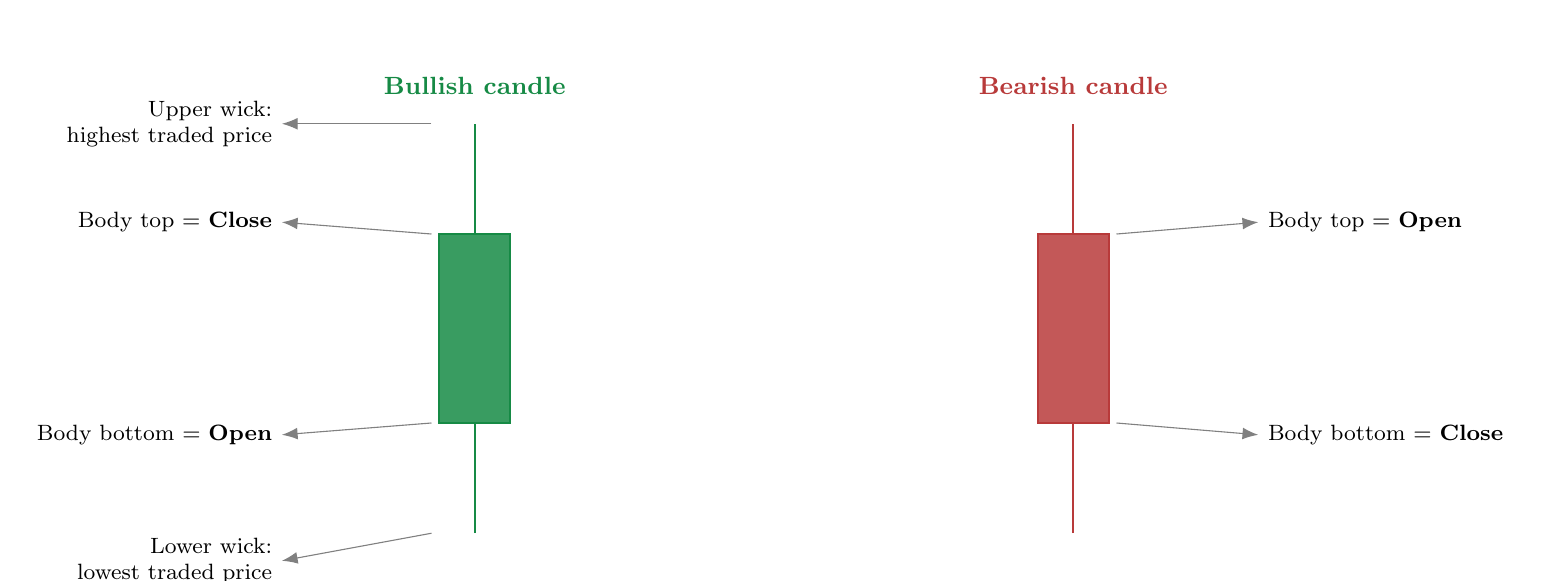
\begin{tikzpicture}[x=1.0cm,y=1.0cm,font=\footnotesize]
  % Green (bullish) candle anatomy
  \draw[bullc,thick] (0,0) -- (0,5.2);
  \fill[bullc!85] (-0.45,1.4) rectangle (0.45,3.8);
  \draw[bullc,thick] (-0.45,1.4) rectangle (0.45,3.8);
  \node[above,align=center,font=\small\bfseries,bullc] at (0,5.45) {Bullish candle};
  \draw[-{Latex[length=2mm]},gray] (-0.55,5.2) -- (-2.45,5.2) node[left,black,align=right]{Upper wick:\\highest traded price};
  \draw[-{Latex[length=2mm]},gray] (-0.55,3.8) -- (-2.45,3.95) node[left,black,align=right]{Body top = \textbf{Close}};
  \draw[-{Latex[length=2mm]},gray] (-0.55,1.4) -- (-2.45,1.25) node[left,black,align=right]{Body bottom = \textbf{Open}};
  \draw[-{Latex[length=2mm]},gray] (-0.55,0) -- (-2.45,-0.35) node[left,black,align=right]{Lower wick:\\lowest traded price};
  % Red (bearish) candle anatomy, shown alongside
  \begin{scope}[xshift=7.6cm]
    \draw[bearc,thick] (0,0) -- (0,5.2);
    \fill[bearc!85] (-0.45,1.4) rectangle (0.45,3.8);
    \draw[bearc,thick] (-0.45,1.4) rectangle (0.45,3.8);
    \node[above,align=center,font=\small\bfseries,bearc] at (0,5.45) {Bearish candle};
    \draw[-{Latex[length=2mm]},gray] (0.55,3.8) -- (2.35,3.95) node[right,black,align=left]{Body top = \textbf{Open}};
    \draw[-{Latex[length=2mm]},gray] (0.55,1.4) -- (2.35,1.25) node[right,black,align=left]{Body bottom = \textbf{Close}};
  \end{scope}
\end{tikzpicture}%
}
\end{center}

\begin{itemize}[leftmargin=*]
    \item \textbf{Open:} The price at the beginning of the period.
    \item \textbf{Close:} The price at the end of the period.
    \item \textbf{High:} The absolute highest price reached during the period.
    \item \textbf{Low:} The absolute lowest price reached during the period.
\end{itemize}

\paragraph{Anatomy of a Candlestick}
\begin{itemize}[leftmargin=*]
    \item \textbf{The Body:} The thick, shaded or colored portion represents the range between the open and close prices.
    \item \textbf{Green/White Body:} Indicates bullish sentiment; the closing price was higher than the opening price. The lower end is the open, and the upper end is the close.
    \item \textbf{Red/Black Body:} Indicates bearish sentiment; the closing price was lower than the opening price. The upper end is the open, and the lower end is the close.
    \item \textbf{The Wicks or Shadows:} The thin lines extending above and below the body show the full trading range, from high to low, during that specific time frame.
\end{itemize}

\subsubsection{Why Use Candlestick Charts?}
Candlestick charts are preferred over simple line charts because they offer a deeper, more immediate understanding of market dynamics.

\begin{itemize}[leftmargin=*]
    \item \textbf{Visual Efficiency:} They provide a quick snapshot of market sentiment, such as bullishness or bearishness, at a glance.
    \item \textbf{Predictive Value:} Specific individual candles or multi-candle patterns can signal potential trend reversals or the continuation of an existing trend.
    \item \textbf{Actionable Insights:} Traders rely on these patterns to identify precise entry and exit points for their trades.
    \item \textbf{Momentum Tracking:} Candlesticks help gauge market momentum and visualize price action better than basic charts. A candlestick chart can convey useful information such as trend, bullishness, bearishness, and volume context.
\end{itemize}

\subsubsection{Analyzing Candlestick Charts for Day Trading}

\paragraph{Time Frames}
Candlesticks represent different durations depending on the selected chart. For instance, in a 5-minute chart, one candle represents 5 minutes of trading; in a 10-minute chart, it represents 10 minutes.

\begin{itemize}[leftmargin=*]
    \item \textbf{Scalping/Day Trading:} 5-minute, 10-minute, or 15-minute charts are used to capture small price fluctuations quickly.
    \item \textbf{Larger Movements:} 30-minute, 1-hour, 3-hour, and daily charts are used to study broader price action.
\end{itemize}

\paragraph{Price Action Analysis}
Reading candlestick charts forms the basis of price action analysis, allowing traders to predict near-future movements by observing current fluctuations. The primary goal in day trading is identifying the overarching trend:

\begin{itemize}[leftmargin=*]
    \item \textbf{Uptrend:} The stock is consistently moving higher. The action bias is to look for long or buy opportunities.
    \item \textbf{Downtrend:} The stock is consistently moving lower. The action bias is to be cautious with long positions or to look for short-side opportunities where appropriate.
\end{itemize}

\paragraph{Assessing Bullish and Bearish Strength}
\begin{itemize}[leftmargin=*]
    \item \textbf{Full Body Candles:} Indicate strong buying when green or strong selling when red because the stock traded strongly through that range.
    \item \textbf{Long Wicks:} A long upper and lower wick on a single candle indicates price volatility: the price swung widely but did not sustain those levels.
    \item \textbf{Wick Positioning:} A body at the upper end with a long lower wick suggests bulls are in control. A body at the lower end with a long upper wick suggests bears are in control.
\end{itemize}

\paragraph{Trend Phases}
\begin{itemize}[leftmargin=*]
    \item \textbf{Trends and Corrections:} A stock rarely moves in a perfectly straight line. A trend often looks like a wave, with periodic moves in the opposite direction before the primary trend resumes. Shortening waves may signal trend exhaustion.
    \item \textbf{Consolidation:} A phase where price moves within a narrow, horizontal range, indicating that neither buyers nor sellers are in firm control. A breakout from consolidation can signal the start of a new trend.
\end{itemize}

\subsection{25 Essential Candlestick Patterns for Trading}
Below is a detailed breakdown of the patterns discussed, categorized by their structural meaning. The diagrams are schematic: green candles close above their open, red candles close below their open, and the surrounding trend or confirmation candle is part of the pattern context.

\subsubsection{Single Candlestick Patterns}

\paragraph{Hammer}
\candlediagram{
    \drawcandle{0}{8.0}{8.9}{3.0}{8.5}{bullc}
}
\begin{itemize}[leftmargin=*]
    \item \textbf{Visual Description:} Small real body near the top of the candle, little or no upper wick, and a long lower wick usually at least twice the body size.
    \item \textbf{How to Identify:} Found near the bottom of a downtrend. It can be red or green, though a green hammer is usually stronger.
    \item \textbf{Interpretation:} Bullish reversal warning. It suggests that the downtrend may be weakening, but confirmation from the next candle is preferred.
    \item \textbf{Psychology:} Sellers pushed the price down sharply, but buyers entered aggressively and forced the close back near the high, rejecting lower prices.
\end{itemize}

\paragraph{Hanging Man}
\candlediagram{
    \drawcandle{0}{8.5}{8.9}{3.0}{8.0}{bearc}
}
\begin{itemize}[leftmargin=*]
    \item \textbf{Visual Description:} Same shape as a hammer: small body near the top, little or no upper wick, and a long lower wick.
    \item \textbf{How to Identify:} Found near the top of an uptrend.
    \item \textbf{Interpretation:} Bearish reversal warning. It is stronger when followed by a red confirmation candle.
    \item \textbf{Psychology:} Sellers managed to push price far below the open during the session. Even if buyers recovered part of the move, the long lower wick warns that selling pressure has appeared after an advance.
\end{itemize}

\paragraph{Inverted Hammer}
\candlediagram{
    \drawcandle{0}{3.5}{9.0}{3.0}{4.0}{bullc}
}
\begin{itemize}[leftmargin=*]
    \item \textbf{Visual Description:} Small body near the bottom of the candle, little or no lower wick, and a long upper wick.
    \item \textbf{How to Identify:} Found near the bottom of a downtrend. It can be red or green.
    \item \textbf{Interpretation:} Bullish reversal warning, especially if the next candle closes higher.
    \item \textbf{Psychology:} Buyers attempted to push price upward, creating the long upper wick. Even though they could not hold the highs, sellers failed to extend the downtrend convincingly.
\end{itemize}

\paragraph{Shooting Star}
\candlediagram{
    \drawcandle{0}{4.0}{9.0}{3.1}{3.5}{bearc}
}
\begin{itemize}[leftmargin=*]
    \item \textbf{Visual Description:} Same shape as an inverted hammer: small body near the bottom and a long upper wick.
    \item \textbf{How to Identify:} Found near the top of an uptrend.
    \item \textbf{Interpretation:} Bearish reversal warning, especially if followed by a red confirmation candle.
    \item \textbf{Psychology:} Buyers pushed price higher, but sellers overwhelmed them and forced the close back near the low, rejecting higher prices.
\end{itemize}

\paragraph{Spinning Top}
\candlediagram{
    \drawcandle{0}{4.8}{8.5}{1.5}{5.2}{bullc}
}
\begin{itemize}[leftmargin=*]
    \item \textbf{Visual Description:} Small real body with long upper and lower wicks of roughly similar length.
    \item \textbf{How to Identify:} Can appear anywhere in a chart.
    \item \textbf{Interpretation:} Indecision or temporary pause. It can precede reversal or continuation depending on the next candles.
    \item \textbf{Psychology:} Both buyers and sellers moved price significantly, but neither side gained dominance, so the close remained near the open.
\end{itemize}

\paragraph{Bullish Spinning Top}
\candlediagram{
    \drawcandle{0}{7.8}{8.2}{5.2}{5.8}{bearc}
    \drawcandle{1}{5.7}{6.1}{3.2}{3.8}{bearc}
    \drawcandle{2}{4.4}{7.0}{1.8}{4.8}{bullc}
    \drawcandle{3}{5.0}{7.4}{4.6}{6.8}{bullc}
}
\begin{itemize}[leftmargin=*]
    \item \textbf{Visual Description:} A spinning top that appears after a downward move and is followed by bullish confirmation.
    \item \textbf{How to Identify:} Found near the bottom of a downtrend, preferably followed by a green candle closing above the spinning top's high.
    \item \textbf{Interpretation:} Potential bullish reversal. The spinning top shows indecision, and the confirmation candle suggests buyers are taking control.
    \item \textbf{Psychology:} Heavy selling pauses and becomes a tug-of-war. The subsequent green candle confirms that buyers have gained the upper hand.
\end{itemize}

\paragraph{Bearish Spinning Top}
\candlediagram{
    \drawcandle{0}{3.2}{5.8}{3.0}{5.4}{bullc}
    \drawcandle{1}{5.2}{7.5}{5.0}{7.1}{bullc}
    \drawcandle{2}{6.4}{9.0}{3.8}{6.0}{bearc}
    \drawcandle{3}{5.8}{6.2}{3.0}{3.6}{bearc}
}
\begin{itemize}[leftmargin=*]
    \item \textbf{Visual Description:} A spinning top that appears after an upward move and is followed by bearish confirmation.
    \item \textbf{How to Identify:} Found near the top of an uptrend, preferably followed by a red candle closing below the spinning top's low.
    \item \textbf{Interpretation:} Potential bearish reversal. The spinning top shows indecision, and the confirmation candle suggests sellers are taking control.
    \item \textbf{Psychology:} Aggressive buying stalls. The subsequent red candle confirms that sellers have taken control from exhausted buyers.
\end{itemize}

\paragraph{Doji}
\candlediagram{
    \drawdoji{0}{5.0}{8.0}{2.0}{black}
}
\begin{itemize}[leftmargin=*]
    \item \textbf{Visual Description:} Almost no real body because open and close prices are virtually identical; it often looks like a plus sign or cross.
    \item \textbf{How to Identify:} Can appear anywhere. Its color is less important than the equality between open and close.
    \item \textbf{Interpretation:} Indecision or possible reversal, especially near the extreme top or bottom of a trend.
    \item \textbf{Psychology:} Represents equilibrium between supply and demand. Neither bulls nor bears could assert dominance during the session.
\end{itemize}

\paragraph{Dragonfly Doji}
\candlediagram{
    \drawdoji{0}{8.0}{8.0}{2.0}{bullc}
}
\begin{itemize}[leftmargin=*]
    \item \textbf{Visual Description:} Looks like a T: open, close, and high are nearly equal, with a long lower wick and little or no upper wick.
    \item \textbf{How to Identify:} Most meaningful near the bottom of a downtrend.
    \item \textbf{Interpretation:} Bullish reversal warning that becomes stronger with a higher close on the next candle.
    \item \textbf{Psychology:} Sellers aggressively pushed price down, but buyers drove price back to the opening high, rejecting lower levels.
\end{itemize}

\paragraph{Gravestone Doji}
\candlediagram{
    \drawdoji{0}{2.0}{8.0}{2.0}{bearc}
}
\begin{itemize}[leftmargin=*]
    \item \textbf{Visual Description:} Looks like an inverted T: open, close, and low are nearly equal, with a long upper wick and little or no lower wick.
    \item \textbf{How to Identify:} Most meaningful near the top of an uptrend.
    \item \textbf{Interpretation:} Bearish reversal warning that becomes stronger with a lower close on the next candle.
    \item \textbf{Psychology:} Buyers pushed price sharply upward, but sellers erased the advance and forced the close back near the low, rejecting higher levels.
\end{itemize}

\paragraph{Marubozu}
\candlediagram{
    \drawcandle{0}{2.0}{8.0}{2.0}{8.0}{bullc}
    \drawcandle{1.2}{8.0}{8.0}{2.0}{2.0}{bearc}
    \node[font=\scriptsize] at (0,-0.3) {Bullish};
    \node[font=\scriptsize] at (1.2,-0.3) {Bearish};
}
\begin{itemize}[leftmargin=*]
    \item \textbf{Visual Description:} A long full-body candle with virtually no upper or lower wick.
    \item \textbf{How to Identify:} Can appear anywhere. A bullish Marubozu opens near the low and closes near the high; a bearish Marubozu opens near the high and closes near the low.
    \item \textbf{Interpretation:} Strong directional conviction. It may signal continuation or reversal depending on trend context and follow-through.
    \item \textbf{Psychology:} Shows one-sided control for nearly the entire session: buyers dominate a green Marubozu, while sellers dominate a red Marubozu.
\end{itemize}

\subsubsection{Multi-Candlestick Patterns}

\paragraph{Bullish Engulfing}
\candlediagram{
    \drawcandle{0}{5.5}{6.0}{4.0}{4.5}{bearc}
    \drawcandle{1}{4.0}{8.0}{3.7}{7.5}{bullc}
}
\begin{itemize}[leftmargin=*]
    \item \textbf{Visual Description:} A small red candle followed by a larger green candle.
    \item \textbf{How to Identify:} Found near the bottom of a downtrend. The second green real body completely engulfs the first red real body.
    \item \textbf{Interpretation:} Bullish reversal signal that is stronger when volume rises or the next candle confirms upward movement.
    \item \textbf{Psychology:} The small red candle shows sellers losing momentum, while the large green candle shows buyers aggressively overwhelming them.
\end{itemize}

\paragraph{Bearish Engulfing}
\candlediagram{
    \drawcandle{0}{4.5}{6.0}{4.0}{5.5}{bullc}
    \drawcandle{1}{7.5}{8.0}{3.7}{4.0}{bearc}
}
\begin{itemize}[leftmargin=*]
    \item \textbf{Visual Description:} A small green candle followed by a larger red candle.
    \item \textbf{How to Identify:} Found near the top of an uptrend. The second red real body completely engulfs the first green real body.
    \item \textbf{Interpretation:} Bearish reversal signal that is stronger when volume rises or the next candle confirms downward movement.
    \item \textbf{Psychology:} The small green candle shows buyers losing momentum, while the large red candle shows sellers aggressively overwhelming them.
\end{itemize}

\paragraph{Bullish Harami}
\candlediagram{
    \drawcandle{0}{8.0}{8.5}{2.5}{3.0}{bearc}
    \drawcandle{1}{4.5}{5.5}{4.2}{5.2}{bullc}
}
\begin{itemize}[leftmargin=*]
    \item \textbf{Visual Description:} A large red candle followed by a smaller green or neutral candle contained inside the previous real body.
    \item \textbf{How to Identify:} Found after a downtrend. The second candle's real body should remain within the first candle's real body.
    \item \textbf{Interpretation:} Potential bullish reversal or loss of bearish momentum, preferably confirmed by a later upward close.
    \item \textbf{Psychology:} Strong selling is followed by a much narrower session, showing that selling pressure has stalled and buyers may be entering.
\end{itemize}

\paragraph{Bearish Harami}
\candlediagram{
    \drawcandle{0}{3.0}{8.5}{2.5}{8.0}{bullc}
    \drawcandle{1}{6.0}{6.3}{5.0}{5.3}{bearc}
}
\begin{itemize}[leftmargin=*]
    \item \textbf{Visual Description:} A large green candle followed by a smaller red or neutral candle contained inside the previous real body.
    \item \textbf{How to Identify:} Found after an uptrend. The second candle's real body should remain within the first candle's real body.
    \item \textbf{Interpretation:} Potential bearish reversal or loss of bullish momentum, preferably confirmed by a later downward close.
    \item \textbf{Psychology:} Strong buying is followed by a much narrower session, showing that buying pressure has stalled and sellers may be entering.
\end{itemize}

\paragraph{Piercing Line}
\candlediagram{
    \drawcandle{0}{8.0}{8.5}{3.0}{3.5}{bearc}
    \drawcandle{1}{2.8}{6.8}{2.5}{6.4}{bullc}
    \draw[dashed,gray] (-0.35,5.75) -- (1.35,5.75);
    \node[font=\scriptsize,gray] at (1.75,5.75) {50\%};
}
\begin{itemize}[leftmargin=*]
    \item \textbf{Visual Description:} A red candle followed by a green candle that opens below the prior candle's low and closes above the midpoint of the prior red body.
    \item \textbf{How to Identify:} Found near the bottom of a downtrend. The green candle should close more than halfway into the previous red body, but usually below the previous open.
    \item \textbf{Interpretation:} Bullish reversal signal that becomes stronger with a subsequent higher close.
    \item \textbf{Psychology:} Sellers initially drive price lower, but buyers forcefully regain control and recover much of the previous session's decline.
\end{itemize}

\paragraph{Dark Cloud Cover}
\candlediagram{
    \drawcandle{0}{3.5}{8.5}{3.0}{8.0}{bullc}
    \drawcandle{1}{8.7}{9.0}{5.0}{5.2}{bearc}
    \draw[dashed,gray] (-0.35,5.75) -- (1.35,5.75);
    \node[font=\scriptsize,gray] at (1.75,5.75) {50\%};
}
\begin{itemize}[leftmargin=*]
    \item \textbf{Visual Description:} A green candle followed by a red candle that opens above the prior high and closes below the midpoint of the prior green body.
    \item \textbf{How to Identify:} Found near the top of an uptrend. The red candle should close deeply into the previous green body.
    \item \textbf{Interpretation:} Bearish reversal signal that becomes stronger with a subsequent lower close.
    \item \textbf{Psychology:} Buyers create an optimistic open, but sellers take control and erase much of the previous session's advance.
\end{itemize}

\paragraph{Morning Star}
\candlediagram{
    \drawcandle{0}{8.0}{8.5}{3.2}{3.5}{bearc}
    \drawcandle{1.2}{2.6}{3.2}{2.2}{2.9}{bullc}
    \drawcandle{2.4}{3.6}{8.5}{3.4}{8.0}{bullc}
}
\begin{itemize}[leftmargin=*]
    \item \textbf{Visual Description:} A three-candle pattern: long red candle, small-bodied candle after a downward gap or weak session, and long green candle.
    \item \textbf{How to Identify:} Found after a downtrend. The third candle should close well into the first candle's body.
    \item \textbf{Interpretation:} Bullish reversal signal indicating that buyers may have taken control.
    \item \textbf{Psychology:} Panic selling slows into indecision, then a strong green candle confirms a shift from bearish to bullish momentum.
\end{itemize}

\paragraph{Evening Star}
\candlediagram{
    \drawcandle{0}{3.5}{8.5}{3.2}{8.0}{bullc}
    \drawcandle{1.2}{8.9}{9.3}{8.4}{8.6}{bearc}
    \drawcandle{2.4}{7.8}{8.0}{3.2}{3.5}{bearc}
}
\begin{itemize}[leftmargin=*]
    \item \textbf{Visual Description:} A three-candle pattern: long green candle, small-bodied candle after an upward gap or strong session, and long red candle.
    \item \textbf{How to Identify:} Found after an uptrend. The third candle should close well into the first candle's body.
    \item \textbf{Interpretation:} Bearish reversal signal indicating that sellers may have taken control.
    \item \textbf{Psychology:} Euphoric buying slows into indecision, then a strong red candle confirms a shift from bullish to bearish momentum.
\end{itemize}

\paragraph{Bullish Abandoned Baby}
\candlediagram{
    \drawcandle{0}{8.0}{8.5}{3.8}{4.0}{bearc}
    \drawdoji{1.2}{2.5}{2.8}{2.2}{black}
    \drawcandle{2.4}{3.8}{8.2}{3.5}{7.8}{bullc}
}
\begin{itemize}[leftmargin=*]
    \item \textbf{Visual Description:} Similar to a Morning Star, but the middle candle is a Doji separated by gaps on both sides.
    \item \textbf{How to Identify:} Found after a downtrend. The Doji should be isolated below the first and third candles.
    \item \textbf{Interpretation:} Strong bullish reversal signal, especially when the third candle closes firmly upward.
    \item \textbf{Psychology:} Sellers exhaust themselves into an isolated Doji, then buyers take control with a sharp move upward.
\end{itemize}

\paragraph{Bearish Abandoned Baby}
\candlediagram{
    \drawcandle{0}{4.0}{8.2}{3.8}{8.0}{bullc}
    \drawdoji{1.2}{9.0}{9.3}{8.7}{black}
    \drawcandle{2.4}{8.2}{8.5}{3.8}{4.0}{bearc}
}
\begin{itemize}[leftmargin=*]
    \item \textbf{Visual Description:} Similar to an Evening Star, but the middle candle is a Doji separated by gaps on both sides.
    \item \textbf{How to Identify:} Found after an uptrend. The Doji should be isolated above the first and third candles.
    \item \textbf{Interpretation:} Strong bearish reversal signal, especially when the third candle closes firmly downward.
    \item \textbf{Psychology:} Buyers exhaust themselves into an isolated Doji, then sellers take control with a sharp move downward.
\end{itemize}

\paragraph{Three White Soldiers}
\candlediagram{
    \drawcandle{0}{2.5}{5.8}{2.2}{5.5}{bullc}
    \drawcandle{1}{4.8}{7.5}{4.5}{7.2}{bullc}
    \drawcandle{2}{6.5}{9.0}{6.2}{8.8}{bullc}
}
\begin{itemize}[leftmargin=*]
    \item \textbf{Visual Description:} Three consecutive long green candles, each closing higher than the previous candle.
    \item \textbf{How to Identify:} Found after a downtrend. Each candle typically opens within the previous candle's real body and closes near its high.
    \item \textbf{Interpretation:} Strong bullish reversal or continuation signal, but traders should avoid chasing if the candles are extremely extended.
    \item \textbf{Psychology:} Sustained buying pressure over three periods overwhelms remaining sellers from the prior downtrend.
\end{itemize}

\paragraph{Three Black Crows}
\candlediagram{
    \drawcandle{0}{8.8}{9.0}{5.8}{6.0}{bearc}
    \drawcandle{1}{6.8}{7.0}{4.0}{4.2}{bearc}
    \drawcandle{2}{5.0}{5.2}{2.2}{2.5}{bearc}
}
\begin{itemize}[leftmargin=*]
    \item \textbf{Visual Description:} Three consecutive long red candles, each closing lower than the previous candle.
    \item \textbf{How to Identify:} Found after an uptrend. Each candle typically opens within the previous candle's real body and closes near its low.
    \item \textbf{Interpretation:} Strong bearish reversal or continuation signal, but traders should avoid chasing if the candles are extremely extended.
    \item \textbf{Psychology:} Sustained selling pressure over three periods overwhelms remaining buyers from the prior uptrend.
\end{itemize}

\paragraph{Gap Up}
\candlediagram{
    \drawcandle{0}{3.0}{5.0}{2.0}{4.2}{bullc}
    \drawcandle{1.2}{6.2}{8.5}{6.0}{8.0}{bullc}
    \draw[<->,gray] (0.6,5.05) -- (0.6,5.95);
    \node[font=\scriptsize,gray] at (1.15,5.5) {gap};
}
\begin{itemize}[leftmargin=*]
    \item \textbf{Visual Description:} A new candle opens and trades above the previous candle's high, leaving visible empty space on the chart.
    \item \textbf{How to Identify:} The second candle's low is above the first candle's high.
    \item \textbf{Interpretation:} Strong bullish sentiment or positive repricing; follow-through depends on volume and whether the gap holds.
    \item \textbf{Psychology:} Buyers are eager enough to pay significantly higher prices immediately, bypassing lower levels.
\end{itemize}

\paragraph{Gap Down}
\candlediagram{
    \drawcandle{0}{7.2}{8.5}{6.0}{6.3}{bearc}
    \drawcandle{1.2}{4.0}{5.0}{2.0}{3.0}{bearc}
    \draw[<->,gray] (0.6,5.05) -- (0.6,5.95);
    \node[font=\scriptsize,gray] at (1.15,5.5) {gap};
}
\begin{itemize}[leftmargin=*]
    \item \textbf{Visual Description:} A new candle opens and trades below the previous candle's low, leaving visible empty space on the chart.
    \item \textbf{How to Identify:} The second candle's high is below the first candle's low.
    \item \textbf{Interpretation:} Strong bearish sentiment or sudden negative repricing. Follow-through depends on volume and whether the gap holds.
    \item \textbf{Psychology:} Sellers are urgent enough to accept significantly lower prices immediately, bypassing higher levels.
\end{itemize}

\subsubsection{Expert Trading Advice}
While patterns are powerful, they should not be traded blindly.

\begin{itemize}[leftmargin=*]
    \item \textbf{Wait for Confirmation:} Do not take action based on a single pattern formation. Wait for subsequent candles to confirm the anticipated direction.
    \item \textbf{Consider Macro Context:} Market conditions and breaking news, such as border tensions, regulatory changes, or dividend announcements, can cause sudden shifts that override technical chart patterns.
    \item \textbf{Use Confluence:} Successful traders combine candlestick patterns with other technical indicators and comprehensive trading strategies to increase their probability of success.
\end{itemize}


\subsection{Volume in the Stock Market}
\index{Volume}
\index{Relative Volume}
\index{On-Balance Volume}
\index{Chaikin Money Flow}
\index{Klinger Oscillator}

\subsubsection{What is Trading Volume?}
In stock trading, \textbf{volume} represents the total number of financial assets, such as shares or contracts, that change hands during a specific timeframe. It is a critical indicator of market activity, liquidity, and sentiment.

\begin{itemize}[leftmargin=*]
    \item \textbf{Stocks:} Measured by the number of shares traded.
    \item \textbf{Futures \& Options:} Measured by the number of contracts traded.
\end{itemize}

\paragraph{Why Volume Matters}
\begin{itemize}[leftmargin=*]
    \item \textbf{High Volume:} Indicates high liquidity and strong market interest. It allows traders to enter and exit large positions more easily without significantly affecting the asset's price.
    \item \textbf{Low Volume:} Suggests limited interest and low liquidity, making it difficult to execute large trades without causing erratic price shifts.
    \item \textbf{Timing:} Volume typically peaks during the opening and closing periods of a trading session.
\end{itemize}

\subsubsection{Relative Volume (RVOL)}
While raw volume provides the total number of trades, \textbf{Relative Volume (RVOL)} determines whether that level of activity is normal or unusually high for a specific asset.

RVOL is a ratio that compares current activity to historical averages:

\begin{equation*}
    RVOL = \frac{\text{Current Volume}}{\text{Average Historical Volume}}
\end{equation*}

\begin{quote}
\textit{Example: If a stock's historical average is 500,000 shares per day, but it has traded 1,000,000 shares today, the RVOL is 2, meaning it is trading at twice its normal activity.}
\end{quote}

\paragraph{The Importance of RVOL}
\begin{itemize}[leftmargin=*]
    \item \textbf{Highlights Unusual Activity:} High RVOL is often a direct reaction to earnings reports, breaking news, or macroeconomic triggers.
    \item \textbf{Confirms Price Moves:} Breakouts or price trends accompanied by high RVOL are significantly more reliable and more likely to sustain.
    \item \textbf{Indicates Liquidity:} A high RVOL generally implies better liquidity during that specific trading session.
\end{itemize}

\subsubsection{The Relationship Between Price and Volume}
Traders continuously analyze volume alongside price action to gauge the true strength of a market move. Volume acts as an important confirmation tool.

\begin{itemize}[leftmargin=*]
    \item \textbf{Rising price with increasing volume:} Bullish momentum; the upward trend is backed by genuine buying conviction.
    \item \textbf{Falling price with decreasing volume:} Downward trend with waning participation.
    \item \textbf{Price and volume moving in opposite directions:} Uncertainty or potential reversal; the current trend lacks conviction, so a major change in trend direction becomes more probable.
\end{itemize}

\begin{quote}
\textit{Note: High volume does not inherently mean a stock's price will rise; heavy volume on a red candle signifies immense selling pressure.}
\end{quote}

\subsubsection{Key Volume Indicators}
Volume indicators apply mathematical formulas to raw volume data, producing visual overlays that help traders confirm trends, spot divergences, and identify entry/exit points.

\paragraph{On-Balance Volume (OBV)}
Created by Joseph Granville in 1963, OBV is a cumulative indicator that measures buying and selling pressure to reflect crowd sentiment.

\begin{itemize}[leftmargin=*]
    \item If the current closing price is \textbf{greater} than the previous close:
    \begin{equation*}
        OBV_{\text{current}} = OBV_{\text{previous}} + \text{Volume}_{\text{current}}
    \end{equation*}

    \item If the current closing price is \textbf{less} than the previous close:
    \begin{equation*}
        OBV_{\text{current}} = OBV_{\text{previous}} - \text{Volume}_{\text{current}}
    \end{equation*}

    \item If the current closing price is \textbf{equal} to the previous close:
    \begin{equation*}
        OBV_{\text{current}} = OBV_{\text{previous}}
    \end{equation*}
\end{itemize}

\paragraph{Chaikin Money Flow (CMF)}
Developed by Marc Chaikin in the 1980s, CMF identifies short-term money-flow divergence. It uses a standard 21-day period to measure the volume-weighted average of buying and selling. Values oscillate between $+1$, indicating strong buying, and $-1$, indicating strong selling, with the zero line representing equilibrium.

\begin{enumerate}[leftmargin=*]
    \item \textbf{Step 1: Calculate the Money Flow Multiplier.}
    \begin{equation*}
        \text{Multiplier} = \frac{(\text{Close} - \text{Low}) - (\text{High} - \text{Low})}{\text{High} - \text{Low}}
    \end{equation*}

    \item \textbf{Step 2: Calculate the Money Flow Volume.}
    \begin{equation*}
        \text{MFV} = \text{Multiplier} \times \text{Volume}
    \end{equation*}

    \item \textbf{Step 3: Calculate the CMF.}
    \begin{equation*}
        CMF = \frac{\text{21-day Average of Daily MFV}}{\text{21-day Average of Volume}}
    \end{equation*}
\end{enumerate}

\paragraph{Klinger Oscillator}
Developed by Stephen Klinger in 1977, this tool measures the long-term trend of money flow while remaining highly sensitive to short-term price fluctuations. It relies heavily on Volume Force and Exponential Moving Averages (EMA).

\subsubsection{Interpreting Volume Data on Charts}
Trading volume is typically displayed at the bottom of an asset's candlestick price chart as a series of vertical bars.

\begin{itemize}[leftmargin=*]
    \item \textbf{Green Volume Bars (Buying Volume):} Indicates transactions primarily settled at the ask price, pushing the stock price upward.
    \item \textbf{Red Volume Bars (Selling Volume):} Indicates transactions primarily settled at the bid price, exerting downward pressure on the stock price.
\end{itemize}

Volume data can be adjusted to any time frame, such as hourly, daily, or weekly, and is widely accessible through broker platforms, stock exchanges, and financial news sites. Used correctly, it allows investors to distinguish between a minor price pull-back and a structural market reversal.


\section{How Do Stock Prices Change?}
\index{Stock prices}
\index{Supply and demand}
\index{Order book}
\index{Market microstructure}

\subsection{Dynamics of Stock Prices and Market Microstructure}

\subsubsection{Why Do Stock Prices Change?}
Stock prices are inherently unpredictable and fluctuate based on a complex interaction of microeconomic and macroeconomic variables. These variables fundamentally alter the supply and demand for a specific asset.

\paragraph{Supply and Demand}
\begin{itemize}[leftmargin=*]
    \item \textbf{The Core Principle:} Supply and demand form the foundational driver of all markets. If demand for a stock is high while supply is limited, the price increases. Conversely, if there is a surplus of sellers, meaning high supply, and few buyers, meaning low demand, the price decreases.
\end{itemize}

\paragraph{Company Performance: Fundamentals}
\begin{itemize}[leftmargin=*]
    \item \textbf{Positive Drivers:} Strong earnings reports, new product launches, strategic acquisitions, and business expansions can boost investor confidence and drive valuations higher.
    \item \textbf{Negative Drivers:} Poor earnings, legal lawsuits, management controversies, and operational setbacks can erode confidence and cause prices to drop.
\end{itemize}

\paragraph{Economic Factors: Macroeconomics}
\begin{itemize}[leftmargin=*]
    \item \textbf{Key Indicators:} Broader economic conditions such as interest rates, inflation, GDP growth, and employment levels influence the entire market.
    \item \textbf{Example:} Lower interest rates combined with robust economic growth typically support higher stock prices, because borrowing is cheap and investors are optimistic about future corporate expansion.
\end{itemize}

\paragraph{Industry Trends and Competition}
\begin{itemize}[leftmargin=*]
    \item \textbf{Sector Tailwinds:} Technological advancements, surging consumer demand, and favorable regulatory shifts can elevate expectations for entire industries.
    \item \textbf{Sector Headwinds:} Increased competition, structural industry disruptions, and declining demand can negatively affect investor expectations and suppress prices.
\end{itemize}

\paragraph{Investor Sentiment and Market Psychology}
\begin{itemize}[leftmargin=*]
    \item \textbf{Emotional Drivers:} Market movements are heavily influenced by human psychology, especially confidence, fear, uncertainty, speculation, and momentum trading.
    \item \textbf{Impact:} These behavioral factors frequently drive sharp short-term price fluctuations that may temporarily diverge from a company's underlying fundamentals.
\end{itemize}

\paragraph{Political and Geopolitical Events}
\begin{itemize}[leftmargin=*]
    \item \textbf{Catalysts for Volatility:} Elections, changes in government policies, tax reforms, trade agreements, and international conflicts inject uncertainty into the market and can abruptly alter investor behavior and asset pricing.
\end{itemize}

\subsection{Understanding Price Determination: The Order Book}
To understand exactly how the factors above translate into a specific market price, one must understand the exchange's matching mechanism.

\subsubsection{What is an Order Book?}
An order book, also known as a \textbf{continuous book}, is a real-time electronic ledger maintained by a financial exchange. It records and displays all outstanding buy and sell orders for a specific financial asset, such as stocks, derivatives, bonds, or currencies.

\begin{itemize}[leftmargin=*]
    \item \textbf{Structure:} It organizes \textbf{bid} orders, or buy offers, and \textbf{ask} orders, or sell offers, by price level.
    \item \textbf{Contents:} It houses various order types, including market orders, limit orders, stop-loss orders, and trailing stop-loss orders.
\end{itemize}

\subsubsection{Key Insights Provided by the Order Book}
Because the order book updates continuously throughout the trading day, observing how orders accumulate, execute, or get canceled allows traders to gauge:

\begin{itemize}[leftmargin=*]
    \item Real-time market sentiment and short-term buying or selling pressure.
    \item Market depth and order imbalances.
    \item The spread between the highest bid and the lowest ask.
    \item Participant activity, which can help distinguish between retail activity and large institutional flows.
\end{itemize}

\subsubsection{Advantages \& Trading Strategies}
\begin{enumerate}[leftmargin=*]
    \item \textbf{Identifying Support and Resistance:} By locating price levels with large concentrations of buy orders, or support, and sell orders, or resistance, traders can anticipate where a stock's price is likely to bounce or stall.
    \item \textbf{Trend Analysis \& Reversals:} Traders monitor the book to determine whether a current trend has the momentum to continue or whether order flow suggests that the market is about to reverse, helping guide precise entry and exit points.
    \item \textbf{Algorithmic \& Quantitative Trading:} Market participants who favor technical analysis over fundamental analysis rely heavily on order book data to build automated trading algorithms and seek a quantitative edge.
    \item \textbf{Transparency \& Regulation:} While some institutional entities attempt to conceal trades using dark pools, the general transparency of the order book allows regulatory bodies, such as the SEC, to monitor for market delinquencies, fraud, and manipulation.
\end{enumerate}

\subsubsection{Real-World Example: NASDAQ TotalView}
\begin{itemize}[leftmargin=*]
    \item NASDAQ TotalView is regarded as one of the most comprehensive order books in the US and globally. It provides deep data for securities listed on both the NASDAQ and NYSE, equipping traders, investors, and analysts with historical trading volumes, precise price data, and advanced tools for navigating the markets.
\end{itemize}

\subsection{Bid-Ask Spread: Study Notes}
\index{Bid-ask spread}
\index{Market microstructure!bid-ask spread}
\index{Liquidity!bid-ask spread}
\index{Market makers}
\index{Transaction costs}
\index{Effective spread}

\subsubsection{What Is the Bid-Ask Spread?}
Every tradable security has \textbf{two simultaneously quoted prices} at any moment, not one:

\begin{itemize}[leftmargin=*]
    \item \textbf{Bid Price:} The highest price a buyer, trader, investor, or market maker is currently willing to \textbf{pay} to purchase the security.
    \item \textbf{Ask Price or Offer Price:} The lowest price a seller or market maker is currently willing to \textbf{accept} to sell the security.
\end{itemize}

The \textbf{bid-ask spread} is the difference between these two prices:

\begin{equation*}
    \boxed{\text{Bid-Ask Spread} = \text{Ask Price} - \text{Bid Price}}
\end{equation*}

The spread is much more than a technical detail. It is simultaneously the principal transaction cost of trading outside explicit commissions, a real-time barometer of market liquidity, and a reflection of supply-demand dynamics, market-maker risk, and overall market structure.

\subsubsection{The Two Key Players in Every Transaction}
Understanding the spread requires identifying who stands on each side of a trade.

\begin{description}[leftmargin=*,style=nextline]
    \item[Price Taker: Trader or Investor] The party that \textbf{initiates} a trade by accepting a currently quoted price. Price takers demand immediacy: they want to buy or sell right now. To \textbf{buy}, they pay the \textbf{ask price}; to \textbf{sell}, they receive the \textbf{bid price}.
    \item[Market Maker: Counterparty] The party that \textbf{stands ready} to buy or sell at any time by continuously quoting two-sided prices, meaning both bid and ask quotes. Market makers can be brokerage-employed traders, independent proprietary trading firms, or electronic systems and algorithms.
\end{description}

Market makers provide immediacy to price takers and earn compensation through the spread. A market maker \textbf{buys} at the \textbf{bid price} from sellers and \textbf{sells} at the \textbf{ask price} to buyers.

\begin{quote}
\textit{Key insight: The spread is the market maker's compensation for providing immediacy and for assuming inventory risk.}
\end{quote}

\subsubsection{The Spread as Transaction Cost}
When a trader executes a market order, they buy at the ask and sell at the bid. Therefore, the round-trip cost of entering and exiting a position is effectively the spread. The trader starts underwater by exactly the spread amount the moment the position is entered. This is what brokerages mean when they say revenue comes from traders \textbf{crossing the spread}.

This matters even in commission-free trading. A trade may have no explicit commission, but it is not truly free if the execution cost is embedded in the bid-ask spread.

\subsubsection{Order Book Depth and How It Shapes the Spread}
The spread is not fixed. It is a dynamic result of \textbf{resting limit orders} in the order book.

\begin{itemize}[leftmargin=*]
    \item \textbf{Many bid limit orders:} Competitive buyers push the highest bid upward, creating a \textbf{narrower spread}.
    \item \textbf{Few bid limit orders:} Weak demand causes the highest bid to fall, creating a \textbf{wider spread}.
    \item \textbf{Many ask limit orders:} Competitive sellers push the lowest ask downward, creating a \textbf{narrower spread}.
    \item \textbf{Few ask limit orders:} Limited selling interest causes the lowest ask to rise, creating a \textbf{wider spread}.
\end{itemize}

\paragraph{Practical implication:} When placing a buy-limit order, always check the current spread. If the limit price sits inside the spread but no counterparty is willing to meet it, the order will remain unfilled.

\subsubsection{Spread Calculations: From Basic to Advanced}
The most basic formula is:

\begin{equation*}
    \text{Spread} = \text{Ask} - \text{Bid}
\end{equation*}

For example, if the bid is \$19 and the ask is \$20, then the spread is \$1.00.

\paragraph{Percentage Spread}
The percentage spread converts the dollar spread into a relative metric that is useful for comparing securities with different price levels:

\begin{equation*}
    \text{Percentage Spread} = \frac{\text{Ask} - \text{Bid}}{\text{Ask}} \times 100\%
\end{equation*}

For example, if the spread is \$1 and the ask is \$20, then the percentage spread is $5\%$. This makes the cost meaningful in context: a \$1 spread on a \$20 stock is far more significant than the same \$1 spread on a \$500 stock, where it is only $0.2\%$.

\begin{quote}
\textit{Note: Some formulations use the midpoint or the current stock price as the denominator instead of the ask. The key is to use a consistent base for comparison.}
\end{quote}

\paragraph{Midpoint}
The midpoint is the theoretical fair price between buyers and sellers:

\begin{equation*}
    \text{Midpoint} = \frac{\text{Bid} + \text{Ask}}{2}
\end{equation*}

It is a key reference point for calculating the effective spread and assessing price improvement.

\paragraph{Effective Spread}
The \textbf{effective spread} measures the actual cost of a completed market order. It accounts for the possibility that an order may receive \textbf{price improvement}, meaning it fills better than the quoted price, or may \textbf{walk the book}, meaning it fills worse than the top quote because the order consumes multiple price levels.

For a buy order:

\begin{align*}
    \text{Effective Half-Spread} &= \text{Execution Price} - \text{Midpoint}, \\
    \text{Effective Spread} &= 2 \times (\text{Execution Price} - \text{Midpoint}).
\end{align*}

For a sell order:

\begin{equation*}
    \text{Effective Spread} = 2 \times (\text{Midpoint} - \text{Execution Price}).
\end{equation*}

For example, if the midpoint is \$20.00 and a market buy fills at \$20.05, then the effective half-spread is \$0.05 and the effective round-trip spread is \$0.10. The effective spread is a more accurate measure of true trading cost than the quoted spread, especially in highly liquid markets where quote-to-fill differences are common.

\paragraph{Weighted Average Spread}
In a layered order book with multiple price levels, the quoted best bid and best ask only show the top of the book. Larger orders can consume multiple levels, making the true execution cost higher. A \textbf{weighted average spread} accounts for this by:

\begin{enumerate}[leftmargin=*]
    \item Weighting each price tier by the volume available at that level.
    \item Computing a volume-weighted average ask and a volume-weighted average bid.
    \item Defining the weighted spread as the weighted average ask minus the weighted average bid.
\end{enumerate}

This is especially important for institutional traders executing large block orders, because the simple quoted spread may dramatically understate execution cost.

\subsubsection{The Spread as a Liquidity Measure}
\textbf{Market liquidity} is the ease with which an asset can be bought or sold without materially moving its price. The bid-ask spread is one of the most direct real-time measures of liquidity:

\begin{align*}
    \text{Narrow spread} &\Rightarrow \text{High liquidity}, \\
    \text{Wide spread} &\Rightarrow \text{Low liquidity}.
\end{align*}

\paragraph{Supply and Demand of Liquidity}
Price takers \textbf{demand liquidity} because they want immediate execution. Market makers \textbf{supply liquidity} by posting prices at which immediate trades can occur. The spread is therefore the \textbf{price of immediacy}.

Typical spread behavior varies across markets:

\begin{itemize}[leftmargin=*]
    \item \textbf{Major FX pairs, such as EUR/USD:} Very narrow spreads, often around $0.01\%$ or fractions of a penny.
    \item \textbf{Large-cap US stocks, such as AAPL or MSFT:} Spreads are often just pennies, commonly around \$0.01.
    \item \textbf{Small-cap stocks:} Spreads can reach $1$--$2\%$ of the ask price or more.
    \item \textbf{Exotic derivatives and options:} Spreads can be very wide relative to the instrument's price.
\end{itemize}

\paragraph{Perceived Risk and Inventory Risk}
Spreads also reflect \textbf{market-maker risk}. Wider spreads are demanded when:

\begin{itemize}[leftmargin=*]
    \item The security's price can move rapidly and unpredictably, meaning volatility is high.
    \item The market maker faces \textbf{adverse selection}, or the risk of trading against a counterparty with superior information.
    \item Hedging costs are high, as with complex derivatives.
\end{itemize}

Options and futures often show spreads that are a much larger percentage of their price than equities or FX because of these risk and hedging considerations.

\subsubsection{Factors That Determine Spread Width}
Seven key factors shape the spread at any moment, and they are deeply interrelated:

\begin{enumerate}[leftmargin=*]
    \item \textbf{Market Liquidity:} More buyers and sellers create more competition and a tighter spread. Fewer participants create wider spreads.
    \item \textbf{Volatility:} Higher price uncertainty causes market makers to widen spreads to protect against adverse price moves between quote and execution. Earnings announcements, geopolitical events, and major macroeconomic releases often cause temporary spread widening.
    \item \textbf{Trading Volume:} Higher volume typically narrows spreads through increased efficiency. However, a volume spike in an inherently illiquid stock may not narrow the spread if the underlying order-book depth remains thin.
    \item \textbf{Asset Class:} Large-cap equities usually have narrow spreads; small-cap equities are wider; major FX pairs are among the tightest globally; exotic currencies and OTC derivatives can be wide; options and futures can be wide relative to price.
    \item \textbf{Time of Day:} Market open and close often have high activity and relatively tight spreads, while midday lulls can widen spreads. In FX, the London/New York overlap is often the most liquid window. Major announcements, such as central-bank decisions, can widen spreads sharply around the release before normalization.
    \item \textbf{Market Structure and Competition:} Electronic limit order books with many participants create intense competition and tight spreads. OTC markets with fewer participants, lower transparency, and higher search costs tend to have wider spreads.
    \item \textbf{Market-Maker Risk Perception:} If a market maker perceives elevated risk in a specific security, such as a rumored takeover, upcoming FDA ruling, or earnings uncertainty, they may widen the spread as self-protection.
\end{enumerate}

\subsubsection{The Role of Market Makers}
Market makers are the structural backbone of the bid-ask spread. Their key functions are:

\begin{enumerate}[leftmargin=*]
    \item \textbf{Providing Liquidity:} They continuously quote two-sided prices so buyers and sellers can find a counterparty without waiting for a natural match.
    \item \textbf{Narrowing Spreads Through Competition:} Multiple market makers compete for order flow by offering the highest bid and lowest ask, compressing spreads for all participants.
    \item \textbf{Managing Risk and Inventory:} Each trade leaves the market maker with a long or short inventory position. The spread compensates them for this risk. If they are overly long, they may lower both bid and ask to discourage additional buys and attract sellers. If they are overly short, they may raise both bid and ask to discourage sells and attract buyers.
    \item \textbf{Adapting to Market Conditions:} During high volatility or low liquidity, market makers widen spreads to account for higher adverse price risk. They continuously recalibrate quotes based on order flow, news, and price action.
    \item \textbf{Enhancing Market Efficiency:} By posting competitive prices, market makers help align executed prices with fair value and make prices more informative.
    \item \textbf{Supporting Orderly Order Flow:} Market makers absorb imbalances between buy and sell orders, preventing sudden price spikes from one-sided order pressure and smoothing price discovery.
\end{enumerate}

\subsubsection{Market Orders vs. Limit Orders: Practical Implications}
Order choice determines whether a trader pays or avoids the spread:

\begin{itemize}[leftmargin=*]
    \item \textbf{Market Order:} A buy market order pays the ask, and a sell market order receives the bid. The trader acts as a \textbf{liquidity taker} and effectively pays the full spread.
    \item \textbf{Limit Order:} The trader specifies the execution price. If the order fills at that price, the trader acts as a \textbf{liquidity provider} and may avoid paying the spread, though execution is not guaranteed.
\end{itemize}

\begin{quote}
\textit{Practical rule: When the spread is wide or shifting rapidly, avoid market orders when possible. Use limit orders to specify the exact price and reduce the risk of an unfavorable fill.}
\end{quote}

The round-trip cost with a market order equals buying at the ask and selling at the bid, so the implicit cost equals the full spread per unit.

\subsubsection{Bid-Ask Spread and Arbitrage}
\paragraph{Cross-Market Arbitrage}
Arbitrageurs exploit price discrepancies across venues. For example, if Exchange A quotes stock XYZ with a bid of \$100 while Exchange B quotes the same stock with an ask of \$99, an arbitrageur can simultaneously buy at \$99 on Exchange B and sell at \$100 on Exchange A, earning \$1 per share before costs. Such opportunities usually disappear in milliseconds once discovered.

\paragraph{Market-Making as Arbitrage}
Some algorithmic traders act as informal market makers by posting both bid and ask quotes to capture the spread itself. This is effectively arbitrage between the bid and the ask within a single market, though traders must manage net inventory risk through dynamic quote adjustment.

\paragraph{Technology Dependency}
Spread-based arbitrage is highly technology-driven. Important requirements include co-location, meaning servers placed physically near exchange matching engines; ultra-low-latency data feeds; and execution algorithms that can react in microseconds. Once an opportunity is discovered and acted upon, it disappears as other participants respond.

\subsubsection{Worked Examples}
\paragraph{Example 1: Basic Spread}
For stock XYZ, suppose the bid is \$19.00 and the ask is \$20.00. The spread is \$1.00, and the percentage spread is:

\begin{equation*}
    \frac{\$1}{\$20} \times 100\% = 5\%.
\end{equation*}

The spread narrows if a buyer raises the bid to \$19.50 or a seller lowers the ask to \$19.80.

\paragraph{Example 2: Large Trade Cost}
Suppose Apple stock has a bid of \$50.00 and an ask of \$50.05. The spread is only \$0.05, which appears trivial. However, if a trader buys 100 shares at market, they pay \$50.05 per share. The immediate theoretical sale value is \$50.00 per share, so the implicit spread cost is:

\begin{equation*}
    100 \times \$0.05 = \$5.00.
\end{equation*}

At institutional scale, a 10,000-share trade creates an implicit cost of \$500 from the spread alone. This illustrates why even tiny spreads matter at scale and why large traders focus heavily on execution quality.


\section{Stock Market Index}
\index{Stock market index}
\index{Nifty 50}
\index{Sensex}
\index{Market capitalization weighting}
\index{Free-float market capitalization}
\index{Index divisor}

\subsection{Stock Market Indices}

\subsubsection{What is a Stock Market Index?}
Tracking the individual performance of every listed company to determine the overall market direction is practically difficult because major exchanges contain thousands of listed securities. A \textbf{stock market index} solves this problem by grouping a specific selection of companies into a representative basket.

By observing a single index value, investors can quickly gauge the broad direction, sentiment, and risk appetite of a market segment. An index therefore acts like a market thermometer: it does not show every individual company's movement, but it gives a reliable summary of the selected market universe.

\subsubsection{Major Indian Broad-Market Indices}
The two primary indices that serve as bellwethers for the Indian stock market are:

\begin{itemize}[leftmargin=*]
    \item \textbf{Nifty 50:} Managed by the National Stock Exchange ecosystem through NSE Indices. It comprises 50 large-cap companies and is often remembered using the phrase \emph{Nifty Fifty}.
    \item \textbf{BSE Sensex:} Managed by BSE Limited. ``Sensex'' is short for \emph{Sensitivity Index}. It comprises 30 large-cap companies.
\end{itemize}

\paragraph{Correlation Between Nifty and Sensex}
Nifty and Sensex generally move in similar directions because both are broad-market large-cap indices and many of their constituent companies overlap. It is therefore uncommon for one to be sharply positive while the other is sharply negative, unless the difference is driven by index-specific weights or constituent-specific news.

\subsubsection{Categories of Indices}
Indices are categorized based on the segment of the market they are designed to track.

\begin{enumerate}[leftmargin=*]
    \item \textbf{Market-Capitalization Indices:} These track companies based on size.
    \begin{itemize}[leftmargin=*]
        \item \textbf{Large-Cap:} Nifty 50 and Sensex.
        \item \textbf{Mid-Cap:} Nifty Midcap indices.
        \item \textbf{Small-Cap:} Nifty Smallcap indices.
    \end{itemize}

    \item \textbf{Sector-Specific Indices:} These track companies within a particular industry or economic sector.
    \begin{itemize}[leftmargin=*]
        \item \textbf{Bank Nifty:} Comprises major banking stocks.
        \item \textbf{Fin Nifty:} Comprises financial services companies, including banks and other financial institutions.
    \end{itemize}

    \item \textbf{Strategy or Factor Indices:} These track companies based on rules such as low volatility, quality, momentum, dividend yield, or value characteristics.

    \item \textbf{Thematic Indices:} These track a market theme, such as consumption, infrastructure, technology, or energy transition.
\end{enumerate}

\subsubsection{The Core Uses of an Index}
Indices serve several important functions for market participants.

\paragraph{Benchmarking: Performance Evaluation}
An index provides a standard benchmark against which an investor can measure portfolio performance.

\begin{itemize}[leftmargin=*]
    \item \textbf{Example:} If a portfolio generates a 20\% return in a year, that may appear successful. However, if the Nifty 50 generated a 30\% return over the same period, the portfolio underperformed the broader large-cap market.
    \item \textbf{Application:} The benchmark should match the portfolio universe. A large-cap portfolio should be compared with Nifty 50 or Sensex, while a small-cap portfolio should be compared with a relevant small-cap index.
\end{itemize}

\paragraph{Trading and Derivatives}
The base index itself, often called the \textbf{spot index}, is only a calculated number and cannot be directly bought or sold like a stock. However, traders actively trade index-linked instruments in the derivatives market.

\begin{itemize}[leftmargin=*]
    \item Traders buy and sell \textbf{Futures and Options (F\&O)} contracts based on indices such as Nifty, Bank Nifty, and Fin Nifty.
    \item Unlike the spot index, derivative contracts have active buyers, sellers, bids, asks, expiries, and tradable prices on broker terminals.
\end{itemize}

\paragraph{Market Sentiment and Economic Signalling}
Indices summarize whether a market segment is broadly risk-on or risk-off. A rising broad-market index usually indicates positive sentiment, while a falling index indicates caution, pessimism, or selling pressure.

\paragraph{Passive Investing}
Index funds and exchange traded funds (ETFs) replicate indices so investors can gain diversified exposure without selecting individual stocks. This is one reason index construction methodology matters: it determines what passive investors ultimately own.

\subsection{Index Construction Methodology}
Indices are not usually simple averages where every company has equal importance. Most major equity indices use a \textbf{market-capitalization weighted methodology}, often specifically a \textbf{free-float market-capitalization weighted methodology}. This means larger companies receive higher weights and therefore have greater influence on index movement.

\subsubsection{Market Capitalization: The Starting Point}
A company's market capitalization is its total equity value in the stock market:

\begin{equation*}
    \text{Market Capitalization} = \text{Share Price} \times \text{Total Shares Outstanding}.
\end{equation*}

For example, if a company has 100 crore shares outstanding and each share trades at Rs. 200, its market capitalization is:

\begin{equation*}
    100 \text{ crore} \times 200 = \text{Rs. }20{,}000 \text{ crore}.
\end{equation*}

A market-cap weighted index gives more weight to companies with larger market capitalizations because these companies represent a larger share of the total investable equity market.

\subsubsection{Free-Float Market Capitalization}
Many modern indices use \textbf{free-float market capitalization} rather than total market capitalization. Free float refers to the shares that are actually available for public trading. Shares held by promoters, governments, strategic investors, or locked-in shareholders are often excluded because they do not freely trade in the market.

\begin{equation*}
    \text{Free-Float Market Cap} = \text{Share Price} \times \text{Free-Float Shares}.
\end{equation*}

Equivalently:

\begin{equation*}
    \text{Free-Float Market Cap} = \text{Total Market Cap} \times \text{Free-Float Factor}.
\end{equation*}

\paragraph{Why Free Float Matters}
Free-float weighting is considered more practical because it reflects the portion of a company that investors can realistically buy and sell. A company may be very large on paper, but if most of its shares are locked with promoters, only a smaller portion is actually available to the market. Free-float adjustment prevents such companies from receiving an unrealistically high index weight.

\subsubsection{How Index Weights Are Calculated}
The weight of company $i$ in a market-cap weighted index is calculated as:

\begin{equation*}
    w_i = \frac{\text{Free-Float Market Cap}_i}{\sum_{j=1}^{N} \text{Free-Float Market Cap}_j}.
\end{equation*}

Here, $N$ is the number of companies in the index, and $w_i$ is the percentage influence of company $i$ on the index.

\paragraph{Simple Example}
Suppose an index has only three companies:

\begin{center}
\begin{tabular}{|l|r|r|}
\hline
\textbf{Company} & \textbf{Free-Float Market Cap} & \textbf{Index Weight} \\
\hline
Company A & Rs. 50,000 crore & 50\% \\
\hline
Company B & Rs. 30,000 crore & 30\% \\
\hline
Company C & Rs. 20,000 crore & 20\% \\
\hline
\end{tabular}
\end{center}

The total free-float market capitalization is Rs. 1,00,000 crore. Company A receives the highest weight because it represents half of the investable value of the index universe. If Company A rises by 2\% while the other two companies are unchanged, the index rises by approximately:

\begin{equation*}
    50\% \times 2\% = 1\%.
\end{equation*}

This demonstrates why large-weight constituents can move the whole index even when many smaller constituents do not move much.

\subsubsection{How the Index Level Is Maintained: The Divisor}
An index value is typically calculated using a base value and an \textbf{index divisor}. A simplified representation is:

\begin{equation*}
    \text{Index Level} = \frac{\sum \text{Free-Float Market Capitalization of Constituents}}{\text{Index Divisor}}.
\end{equation*}

The divisor is adjusted for corporate actions such as stock splits, bonus issues, rights issues, mergers, spin-offs, and constituent changes. This prevents purely mechanical events from creating artificial jumps or drops in the index.

\paragraph{Example of Divisor Logic}
If a company undergoes a stock split, its share price falls but its number of shares increases proportionally. The company's economic value has not changed. The divisor mechanism ensures that the index does not fall simply because the stock split changed the quoted share price.

\subsubsection{Why Market-Cap Weighting Is Considered Useful}
Market-cap weighting is widely used because it has several practical advantages:

\begin{enumerate}[leftmargin=*]
    \item \textbf{Represents Economic Size:} Larger companies account for a greater share of the market's total value, so giving them larger weights reflects their economic importance.
    \item \textbf{Investability:} Free-float weighting focuses on shares available for public trading, making the index easier for funds and ETFs to replicate.
    \item \textbf{Low Turnover:} Weights adjust naturally as stock prices move, so the index does not need constant rebalancing after every price change.
    \item \textbf{Liquidity Alignment:} Larger companies usually trade more actively, so higher index weights often correspond to securities that can absorb larger investment flows.
    \item \textbf{Passive Replication:} Index funds can mirror the index by buying stocks in the same weights, which makes the methodology transparent and scalable.
\end{enumerate}

\subsubsection{Limitations of Market-Cap Weighting}
Despite its advantages, market-cap weighting has important limitations:

\begin{itemize}[leftmargin=*]
    \item \textbf{Concentration Risk:} A few mega-cap stocks can dominate the index, making the index less diversified than it appears.
    \item \textbf{Momentum Bias:} Stocks that have already risen significantly become larger weights, while stocks that have fallen become smaller weights. This can cause the index to overweight expensive stocks and underweight cheaper stocks.
    \item \textbf{Sector Imbalance:} If one sector becomes very large, the index may become heavily exposed to that sector.
    \item \textbf{Not Equal Representation:} A 50-stock index does not mean each stock contributes equally. A large constituent may matter far more than several smaller constituents combined.
\end{itemize}

\subsubsection{Rebalancing and Reconstitution}
Index providers periodically review indices to ensure they remain representative of the intended market segment.

\begin{itemize}[leftmargin=*]
    \item \textbf{Rebalancing:} Adjusting constituent weights to reflect updated free-float market capitalizations, free-float factors, and methodology rules.
    \item \textbf{Reconstitution:} Adding or removing companies based on eligibility criteria such as market capitalization, liquidity, listing history, and sector representation.
\end{itemize}

Rebalancing matters because index funds and ETFs tracking the index must adjust their portfolios accordingly. This can create temporary buying or selling pressure in stocks that are added, removed, or significantly reweighted.

\subsubsection{Equal-Weighted vs. Market-Cap Weighted Indices}
An \textbf{equal-weighted index} assigns the same weight to every constituent, while a market-cap weighted index assigns weights based on company size.

\begin{itemize}[leftmargin=*]
    \item \textbf{Equal-Weighted Index:} Gives every stock the same influence, improving diversification but requiring more frequent rebalancing.
    \item \textbf{Market-Cap Weighted Index:} Gives larger companies more influence, improving investability and reducing turnover but increasing concentration risk.
\end{itemize}

\paragraph{Key Takeaway}
A stock market index is not just a list of companies. It is a rules-based measurement system. The weighting methodology determines how much each company affects the index, how passive funds allocate capital, and how accurately the index reflects the market segment it is designed to represent.

\section{Fundamental Analysis}

\subsection{What is Fundamental Analysis?}

Fundamental Analysis (FA) evaluates a security's intrinsic value by examining the factors that drive its underlying business and industry, rather than short-term price action. The goal is to judge whether a stock is undervalued or overvalued relative to its fundamentals, so an investor can decide what to buy.

FA has two components: Quantitative Analysis (balance sheets, P\&L, cash flows --- numbers-driven) and Qualitative Analysis (business model, management quality, competitive position --- judgment-driven). Both matter; numbers tell you what happened, qualitative factors help explain why and whether it will continue.

A useful framing: anyone whose daily decisions affect a company's revenue or costs --- engineers improving efficiency, salespeople closing deals, doctors running a hospital department --- is effectively already shaping the company's financial health, even without a finance title. An accountant, by contrast, only records transactions; they don't drive the operational outcomes that determine performance. This matters because it reframes FA as understanding \emph{business} drivers, not just accounting mechanics.

\subsection{Macro \& Industry Analysis}

This is the outermost layer --- the environment a company operates in, which sets the ceiling and floor on what's achievable regardless of company quality.

\paragraph{Economic conditions} GDP growth (overall demand in the economy), interest rates (cost of borrowing for both the company and its customers; also affects valuation multiples), inflation (affects input costs and pricing power), and fiscal/monetary policy (government spending, taxation, central bank actions). A great company in a contracting economy still faces headwinds; a mediocre company in a booming sector can coast on tailwinds.

\paragraph{Industry trends} supply-demand dynamics (is the industry growing or saturated?), regulatory changes (can create or destroy entire business models overnight), technological disruption (risk of obsolescence), and competitive intensity (how many players are fighting for the same customers, and how that affects pricing power and margins). A company's industry largely caps its long-term growth and margin potential before you even look at the company itself.

\subsection{Company Analysis}

\paragraph{Business model \& competitive advantage (moat)} how does the company actually make money, what stops a competitor from copying it, and is that protection durable? Common moats:

\begin{itemize}[leftmargin=*]
    \item \emph{Brand recognition} --- allows premium pricing (e.g., consumer goods, luxury).
    \item \emph{Patents/IP} --- legal exclusivity, common in pharma and tech.
    \item \emph{Network effects} --- the product gets more valuable as more people use it (e.g., marketplaces, social platforms), making it self-reinforcing.
    \item \emph{Cost leadership} --- structurally lower costs than competitors, allowing the company to win on price while still being profitable.
\end{itemize}

The key analytical question isn't just "does an advantage exist" but "how sustainable is it" --- moats erode with technology shifts, regulation, or new entrants, so this needs periodic reassessment, not a one-time check.

\paragraph{Management \& governance} judged via leadership's track record (have past promises been delivered?), capital allocation history (do they reinvest wisely, overpay for acquisitions, or return cash sensibly?), and governance practices (board independence, related-party transactions, alignment of management incentives with shareholders). Poor governance is a common reason fundamentally "good" businesses still destroy shareholder value --- the numbers can look fine while capital is being misallocated or minority shareholders are being short-changed.

\subsection{The Annual Report --- Where to Find Everything}

The annual report is the primary, authoritative source --- pull it directly from the company's investor relations page rather than relying solely on secondary data aggregators. Key sections:

\begin{itemize}[leftmargin=*]
    \item \textbf{Management Discussion \& Analysis (MD\&A):} opens with commentary on the macro economy and the specific sector, then financial highlights and segment-wise discussion. This is where management explains \emph{why} the numbers look the way they do and gives forward guidance --- useful for projecting which business segments will drive future growth.
    \item \textbf{Outlook/pipeline:} disclosure of upcoming products, capacity expansions, or strategic initiatives.
    \item \textbf{Operations detail:} plant/manufacturing information, subsidiary performance, and geographic footprint --- useful for understanding diversification and operating leverage.
    \item \textbf{Corporate Governance section:} director backgrounds, qualifications, and shareholding --- a direct check on the management quality factor above.
    \item \textbf{Directors' Report and Auditor's Report.}
    \item \textbf{Financial Statements:} issued in both \emph{standalone} (parent company only) and \emph{consolidated} (including subsidiaries) form --- for a holding company or one with major subsidiaries, consolidated figures give the truer picture of overall economic exposure.
\end{itemize}

Treat the annual report as the single source of truth; use data aggregators (Yahoo Finance, Screener, etc.) for speed and cross-company comparison, but verify anything material against the filed report.

\subsection{Income Statement (Profit \& Loss)}

\paragraph{Purpose} shows whether a business generated a profit or loss over a period, and where that profit went (or got eaten up). This is also the source of "top line" (revenue, literally the top line of the statement) and "bottom line" (net income, the last line).

\subsubsection{Line-by-line structure and interpretation}

\paragraph{Total Revenue} Total sales generated before any costs are deducted. Figures are often reported in thousands, so "\$47,000" thousand means \$47 billion. TTM means trailing twelve months: the most recent rolling year of data, which may not align with the fiscal year-end. \emph{Interpretation:} this is the most basic growth signal, but revenue growth alone says nothing about profitability, so it must always be read alongside the lines below it.

\paragraph{Cost of Revenue (COGS)} The direct cost of producing or delivering whatever was sold. \emph{Interpretation:} a rising COGS as a percentage of revenue, or falling gross margin, often signals pricing pressure, rising input costs, or loss of operating leverage.

\paragraph{Gross Profit and Gross Margin}
\begin{equation*}
    \text{Gross Profit} = \text{Revenue} - \text{Cost of Revenue}, \qquad
    \text{Gross Margin} = \frac{\text{Gross Profit}}{\text{Revenue}}.
\end{equation*}
\emph{Interpretation:} this is the cleanest measure of how much pricing power and production efficiency a business has before overhead is considered. Comparing gross margin across years or against peers shows whether core unit economics are improving, stable, or deteriorating.

\paragraph{SG\&A} Selling, General \& Administrative expenses include marketing, salaries, and the general cost of running the company, separate from production costs. \emph{Interpretation:} if SG\&A grows faster than revenue, the business is becoming less efficient at converting sales into overhead-adjusted profit. Data aggregators sometimes show SG\&A as a lump sum; the company's filed statements provide more detail when needed.

\paragraph{Total Operating Expenses} The sum of all operating costs, including SG\&A and any other operating categories the company reports.

\paragraph{Operating Income and Operating Margin}
\begin{align*}
    \text{Operating Income} &= \text{Gross Profit} - \text{Total Operating Expenses}, \\
    \text{Operating Margin} &= \frac{\text{Operating Income}}{\text{Revenue}}.
\end{align*}
\emph{Interpretation:} this is one of the most important profitability measures because it captures the profitability of the \emph{core business} before financing costs and taxes. Around 15\% operating margin can be a healthy rough benchmark, but industry context matters. Rising operating margin alongside rising revenue suggests efficient scaling; falling margin despite revenue growth signals that growth may be coming at the expense of profitability.

\paragraph{Interest Expense} The cost of servicing debt, such as bonds, loans, and credit lines. \emph{Interpretation:} compare this against operating income to gauge how much operating profit is consumed by debt service before reaching net income.

\paragraph{Other Income/Expense, Net} Items unrelated to core operations, such as one-off gains or losses and investment income. \emph{Interpretation:} because these are non-core and often non-recurring, large swings should be treated cautiously when projecting future earnings.

\paragraph{Income Before Tax}
\begin{equation*}
    \text{Income Before Tax} = \text{Operating Income} - \text{Interest Expense} \pm \text{Other Income/Expense}.
\end{equation*}

\paragraph{Income Tax} The tax paid on income. \emph{Interpretation:} effective tax-rate changes can distort net income trends year-to-year without reflecting any change in the underlying business, so check whether a net income jump is driven by operations or by a falling tax bill.

\paragraph{Net Income}
\begin{equation*}
    \text{Net Income} = \text{Income Before Tax} - \text{Tax}.
\end{equation*}
This is the headline profit figure used in EPS, P/E, ROE, and most other valuation work.

\subsubsection{What to check, holistically}

\begin{itemize}[leftmargin=*]
    \item Both operating income and net income should be positive --- a negative operating income means the core business itself is unprofitable, which is more serious than a net loss caused by, say, a one-off tax charge.
    \item Pull as long a history as possible (ideally 10 years, though free tools like Yahoo Finance typically cap at \textasciitilde{}4 years) to separate cyclical noise from genuine trend.
    \item The single most important pattern: \textbf{does operating income grow in step with revenue?} If yes (Google's pattern: revenue \$90B\(\to\)\$161B alongside operating income \$23B\(\to\)\$36B from 2016--2019), the business scales efficiently. If revenue rises while operating income falls or turns more negative (Uber: revenue \$3.8B\(\to\)\$14.1B in 2016--2019 while operating loss widened from -\$3B to -\$8.5B, with opex eventually exceeding total revenue), that's a structural red flag, regardless of how impressive the growth headline looks. Delta's case (2016--2019) illustrates a more nuanced pattern: absolute net income rose (\$4.3B \(\to\) \$4.7B), but this was driven partly by a \emph{lower tax bill} rather than core operational improvement --- gross and operating margins were actually higher back in 2016, showing why digging into the components matters more than just glancing at the bottom line.
\end{itemize}

\subsection{Cash Flow Statement}

\paragraph{Why it exists} under accrual accounting (mandatory under IFRS/GAAP), revenue is recognized when \emph{earned} and expenses when \emph{incurred} --- not when cash actually moves. This means reported net income can diverge significantly from actual cash generated (e.g., a sale recorded as revenue today might not be paid for in cash for 90 days; depreciation reduces reported profit without involving any cash outflow at all). The Cash Flow Statement strips accounting adjustments back out to show real cash movement, which is critical because a company can show accounting profit while quietly running out of cash.

\paragraph{Structure} reconciles Opening Cash to Closing Cash (both pulled from the Balance Sheet) across three sections. Positive values are inflows, negative are outflows.

\begin{enumerate}[leftmargin=*]
    \item \textbf{Operating Activities} --- cash generated/consumed by core, day-to-day revenue-generating operations.
    \item \textbf{Investing Activities} --- cash spent on, or received from selling, long-term assets and investments.
    \item \textbf{Financing Activities} --- cash raised or repaid via debt (banks/bondholders) or equity (issuing shares, paying dividends, buybacks).
\end{enumerate}

\paragraph{Direct method} operating section mirrors a cash-basis P\&L directly --- cash received from customers minus cash paid to suppliers/employees minus interest/tax paid. Intuitive to read, but harder for accountants to actually compile, so it's rarely used in practice.

\paragraph{Indirect method (the standard in practice)} 

\begin{enumerate}[leftmargin=*]
    \item Start with \textbf{Net Profit/Loss} from the Income Statement.
    \item \textbf{Add back non-cash expenses} --- depreciation, amortization, and any losses on asset sales (these reduced accounting profit but involved no actual cash leaving the business). Note: a \emph{gain} on an asset sale would be subtracted, since it inflated profit without representing operating cash.
    \item \textbf{Adjust for changes in working capital} (current assets and current liabilities, excluding cash itself):
\begin{itemize}[leftmargin=*]
    \item A \emph{rise} in current assets like receivables or inventory is \textbf{subtracted} --- money tied up in unpaid invoices or unsold stock isn't cash in hand, even though it may already be counted as revenue or have consumed cash to produce.
    \item A \emph{rise} in current liabilities like payables is \textbf{added} --- the company is holding onto cash longer by delaying payment to suppliers. A \emph{fall} in payables is subtracted (cash has gone out to settle old obligations).
\end{itemize}
\end{enumerate}

\paragraph{Interpretation of working capital changes} this is one of the most useful diagnostic sections in all of FA. A company can report rising revenue and rising net income while its operating cash flow stagnates or turns negative --- usually because receivables and inventory are ballooning faster than sales. That's often an early warning sign of either aggressive revenue recognition or genuine difficulty collecting cash from customers, well before it shows up anywhere else.

\paragraph{Worked example (Tumble, fictional dating app)} 

\begin{itemize}[leftmargin=*]
    \item Net profit: \$9.65M
    \item + Non-cash D\&A: \$850K
    \item + Loss on sale of furniture: \$5K (furniture cost \$20K, accumulated depreciation \$5K \(\to\) carrying value \$15K; sold for \$10K \(\to\) \$5K loss, a non-cash item originally charged through G\&A expense on the income statement, so it must be added back here)
    \item - Increase in receivables: \$5.2M (receivables rose from \$8.85M to \$14.05M)
    \item - Decrease in payables: \$450K (payables fell from \$14.85M to \$14.4M)
    \item \textbf{= Operating Cash Flow: \$4.855M}
\end{itemize}

\begin{itemize}[leftmargin=*]
    \item Investing: -\$910K (computer equipment purchased) + \$10K (cash proceeds from the furniture sale) = \textbf{-\$900K}
    \item Financing: +\$100K (new long-term debt raised, no repayments made) + \$50K (common stock issued) - \$1M (dividends paid) = \textbf{-\$850K}
\end{itemize}

\begin{itemize}[leftmargin=*]
    \item \textbf{Net change in cash} = \$4.855M - \$0.9M - \$0.85M = \textbf{\$3.105M}, which ties out exactly against the Balance Sheet (cash rose from \$13.895M to \$17M).
\end{itemize}

\paragraph{Why this matters as a check} if your computed net change in cash doesn't match the actual Balance Sheet cash movement, you've either missed a transaction or misclassified something --- this reconciliation is effectively a built-in error check, and is also why the three statements must always be read together rather than in isolation.

\subsection{Balance Sheet}

\paragraph{Purpose} a snapshot (not a period) of what a company owns (Assets) versus what it owes (Liabilities + Equity) at one specific point in time. The defining identity: \textbf{Total Assets = Total Liabilities + Shareholders' Equity} --- this must always balance, which is the origin of the name.

\subsubsection{Assets}

\begin{itemize}[leftmargin=*]
    \item \textbf{Fixed Assets} --- long-term physical assets (land, machinery, buildings) requiring substantial upfront capital and used over many years. \emph{Interpretation:} steady, planned growth here (without runaway debt funding it) usually signals genuine capacity expansion.
    \item \textbf{Current Assets} --- consumed/converted within one year, primarily \emph{inventory} (finished goods plus raw materials). \emph{Interpretation:} inventory growing much faster than sales can mean unsold stock building up --- a working-capital and demand-risk warning sign (cross-reference with the Inventory Turnover Ratio below).
    \item \textbf{Financial Assets} --- investments in other companies' stocks/bonds. \emph{Interpretation:} large financial-asset holdings unrelated to the core business can sometimes indicate cash hoarding or a conglomerate structure rather than focused capital allocation.
    \item \textbf{Intangible Assets} --- non-physical assets like patents (e.g., a pharma company's drug patent). \emph{Interpretation:} valuable when tied to genuine IP-driven moats, but can also be an accounting artifact of acquisitions (see Goodwill below) rather than organically built value.
\end{itemize}

\subsubsection{Liabilities}

\begin{itemize}[leftmargin=*]
    \item \textbf{Current Liabilities} --- obligations due within 1 year, including the portion of long-term debt due in the next 12 months.
    \item \textbf{Long-term Debt} --- due beyond 1 year. \emph{Interpretation:} the key question is whether this is "manageable" relative to equity (see Debt-to-Equity below) and whether it's funding productive growth or just plugging operating losses.
    \item \textbf{Other Liabilities} --- other long-term obligations, e.g., unpaid bills due in the future.
    \item \textbf{Net Worth/Equity} --- what the company owes its owners; effectively the residual claim shareholders have on the business. Comprises:
\begin{itemize}[leftmargin=*]
    \item \emph{Paid-up Capital} --- capital raised by issuing shares.
    \item \emph{Reserves/Retained Earnings} --- the cumulative profits the company has kept (not paid out as dividends) over its life.
\end{itemize}
\end{itemize}

\subsubsection{Detailed item walkthrough (illustrated via Tata Motors, 2017--2021)}

\paragraph{Current assets} 

\begin{itemize}[leftmargin=*]
    \item \emph{Cash \& short-term investments} --- readily convertible to cash; Tata Motors showed consistent year-on-year growth here, a positive liquidity signal.
    \item \emph{Total receivables} --- amounts owed by customers for goods/services already delivered but not yet paid for; essentially "sales that haven't turned into cash yet."
    \item \emph{Total inventory} --- unsold finished goods plus raw materials.
    \item \emph{Other current assets} --- anything else converting to cash within a year.
\end{itemize}

\paragraph{Non-current assets} 

\begin{itemize}[leftmargin=*]
    \item \emph{Net loans} --- loans the company itself has extended to others (zero for Tata Motors, since it's not a lending business).
    \item \emph{Net PP\&E (property, plant \& equipment)} --- buildings, machinery, land, equipment; for Tata Motors this rose steadily, consistent with ongoing capacity investment.
    \item \emph{Goodwill} --- arises when a company pays more than the accounting (book) value of a target in an acquisition, often reflecting brand value or expected synergies; recorded as an intangible asset. \emph{Interpretation:} large goodwill balances are worth scrutinizing --- if the acquired business later underperforms, goodwill can be written down, hitting reported profit even though no new cash changes hands at that point.
    \item \emph{Intangible assets} --- patents, trademarks, and similar IP.
    \item \emph{Long-term investments} --- holdings in stocks, bonds, real estate intended to be held for the long run.
    \item \emph{Other long-term assets} --- e.g., employee advances, prepaid expenses.
\end{itemize}

\paragraph{Liabilities} 

\begin{itemize}[leftmargin=*]
    \item \emph{Accounts payable} --- money owed to suppliers/creditors; conceptually the mirror image of receivables (Tata Motors' payables also rose steadily, generally in line with growing scale of operations).
    \item \emph{Total deposits} --- relevant only to banks/NBFCs (zero for Tata Motors); for a bank, deposits are a liability (interest is paid out on them) while loans made by the bank are assets (interest is earned on them) --- the reverse of how a normal company's balance sheet works.
    \item \emph{Total other current liabilities} --- short-term obligations due within 12 months, e.g., debt due in the near term.
    \item \emph{Long-term debt} --- Tata Motors' long-term debt rose from roughly Rs.60,000 crore (2017) to roughly Rs.93,000 crore (2021); generally, lower (or at least well-covered by equity) is preferable.
    \item \emph{Deferred income tax liability} --- arises when a company's accounting tax expense differs from what tax law actually requires it to pay currently --- a future tax obligation not yet due.
    \item \emph{Other liabilities} --- pension obligations, capital leases, deferred credits, and similar items not falling into other categories.
    \item \emph{Common stock} --- capital raised through share issuance in the primary market; what subsequently trades in the secondary market.
    \item \emph{Preferred stock} --- a separate capital-raising route from common stock; preferred holders receive fixed/priority dividends and are repaid before common shareholders in bankruptcy or merger, but typically have no voting rights (common shareholders do). Not all companies issue preferred stock --- Tata Motors, for example, has none.
    \item \emph{Other equity} --- primarily accumulated reserves/retained earnings.
\end{itemize}

\subsubsection{What to check}

\begin{itemize}[leftmargin=*]
    \item \textbf{Net worth trend:} rising steadily over 5--10 years signals the business is genuinely generating and retaining value for shareholders, rather than just reporting accounting profit that doesn't accumulate.
    \item \textbf{Debt-to-Equity:} should stay "manageable" --- investigate further if it exceeds 1, as that signals liabilities exceed the equity cushion, raising insolvency risk if earnings deteriorate.
    \item \textbf{Working capital health:} current assets (including cash) should exceed current liabilities, indicating the company can meet near-term obligations without needing to raise new financing or sell long-term assets under duress.
\end{itemize}

\subsection{How the Three Statements Connect}

The Income Statement shows the profit generated over a period; the Balance Sheet shows the resulting assets/liabilities/equity snapshot; the Cash Flow Statement shows how much actual cash was produced, invested, and raised. None of the three tells the full story alone --- net income can be positive while cash flow is negative (working capital drag), or a company can be raising large amounts of cash through financing while its core operations are actually loss-making.

\paragraph{Worked example --- Tim's Cars (one car sold for \$100,000)} 

\paragraph{Income Statement} Revenue \$100,000 - COGS \$70,000 = Gross Profit \$30,000 - SG\&A \$25,000 = \textbf{Net Income \$5,000}.

\paragraph{Cash Flow Statement (indirect method), starting from that \$5,000} 

\begin{itemize}[leftmargin=*]
    \item Add back non-cash D\&A: 20\% of the \$70,000 COGS is depreciation/amortization = \$14,000 \(\to\) running total \$19,000.
    \item Adjust working capital using the Balance Sheet: Accounts Receivable rose from \$10,000 to \$15,000 (+\$5,000, subtract --- this is recorded revenue not yet collected in cash) and Inventory rose from \$40,000 to \$45,000 (+\$5,000, subtract --- cash was spent producing stock not yet sold) \(\to\) combined -\$10,000. Accounts Payable rose from \$5,000 to \$7,000 (+\$2,000, add --- the company is holding cash longer by delaying supplier payment); the current portion of debt payments stayed flat at \$1,000 (no change).
    \item \textbf{Operating Cash Flow} = \$19,000 - \$10,000 + \$2,000 = \textbf{\$11,000}.
\end{itemize}

\paragraph{Investing activities} \$9,000 spent on PP\&E (\$4,500 replacing worn-out equipment + \$4,500 on additional new equipment to support growth) \(\to\) \textbf{-\$9,000}. Note that only the \emph{incremental} \$4,500 increases the non-current PP\&E balance on the Balance Sheet (50,000 \(\to\) 54,500), since the other \$4,500 simply replaced assets at the same carrying value.

\paragraph{Financing activities} \$5,000 raised by issuing stock + \$5,000 raised via new long-term debt (no repayments made) \(\to\) \textbf{+\$10,000}. This pushes long-term debt on the Balance Sheet from \$10,000 to \$15,000.

\paragraph{Reconciliation} Net cash change = \$11,000 (operating) - \$9,000 (investing) + \$10,000 (financing) = \textbf{\$12,000}. Adding this to the prior year's \$10,000 cash balance gives a \textbf{closing cash balance of \$22,000}, which flows directly onto this year's Balance Sheet.

\paragraph{Completing the Balance Sheet} Total Current Assets = \$82,000 (including the new \$22,000 cash balance, \$15,000 receivables, \$45,000 inventory). Total Non-current Assets = \$54,500 (PP\&E). \textbf{Total Assets = \$136,500}. Total Current Liabilities = \$8,000. Total Non-current Liabilities = \$15,000 (the long-term debt). \textbf{Total Liabilities = \$23,000}. Since Assets = Liabilities + Equity, \textbf{Owner's Equity = \$136,500 - \$23,000 = \$113,500} --- the amount shareholders would theoretically be entitled to if the business were liquidated at book value.

This single transaction shows the full loop: a sale on the Income Statement feeds into Operating Cash Flow on the Cash Flow Statement (adjusted for non-cash items and working capital), which combines with Investing and Financing activity to determine the closing cash balance, which becomes an asset on the Balance Sheet --- and the Balance Sheet's other movements (new debt, new equity, new PP\&E, changed receivables/inventory/payables) are themselves the very inputs used to build the Cash Flow Statement in the first place. Real companies have thousands of transactions running through this same loop simultaneously, but the underlying mechanics never change.

\subsection{Key Financial Ratios}

A ratio compares one financial-statement line against another, almost always expressed as a percentage or a multiple, and is most useful when tracked over time and benchmarked against peers (a ratio in isolation, without context, is rarely meaningful on its own). They split into five groups.

\subsubsection{Profitability Ratios --- how efficiently the business converts revenue, assets, equity, or capital into profit}

\begingroup
\small
\setlength{\tabcolsep}{4pt}
\begin{center}\begin{tabular}{|L{0.22\textwidth}|L{0.24\textwidth}|L{0.42\textwidth}|}
\hline
\textbf{Ratio} & \textbf{Formula} & \textbf{What it tells you} \\
\hline
Gross Profit Margin & Gross Profit / Revenue & How much profit survives after direct production costs --- reflects pricing power and production efficiency. Higher and stable/rising is generally better. \\
\hline
Operating Profit Margin & Operating Profit / Revenue & Profitability after overhead too, before financing/tax --- the cleanest read on core business efficiency. \\
\hline
Net Profit Margin & Net Profit / Revenue & The final take-home profit per dollar of sales, after everything including interest and tax. \\
\hline
Return on Assets (ROA) & Net Profit / Total Assets & How efficiently the business turns its total asset base into profit --- useful for comparing capital intensity across companies. \\
\hline
Return on Equity (ROE) & Net Profit / Total Equity & How efficiently shareholders' own capital is being used to generate profit. \emph{Caveat:} heavy debt financing shrinks the equity base and can artificially inflate ROE, so a high ROE driven mainly by leverage is riskier than one driven by genuine operating efficiency --- always check D/E alongside ROE. \\
\hline
Return on Capital Employed (ROCE) & EBIT / (Total Assets - Current Liabilities) & Strips out the leverage distortion in ROE by using \emph{all} capital (debt + equity) employed in the business rather than just equity --- a better comparison tool across companies with different capital structures. \\
\hline
\end{tabular}\end{center}
\endgroup

\paragraph{General interpretation note} when comparing a P\&L figure (a flow, over a period) against a Balance Sheet figure (a snapshot, at a point in time), it's best practice to average the opening and closing Balance Sheet numbers, so you're comparing like with like.

\subsubsection{Liquidity Ratios --- ability to meet short-term obligations}

\begingroup
\small
\setlength{\tabcolsep}{4pt}
\begin{center}\begin{tabular}{|L{0.22\textwidth}|L{0.24\textwidth}|L{0.42\textwidth}|}
\hline
\textbf{Ratio} & \textbf{Formula} & \textbf{What it tells you} \\
\hline
Cash Ratio & Cash / Current Liabilities & The strictest test --- can the company pay off all short-term debt using only cash on hand? A ratio above 1 indicates strong liquidity, though holding excessive cash idle isn't always optimal either. \\
\hline
Quick Ratio (Acid-Test) & (Cash + Marketable Securities + Receivables) / Current Liabilities & A more realistic near-term liquidity test --- excludes inventory and prepaid expenses, since these aren't quickly convertible to cash. \\
\hline
Current Ratio & Current Assets / Current Liabilities & The broadest liquidity measure, including inventory. Generally, a ratio comfortably above 1 indicates the company can cover near-term obligations without distress; too high a ratio, though, can also suggest inefficiently parked working capital. \\
\hline
\end{tabular}\end{center}
\endgroup

\subsubsection{Efficiency Ratios --- how well the business moves inventory, collects cash, and pays bills}

\textbf{Turnover Ratios} (an Income Statement line against a related Balance Sheet line):

\begingroup
\small
\setlength{\tabcolsep}{4pt}
\begin{center}\begin{tabular}{|L{0.22\textwidth}|L{0.24\textwidth}|L{0.42\textwidth}|}
\hline
\textbf{Ratio} & \textbf{Formula} & \textbf{What it tells you} \\
\hline
Inventory Turnover & COGS / Inventory & How many times inventory is sold and replenished over the period --- higher generally means efficient inventory management and strong demand; very low turnover can signal obsolete or slow-moving stock. \\
\hline
Receivables Turnover & Revenue / Accounts Receivable & How efficiently the company collects cash from customers --- higher means faster collection. \\
\hline
Asset Turnover & Revenue / Total Assets & How much revenue is generated per dollar of total assets --- a measure of asset-use efficiency, related to but distinct from ROA (which uses profit instead of revenue). \\
\hline
Payables Turnover & COGS / Accounts Payable & How quickly the company pays its own suppliers --- very high turnover may mean the company isn't taking full advantage of supplier credit terms; very low can signal cash strain. \\
\hline
\end{tabular}\end{center}
\endgroup

\textbf{Cash Conversion Cycle} --- converts the turnover ratios above into "days," giving a more intuitive operational picture:

\begingroup
\small
\setlength{\tabcolsep}{4pt}
\begin{center}\begin{tabular}{|L{0.22\textwidth}|L{0.24\textwidth}|L{0.42\textwidth}|}
\hline
\textbf{Ratio} & \textbf{Formula} & \textbf{What it tells you} \\
\hline
Days Sales of Inventory (DSI) & (Inventory / COGS) \(\times\) 365 & Average days to convert inventory into a sale. Lower is generally better --- faster inventory turnover ties up less cash. \\
\hline
Days Sales Outstanding (DSO) & (Receivables / Revenue) \(\times\) 365 & Average days to collect cash after a sale. Lower means faster cash collection. \\
\hline
Days Payable Outstanding (DPO) & (Payables / COGS) \(\times\) 365 & Average days the company takes to pay its own suppliers. Higher DPO is generally favorable for the company's own cash position (it delays cash outflow), though excessively high DPO can strain supplier relationships. \\
\hline
\end{tabular}\end{center}
\endgroup

The \textbf{Cash Conversion Cycle (CCC) = DSI + DSO - DPO} measures the net number of days cash is tied up in operations before it's recovered. (Note: subtracting DPO is the standard formula, since a longer payables period \emph{delays} cash going out, partially offsetting the cash tied up in inventory and receivables --- a shorter or even negative CCC is generally a sign of strong operating efficiency, common in businesses that collect cash quickly but pay suppliers slowly.)

\subsubsection{Leverage Ratios --- how much debt-funded risk the business carries}

\paragraph{Balance Sheet-based} 

\begingroup
\small
\setlength{\tabcolsep}{4pt}
\begin{center}\begin{tabular}{|L{0.22\textwidth}|L{0.24\textwidth}|L{0.42\textwidth}|}
\hline
\textbf{Ratio} & \textbf{Formula} & \textbf{What it tells you} \\
\hline
Debt-to-Assets (D/A) & Total Liabilities / Total Assets & What proportion of the asset base is financed by debt versus equity. Higher means more financial risk. \\
\hline
Debt-to-Equity (D/E) & Total Liabilities / Total Equity & How much debt exists per dollar of shareholder equity. A D/E above 1 (more debt than equity) warrants closer scrutiny of insolvency risk, particularly in cyclical or low-margin industries. \\
\hline
\end{tabular}\end{center}
\endgroup

\paragraph{Income Statement-based (debt-servicing ability)} 

\begingroup
\small
\setlength{\tabcolsep}{4pt}
\begin{center}\begin{tabular}{|L{0.22\textwidth}|L{0.24\textwidth}|L{0.42\textwidth}|}
\hline
\textbf{Ratio} & \textbf{Formula} & \textbf{What it tells you} \\
\hline
Interest Coverage Ratio & Operating Profit / Interest Expense & Whether operating profit alone is sufficient to cover interest obligations --- calculated before interest, so it isolates the core business's ability to service debt. A low ratio signals the company is at risk if profits dip even slightly. \\
\hline
Debt Service Coverage Ratio (DSCR) & EBITDA / Total Debt Service (interest + current portion of principal) & A stricter test than interest coverage --- checks whether the business generates enough to cover \emph{both} interest and scheduled principal repayments, using EBITDA (which excludes non-cash D\&A) as the profit base. \\
\hline
\end{tabular}\end{center}
\endgroup

\subsubsection{Price Ratios --- used to assess whether the share price is attractive}

\paragraph{Earnings-based} 

\begingroup
\small
\setlength{\tabcolsep}{4pt}
\begin{center}\begin{tabular}{|L{0.22\textwidth}|L{0.24\textwidth}|L{0.42\textwidth}|}
\hline
\textbf{Ratio} & \textbf{Formula} & \textbf{What it tells you} \\
\hline
Earnings per Share (EPS) & Net Profit (- Preferred Dividends) / Common Shares Outstanding & The slice of profit attributable to each share of common stock --- preferred dividends are subtracted first since preferred shareholders are paid before common shareholders. \\
\hline
Price-to-Earnings (P/E) & Share Price / EPS & How much the market is willing to pay per dollar of current earnings. A high P/E can mean the stock is overvalued, or it can reflect the market pricing in strong expected future growth --- context (growth rate, industry norms) is essential to interpret it correctly. \\
\hline
PEG Ratio & P/E Ratio / Expected EPS Growth Rate & Adjusts the P/E for expected growth --- in theory, a PEG near 1 suggests fair value relative to growth, below 1 potentially undervalued, above 1 potentially overvalued. The major caveat: this is only as reliable as the EPS growth estimate feeding into it, which is itself a forecast, not a fact. \\
\hline
\end{tabular}\end{center}
\endgroup

\paragraph{Dividend-based} 

\begingroup
\small
\setlength{\tabcolsep}{4pt}
\begin{center}\begin{tabular}{|L{0.22\textwidth}|L{0.24\textwidth}|L{0.42\textwidth}|}
\hline
\textbf{Ratio} & \textbf{Formula} & \textbf{What it tells you} \\
\hline
Dividends per Share (DPS) & Dividends Paid / Common Shares Outstanding & Cash income per share returned to shareholders (excluding one-off special dividends, which should be stripped out for a representative figure). \\
\hline
Dividend Yield & DPS / Share Price & Dividend income as a percentage of the current share price --- useful for income-focused investors comparing across stocks or against alternatives like bonds. \\
\hline
Dividend Payout Ratio & Dividends Paid / Net Profit & What percentage of profit is being returned to shareholders versus retained for reinvestment. A very high payout ratio can mean limited reinvestment for growth, or in extreme cases, an unsustainable dividend if it exceeds 100\% of profit. \\
\hline
\end{tabular}\end{center}
\endgroup

\subsection{Determining Intrinsic Value (Valuation Methods)}

The end goal of fundamental analysis is to estimate what a business is \emph{actually} worth, then compare that to its market price. Two broad approaches exist: estimating value from the business's own future cash-generating ability (DCF), or inferring value by comparison with similar businesses (Relative Valuation).

\subsubsection{Discounted Cash Flow (DCF)}

The core idea: a business is worth the sum of all the cash it will generate for its owners in the future, adjusted for the fact that a dollar received in the future is worth less than a dollar today (time value of money, and the risk that future cash flows may not materialize as expected).

The general process:

\begin{enumerate}[leftmargin=*]
    \item \textbf{Forecast future free cash flows} --- typically projected explicitly for some number of years (e.g., 5--10), based on assumptions about revenue growth, margins, capital expenditure, and working capital needs.
    \item \textbf{Estimate a terminal value} --- since a business is assumed to keep operating beyond the explicit forecast period, a terminal value captures all cash flows after that point, usually estimated either via a perpetual growth assumption or an exit-multiple approach.
    \item \textbf{Discount both the projected cash flows and the terminal value back to present value}, using a discount rate that reflects the riskiness of those cash flows (commonly the Weighted Average Cost of Capital, WACC, for the firm as a whole). A higher discount rate is applied to riskier, less predictable businesses, which lowers their present value relative to a safer business with identical projected cash flows.
    \item \textbf{Sum the discounted cash flows and terminal value} to arrive at an estimate of intrinsic (enterprise or equity) value.
\end{enumerate}

If this intrinsic value exceeds the current market price, the stock may be considered undervalued (and vice versa). The major weakness of DCF is its sensitivity to assumptions --- small changes in the assumed growth rate or discount rate can swing the resulting valuation dramatically, so DCF outputs are best treated as a range or a sanity check rather than a precise number, and are most reliable for businesses with relatively stable, predictable cash flows (less reliable for early-stage or highly cyclical companies where forecasting even five years out is largely guesswork).

\subsubsection{Relative Valuation}

Rather than building cash-flow projections from scratch, relative valuation infers what a business \emph{should} be worth by comparing its valuation multiples (P/E, P/B, EV/EBITDA, and similar ratios from the Price Ratios section above) against:

\begin{itemize}[leftmargin=*]
    \item \textbf{Industry peers} --- similar businesses operating in the same sector facing comparable growth and risk profiles, on the logic that similar businesses should trade at broadly similar multiples unless there's a specific reason (better growth, better margins, lower risk) for a premium or discount.
    \item \textbf{The company's own historical averages} --- comparing today's multiple against where the stock has typically traded in the past, to flag whether it currently looks unusually cheap or expensive relative to its own history.
\end{itemize}

Commonly used multiples beyond P/E include Price-to-Book (P/B, share price relative to book value of equity per share --- useful for asset-heavy businesses like banks and real estate) and EV/EBITDA (Enterprise Value relative to EBITDA --- useful because it's capital-structure-neutral, allowing comparison between companies with very different debt levels, unlike P/E which is affected by leverage through its impact on net income).

The strength of relative valuation is its simplicity and speed; the weakness is that it's only as good as the chosen peer group --- if the entire sector is overvalued or undervalued at a point in time, relative valuation will simply confirm the mispricing rather than catch it, since it doesn't independently assess intrinsic worth the way DCF attempts to. In practice, the two methods are typically used together: DCF for an independent fundamental anchor, and relative valuation as a market-based cross-check.

% -------------------- Introduction to Algorithmic Trading --------------------
\chapter{Introduction to Algorithmic Trading}


\section{What is Algorithmic Trading?}

Algorithmic trading, or algo-trading, is a sophisticated method of interacting with financial markets using computer programs to execute trades automatically. Instead of a human manually clicking ``buy'' or ``sell,'' a mathematical algorithm follows a defined set of instructions based on timing, price, volume, or mathematical models to place trades at speeds and frequencies that are impossible for a human trader.

To build a successful algorithmic trading system, quantitative developers focus on three core pillars:

\begin{enumerate}[leftmargin=*]
    \item \textbf{Technical Indicators \& Signals:} The mathematical triggers that tell the algorithm when an opportunity exists, such as moving average crossovers or volatility spikes.
    \item \textbf{Strategy Formulation:} The logic governing the trade. Common strategies include mean reversion, trend following, and statistical arbitrage.
    \item \textbf{Backtesting:} The crucial process of running the algorithm through historical market data to see how it \emph{would} have performed in the past before risking live capital.
\end{enumerate}

\subsection{Advantages and Disadvantages of Algo-Trading}

\begingroup
\small
\setlength{\tabcolsep}{4pt}
\begin{center}
\begin{tabular}{|L{0.43\textwidth}|L{0.43\textwidth}|}
\hline
\textbf{Advantages} & \textbf{Disadvantages} \\
\hline
\textbf{Speed and Precision:} Algorithms execute orders in milliseconds or microseconds, capturing fleeting opportunities before human traders even see them. & \textbf{System Failures \& Glitches:} Code bugs, connectivity issues, or hardware crashes can lead to massive, unintended financial losses in seconds. \\
\hline
\textbf{Emotionless Trading:} Removes human psychology, such as fear, greed, and panic, from the equation, ensuring discipline to the trading plan. & \textbf{Over-Optimization:} An algorithm might perform flawlessly in a backtest by memorizing historical data, but fail in live, unpredictable markets. \\
\hline
\textbf{Simultaneous Processing:} A computer can scan thousands of stocks across multiple markets and execute multiple strategies simultaneously. & \textbf{High Infrastructure Costs:} Competing at the highest level requires expensive colocation servers, direct market access, and massive data feeds. \\
\hline
\textbf{Backtesting Capability:} Traders can mathematically validate a strategy against decades of past data before deploying capital. & \textbf{Systemic Risk:} When multiple institutional algorithms react to the same data simultaneously, they can contribute to rapid market dislocations. \\
\hline
\end{tabular}
\end{center}
\endgroup

\section{Basic Terminologies}

\subsection{Order Types and Execution}

Different order types provide investors with precise control over exactly \emph{how} and \emph{when} their capital is deployed based on their specific risk tolerance and market conditions.

\subsubsection{Order Types Explained}

\paragraph{Market Order}
\begin{itemize}[leftmargin=*]
    \item \textbf{Definition:} An instruction to buy or sell a security immediately at the best currently available market price.
    \item \textbf{Intuition:} ``I do not care about getting the perfect price; I just want to enter or exit this trade right now.''
    \item \textbf{Example:} A stock is trading at Rs. 100. You place a market buy order. Because the market is moving quickly, the lowest available seller is at Rs. 100.10. Your order fills instantly at Rs. 100.10. Execution is guaranteed; the exact price is not.
\end{itemize}

\paragraph{Limit Order}
\begin{itemize}[leftmargin=*]
    \item \textbf{Definition:} An instruction to buy or sell a security only at a specific designated price or better.
    \item \textbf{Intuition:} ``I am setting a strict boundary. I will only buy if it goes on sale, or sell if it hits my premium target.''
    \item \textbf{Example:} A stock is trading at Rs. 105. You want it, but only at Rs. 100. You place a limit buy at Rs. 100. The order sits in the order book. If the stock never drops to Rs. 100, your order is never executed.
\end{itemize}

\paragraph{Stop-Loss Order}
\begin{itemize}[leftmargin=*]
    \item \textbf{Definition:} A defensive order that automatically converts into a market order once the stock hits a specific stop price, used primarily to cap potential losses.
    \item \textbf{Intuition:} ``This is my emergency parachute. If the trade goes against me, get me out immediately before the bleeding gets worse.''
    \item \textbf{Example:} You bought a stock at Rs. 100. You set a sell stop-loss at Rs. 90. If the stock crashes to Rs. 90, your parachute deploys---it becomes a market order and sells immediately, perhaps at Rs. 89.90, to prevent a larger loss if the stock falls to Rs. 70.
\end{itemize}

\paragraph{Stop-Limit Order}
\begin{itemize}[leftmargin=*]
    \item \textbf{Definition:} A two-step order. Once a specific stop price is hit, it triggers a limit order instead of a market order.
    \item \textbf{Intuition:} ``Deploy my emergency parachute, but only if I can land on a soft cushion. If the market is in a free fall, do not sell my shares at a ridiculously low price.''
    \item \textbf{Example:} You bought at Rs. 100. You set a stop price at Rs. 90 and a limit price at Rs. 89. If the stock hits Rs. 90, your limit order to sell at Rs. 89 is activated. \emph{Risk:} If the stock gaps down instantly from Rs. 91 to Rs. 85 overnight, your Rs. 89 limit is never met, and you are left holding a crashing stock.
\end{itemize}

\paragraph{Take Profit Order}
\begin{itemize}[leftmargin=*]
    \item \textbf{Definition:} An order used to automatically close a profitable position once a specific target price is reached.
    \item \textbf{Intuition:} ``Locking in the win while I sleep. I do not need to be greedy; once it hits my target, secure the gain.''
    \item \textbf{Example:} You buy a stock at Rs. 100 with a target of Rs. 120. You place a take-profit order at Rs. 120. When the stock hits Rs. 120, the system automatically sells your position, securing your Rs. 20 profit without you needing to monitor the screen.
\end{itemize}

\subsection{Market Friction and Risk Assessment}

\subsubsection{Slippage}

\begin{itemize}[leftmargin=*]
    \item \textbf{Definition:} Slippage is the difference between the expected price of a trade and the actual price at which the trade is executed. It is the hidden cost of market speed and illiquidity.
    \item \textbf{Intuition:} You see a price tag on a shirt for Rs. 100, but by the time you run to the cash register, the manager has updated the system, and you are charged Rs. 102.
    \item \textbf{Example:} You place a large market order to buy 10,000 shares of a low-volume stock at Rs. 100. Because there are not enough sellers at Rs. 100, your order eats through the order book, buying shares at Rs. 100, Rs. 101, and Rs. 102. Your average price ends up being Rs. 101, so you experienced Rs. 1 of slippage per share.
\end{itemize}

\paragraph{The Disadvantages of High Slippage}
\begin{itemize}[leftmargin=*]
    \item \textbf{Increased Trading Costs:} Acts as an invisible tax, worsening your average execution price and eating directly into your capital.
    \item \textbf{Reduced Profitability:} For short-term algorithmic traders relying on tiny price movements, such as 0.5\% gains, high slippage can turn a winning strategy into a net loser.
    \item \textbf{Inaccurate Risk Management:} If a trader calculates maximum risk based on a stop-loss triggering exactly at Rs. 90, but severe slippage causes it to fill at Rs. 85, the trader suffers a significantly larger loss than anticipated.
    \item \textbf{Execution Difficulty:} Makes entering and exiting illiquid markets at desired levels practically impossible, breaking strict systematic trading rules.
\end{itemize}

\subsubsection{Risk-Reward Ratio}

\begin{itemize}[leftmargin=*]
    \item \textbf{Definition:} A mathematical assessment used by traders to compare the potential profit of a trade against its potential loss. It calculates how much capital is expected to be gained for every unit of capital put at risk.
    \item \textbf{Intuition:} ``Is the juice worth the squeeze? Am I risking my entire wallet just to pick up a penny?''
\end{itemize}

\paragraph{The Calculation}
\begin{equation*}
    \text{Risk/Reward Ratio} =
    \frac{\text{Potential Profit (Target Price - Entry Price)}}{\text{Potential Loss (Entry Price - Stop-Loss Price)}}.
\end{equation*}

\begin{itemize}[leftmargin=*]
    \item \textbf{Example:} You buy a stock at Rs. 100. You set your stop-loss at Rs. 90, risking Rs. 10. You set your take-profit target at Rs. 130, targeting Rs. 30 in profit.
\end{itemize}

\begin{equation*}
    \text{Risk/Reward} = \frac{30}{10} = 3{:}1.
\end{equation*}

This means you stand to make 3 units of reward for every 1 unit of risk. Traders heavily favor ratios greater than 1:1, as it provides a positive expected value over a large sample size of trades---meaning you can lose the majority of your trades and still be profitable overall.


\section{Technical Analysis}

\subsection{What is Technical Analysis?}
Technical analysis is a methodical approach used to evaluate and forecast future price movements in financial markets by studying \textbf{historical market data}, primarily price and volume. It is grounded in the foundational idea that market prices move in specific \textbf{trends} and \textbf{repeating patterns}.

These trends and patterns tend to repeat over time because human investor psychology and collective market behavior often repeat. Traders use visual tools such as charts, price patterns, and technical indicators to identify the most suitable times to buy or sell assets.

Technical analysts commonly use the following tools to identify possible entry and exit points:

\begin{itemize}[leftmargin=*]
    \item \textbf{Charts:} Visual representations of price and volume over time.
    \item \textbf{Pattern Recognition:} Identification of recurring price formations and market structures.
    \item \textbf{Technical Indicators:} Mathematical tools that summarize price, volume, volatility, and momentum information.
\end{itemize}

\subsection{Core Idea}
Technical analysis does \textbf{not} guarantee absolute success. It is a decision-support tool, not a certainty-producing method. Its main value is that it provides a structured and analytical approach to making trading decisions. Its usefulness improves when combined with:

\begin{itemize}[leftmargin=*]
    \item Strict risk management
    \item Trading discipline
    \item Backtesting
    \item Proper trade execution
\end{itemize}

\subsection{Technical Indicators}

\subsubsection{What are Technical Indicators?}
Technical indicators are \textbf{mathematical calculations and tools} applied to historical market variables, especially price and volume. Price data usually includes the open, high, low, and close (OHLC), while volume measures market participation.

These indicators are designed to help traders identify trends, patterns, potential reversals, and market opportunities so they can make more informed trading decisions. Their purpose is to simplify market information and help traders detect:

\begin{itemize}[leftmargin=*]
    \item Trends
    \item Momentum
    \item Volatility
    \item Volume confirmation
    \item Possible reversals
    \item Potential entry and exit signals
\end{itemize}

The results of these calculations are usually displayed visually as lines, overlays, oscillators, bands, or signal markers on a price chart. This makes complex market information easier to interpret and helps traders analyze price movement more efficiently.

Because each indicator uses a different method for interpreting price action, different indicators generate different types of insights and trading signals. Since most indicators rely on a small set of core variables, mainly price and volume, traders have developed hundreds, and even thousands, of unique technical indicators.

\subsection{Classification of Technical Indicators}
Technical indicators are commonly grouped in two different ways: by timing behavior and by functional purpose.

\subsubsection{Leading vs. Lagging Indicators}

\paragraph{Leading Indicators}
Leading indicators try to signal a move \textbf{before} the price trend or reversal fully happens. They are often used to anticipate turning points, but they may also generate false signals.

\paragraph{Lagging Indicators}
Lagging indicators confirm a move \textbf{after} it has already started. They are usually more reliable for confirmation, but they may enter later.

\begin{quote}
In practice, leading indicators are more predictive, while lagging indicators are more confirmatory.
\end{quote}

\subsubsection{By Functional Type}
Technical indicators are broadly divided into four main categories based on what the indicator is trying to measure:

\begin{enumerate}[leftmargin=*]
    \item Trend indicators
    \item Momentum indicators
    \item Volatility indicators
    \item Volume indicators
\end{enumerate}

\subsection{Main Indicator Categories}

\subsubsection{Trend Indicators}

\paragraph{Purpose}
Trend indicators help identify the \textbf{direction of the market} or asset price. They show whether the market is uptrending, downtrending, or moving sideways. They are useful for traders who follow the prevailing direction of price movement.

\paragraph{Common Examples}
\begin{itemize}[leftmargin=*]
    \item Moving Averages
    \item MACD (Moving Average Convergence Divergence)
    \item ADX (Average Directional Index)
    \item Parabolic SAR
    \item Linear Regression
    \item Forecast Oscillator
\end{itemize}

\paragraph{Intuition}
Trend indicators often smooth price data so that the underlying direction becomes easier to see. For example, a simple moving average can be used to compare the current price with the recent average price. If price stays above the moving average, it may indicate an uptrend.

\paragraph{Example Logic}
\begin{itemize}[leftmargin=*]
    \item Buy when price is above a moving average.
    \item Sell when price falls below it.
\end{itemize}

Trend indicators are often \textbf{lagging}, because they confirm direction after price has already moved.

\subsubsection{Momentum Indicators}

\paragraph{Purpose}
Momentum measures the \textbf{speed and strength} of price movement over a given period. Momentum indicators are often used to detect:

\begin{itemize}[leftmargin=*]
    \item Overbought conditions
    \item Oversold conditions
    \item Strength or weakness in a trend
    \item Possible exhaustion of a move
\end{itemize}

\paragraph{Common Examples}
\begin{itemize}[leftmargin=*]
    \item RSI (Relative Strength Index)
    \item Stochastic Oscillator
    \item CCI (Commodity Channel Index)
    \item Chande Momentum Oscillator
    \item Williams \%R
\end{itemize}

\paragraph{Intuition}
If price is rising quickly with strong participation, momentum is high. If price starts losing speed, that may signal weakening strength. Momentum indicators are usually oscillators, which move within a bounded or interpretable range.

\paragraph{Example Logic}
\begin{itemize}[leftmargin=*]
    \item Buy when RSI falls below a low threshold and begins recovering.
    \item Sell when RSI becomes too high and signals possible overbought conditions.
\end{itemize}

Momentum indicators are often useful in range-bound markets and in spotting reversal zones.

\subsubsection{Volatility Indicators}

\paragraph{Purpose}
Volatility indicators measure how much and how quickly price changes. They help traders understand:

\begin{itemize}[leftmargin=*]
    \item Market uncertainty
    \item Risk level
    \item Potential breakout zones
    \item Strength of price expansion or contraction
\end{itemize}

\paragraph{Meaning of Volatility}
\begin{itemize}[leftmargin=*]
    \item \textbf{High volatility:} Price moves up and down sharply in a short time.
    \item \textbf{Low volatility:} Price changes more slowly and smoothly.
\end{itemize}

\paragraph{Common Examples}
\begin{itemize}[leftmargin=*]
    \item Bollinger Bands
    \item Envelopes
    \item Average True Range (ATR)
    \item Volatility Channels
    \item Chaikin Volatility
    \item Projection Oscillator
\end{itemize}

\paragraph{Intuition}
Volatility is often estimated using standard deviation or related measures, but there are also more specialized estimators such as:

\begin{itemize}[leftmargin=*]
    \item Parkinson volatility estimator
    \item Garman--Klass estimator
    \item Rogers--Satchell estimator
    \item Yang--Zhang estimator
\end{itemize}

\paragraph{Example Logic}
Volatility indicators are often used to:

\begin{itemize}[leftmargin=*]
    \item Detect compression before breakout
    \item Identify unusually large movements
    \item Set stop-loss distances
    \item Adjust position size according to risk
\end{itemize}

\subsubsection{Volume Indicators}

\paragraph{Purpose}
Volume indicators analyze trading volume together with price movement. They are used to judge whether a trend is supported by participation or whether it may be weakening.

Volume helps answer questions such as:

\begin{itemize}[leftmargin=*]
    \item Is the move supported by strong market interest?
    \item Is the trend likely to continue?
    \item Is a reversal becoming more likely?
\end{itemize}

\paragraph{Common Examples}
\begin{itemize}[leftmargin=*]
    \item On-Balance Volume (OBV)
    \item Accumulation/Distribution Line
    \item Chaikin Money Flow
    \item Ease of Movement
    \item Money Flow Index (MFI)
    \item Demand Index
    \item Force Index
\end{itemize}

\paragraph{Intuition}
A price move accompanied by strong volume is generally considered more credible than one with weak volume. For stocks, volume usually means the number of shares traded. In other markets, volume may be interpreted differently, but the core idea remains the same: it measures participation.

\paragraph{Example Logic}
Volume indicators are often used to:

\begin{itemize}[leftmargin=*]
    \item Confirm a trend
    \item Detect buying or selling pressure
    \item Spot possible trend exhaustion
    \item Identify divergence between price and participation
\end{itemize}

\subsection{How These Indicators Are Used Together}
Technical indicators can be used across stocks, futures, forex, options, ETFs, and other tradable instruments. They can also be applied across different time horizons, including intraday trading, short-term trading, medium-term trading, and long-term investing.

A common approach is to combine indicators from different categories, for example:

\begin{itemize}[leftmargin=*]
    \item One trend indicator
    \item One momentum indicator
    \item One volatility indicator
    \item One volume indicator
\end{itemize}

This helps reduce the chance of relying on a single misleading signal.

\subsection{Important Caution}
Although it is often suggested to include at least one indicator from each category in a trading system, that is not automatically a good strategy. The correct approach is to:

\begin{itemize}[leftmargin=*]
    \item Build the rule
    \item Backtest it
    \item Evaluate the results
    \item Check robustness
    \item Compare against simpler alternatives
\end{itemize}

\begin{quote}
Always test any trading idea before using real capital.
\end{quote}

\subsection{Key Takeaways}
\begin{itemize}[leftmargin=*]
    \item Technical analysis studies past price and volume data to forecast possible future movement.
    \item It is based on trends, patterns, and investor behavior.
    \item Technical indicators are mathematical tools that simplify market data into signals.
    \item Indicators are commonly classified as leading or lagging, and by functional type: trend, momentum, volatility, or volume.
    \item Each category provides a different kind of market insight.
    \item No indicator should be trusted blindly; every strategy should be backtested and risk-managed.
\end{itemize}

\section{Types of Technical Indicators}

\subsection{Overview}

Technical indicators are mathematical calculations based on \textbf{price}, \textbf{volume}, or \textbf{open interest} data that help traders identify trends, time entries/exits, and assess market strength. They are broadly categorized into four types:

\begin{center}
\small
\renewcommand{\arraystretch}{1.2}
\begin{tabular}{|L{0.25\textwidth}|L{0.34\textwidth}|L{0.31\textwidth}|}
\hline
 \textbf{\#} & \textbf{Category} & \textbf{What it Measures} \\ \hline
 1 & \textbf{Momentum Indicators} & Rate and speed of price change \\ \hline
 2 & \textbf{Trend Indicators} & Direction and strength of the trend \\ \hline
 3 & \textbf{Volume Indicators} & Buying/selling pressure via trading volume \\ \hline
 4 & \textbf{Volatility Indicators} & Degree and speed of price variation \\ \hline
\end{tabular}
\end{center}

\subsection{Momentum Indicators}

\subsubsection{What is Momentum?}

Momentum in finance refers to the \textbf{inertia of a price trend} to continue either rising or falling for a particular length of time. It incorporates both \textbf{price and volume information}, and measures the \emph{rate} at which price changes --- not the direction itself.

\paragraph{Analogy --- The Train:}
\begin{quote}
Think of a price trend like a moving train:
\begin{itemize}[leftmargin=*]
    \item At startup: the train accelerates slowly \(\rightarrow\) early-stage trend
    \item At full speed: highest velocity, no longer accelerating \(\rightarrow\) mature trend
    \item Applying brakes: decelerates over a long distance \(\rightarrow\) trend losing momentum
\end{itemize}

The ideal entry for a momentum investor is the \textbf{middle of the ride} --- when velocity is highest.

\end{quote}
\textbf{Key note:} Research indicates momentum indicators are \textbf{more reliable in rising markets} than falling ones.

\subsubsection{Three Subcategories}

\begin{center}
\small
\renewcommand{\arraystretch}{1.2}
\begin{tabular}{|L{0.25\textwidth}|L{0.34\textwidth}|L{0.31\textwidth}|}
\hline
 \textbf{Type} & \textbf{What it Compares} & \textbf{Examples} \\ \hline
 Closing price vs. previous close & Is the market overbought/oversold at close? & RSI, ROC \\ \hline
 Closing price vs. range & How strong is the current close within the recent high--low range? & Stochastic Oscillator, CCI \\ \hline
 Closing price vs. moving average & How fast is price moving relative to its average? & MACD \\ \hline
\end{tabular}
\end{center}

\subsubsection{Relative Strength Index (RSI)}

\paragraph{Intuition}
RSI measures the \textbf{speed and magnitude} of recent price changes. It compares the average size of gains on up-days to the average size of losses on down-days. The result tells you whether a security has been bought (overbought) or sold (oversold) too aggressively.

Think of it as asking: \emph{"Over the last 14 days, how much bigger were the up-moves compared to the down-moves?"}

\paragraph{Formula}

\[
\text{RSI} = 100 - \frac{100}{1 + RS}
\]

Where:

\[
RS = \frac{\text{Average Gain}}{\text{Average Loss}} = \frac{\text{Previous Avg Gain} \times 13 + \text{Current Gain}}{\text{Previous Avg Loss} \times 13 + \text{Current Loss}}
\]

\begin{itemize}[leftmargin=*]
    \item Default period: \textbf{14}
    \item The first RS is a simple 14-period average; subsequent values use the \textbf{Wilder smoothing} formula above (multiplying by 13 and adding the new value, then dividing by 14 --- this is an exponential smoothing)
    \item RSI output range: \textbf{0 to 100}
\end{itemize}

\paragraph{Interpretation}

\begin{center}
\small
\renewcommand{\arraystretch}{1.2}
\begin{tabular}{|L{0.25\textwidth}|L{0.34\textwidth}|L{0.31\textwidth}|}
\hline
 \textbf{RSI Value} & \textbf{Condition} & \textbf{Implication} \\ \hline
 \(>\) 70 & Overbought & Possible reversal/pullback downward \\ \hline
 \(<\) 30 & Oversold & Possible reversal/bounce upward \\ \hline
 50 -- 80 & Uptrend zone & Bulls in control \\ \hline
 20 -- 50 & Downtrend zone & Bears in control \\ \hline
 Crosses above 50 & Momentum turning bullish &  \\ \hline
 Crosses below 50 & Momentum turning bearish &  \\ \hline
\end{tabular}
\end{center}

\paragraph{Signal Types}

\paragraph{Overbought/Oversold}
RSI \(>\) 70 or RSI \(<\) 30 are warning signals. However, in strongly trending markets, RSI can remain extreme for extended periods. Do \textbf{not} treat these as automatic reversal signals.

\paragraph{Trend Confirmation}
RSI generally fluctuates between 50 and 80 in strong uptrends (holding above 50 on dips) and between 20 and 50 in strong downtrends.

\paragraph{Divergence (Most Powerful Signal)}
\begin{itemize}[leftmargin=*]
    \item \textbf{Bearish Divergence}: Price makes a new higher high, but RSI makes a lower high \(\rightarrow\) momentum weakening \(\rightarrow\) potential reversal down
    \item \textbf{Bullish Divergence}: Price makes a new lower low, but RSI makes a higher low \(\rightarrow\) bearish momentum weakening \(\rightarrow\) potential reversal up
\end{itemize}

\begin{quote}
Price makes a new high while RSI makes a lower high; this bearish divergence warns that upward momentum is weakening.
\end{quote}

\paragraph{Support/Resistance on RSI}
RSI itself forms support and resistance levels that confirm or warn of price continuations and reversals.

\paragraph{Guide to Use}
\begin{itemize}[leftmargin=*]
    \item Use RSI in the \textbf{context of the larger trend}: a bounce off RSI 40 in an uptrend is more meaningful than RSI 30 in a sideways market
    \item \textbf{Divergences at extremes} (above 70 or below 30) are the most reliable signals
    \item Avoid using RSI alone in strongly trending markets --- combine it with trend indicators like MACD or moving averages
\end{itemize}

\subsubsection{Stochastic Oscillator}

\paragraph{Intuition}
The stochastic oscillator asks: \emph{"Where did the price close relative to its recent trading range?"}

The logic: in an \textbf{uptrend}, prices tend to close near the \textbf{high} of their recent range. In a \textbf{downtrend}, prices close near the \textbf{low}. When this pattern breaks --- e.g., price closes near the low during an uptrend --- momentum may be shifting.

\paragraph{Formula}

\[
\%K = \frac{C - L_{14}}{H_{14} - L_{14}} \times 100
\]

Where:
\begin{itemize}[leftmargin=*]
    \item \(C\) = Most recent closing price
    \item \(L_{14}\) = Lowest price traded over the past 14 trading sessions
    \item \(H_{14}\) = Highest price traded over the past 14 trading sessions
    \item \(\%K\) = Current stochastic value (the "fast" line)
\end{itemize}

The \textbf{\%D line} (the "slow" line) is a 3-period simple moving average of \%K:

\[
\%D = \text{3-period SMA of } \%K
\]

\textbf{Charting}: Two lines are plotted --- \%K and \%D --- within a 0--100 range.

\paragraph{Interpretation}

\begin{center}
\small
\renewcommand{\arraystretch}{1.2}
\begin{tabular}{|L{0.25\textwidth}|L{0.34\textwidth}|L{0.31\textwidth}|}
\hline
 \textbf{Value} & \textbf{Condition} & \textbf{Implication} \\ \hline
 \(>\) 80 & Overbought & Possible reversal downward \\ \hline
 \(<\) 20 & Oversold & Possible reversal upward \\ \hline
 \%K crosses \textbf{above} \%D & Bullish crossover signal &  \\ \hline
 \%K crosses \textbf{below} \%D & Bearish crossover signal &  \\ \hline
\end{tabular}
\end{center}

\paragraph{Signal Types}

\paragraph{Overbought/Oversold}
Above 80 suggests overbought; below 20 suggests oversold. However, \textbf{strong trends can sustain these levels for a long time} --- do not sell just because the stochastic is at 85 in a bull market.

\paragraph{\%K and \%D Crossovers}
When the fast line (\%K) crosses the slow line (\%D):
\begin{itemize}[leftmargin=*]
    \item If crossing upward \(\rightarrow\) potential bullish reversal
    \item If crossing downward \(\rightarrow\) potential bearish reversal
\end{itemize}

The intersection of the two lines indicates a \textbf{large shift in momentum from day to day} and is considered a reversal signal.

\paragraph{Divergence}
\begin{itemize}[leftmargin=*]
    \item \textbf{Bearish divergence}: A bearish trend reaches a new lower low, but the oscillator prints a \textbf{higher low} \(\rightarrow\) bears exhausting momentum \(\rightarrow\) bullish reversal possible
    \item \textbf{Bullish divergence}: A bullish trend reaches a new higher high, but the oscillator makes a \textbf{lower high} \(\rightarrow\) bulls losing steam \(\rightarrow\) bearish reversal possible
\end{itemize}

\paragraph{Guide to Use}
\begin{itemize}[leftmargin=*]
    \item \textbf{Reduce sensitivity} by increasing the period or smoothing with a longer \%D
    \item Best used alongside trend indicators --- only take buy signals in confirmed uptrends, sell signals in confirmed downtrends
    \item Divergences at extreme readings (\(>\)80 or \(<\)20) are the most reliable signals
    \item Adjust sensitivity: "fast stochastic" uses raw \%K and \%D; "slow stochastic" smooths \%K first
\end{itemize}

\subsection{Trend Indicators}

\subsubsection{What is Trend Trading?}

\paragraph{Core principle: "The trend is your friend."}

Trend trading capitalizes on an asset's \textbf{directional momentum} without attempting to predict precise peaks and valleys (which is extremely difficult). Studies confirm that:
\begin{itemize}[leftmargin=*]
    \item Price momentum \textbf{persists over prolonged periods}
    \item Trend-following produces positive returns across decades
    \item Longer-term movements follow directional patterns far beyond what random chance allows
\end{itemize}

However, trends \textbf{do not move in straight lines} --- they zig-zag, pause, and consolidate. Trend indicators help \textbf{filter out noise} and protect positions from temporary reversals.

\subsubsection{Moving Averages (MA)}

\paragraph{Intuition}
Moving averages \textbf{smooth out price fluctuations} by computing the average price over a specified number of past periods. Removing short-term noise makes the underlying trend direction clearer.

Think of it as: \emph{"What is the 'typical' price of this asset over the last N days, updated daily?"}

\paragraph{Types}

\paragraph{Simple Moving Average (SMA):}

\[
\text{SMA}_n = \frac{P_1 + P_2 + \cdots + P_n}{n}
\]

Gives \textbf{equal weight} to all \(n\) past closing prices. Slower to react to recent price changes.

\paragraph{Exponential Moving Average (EMA):}

\[
\text{EMA}_t = P_t \times k + \text{EMA}_{t-1} \times (1 - k)
\]

Where the smoothing factor:

\[
k = \frac{2}{n + 1}
\]

Gives \textbf{more weight to recent prices}, making the EMA faster and more responsive to new information than the SMA.

\begin{quote}
\textbf{Example}: For a 20-period EMA, \(k = 2/21 \approx 0.095\) \(\rightarrow\) today's price gets \(\sim\)9.5\% weight, yesterday's EMA gets \(\sim\)90.5\%

\end{quote}
\paragraph{Applications}

\paragraph{Trend Identification}

\begin{center}
\small
\renewcommand{\arraystretch}{1.2}
\begin{tabular}{|L{0.30\textwidth}|L{0.60\textwidth}|}
\hline
 \textbf{Condition} & \textbf{Signal} \\ \hline
 Price above a rising MA & Uptrend \\ \hline
 Price below a falling MA & Downtrend \\ \hline
\end{tabular}
\end{center}

\paragraph{Dynamic Support and Resistance}
Moving averages often act as dynamic support (in uptrends) or resistance (in downtrends). Price frequently pulls back to the MA before resuming its trend direction.

\paragraph{Crossover Signals}

\begin{center}
\small
\renewcommand{\arraystretch}{1.2}
\begin{tabular}{|L{0.25\textwidth}|L{0.34\textwidth}|L{0.31\textwidth}|}
\hline
 \textbf{Signal} & \textbf{Description} & \textbf{Interpretation} \\ \hline
 \textbf{Golden Cross} & Shorter-term MA crosses \emph{above} longer-term MA & Bullish --- buy signal \\ \hline
 \textbf{Death Cross} & Shorter-term MA crosses \emph{below} longer-term MA & Bearish --- sell signal \\ \hline
\end{tabular}
\end{center}

\begin{quote}
\textbf{Common example}: 50-day EMA crossing above/below 200-day EMA

\end{quote}
\begin{quote}
\textbf{Golden Cross:} the shorter-period moving average crosses above the longer-period moving average, giving a bullish signal.\\
\textbf{Death Cross:} the shorter-period moving average crosses below the longer-period moving average, giving a bearish signal.
\end{quote}

\paragraph{Guide to Use}
\begin{itemize}[leftmargin=*]
    \item MAs are \textbf{lagging indicators} --- they follow price, they do not lead it; signals confirm, not predict
    \item \textbf{Shorter periods} = more responsive but more false signals
    \item \textbf{Longer periods} = smoother but more delayed
    \item Combine with momentum indicators (RSI, MACD) for confirmation
    \item EMAs are generally preferred in volatile/fast-moving markets; SMAs in stable markets
\end{itemize}

\subsubsection{Moving Average Convergence Divergence (MACD)}

\paragraph{Intuition}
MACD combines \textbf{two moving averages with momentum} to provide both the \textbf{direction} and \textbf{strength} of a trend in a single indicator. It answers: \emph{"Are the two EMAs pulling apart (diverging = strengthening trend) or coming together (converging = weakening trend)?"}

\paragraph{Components}

\begin{center}
\small
\renewcommand{\arraystretch}{1.2}
\begin{tabular}{|L{0.25\textwidth}|L{0.34\textwidth}|L{0.31\textwidth}|}
\hline
 \textbf{Component} & \textbf{Formula} & \textbf{Purpose} \\ \hline
 \textbf{MACD Line} & \(\text{EMA}_{12} - \text{EMA}_{26}\) & Direction and strength of trend \\ \hline
 \textbf{Signal Line} & 9-period EMA of MACD Line & Trigger line for buy/sell \\ \hline
 \textbf{Histogram} & MACD Line \(-\) Signal Line & Visual of divergence between the two \\ \hline
\end{tabular}
\end{center}

\[
\text{MACD Line} = \text{EMA}_{12} - \text{EMA}_{26}
\]

\[
\text{Signal Line} = \text{EMA}_9(\text{MACD Line})
\]

\[
\text{Histogram} = \text{MACD Line} - \text{Signal Line}
\]

\paragraph{Reading the histogram:}
\begin{itemize}[leftmargin=*]
    \item Histogram bars growing \(\rightarrow\) momentum strengthening
    \item Histogram bars shrinking \(\rightarrow\) momentum fading, possible reversal ahead
\end{itemize}

\paragraph{Signal Types}

\paragraph{Signal Line Crossovers (Most Common)}

\begin{center}
\small
\renewcommand{\arraystretch}{1.2}
\begin{tabular}{|L{0.30\textwidth}|L{0.60\textwidth}|}
\hline
 \textbf{Crossover} & \textbf{Signal} \\ \hline
 MACD line crosses \textbf{above} Signal line & Bullish --- buy signal \\ \hline
 MACD line crosses \textbf{below} Signal line & Bearish --- sell signal \\ \hline
\end{tabular}
\end{center}

\paragraph{Centerline Crossovers}

\begin{center}
\small
\renewcommand{\arraystretch}{1.2}
\begin{tabular}{|L{0.30\textwidth}|L{0.60\textwidth}|}
\hline
 \textbf{MACD vs Zero} & \textbf{Meaning} \\ \hline
 MACD rises \textbf{above zero} & Short-term EMA above long-term EMA \(\rightarrow\) growing bullish strength \\ \hline
 MACD falls \textbf{below zero} & Short-term EMA below long-term EMA \(\rightarrow\) growing bearish strength \\ \hline
\end{tabular}
\end{center}

\paragraph{Divergence (Strongest Signal)}
\begin{itemize}[leftmargin=*]
    \item \textbf{Bearish divergence}: Price makes a new high, but MACD makes a lower high \(\rightarrow\) trend losing strength, reversal possible
    \item \textbf{Bullish divergence}: Price makes a new low, but MACD makes a higher low \(\rightarrow\) trend losing strength to downside, reversal possible
\end{itemize}

\paragraph{Guide to Use}
\begin{itemize}[leftmargin=*]
    \item MACD is most effective in \textbf{trending markets}; less reliable in sideways/choppy conditions
    \item Pair MACD with \textbf{support/resistance levels and candlestick charts} for best results
    \item Signal line crossovers generate the most trade signals; divergence is the most significant warning
    \item The histogram gives early warning --- watch for histogram bars to start shrinking \textbf{before} the crossover occurs
\end{itemize}

\subsubsection{RSI as a Trend Indicator}

While RSI is primarily a momentum indicator, it also serves as a \textbf{trend confirmation tool}:

\begin{center}
\small
\renewcommand{\arraystretch}{1.2}
\begin{tabular}{|L{0.30\textwidth}|L{0.60\textwidth}|}
\hline
 \textbf{Market Condition} & \textbf{RSI Behavior} \\ \hline
 Strong uptrend & Typically oscillates between 50 and 80; holds above 50 on pullbacks \\ \hline
 Strong downtrend & Typically oscillates between 20 and 50; holds below 50 on bounces \\ \hline
 Oversold bounce (in uptrend) & RSI touches 30--40 and turns back up \\ \hline
 Bearish divergence & Price makes higher high; RSI makes lower high \\ \hline
\end{tabular}
\end{center}

\emph{(See Section 1.1 for full RSI details.)}

\subsubsection{On-Balance Volume (OBV) as a Trend Indicator}

OBV confirms trends by checking whether \textbf{volume is supporting the price direction}. Details are covered in Section 3.1. From a trend perspective:
\begin{itemize}[leftmargin=*]
    \item \textbf{Rising OBV alongside rising price} \(\rightarrow\) uptrend is valid and volume-backed
    \item \textbf{OBV diverging from price} \(\rightarrow\) early warning of trend weakness before price reflects it
\end{itemize}

\subsection{Volume Indicators}

\subsubsection{What is Volume?}

Volume is the \textbf{total number of shares or contracts traded} over a given time period (typically one trading day). It measures the \textbf{intensity and participation} behind a price move.

\textbf{Key insight: Volume often leads price.} It can signal trend changes before the price itself moves.

\subsubsection{Volume--Price Relationship Reference Table}

\begin{center}
\small
\renewcommand{\arraystretch}{1.2}
\begin{tabular}{|L{0.25\textwidth}|L{0.34\textwidth}|L{0.31\textwidth}|}
\hline
 \textbf{Price} & \textbf{Volume} & \textbf{Expectation} \\ \hline
 \(\uparrow\) Rising & \(\uparrow\) Rising & \textbf{Bullish} --- trend likely to continue \\ \hline
 \(\uparrow\) Rising & \(\downarrow\) Falling & \textbf{Caution} --- weak-hands buying; trend may not sustain \\ \hline
 \(\downarrow\) Falling & \(\uparrow\) Rising & \textbf{Bearish} --- trend likely to continue \\ \hline
 \(\downarrow\) Falling & \(\downarrow\) Falling & \textbf{Caution} --- weak-hands selling; trend may reverse \\ \hline
\end{tabular}
\end{center}

\begin{quote}
High volume = strong market interest and conviction. Low volume = lack of interest; signals potential reversal.

\end{quote}

\subsubsection{On-Balance Volume (OBV)}

\paragraph{Intuition}
OBV calculates \textbf{cumulative buying and selling pressure} as a running total. On days the stock closes higher, the full day's volume is added; on days it closes lower, the volume is subtracted.

\emph{The direction of OBV --- not its absolute value --- is what matters.}

\paragraph{Formula}

\[
\text{OBV}_t = \begin{cases} \text{OBV}_{t-1} + V_t & \text{if } C_t > C_{t-1} \quad \text{(up-volume)} \\ \text{OBV}_{t-1} - V_t & \text{if } C_t < C_{t-1} \quad \text{(down-volume)} \\ \text{OBV}_{t-1} & \text{if } C_t = C_{t-1} \end{cases}
\]

Where \(C_t\) = today's closing price, \(V_t\) = today's volume.

\paragraph{Interpretation}

\begin{center}
\small
\renewcommand{\arraystretch}{1.2}
\begin{tabular}{|L{0.30\textwidth}|L{0.60\textwidth}|}
\hline
 \textbf{OBV and Price Pattern} & \textbf{Meaning} \\ \hline
 Price \(\uparrow\) and OBV \(\uparrow\) (both making higher peaks/troughs) & Uptrend likely to \textbf{continue} \\ \hline
 Price \(\downarrow\) and OBV \(\downarrow\) (both making lower peaks/troughs) & Downtrend likely to \textbf{continue} \\ \hline
 Price \(\uparrow\) but OBV \(\downarrow\) (\textbf{negative divergence}) & Uptrend likely to \textbf{fail} \\ \hline
 Price \(\downarrow\) but OBV \(\uparrow\) (\textbf{positive divergence}) & Downtrend likely to \textbf{fail} \\ \hline
\end{tabular}
\end{center}

\paragraph{Applications}
\begin{enumerate}[leftmargin=*]
    \item \textbf{Trend confirmation}: OBV rising with price validates the trend's strength and sustainability
    \item \textbf{Divergence signals}: OBV diverging from price warns of reversal \textbf{before price reflects it} (OBV is a leading indicator)
    \item \textbf{Breakout validation}: Rising OBV during price consolidation often precedes and confirms a breakout
    \item \textbf{OBV trendlines}: OBV forms its own trendlines; breaks in OBV trendlines frequently precede corresponding price movements
\end{enumerate}

\paragraph{Guide to Use}
\begin{itemize}[leftmargin=*]
    \item OBV is a \textbf{leading indicator} --- one of the few that can anticipate price moves
    \item Do not focus on the absolute OBV number; focus on its \textbf{trend and divergences}
    \item Use OBV trendline breaks as early warning signals
    \item Rising OBV during flat/consolidating prices \(\rightarrow\) accumulation \(\rightarrow\) bullish breakout likely
\end{itemize}

\subsubsection{Volume RSI}

\paragraph{Intuition}
Volume RSI applies the standard \textbf{RSI formula to volume instead of price}. It measures whether \textbf{up-volume dominates over down-volume} (bullish) or vice versa (bearish).

\begin{itemize}[leftmargin=*]
    \item \emph{Up-volume} = Volume on days price closes higher
    \item \emph{Down-volume} = Volume on days price closes lower
\end{itemize}

\paragraph{Formula}

\[
\text{Volume RSI} = 100 - \frac{100}{1 + \frac{\text{Avg Up-Volume over } n \text{ periods}}{\text{Avg Down-Volume over } n \text{ periods}}}
\]

Oscillates between \textbf{0 and 100} with a \textbf{50\% centerline}.

\paragraph{Interpretation}

\begin{center}
\small
\renewcommand{\arraystretch}{1.2}
\begin{tabular}{|L{0.30\textwidth}|L{0.60\textwidth}|}
\hline
 \textbf{Reading} & \textbf{Meaning} \\ \hline
 \(>\) 50\% & Bullish --- up-volume dominates \\ \hline
 \(<\) 50\% & Bearish --- down-volume dominates \\ \hline
 Crosses \textbf{above 50\%} from below & \textbf{Buy signal} \\ \hline
 Drops \textbf{below 50\%} from above & \textbf{Sell signal} \\ \hline
\end{tabular}
\end{center}

\subsubsection{Volume Price Trend (VPT)}

\paragraph{Intuition}
VPT is similar to OBV but accounts for the \textbf{magnitude of price change}, not just its direction. It adds/subtracts a \emph{proportion} of volume equal to the \emph{percentage price change}. This means a large price move contributes more to VPT than a small one --- even if both are "up days."

\paragraph{Formula}

\[
\text{VPT}_t = \text{VPT}_{t-1} + V_t \times \frac{C_t - C_{t-1}}{C_{t-1}}
\]

Where \(C_t\) = today's close, \(V_t\) = today's volume.

\paragraph{Interpretation}

\begin{center}
\small
\renewcommand{\arraystretch}{1.2}
\begin{tabular}{|L{0.30\textwidth}|L{0.60\textwidth}|}
\hline
 \textbf{Signal} & \textbf{Meaning} \\ \hline
 Price \(\uparrow\) and VPT \(\uparrow\) & Uptrend \textbf{confirmed} \\ \hline
 Price \(\downarrow\) and VPT \(\downarrow\) & Downtrend \textbf{confirmed} \\ \hline
 Price \(\uparrow\) but VPT flat/\(\downarrow\) & \textbf{Negative divergence} --- uptrend weak, may reverse down \\ \hline
 Price \(\downarrow\) but VPT flat/\(\uparrow\) & \textbf{Positive divergence} --- downtrend weak, may reverse up \\ \hline
\end{tabular}
\end{center}

\begin{quote}
\textbf{VPT vs OBV}: VPT is more nuanced --- a day with a 3\% move and high volume contributes more than a day with a 0.1\% move. OBV treats both equally.

\end{quote}

\subsubsection{Money Flow Index (MFI)}

\paragraph{Intuition}
MFI is often called the \textbf{volume-weighted RSI}. Unlike RSI (which only uses price), MFI incorporates \textbf{both price and volume} to measure buying and selling pressure. It uses the concept of "Typical Price" to represent each period's price as a single value.

\paragraph{Formula}

\paragraph{Typical Price}
\[
\text{Typical Price} = \frac{H + L + C}{3}
\]

\paragraph{Raw Money Flow}
\[
\text{Raw Money Flow} = \text{Typical Price} \times \text{Volume}
\]

\begin{itemize}[leftmargin=*]
    \item If today's Typical Price \(>\) yesterday's \(\rightarrow\) \textbf{Positive Money Flow}
    \item If today's Typical Price \(<\) yesterday's \(\rightarrow\) \textbf{Negative Money Flow}
\end{itemize}

\paragraph{Money Flow Ratio}
\[
\text{Money Flow Ratio} = \frac{\text{14-period Positive Money Flow}}{\text{14-period Negative Money Flow}}
\]

\paragraph{MFI}
\[
\text{MFI} = 100 - \frac{100}{1 + \text{Money Flow Ratio}}
\]

\paragraph{Interpretation}

\begin{center}
\small
\renewcommand{\arraystretch}{1.2}
\begin{tabular}{|L{0.25\textwidth}|L{0.34\textwidth}|L{0.31\textwidth}|}
\hline
 \textbf{MFI Value} & \textbf{Condition} & \textbf{Signal} \\ \hline
 \(>\) 80 & Overbought & Potential sell/reversal \\ \hline
 \(<\) 20 & Oversold & Potential buy/reversal \\ \hline
 Bullish divergence & Price makes lower low; MFI makes higher low & Reversal up \\ \hline
 Bearish divergence & Price makes higher high; MFI makes lower high & Reversal down \\ \hline
\end{tabular}
\end{center}

Signals are interpreted similarly to RSI but are more robust because volume is included --- a "false" price move with low volume won't impact MFI as much.

\subsubsection{Chaikin Money Flow (CMF)}

\paragraph{Intuition}
CMF measures the \textbf{amount of money flowing into or out of a security} over a set period (typically 20--21 days). The key logic: \textbf{if price closes near the high of the day, accumulation (buying) is occurring; if near the low, distribution (selling) is occurring.} CMF quantifies this and sums it up.

\paragraph{Formula}

\paragraph{Money Flow Multiplier (close location within bar)}
\[
\text{Multiplier} = \frac{(C - L) - (H - C)}{H - L} = \frac{2C - H - L}{H - L}
\]

\begin{itemize}[leftmargin=*]
    \item Ranges from +1 (close at high) to \(-\)1 (close at low)
\end{itemize}

\paragraph{Money Flow Volume}
\[
\text{Money Flow Volume} = \text{Multiplier} \times V_t
\]

\paragraph{CMF}
\[
\text{CMF} = \frac{\sum_{i=1}^{20} \text{Money Flow Volume}_i}{\sum_{i=1}^{20} V_i}
\]

CMF oscillates \textbf{above and below zero} like an oscillator.

\paragraph{Interpretation}

\begin{center}
\small
\renewcommand{\arraystretch}{1.2}
\begin{tabular}{|L{0.30\textwidth}|L{0.60\textwidth}|}
\hline
 \textbf{CMF Value} & \textbf{Meaning} \\ \hline
 \(>\) 0 & Buying pressure dominant (accumulation) \\ \hline
 \(<\) 0 & Selling pressure dominant (distribution) \\ \hline
 Bullish divergence & Price lower low; CMF higher low \(\rightarrow\) buy \\ \hline
 Bearish divergence & Price higher high; CMF lower high \(\rightarrow\) sell \\ \hline
\end{tabular}
\end{center}

\paragraph{Guide to Use}
\begin{itemize}[leftmargin=*]
    \item Wait for CMF to \textbf{confirm the breakout direction}: If price breaks above resistance, wait for CMF \(>\) 0 before entering long
    \item A CMF sell signal = price makes higher high into overbought zone, CMF makes a lower high (negative divergence)
    \item A CMF buy signal = price makes lower low, CMF makes a higher low (positive divergence)
\end{itemize}

\subsubsection{Accumulation/Distribution (A/D) Line}

\paragraph{Intuition}
The A/D Line measures the \textbf{cumulative flow of money into and out of a stock} over time. Like OBV, it accumulates over time. Unlike OBV, it accounts for \emph{where within the day's range the stock closes} (via the CLV multiplier), making it more nuanced.

\begin{itemize}[leftmargin=*]
    \item \textbf{Accumulation} = Trader buying stock (long)
    \item \textbf{Distribution} = Trader selling stock (short)
\end{itemize}

\paragraph{Formula}

\textbf{Close Location Value (CLV)} --- same as CMF multiplier:
\[
\text{CLV} = \frac{(C - L) - (H - C)}{H - L}
\]

\paragraph{Cumulative A/D Line:}
\[
\text{A/D}_t = \text{A/D}_{t-1} + \text{CLV} \times V_t
\]

High positive CLV + high volume \(\rightarrow\) strong buying pressure \(\rightarrow\) A/D rises
Low (negative) CLV + high volume \(\rightarrow\) strong selling pressure \(\rightarrow\) A/D falls

\paragraph{Interpretation}
\begin{itemize}[leftmargin=*]
    \item A/D \textbf{rising with price} \(\rightarrow\) uptrend confirmed (accumulation)
    \item A/D \textbf{falling with price} \(\rightarrow\) downtrend confirmed (distribution)
    \item \textbf{Bearish divergence}: Price makes higher highs, A/D makes lower highs \(\rightarrow\) selling pressure building \(\rightarrow\) price likely to reverse down
    \item \textbf{Bullish divergence}: Price makes lower lows, A/D makes higher lows \(\rightarrow\) buying pressure building \(\rightarrow\) price likely to reverse up
\end{itemize}

\subsubsection{Ease of Movement (EOM)}

\paragraph{Intuition}
EOM measures the \textbf{ease with which a price moves} between different levels relative to the volume required. An "easy" move is one that continues in trend direction with relatively \textbf{low volume}; a "difficult" move requires high volume and signals resistance.

\begin{itemize}[leftmargin=*]
    \item High EOM \(\rightarrow\) Price moving easily (trend is healthy)
    \item Low EOM \(\rightarrow\) Price struggling to move (resistance, possible reversal)
\end{itemize}

\paragraph{Interpretation}
\begin{itemize}[leftmargin=*]
    \item \textbf{Buy signal}: EOM crosses above the \textbf{0 centerline}
    \item \textbf{Sell signal}: EOM crosses below the \textbf{0 centerline}
    \item Also signals via bullish/bearish \textbf{divergence}
\end{itemize}

\paragraph{Guide to Use}
\begin{itemize}[leftmargin=*]
    \item Works best in \textbf{volatile markets} where trends are hard to identify visually
    \item Most effective on \textbf{longer timeframes} (daily charts), as it identifies trends based on volume averages
    \item Not ideal for precise short-term timing; use it for broader trend direction confirmation
\end{itemize}

\subsubsection{Negative Volume Index (NVI)}

\paragraph{Intuition}
NVI operates on the premise that \textbf{smart money is active on low-volume days} (when the general crowd isn't paying attention), while retail investors dominate high-volume days.

\paragraph{NVI only updates on days when volume \emph{decreases} from the previous day.}

\paragraph{Interpretation}

\begin{center}
\small
\renewcommand{\arraystretch}{1.2}
\begin{tabular}{|L{0.30\textwidth}|L{0.60\textwidth}|}
\hline
 \textbf{NVI vs. its 255-day EMA} & \textbf{Market Condition} \\ \hline
 NVI \textbf{above} 255-day EMA & \textbf{Bull market} \\ \hline
 NVI \textbf{below} 255-day EMA & \textbf{Bear market} \\ \hline
\end{tabular}
\end{center}

Used as a long-term trend gauge based on smart money activity.

\subsubsection{Volume-Weighted Average Price (VWAP)}

\paragraph{Intuition}
VWAP gives the \textbf{true average price at which an asset has traded throughout a session}, weighted by volume. It shows the actual "fair value" of the security during the day. Unlike a simple price average, VWAP gives more weight to price levels where the most trading occurred.

\paragraph{Formula}

\[
\text{VWAP} = \frac{\sum_{i} P_i \times V_i}{\sum_{i} V_i}
\]

Where \(P_i\) = price at period \(i\), \(V_i\) = volume at period \(i\), and the sum runs over all periods within the trading day.

\begin{quote}
VWAP \textbf{resets at the start of each trading session} --- it is an intraday indicator.

\end{quote}
\paragraph{Interpretation}

\begin{center}
\small
\renewcommand{\arraystretch}{1.2}
\begin{tabular}{|L{0.30\textwidth}|L{0.60\textwidth}|}
\hline
 \textbf{VWAP Signal} & \textbf{Meaning} \\ \hline
 VWAP rising / Price crosses \textbf{above} VWAP & Uptrend --- bullish bias \\ \hline
 VWAP declining / Price crosses \textbf{below} VWAP & Downtrend --- bearish bias \\ \hline
 Price trading above VWAP & Asset trading above fair value \\ \hline
 Price trading below VWAP & Asset trading below fair value \\ \hline
\end{tabular}
\end{center}

\paragraph{Guide to Use}
\begin{itemize}[leftmargin=*]
    \item Widely used by \textbf{institutional traders} as an execution benchmark --- buying below VWAP and selling above VWAP is considered favorable execution
    \item Acts as a \textbf{dynamic support/resistance} during the session
    \item Eliminates market noise --- reflects where most volume actually transacted
    \item Combine with price action for entries/exits during the day
\end{itemize}

\subsection{Volatility Indicators}

\subsubsection{What is Volatility?}

Volatility refers to the \textbf{range in which price can vary} within a trend (upward or downward). It moves price, creating trading opportunities, and is usually accompanied by higher volume.

\paragraph{Key properties:}
\begin{itemize}[leftmargin=*]
    \item \textbf{Higher volatility} \(\rightarrow\) greater price fluctuations, increased uncertainty, may signal overbought/oversold conditions (trend stalling or reversing)
    \item \textbf{Lower volatility} \(\rightarrow\) tighter price range, market in equilibrium, possible breakout building up
    \item Faster price changes \(\rightarrow\) higher volatility
    \item Slower price changes \(\rightarrow\) lower volatility
\end{itemize}

Volatility indicators are commonly used in \textbf{combination with other indicators} for signal confirmation --- they don't generate standalone buy/sell signals (except Bollinger Bands).

\subsubsection{Bollinger Bands (BB)}

\paragraph{Intuition}
Bollinger Bands place \textbf{upper and lower boundaries} around a moving average, dynamically adjusting to current market volatility using standard deviation. The statistical basis: if prices are normally distributed around the moving average, \textbf{\(\sim\)95\% of price action falls within \(\pm\)2 standard deviations}.

When the market is \textbf{volatile}, the bands widen. When quiet, they \textbf{narrow}. A narrow band ("squeeze") signals a breakout is building.

\paragraph{Formula}

\[
\text{Middle Band} = \text{SMA}_{20}
\]

\[
\text{Upper Band} = \text{SMA}_{20} + 2\sigma_{20}
\]

\[
\text{Lower Band} = \text{SMA}_{20} - 2\sigma_{20}
\]

Where \(\sigma_{20}\) is the \textbf{moving standard deviation} (recalculated each period over 20 periods):

\[
\sigma_{20} = \sqrt{\frac{\sum_{i=1}^{20}(P_i - \text{SMA}_{20})^2}{20}}
\]

\begin{quote}
Default settings: \textbf{20-period SMA} and \textbf{2 standard deviations}. This creates a channel where price has \(\sim\)95\% probability of remaining.

\end{quote}
\paragraph{Three-Band Structure}

\begin{quote}
\textbf{Upper Band:} SMA20 + \(2\sigma\), often treated as resistance or an overbought zone.\\
\textbf{Middle Band:} SMA20, used as dynamic support or resistance.\\
\textbf{Lower Band:} SMA20 \(-\) \(2\sigma\), often treated as support or an oversold zone.
\end{quote}

\paragraph{Signal Types}

\begin{center}
\small
\renewcommand{\arraystretch}{1.2}
\begin{tabular}{|L{0.30\textwidth}|L{0.60\textwidth}|}
\hline
 \textbf{Signal} & \textbf{Interpretation} \\ \hline
 Price approaches/touches Upper Band & Market potentially \textbf{overbought} \\ \hline
 Price approaches/touches Lower Band & Market potentially \textbf{oversold} \\ \hline
 Bands \textbf{widen} & Volatility increasing \\ \hline
 Bands \textbf{narrow} ("Bollinger Squeeze") & Volatility decreasing \(\rightarrow\) \textbf{breakout imminent} \\ \hline
 Price "rides" Upper Band & \textbf{Strong uptrend} --- don't short just because it's touching the upper band \\ \hline
 Price "rides" Lower Band & \textbf{Strong downtrend} --- don't buy just because it's touching the lower band \\ \hline
\end{tabular}
\end{center}

\paragraph{Key Patterns}

\paragraph{Bollinger Squeeze}
When bands narrow significantly (low volatility period), it signals that a large price move is coming. The \emph{direction} of the subsequent breakout determines the trade. This is the most powerful Bollinger Band signal.

\paragraph{Riding the Bands}
In strong trends, price can hug the upper or lower band for extended periods. A close back inside the band may signal the trend is slowing.

\paragraph{W-Bottom / M-Top}
\begin{itemize}[leftmargin=*]
    \item A double bottom near the lower band, where the second low is higher, signals a bullish reversal
    \item A double top near the upper band, where the second high is lower, signals a bearish reversal
\end{itemize}

\paragraph{Guide to Use}
\begin{itemize}[leftmargin=*]
    \item \textbf{Do not treat band touches as automatic signals} --- price can trend along a band in strong moves
    \item The \textbf{squeeze} is the most reliable signal
    \item Use with \textbf{RSI or MACD} to confirm overbought/oversold readings
    \item Works best in \textbf{mean-reverting (sideways) markets}; less reliable in strong directional trends
\end{itemize}

\subsubsection{Average True Range (ATR)}

\paragraph{Intuition}
ATR measures the \textbf{average price range} of an asset over a set period, accounting for overnight gaps between sessions. It tells you: \emph{"How much does this asset typically move per day?"}

ATR does \textbf{NOT} indicate direction --- only the \emph{degree} of price volatility. A high ATR means the asset is moving widely; a low ATR means it's quiet.

\paragraph{Why "True Range" Instead of Simple High--Low Range?}

A simple high--low range misses \textbf{overnight gaps}. If a stock closes at Rs. 100, then gaps up to open at Rs. 110, the intraday range (say Rs. 5) doesn't capture the Rs. 10 gap. True Range solves this.

\paragraph{Formula}

\paragraph{True Range (TR) for each period}

\[
TR = \max\left(H - L, \quad |H - C_p|, \quad |L - C_p|\right)
\]

Where:
\begin{itemize}[leftmargin=*]
    \item \(H\) = Today's High
    \item \(L\) = Today's Low
    \item \(C_p\) = Previous day's closing price
\end{itemize}

\begin{center}
\small
\renewcommand{\arraystretch}{1.2}
\begin{tabular}{|L{0.30\textwidth}|L{0.60\textwidth}|}
\hline
 \textbf{Component} & \textbf{What it Captures} \\ \hline
 \(H - L\) & Intraday range (normal price movement) \\ \hline
 \(|H - C_p|\) & \textbf{Gap-up} from previous close (upward gap) \\ \hline
 \(|L - C_p|\) & \textbf{Gap-down} from previous close (downward gap) \\ \hline
\end{tabular}
\end{center}

Taking the \textbf{maximum} ensures all forms of volatility (intraday and gap) are captured.

\paragraph{Smooth True Range (Wilder's Smoothing, default \(n = 14\))}

\[
\text{ATR}_t = \frac{\text{ATR}_{t-1} \times (n - 1) + TR_t}{n}
\]

This is equivalent to an exponential moving average of TR with \(k = 1/n\).

\paragraph{Interpretation}

\begin{center}
\small
\renewcommand{\arraystretch}{1.2}
\begin{tabular}{|L{0.30\textwidth}|L{0.60\textwidth}|}
\hline
 \textbf{ATR} & \textbf{Meaning} \\ \hline
 \textbf{High ATR} & High volatility --- wider price swings per day \\ \hline
 \textbf{Low ATR} & Low volatility --- tighter price range \\ \hline
 \textbf{Rising ATR} & Volatility increasing (often accompanies strong moves or reversals) \\ \hline
 \textbf{Falling ATR} & Volatility decreasing (market quieting down, possible consolidation) \\ \hline
\end{tabular}
\end{center}

\paragraph{Applications}

\paragraph{Stop-Loss Placement}
Traders set stop-losses at \textbf{1.5\(\times\) or 2\(\times\) ATR} below the entry price (for longs). This avoids being stopped out by normal daily volatility.

\begin{quote}
Example: ATR = Rs. 20, entry = Rs. 500 \(\rightarrow\) stop at Rs. 500 \(-\) (1.5 \(\times\) Rs. 20) = Rs. 470

\end{quote}
\paragraph{Position Sizing}
\begin{itemize}[leftmargin=*]
    \item Higher ATR \(\rightarrow\) reduce position size (more risk per unit of position)
    \item Lower ATR \(\rightarrow\) increase position size (less risk per unit)
\end{itemize}

This ensures consistent risk per trade regardless of the asset's volatility.

\paragraph{Breakout Confirmation}
A breakout accompanied by \textbf{rising ATR} suggests genuine momentum and not a false breakout.

\paragraph{No Directional Signal}
ATR only measures \emph{how much} price moves, not \emph{which direction}. Always combine ATR with trend/momentum indicators.

\paragraph{Guide to Use}
\begin{itemize}[leftmargin=*]
    \item After a sustained low-ATR period, a surge in ATR often signals the \textbf{start of a strong directional move}
    \item ATR can be used to set \textbf{realistic profit targets} based on actual daily movement
    \item Commonly used in algorithmic trading for \textbf{position sizing and risk management} modules
\end{itemize}

\subsection{Summary Reference Table}

\begin{center}
\scriptsize
\renewcommand{\arraystretch}{1.2}
\begin{tabular}{|L{0.13\textwidth}|L{0.18\textwidth}|L{0.36\textwidth}|L{0.14\textwidth}|}
\hline
 \textbf{Indicator} & \textbf{Category} & \textbf{Key Use} & \textbf{Overbought / Oversold Levels} \\ \hline
 \textbf{RSI} & Momentum / Trend & Rate of price change; overbought/oversold; divergence & \(>\) 70 / \(<\) 30 \\ \hline
 \textbf{Stochastic Oscillator} & Momentum & Close relative to range; \%K/\%D crossovers; divergence & \(>\) 80 / \(<\) 20 \\ \hline
 \textbf{SMA / EMA} & Trend & Trend direction; dynamic support/resistance; crossovers & --- \\ \hline
 \textbf{MACD} & Trend / Momentum & Trend strength and direction; signal crossovers; divergence; histogram & Above / Below 0 \\ \hline
 \textbf{OBV} & Volume / Trend & Volume-price confirmation; divergence; breakout validation & --- \\ \hline
 \textbf{Volume RSI} & Volume & Volume dominance (up vs down) & \(>\) 50 / \(<\) 50 \\ \hline
 \textbf{VPT} & Volume & Weighted cumulative volume trend; divergence & --- \\ \hline
 \textbf{MFI} & Volume & Volume-weighted RSI; buying/selling pressure & \(>\) 80 / \(<\) 20 \\ \hline
 \textbf{CMF} & Volume & Money flow direction; accumulation vs. distribution & Above / Below 0 \\ \hline
 \textbf{A/D Line} & Volume & Cumulative money flow; divergence warning & --- \\ \hline
 \textbf{EOM} & Volume & Ease of price movement relative to volume & Above / Below 0 \\ \hline
 \textbf{NVI} & Volume & Smart money activity on low-volume days & Above / Below 255-day EMA \\ \hline
 \textbf{VWAP} & Volume & Fair value; intraday trend; institutional benchmark & Above / Below VWAP \\ \hline
 \textbf{Bollinger Bands} & Volatility & Price range relative to volatility; squeeze; overbought/oversold & Upper / Lower Band \\ \hline
 \textbf{ATR} & Volatility & Degree of volatility; stop-loss sizing; breakout confirmation & --- \\ \hline
\end{tabular}
\end{center}

\subsection{Quick Rules for Using Indicators Together}

\begin{enumerate}[leftmargin=*]
    \item \textbf{Confirm, don't double-count}: Use indicators from \emph{different categories} together (e.g., a trend indicator + a momentum indicator + a volume indicator) rather than multiple indicators from the same category
    \item \textbf{Volume confirms price}: A price move with supporting volume is more reliable than one without
    \item \textbf{Divergences beat crossovers}: Divergence signals (price and indicator disagree) are stronger and earlier than simple crossover signals
    \item \textbf{Trend context matters}: Momentum signals (RSI oversold, stochastic \(<\) 20) are far more reliable when they occur \emph{in the direction of the larger trend}
    \item \textbf{Volatility sets risk}: Use ATR and Bollinger Bands to calibrate stop-losses and position sizes, not just as directional signals.
\end{enumerate}

\section{Combining Trading Indicators}

\subsection{Building Strategies and Combining Indicators}

\subsubsection{What is a Strategy, and How Do You Find One?}

Finding a trading idea is \textbf{not} the hardest part of building a strategy --- there are hundreds, if not thousands, of trading ideas publicly available at any time, accessible to almost anyone at little or no cost. Many authors openly share their complete methods along with backtest results. These ideas can be found in:
\begin{itemize}[leftmargin=*]
    \item Finance and investment books
    \item Newspapers and magazines
    \item Mainstream media websites
    \item Academic papers
    \item Trader forums and blogs
\end{itemize}

\textbf{A natural doubt:} you might be skeptical that truly profitable strategies would be shared so openly --- after all, wouldn't revealing them increase competition and reduce their effectiveness? You'd be right, to some extent: most ready-made strategies found in these places \textbf{do not hold up well under careful backtesting}. But don't worry --- the most successful strategies often come from the simplest ideas.

\textbf{Trading strategies} are systematic methods traders use to decide when to buy or sell financial instruments. They rely on:
\begin{itemize}[leftmargin=*]
    \item Technical and fundamental analysis
    \item Market trends
    \item Risk tolerance and trading goals
\end{itemize}

The goal is to profit from price movements and market inefficiencies. Common strategy types: trend following, breakout trading, mean reversion, momentum, and arbitrage. Each has its own rules/indicators, and success requires careful analysis, risk management, and continuous adjustment.

\paragraph{When do strategies work?}
\begin{itemize}[leftmargin=*]
    \item Strategies work when prices either \textbf{revert to a long-term average} (mean-reverting) or \textbf{follow a clear trend}.
    \item If prices move randomly, trading becomes ineffective.
    \item Research shows stock prices mostly behave like a \textbf{random walk}, but under certain conditions/timeframes they display mean reversion or trending.
    \item A key part of strategy-building is identifying \emph{when} prices will trend or revert, and setting the correct \textbf{reference price}.
    \item Trending prices are said to have \textbf{momentum} \(\rightarrow\) basis for momentum-based strategies.
\end{itemize}

\subsubsection{Combining Indicators Effectively}

No single indicator gives perfect signals, so traders combine two or more tools (e.g., a momentum oscillator + a trend follower) to confirm setups and reduce false alarms.

\textbf{The Negroni Analogy:} A Negroni cocktail (Gin + Campari + Martini Rosso) tastes awful with any single liquor alone, but together the liquors balance each other into something great. Similarly, combining indicators lets the \textbf{weaknesses of one be offset by the strengths of another}.

\begin{itemize}[leftmargin=*]
    \item Using several indicators that agree on the same buy/sell signal \(\rightarrow\) builds confidence and reduces false signals.
    \item \textbf{Caution:} combining \emph{too many} indicators backfires --- it overcomplicates trading, limits opportunities, and can cause fewer or even losing trades.
\end{itemize}

\paragraph{Best Indicator Combinations Often Observed in Intraday Trading}

\begin{center}
\small
\renewcommand{\arraystretch}{1.2}
\begin{tabular}{|L{0.28\textwidth}|L{0.62\textwidth}|}
\hline
 \textbf{Combination Type} & \textbf{Example} \\ \hline
 Trend + Momentum & Moving Average with RSI \\ \hline
 Trend + Volume & Moving Average with VWAP / Volume indicators \\ \hline
 Momentum + Volatility & RSI with Bollinger Bands \\ \hline
\end{tabular}
\end{center}

\emph{Example interpretation:} if price stays above a moving average \textbf{and} RSI rises above its mid-range level, this may signal strengthening bullish momentum. Combining indicators this way helps screen out potential false signals.

\paragraph{Why Analysts Study Multiple Indicators}

\begin{itemize}[leftmargin=*]
    \item A single indicator only offers \textbf{one perspective} (e.g., price direction, momentum, or volume --- never all at once).
    \item Markets display complex, constantly changing price behavior, so analysts study multiple indicators together for a broader, more analytically sound view.
    \item Simultaneous analysis helps \textbf{cross-check} readings and eliminate over-reading a single signal.
    \item \textbf{Ideal scenario:} signals from different indicators align \(\rightarrow\) treated as validation of a trend or price movement.
    \item \textbf{Caveat:} indicators depend on historical data, and different indicators may give varying interpretations depending on timeframe or calculation method. Hence, multiple indicators form part of a \emph{broader analytical framework} --- never a definitive predictive method.
\end{itemize}

\paragraph{Indicator Confirmation in Technical Analysis}

\textbf{Confirmation} happens when signals from different indicators show similar patterns/conditions at the same time.

\begin{itemize}[leftmargin=*]
    \item Example: a trend indicator shows price direction; a momentum indicator shows whether that movement's strength is increasing or weakening. If both agree, analysts get \textbf{additional confirmation} of price behavior.
    \item Since indicators test different aspects of price data (direction, momentum, volatility, trading activity), studying them together gives a wholesome market view.
\end{itemize}

\subsubsection{A Step-by-Step Guide to Combining Indicators}

Before starting, traders first finalize their \textbf{modus operandi}: day trading, swing trading, or long-term investing.

\begin{center}
\scriptsize
\renewcommand{\arraystretch}{1.2}
\begin{tabular}{|L{0.17\textwidth}|L{0.43\textwidth}|L{0.30\textwidth}|}
\hline
 \textbf{Step} & \textbf{Focus} & \textbf{Example Indicators} \\ \hline
 \textbf{1. Spot the market trend} & Overall direction of price movement (up/down/sideways) & SMA, EMA \\ \hline
 \textbf{2. Analyse momentum} & Strength of price movement & RSI (0--100 scale), MACD \\ \hline
 \textbf{3. Volatility check} & Magnitude of price fluctuations & Bollinger Bands, ATR \\ \hline
 \textbf{4. Review trading activity} & Market participation & Volume indicators \\ \hline
 \textbf{5. Compare signals} & Whether indicators collectively reflect similar conditions & --- \\ \hline
\end{tabular}
\end{center}

\textbf{Best practice:} combine 2--3 indicators from \emph{different} categories rather than stacking many indicators on one chart --- this reduces overlapping signals and eases interpretation.

\paragraph{Common Ways Indicators Are Analysed Together}

\begin{itemize}[leftmargin=*]
    \item Trend indicators alongside momentum indicators
    \item Trend indicators alongside volume
    \item Momentum indicators alongside volatility indicators
\end{itemize}

\textbf{Common combinations:} Moving Averages + RSI; RSI + MACD; Moving Averages + Volume indicators.

\subsubsection{Indicator Clutter: Why It's Important to Avoid}

Using too many indicators on one chart causes overlapping and confusing price interpretation, especially since:
\begin{itemize}[leftmargin=*]
    \item Certain indicators follow similar calculations and produce similar interpretations (e.g., many momentum indicators measure comparable aspects of price movement; many trend indicators are derived from moving-average variations).
    \item \textbf{Solution:} prefer indicators that study \emph{varied aspects} of market behavior, rather than several indicators measuring the same thing.
\end{itemize}

\paragraph{Limitations of Indicator-Based Analysis}

\begin{enumerate}[leftmargin=*]
    \item Indicators rely on \textbf{historical data}, so they reflect what has \emph{already} happened --- a core limitation.
    \item Market conditions are unpredictable and can pivot rapidly (economic announcements, global events, sentiment shifts) --- indicators may not fully capture sudden changes.
    \item Different indicators can give \textbf{conflicting interpretations} since they use different calculations/frameworks.
    \item Indicators are analytical tools, \textbf{not guarantees} of market outcomes --- traders should combine them with broader context: news, economic announcements, overall sentiment.
\end{enumerate}

\paragraph{Practical Usage of Indicators on Trading Platforms}

Modern trading platforms provide built-in charting tools where traders can apply multiple indicators --- such as moving averages, RSI, MACD, VWAP, or Bollinger Bands --- directly on price charts, allowing more systematic dissection of market behaviour during intraday trading.

Different categories of indicators analyse different aspects of market behaviour: trend direction, price momentum, volatility, and trading activity. Each indicator works with a specific dimension of market data, which is why analysts often examine multiple indicators together for a broader, more structured understanding.

A structured approach to technical analysis means understanding how different indicators \textbf{complement or overlap} with each other --- while remembering that indicator interpretations are influenced by market conditions, timeframes, and analytical methods. Hence, signals should always be viewed within a broader market context.

\subsubsection{Indicator Categories}

\emph{(Source: "How To Combine The Best Indicators And Avoid Wrong Signals," Feb 6, 2019)}

Indicators can be divided into \textbf{three classes}: momentum indicators, trend-following indicators, and volatility indicators. Knowing which indicator belongs to which category --- and how to combine them meaningfully --- leads to better trading decisions. Combining indicators the \emph{wrong} way can cause confusion, wrong price interpretation, and ultimately bad trading decisions.

The table below arranges commonly used indicators by category, so traders can avoid picking multiple indicators from the \emph{same} category and instead combine indicators \textbf{across} categories that complement each other (a 4th column, "Chart studies," covers related structural tools):

\begin{center}
\scriptsize
\renewcommand{\arraystretch}{1.2}
\begin{tabular}{|L{0.17\textwidth}|L{0.17\textwidth}|L{0.18\textwidth}|L{0.28\textwidth}|}
\hline
 \textbf{Momentum} & \textbf{Trend} & \textbf{Volatility} & \textbf{Chart Studies} \\ \hline
 Stochastic & ADX & Bollinger Bands & Horizontal lines (range trading, breakouts) \\ \hline
 RSI & Moving Averages & Standard Deviation & Fibonacci retracements/pullbacks \\ \hline
 CCI & --- & ATR & Fib extensions (trend-following targets) \\ \hline
 Williams \%R & MACD & Keltner Channel & Trendlines (trend-following, breakout) \\ \hline
 MACD & Parabolic SAR & Envelopes &  \\ \hline
  & Bollinger Bands &  &  \\ \hline
  & Ichimoku Cloud &  &  \\ \hline
\end{tabular}
\end{center}

\emph{(Note: MACD and Bollinger Bands appear in more than one category depending on how they're used --- e.g., Bollinger Bands can measure volatility or, with care, trend strength.)}

\paragraph{Indicator Redundancy --- Duplicate Signals}

\textbf{Redundancy} = using multiple indicators from the \emph{same class}, which then show the same information.

\begin{itemize}[leftmargin=*]
    \item Example: MACD, RSI, and Stochastic (3 momentum indicators) all essentially provide the same information because they each examine momentum in price behavior --- they rise and fall simultaneously, turn together, and are flat together during no-momentum periods.
    \item Example: ADX and Bollinger Bands (2 trend indicators) both confirm trend strength together --- during a trend, price hugs the outer Bands while ADX is high and rising; during a range, Bands narrow and ADX flattens/falls.
\end{itemize}

\paragraph{Problem --- Overemphasizing Information (Fooling Yourself):}
When a trader stacks indicators that all say the same thing, they end up \textbf{overweighting} that one piece of information and can easily miss other important signals. E.g., a trader using 2+ trend indicators might believe a trend is stronger than it really is, simply because both indicators "agree" --- while missing other clues on the chart.

\paragraph{Stacking the Odds --- Combining Indicators Meaningfully}

\textbf{Correct approach:} pick one indicator per category so each contributes unique, complementary information.

\paragraph{Example --- RSI (momentum) + ADX (trend) + Bollinger Bands (volatility, \emph{not} used as a trend indicator here):}

\begin{center}
\scriptsize
\renewcommand{\arraystretch}{1.2}
\begin{tabular}{|L{0.10\textwidth}|L{0.80\textwidth}|}
\hline
 \textbf{Point} & \textbf{Observation} \\ \hline
 1 & ADX shows an ongoing trend; RSI confirms rising momentum. Support/resistance kept breaking while ADX stayed above 30 and rising. \\ \hline
 2 & ADX turns down (losing bullish strength) \(\rightarrow\) support level may hold. Price fails to break the outer Bollinger Band and bounces off it. \\ \hline
 3 & Price enters a range; ADX drops below 30 (confirms range environment). RSI + Bollinger Bands help identify turning points in a range. \\ \hline
 4 & Still range-bound (ADX \(<\) 30). Trader looks to trendlines and rejections at the outer Bollinger Band; RSI shows turning momentum at range boundaries. \\ \hline
 5 & A momentum divergence appears right at the trendline/resistance --- high likelihood price stays in range. Price again fails to break outer Bands; ADX stays flat. \\ \hline
\end{tabular}
\end{center}

\paragraph{Example \#2 --- RSI + Bollinger Bands:}
\begin{itemize}[leftmargin=*]
    \item \textbf{RSI (momentum):} low \& falling \(\rightarrow\) increasing downside momentum; near 50 \(\rightarrow\) lack of momentum; high \& rising \(\rightarrow\) strong bullish momentum.
    \item \textbf{Bollinger Bands (volatility \emph{and} trend info):} price between middle \& outer Band \(\rightarrow\) trending phase; price breaking the middle Band \(\rightarrow\) potential reversal; price failing to reach the outer Band \(\rightarrow\) fading trend support.
\end{itemize}

\textbf{Key takeaway:} the best indicator combination is not one where all indicators always point the same direction, but one that provides \textbf{complementary} information. Knowing \emph{which} indicator to trust \emph{under which} market condition is central to good trading. Combining indicators that measure different aspects of the same price action --- and then combining that information with chart studies (trendlines, Fibonacci levels, horizontal support/resistance) --- will very quickly have a positive effect on trading.

\subsubsection{Three of the Best MACD Trading Strategies}

\textbf{MACD (Moving Average Convergence Divergence)} --- developed by Gerald Appel (late 1970s) --- is a momentum indicator identifying changes in the strength, direction, momentum, and duration of a trend. Frequently paired with RSI, Stochastic, and Support/Resistance levels.

\paragraph{Components:}
\begin{itemize}[leftmargin=*]
    \item \textbf{MACD line} (blue) = short-term EMA \(-\) long-term EMA
    \item \textbf{Signal line} (orange) = 9-day EMA of the MACD line
    \item \textbf{Histogram} = MACD line \(-\) Signal line (shows momentum via the gap between the two lines)
\end{itemize}

A crossover between the MACD line and Signal line often signals a potential entry/exit point. When building an MACD strategy, indicators like the Stochastic Oscillator and moving averages are commonly used alongside it --- though many traders also combine MACD with simple price action. \emph{(The source article suggests following along on FXOpen's free TickTrader platform, where each of these tools is available.)}

\paragraph{MACD + Stochastic Strategy}

Combines MACD (trend-following momentum) with the Stochastic Oscillator (overbought \(>\) 80, oversold \(<\) 20). Goal: find \textbf{concurring signals} within a few candles of each other for more reliable entries/exits.

\begin{itemize}[leftmargin=*]
    \item \textbf{Bullish Entry:} MACD line crosses above Signal line \textbf{and} Stochastic crosses above 20 from an oversold zone.
    \item \textbf{Bearish Entry:} MACD line crosses below Signal line \textbf{and} Stochastic crosses below 80 from an overbought zone.
    \item \textbf{Stop Loss:} above nearby swing point (bearish) / below nearby swing point (bullish).
    \item \textbf{Take Profit:} near support (bearish) / resistance (bullish) levels; alternatively, exit on an opposite MACD crossover.
\end{itemize}

\paragraph{MACD + Hull Moving Averages (HMA) Strategy}

Combines MACD with 21-period and 50-period HMAs to reduce lag and improve responsiveness.

\begin{itemize}[leftmargin=*]
    \item \textbf{Bullish Entry:} MACD line crosses above Signal line \textbf{around the same time} the 21-HMA crosses above the 50-HMA.
    \item \textbf{Bearish Entry:} MACD line crosses below Signal line \textbf{around the same time} the 21-HMA crosses below the 50-HMA.
    \item \textbf{Stop Loss:} above/below nearby swing point, or just beyond the 50-HMA.
    \item \textbf{Take Profit:} near support/resistance, or close position on an opposite HMA crossover.
\end{itemize}

\paragraph{MACD Histogram Divergence + Candlestick Patterns Strategy}

Combines the MACD histogram with candlestick patterns (doji, hammer, engulfing) to spot divergences confirmed by candle formations.

\begin{itemize}[leftmargin=*]
    \item \textbf{Divergence:} price makes higher highs while histogram makes lower highs (or vice versa).
    \item \textbf{Bullish Entry:} close of a hammer/bullish engulfing candle \textbf{after} a bullish histogram divergence.
    \item \textbf{Bearish Entry:} close of a hammer/bearish engulfing candle \textbf{after} a bearish histogram divergence. (MACD crossover not essential, but some traders wait for it as extra confirmation.)
    \item \textbf{Stop Loss:} above/below nearby swing point --- often slightly wider, since reversal isn't yet confirmed.
    \item \textbf{Take Profit:} near support/resistance, or exit on opposite MACD crossover.
\end{itemize}

\subsubsection{Case Study: Combining Williams \%R and MACD in Python}

\emph{(Source: "Increasing Stock Returns by Combining Williams \%R and MACD in Python" --- Nikhil Adithyan, Aug 1, 2021 \(\cdot\) 19 min read \(\cdot\) updated Aug 5, 2021)}

\textbf{Motivation:} Technical indicators are powerful but prone to \textbf{false signals}. One effective way to filter these out is to combine two indicators, where one acts as a \textbf{filter} to separate authentic signals from false ones.

\paragraph{Williams \%R}

Founded by Larry Williams --- a \textbf{momentum indicator} oscillating between \textbf{0 and \(-\)100}, similar to the Stochastic Oscillator but with a different calculation.

\begin{itemize}[leftmargin=*]
    \item \textbf{Overbought:} market trend extremely bullish and likely to consolidate.
    \item \textbf{Oversold:} market trend extremely bearish and likely to bounce.
    \item Traditional thresholds: \textbf{overbought at \(-\)20, oversold at \(-\)80} (other values can be used).
\end{itemize}

\paragraph{Formula (14-day lookback):}
\[
W\%R_{14} = \frac{HH - C}{HH - LL} \times (-100)
\]
where:
\begin{itemize}[leftmargin=*]
    \item \(W\%R_{14}\) = 14-day Williams \%R
    \item \(HH\) = 14-day Highest High
    \item \(LL\) = 14-day Lowest Low
    \item \(C\) = Closing price
\end{itemize}

\textbf{Intuition:} in a strong uptrend, price keeps making new highs (W\%R stays near 0); in a strong downtrend, price keeps making new lows (W\%R stays near \(-\)100).

\paragraph{Two ways to use it:}
\begin{enumerate}[leftmargin=*]
    \item \textbf{Overbought/Oversold detection} --- reading above \(-\)20 = overbought; below \(-\)80 = oversold.
    \item \textbf{False momentum detection} --- during a healthy uptrend, W\%R should frequently reach above \(-\)20. If it falls and \emph{struggles} to reach above \(-\)20 before the next fall, this suggests the uptrend's momentum is inauthentic and a downtrend may follow. The symmetric logic applies to downtrends (readings failing to reach \(-\)80 signal fading bearish momentum).
\end{enumerate}

Williams \%R is a \textbf{directional indicator} (moves proportionally with the market) and is also useful for confirming trends. Unlike many \textbf{lagging indicators} (which rely on past data to describe the \emph{current} state), Williams \%R is considered a \textbf{leading indicator} (uses past data points to anticipate \emph{future} movement).

\paragraph{MACD (Recap with EMA foundation)}

\textbf{EMA (Exponential Moving Average):} a moving average that assigns \textbf{greater weight to recent data points} and less weight to older ones (analogous to a question paper weighting long-answer questions more heavily than one-mark questions).

\textbf{MACD} = trend-following, leading indicator = difference between a shorter-period EMA and a longer-period EMA.

\paragraph{Components:}

\begin{enumerate}[leftmargin=*]
    \item \textbf{MACD Line} = Fast-length EMA \(-\) Slow-length EMA (popular defaults: fast = 12, slow = 26)
\[
\text{MACD Line} = EMA_{\text{fast}} - EMA_{\text{slow}}
\]
    \item \textbf{Signal Line} = EMA of the MACD line itself (popular default period = 9). Since it averages the MACD line, it is smoother than the MACD line.
    \item \textbf{Histogram} = MACD Line \(-\) Signal Line
\[
\text{Histogram} = \text{MACD Line} - \text{Signal Line}
\]
\end{enumerate}

\paragraph{Chart intuition (using Apple stock as an example):}
\begin{itemize}[leftmargin=*]
    \item Histogram turns \textbf{red} in a negative trend, \textbf{green} in a positive trend --- spreads wider when the MACD--Signal gap is large, shrinks when the gap is small.
    \item The MACD line (grey) tracks the fast/slow EMA difference; the Signal line (blue) is its smoothed EMA.
\end{itemize}

\paragraph{The Combined Trading Strategy}

Combine Williams \%R (entry timing/momentum shift) with MACD (trend confirmation):

\[
\begin{aligned}
\text{PREV.WR} > -50 \quad &\text{AND} \quad \text{CUR.WR} < -50 \\
&\text{AND} \quad \text{MACD.L} > \text{SIGNAL.L} \implies \text{\textbf{BUY}}
\end{aligned}
\]
\[
\begin{aligned}
\text{PREV.WR} < -50 \quad &\text{AND} \quad \text{CUR.WR} > -50 \\
&\text{AND} \quad \text{MACD.L} < \text{SIGNAL.L} \implies \text{\textbf{SELL}}
\end{aligned}
\]

\paragraph{In words:}
\begin{itemize}[leftmargin=*]
    \item \textbf{Go Long:} previous W\%R reading was above \(-\)50, current W\%R reading drops below \(-\)50, \textbf{and} MACD line \(>\) Signal line.
    \item \textbf{Go Short:} previous W\%R reading was below \(-\)50, current W\%R reading rises above \(-\)50, \textbf{and} MACD line \(<\) Signal line.
\end{itemize}

Here, Williams \%R crossing the \(-\)50 midline flags a shift in short-term momentum, while the MACD line/Signal line relationship acts as a \textbf{trend filter}, confirming the signal is aligned with the broader trend direction --- this combination is designed to eliminate false signals.

\emph{(The original article implements this strategy from scratch in Python, backtests it on Apple stock, and benchmarks results against the SPY ETF.)}

\paragraph{Areas of Improvement (noted by the author)}

\begin{enumerate}[leftmargin=*]
    \item \textbf{Strategy complexity:} Using just two indicators doesn't guarantee a strategy is robust enough to consistently beat the market. It's recommended to develop new, innovative strategies and backtest across various stocks, timeframes, and market scenarios.
    \item \textbf{Strategy evaluation:} Evaluation = drawing practical insights from a strategy's performance beyond just "is it profitable." Simply looking at returns/profits is not sufficient --- deeper evaluation (e.g., drawdowns, win rate, risk-adjusted returns) gives a more realistic picture.
    \item \textbf{Risk management:} The most critical and sensitive concept in trading. Not implementing it in a demonstration doesn't mean it's optional --- proper risk management \textbf{must} be deployed before taking any strategy live.
\end{enumerate}

\emph{Why these weren't covered in depth:} each of these three aspects (complex strategy design, strategy evaluation, risk management) is substantial enough to be a whole chapter on its own, and couldn't be fitted into a small section of the article. The original article also provides the full Python source code at its end for readers who want to follow the implementation.

\emph{(Disclaimer from source article: educational content only, not investment advice.)}

\subsubsection{Final Notes / Key Takeaways}

\begin{itemize}[leftmargin=*]
    \item Assets don't all behave the same way --- \textbf{always backtest} a combined-indicator strategy for several months before using it live, to check profitability and find the most suitable timeframes for that specific asset.
    \item Understand each individual indicator (what it measures and why) before combining them --- the motivation for combining indicators becomes clear once the basics are solid.
    \item The goal of combining indicators is \textbf{complementary information}, not redundant confirmation --- pick one indicator per category (trend, momentum, volatility, volume) rather than stacking similar ones.
    \item Indicators are analytical aids based on historical data, not guarantees --- always view signals within a broader market context (news, sentiment, macro events).
\end{itemize}

\section{Backtesting Your Trading Strategy}

\subsection{What is Backtesting?}

Backtesting is the process of \textbf{testing a trading strategy on historical data} to evaluate its viability; that is, seeing how the strategy \emph{would have performed} in the past as a proxy for predicting future performance.

\begin{quote}
    \textbf{Core Idea:} If a strategy has worked consistently on past data under realistic conditions, it is more likely, though not guaranteed, to work going forward.
\end{quote}

\subsection{The 8-Step Backtesting Process}

\subsubsection{Data Collection}

Gather \textbf{historical data} for the asset(s) you intend to trade. This typically includes:
\begin{itemize}[leftmargin=*]
    \item \textbf{Price data:} Open, High, Low, Close (OHLC).
    \item \textbf{Volume data.}
    \item \textbf{Corporate actions:} Dividends, splits, and delistings.
    \item \textbf{Supplementary data:} Macroeconomic indicators, sentiment data, and other relevant variables.
\end{itemize}

\begin{quote}
    \textbf{Quality matters:} Dirty, incomplete, or biased data will produce unreliable backtest results regardless of how good the strategy is. ``Garbage in, garbage out.''
\end{quote}

\subsubsection{Strategy Development}

Before writing any code, \textbf{define your strategy precisely and completely}:

\begin{center}
\begin{tabular}{|L{0.25\textwidth}|L{0.65\textwidth}|}
\hline
\textbf{Component} & \textbf{Description} \\
\hline
\textbf{Entry Rules} & Conditions under which you open a position, such as RSI $< 30$. \\
\hline
\textbf{Exit Rules} & Conditions under which you close a position, such as target, stop-loss, or signal-based exits. \\
\hline
\textbf{Position Sizing} & How much capital is allocated per trade. \\
\hline
\textbf{Risk Management} & Maximum loss per trade and portfolio-level stop rules. \\
\hline
\end{tabular}
\end{center}

\begin{quote}
    Every rule must be \textbf{objective and unambiguous}; there should be no discretion. If a human can interpret the rule differently each time, the backtest is meaningless.
\end{quote}

\subsubsection{Implementation}

Program your strategy using a backtesting platform or framework. Common tools include:
\begin{itemize}[leftmargin=*]
    \item \textbf{Python libraries:} \texttt{backtrader}, \texttt{zipline}, \texttt{vectorbt}, and \texttt{bt}.
    \item \textbf{Platforms:} MetaTrader (MT4/MT5), Amibroker, and QuantConnect.
    \item \textbf{Custom code:} Pandas/NumPy-based simulation loops.
\end{itemize}

\begin{quote}
    The implementation must faithfully replicate real-world trading mechanics: order types, slippage, brokerage fees, and execution delays must all be modeled.
\end{quote}

\subsubsection{Running the Backtest}

\textbf{Simulate trades} by applying your strategy's rules to the historical dataset chronologically. The simulation:
\begin{itemize}[leftmargin=*]
    \item Scans each time period, such as each bar or candle.
    \item Checks whether entry or exit conditions are met.
    \item Records hypothetical trades with timestamps, prices, and P\&L.
\end{itemize}

\begin{quote}
    The simulation must be \textbf{strictly sequential}; you can only act on information available at each point in time. Using future data, even accidentally, is the most common and dangerous error (see Biases, Step 8).
\end{quote}

\subsubsection{Analysis of Results (Key Metrics)}

Once the backtest is run, evaluate performance using the following metrics.

\paragraph{Return on Investment (ROI)}

\textbf{Definition:} Measures the overall profitability of the strategy relative to the capital deployed.

\begin{equation*}
    \text{ROI (\%)} = \frac{I_0 + I - Q}{Q} \times 100
\end{equation*}

Where:
\begin{itemize}[leftmargin=*]
    \item $I_0$ = Current value of the investment.
    \item $I$ = Income from the investment, such as dividends.
    \item $Q$ = Initial investment plus other expenses, such as brokerage.
\end{itemize}

\textbf{Example:}
\begin{itemize}[leftmargin=*]
    \item Initial investment: Rs. 10,000; Brokerage: Rs. 200; therefore $Q = 10{,}200$.
    \item End value: Rs. 12,500; Dividends received: Rs. 300; therefore $I_0 + I = 12{,}800$.
\end{itemize}

\begin{equation*}
    \text{ROI} = \frac{12{,}800 - 10{,}200}{10{,}200} \times 100 = 25\%
\end{equation*}

\textbf{Limitations of ROI:}
\begin{itemize}[leftmargin=*]
    \item \textbf{Not time-adjusted:} A 25\% ROI over 5 years is very different from 25\% over 1 year. For long-term strategies, use \textbf{Discounted ROI} or \textbf{Net Present Value (NPV)} instead.
    \item \textbf{Doesn't capture risk:} Two strategies with equal ROI but vastly different volatility are treated identically.
    \item \textbf{Doesn't capture consistency:} A strategy that made all its returns in one lucky month looks the same as one with steady monthly gains.
    \item ROI must always be accompanied by the \textbf{underlying data inputs}, or the ``business case,'' to be meaningful.
\end{itemize}

\begin{quote}
    \textbf{Takeaway:} ROI answers \emph{how much did we make?} but not \emph{how efficiently or safely did we make it?} Always use it alongside risk-adjusted metrics.
\end{quote}

\paragraph{Sharpe Ratio}

\textbf{Definition:} Measures \textbf{risk-adjusted returns}: how much excess return the strategy earns per unit of risk, or volatility, taken. It was developed by economist William F. Sharpe in 1966.

\begin{equation*}
    \text{Sharpe Ratio} = \frac{R_p - R_f}{\sigma_p}
\end{equation*}

Where:
\begin{itemize}[leftmargin=*]
    \item $R_p$ = Return of the portfolio or strategy.
    \item $R_f$ = Risk-free rate, such as a T-bill yield used as the baseline ``safe'' return.
    \item $\sigma_p$ = Standard deviation of the portfolio's \textbf{excess returns}, i.e., volatility.
\end{itemize}

\textbf{Intuition:} The numerator $(R_p - R_f)$ is the \textbf{risk premium}: the extra return earned above what one would get for zero risk. The denominator $\sigma_p$ penalizes strategies that are volatile. A high Sharpe ratio means you are being well compensated for every unit of risk you take on.

\textbf{Standard deviation calculation for the denominator:}
\begin{enumerate}[leftmargin=*]
    \item For each time period, compute the return differential from the benchmark.
    \item Compute the variance of these differentials from their average.
    \item Square each variance, sum them, and divide by the number of periods.
    \item Take the square root; this is $\sigma_p$.
\end{enumerate}

\textbf{Interpretation:}

\begin{center}
\begin{tabular}{|L{0.25\textwidth}|L{0.65\textwidth}|}
\hline
\textbf{Sharpe Ratio} & \textbf{Interpretation} \\
\hline
$< 0$ & Strategy earns less than the risk-free rate; worse than holding cash. \\
\hline
$0$--$1$ & Positive but poor risk-adjusted returns. \\
\hline
$> 1$ & Good: earning more than 1 unit of return per unit of risk. \\
\hline
$> 2$ & Very good. \\
\hline
$> 3$ & Excellent, but rare in practice. \\
\hline
\end{tabular}
\end{center}

\begin{quote}
    \textbf{Rule of thumb:} Sharpe ratios above \textbf{1.0} are generally considered acceptable. However, always compare against peers or benchmarks; a ratio of 1.0 may be below average in a strong market.
\end{quote}

\textbf{Practical Example:}
\begin{itemize}[leftmargin=*]
    \item Portfolio return: 18\%; Risk-free rate: 3\%; Standard deviation: 12\%.
    \begin{equation*}
        \text{Sharpe} = \frac{18\% - 3\%}{12\%} = 1.25
    \end{equation*}
    \item After adding a hedge fund, return falls to 15\%, but volatility also falls to 8\%.
    \begin{equation*}
        \text{Sharpe} = \frac{15\% - 3\%}{8\%} = 1.50
    \end{equation*}
    \item Despite lower absolute return, the \textbf{risk-adjusted performance improves}; the hedge fund allocation is beneficial.
\end{itemize}

\textbf{Pitfalls and Limitations:}
\begin{enumerate}[leftmargin=*]
    \item \textbf{Manipulation via interval selection:} Using annual returns instead of monthly or daily returns lowers apparent volatility, artificially inflating the ratio. Analysts typically use \textbf{monthly returns}.
    \item \textbf{Cherry-picking look-back periods:} Calculating Sharpe only for the strategy's best period distorts results.
    \item \textbf{Assumes normal distribution:} Standard deviation assumes returns are symmetrically distributed. Real markets have \textbf{fat tails}, so $\sigma_p$ can \textbf{understate tail risk}.
    \item \textbf{Serial correlation:} If returns in adjacent periods are correlated, such as due to momentum or mean reversion, volatility is artificially suppressed, leading to an inflated Sharpe ratio.
\end{enumerate}

\begin{quote}
    \textbf{The ``nickels in front of a steamroller'' problem:} A strategy that earns small, consistent profits but is exposed to rare catastrophic losses will show a high Sharpe ratio right up until the catastrophe.
\end{quote}

\textbf{Sharpe Alternatives:}

\begin{center}
\begin{tabular}{|L{0.18\textwidth}|L{0.28\textwidth}|L{0.44\textwidth}|}
\hline
\textbf{Ratio} & \textbf{Formula} & \textbf{Use Case} \\
\hline
\textbf{Sortino Ratio} & $(R_p - R_f) / \sigma_{\text{downside}}$ & Uses only \textbf{downside deviation}, ignoring positive volatility. Better for asymmetric strategies. \\
\hline
\textbf{Treynor Ratio} & $(R_p - R_f) / \beta$ & Uses \textbf{beta}, or systematic market risk, instead of total volatility. Useful for diversified portfolios. \\
\hline
\end{tabular}
\end{center}

\begin{quote}
    The Sortino ratio is often preferred in practice because investors care far more about \emph{downside} volatility than upside volatility; a strategy that occasionally surges should not be penalized.
\end{quote}

\paragraph{Maximum Drawdown (MDD)}

\textbf{Definition:} The \textbf{largest peak-to-trough decline} in the portfolio's value before a new peak is reached. It measures the worst-case loss an investor would have suffered if they entered at the peak and exited at the trough.

\begin{equation*}
    \text{MDD} = \frac{\text{Trough Value} - \text{Peak Value}}{\text{Peak Value}}
\end{equation*}

\textbf{Key points about MDD:}
\begin{itemize}[leftmargin=*]
    \item MDD measures \textbf{magnitude} of the worst loss, not frequency or recovery time.
    \item It does \textbf{not} tell you how long the recovery took, or whether recovery happened at all.
    \item A lower MDD is always preferred; it indicates the strategy preserves capital well.
    \item MDD = 0\% means the strategy never lost money from any peak.
    \item MDD = $-100\%$ means the investment became completely worthless.
\end{itemize}

\textbf{Worked Example:}

Portfolio value path: $500\text{K} \rightarrow 750\text{K} \rightarrow 400\text{K} \rightarrow 600\text{K} \rightarrow 350\text{K} \rightarrow 800\text{K}$.

\begin{itemize}[leftmargin=*]
    \item Peak: \textbf{$750\text{K}$}, the first major peak.
    \item Subsequent trough before new peak: \textbf{$350\text{K}$}.
\end{itemize}

\begin{equation*}
    \text{MDD} = \frac{350{,}000 - 750{,}000}{750{,}000} = -53.33\%
\end{equation*}

\begin{quote}
    \textbf{Why not use $600\text{K}$ as peak or $400\text{K}$ as trough?}
    \begin{itemize}[leftmargin=*]
        \item The $600\text{K}$ interim recovery does \emph{not} constitute a new all-time high, so it does not reset the drawdown clock.
        \item The $400\text{K}$ is an interim trough, but we look for the \emph{lowest point before a new high is made}, which is $350\text{K}$.
        \item The new $800\text{K}$ peak is also irrelevant to the original drawdown calculation.
    \end{itemize}
\end{quote}

\textbf{Contextual Interpretation:}
\begin{itemize}[leftmargin=*]
    \item A fund with MDD of $-30\%$ from 2000--2010 may seem bad in isolation, but if the S\&P 500 fell $-55\%$ in the same period, the fund actually \textbf{significantly outperformed its benchmark}.
    \item Always compare MDD to a \textbf{relevant benchmark}, not in absolute terms alone.
\end{itemize}

\textbf{Derived Metrics using MDD:}
\begin{itemize}[leftmargin=*]
    \item \textbf{Calmar Ratio} = Annualized Return / $|\text{MDD}|$; measures return per unit of drawdown risk.
    \item \textbf{Return over Maximum Drawdown (RoMaD)} = similar concept; compares total returns to worst loss.
\end{itemize}

\begin{quote}
    \textbf{Takeaway:} MDD is a critical metric for \textbf{capital preservation}. A strategy with great returns but a 70\% drawdown may be psychologically and financially impossible to stick with in live trading.
\end{quote}

\paragraph{Win Rate}

\textbf{Definition:} The percentage of trades that end in profit.

\begin{equation*}
    \text{Win Rate (\%)} = \frac{\text{Number of Winning Trades}}{\text{Total Trades}} \times 100
\end{equation*}

\textbf{Example:} 55 profitable trades out of 100 total:
\begin{equation*}
    \text{Win Rate} = \frac{55}{100} \times 100 = 55\%
\end{equation*}

\textbf{Critical Insight: A higher win rate is not always better.}

What truly matters is the \textbf{Risk-Reward Ratio (RRR)}: how much you gain on winners versus how much you lose on losers.

\textbf{Comparative Example:}

\begin{center}
\begin{tabular}{|L{0.27\textwidth}|L{0.28\textwidth}|L{0.28\textwidth}|}
\hline
 & \textbf{Algo A} & \textbf{Algo B} \\
\hline
Win Rate & 70\% & 50\% \\
\hline
Avg Profit per Win & Rs. 50 & Rs. 200 \\
\hline
Avg Loss per Loss & Rs. 100 & Rs. 100 \\
\hline
Wins (out of 100) & 70 $\times$ Rs. 50 = Rs. 3,500 & 50 $\times$ Rs. 200 = Rs. 10,000 \\
\hline
Losses (out of 100) & 30 $\times$ Rs. 100 = Rs. 3,000 & 50 $\times$ Rs. 100 = Rs. 5,000 \\
\hline
\textbf{Net Profit} & \textbf{Rs. 500} & \textbf{Rs. 5,000} \\
\hline
\end{tabular}
\end{center}

\begin{quote}
    \textbf{Algo B is 10 times more profitable} despite having a \emph{lower} win rate because its reward-to-risk ratio is far superior.
\end{quote}

\textbf{Risk-Reward Ratio (RRR):}

\begin{equation*}
    \text{RRR} = \frac{\text{Average Profit per Win}}{\text{Average Loss per Loss}}
\end{equation*}

\textbf{Example with RRR = 2:1} (risk Rs. 500 to make Rs. 1,000) and win rate = 40\%:
\begin{itemize}[leftmargin=*]
    \item 4 wins $\times$ Rs. 1,000 = Rs. 4,000.
    \item 6 losses $\times$ Rs. 500 = Rs. 3,000.
    \item \textbf{Net = Rs. 1,000 profit over 10 trades.}
\end{itemize}

This illustrates \textbf{positive expectancy}: a strategy that is profitable on average even with a sub-50\% win rate.

\begin{quote}
    \textbf{Industry benchmark:} Many professional algorithmic strategies operate with \textbf{40--60\% win rates} but compensate through strong RRR setups and disciplined position sizing.
\end{quote}

\textbf{The Concept of Expectancy:}

\begin{equation*}
    \text{Expectancy} = (\text{Win Rate} \times \text{Avg Win}) - (\text{Loss Rate} \times \text{Avg Loss})
\end{equation*}

A positive expectancy means the strategy makes money on average per trade. This is the true indicator of a viable system, not win rate alone.

\paragraph{Profit Factor}

\textbf{Definition:} The ratio of \textbf{total gross profits} from winning trades to \textbf{total gross losses} from losing trades.

\begin{equation*}
    \text{Profit Factor} = \frac{\text{Gross Profit}}{\text{Gross Loss}}
\end{equation*}

\textbf{Interpretation:}

\begin{center}
\begin{tabular}{|L{0.25\textwidth}|L{0.65\textwidth}|}
\hline
\textbf{Value} & \textbf{Meaning} \\
\hline
$> 1$ & Strategy is profitable; profits exceed losses. \\
\hline
$= 1$ & Break-even strategy. \\
\hline
$< 1$ & Unprofitable strategy. \\
\hline
1.75--4.0 & Desirable range for robust strategies. \\
\hline
$> 4.0$ & Suspiciously high; likely curve-fitted. \\
\hline
\end{tabular}
\end{center}

\textbf{Example:} A strategy with 199 winning trades summing to Rs. 500 total profit and 156 losing trades summing to Rs. 250 total loss:
\begin{equation*}
    \text{Profit Factor} = \frac{500}{250} = 2.0
\end{equation*}

\textbf{Why is a Profit Factor below about 1.75 concerning?}
\begin{itemize}[leftmargin=*]
    \item Real-world trading almost always performs \textbf{worse} than backtests due to slippage, wider spreads, latency, and regime changes.
    \item A Profit Factor of 1.25 in backtest leaves almost no safety margin; small real-world degradation will push it below 1.0, making it unprofitable.
    \item \textbf{Preferred threshold: PF $> 2.0$} for a comfortable margin of safety.
\end{itemize}

\textbf{Why is a Profit Factor above about 4.0 also a warning sign?}
\begin{itemize}[leftmargin=*]
    \item Excessively high values often indicate \textbf{curve fitting}, or overfitting: the strategy has been over-optimized to fit the specific historical data using too many variables and too few trades over too short a period.
    \item Such strategies rarely generalize to unseen future data.
\end{itemize}

\textbf{How to Improve Profit Factor:}
\begin{itemize}[leftmargin=*]
    \item \textbf{Maximize gains:} Improve entry timing and let winners run longer.
    \item \textbf{Minimize losses:} Tighten stop-losses and cut losing trades faster.
    \item \textbf{Strategy type:} Mean-reverting strategies tend to have higher profit factors than trend-following strategies. Profit factors are also generally harder to achieve in Forex and commodities.
\end{itemize}

\textbf{Portfolio of Strategies --- The Holy Grail:}
\begin{itemize}[leftmargin=*]
    \item A single strategy with PF = 3.0 may be volatile and risky.
    \item A \textbf{portfolio of uncorrelated strategies}, each with PF = 1.75, can combine to produce a much smoother and higher aggregate profit factor through \textbf{diversification of strategy risk}.
    \item Trade across different markets, timeframes, and strategy types. The more uncorrelated the strategies, the more the risk averages out.
\end{itemize}

\textbf{Using Profit Factor alongside Other Metrics:}

Profit factor should never be used in isolation. Combine it with:
\begin{itemize}[leftmargin=*]
    \item \textbf{Sharpe Ratio} for risk-adjusted efficiency.
    \item \textbf{Maximum Drawdown} for capital preservation.
    \item \textbf{Win Rate + RRR} for trade-level consistency.
    \item \textbf{Number of trades} to validate statistical significance; more trades make PF more reliable.
\end{itemize}

\begin{quote}
    \textbf{The Trade-off:} Increasing the number of trades by loosening thresholds often reduces the Profit Factor and worsens drawdown. Fewer, higher-quality trades can give a higher PF but a smaller total profit. This tension between \emph{quality} and \emph{quantity} of signals is a core challenge in strategy design.
\end{quote}

\subsubsection{Optimization}

After analyzing results, \textbf{adjust strategy parameters} to improve performance:
\begin{itemize}[leftmargin=*]
    \item Tune entry/exit thresholds, lookback periods, stop-loss levels, and related parameters.
    \item Use techniques like \textbf{grid search}, \textbf{walk-forward optimization}, or \textbf{Bayesian optimization}.
\end{itemize}

\begin{quote}
    \textbf{Critical Warning --- Overfitting / Curve Fitting:} If you optimize too many parameters on the same historical dataset, the strategy effectively ``memorizes'' past data and loses predictive power on new data. Signs of overfitting include:
    \begin{itemize}[leftmargin=*]
        \item Extremely high Profit Factor ($> 4.0$) or Sharpe Ratio.
        \item Performance degrades sharply on out-of-sample data.
        \item Too many variables relative to the number of trades.
    \end{itemize}
    \textbf{Best practice:} Keep the number of parameters minimal, validate on a separate out-of-sample dataset, and prefer robustness, meaning stable performance across many parameter values, over maximum peak performance.
\end{quote}

\subsubsection{Forward Testing (Paper Trading)}

Before committing real capital, test the strategy in a \textbf{live market environment using real-time data but without risking actual money}, also known as paper trading or walk-forward testing.

\textbf{Why it is necessary:}
\begin{itemize}[leftmargin=*]
    \item Backtests operate on clean, static historical data. Live markets have microstructure noise, variable liquidity, and unpredictable events.
    \item Forward testing reveals execution gaps: slippage, order rejection, latency, and data feed issues.
    \item It acts as a \textbf{final sanity check} before live deployment.
\end{itemize}

\begin{quote}
    A strategy that works well in backtest but fails in forward testing almost always has a structural flaw, likely a bias (see Step 8) or an execution assumption that does not hold in practice.
\end{quote}

\subsubsection{Addressing Biases}

Backtests can produce \textbf{falsely optimistic results} due to systematic biases. The three most important are:

\paragraph{Look-Ahead Bias}
\begin{itemize}[leftmargin=*]
    \item \textbf{What it is:} The strategy accidentally uses information that would not have been available at the time of the trade, such as using a closing price to generate a signal that supposedly executes at that same close.
    \item \textbf{Why it is dangerous:} It makes strategies appear far more profitable than they actually are. The strategy is effectively ``seeing the future.''
    \item \textbf{How to prevent it:} Ensure all signals are generated using only data available \textbf{before}, or strictly at the open of, the execution bar. Use proper indexing in code.
\end{itemize}

\paragraph{Survivorship Bias}
\begin{itemize}[leftmargin=*]
    \item \textbf{What it is:} Testing a strategy only on stocks that currently exist and are actively traded, ignoring companies that went bankrupt, were delisted, or were acquired.
    \item \textbf{Why it is dangerous:} Stocks that survived to today are, by definition, those that performed well. Excluding failures creates an artificially rosy dataset.
    \item \textbf{Example:} A strategy that buys the worst-performing large-cap stocks looks great if tested only on today's S\&P 500 constituents, but many of the worst performers from 10 years ago no longer exist.
    \item \textbf{How to prevent it:} Use a \textbf{point-in-time dataset} that includes all stocks that existed at each historical date, including those subsequently delisted.
\end{itemize}

\paragraph{Overfitting (Optimization Bias)}
\begin{itemize}[leftmargin=*]
    \item \textbf{What it is:} Excessive optimization of parameters to fit historical data so precisely that the model captures noise rather than signal.
    \item \textbf{Why it is dangerous:} The strategy performs excellently on historical data but fails in live trading because the ``patterns'' it learned were random.
    \item \textbf{How to prevent it:}
    \begin{itemize}[leftmargin=*]
        \item Use fewer parameters.
        \item Require a large number of trades for statistical significance.
        \item Use \textbf{out-of-sample testing}: hold back a portion of historical data, such as the most recent 20--30\%, and test on it only \emph{after} optimization is complete.
        \item Use \textbf{walk-forward analysis}: repeatedly optimize on a rolling window and test on the next period, mimicking how the strategy would have been deployed in real time.
    \end{itemize}
\end{itemize}

\subsection{Summary Table of Key Metrics}

\begin{center}
\small
\begin{tabular}{|L{0.18\textwidth}|L{0.30\textwidth}|L{0.18\textwidth}|L{0.22\textwidth}|}
\hline
\textbf{Metric} & \textbf{Formula} & \textbf{Good Value} & \textbf{Measures} \\
\hline
\textbf{ROI} & $(I_0 + I - Q)/Q \times 100$ & Context-dependent & Overall profitability \\
\hline
\textbf{Sharpe Ratio} & $(R_p - R_f)/\sigma_p$ & $> 1.0$ & Risk-adjusted return \\
\hline
\textbf{Sortino Ratio} & $(R_p - R_f)/\sigma_{\text{down}}$ & $> 1.0$ & Downside-adjusted return \\
\hline
\textbf{Max Drawdown} & $(\text{Trough} - \text{Peak})/\text{Peak}$ & As low as possible & Worst-case loss \\
\hline
\textbf{Win Rate} & Wins / Total $\times$ 100 & Depends on RRR & Trade success frequency \\
\hline
\textbf{Risk-Reward Ratio} & Avg Win / Avg Loss & $> 1$, ideally $> 2$ & Reward per unit of risk \\
\hline
\textbf{Profit Factor} & Gross Profit / Gross Loss & 1.75--4.0 & Overall system profitability \\
\hline
\end{tabular}
\end{center}

\subsection{Key Takeaways}

\begin{itemize}[leftmargin=*]
    \item \textbf{No single metric tells the full story.} Always evaluate a strategy using multiple metrics together; a high Profit Factor means little if the Sharpe Ratio is poor or the MDD is catastrophic.
    \item \textbf{Real trading always underperforms backtests.} Build in a margin of safety: prefer a Profit Factor $> 2.0$ and a Sharpe Ratio $> 1.0$.
    \item \textbf{Simplicity beats complexity.} Fewer parameters, more trades, and a longer test period produce more robust and trustworthy results.
    \item \textbf{Diversify strategies, not just assets.} A portfolio of uncorrelated strategies with modest individual metrics can collectively achieve exceptional risk-adjusted performance.
    \item \textbf{Biases can silently destroy a backtest.} Look-ahead bias, survivorship bias, and overfitting are the most critical failure modes to guard against.
\end{itemize}

\section{Backtesting with Backtrader}

\subsubsection{What is Backtrader?}

\textbf{Backtrader} is an \textbf{open-source Python library} used for:

\begin{itemize}[leftmargin=*]
    \item Backtesting trading strategies
    \item Strategy visualization
    \item Live trading
\end{itemize}

Although it is possible to build a backtesting engine entirely from scratch using Python, Backtrader greatly simplifies the process by providing high-level abstractions for common backtesting tasks. Many complex components of a traditional backtesting engine can be implemented with a \textbf{single function call}, allowing traders to focus on strategy development rather than infrastructure. It is particularly useful for evaluating, refining, and eventually deploying algorithmic trading strategies.

\textbf{Official documentation:} \href{https://www.backtrader.com/docu/quickstart/quickstart/}{Backtrader quickstart} --- \url{https://www.backtrader.com/docu/quickstart/quickstart/}

\subsection{Why Use Backtrader?}

Python enables traders to evaluate trading strategies on historical data, but building an accurate event-driven backtesting engine from scratch requires considerable programming expertise.

Backtrader addresses this by providing:

\begin{itemize}[leftmargin=*]
    \item A complete event-driven backtesting framework
    \item Simple APIs for strategy development
    \item Built-in broker simulation
    \item Data feed management
    \item Technical indicators
    \item Performance visualization
    \item Live trading support
\end{itemize}

Thus, even users with moderate Python knowledge can build professional-quality backtests efficiently.

\subsection{Installation}

Backtrader has \textbf{no mandatory dependencies}.

Install using pip:

\begin{Verbatim}[breaklines=true,breakanywhere=true,fontsize=\small]
pip install backtrader
\end{Verbatim}

Verify installation:

\begin{Verbatim}[breaklines=true,breakanywhere=true,fontsize=\small]
import backtrader as bt
print(bt.__version__)
\end{Verbatim}

\paragraph{Plotting Support}

To use Backtrader's plotting functionality, \textbf{matplotlib} is required.

The article notes an important compatibility issue:

\begin{itemize}[leftmargin=*]
    \item Latest matplotlib versions may produce errors.
    \item \textbf{Matplotlib 3.2.2} is recommended for compatibility.
\end{itemize}

Installation:

\begin{Verbatim}[breaklines=true,breakanywhere=true,fontsize=\small]
pip install matplotlib==3.2.2
\end{Verbatim}

After this, Backtrader is ready with full functionality.

\subsection{Core Architecture of Backtrader}

Backtrader revolves around a central engine called \textbf{Cerebro}.

\subsubsection{Cerebro Engine}

The \textbf{Cerebro} class is the heart of Backtrader.

It is responsible for:

\begin{itemize}[leftmargin=*]
    \item Loading market data
    \item Running the strategy
    \item Simulating order execution
    \item Managing broker information
    \item Calculating portfolio value
    \item Producing performance results
    \item Plotting charts
\end{itemize}

Almost every component of a Backtrader program interacts through the Cerebro engine.

\subsubsection{Typical Cerebro Workflow}

A typical Backtrader program follows this sequence:

\begin{enumerate}[leftmargin=*]
    \item Create a Cerebro engine.
    \item Add one or more trading strategies.
    \item Set broker parameters.
\end{enumerate}

\begin{itemize}[leftmargin=*]
    \item Initial cash
    \item Commission
\end{itemize}
\begin{enumerate}[leftmargin=*]
    \item Load market data.
    \item Run the simulation.
    \item View final results.
    \item Plot charts.
\end{enumerate}

\subsection{Data Feeds}

Before running a strategy, historical data must be supplied to Cerebro using \texttt{adddata()}.

Backtrader supports multiple data sources.

\subsubsection{Online Data}

Historical data can be downloaded using \textbf{Yahoo Finance} through the \textbf{yfinance} package.

Example workflow:

\begin{itemize}[leftmargin=*]
    \item Download OHLCV data
    \item Convert it into a Backtrader \texttt{PandasData} object
    \item Pass it to Cerebro
\end{itemize}

\paragraph{Important yfinance Update}

Recent versions (\textbf{v0.2.51+}) return:

\begin{itemize}[leftmargin=*]
    \item Multi-index DataFrames
    \item Auto-adjusted prices by default
\end{itemize}

Therefore:

\begin{itemize}[leftmargin=*]
    \item Flatten MultiIndex columns using \texttt{.xs()}
    \item Use \texttt{auto\_adjust=True}
\end{itemize}

to ensure compatibility with Backtrader.

\subsubsection{Offline Data}

Backtrader can also read historical data stored locally.

Example:

\begin{itemize}[leftmargin=*]
    \item CSV files
    \item YahooFinanceCSVData feed
\end{itemize}

This allows testing on custom datasets without downloading data each time.

\subsection{Building a Strategy}

To perform a backtest, create a custom class that inherits from:

\begin{Verbatim}[breaklines=true,breakanywhere=true,fontsize=\small]
bt.Strategy
\end{Verbatim}

The strategy contains the complete trading logic.

The article introduces four important methods.

\subsection{log()}

Purpose:

\begin{itemize}[leftmargin=*]
    \item Print information
    \item Save logs
    \item Display trade activity
    \item Monitor strategy execution
\end{itemize}

Typical uses:

\begin{itemize}[leftmargin=*]
    \item Current prices
    \item Buy signals
    \item Sell signals
    \item Order execution
    \item Portfolio events
\end{itemize}

Logging greatly simplifies debugging and understanding how the strategy behaves.

\subsection{init()}

The \texttt{\_\_init\_\_()} method is executed once when the strategy starts.

Purpose:

\begin{itemize}[leftmargin=*]
    \item Initialize variables
    \item Define indicators
    \item Create objects used throughout the strategy
\end{itemize}

Example shown:

\begin{itemize}[leftmargin=*]
    \item 100-day Simple Moving Average
\end{itemize}

\begin{Verbatim}[breaklines=true,breakanywhere=true,fontsize=\small]
self.ma = bt.indicators.SimpleMovingAverage(...)
\end{Verbatim}

Backtrader provides numerous built-in technical indicators, making indicator calculation straightforward.

\subsection{next()}

The \textbf{next()} method is the most important function in Backtrader.

It executes \textbf{once for every new bar (time step)} and contains the actual trading logic.

Typical responsibilities:

\begin{itemize}[leftmargin=*]
    \item Generate trading signals
    \item Check existing positions
    \item Place buy/sell orders
    \item Manage exits
    \item Close positions
\end{itemize}

Essentially, this is where the trading strategy is implemented.

\subsubsection{Example Strategy}

The article demonstrates a simple \textbf{100-day Moving Average crossover strategy}.

\paragraph{Entry Rules}

\textbf{Buy}

Current price crosses \textbf{above} the 100-day moving average.

Mathematically:

\begin{Verbatim}[breaklines=true,breakanywhere=true,fontsize=\small]
Today's Close > Today's MA

AND

Yesterday's Close < Yesterday's MA
\end{Verbatim}

\textbf{Sell}

Current price crosses \textbf{below} the moving average.

\begin{Verbatim}[breaklines=true,breakanywhere=true,fontsize=\small]
Today's Close < Today's MA

AND

Yesterday's Close > Yesterday's MA
\end{Verbatim}

\paragraph{Exit Rule}

After entering a position:

\begin{itemize}[leftmargin=*]
    \item Hold the trade for \textbf{4 bars}
    \item Close the position afterwards
\end{itemize}

This is implemented using the execution bar index (\texttt{bar\_executed}).

\subsubsection{Order Management}

Before creating a new order:

\begin{Verbatim}[breaklines=true,breakanywhere=true,fontsize=\small]
if self.order:
    return
\end{Verbatim}

This prevents multiple pending orders from being submitted simultaneously.

The strategy also checks:

\begin{Verbatim}[breaklines=true,breakanywhere=true,fontsize=\small]
if not self.position:
\end{Verbatim}

meaning new entries are only taken when no position currently exists.

\subsection{notify\_order()}

After an order is submitted, Backtrader automatically calls \texttt{notify\_order()} whenever the order status changes.

Its responsibilities include:

\begin{itemize}[leftmargin=*]
    \item Detect successful executions
    \item Distinguish BUY vs SELL
    \item Record:
\end{itemize}

\begin{itemize}[leftmargin=*]
    \item execution price
    \item trade value
    \item commission paid
    \item Save execution bar
    \item Detect:
\end{itemize}

\begin{itemize}[leftmargin=*]
    \item cancelled orders
    \item rejected orders
    \item margin errors
    \item Reset pending-order state
\end{itemize}

This function is essential for tracking actual order execution rather than merely signal generation.

\subsection{Complete Backtesting Workflow}

The article combines all previous components into a complete backtest.

The workflow is:

\begin{enumerate}[leftmargin=*]
    \item Define strategy class.
    \item Create Cerebro engine.
    \item Add strategy.
    \item Set:
\end{enumerate}

\begin{itemize}[leftmargin=*]
    \item Initial cash
    \item Commission
\end{itemize}
\begin{enumerate}[leftmargin=*]
    \item Add historical data.
    \item Print starting portfolio value.
    \item Run the simulation.
    \item Print ending portfolio value.
    \item Plot candlestick chart with strategy signals.
\end{enumerate}

\subsection{Live Trading}

Backtrader is not limited to historical simulations.

It also supports live trading.

Supported brokers include:

\begin{itemize}[leftmargin=*]
    \item Interactive Brokers
    \item Visual Charts
    \item Oanda
\end{itemize}

The article emphasizes that the \textbf{core trading logic remains the same}. Only additional broker configuration is required so that orders are sent to a real broker instead of a simulated broker.

\subsubsection{Example: Oanda}

Steps:

\begin{enumerate}[leftmargin=*]
    \item Install Oanda API
\end{enumerate}

\begin{Verbatim}[breaklines=true,breakanywhere=true,fontsize=\small]
pip install git+https://github.com/oanda/oandapy.git
\end{Verbatim}

\begin{enumerate}[leftmargin=*]
    \item Create an OandaStore.
\end{enumerate}

\begin{enumerate}[leftmargin=*]
    \item Connect Cerebro to the broker.
\end{enumerate}

\begin{enumerate}[leftmargin=*]
    \item Obtain a live data feed.
\end{enumerate}

\begin{enumerate}[leftmargin=*]
    \item Execute the same strategy in live markets.
\end{enumerate}

Thus, a strategy developed for backtesting can be deployed with relatively few modifications.

\subsection{Advantages of Backtrader}

\subsubsection{Fast Event-Driven Engine}

Even large historical datasets can often be processed in seconds due to its efficient event-driven architecture.

\subsubsection{Easy Transition to Live Trading}

A strategy developed for backtesting can later be used for live trading with supported brokers.

Without Backtrader, traders would typically need to:

\begin{itemize}[leftmargin=*]
    \item build a backtesting engine,
    \item then separately build a trading bot.
\end{itemize}

Backtrader significantly reduces this effort.

The article also notes that building a custom trading engine still provides maximum flexibility and deeper understanding for highly specialized strategies.

\subsubsection{Built-in Performance Analysis}

Backtrader can generate:

\begin{itemize}[leftmargin=*]
    \item Performance metrics
    \item Portfolio statistics
    \item Strategy visualizations
\end{itemize}

with very little additional code.

\subsubsection{Rich Visualization}

The generated plots display:

\begin{itemize}[leftmargin=*]
    \item Price chart
    \item Buy signals
    \item Sell signals
    \item Portfolio value
    \item Profitable trades
    \item Losing trades
    \item Entry markers (green upward arrows)
    \item Exit markers (red downward arrows)
\end{itemize}

This makes strategy evaluation much easier.

\subsubsection{Well-Documented Framework}

Backtrader includes an extensive documentation site containing:

\begin{itemize}[leftmargin=*]
    \item Examples
    \item Syntax
    \item API references
    \item Implementation guides
\end{itemize}

making it easier to learn the framework.

\subsection{Limitations of Backtrader}

\subsubsection{Learning Curve}

Backtrader contains many features and supports numerous event-driven workflows.

Consequently:

\begin{itemize}[leftmargin=*]
    \item Beginners may find it complex.
    \item Integrating custom strategies into the framework can require significant effort.
\end{itemize}

\subsubsection{Limited Data Feed Options}

Historical data can mainly come from:

\begin{itemize}[leftmargin=*]
    \item Public data sources
    \item Supported broker feeds
\end{itemize}

The available built-in data feed ecosystem is relatively limited.

\subsubsection{Limited Support for Options Backtesting}

Although options can be represented as ordinary OHLC time series, Backtrader currently lacks specialized functionality for options trading, such as handling:

\begin{itemize}[leftmargin=*]
    \item Multiple expiration dates
    \item Multiple strike prices
    \item Complex options structures
\end{itemize}

Therefore, sophisticated options strategy backtesting can be challenging within the framework.

\subsection{Overall Backtrader Workflow}

\begin{Verbatim}[breaklines=true,breakanywhere=true,fontsize=\small]
Install Backtrader
        ->
Create Cerebro Engine
        ->
Load Historical Data
        ->
Create Strategy Class
        ->
Define Indicators (__init__)
        ->
Generate Signals (next)
        ->
Track Executions (notify_order)
        ->
Run Backtest
        ->
Analyze Results
        ->
Plot Strategy Performance
        ->
(Optional) Deploy to Live Trading
\end{Verbatim}

\section{Backtesting on TradingView}

\subsubsection{What is TradingView?}

TradingView is a powerful charting and trading platform used by millions of traders and investors worldwide. It provides:

\begin{itemize}[leftmargin=*]
    \item Advanced charting tools
    \item A large collection of technical indicators
    \item An active community for sharing strategies and ideas
    \item A web-based interface
    \item Support for custom scripting through Pine Script
\end{itemize}

Because of these features, TradingView is widely used for technical analysis and strategy development.

\subsubsection{What is Pine Script?}

\textbf{Pine Script} is TradingView's programming language for:

\begin{itemize}[leftmargin=*]
    \item Backtesting trading strategies
    \item Creating custom indicators
\end{itemize}

It is designed to be lightweight, so many tasks can be done with fewer lines of code than in general-purpose programming languages. It is not based on any one existing language, but users familiar with Python often learn it quickly because of some similarities. Pine Script code is written inside the \textbf{Pine Editor}, which is part of TradingView's online platform.

\textbf{Official documentation:} \href{https://www.tradingview.com/pine-script-docs/welcome/}{TradingView Pine Script documentation} --- \url{https://www.tradingview.com/pine-script-docs/welcome/}

\subsubsection{Why use Pine Script?}

\paragraph{Built-in data}

A major advantage is that TradingView already provides a large amount of market data, so you do not need to source and format data yourself before testing a strategy. In many cases, only one line of code is enough to access the data you need.

\paragraph{Easy to learn}

Pine Script syntax is relatively readable and simpler than many programming languages. TradingView also handles much of the error checking for you, which reduces friction while coding.

\paragraph{Large community and open-source library}

TradingView users can publish indicators and strategies to the public library. This makes it easier to learn from other people's code and sometimes reuse or adapt existing scripts.

\paragraph{Alternative platform mentioned}

The article briefly notes that since Quantopian has shut down, \textbf{QuantConnect} is an alternative browser-based backtesting and algo-trading platform. It supports strategies using alpha factors such as sentiment, crypto, corporate actions, and macro data, and it also supports backtesting and trading across many asset classes, including ETFs. It additionally offers Alpha Stream for licensing strategies to hedge funds while retaining intellectual property.

\subsubsection{Why shouldn't Pine Script be used?}

Pine Script is best when your work stays inside the \textbf{TradingView universe}. Its main limitations are:

\paragraph{Data limitations}

If TradingView does not provide the data you need, you cannot easily use it. This matters especially for:

\begin{itemize}[leftmargin=*]
    \item Obscure markets
    \item Alternative datasets
    \item Economic or statistical data that TradingView does not cover well
\end{itemize}

The article notes that some such data exists, mainly via Quandl, but it is limited.

\paragraph{No external libraries}

Pine Script is not suitable when your strategy depends on external Python-style libraries, such as machine learning or other third-party data-science tools. In such cases, another programming language is often a better choice.

\subsubsection{Alternatives to Pine Script}

The article mentions two alternatives:

\begin{itemize}[leftmargin=*]
    \item \textbf{thinkorswim / thinkScript:} TD Ameritrade's thinkorswim platform stores price data in arrays in a way similar to Pine Script and already includes built-in data, indicators, and strategies.
    \item \textbf{NinjaTrader / NinjaScript:} NinjaTrader uses NinjaScript, which is based on C\#. It is more flexible than Pine Script because it allows custom data feeds. It may be a good option if you already know C\#, C, or C++.
\end{itemize}

\subsubsection{Getting started with Pine Script}

Getting started is simple:

\begin{itemize}[leftmargin=*]
    \item Nothing needs to be downloaded or installed.
    \item Log in to TradingView or create an account.
    \item Open the charting platform.
    \item Launch \textbf{Pine Editor} from the bottom of the screen.
    \item Scripts can be saved to TradingView's cloud if you are signed in.
    \item Having an account also allows you to add custom indicators to charts.
\end{itemize}

\subsubsection{Understanding the default Pine Script structure}

The article explains the default indicator script line by line.

\paragraph{Comments}

Pine Script comments begin with \texttt{//}. The first two lines in the default script are comments, including a copyright line that auto-populates with the user's TradingView name.

\paragraph{Version directive}

\texttt{//@version=5} is not a normal comment. It is a \textbf{compiler directive} that tells TradingView which version of Pine Script to use. This line is required in every script.

\paragraph{Indicator declaration}

\texttt{indicator("My Script")} declares that the script is an \textbf{indicator} and assigns it a name. The name shown on the chart comes from this declaration. The alternative is to create a \textbf{strategy} instead of an indicator.

\paragraph{Plot command}

\texttt{plot(close)} tells TradingView to plot the selected variable. Here, \texttt{close} is a built-in variable holding the latest bar's closing price.

\paragraph{Output requirement}

After adding the script to the chart, TradingView plots the closing price in a separate data window. The script must have at least one output; otherwise, a compiler error occurs.

\subsubsection{Retrieving the price of Apple in Pine Script}

By default, Pine Script works on the asset currently open on your chart. The article shows how to request data for a different ticker, such as \textbf{Apple (AAPL)}, even if the Apple chart is not currently open. This is done with \texttt{request.security()}.

\paragraph{Example}

\begin{Verbatim}[breaklines=true,breakanywhere=true,fontsize=\small]
apple_price = request.security("AAPL", "D", close)
\end{Verbatim}

Meaning:

\begin{itemize}[leftmargin=*]
    \item \texttt{"AAPL"} = ticker symbol
    \item \texttt{"D"} = daily timeframe
    \item \texttt{close} = closing price
\end{itemize}

The returned value is stored in \texttt{apple\_price}, which now contains Apple's daily closing price. The article also notes that Pine Script provides built-in help: hovering over a function or using Ctrl-click / Cmd-click opens documentation and examples.

\paragraph{Important rule}

A Pine Script study must have at least one output, so the returned Apple price is plotted.

\subsubsection{Retrieving the SMA(20) of Apple}

The same \texttt{request.security()} idea can be combined with indicators.

\paragraph{Process}

\begin{enumerate}[leftmargin=*]
    \item Request Apple's daily price data.
    \item Use \texttt{ta.sma()} to compute the 20-period simple moving average.
    \item Plot the result.
\end{enumerate}

\paragraph{Example}

\begin{Verbatim}[breaklines=true,breakanywhere=true,fontsize=\small]
apple_price = request.security("AAPL", "D", close)
apple_sma = ta.sma(apple_price, 20)
plot(apple_sma)
\end{Verbatim}

The article also explains that if you do not need a separate ticker, you can use the built-in \texttt{close} of the currently displayed chart directly. To plot the SMA on the main chart instead of the data window, use:

\begin{Verbatim}[breaklines=true,breakanywhere=true,fontsize=\small]
indicator("Get 20 SMA of Apple", overlay=true)
\end{Verbatim}

Setting \texttt{overlay=true} places the plot on top of the main chart rather than in a separate pane.

\subsubsection{Backtesting a moving-average crossover strategy}

The article next switches from indicators to \textbf{strategies}.

\paragraph{Strategy declaration}

To build a strategy, replace \texttt{indicator()} with \texttt{strategy()}:

\begin{Verbatim}[breaklines=true,breakanywhere=true,fontsize=\small]
strategy("My Strategy", overlay=true)
\end{Verbatim}

This tells TradingView that the script should backtest trades rather than only plot an indicator.

\paragraph{Indicators used}

The example strategy uses:

\begin{itemize}[leftmargin=*]
    \item 10-period SMA
    \item 30-period SMA
    \item 14-period RSI as confirmation
\end{itemize}

\begin{Verbatim}[breaklines=true,breakanywhere=true,fontsize=\small]
shortSMA = ta.sma(close, 10)
longSMA = ta.sma(close, 30)
rsi = ta.rsi(close, 14)
\end{Verbatim}

Because the strategy runs on the main chart, no \texttt{security()} call is needed here.

\paragraph{Crossover conditions}

TradingView provides built-in crossover tools:

\begin{Verbatim}[breaklines=true,breakanywhere=true,fontsize=\small]
longCondition = ta.crossover(shortSMA, longSMA)
shortCondition = ta.crossunder(shortSMA, longSMA)
\end{Verbatim}

\begin{itemize}[leftmargin=*]
    \item \texttt{ta.crossover()} becomes true when the short SMA crosses above the long SMA.
    \item \texttt{ta.crossunder()} becomes true when the short SMA crosses below the long SMA.
\end{itemize}

\paragraph{Trade execution}

The strategy uses \texttt{strategy.entry()}:

\begin{Verbatim}[breaklines=true,breakanywhere=true,fontsize=\small]
if (longCondition)
    strategy.entry("long", strategy.long, 100, when = rsi > 50)

if (shortCondition)
    strategy.entry("short", strategy.short, 100, when = rsi < 50)
\end{Verbatim}

Important parameters:

\begin{itemize}[leftmargin=*]
    \item \texttt{"long"} / \texttt{"short"} = trade ID
    \item \texttt{strategy.long} / \texttt{strategy.short} = direction
    \item \texttt{100} = number of shares
    \item \texttt{when = rsi > 50} or \texttt{when = rsi < 50} = extra filter condition
\end{itemize}

So the strategy enters long only if the bullish crossover occurs \textbf{and} RSI is above 50, and enters short only if the bearish crossover occurs \textbf{and} RSI is below 50.

\paragraph{Plotting}

Even though a strategy does not strictly need plots, the article plots the moving averages so the user can visually verify that trades occur at the intended places. Once added to the chart, TradingView automatically opens the \textbf{Strategy Tester} window. The strategy runs on the timeframe currently selected on the chart and updates when the chart timeframe changes.

\subsubsection{Setting take profits and stop losses}

The next extension of the crossover strategy adds \textbf{exits} using stop loss and take profit levels.

\paragraph{Using ATR}

The article uses \textbf{Average True Range (ATR)} to build volatility-aware exit levels.

\begin{Verbatim}[breaklines=true,breakanywhere=true,fontsize=\small]
atr = ta.atr(14)
\end{Verbatim}

ATR measures average movement over the past specified number of bars and helps account for changing volatility.

\paragraph{Long trade exits}

For a long position:

\begin{Verbatim}[breaklines=true,breakanywhere=true,fontsize=\small]
stopLoss = low - atr * 2
takeProfit = high + atr * 2
strategy.entry("long", strategy.long, 100, when = rsi > 50)
strategy.exit("exit", "long", stop=stopLoss, limit=takeProfit)
\end{Verbatim}

The stop loss is placed below the bar's low by two ATR units, and the take profit is placed above the bar's high by two ATR units.

\paragraph{Short trade exits}

For a short position:

\begin{Verbatim}[breaklines=true,breakanywhere=true,fontsize=\small]
stopLoss = high + atr * 2
takeProfit = low - atr * 2
strategy.entry("short", strategy.short, 100, when = rsi < 50)
strategy.exit("exit", "short", stop=stopLoss, limit=takeProfit)
\end{Verbatim}

The logic is inverted for short trades. The article notes that after applying this, the exits appear on the main chart along with the entries.

\subsubsection{Trading Apple based on Google moving 5\%}

This section demonstrates how Pine Script can use data from one asset to trade another.

\paragraph{Idea}

\begin{itemize}[leftmargin=*]
    \item Use Google's daily open and close.
    \item Compute the percentage move.
    \item If Google falls 5\% or more, go long Apple.
    \item If Google rises 5\% or more, short Apple.
\end{itemize}

This is presented as a \textbf{mean reversion} style pair-trading idea.

\paragraph{Data retrieval}

\begin{Verbatim}[breaklines=true,breakanywhere=true,fontsize=\small]
google_close = request.security("GOOG", "D", close)
google_open = request.security("GOOG", "D", open)
price_change = google_close / google_open
\end{Verbatim}

Interpretation:

\begin{itemize}[leftmargin=*]
    \item \texttt{1.05} means Google rose 5\%
    \item \texttt{0.95} means Google fell 5\%
\end{itemize}

\paragraph{Trading rules}

\begin{Verbatim}[breaklines=true,breakanywhere=true,fontsize=\small]
if price_change < 0.95
    strategy.entry("long", strategy.long, 100)

if price_change > 1.05
    strategy.entry("short", strategy.short, 100)
\end{Verbatim}

The Apple chart must be open for the orders to execute in Apple. The article also notes that the example produced only four trades because 5\% daily moves are relatively rare, so many more observations would be needed before judging the strategy properly.

\subsubsection{Modifying scripts without coding}

Pine Script supports \textbf{inputs}, which let users change strategy parameters from the TradingView interface without editing the code directly.

\paragraph{Example}

\begin{Verbatim}[breaklines=true,breakanywhere=true,fontsize=\small]
longTrigger = input(title="% Change for short entries", defval=5)
shortTrigger = input(title="% Change for long entries", defval=5)
\end{Verbatim}

The parameters mean:

\begin{itemize}[leftmargin=*]
    \item \texttt{title} = label shown to the user
    \item \texttt{defval} = default value
\end{itemize}

The article then converts the percentage inputs into thresholds usable in the strategy:

\begin{Verbatim}[breaklines=true,breakanywhere=true,fontsize=\small]
longTrigger := 1 - longTrigger/100
shortTrigger := 1 + shortTrigger/100
\end{Verbatim}

Then the strategy uses these variables instead of hard-coded thresholds:

\begin{Verbatim}[breaklines=true,breakanywhere=true,fontsize=\small]
if price_change < longTrigger
    strategy.entry("long", strategy.long, 100)

if price_change > shortTrigger
    strategy.entry("short", strategy.short, 100)
\end{Verbatim}

Users can change these values through the gear icon beside the strategy name, and further options are available in the Properties and Style tabs.

\subsubsection{Plotting and annotations}

The article then introduces plotting tools beyond \texttt{plot()}.

\paragraph{Common annotation tools}

\begin{itemize}[leftmargin=*]
    \item \texttt{hline()} --- draw horizontal lines
    \item \texttt{plotchar()} --- plot ASCII characters
    \item \texttt{plotshape()} --- plot shapes such as arrows for buy/sell signals
\end{itemize}

These are useful for visual annotations on the chart.

\subsubsection{Plotting Forex sessions}

This section creates an indicator that shows Forex session timing, which is especially useful because Forex trades 24 hours a day, 5 days a week.

\paragraph{Motivation}

Different world markets open and close at different times, affecting volatility. The article focuses on the \textbf{London} and \textbf{New York} sessions because they are highly relevant to Forex traders.

\paragraph{Session definitions}

\begin{Verbatim}[breaklines=true,breakanywhere=true,fontsize=\small]
London = time(timeframe.period, "0700-1500")
NY = time(timeframe.period, "1200-2000")
\end{Verbatim}

\texttt{time()} returns the bar time if the current bar falls inside the session, otherwise it returns \texttt{NaN}.

\paragraph{Detecting open/closed session}

The article first shows a longer if/else version using \texttt{na()} to detect whether the value is missing. If London is open, a variable is set one way; otherwise, another value is used. This is then simplified to a one-line ternary expression:

\begin{Verbatim}[breaklines=true,breakanywhere=true,fontsize=\small]
plot(na(London) ? 1 : 0)
\end{Verbatim}

Meaning:

\begin{itemize}[leftmargin=*]
    \item If \texttt{London} is \texttt{NaN}, return 1.
    \item Otherwise return 0.
\end{itemize}

\paragraph{Better chart display}

Instead of plotting a line, the script uses \texttt{bgcolor()} to color the background when a session is active. The article shows:

\begin{itemize}[leftmargin=*]
    \item Blue background for London
    \item Green background for New York
\end{itemize}

and explains that when London and New York overlap, the chart can show multiple colors, which usually corresponds to the most volatile part of the day.

\paragraph{Final session script}

The final version also adds \textbf{Tokyo}:

\begin{Verbatim}[breaklines=true,breakanywhere=true,fontsize=\small]
Tokyo = time(timeframe.period, "0000-0800")
London = time(timeframe.period, "0700-1500")
NY = time(timeframe.period, "1200-2000")

bgcolor(na(Tokyo) ? na : color.fuchsia)
bgcolor(na(London) ? na : color.blue)
bgcolor(na(NY) ? na : color.green)
\end{Verbatim}

This gives a quick visual view of the major Forex sessions on one chart.

\subsubsection{Multi-timeframe Bollinger Bands indicator}

The final example builds a custom multi-timeframe indicator.

\paragraph{Trading idea}

The article describes a scalping/mean-reversion style setup used in the early Asian Forex session, when market conditions are usually quieter. The strategy combines:

\begin{itemize}[leftmargin=*]
    \item Bollinger Bands on a \textbf{5-minute chart}
    \item RSI on a \textbf{1-minute chart}
\end{itemize}

The idea is to look for RSI divergence on the lower timeframe when price reaches the upper or lower Bollinger Band on the higher timeframe. A target may be the Bollinger midline or the opposite band. The article also notes this works best in the first half of the session, because later the chance of a breakout or directional move increases.

\paragraph{Script structure}

The custom indicator is declared as:

\begin{Verbatim}[breaklines=true,breakanywhere=true,fontsize=\small]
indicator(title="Higher TF BBands", shorttitle="TF BBands", overlay=true)
\end{Verbatim}

The script then accepts user inputs for:

\begin{itemize}[leftmargin=*]
    \item timeframe
    \item length
    \item standard deviation
\end{itemize}

\begin{Verbatim}[breaklines=true,breakanywhere=true,fontsize=\small]
tf = input(title="BBands Timeframe", defval="60")
len = input(title="Length", defval=20)
stddev = input(title='StdDev', defval=2)
\end{Verbatim}

It calculates Bollinger Bands with:

\begin{Verbatim}[breaklines=true,breakanywhere=true,fontsize=\small]
[middle, upper, lower] = ta.bb(close, len, stddev)
\end{Verbatim}

Then it uses \texttt{request.security()} together with \texttt{syminfo.tickerid} so the bands are computed on the user-selected timeframe of the same chart symbol:

\begin{Verbatim}[breaklines=true,breakanywhere=true,fontsize=\small]
hbbandsMid = request.security(syminfo.tickerid, tf, middle, barmerge.gaps_on, barmerge.lookahead_off)
hbbandsUpper = request.security(syminfo.tickerid, tf, upper, barmerge.gaps_on, barmerge.lookahead_off)
hbbandsLower = request.security(syminfo.tickerid, tf, lower, barmerge.gaps_on, barmerge.lookahead_off)
\end{Verbatim}

Finally, each band is plotted:

\begin{Verbatim}[breaklines=true,breakanywhere=true,fontsize=\small]
plot(hbbandsMid)
plot(hbbandsUpper)
plot(hbbandsLower)
\end{Verbatim}

This lets a higher-timeframe Bollinger Band appear directly on a lower-timeframe chart, and the inputs make it easy to customize the setup for different combinations of timeframes.

\section{Backtesting with Vectorbt}

\subsection{What is VectorBT?}

\textbf{VectorBT} is an open-source Python library for \textbf{quantitative analysis} and \textbf{backtesting}. It is designed for algorithmic traders and investors who want to develop, test, and optimize trading strategies efficiently. The library is built for performance and uses \textbf{NumPy} and \textbf{Numba} under the hood.

\subsection{Why Use VectorBT?}

VectorBT is useful because it combines several important advantages:

\begin{itemize}[leftmargin=*]
    \item \textbf{Fast performance:} Optimized for speed using NumPy and Numba.
    \item \textbf{Ease of use:} Simple API for quick strategy testing.
    \item \textbf{Open-source:} Free to use, modify, and contribute to.
    \item \textbf{Telegram integration:} Useful for alerts and automation.
    \item \textbf{Interactive charting:} Works well inside Jupyter notebooks for visual analysis.
\end{itemize}

\subsubsection{Practical Meaning}

VectorBT is especially useful when you want to:

\begin{itemize}[leftmargin=*]
    \item Run many strategy experiments quickly.
    \item Test parameter combinations at scale.
    \item Visualize results interactively.
    \item Combine research with automation tools.
\end{itemize}

\subsection{Limitations of VectorBT}

The article notes a few drawbacks:

\begin{itemize}[leftmargin=*]
    \item It could have more features.
    \item Documentation is not the strongest.
    \item Serious users may eventually want \textbf{VectorBT Pro}, which is a premium successor with advanced features and better performance, but it is invite-only on GitHub.
\end{itemize}

So VectorBT is free and powerful, but users should know that the open-source version may feel limited for advanced workflows.

\subsection{Alternatives Mentioned}

The article lists several alternatives depending on the use case:

\begin{itemize}[leftmargin=*]
    \item QuantConnect.
    \item TradingView (Pine Script).
    \item Backtrader.
    \item Interactive Brokers.
    \item ThinkScript.
    \item QuantRocket.
    \item HaasOnline.
    \item cTrader.
    \item Trality, and others.
\end{itemize}

\subsection{Getting Started}

VectorBT is simple to install with pip:

\begin{Verbatim}[breaklines=true,breakanywhere=true,fontsize=\small]
pip install -U vectorbt
\end{Verbatim}

For the full feature set:

\begin{Verbatim}[breaklines=true,breakanywhere=true,fontsize=\small]
pip install -U "vectorbt[full]"
\end{Verbatim}

You can also run it in Docker using a JupyterLab container. The article notes that this is convenient if you want a ready-made notebook environment with VectorBT already installed.

\subsection{Getting Data}

VectorBT can download market data directly from \textbf{Yahoo Finance} through \texttt{YFData}.

Example:

\begin{Verbatim}[breaklines=true,breakanywhere=true,fontsize=\small]
eth_price = vbt.YFData.download('ETH-USD').get('Close')
\end{Verbatim}

This gives the closing price series for ETH-USD. The article shows the returned series as a time-indexed price series, which is the typical input for most analyses in VectorBT.

\subsection{Technical Indicators}

VectorBT provides built-in indicator wrappers such as:

\begin{itemize}[leftmargin=*]
    \item Moving Average (MA).
    \item Moving Standard Deviation (MSTD).
    \item Bollinger Bands (BBANDS).
    \item RSI.
    \item Other common technical indicators.
\end{itemize}

Example:

\begin{Verbatim}[breaklines=true,breakanywhere=true,fontsize=\small]
fast_ma = vbt.MA.run(eth_price, 10)
slow_ma = vbt.MA.run(eth_price, 50)
rsi = vbt.RSI.run(eth_price)
\end{Verbatim}

This makes it easy to compute indicators without manually coding rolling calculations.

\subsection{Defining Entries and Exits}

VectorBT lets you define entry and exit logic by combining boolean conditions.

Example strategy:

\begin{itemize}[leftmargin=*]
    \item \textbf{Entry:} Fast MA crosses above slow MA and RSI is above 50.
    \item \textbf{Exit:} Slow MA crosses above fast MA and RSI is below 50.
\end{itemize}

\begin{Verbatim}[breaklines=true,breakanywhere=true,fontsize=\small]
entries = fast_ma.ma_crossed_above(slow_ma) & rsi.rsi_above(50)
exits = slow_ma.ma_crossed_above(fast_ma) & rsi.rsi_below(50)
\end{Verbatim}

The article explicitly warns that this is only an example and strategies like this ``almost never work in real life,'' which is an important caution when learning from toy examples.

\subsection{Backtesting with VectorBT}

Backtesting is handled through the \textbf{Portfolio} module.

Example:

\begin{Verbatim}[breaklines=true,breakanywhere=true,fontsize=\small]
pf = vbt.Portfolio.from_signals(eth_price, entries, exits, init_cash=10000)
\end{Verbatim}

This defines:

\begin{itemize}[leftmargin=*]
    \item The price series.
    \item The entry/exit signals.
    \item The initial capital.
\end{itemize}

\subsubsection{Example Result}

The example strategy produced:

\begin{itemize}[leftmargin=*]
    \item \textbf{Total Profit:} 55,760.53.
    \item \textbf{End Value:} 65,760.531431.
    \item \textbf{Total Return:} 557.605314\%.
    \item \textbf{Benchmark Return:} 393.42466\%.
    \item \textbf{Max Drawdown:} 61.262033\%.
    \item \textbf{Total Trades:} 18.
    \item \textbf{Win Rate:} 41.176471\%.
    \item \textbf{Profit Factor:} 3.388864.
    \item \textbf{Sharpe Ratio:} 0.919382.
    \item \textbf{Calmar Ratio:} 0.746707.
    \item \textbf{Sortino Ratio:} 1.378526.
\end{itemize}

\subsubsection{Important Interpretation}

This backtest is only a demonstration example, not a realistic claim that the strategy is robust. The article itself presents it as showcase-only.

\subsection{Plotting Results}

VectorBT uses interactive plotting, typically with Plotly.

Example:

\begin{Verbatim}[breaklines=true,breakanywhere=true,fontsize=\small]
pf.plot().show()
\end{Verbatim}

This displays the full backtest range, including:

\begin{itemize}[leftmargin=*]
    \item Orders.
    \item Trade returns.
    \item Benchmark comparison.
    \item Other useful visuals.
\end{itemize}

You can also plot portfolio components such as:

\begin{Verbatim}[breaklines=true,breakanywhere=true,fontsize=\small]
pf.plot(subplots=['cash', 'assets', 'value']).show()
\end{Verbatim}

This helps you inspect how cash, holdings, and total value evolved over time.

\subsection{Large-Scale Strategy Analysis}

One of VectorBT's strongest use cases is running many strategy variations quickly.

The article gives an example of testing \textbf{10,000 combinations} of a dual-SMA crossover strategy on:

\begin{itemize}[leftmargin=*]
    \item MSFT.
    \item AMZN.
    \item AAPL.
\end{itemize}

It uses:

\begin{itemize}[leftmargin=*]
    \item \texttt{vbt.YFData.download(...)}.
    \item \texttt{vbt.MA.run\_combs(...)}.
    \item \texttt{vbt.Portfolio.from\_signals(...)}.
    \item A heatmap of total returns across parameter combinations.
\end{itemize}

\subsubsection{Why This Matters}

VectorBT is especially strong for:

\begin{itemize}[leftmargin=*]
    \item Parameter sweeps.
    \item Multi-asset analysis.
    \item Matrix-style experimentation.
\end{itemize}

\subsubsection{Important Warning}

The article warns to be careful about:

\begin{itemize}[leftmargin=*]
    \item \textbf{Look-ahead bias.}
    \item \textbf{Overfitting.}
    \item Other interpretation mistakes when exploring many combinations.
\end{itemize}

\subsection{Telegram Integration}

VectorBT can integrate with Telegram for notifications.

The example shows a custom Telegram bot class built using:

\begin{itemize}[leftmargin=*]
    \item \texttt{telegram.ext.CommandHandler}.
    \item \texttt{ccxt}.
    \item A subclass of \texttt{vbt.TelegramBot}.
\end{itemize}

The bot fetches the latest Binance ticker for a symbol and sends the result back through Telegram. This is useful for monitoring markets and automating alerts.

\subsection{Scheduled Commands}

VectorBT also includes \textbf{ScheduleManager} for running tasks on intervals.

The example:

\begin{itemize}[leftmargin=*]
    \item Fetches recent BTC/USDT trades from Binance.
    \item Converts them into a price series.
    \item Plots them.
    \item Refreshes the output every 20 seconds.
\end{itemize}

\subsubsection{Why It Is Useful}

This makes VectorBT not just a backtesting tool, but also a lightweight environment for:

\begin{itemize}[leftmargin=*]
    \item Repeated monitoring.
    \item Live-data refresh.
    \item Automated research workflows.
\end{itemize}

\subsection{Key Takeaways}

\begin{itemize}[leftmargin=*]
    \item VectorBT is an \textbf{open-source Python library} for quantitative analysis and backtesting.
    \item It is built for \textbf{speed}, using \textbf{NumPy} and \textbf{Numba}, and is useful for rapid strategy experimentation.
    \item It is free, but there is also a premium \textbf{VectorBT Pro} version with more advanced capabilities.
    \item It supports direct Yahoo Finance data downloads, technical indicators, signal-based backtesting, interactive plotting, parameter sweeps, Telegram alerts, and scheduled automation.
    \item It is particularly valuable for \textbf{research workflows} where you want to test many combinations quickly and visualize results interactively.
    \item The main caution is that speed and convenience do not remove the need to control for \textbf{biases}, avoid \textbf{overfitting}, and judge strategy quality carefully.
\end{itemize}

\subsection{Related Tutorial Themes Mentioned by the User}

The follow-up tutorials you listed appear to cover:

\begin{itemize}[leftmargin=*]
    \item \href{https://www.marketcalls.in/python/mastering-vectorbt-backtesting-and-optimization-part-1-python-tutorial.html}{Optimization} --- \url{https://www.marketcalls.in/python/mastering-vectorbt-backtesting-and-optimization-part-1-python-tutorial.html}
    \item \href{https://www.marketcalls.in/python/mastering-vectorbt-portfolio-backtesting-and-rebalancing-part-2-python-tutorial.html}{Portfolio backtesting and rebalancing} --- \url{https://www.marketcalls.in/python/mastering-vectorbt-portfolio-backtesting-and-rebalancing-part-2-python-tutorial.html}
    \item \href{https://www.marketcalls.in/python/mastering-vectorbt-superfast-supertrend-grid-optimization-part-3-python-tutorial.html}{Supertrend grid optimization} --- \url{https://www.marketcalls.in/python/mastering-vectorbt-superfast-supertrend-grid-optimization-part-3-python-tutorial.html}
    \item \href{https://www.marketcalls.in/python/mastering-vectorbt-position-sizing-code-snippets-part-4-python-tutorial.html}{Position sizing} --- \url{https://www.marketcalls.in/python/mastering-vectorbt-position-sizing-code-snippets-part-4-python-tutorial.html}
    \item \href{https://www.marketcalls.in/python/mastering-vectorbt-broadcasting-how-to-run-multiple-strategies-at-once-part-5-python-tutorial.html}{Broadcasting multiple strategies at once} --- \url{https://www.marketcalls.in/python/mastering-vectorbt-broadcasting-how-to-run-multiple-strategies-at-once-part-5-python-tutorial.html}
    \item \href{https://vectorbt.pro/documentation/fundamentals/}{VectorBT documentation} --- \url{https://vectorbt.pro/documentation/fundamentals/}
    \item \href{https://github.com/polakowo/vectorbt/tree/master/examples}{VectorBT examples} --- \url{https://github.com/polakowo/vectorbt/tree/master/examples}
\end{itemize}

Those topics naturally extend the VectorBT workflow from basic backtesting into more advanced portfolio and parameter-management research.


% -------------------- Introduction to Derivatives --------------------
\chapter{Introduction to Derivatives}
\section{What are Derivatives?}

\subsection{Derivatives: Types, Uses, and Market Structure}

A \textbf{derivative} is a financial contract whose value is \textbf{derived from} (i.e., linked to) the performance of an underlying asset. The derivative itself has no intrinsic value --- it is only worth something because the underlying asset changes in value.

\textbf{Underlying assets} can be virtually anything:
\begin{itemize}[leftmargin=*]
    \item Stocks, bonds, market indices
    \item Commodities (oil, wheat, gold)
    \item Currencies and interest rates
    \item Even cryptocurrencies
\end{itemize}

\textbf{Core uses of derivatives:}

\begin{center}
\small
\renewcommand{\arraystretch}{1.2}
\begin{tabular}{|L{0.26\textwidth}|L{0.64\textwidth}|}
\hline
\textbf{Purpose} & \textbf{Description} \\ \hline
\textbf{Hedging} & Reducing or locking in risk. E.g., a company expecting foreign currency payments uses derivatives to lock in an exchange rate today. \\ \hline
\textbf{Speculation} & Betting on the direction of price movements for potential profit. High risk, high reward. \\ \hline
\textbf{Market Access} & Gaining exposure to assets or markets that are otherwise inaccessible or capital-intensive to invest in directly. \\ \hline
\end{tabular}
\end{center}

\begin{quote}
    \textbf{Historical Note:} Derivatives are not new --- the first futures contracts date back to the \textbf{second millennium BC in Mesopotamia}. However, they weren't widely used until the \textbf{1970s}, when new valuation techniques (like the Black-Scholes model) enabled rapid market growth. Today, modern finance is inseparable from derivatives. Their complexity also makes them dangerous --- derivatives linked to U.S. housing markets triggered the \textbf{Global Financial Crisis of 2008}, leading to the collapse of Lehman Brothers and Bear Stearns.
\end{quote}

\subsection{Intuition: The Ramu Story (Building Intuition for Futures)}

\begin{quote}
    This story grounds abstract derivative concepts in a concrete, relatable example.
\end{quote}

\textbf{Setup:}
\begin{itemize}[leftmargin=*]
    \item Ramu is a farmer with 10 cows.
    \item He wants to sell them \textbf{1 year from now}.
    \item His cost of raising each cow: Rs. 30 $\rightarrow$ \textbf{Total investment: Rs. 300.}
    \item His fear: if mad cow disease breaks out, market prices could crash and he won't recover his costs.
\end{itemize}

\textbf{The Contract:}
\begin{itemize}[leftmargin=*]
    \item Ramu meets an investor (you) through a broker.
    \item You believe mad cow disease is unlikely, so you agree to pay \textbf{Rs. 100 per cow, 1 year from now}, regardless of market price.
    \item This agreement is a \textbf{Futures Contract}: both parties are legally \textbf{obligated} to transact at that price on that date.
\end{itemize}

\textbf{Ramu's perspective (Seller/Hedger):}
\begin{itemize}[leftmargin=*]
    \item Whatever happens to market prices, Ramu locks in profit = Rs. 100 - Rs. 30 = \textbf{Rs. 70 per cow.}
    \item Ramu has \textbf{eliminated price uncertainty} and protected his business. He is \textbf{hedging}.
\end{itemize}

\textbf{Your perspective (Buyer/Speculator):}

\emph{Scenario 1 --- You are right (no disease):}
\begin{itemize}[leftmargin=*]
    \item Market price rises to Rs. 200 per cow.
    \item You buy from Ramu at Rs. 100, sell in the open market at Rs. 200.
    \item \textbf{Profit = Rs. 100 per cow $\times$ 10 cows = Rs. 1,000 on a Rs. 1,000 investment $\rightarrow$ 100\% ROI.}
\end{itemize}

\emph{Scenario 2 --- You are wrong (disease breaks out):}
\begin{itemize}[leftmargin=*]
    \item Market price drops to Rs. 20 per cow.
    \item You are obligated to buy from Ramu at Rs. 100, but can only sell for Rs. 20.
    \item \textbf{Loss = Rs. 80 per cow $\times$ 10 cows = Rs. 800 on a Rs. 1,000 investment.}
\end{itemize}

\textbf{Managing the downside --- Stop Loss:}
\begin{itemize}[leftmargin=*]
    \item To cap your potential losses, you instruct your broker with a \textbf{stop-loss order}.
    \item Example: "Exit the contract if market price hits Rs. 50."
    \item At Rs. 50, the broker sells your futures position to someone else, limiting your loss to Rs. 50 per cow instead of Rs. 80.
    \item This illustrates a key principle: \textbf{derivatives amplify both gains and losses, but risk management tools like stop-losses can limit downside exposure.}
\end{itemize}

\section{Types of Derivatives}

There are four major types of derivatives: \textbf{Forwards, Futures, Options, and Swaps.}

\subsubsection{Forward Contracts}

\textbf{Definition:} A \textbf{private, customized agreement} between two parties to buy or sell an underlying asset at a \textbf{specified price} on a \textbf{specified future date}.

\textbf{Key Characteristics:}
\begin{itemize}[leftmargin=*]
    \item \textbf{OTC (Over-the-Counter):} Not traded on any exchange; negotiated privately between two parties.
    \item \textbf{Customizable:} Terms (price, quantity, delivery date, quality) are tailored to the specific needs of both parties.
    \item \textbf{Obligatory:} Both buyer and seller are legally \textbf{obligated} to fulfill the contract.
    \item \textbf{Generally held to expiry:} Due to their bespoke nature, forward contracts are typically not unwound before the delivery date.
\end{itemize}

\textbf{Example:}
A farmer in Tamil Nadu agrees with a wheat wholesaler to sell \textbf{10 tonnes of wheat in 3 months at Rs. 2,000/tonne.} The price, quantity, and delivery date are all locked in today. The specific terms may differ entirely from a similar forward contract signed between a farmer in Punjab and a different buyer.

\textbf{Limitations of Forward Contracts:}

\begin{center}
\small
\renewcommand{\arraystretch}{1.2}
\begin{tabular}{|L{0.26\textwidth}|L{0.64\textwidth}|}
\hline
\textbf{Limitation} & \textbf{Explanation} \\ \hline
\textbf{Liquidity Risk} & Once signed, the contract cannot easily be reversed or exited. The farmer cannot back out, nor can the wholesaler. \\ \hline
\textbf{Counterparty Risk} & Either party can \textbf{default} --- the wholesaler may not pay, or the farmer may fail to deliver. There is no intermediary to guarantee performance. \\ \hline
\textbf{No Regulation} & Forwards are not overseen by any government or regulatory authority. \\ \hline
\textbf{No Settlement Guarantee} & Unlike exchange-traded instruments, there is no settlement guarantee fund to protect against default. \\ \hline
\end{tabular}
\end{center}

\subsubsection{Futures Contracts}

\textbf{Definition:} A \textbf{standardized contract} to buy or sell an asset at a \textbf{predetermined price on a specified future date}, traded on organized exchanges.

\textbf{Key Characteristics:}
\begin{itemize}[leftmargin=*]
    \item \textbf{Exchange-traded:} Listed on regulated exchanges (NSE, CME, Eurex, etc.), making them transparent and publicly priced.
    \item \textbf{Standardized:} The exchange defines contract size, expiry date, settlement process, and the underlying asset. No customization is possible.
    \item \textbf{Obligatory:} Both buyer and seller are \textbf{obligated} to fulfill the contract (unlike options).
    \item \textbf{Highly liquid:} Standardization makes it easy to buy or sell contracts at any time; positions can be \textbf{unwound before expiry} by taking an equal and opposite position.
    \item \textbf{Intermediated:} A \textbf{clearinghouse} sits between buyer and seller, guaranteeing performance and eliminating counterparty risk.
\end{itemize}

\textbf{How Futures Differ from Forwards:}

\begin{center}
\small
\renewcommand{\arraystretch}{1.2}
\begin{tabular}{|L{0.20\textwidth}|L{0.28\textwidth}|L{0.42\textwidth}|}
\hline
\textbf{Feature} & \textbf{Forwards} & \textbf{Futures} \\ \hline
Trading Venue & OTC (private) & Exchange (public) \\ \hline
Standardization & Customized & Standardized \\ \hline
Regulation & Unregulated & Heavily regulated \\ \hline
Counterparty Risk & High & Low (clearinghouse guarantees) \\ \hline
Liquidity & Low & High \\ \hline
Settlement & Usually at expiry & Can be exited anytime \\ \hline
\end{tabular}
\end{center}

\begin{quote}
    \textbf{Returning to Ramu's story:} The contract Ramu signed with the investor was a \textbf{Futures Contract} --- a standardized, obligatory agreement to transact at Rs. 100/cow after 1 year.
\end{quote}

\subsubsection{Options}

\textbf{Definition:} A contract that gives the \textbf{buyer the right, but not the obligation}, to buy or sell an underlying asset at a \textbf{specified price (the strike price)} on or before a \textbf{specified expiration date}.

\begin{quote}
    The critical distinction from futures/forwards: the \textbf{buyer has the choice} of whether to exercise the contract. The seller (writer) of the option, however, is \textbf{obligated} to fulfill it if the buyer chooses to exercise.
\end{quote}

\textbf{Two types of options:}

\paragraph{Call Option}

\begin{itemize}[leftmargin=*]
    \item Gives the buyer the \textbf{right to BUY} the underlying asset at the strike price.
    \item \textbf{Used when you expect the asset price to RISE.}
    \item Example: You hold a call option to buy Reliance stock at Rs. 2,500. If the market price rises to Rs. 3,000, you exercise the option --- buy at Rs. 2,500 and immediately profit Rs. 500 per share. If the price falls to Rs. 2,000, you simply \textbf{don't exercise} and only lose the premium paid.
\end{itemize}

\paragraph{Put Option}

\begin{itemize}[leftmargin=*]
    \item Gives the buyer the \textbf{right to SELL} the underlying asset at the strike price.
    \item \textbf{Used when you expect the asset price to FALL.}
    \item Example: You hold a put option to sell Infosys stock at Rs. 1,500. If the market price drops to Rs. 1,000, you exercise the option --- buy in the open market at Rs. 1,000 and sell via the option at Rs. 1,500, profiting Rs. 500. If the price rises, you don't exercise.
\end{itemize}

\textbf{Exercise Style:}

\begin{center}
\small
\renewcommand{\arraystretch}{1.2}
\begin{tabular}{|L{0.26\textwidth}|L{0.64\textwidth}|}
\hline
\textbf{Style} & \textbf{Description} \\ \hline
\textbf{American Option} & Can be exercised at \textbf{any time} before or on the expiry date. \\ \hline
\textbf{European Option} & Can only be exercised \textbf{on the expiry date} itself. \\ \hline
\end{tabular}
\end{center}

\textbf{Why options are powerful:}
\begin{itemize}[leftmargin=*]
    \item The maximum loss for the \textbf{buyer} is limited to the \textbf{premium paid} for the option.
    \item This makes options a cost-effective way to speculate with \textbf{capped downside} and potentially \textbf{unlimited upside} (for calls).
    \item Options are one of the most inexpensive ways to gain leveraged exposure to an asset without owning it directly.
\end{itemize}

\subsubsection{Swaps}

\textbf{Definition:} A derivative contract in which \textbf{two parties agree to exchange cash flows} (or other financial obligations) in the future according to a \textbf{pre-arranged formula}.

\begin{quote}
    Think of swaps as a \textbf{portfolio (basket) of forward contracts} --- multiple future cash flow exchanges bundled together.
\end{quote}

\textbf{Swaps are always OTC} --- they are not exchange-traded, because they need to be customized to the specific needs of both parties.

\paragraph{Interest Rate Swap}

\begin{itemize}[leftmargin=*]
    \item \textbf{Definition:} Two parties exchange \textbf{interest payment cash flows} on a notional principal amount, within the \textbf{same currency}.
    \item \textbf{Most common type:} One party pays a \textbf{fixed interest rate}, the other pays a \textbf{floating interest rate} (typically benchmarked to LIBOR/SOFR).
    \item \textbf{Purpose:} A company with a floating-rate loan (exposed to interest rate risk) may swap its floating payments for fixed payments to achieve \textbf{predictable cash outflows}.
\end{itemize}

\textbf{Example:}
\begin{itemize}[leftmargin=*]
    \item Company A has a Rs. 10 crore loan at a floating rate (say, 7\% currently, but variable).
    \item Company B has a Rs. 10 crore loan at a fixed rate of 8\%.
    \item They agree to swap: A pays 8\% fixed to B; B pays the floating rate to A.
    \item Now A has \textbf{fixed rate certainty}, and B gets the floating rate they wanted.
    \item Only \textbf{interest payments} are exchanged --- the principal is never transferred.
\end{itemize}

\paragraph{Currency Swap}

\begin{itemize}[leftmargin=*]
    \item \textbf{Definition:} Two parties exchange \textbf{both the principal AND interest payments} in \textbf{different currencies}.
    \item \textbf{Purpose:} Used by multinational corporations to manage foreign currency exposure or obtain cheaper financing in a foreign currency.
\end{itemize}

\textbf{Example:}
\begin{itemize}[leftmargin=*]
    \item An Indian company needs USD for US operations, while a US company needs INR for Indian operations.
    \item They swap: the Indian company provides INR to the US company, which provides USD in return. At the end, both principal amounts are swapped back at the original exchange rate.
\end{itemize}

\textbf{Key distinction:}

\begin{center}
\small
\renewcommand{\arraystretch}{1.2}
\begin{tabular}{|L{0.20\textwidth}|L{0.28\textwidth}|L{0.42\textwidth}|}
\hline
 & \textbf{Interest Rate Swap} & \textbf{Currency Swap} \\ \hline
Currency & Same currency & Different currencies \\ \hline
Principal exchanged? & No & Yes \\ \hline
Interest exchanged? & Yes (fixed $\leftrightarrow$ floating) & Yes (in respective currencies) \\ \hline
\end{tabular}
\end{center}

\textbf{Other advanced swap types:}
\begin{itemize}[leftmargin=*]
    \item \textbf{Credit Default Swap (CDS):} Acts like insurance against a bond default. The protection buyer pays periodic premiums; the seller compensates if the bond issuer defaults. CDSs were central to the 2008 financial crisis.
    \item \textbf{Inflation Swap:} Exchange fixed payments for payments linked to an inflation index.
    \item \textbf{Total Return Swap:} One party pays the total return of an asset (capital gains + income); the other pays a fixed/floating rate.
\end{itemize}

\subsection{Vanilla vs. Exotic Derivatives}

\begin{center}
\small
\renewcommand{\arraystretch}{1.2}
\begin{tabular}{|L{0.20\textwidth}|L{0.28\textwidth}|L{0.42\textwidth}|}
\hline
 & \textbf{Plain Vanilla} & \textbf{Exotic} \\ \hline
\textbf{Complexity} & Simple, standard structure & Complex payout structures \\ \hline
\textbf{Underlying} & Based on one underlying asset & May involve two or more underlying assets \\ \hline
\textbf{Examples} & Standard calls, puts, vanilla interest rate swaps & Barrier options, Asian options, rainbow options \\ \hline
\textbf{Liquidity} & High & Low (bespoke) \\ \hline
\end{tabular}
\end{center}

\begin{quote}
    \textbf{Plain vanilla} derivatives are the building blocks of modern finance. \textbf{Exotics} are engineered for very specific institutional needs --- they can combine multiple options or have non-standard payoffs (e.g., "pay only if both the stock and the index rise").
\end{quote}

\subsection{Participants in the Derivatives Market}

\begin{center}
\small
\renewcommand{\arraystretch}{1.2}
\begin{tabular}{|L{0.20\textwidth}|L{0.28\textwidth}|L{0.42\textwidth}|}
\hline
\textbf{Participant} & \textbf{Role} & \textbf{Example} \\ \hline
\textbf{Hedgers} & Reduce existing risk or future price exposure & A cattle farmer sells futures to lock in a sale price before market prices potentially fall \\ \hline
\textbf{Speculators} & Take on risk to profit from expected price movements & A trader buys S\&P 500 call options betting the index will rise, without buying all constituent stocks \\ \hline
\textbf{Arbitrageurs} & Exploit mispricings between related markets for risk-free profits & If gold futures trade above spot price by more than storage + financing cost, buy spot gold and sell futures to lock in riskless profit \\ \hline
\textbf{Margin Traders} & Use leverage via derivatives to amplify returns with less capital & A Forex trader uses currency futures to control large currency positions without the full capital required for direct FX purchase \\ \hline
\end{tabular}
\end{center}

\begin{quote}
    \textbf{Arbitrageurs} play a vital market stabilization role: by exploiting mispricings, they drive prices back to fair value, keeping derivative and spot markets aligned.
\end{quote}

\subsection{Exchange-Traded Derivatives: Deep Dive}

\subsubsection{Types of ETDs}

\textbf{1. Stock/Equity Derivatives}
\begin{itemize}[leftmargin=*]
    \item Based on individual common stocks.
    \item Standardization improves liquidity; many different expiry dates and strike prices are available simultaneously.
    \item Considered \textbf{leading indicators} of future stock price trends.
\end{itemize}

\textbf{2. Index Derivatives}
\begin{itemize}[leftmargin=*]
    \item Based on a stock market index (e.g., Nifty 50, S\&P 500).
    \item Allow investors to buy or sell exposure to an \textbf{entire market} without holding every stock.
    \item Physical delivery is impossible (you can't deliver "one unit of the Nifty"), so these typically settle in \textbf{cash}.
\end{itemize}

\textbf{3. Currency Derivatives}
\begin{itemize}[leftmargin=*]
    \item Based on currency pairs (e.g., USD/INR, EUR/USD).
    \item Available as futures or options; investors can go long or short on currency pairs.
    \item Can also provide access to otherwise \textbf{restricted FX markets} via \textbf{Non-Deliverable Forwards (NDFs)}, which are settled in USD offshore.
\end{itemize}

\textbf{4. Commodities Derivatives}
\begin{itemize}[leftmargin=*]
    \item Based on physical commodities: crude oil, natural gas, agricultural products (wheat, soybeans), precious metals.
    \item Critically important for \textbf{producers} (farmers, oil companies, miners) who need to hedge price risk, and for \textbf{downstream industries} that rely on these commodities as inputs.
\end{itemize}

\textbf{5. Interest Rate Derivatives}
\begin{itemize}[leftmargin=*]
    \item Based on fixed income instruments like government bonds.
    \item Bond futures give fixed income traders an efficient way to manage \textbf{interest rate risk}.
    \item Post the 2008 Global Financial Crisis, the \textbf{Dodd-Frank Act (2010)} mandated many OTC interest rate derivatives (like CDSs) to move to exchanges for greater transparency and safety.
\end{itemize}

\subsubsection{Clearing and Settlement of ETDs}

A \textbf{clearinghouse} is the critical infrastructure that makes exchange-traded derivatives safe. It acts as:
\begin{itemize}[leftmargin=*]
    \item The \textbf{buyer to every seller}
    \item The \textbf{seller to every buyer}
\end{itemize}

This means neither the buyer nor seller faces each other directly --- they both face the clearinghouse. This eliminates bilateral counterparty risk entirely.

\textbf{How it works:}

\begin{enumerate}[leftmargin=*]
    \item Buyer and seller agree on trade terms on the exchange.
    \item The clearinghouse \textbf{steps in} and becomes the counterparty to both sides.
    \item The clearinghouse requires an \textbf{initial margin} from both parties as collateral to open a position.
    \item As prices move daily, the clearinghouse recalculates exposure and may demand a \textbf{maintenance margin} (additional collateral) to keep positions open.
    \item If a party cannot post the required margin $\rightarrow$ \textbf{margin call} $\rightarrow$ the clearinghouse may \textbf{liquidate} the position to cover the shortfall.
\end{enumerate}

\begin{quote}
    This daily mark-to-market and margining process ensures that losses are collected incrementally, so no single party can accumulate catastrophic unpaid losses.
\end{quote}

\subsubsection{Benefits of ETDs}

\begin{enumerate}[leftmargin=*]
    \item \textbf{High Liquidity:} Standardized contracts with public prices can be bought/sold almost instantly. Offsetting a position (selling what you bought, or vice versa) takes seconds.
    \item \textbf{Elimination of Counterparty Risk:} The clearinghouse guarantees every trade --- even if one party defaults, the other is protected.
    \item \textbf{Transparency:} All trade prices and volumes are publicly published, preventing manipulation by large players.
    \item \textbf{Regulatory Oversight:} Exchanges are heavily regulated, ensuring market integrity and investor protection.
\end{enumerate}

\subsubsection{Drawback of ETDs}

\begin{enumerate}[leftmargin=*]
    \item \textbf{Loss of Flexibility:} Contracts are standardized --- you cannot customize size, date, or terms. This makes ETDs unsuitable for highly specific hedging needs.
    \item \textbf{Margin Requirements:} Capital must be locked up as margin, which creates an opportunity cost.
\end{enumerate}

\section{OTC vs Exchange-Traded Derivatives}

\subsection{OTC vs. Exchange-Traded Derivatives}

Derivatives can be traded in two fundamentally different ways:

\subsubsection{Over-the-Counter (OTC)}

\begin{itemize}[leftmargin=*]
    \item Private, bilateral agreements between two parties (e.g., two banks, a bank and a corporation).
    \item Governed by privately signed documentation (e.g., ISDA Master Agreements).
    \item \textbf{High flexibility} but \textbf{high counterparty risk.}
    \item Common instruments: Forwards, Swaps (and historically, CDSs).
\end{itemize}

\subsubsection{Exchange-Traded Derivatives (ETD)}

\begin{itemize}[leftmargin=*]
    \item Standardized contracts listed on regulated exchanges (NSE, CME Group, Eurex).
    \item A \textbf{clearinghouse} interposes itself between buyer and seller, eliminating counterparty risk.
    \item \textbf{Low flexibility} but \textbf{high liquidity and transparency.}
    \item Common instruments: Futures, standardized Options.
\end{itemize}

\textbf{Comparison Table:}

\begin{center}
\small
\renewcommand{\arraystretch}{1.2}
\begin{tabular}{|L{0.20\textwidth}|L{0.28\textwidth}|L{0.42\textwidth}|}
\hline
\textbf{Aspect} & \textbf{OTC Derivatives} & \textbf{Exchange-Traded Derivatives} \\ \hline
\textbf{Customization} & High; fully tailored & Low; standardized contracts \\ \hline
\textbf{Privacy} & Private transactions & Public and regulated \\ \hline
\textbf{Counterparty Risk} & High; depends on parties' creditworthiness & Low; clearinghouse guarantees settlement \\ \hline
\textbf{Transparency} & Low; prices not publicly available & High; prices and volumes are publicly visible \\ \hline
\textbf{Liquidity} & Low; hard to exit without moving market & High; easy to enter/exit \\ \hline
\textbf{Transaction Costs} & Lower fees & Higher due to exchange fees and commissions \\ \hline
\textbf{Margin Requirements} & Often not required & Required; ties up capital as collateral \\ \hline
\textbf{Regulation} & Minimal & Heavy; governed by exchange rules \\ \hline
\end{tabular}
\end{center}


\section{Forwards}

\subsection{Definition and Core Concepts}

A forward contract is a foundational financial derivative representing a legal agreement between two parties---a buyer and a seller---to buy or sell an underlying asset at a specified future date for a predetermined price that is agreed upon today. As the simplest form of a derivative, its financial worth is entirely derived from the performance of an underlying asset. This underlying asset can be virtually anything, ranging from physical commodities like oil, gold, and wheat, to financial instruments such as stocks, bonds, and currencies.

Unlike futures contracts, which are heavily standardized and traded on public exchanges, forward contracts are traded \textbf{over-the-counter (OTC)}. This means they are private, direct negotiations formed between the two contracting parties. Today, forward contracts remain in active use, though they are primarily utilized by a select group of participants, such as large corporations and banking institutions.

\subsection{Historical Origins}

The fundamental mechanics of forward contracting are deeply rooted in ancient commerce and early economic structuring.

\begin{itemize}[leftmargin=*]
    \item In 8000 BC in Sumer, individuals utilized clay tokens molded into an envelope to represent and facilitate the exchange of goods. The dates on the envelopes and the tokens dictated specific timeframes, with sellers promising to deliver the agreed-upon assets at a certain future date.
    \item In ancient India, around 320 BCE, the jurist, economist, philosopher, and royal counsellor Chanakya, also known as Kautilya, discussed early forward contracts in his text, the Artha Sastra. He detailed a method for determining the price of standing crops that would be harvested in the future, allowing farmers to be paid well in advance of the harvest. Buyers and sellers would agree on the price and delivery date beforehand and sign a written contract, effectively structuring a true forward agreement.
\end{itemize}

\subsection{Main Characteristics of Forwards}

\subsubsection{Customization}

Forwards are inherently customized contracts. The two parties have the freedom to decide:

\begin{itemize}[leftmargin=*]
    \item The specific quantity of the asset.
    \item The precise quality standards required.
    \item The exact delivery date that suits their schedules.
    \item The price and other contract-specific terms.
\end{itemize}

This high degree of customization makes forwards extremely flexible and highly suitable for specialized, unique business needs.

\subsubsection{Over-the-Counter (OTC) Nature}

Forwards are typically traded over-the-counter (OTC), and not on a centralized exchange. This means the contract is privately negotiated directly between the two specific parties rather than being standardized and regulated by a public exchange.

\subsubsection{Purpose}

The primary purpose of a forward contract is hedging against unpredictable future price fluctuations. These contracts are extensively used to hedge:

\begin{itemize}[leftmargin=*]
    \item Physical commodities.
    \item Foreign currencies.
    \item Various financial assets.
\end{itemize}

Consequently, forwards are often used when a business or an investor wants to deliberately lock in a future price to reduce financial uncertainty.

\subsection{Historical Intuition Behind Forwards}

The video transcript explains that the foundational idea of forward contracts is very old. In ancient Sumer around 8000 BC, clay tokens encased in envelopes were actively used to promise the future delivery of specific goods.

In ancient India around 320 BCE, Kautilya's Arthashastra discussed a sophisticated method for determining the future price of standing crops, allowing buyers to pay farmers in advance.

These historical examples demonstrate that the core economic idea behind forwards---agreeing today on a future price and delivery---has existed in commerce for a very long time.

Modern forward contracts remain in active use today, primarily utilized by select parties such as large companies or banking institutions.

\subsection{How Forward Contracts Work}

A forward contract functions as a direct, legally binding agreement between a single buyer and a single seller. The key mechanics are:

\begin{enumerate}[leftmargin=*]
    \item Both parties agree today on a specific transaction price.
    \item They also agree today on a specific delivery date in the future.
    \item The final financial or physical settlement happens exclusively on that predetermined future date.
    \item The underlying asset can be virtually anything, including oil, gold, wheat, currencies, or stocks.
\end{enumerate}

The overarching purpose is usually to lock in a guaranteed price for a future purchase or sale, thereby protecting both parties against unfavorable, volatile price movements.

\subsection{Example-Based Understanding}

\subsubsection{Example 1: Farmer / Manufacturer}

A farmer may use a forward contract to sell their crops at a fixed future price so that heavily falling market prices do not hurt their overall income.

Similarly, a manufacturer may use a forward contract to buy raw materials at a fixed price so that rising input costs do not unexpectedly damage their profit margins.

\subsubsection{Example 2: Raw Material Purchase}

A manufacturer needing a specific raw material can directly enter into a forward contract with a supplier to firmly lock in the purchase price and dramatically reduce uncertainty regarding future input costs.

\subsubsection{Example 3: Coffee Beans}

John, a coffee shop owner, officially agrees to buy 1,000 pounds of coffee beans from Jane in exactly six months at a set price of \$2 per pound.

If the open market price rises to \$3, John benefits financially because he is legally protected and still pays only \$2.

If the market price falls to \$1.50, John must still honor the contract and pay \$2, meaning he effectively overpays by \$0.50 per pound compared to the current market rate.

This practical example shows that while a forward contract successfully removes price uncertainty, the ultimate financial benefit goes to whichever side would otherwise face an unfavorable market move.

\subsection{Advantages of Forward Contracts}

\subsubsection{Price Certainty}

Both the buyer and the seller know the exact transaction price well in advance. This absolute certainty makes long-term business planning significantly easier and severely reduces exposure to unpredictable future price changes.

\subsubsection{Customization}

The contract's terms can be perfectly tailored to the exact operational needs of both parties, including the quantity, quality, and delivery date. This bespoke flexibility is considered a major advantage over rigid, standardized exchange-traded products.

\subsubsection{Reduced Transaction Costs}

Because forwards are strictly private agreements, there is no centralized exchange acting as a middleman. The absence of this intermediary can successfully lower the overall transaction costs for the involved parties.

\subsection{Risks and Disadvantages of Forward Contracts}

\subsubsection{Counterparty Risk}

A major, inherent risk is that one party may completely default and fail to honor the terms of the contract. If a default occurs, the compliant party may suffer a severe financial loss.

This counterparty risk represents one of the most important practical limitations of using forward contracts. The transcript also heavily emphasizes this point: in a highly volatile market situation, one party is economically incentivized to not honor the agreement, causing the entire transaction to fail.

\subsubsection{Market Risk}

The monetary value of the underlying asset can move substantially between the contract's initiation and the final delivery date. Since the transaction price is permanently locked in, one party will inevitably gain and the other may lose relative to the prevailing market price at settlement.

\subsubsection{Liquidity Risk}

Forwards are usually highly illiquid strictly because they are customized and not actively traded on an open exchange. Exiting the position early or finding a completely new counterparty to take over the contract can be exceptionally difficult.

The transcript also notes a specific liquidity problem in the sense that the seller may simply not have the physical underlying asset available to fulfill their delivery obligations when the time comes.

\subsubsection{Payment Defaults and Enforcement Issues}

Because the contract is an OTC private agreement, there is absolutely no exchange guarantee ensuring that the other party will perform their duties. If one party defaults, the other can immediately face significant financial loss with limited immediate recourse.

\subsection{Why Forwards Are Less Practical in Many Cases}

The transcript explicitly explains the primary practical issue with these contracts:

\begin{itemize}[leftmargin=*]
    \item If the market price rises significantly, the buyer may simply not want to execute the trade.
    \item If the market price falls significantly, the seller may strongly desire to back out and not execute the trade.
\end{itemize}

This fundamental financial mismatch can make the transaction fail entirely, even if a legally binding contract exists.

The combination of counterparty risk and liquidity risk makes the practical execution of forwards highly difficult in volatile environments. This difficulty is one of the primary reasons why futures contracts eventually became the preferred alternative in many financial markets.

Futures are explicitly introduced as the modern solution to some of the practical weaknesses inherent in forward contracts.


\section{Futures}

\subsection{What is a Futures Contract?}

\textbf{Definition:} A futures contract is a standardized, legally binding agreement to buy or sell a specific quantity of an underlying asset at a predetermined price on a specified future date.

\textbf{The Obligation:} Unlike options, which give the holder a choice, futures contracts are ``set in stone.'' Whoever holds the contract at expiration is strictly obligated to execute the transaction at the agreed-upon price, regardless of how the current market price has fluctuated.

\textbf{Underlying Assets:} Futures can be written on a wide range of underlying assets:

\begin{itemize}[leftmargin=*]
    \item \textbf{Equity futures:} Based on individual stocks or groups of stocks.
    \item \textbf{Stock index futures:} Based on indexes such as the S\&P 500.
    \item \textbf{Commodity futures:} Crude oil, natural gas, corn, and wheat.
    \item \textbf{Cryptocurrency futures:} Bitcoin and Ethereum.
    \item \textbf{Currency futures:} Euro and British pound.
    \item \textbf{Energy futures:} Crude oil, natural gas, gasoline, and heating oil.
    \item \textbf{Interest rate futures:} Treasurys and other bonds.
    \item \textbf{Precious metal futures:} Gold and silver.
\end{itemize}

\begin{quote}
    \textbf{Important note:} A futures buyer takes possession of the underlying only at expiration, not before, although the position can be sold before expiry. This is different from options, where the holder has a choice about exercising the right.
\end{quote}

\subsection{Market Structure and Regulation}

\textbf{Exchanges:} Futures are traded on regulated futures exchanges, such as the Chicago Mercantile Exchange. This public environment ensures market transparency, provides high liquidity, and aids in accurate price discovery.

\textbf{Standardization:} Futures contracts are standardized by:

\begin{itemize}[leftmargin=*]
    \item Quantity.
    \item Quality.
    \item Delivery rules.
\end{itemize}

This standardization improves:

\begin{itemize}[leftmargin=*]
    \item Transparency.
    \item Liquidity.
    \item Price accuracy.
    \item Exchange-based trading efficiency.
\end{itemize}

\textbf{Regulation:} In the US, futures markets are regulated by the Commodity Futures Trading Commission (CFTC), created by Congress in 1974. The CFTC ensures pricing integrity, regulates brokerage firms, and prevents fraud and abusive trading practices.

\textbf{Settlement:} Depending on the asset, a contract is settled either by physical delivery, common for commodities like oil or grain, or via cash settlement, common for stock indexes, where the net price difference is simply paid out in cash at expiration.

\subsection{Key Mechanics and Terminology}

\subsubsection{Expiration Dates}

Futures are typically organized by month. For example, stock index futures may expire in March, June, September, and December. The contract with the closest expiration date is called the \textbf{front-month contract}, which usually sees the highest trading volume.

\textbf{What happens at expiration?} If the underlying is equities, futures are typically settled in cash at expiration. The trader pays or receives the difference depending on price movement during the holding period. In some cases, the contract requires physical delivery of the underlying asset.

\subsubsection{Rolling Over}

Traders who do not want to settle the contract but wish to maintain their market position will sell their expiring contract and buy the next available contract month. This process is called \textbf{rolling over}.

\subsubsection{Leverage and Margin}

Futures trading does not require the investor to pay the full value of the contract upfront. Instead, the broker requires an \textbf{initial margin}: a small fractional deposit of the contract's total value, such as 10\%. While this leverage allows traders to control massive assets with little capital, it magnifies both potential profits and potential losses.

\textbf{Example:}

\begin{itemize}[leftmargin=*]
    \item S\&P 500 index = 5,000 points.
    \item Contract multiplier = \$50 per point.
    \item Total contract value = \$250,000.
    \item Initial margin = 10\%.
    \item Trader deposits only \$25,000 to control the contract.
\end{itemize}

If the index falls by 10\% to 4,500:

\begin{itemize}[leftmargin=*]
    \item Contract value drops to \$225,000.
    \item Loss is \$25,000.
    \item The trader loses 100\% of initial margin.
\end{itemize}

\textbf{Maintenance Margin:} The minimum equity required to keep the position open. If leveraged losses cause the account to drop below this level, the broker issues a margin call, requiring the trader to immediately deposit more funds.

\subsection{The Purpose of Futures: Speculation vs. Hedging}

Market participants generally fall into two categories.

\subsubsection{Speculators}

Speculators are traders attempting to profit from price movements. They have no intention of taking physical delivery of the asset.

\textbf{Mechanics:} If a trader believes the S\&P 500 will rise, they buy a contract. If the index rises, the contract value increases, and they sell it for a profit before expiration. If the market moves against them, they must pay the difference.

\paragraph{Long Speculation}

If a trader buys a futures contract and the price rises above the contract price by expiration, the trader makes a profit. If the price falls, the trader loses. The long position can also be closed before expiration by selling the contract at the current price.

\paragraph{Short Speculation}

If a trader sells a futures contract expecting price to fall, then a decline in price creates profit, a rise in price creates loss, and the position can also be closed before expiration with an offsetting trade.

\subsubsection{Hedgers}

Hedgers are investors or businesses utilizing futures to protect themselves from adverse market volatility and lock in prices.

\textbf{Business Example:} A corn farmer sells a futures contract to lock in a guaranteed sale price for their upcoming crop, removing the risk of a market crash destroying their profits.

\textbf{Portfolio Example:} A mutual fund manager oversees a \$100 million S\&P 500 portfolio. Fearing a short-term market drop, they sell 80 S\&P 500 futures contracts, each hedging \$1,250,000 of value. If the market drops 10\%, the physical portfolio loses \$10 million, but the short futures contracts gain \$10 million, perfectly offsetting the loss and protecting the fund.

\subsection{Comparative Analysis}

\subsubsection{Futures vs. Forwards}

\begin{center}
\small
\renewcommand{\arraystretch}{1.2}
\begin{tabular}{|L{0.22\textwidth}|L{0.32\textwidth}|L{0.32\textwidth}|}
\hline
\textbf{Feature} & \textbf{Forward Contracts} & \textbf{Futures Contracts} \\ \hline
\textbf{Marketplace} & Over-the-counter (OTC); privately negotiated. & Public, regulated exchanges. \\ \hline
\textbf{Standardization} & Highly customized with flexible terms, amounts, and dates. & Strictly standardized with set lot sizes and dates. \\ \hline
\textbf{Regulation} & Unregulated; no governing body. & Highly regulated, for example by the CFTC. \\ \hline
\textbf{Risk} & Severe counterparty default risk and low liquidity. & Centralized clearinghouse ensures obligations are met; highly liquid. \\ \hline
\textbf{Evolution} & The historical predecessor. & Created specifically to solve the default and liquidity risks of forwards. \\ \hline
\end{tabular}
\end{center}

\subsubsection{Futures vs. Options vs. Stocks}

\begin{itemize}[leftmargin=*]
    \item \textbf{Vs. Options:} Options provide the right to transact without the obligation. Futures strictly obligate both parties to transact. Options are generally safer because losses are capped at the premium paid, while futures carry higher risk due to uncapped obligations.
    \item \textbf{Vs. Stocks:} Futures offer significantly higher leverage, controlling more assets with less capital, and nearly 24-hour trading flexibility. Stock trading generally requires full capital outlay and is restricted to standard market hours.
\end{itemize}

\subsection{Advantages and Disadvantages of Futures Trading}

\subsubsection{Pros}

\begin{itemize}[leftmargin=*]
    \item \textbf{High Leverage:} Capitalizes on margin, allowing traders to execute massive positions with a fraction of the total cash value.
    \item \textbf{Hedging Utility:} An indispensable tool for corporations, farmers, and fund managers to lock in budgets and defend against sudden market downturns.
    \item \textbf{Market Efficiency:} Highly liquid, transparent markets that are frequently open outside of traditional stock market hours.
    \item \textbf{Profit in Any Direction:} Traders can easily profit from both rising markets by going long and falling markets by going short.
\end{itemize}

\subsubsection{Cons}

\begin{itemize}[leftmargin=*]
    \item \textbf{Magnified Risk (Double-Edged Sword):} The exact leverage that creates massive gains can wipe out an entire account rapidly. Traders can easily lose significantly more than their initial margin deposit.
    \item \textbf{Margin Calls:} High volatility can trigger sudden demands for additional capital to keep positions open.
    \item \textbf{Opportunity Cost in Hedging:} While hedging prevents downside losses, it also caps upside potential. If a hedged asset performs exceptionally well, the futures contract will drag down the net gain.
\end{itemize}

\subsection{Four Basic Futures Trading Strategies}

Futures trading usually begins with two fundamental directions:

\begin{itemize}[leftmargin=*]
    \item \textbf{Going long:} Buying a futures contract because you expect the price to rise.
    \item \textbf{Going short:} Selling a futures contract because you expect the price to fall.
\end{itemize}

More advanced futures strategies, such as spreads, are built from these two ideas. The article then explains four popular strategies from basic to more complex.

\subsubsection{Going Long}

\paragraph{What it means}

Going long means \textbf{buying a futures contract} because you expect the contract price to rise before expiration. This is the simplest futures strategy and is used when you believe the underlying asset will move higher.

\paragraph{When to use it}

Use a long futures position when you expect a clear upward move in the underlying asset in the near future. The contract provides \textbf{leveraged exposure}, so gains can be much larger than the actual price move in the asset.

\paragraph{Example}

The article gives a corn futures example:

\begin{itemize}[leftmargin=*]
    \item Price of corn futures = \textbf{\$3.50}.
    \item Number of contracts = \textbf{5}.
    \item Contract size = \textbf{5,000 bushels per contract}.
    \item Initial margin = \textbf{\$800 per contract}.
    \item Maintenance margin = \textbf{\$700 per contract}.
\end{itemize}

So:

\begin{itemize}[leftmargin=*]
    \item Total notional value = \textbf{\$87,500}.
    \item Initial equity needed = \textbf{\$4,000}.
    \item Maintenance margin needed = \textbf{\$3,500}.
\end{itemize}

\paragraph{Profit and Loss Profile}

\begin{center}
\small
\begin{tabular}{|L{0.28\textwidth}|L{0.28\textwidth}|}
\hline
\textbf{Futures Price} & \textbf{Profit / Loss} \\ \hline
\$3.80 & \$7,500 \\ \hline
\$3.70 & \$5,000 \\ \hline
\$3.60 & \$2,500 \\ \hline
\$3.50 & \$0 \\ \hline
\$3.40 & -\$2,500 \\ \hline
\$3.30 & -\$5,000 \\ \hline
\end{tabular}
\end{center}

\paragraph{Risk and Reward}

\begin{itemize}[leftmargin=*]
    \item \textbf{Upside is theoretically uncapped} as long as the asset keeps rising.
    \item A small move up in the underlying can create a large percentage gain on the margin posted.
    \item Example: if corn rises from \$3.50 to \$3.60, the trader's equity grows from \$4,000 to \$6,500, which is a gain of nearly \textbf{63\%} on margin.
\end{itemize}

\paragraph{Downside Risk}

\begin{itemize}[leftmargin=*]
    \item Long futures also have \textbf{leveraged downside}.
    \item If the price falls from \$3.50 to \$3.40, equity falls from \$4,000 to \$1,500, a drop of nearly \textbf{63\%}.
    \item Because the equity falls below maintenance margin, the broker may issue a \textbf{margin call}, forcing the trader to deposit more money.
\end{itemize}

\paragraph{Core Idea}

Long futures are a leveraged bet on rising prices. They can produce large gains quickly, but they can also produce large losses quickly if the market moves against the trader.

\subsubsection{Going Short}

\paragraph{What it means}

Going short means \textbf{selling a futures contract} because you expect the contract price to fall by expiration. This is the opposite of going long.

\paragraph{When to use it}

A short futures position is appropriate when the trader expects the underlying asset to decline. Like the long position, it provides leveraged exposure, but to downward price movement instead of upward movement.

\paragraph{Example}

The same corn contract setup is used:

\begin{itemize}[leftmargin=*]
    \item Futures price = \textbf{\$3.50}.
    \item Sell \textbf{5 contracts}.
    \item Contract size = \textbf{5,000 bushels}.
    \item Initial margin = \textbf{\$800 per contract}.
    \item Maintenance margin = \textbf{\$700 per contract}.
\end{itemize}

So:

\begin{itemize}[leftmargin=*]
    \item Total notional value = \textbf{\$87,500}.
    \item Initial equity required = \textbf{\$4,000}.
    \item Maintenance margin = \textbf{\$3,500}.
\end{itemize}

\paragraph{Profit and Loss Profile}

\begin{center}
\small
\begin{tabular}{|L{0.28\textwidth}|L{0.28\textwidth}|}
\hline
\textbf{Futures Price} & \textbf{Profit / Loss} \\ \hline
\$3.80 & -\$7,500 \\ \hline
\$3.70 & -\$5,000 \\ \hline
\$3.60 & -\$2,500 \\ \hline
\$3.50 & \$0 \\ \hline
\$3.40 & \$2,500 \\ \hline
\$3.30 & \$5,000 \\ \hline
\end{tabular}
\end{center}

\paragraph{Risk and Reward}

\begin{itemize}[leftmargin=*]
    \item Short futures profit when the underlying falls.
    \item If corn falls from \$3.50 to \$3.40, the trader's equity rises from \$4,000 to \$6,500, a gain of nearly \textbf{63\%}.
\end{itemize}

\paragraph{Downside Risk}

\begin{itemize}[leftmargin=*]
    \item Short futures have \textbf{uncapped downside} because the asset price can keep rising.
    \item If the price rises from \$3.50 to \$3.60, equity falls from \$4,000 to \$1,500, causing a loss of nearly \textbf{63\%}.
    \item This can trigger a \textbf{margin call}, requiring extra funds to restore the account to the initial margin level.
\end{itemize}

\paragraph{Core Idea}

Short futures are a leveraged bet on falling prices. They can be profitable if the market declines, but they are dangerous because upward moves can cause large losses very quickly.

\subsubsection{Bull Calendar Spread}

\paragraph{What it means}

A \textbf{calendar spread} uses two futures contracts on the \textbf{same underlying asset} but with \textbf{different expiration dates}. In a \textbf{bull calendar spread}:

\begin{itemize}[leftmargin=*]
    \item The trader goes \textbf{long the short-term contract}.
    \item The trader goes \textbf{short the long-term contract}.
\end{itemize}

\paragraph{Main Objective}

The goal is for the spread to \textbf{widen in favor of the long contract}. This is a more conservative trade than a one-leg long futures position because it reduces exposure to the underlying asset itself and focuses more on the price relationship between the two contract months.

\paragraph{Why it can work}

The spread can widen in several ways:

\begin{itemize}[leftmargin=*]
    \item The long contract rises.
    \item The short contract falls.
    \item The long rises while the short falls.
    \item The long rises more than the short rises.
    \item The long falls less than the short falls.
\end{itemize}

The important point is that the \textbf{spread widens}.

\paragraph{When to use it}

Use this strategy when you expect the \textbf{short-term contract} to move up \textbf{more strongly} than the long-term contract. The article notes that this is a \textbf{less volatile} strategy than going long outright. It also requires \textbf{less margin} than a one-leg futures trade, which can increase return on capital.

\paragraph{Example}

The article's example:

\begin{itemize}[leftmargin=*]
    \item Buy \textbf{five September contracts} at \textbf{\$3.50}.
    \item Sell \textbf{five December contracts} at \textbf{\$3.55}.
    \item Initial margin per spread = \textbf{\$500}.
    \item Maintenance margin per spread = \textbf{\$450}.
    \item For five spreads: initial margin = \textbf{\$2,500}; maintenance margin = \textbf{\$2,250}.
\end{itemize}

\paragraph{Profit and Loss Profile}

The table shows the relationship between the \textbf{December - September} spread and profit:

\begin{center}
\small
\begin{tabular}{|L{0.34\textwidth}|L{0.28\textwidth}|}
\hline
\textbf{December - September Spread} & \textbf{Profit / Loss} \\ \hline
\$0.15 & \$2,500 \\ \hline
\$0.10 & \$1,250 \\ \hline
\$0.05 & \$0 \\ \hline
\$0 & -\$1,250 \\ \hline
-\$0.05 & -\$2,500 \\ \hline
-\$0.10 & -\$3,750 \\ \hline
\end{tabular}
\end{center}

\paragraph{Risk and Reward}

\begin{itemize}[leftmargin=*]
    \item The appeal is that you can make attractive returns on a conservative position with lower margin.
    \item Starting from a \$0.05 spread, if the spread widens by just \textbf{\$0.10}, the trader can earn \textbf{\$2,500 profit}.
    \item Since the margin was only \textbf{\$2,500}, that is a \textbf{100\% return} on margin for a relatively small change in spread.
\end{itemize}

\paragraph{Risk}

\begin{itemize}[leftmargin=*]
    \item If the spread moves the opposite way by \$0.10, the loss is just as large.
    \item If the spread narrows below the starting \$0.05 spread, the trader begins to lose money.
    \item If the adverse move happens, the trader may need to add a full \textbf{\$2,500} to maintain the position.
\end{itemize}

\paragraph{Core Idea}

A bull calendar spread is a lower-margin, lower-volatility futures strategy that profits when the near-term contract strengthens relative to the later-month contract. It can generate strong percentage returns, but the spread can also move against the trader quickly.

\subsubsection{Bear Calendar Spread}

\paragraph{What it means}

A \textbf{bear calendar spread} is also a calendar spread on the same underlying asset with different expirations, but the direction is reversed:

\begin{itemize}[leftmargin=*]
    \item The trader \textbf{sells the short-term contract}.
    \item The trader \textbf{buys the long-term contract}.
\end{itemize}

\paragraph{Main Objective}

The goal is for the spread to widen in favor of the \textbf{short contract}. In other words, the short-term contract should become more expensive relative to the long-term contract.

\paragraph{Why it can work}

The spread can widen in several ways:

\begin{itemize}[leftmargin=*]
    \item The long contract falls.
    \item The short contract rises.
    \item The long falls while the short rises.
    \item The long falls more than the short falls.
    \item The long rises less than the short rises.
\end{itemize}

The important point is that the \textbf{short September contract becomes more expensive relative to the long December contract}.

\paragraph{When to use it}

Use this strategy when you expect the \textbf{short-term contract} to increase \textbf{more strongly} than the long-term contract. Like the bull calendar spread, this is a more conservative position, less volatile than a one-leg futures trade, and it requires less margin. That lower margin can improve return on capital.

\paragraph{Example}

The article's example:

\begin{itemize}[leftmargin=*]
    \item Sell \textbf{five September contracts} at \textbf{\$3.50}.
    \item Buy \textbf{five December contracts} at \textbf{\$3.55}.
    \item Initial margin per spread = \textbf{\$500}.
    \item Maintenance margin per spread = \textbf{\$450}.
    \item For five spreads: initial margin = \textbf{\$2,500}; maintenance margin = \textbf{\$2,250}.
\end{itemize}

\paragraph{Profit and Loss Profile}

The table shows the relationship between the \textbf{December - September} spread and profit:

\begin{center}
\small
\begin{tabular}{|L{0.34\textwidth}|L{0.28\textwidth}|}
\hline
\textbf{December - September Spread} & \textbf{Profit / Loss} \\ \hline
\$0.15 & -\$2,500 \\ \hline
\$0.10 & -\$1,250 \\ \hline
\$0.05 & \$0 \\ \hline
\$0 & \$1,250 \\ \hline
-\$0.05 & \$2,500 \\ \hline
-\$0.10 & \$3,750 \\ \hline
\end{tabular}
\end{center}

\paragraph{Risk and Reward}

\begin{itemize}[leftmargin=*]
    \item The attraction is that a relatively small favorable move in the spread can produce a large percentage return.
    \item From a starting spread of \$0.05, if the spread falls by \textbf{\$0.10}, the trader can earn \textbf{\$2,500 profit}.
    \item Since the initial margin was only \textbf{\$2,500}, that is again a \textbf{100\% return} on margin in the example.
\end{itemize}

\paragraph{Risk}

\begin{itemize}[leftmargin=*]
    \item If the spread moves the wrong way by \$0.10, the loss is similarly large.
    \item If the spread rises above the original \$0.05 spread, the trader begins losing money.
    \item A bad move can force the trader to add a full \textbf{\$2,500} to maintain the position.
\end{itemize}

\paragraph{Core Idea}

A bear calendar spread is a lower-margin, relatively conservative futures strategy that profits when the near-term contract strengthens relative to the later-month contract in the expected way. It offers attractive capital efficiency but still carries meaningful spread risk.


\section{Netting and Mark-to-Market (MTM)}

\subsection{Netting}

\subsubsection{Meaning and Purpose}
\textbf{Netting} is a risk-management and settlement technique used in financial markets to reduce the number of payments, the amount of capital that must physically move, and the total exposure between parties. Instead of settling every transaction separately, multiple obligations are offset against one another and converted into a single net payable or receivable.

The basic principle is simple: only the residual amount after offsetting matters for settlement. If Party A owes Party B ₹1,00,000 and Party B owes Party A ₹60,000, the two parties do not need to make two separate payments. After netting, Party A makes one payment of ₹40,000 to Party B.

\begin{quote}
\textbf{Core idea:} Netting reduces gross obligations into net obligations. This lowers settlement volume, reduces operational complexity, and limits the amount that can be lost if one party fails to pay.
\end{quote}

\subsubsection{Types of Netting}

\paragraph{Bilateral Netting}
Bilateral netting occurs between exactly two parties. Every payment obligation between those two parties is compared, offset, and converted into a single amount owed by one party to the other.

\begin{itemize}[leftmargin=*]
    \item It applies when two counterparties have multiple mutual obligations.
    \item It reduces several settlements into one final settlement amount.
    \item It lowers settlement risk because only the net amount remains outstanding.
    \item \textbf{Example:} If Bank A and Bank B have 20 transactions between them, they do not need to settle each transaction separately. They calculate the combined payable and receivable amounts and settle only the net balance.
\end{itemize}

\paragraph{Multilateral Netting}
Multilateral netting involves more than two parties and is usually coordinated by a central clearinghouse. Each participant's obligations to all other participants are aggregated, offset, and converted into a single net obligation with the clearinghouse.

\begin{itemize}[leftmargin=*]
    \item It is common in organized exchange-traded markets.
    \item The clearinghouse becomes the central counterparty to market participants.
    \item Each member typically settles one net payable or receives one net receivable, rather than settling separately with every other member.
    \item \textbf{Example:} At the end of the trading day, a clearinghouse nets the positions of all member brokers. Instead of hundreds of bilateral payments, each broker has one net amount to pay to, or receive from, the clearinghouse.
\end{itemize}

\paragraph{Payment Netting}
Payment netting applies only to cash flows. The underlying contracts continue to exist, but the cash payments due on a particular date are offset.

\begin{itemize}[leftmargin=*]
    \item It reduces the number of individual cash transfers.
    \item It does not cancel or merge the underlying contracts.
    \item It is common in derivative contracts such as interest rate swaps, where two parties may owe each other periodic interest payments.
\end{itemize}

\paragraph{Close-Out Netting}
Close-out netting is triggered when a counterparty defaults or when contracts are terminated early. All outstanding transactions between the parties are valued immediately and converted into one final net payment obligation.

\begin{itemize}[leftmargin=*]
    \item It is especially important in over-the-counter (OTC) derivatives.
    \item It prevents a non-defaulting party from having to pay what it owes while being unable to collect what it is owed.
    \item It limits loss by replacing many uncertain obligations with one legally enforceable net amount.
    \item \textbf{Example:} If Lehman Brothers defaults on hundreds of derivative contracts with a bank, close-out netting calculates one final amount owed between the two parties rather than treating each contract as a separate recovery problem.
\end{itemize}

\begin{quote}
\textbf{Why netting matters:} Without netting, the gross settlement obligations in an active financial system would be extremely large. Netting can reduce settlement volume dramatically, which improves liquidity, reduces operational burden, and lowers systemic settlement risk.
\end{quote}

\subsection{Mark-to-Market (MTM)}

\subsubsection{Meaning of Mark-to-Market}
\textbf{Mark-to-Market (MTM)}, also written as \textbf{M2M}, is the practice of valuing a financial instrument at its current market price rather than at its original purchase price. The purpose is to reflect the instrument's fair value under current market conditions.

In futures trading, M2M is not merely an accounting convention. It is the daily settlement process through which profits and losses are calculated and transferred between the buyer and the seller for as long as the futures position remains open.

\subsubsection{Key Aspects of MTM}

\begin{center}
\small
\begin{tabular}{|L{0.24\textwidth}|L{0.62\textwidth}|}
\hline
\textbf{Aspect} & \textbf{Description} \\ \hline
Daily valuation & Assets and liabilities are repriced regularly so that their recorded values reflect current market conditions. \\ \hline
Transparency & MTM gives traders, brokers, exchanges, and risk managers a clearer view of the current profit, loss, and exposure of each position. \\ \hline
Risk management & Losses are collected as they arise instead of being allowed to accumulate until expiry, which reduces the probability of large defaults. \\ \hline
\end{tabular}
\end{center}

\subsection{Why Margins Are Charged}

\subsubsection{Default Risk in Forward Contracts}
Consider a forward contract in which ABC Jewellers agrees to buy 15 kg of gold from XYZ Gold Dealers at ₹2,450 per gram after three months. Since this is a forward agreement, the two parties are directly exposed to each other.

\begin{itemize}[leftmargin=*]
    \item If gold prices rise significantly, XYZ Gold Dealers suffers an economic loss because it must sell gold below the market price. This creates an incentive for XYZ to default.
    \item If gold prices fall sharply, ABC Jewellers is under pressure because it must buy gold above the market price. This creates an incentive for ABC to default.
\end{itemize}

In a traditional forward agreement, there may be no exchange, no central counterparty, no daily settlement, and no mandatory margin deposit. The contract depends largely on the creditworthiness and willingness of both parties to honor the agreement. If one party defaults, the other party may need to pursue a lengthy legal process with uncertain recovery.

\subsubsection{The Futures Market Solution}
Exchange-traded futures reduce this problem through two connected mechanisms:

\begin{enumerate}[leftmargin=*]
    \item \textbf{Margins:} Cash collateral is deposited before a trader enters a futures position. This collateral creates a financial buffer against potential losses.
    \item \textbf{Mark-to-Market:} Daily profits and losses are settled continuously, so losses are collected before they become too large to pay.
\end{enumerate}

\begin{quote}
The exchange, through the clearinghouse, acts as the guarantor of every trade. It ensures that a profitable trader receives money and that the losing side pays. The combination of margins and M2M makes counterparty default far less likely than in an uncollateralized forward contract.
\end{quote}

\subsection{How M2M Works: A Step-by-Step Example}

\subsubsection{Trade Setup: Hindalco Futures}

\begin{center}
\small
\begin{tabular}{|L{0.32\textwidth}|L{0.42\textwidth}|}
\hline
\textbf{Detail} & \textbf{Value} \\ \hline
Buy date & 1st Dec 2014, 11:30 AM \\ \hline
Buy price & ₹165 per share \\ \hline
Lot size & 2,000 shares \\ \hline
Sell date & 4th Dec 2014, 2:15 PM \\ \hline
Sell price & ₹170.10 per share \\ \hline
\end{tabular}
\end{center}

If M2M is ignored, the profit calculation appears straightforward:

\begin{align*}
\text{Profit per share} &= 170.10 - 165 = \text{₹}5.10, \\
\text{Total profit} &= 5.10 \times 2{,}000 = \text{₹}10{,}200.
\end{align*}

However, because the position is held for four working days, the profit is not settled only at the end. M2M applies each day, using that day's closing price or exit price as the new reference rate.

\begin{center}
\small
\begin{tabular}{|L{0.32\textwidth}|L{0.36\textwidth}|}
\hline
\textbf{Date} & \textbf{Closing / Exit Price} \\ \hline
1st Dec 2014 & ₹168.30 \\ \hline
2nd Dec 2014 & ₹172.40 \\ \hline
3rd Dec 2014 & ₹171.60 \\ \hline
4th Dec 2014 & Squared off at ₹170.10 \\ \hline
\end{tabular}
\end{center}

\subsubsection{Daily M2M Walkthrough}

\paragraph{Day 1: 1st Dec 2014}
The trader buys the futures contract at ₹165. The closing price on the same day is ₹168.30. Since the price has increased, the long futures position earns a profit.

\begin{align*}
\text{M2M profit} &= (168.30 - 165.00) \times 2{,}000 \\
&= \text{₹}6{,}600.
\end{align*}

This amount is credited to the trader's account. The reference rate is then reset from ₹165 to ₹168.30.

\begin{quote}
\textbf{Why the reset happens:} The ₹6,600 profit has already been settled. Therefore, the next day's profit or loss should be calculated only from the new reference rate, not from the original purchase price.
\end{quote}

\paragraph{Day 2: 2nd Dec 2014}
The reference rate is ₹168.30 and the closing price is ₹172.40. The long position again makes a profit.

\begin{align*}
\text{M2M profit} &= (172.40 - 168.30) \times 2{,}000 \\
&= \text{₹}8{,}200.
\end{align*}

The account is credited by ₹8,200 and the reference rate is reset to ₹172.40.

\paragraph{Day 3: 3rd Dec 2014}
The reference rate is ₹172.40 and the closing price falls to ₹171.60. The long position now makes a loss for the day.

\begin{align*}
\text{M2M loss} &= (172.40 - 171.60) \times 2{,}000 \\
&= \text{₹}1{,}600.
\end{align*}

This amount is debited from the trader's account. The reference rate is reset to ₹171.60.

\paragraph{Day 4: 4th Dec 2014}
The reference rate is ₹171.60 and the trader squares off the position at ₹170.10. Since the exit price is lower than the reference rate, there is another M2M loss.

\begin{align*}
\text{M2M loss} &= (171.60 - 170.10) \times 2{,}000 \\
&= \text{₹}3{,}000.
\end{align*}

After the square-off, the position is closed and no further M2M settlement applies.

\subsubsection{Summary of Daily Settlement}

\begin{center}
\small
\begin{tabular}{|L{0.20\textwidth}|L{0.22\textwidth}|L{0.24\textwidth}|L{0.22\textwidth}|}
\hline
\textbf{Day} & \textbf{Reference Rate} & \textbf{Closing / Exit Price} & \textbf{Daily M2M} \\ \hline
1st Dec & ₹165.00 & ₹168.30 & +₹6,600 \\ \hline
2nd Dec & ₹168.30 & ₹172.40 & +₹8,200 \\ \hline
3rd Dec & ₹172.40 & ₹171.60 & -₹1,600 \\ \hline
4th Dec & ₹171.60 & ₹170.10 & -₹3,000 \\ \hline
\textbf{Total} & & & \textbf{+₹10,200} \\ \hline
\end{tabular}
\end{center}

The total M2M cash flow is ₹10,200, which is exactly equal to the simple buy-price versus sell-price profit. M2M does not change the final profit or loss. It only changes the timing of settlement by distributing the profit or loss across the days for which the position is open.

\subsubsection{Why M2M is Required}
M2M is the exchange's mechanism for controlling counterparty default risk on a daily basis. Without M2M, losses could accumulate over the life of a trade and become so large that the losing party may be unable or unwilling to pay. By forcing daily settlement, the exchange ensures that each participant remains current on its obligations.

\subsection{Margins: The Full Picture}

\subsubsection{Initial Margin}
The \textbf{Initial Margin (IM)} is the cash deposit that a trader must place with the broker before opening a futures position. It is calculated as a percentage of the total contract value.

\begin{align*}
\text{Contract Value (CV)} &= \text{Futures Price} \times \text{Lot Size}, \\
\text{Initial Margin (IM)} &= \text{SPAN Margin} + \text{Exposure Margin}.
\end{align*}

Since the futures price changes every day, the contract value also changes every day. Therefore, the required margin can also change over time.

\subsubsection{SPAN Margin}
\textbf{SPAN} stands for \textbf{Standard Portfolio ANalysis of Risk}. It is the minimum mandatory margin required by the exchange and is designed to cover potential adverse price movements.

\begin{itemize}[leftmargin=*]
    \item It is calculated using a risk model whose key input is the volatility of the underlying asset.
    \item Higher expected volatility leads to a higher SPAN margin requirement.
    \item It is also called the \textbf{maintenance margin}, because it is the minimum cash balance that must be maintained for an overnight position.
    \item If the SPAN margin is not maintained, the exchange can levy penalties and the broker may close the position.
\end{itemize}

\subsubsection{Exposure Margin}
The \textbf{Exposure Margin} is an additional buffer charged over and above the SPAN margin. It is typically a small percentage of the contract value and exists to absorb intraday losses that the SPAN margin alone may not cover.

\begin{itemize}[leftmargin=*]
    \item It provides a cushion between the total margin requirement and the minimum maintenance requirement.
    \item It helps brokers and exchanges handle sudden price movements during the trading day.
    \item It is commonly around 4--5\% of the contract value, although the actual rate depends on the contract and exchange rules.
\end{itemize}

\subsubsection{Margin Call}
A \textbf{Margin Call} is triggered when the trader's available cash balance falls below the SPAN margin or maintenance margin. At this point, the account no longer has the minimum required safety buffer.

\begin{enumerate}[leftmargin=*]
    \item The broker asks the trader to deposit additional funds immediately.
    \item If the trader does not add funds, the broker may forcibly square off the position to bring the account back into compliance.
\end{enumerate}

\begin{quote}
The margin call is the exchange's last line of defence. The SPAN margin represents the minimum reserve needed to keep the trade safe. Once the account balance falls below this floor, the exchange's guarantee mechanism is at risk.
\end{quote}

\subsection{Margins and M2M Together: HDFC Bank Example}

\subsubsection{Trade Details}

\begin{center}
\small
\begin{tabular}{|L{0.38\textwidth}|L{0.42\textwidth}|}
\hline
\textbf{Parameter} & \textbf{Value} \\ \hline
Symbol & HDFC Bank Limited \\ \hline
Trade type & Long futures position \\ \hline
Buy date & 10th Dec 2014 \\ \hline
Buy price & ₹938.70 per share \\ \hline
Sell date & 19th Dec 2014 \\ \hline
Sell price & ₹955.00 per share \\ \hline
Lot size & 250 shares \\ \hline
Contract value & \(250 \times 938.70 = \text{₹}2{,}34{,}675\) \\ \hline
SPAN margin, 7.5\% of CV & ₹17,600 \\ \hline
Exposure margin, 5\% of CV & ₹11,733 \\ \hline
Initial margin & ₹29,334 \\ \hline
Net profit & \((955 - 938.70) \times 250 = \text{₹}4{,}075\) \\ \hline
\end{tabular}
\end{center}

\subsubsection{Daily Margin and M2M Dynamics}

\paragraph{10th Dec 2014: Entry Day}
The trader buys HDFC Bank futures at ₹938.70 and deposits the initial margin of ₹29,334. The closing price is ₹940, so the position makes a small M2M profit.

\begin{align*}
\text{New CV} &= 250 \times 940 = \text{₹}2{,}35{,}000, \\
\text{New margin requirement} &= \text{₹}29{,}375, \\
\text{M2M profit} &= (940 - 938.70) \times 250 = \text{₹}325, \\
\text{Cash balance} &= 29{,}334 + 325 = \text{₹}29{,}659.
\end{align*}

Since ₹29,659 is greater than the required margin of ₹29,375, the position remains comfortably funded. The reference rate resets to ₹940.

\paragraph{11th Dec 2014}
The price falls from ₹940 to ₹939. The long position makes a one-point loss.

\begin{align*}
\text{M2M loss} &= (940 - 939) \times 250 = \text{₹}250, \\
\text{Cash balance} &= 29{,}659 - 250 = \text{₹}29{,}409, \\
\text{New margin requirement} &= \text{₹}29{,}344.
\end{align*}

The cash balance is still above the required margin, so there is no issue. The reference rate resets to ₹939.

\paragraph{12th Dec 2014: The Interesting Day}
The price falls sharply from ₹939 to ₹930. The trader loses ₹9 per share on a lot size of 250 shares.

\begin{align*}
\text{M2M loss} &= (939 - 930) \times 250 = \text{₹}2{,}250, \\
\text{Cash balance} &= 29{,}409 - 2{,}250 = \text{₹}27{,}159, \\
\text{Total margin requirement at ₹930} &= \text{₹}29{,}063, \\
\text{SPAN margin at ₹930} &= \text{₹}17{,}438.
\end{align*}

The cash balance of ₹27,159 is below the total margin requirement of ₹29,063, which is uncomfortable. However, it is still above the SPAN margin of ₹17,438. Therefore, there is no margin call yet. The exposure margin acts as a buffer zone between the full margin requirement and the SPAN floor.

\begin{quote}
\textbf{Key insight:} The exposure margin exists precisely for such situations. It gives the account room to absorb adverse M2M movements without immediately breaching the maintenance margin.
\end{quote}

\paragraph{19th Dec 2014: Exit Day}
The trader squares off the position at ₹955. The previous reference price is ₹938, so the final M2M adjustment is positive.

\begin{align*}
\text{M2M profit} &= (955 - 938) \times 250 = \text{₹}4{,}250, \\
\text{Cash balance before exit} &= 29{,}159 + 4{,}250 = \text{₹}33{,}409.
\end{align*}

Once the trade is closed, the broker releases the full cash balance of ₹33,409 back to the trader.

\subsubsection{Four Ways to Calculate the Same Profit}
All four methods produce the same final profit of ₹4,075.

\paragraph{Method 1: Sum of all M2M settlements}
\begin{align*}
\text{P\&L} &= 325 - 250 - 2{,}250 + 4{,}750 - 4{,}000 - 2{,}000 + 3{,}250 + 4{,}250 \\
&= \text{₹}4{,}075.
\end{align*}

\paragraph{Method 2: Cash released versus cash blocked}
\begin{align*}
\text{P\&L} &= \text{Final Cash Balance} - \text{Initial Margin} \\
&= 33{,}409 - 29{,}334 \\
&= \text{₹}4{,}075.
\end{align*}

\paragraph{Method 3: Contract value difference}
\begin{align*}
\text{P\&L} &= \text{Final Contract Value} - \text{Initial Contract Value} \\
&= 2{,}38{,}750 - 2{,}34{,}675 \\
&= \text{₹}4{,}075.
\end{align*}

\paragraph{Method 4: Price difference multiplied by lot size}
\begin{align*}
\text{P\&L} &= (955 - 938.70) \times 250 \\
&= 16.30 \times 250 \\
&= \text{₹}4{,}075.
\end{align*}

\subsection{Margin Call Scenario}

\subsubsection{Hypothetical HDFC Bank Crash}
Suppose the trader does not close the position on 19th Dec and instead carries it overnight. On 20th Dec, HDFC Bank falls from ₹955 to ₹880, which is a sharp adverse move for a long futures position.

\paragraph{M2M Loss}
\begin{align*}
\text{M2M loss} &= (955 - 880) \times 250 \\
&= 75 \times 250 \\
&= \text{₹}18{,}750.
\end{align*}

\paragraph{Cash Balance After M2M Debit}
\begin{align*}
\text{Cash balance} &= 33{,}409 - 18{,}750 \\
&= \text{₹}14{,}659.
\end{align*}

\paragraph{New Margin Requirement at ₹880}
\begin{align*}
\text{New CV} &= 250 \times 880 = \text{₹}2{,}20{,}000, \\
\text{SPAN margin} &= 7.5\% \times 2{,}20{,}000 = \text{₹}16{,}500, \\
\text{Exposure margin} &= 5\% \times 2{,}20{,}000 = \text{₹}11{,}000, \\
\text{Total margin required} &= \text{₹}27{,}500.
\end{align*}

\paragraph{Outcome}
The cash balance is now ₹14,659, while the SPAN margin requirement is ₹16,500. Therefore:

\begin{equation*}
\text{Cash Balance} < \text{SPAN Margin} \quad \Rightarrow \quad \text{Margin Call}.
\end{equation*}

The broker will ask the trader to deposit additional funds immediately. If the trader does not top up the account, the broker can force-close the position in real time to prevent further losses.

\begin{quote}
\textbf{Why brokers may auto-square-off:} Many brokers do not wait for a manual response once the account breaches the maintenance margin. Real-time risk systems monitor client balances continuously and close positions automatically when required, protecting the trader, the broker, and the exchange from cascading default risk.
\end{quote}

\section{Swaps}

\subsection{Understanding Swaps in Financial Markets}

\subsubsection{Definition and Core Mechanics}
A \textbf{swap} is a derivative contract between two or more parties who agree to exchange cash flows or other financial instruments over a specified period. Swaps are generally \textbf{over-the-counter (OTC)} agreements, meaning they are privately negotiated rather than traded on a centralized exchange.

The primary purposes of swaps are to hedge risks, such as interest rate fluctuations or currency exchange rate fluctuations, and to speculate for profit. In financial markets, the cash flows exchanged in a swap are determined using a predetermined \textbf{notional principal amount}. Each distinct stream of cash flows involved in the exchange is referred to as a \textbf{leg} of the swap.

\begin{itemize}[leftmargin=*]
    \item \textbf{Derivative contract:} A swap derives its value from an underlying variable such as an interest rate, exchange rate, commodity price, credit event, stock, bond, or index.
    \item \textbf{Private agreement:} Since swaps are OTC instruments, their terms can be customized according to the needs of the counterparties.
    \item \textbf{Risk management:} Swaps allow firms to transform one type of exposure into another without necessarily changing the underlying asset or liability.
    \item \textbf{Speculation:} Traders may use swaps to take a view on future movements in rates, prices, or credit conditions.
    \item \textbf{Notional principal:} The notional amount is generally used only as a calculation base. It is not always exchanged physically.
\end{itemize}

\subsubsection{The Practical Intuition: A Swap Transaction Example}
To understand how all parties can benefit from a swap without investing direct capital, consider a scenario involving two companies, two local banks, and a facilitating swap bank such as HSBC.

\paragraph{The Setup}

\begin{itemize}[leftmargin=*]
    \item \textbf{Company A, based in India:} Company A requires a loan with a \textit{floating} interest rate. Its local Bank A offers a fixed rate of 6\% or a floating rate of LIBOR + 3\%. For Company A, the floating rate is too costly.
    \item \textbf{Company B, based in Australia:} Company B requires a loan with a \textit{fixed} interest rate. Its local Bank B offers a fixed rate of 8\% or a floating rate of LIBOR + 1\%. For Company B, the fixed rate is too costly.
\end{itemize}

The important point is that each company has a comparative borrowing advantage in the rate type it does not ultimately want. Company A can borrow more cheaply at a fixed rate, while Company B can borrow more cheaply at a floating rate.

\paragraph{The Swap Execution}
The swap bank intervenes to facilitate an exchange of interest rates that benefits everyone.

\begin{itemize}[leftmargin=*]
    \item Company A takes the cheaper 6\% fixed-rate loan from Bank A and passes it to the swap bank. In return, the swap bank provides Company A with a floating rate of LIBOR + 2\%.
    \item Company B takes the cheaper LIBOR + 1\% floating-rate loan from Bank B and passes it to the swap bank. In return, the swap bank provides Company B with a fixed rate of 7\%.
\end{itemize}

\paragraph{The Mutual Benefit}

\begin{itemize}[leftmargin=*]
    \item \textbf{Company A} gets its desired floating rate at LIBOR + 2\%, which is 1\% cheaper than the LIBOR + 3\% originally offered by its local bank.
    \item \textbf{Company B} gets its desired fixed rate at 7\%, which is 1\% cheaper than the 8\% originally offered by its local bank.
    \item \textbf{The swap bank} profits from the spread. It receives 6\% fixed from Company A and gives 7\% fixed to Company B. It receives LIBOR + 1\% from Company B and gives LIBOR + 2\% to Company A. The swap bank generates this profit purely by facilitating the contract, without risking its own capital in the underlying loans.
\end{itemize}

\begin{quote}
\textbf{Core idea:} A swap lets counterparties exchange cash-flow obligations so that each party receives a more suitable interest-rate, currency, commodity, credit, or return exposure.
\end{quote}

\subsection{Comprehensive Types of Swaps}
Because swaps are OTC instruments, they are highly customizable and exist in many variations across different asset classes.

\subsubsection{Interest Rate Swaps}
In an \textbf{interest rate swap}, parties switch one type of interest rate payment for another. Crucially, the investors do not exchange the underlying principal amount; they exchange only the interest rate cash flows.

\begin{center}
\small
\begin{tabular}{|L{0.28\textwidth}|L{0.58\textwidth}|}
\hline
\textbf{Swap Type} & \textbf{Description} \\ \hline
Plain vanilla swap & The simplest form of interest rate swap, where parties exchange a fixed interest rate for a floating interest rate, or vice versa, at predetermined intervals during the contract's life. \\ \hline
Basis swap & A swap used when both legs feature floating interest rates. The parties swap floating rates based on different benchmark rates. \\ \hline
Amortizing swap & A swap where the notional principal amount gradually decreases over time, usually mirroring the amortization schedule of a standard loan. \\ \hline
Step-up swap & The opposite of an amortizing swap; the notional principal amount increases over the life of the contract. \\ \hline
Differential swap & A complex swap where one leg involves paying an interest rate in a currency different from the initial principal amount, while the other leg pays in the currency of the initial principal. \\ \hline
\end{tabular}
\end{center}

\subsubsection{Currency Swaps}

\begin{itemize}[leftmargin=*]
    \item Currency swaps involve the agreement to exchange both principal and interest payments in two distinct currencies.
    \item They are primarily used to hedge against currency exchange rate fluctuations and carry higher credit exposure than standard interest rate swaps.
    \item \textbf{Example:} An Indian firm expanding to the United States and a US firm expanding to India can each take a low-cost loan in their respective home markets. They can then swap the loans, providing each other with cheaper capital in the required foreign currency, and exchange the EMI payments that must be passed on to the respective financial institutions.
    \item Currency swaps can also be combined with interest rate swaps, such as exchanging a fixed-rate USD loan for a floating-rate Euro loan.
\end{itemize}

\subsubsection{Commodity Swaps}

\begin{itemize}[leftmargin=*]
    \item Despite the name, commodity swaps usually do not involve the physical exchange of a commodity.
    \item They allow parties to swap floating cash flows, based on the fluctuating spot rate of a commodity, with fixed cash flows based on a predetermined price.
    \item They are heavily used by companies that rely on raw materials and want protection against unpredictable price fluctuations. A large share of commodity swaps involve oil.
    \item \textbf{Example:} An airline agrees to pay a fixed \$50 per barrel of oil every three months. In return, it receives a payment based on the actual oil price index. If the index reaches \$55, the airline pays \$50 but receives \$55, effectively hedging its fuel cost.
\end{itemize}

\subsubsection{Credit Default Swaps}

\begin{itemize}[leftmargin=*]
    \item A \textbf{Credit Default Swap (CDS)} functions like an insurance policy, offering the buyer protection against the default of a specific debt instrument.
    \item The buyer pays a regular premium to the seller. If the underlying asset defaults, the seller reimburses the buyer according to the contract terms.
    \item Depending on the settlement method, the buyer may transfer ownership of the defaulted asset to the seller.
    \item CDS contracts are used for mortgage-backed securities (MBS), emerging market bonds, and corporate or government bonds.
    \item Originally introduced by JP Morgan in 1995, CDS contracts played a major role in triggering the 2008 Global Financial Crisis. Warren Buffett has famously referred to such derivatives as ``financial weapons of mass destruction.''
\end{itemize}

\subsubsection{Equity Swaps}

\begin{itemize}[leftmargin=*]
    \item An equity swap is a derivative where the underlying security is a stock, basket of stocks, or stock index.
    \item One party gives up claims to the price appreciation and dividends of a stock in exchange for a guaranteed fixed or floating payment.
    \item The opposing party receives the potential rise in the stock's value and its dividends, while making the agreed payment to the other party.
    \item Unlike purchasing physical shares, the equity-return receiver does not necessarily make an upfront payment and does not receive shareholder voting rights.
    \item Equity swaps are useful for customized exposure, risk diversification, tax planning, and portfolio hedging.
\end{itemize}

\subsubsection{Zero Coupon Swaps}

\begin{itemize}[leftmargin=*]
    \item A zero coupon swap is similar to a standard interest rate swap, but it provides significant cash-flow flexibility to one of the parties.
    \item In a fixed-to-floating zero coupon swap, the fixed-rate payer does not make regular payments. Instead, the fixed-rate payer makes a single lump-sum payment at the end of the contract. The floating-rate payer continues to make regular interval payments.
    \item In a fixed-fixed zero coupon swap, one party makes a single payment at expiration, while the other makes regular fixed payments throughout the contract's life.
\end{itemize}

\subsubsection{Total Return Swaps}

\begin{itemize}[leftmargin=*]
    \item A \textbf{Total Return Swap (TRS)} enables one party to enjoy all the financial benefits of a security without actually owning the underlying asset.
    \item The contract involves a total return payer and a total return receiver.
    \item The payer distributes the total return, including generated income and capital appreciation, of a specific security to the receiver.
    \item In exchange, the payer receives a guaranteed fixed or floating payment from the receiver.
    \item The underlying security can be a stock, bond, or commodity. This swap is mutually beneficial: the receiver gains asset exposure without ownership, while the payer transfers market and credit risk in exchange for a guaranteed revenue stream.
\end{itemize}

\begin{quote}
\textbf{Summary:} Swaps are flexible OTC derivatives that help counterparties transform one type of financial exposure into another. Their flexibility makes them powerful, but their private structure also introduces complexity and counterparty risk.
\end{quote}


\section{Introduction to Stock Options}
\index{Stock options}
\index{Options}

\subsection{Stock Options: Introduction and Key Terms}

\subsubsection{What is an Option Contract?}

An \textbf{option contract} is a financial agreement that gives the buyer the \textbf{right, but not the obligation}, to buy or sell an underlying asset at a \textbf{predetermined price}, called the strike price, on or before a \textbf{specified expiration date}.

The core idea is simple: an option lets an investor lock in a possible transaction price today, but act on it only if the outcome is favorable.

\begin{quote}
\textbf{Key distinction from futures and forwards:} In futures and forwards, both parties are obligated to transact. In options, only the seller or writer is obligated; the buyer retains the choice to exercise or walk away.
\end{quote}

\begin{quote}
\textbf{Analogy:} Think of an option like a restaurant reservation that requires a small non-refundable deposit. The reservation locks in access, but if plans change, the customer can walk away and lose only the deposit. In options, this deposit is the premium.
\end{quote}

Every option contract has two parties:

\begin{center}
\small
\begin{tabular}{|L{4cm}|L{5.2cm}|L{5.2cm}|}
\hline
\textbf{Party} & \textbf{Role} & \textbf{Obligation} \\
\hline
\textbf{Option Buyer (Holder)} & Pays the premium to acquire the right & No obligation; may choose whether to exercise \\
\hline
\textbf{Option Seller (Writer)} & Receives the premium upfront & Must fulfill the contract if the buyer exercises \\
\hline
\end{tabular}
\end{center}

\subsubsection{Why Trade Options?}

\begin{center}
\small
\begin{tabular}{|L{3.2cm}|L{10.8cm}|}
\hline
\textbf{Use Case} & \textbf{Description} \\
\hline
\textbf{Hedging} & Works like insurance on a portfolio by protecting against adverse price movements while retaining upside potential. \\
\hline
\textbf{Speculation} & Allows a directional bet with limited downside for the buyer, since the maximum loss is the premium paid. \\
\hline
\textbf{Income Generation} & Option writers can earn premium income, especially in sideways or low-volatility markets. \\
\hline
\textbf{Leverage} & Controls a large notional position with a relatively small upfront premium. \\
\hline
\textbf{Market Access} & Provides exposure to assets without directly owning them. \\
\hline
\end{tabular}
\end{center}

In India, options became especially popular with retail traders after index and stock options gained liquidity on the NSE. Index options such as Nifty options are among the most actively watched contracts.

\subsection{Types of Options}

\subsubsection{Call Option}
\index{Call option}

A \textbf{call option} gives the holder the \textbf{right to buy} the underlying asset at the strike price on or before expiry.

\begin{itemize}[leftmargin=*]
    \item \textbf{Used when:} The trader is bullish and expects the asset price to rise.
    \item \textbf{Profit scenario:} Market price exceeds the strike price, so the holder can buy at the strike and benefit from the higher market price.
    \item \textbf{Loss scenario:} Market price is less than or equal to the strike price, so the holder does not exercise. The maximum loss is the premium paid.
\end{itemize}

The long-call payoff per share is:
\begin{equation*}
    \text{Long Call Payoff} = \max(S_T - K, 0) - p,
\end{equation*}
where \(S_T\) is the stock price at expiry, \(K\) is the strike price, and \(p\) is the premium paid.

\paragraph{Example: Call Option}
Assume a strike price of \$7,820, current price of \$7,600, premium of \$50, and expiry after four months.

\begin{center}
\scriptsize
\setlength{\tabcolsep}{3pt}
\begin{tabular}{|L{2.1cm}|L{2.25cm}|L{4.35cm}|L{1.8cm}|L{2.0cm}|}
\hline
\textbf{Scenario} & \textbf{Stock Price at Expiry} & \textbf{Action} & \textbf{Gross Gain} & \textbf{Net P\&L} \\
\hline
Bullish view correct & \$7,920 & Exercise: buy at \$7,820 and sell at \$7,920 & \$100 & \textbf{+\$50} \\
\hline
Bearish view wrong & \$7,700 & Do not exercise because buying at \$7,820 is unattractive & \$0 & \textbf{-\$50} \\
\hline
\end{tabular}
\end{center}

\begin{quote}
\textbf{Break-even price for a call} = Strike Price + Premium Paid. In this example, the break-even price is \(7{,}820 + 50 = \$7{,}870\).
\end{quote}

\subsubsection{Put Option}
\index{Put option}

A \textbf{put option} gives the holder the \textbf{right to sell} the underlying asset at the strike price on or before expiry.

\begin{itemize}[leftmargin=*]
    \item \textbf{Used when:} The trader is bearish and expects the asset price to fall.
    \item \textbf{Profit scenario:} Market price is below the strike price, so the holder can buy cheaply in the market and sell at the higher strike price through the put.
    \item \textbf{Loss scenario:} Market price is greater than or equal to the strike price, so the holder does not exercise. The maximum loss is the premium paid.
\end{itemize}

The long-put payoff per share is:
\begin{equation*}
    \text{Long Put Payoff} = \max(K - S_T, 0) - p.
\end{equation*}

\paragraph{Example: Put Option}
Assume a strike price of \$7,550, current price of \$7,600, premium of \$50, and expiry after three months.

\begin{center}
\scriptsize
\setlength{\tabcolsep}{3pt}
\begin{tabular}{|L{2.1cm}|L{2.25cm}|L{4.35cm}|L{1.8cm}|L{2.0cm}|}
\hline
\textbf{Scenario} & \textbf{Stock Price at Expiry} & \textbf{Action} & \textbf{Gross Gain} & \textbf{Net P\&L} \\
\hline
Bearish view correct & \$7,300 & Exercise: buy at \$7,300 and sell through the put at \$7,550 & \$250 & \textbf{+\$200} \\
\hline
Bullish view wrong & \$7,700 & Do not exercise because selling at \$7,550 is unattractive & \$0 & \textbf{-\$50} \\
\hline
\end{tabular}
\end{center}

\begin{quote}
\textbf{Break-even price for a put} = Strike Price - Premium Paid. In this example, the break-even price is \(7{,}550 - 50 = \$7{,}500\).
\end{quote}

\subsection{Payoff Diagrams}
\index{Payoff diagram}

The diagrams below replace the rough text sketches with scale-aware payoff diagrams. They show the payoff per share at expiry and use the same strike and premium assumptions as the call and put examples above.

\begin{figure}[htbp]
\centering
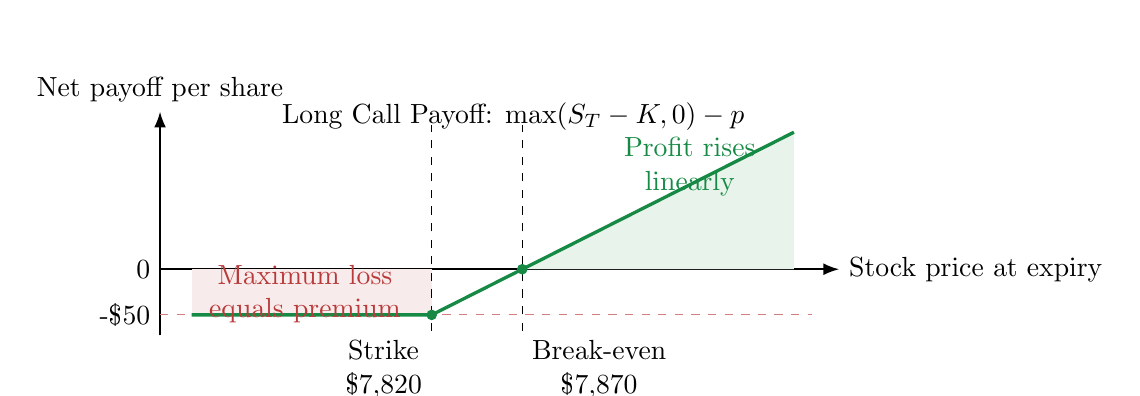
\begin{tikzpicture}[x=1.15cm,y=0.58cm,>=Latex]
    \draw[->,line width=0.6pt] (0,0) -- (7.5,0) node[right] {Stock price at expiry};
    \draw[->,line width=0.6pt] (0,-1.45) -- (0,3.45) node[above] {Net payoff per share};

    \draw[bearc!65,dashed] (0,-1) -- (7.2,-1);
    \node[left] at (0,-1) {-\$50};
    \node[left] at (0,0) {0};

    \fill[bearc!10] (0.35,0) -- (0.35,-1) -- (3,-1) -- (3,0) -- cycle;
    \fill[bullc!10] (4,0) -- (7,0) -- (7,3) -- cycle;

    \draw[dashed] (3,-1.35) -- (3,3.15);
    \draw[dashed] (4,-1.35) -- (4,3.15);
    \node[below left,align=center] at (3,-1.35) {Strike\\\$7,820};
    \node[below right,align=center] at (4,-1.35) {Break-even\\\$7,870};

    \draw[bullc,line width=1.2pt] (0.35,-1) -- (3,-1) -- (7,3);
    \filldraw[bullc] (3,-1) circle (1.7pt);
    \filldraw[bullc] (4,0) circle (1.7pt);

    \node[align=center,bearc] at (1.6,-0.55) {Maximum loss\\equals premium};
    \node[align=center,bullc] at (5.85,2.25) {Profit rises\\linearly};
    \node[align=center] at (3.9,3.35) {Long Call Payoff: \(\max(S_T-K,0)-p\)};
\end{tikzpicture}
\caption{Long call payoff with strike \$7,820 and premium \$50. The option starts making net profit only after the break-even price of \$7,870.}
\end{figure}

\begin{figure}[htbp]
\centering
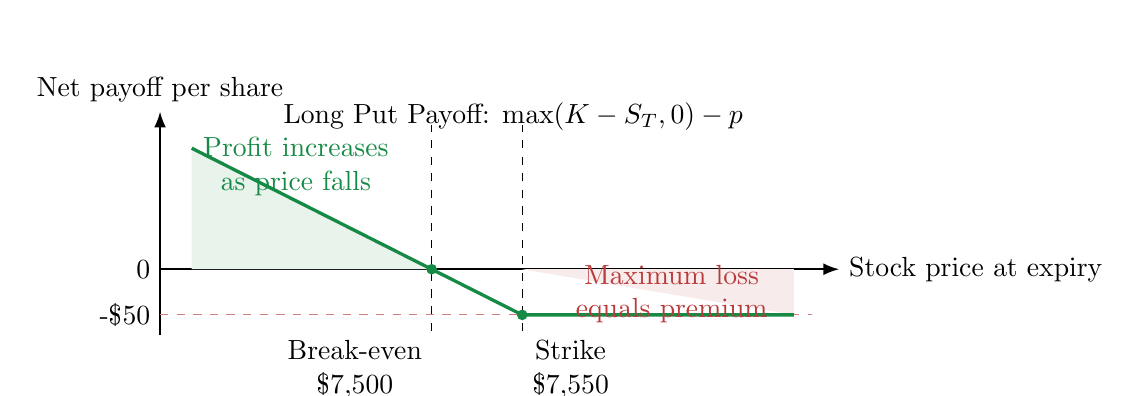
\begin{tikzpicture}[x=1.15cm,y=0.58cm,>=Latex]
    \draw[->,line width=0.6pt] (0,0) -- (7.5,0) node[right] {Stock price at expiry};
    \draw[->,line width=0.6pt] (0,-1.45) -- (0,3.45) node[above] {Net payoff per share};

    \draw[bearc!65,dashed] (0,-1) -- (7.2,-1);
    \node[left] at (0,-1) {-\$50};
    \node[left] at (0,0) {0};

    \fill[bullc!10] (0.35,0) -- (3,0) -- (0.35,2.65) -- cycle;
    \fill[bearc!10] (4,0) -- (7,-1) -- (7,0) -- cycle;

    \draw[dashed] (3,-1.35) -- (3,3.15);
    \draw[dashed] (4,-1.35) -- (4,3.15);
    \node[below left,align=center] at (3,-1.35) {Break-even\\\$7,500};
    \node[below right,align=center] at (4,-1.35) {Strike\\\$7,550};

    \draw[bullc,line width=1.2pt] (0.35,2.65) -- (3,0) -- (4,-1) -- (7,-1);
    \filldraw[bullc] (3,0) circle (1.7pt);
    \filldraw[bullc] (4,-1) circle (1.7pt);

    \node[align=center,bullc] at (1.5,2.25) {Profit increases\\as price falls};
    \node[align=center,bearc] at (5.65,-0.55) {Maximum loss\\equals premium};
    \node[align=center] at (3.9,3.35) {Long Put Payoff: \(\max(K-S_T,0)-p\)};
\end{tikzpicture}
\caption{Long put payoff with strike \$7,550 and premium \$50. The option starts making net profit only below the break-even price of \$7,500.}
\end{figure}

\FloatBarrier

\subsection{Four Positions in the Options Market}

\begin{center}
\scriptsize
\setlength{\tabcolsep}{3pt}
\begin{tabular}{|L{2.25cm}|L{2.25cm}|L{2.35cm}|L{2.7cm}|L{2.7cm}|}
\hline
\textbf{Position} & \textbf{Action} & \textbf{Market View} & \textbf{Risk} & \textbf{Reward} \\
\hline
\textbf{Long Call} & Buy a call & Bullish & Limited to premium & Theoretically unlimited \\
\hline
\textbf{Short Call} & Sell or write a call & Bearish or neutral & Theoretically unlimited & Limited to premium received \\
\hline
\textbf{Long Put} & Buy a put & Bearish & Limited to premium & Large, capped when price reaches zero \\
\hline
\textbf{Short Put} & Sell or write a put & Bullish or neutral & Large, capped when price reaches zero & Limited to premium received \\
\hline
\end{tabular}
\end{center}

\begin{quote}
\textbf{Shorting or writing an option} means taking the other side of the buyer's position. The writer receives the premium upfront but is obligated to fulfill the contract if the buyer exercises.
\end{quote}

\subsection{American vs. European Options}
\index{American option}
\index{European option}

\begin{center}
\small
\begin{tabular}{|L{3.2cm}|L{5.5cm}|L{5.5cm}|}
\hline
\textbf{Feature} & \textbf{American Option} & \textbf{European Option} \\
\hline
\textbf{Exercise} & Can be exercised any time on or before expiry & Can be exercised only on the expiry date \\
\hline
\textbf{Flexibility} & Higher, because the holder can react before expiry & Lower, because exercise is restricted to expiry \\
\hline
\textbf{Premium} & Generally higher because of added flexibility & Generally lower than an otherwise identical American option \\
\hline
\textbf{Common Usage} & Common for many single-stock options in the United States & Common for many index and stock option contracts in India \\
\hline
\end{tabular}
\end{center}

For example, a symbol such as \textbf{SBIN Oct 460 CE} refers to a State Bank of India call option with a strike price of Rs. 460 and October expiry. The suffix \textbf{CE} stands for \textbf{Call European}. Exact expiry days are exchange- and contract-specific, so traders should always check the current contract specification instead of relying on old examples.

\subsection{Exchange-Traded vs. OTC Options}
\index{Exchange-traded options}
\index{OTC options}

\begin{center}
\small
\begin{tabular}{|L{3.2cm}|L{5.5cm}|L{5.5cm}|}
\hline
\textbf{Feature} & \textbf{Exchange-Traded Options} & \textbf{OTC Options} \\
\hline
\textbf{Standardization} & Fixed contract size, strike intervals, and expiry cycles & Fully customizable terms \\
\hline
\textbf{Default Risk} & Low, because a clearinghouse stands between counterparties & Higher, because counterparty default is possible \\
\hline
\textbf{Transparency} & Publicly visible pricing, volumes, and open interest & Privately negotiated pricing and terms \\
\hline
\textbf{Liquidity} & Usually higher for active contracts & Usually lower and relationship-driven \\
\hline
\textbf{Regulation} & Heavily regulated by the exchange and market regulator & Less standardized and more dependent on bilateral agreements \\
\hline
\end{tabular}
\end{center}

The OTC options market can be larger in notional value because institutional users often need customized derivatives that cannot be found in standardized exchange-traded contracts.

\subsection{Real-World Example: Reading an Option Contract}

Consider the contract \textbf{SBIN Oct 460 CE}.

\begin{center}
\small
\begin{tabular}{|L{4cm}|L{4cm}|L{6cm}|}
\hline
\textbf{Component} & \textbf{Value} & \textbf{Meaning} \\
\hline
\textbf{SBIN} & State Bank of India & Underlying asset \\
\hline
\textbf{Oct} & October & Expiry month; the exact expiry date is defined by the exchange contract specification \\
\hline
\textbf{460} & Rs. 460 & Strike price, or the transaction price if exercised \\
\hline
\textbf{CE} & Call European & European-style call option \\
\hline
\textbf{Premium} & Rs. 17.75 per share & Price paid by the buyer and received by the seller \\
\hline
\textbf{Lot Size} & 1,500 shares & Minimum tradable contract quantity \\
\hline
\textbf{Total Premium Outflow} & Rs. \(17.75 \times 1{,}500 = 26{,}625\) & Maximum possible loss for the buyer \\
\hline
\end{tabular}
\end{center}

A call buyer at the Rs. 460 strike breaks even when SBI closes above:
\begin{equation*}
    460 + 17.75 = \text{Rs. }477.75.
\end{equation*}
If SBI closes at or below Rs. 460 on expiry, the option expires worthless and the buyer loses the total premium of Rs. 26,625.

\subsection{Key Options Jargon}
\index{Strike price}
\index{Option premium}
\index{Expiration date}
\index{Moneyness}

\begin{description}[leftmargin=!,labelwidth=4cm]
    \item[Call Option] The right to buy the underlying at the strike price. A call becomes more valuable when the underlying rises.
    \item[Put Option] The right to sell the underlying at the strike price. A put becomes more valuable when the underlying falls.
    \item[Strike Price] The predetermined price at which the option can be exercised.
    \item[Premium] The price paid by the buyer to the seller. It is non-refundable, equals the buyer's maximum loss, and equals the seller's maximum possible profit.
    \item[Expiration Date] The last date on which the option is valid. After this date, an out-of-the-money option expires worthless.
\end{description}

\subsubsection{Moneyness: ITM, OTM, and ATM}

\begin{center}
\small
\begin{tabular}{|L{3.4cm}|L{5cm}|L{5cm}|}
\hline
\textbf{Moneyness} & \textbf{Call Option} & \textbf{Put Option} \\
\hline
\textbf{In-the-Money (ITM)} & Market price \(>\) strike price & Market price \(<\) strike price \\
\hline
\textbf{Out-of-the-Money (OTM)} & Market price \(<\) strike price & Market price \(>\) strike price \\
\hline
\textbf{At-the-Money (ATM)} & Market price is approximately equal to the strike price & Market price is approximately equal to the strike price \\
\hline
\end{tabular}
\end{center}

An ATM option has little or no intrinsic value, but it can still have significant time value because the price may move favorably before expiry.

\subsubsection{Intrinsic Value and Time Value}

\textbf{Intrinsic value} is the immediate exercise value of an option. Only ITM options have positive intrinsic value:
\begin{align*}
    \text{Call Intrinsic Value} &= \max(S - K, 0), \\
    \text{Put Intrinsic Value} &= \max(K - S, 0).
\end{align*}

\textbf{Time value}, also called extrinsic value, is the part of the option premium that exceeds intrinsic value:
\begin{align*}
    \text{Premium} &= \text{Intrinsic Value} + \text{Time Value}, \\
    \text{Time Value} &= \text{Premium} - \text{Intrinsic Value}.
\end{align*}

\begin{itemize}[leftmargin=*]
    \item Time value is generally higher when more time remains until expiry.
    \item Time value decays as expiry approaches; this decay is measured by theta.
    \item Even an OTM option can have time value because it may still move ITM before expiry.
\end{itemize}

\subsubsection{Volatility}
\index{Volatility}
\index{Implied volatility}

\textbf{Volatility} measures the degree of price variation in the underlying asset. Higher volatility increases uncertainty and raises the probability that an option may finish deeply ITM, so it generally increases option premiums for both calls and puts.

\begin{center}
\small
\begin{tabular}{|L{4cm}|L{10cm}|}
\hline
\textbf{Type} & \textbf{Description} \\
\hline
\textbf{Historical Volatility (HV)} & Actual price fluctuations observed in the past. \\
\hline
\textbf{Implied Volatility (IV)} & The market's expectation of future volatility, inferred from current option prices. \\
\hline
\textbf{Realized Volatility} & The volatility that actually occurs over a measured future period. \\
\hline
\end{tabular}
\end{center}

IV is especially important for options traders because it directly affects premium levels. High IV usually means expensive options; low IV usually means cheaper options.

\subsubsection{Option Chain and Open Interest}
\index{Option chain}
\index{Open interest}

An \textbf{option chain} is a table of available contracts for an underlying asset. It usually displays strike prices, expiry dates, call premiums, put premiums, volume, and open interest.

\textbf{Open interest (OI)} is the total number of outstanding option contracts for a given strike and expiry that have not yet been closed or settled. High OI usually indicates stronger market participation and better liquidity at that strike. Traders often combine OI with price and volume to study sentiment and possible support or resistance zones.

\subsection{The Option Greeks}
\index{Option Greeks}

The Greeks measure how sensitive an option's price is to different inputs. They are the control panel of options trading.

\subsubsection{Delta \(\Delta\)}
\index{Delta}

\textbf{Delta} measures how much the option price changes for a one-unit move in the underlying asset:
\begin{equation*}
    \Delta = \frac{\partial V}{\partial S},
\end{equation*}
where \(V\) is the option value and \(S\) is the underlying price.

\begin{center}
\small
\begin{tabular}{|L{4cm}|L{4cm}|L{6cm}|}
\hline
\textbf{Option Type} & \textbf{Delta Range} & \textbf{Meaning} \\
\hline
Call Option & 0 to +1 & Call price rises as the underlying rises. \\
\hline
Put Option & -1 to 0 & Put price rises as the underlying falls. \\
\hline
\end{tabular}
\end{center}

\begin{itemize}[leftmargin=*]
    \item ATM options usually have delta near \(\pm 0.5\).
    \item Deep ITM options have delta close to \(\pm 1\), so they move almost one-for-one with the underlying.
    \item Deep OTM options have delta close to 0, so they respond weakly to small underlying moves.
\end{itemize}

Delta is also commonly used as a rough probability proxy for expiring ITM. For example, a delta of 0.30 is often interpreted as roughly a 30\% probability of expiring ITM, though this is only an approximation.

\subsubsection{Theta \(\Theta\)}
\index{Theta}

\textbf{Theta} measures the rate of time decay: how much an option's premium changes with the passage of one day, all else equal.
\begin{equation*}
    \Theta = \frac{\partial V}{\partial t}.
\end{equation*}

\begin{itemize}[leftmargin=*]
    \item Theta is usually negative for option buyers because time decay hurts long options.
    \item Theta is usually positive for option sellers because time decay benefits short options.
    \item Time decay accelerates as expiry approaches, especially for ATM options.
\end{itemize}

Theta explains why buying far OTM options with little time to expiry is risky: time decay can rapidly erode the premium even when the market does not move much.

\subsubsection{Vega \(\nu\)}
\index{Vega}

\textbf{Vega} measures how much the option price changes for a one-percentage-point change in implied volatility:
\begin{equation*}
    \nu = \frac{\partial V}{\partial \sigma},
\end{equation*}
where \(\sigma\) denotes volatility.

\begin{itemize}[leftmargin=*]
    \item Higher volatility generally increases both call and put premiums.
    \item Option buyers benefit from rising volatility and are said to be long vega.
    \item Option sellers benefit from falling volatility and are said to be short vega.
\end{itemize}

\subsubsection{Gamma \(\Gamma\)}
\index{Gamma}

\textbf{Gamma} measures the rate of change of delta for a one-unit move in the underlying. It is the acceleration of the option's price response:
\begin{equation*}
    \Gamma = \frac{\partial \Delta}{\partial S} = \frac{\partial^2 V}{\partial S^2}.
\end{equation*}

\begin{itemize}[leftmargin=*]
    \item Gamma is highest for ATM options near expiry, which makes their delta change rapidly.
    \item A high-gamma position requires more frequent hedging adjustments.
    \item Option buyers have positive gamma, while option sellers have negative gamma.
\end{itemize}

\subsubsection{Greeks Summary Table}

\begin{center}
\scriptsize
\setlength{\tabcolsep}{3pt}
\begin{tabular}{|L{2.15cm}|L{4.45cm}|L{3.05cm}|L{3.05cm}|}
\hline
\textbf{Greek} & \textbf{Measures} & \textbf{Buyer Impact} & \textbf{Seller Impact} \\
\hline
\textbf{Delta} & Price sensitivity to the underlying move & Positive for calls; negative for puts & Opposite exposure \\
\hline
\textbf{Theta} & Time decay per day & Usually negative & Usually positive \\
\hline
\textbf{Vega} & Sensitivity to implied volatility & Positive & Negative \\
\hline
\textbf{Gamma} & Rate of change of delta & Positive & Negative \\
\hline
\end{tabular}
\end{center}

\subsection{Drivers of Option Premium}

\begin{center}
\small
\begin{tabular}{|L{4.2cm}|L{4.8cm}|L{4.8cm}|}
\hline
\textbf{Driver} & \textbf{Effect on Call Premium} & \textbf{Effect on Put Premium} \\
\hline
Underlying price rises & Increases & Decreases \\
\hline
Underlying price falls & Decreases & Increases \\
\hline
Volatility increases & Increases & Increases \\
\hline
Time to expiry increases & Usually increases & Usually increases \\
\hline
Risk-free rate increases & Usually increases & Usually decreases \\
\hline
\end{tabular}
\end{center}

\begin{quote}
\textbf{Key idea:} Volatility and time are the two most important drivers of premium beyond intrinsic value. A longer-dated option is usually worth more than an otherwise similar shorter-dated option because more time creates more opportunity for the option to move ITM.
\end{quote}

\subsection{Features of Option Holders vs. Writers}

\begin{center}
\small
\begin{tabular}{|L{4.5cm}|L{5cm}|L{5cm}|}
\hline
\textbf{Feature} & \textbf{Option Buyer (Holder)} & \textbf{Option Seller (Writer)} \\
\hline
Cash flow at entry & Pays the premium upfront & Receives the premium upfront \\
\hline
Maximum profit & Unlimited for calls; large for puts & Limited to premium received \\
\hline
Maximum loss & Limited to premium paid & Unlimited for naked calls; large for naked puts \\
\hline
Exercise choice & Has the choice whether to exercise & Must fulfill the contract if exercised \\
\hline
Main risk & Time decay and wrong direction & Large adverse movement in the underlying \\
\hline
\end{tabular}
\end{center}

The asymmetry in risk and reward is the defining feature of options. Buyers pay the premium for limited downside and convex upside; writers receive the premium as compensation for accepting obligation and potentially large losses.

\subsection{Advantages and Disadvantages of Options}

\subsubsection{Advantages}

\begin{itemize}[leftmargin=*]
    \item \textbf{Insurance:} Options can protect against adverse price movements while preserving upside potential.
    \item \textbf{Lower capital requirement:} A premium can provide exposure to a much larger notional position.
    \item \textbf{Defined risk for buyers:} The maximum loss is known upfront and equals the premium paid.
    \item \textbf{Flexibility:} Strategies can be structured for rising, falling, volatile, or sideways markets.
\end{itemize}

\subsubsection{Disadvantages}

\begin{itemize}[leftmargin=*]
    \item \textbf{Time decay:} Options are wasting assets, so the premium erodes as expiry approaches.
    \item \textbf{Non-refundable premium:} The buyer loses the upfront premium if the option expires OTM.
    \item \textbf{Leverage cuts both ways:} A wrong directional bet can produce a 100\% loss of the premium paid.
    \item \textbf{Complexity:} Option prices depend on multiple interacting variables, including delta, theta, vega, gamma, time to expiry, and volatility.
\end{itemize}

\section{Going Deeper with Stock Options}


\subsection{What Is an Option Contract?}

An \textbf{option} is a legally binding contract between a buyer and a seller that gives the buyer the \textbf{right, but not the obligation}, to buy or sell an underlying asset (stock, index, currency, or commodity) at a predetermined price called the \textbf{strike price}, before or on a specific date called the \textbf{expiry date}. The critical word is "option" — the buyer has a \emph{choice}, not a compulsion. The seller, by contrast, has an \emph{obligation} if the buyer chooses to act.

Options were originally designed to \textbf{manage risk}. Depending on how they are used — as a hedge, a speculative instrument, or portfolio insurance — they serve different purposes. What is important is that risk is being \textbf{transferred} from one party to another each day in the options market.

The two parties to every options contract are:

\begin{itemize}[leftmargin=*]
    \item \textbf{Option Buyer (Holder):} Pays a premium upfront to acquire the right. Can choose to exercise or walk away.
    \item \textbf{Option Seller / Writer:} Receives the premium. Has no choice — must fulfil the contractual obligation if the buyer exercises.
\end{itemize}


\subsection{Types of Options}

\subsubsection{Call Options}

A \textbf{call option} gives the buyer the right (but not the obligation) to \textbf{buy} the underlying asset at the agreed strike price on or before expiry. The buyer profits when the underlying price rises above the strike price.

\begin{quote}
\textbf{The Coupon Analogy:} Think of a call option like a restaurant coupon offering a roast beef combo for \$3.99 (the strike price) expiring on April 30 (the expiry date). If the combo currently costs \$5 on the menu (market price), you use the coupon — you exercise your right to buy below market price. But if the combo has fallen to \$2.99 in the market, you simply ignore the coupon and buy at the cheaper market price. The coupon isn't useful, but it also costs you nothing extra — your only loss is the initial price of the coupon (the premium). This is precisely how a call option works.
\end{quote}

\subsubsection{Put Options}

A \textbf{put option} gives the buyer the right (but not the obligation) to \textbf{sell} the underlying asset at the strike price on or before expiry. The buyer profits when the underlying price falls below the strike price.

\begin{center}
\scriptsize
\setlength{\tabcolsep}{3pt}
\begin{tabular}{|L{4.40cm}|L{4.40cm}|L{4.40cm}|}
\hline
Option Type & Buyer's Right & Buyer Profits When \\
\hline
\textbf{Call} & Buy at strike price & Underlying price rises above strike \\
\hline
\textbf{Put} & Sell at strike price & Underlying price falls below strike \\
\hline
\end{tabular}
\end{center}

\subsection{Core Option Jargons}

\subsubsection{Strike Price (Exercise Price)}

The \textbf{strike price} is the pre-agreed anchor price at which the buyer and seller agree to transact. For a call option, it is the price at which the buyer may purchase the underlying stock at expiry. For a put, it is the price at which the buyer may sell.

For example, if you buy ITC's 340 Call option, you are paying a premium today to secure the \textbf{right to buy ITC shares at ₹340 on the expiry date}. You would exercise this right only if ITC trades above ₹340 on expiry — otherwise the right has no value.

Multiple strike prices exist simultaneously for every underlying (e.g., ₹260, ₹270, ₹280 ... ₹480 for ITC in ₹10 intervals). Each strike is an independent contract with its own premium. All available strikes for a given underlying and expiry are displayed together in what is called the \textbf{Option Chain}.

\subsubsection{Underlying Price}

The \textbf{underlying price} is the current market price of the asset (stock or index) on which the option is written. Options derive their value from this price — as a derivative, their worth changes as the underlying moves. For a call option buyer to profit, the underlying price must rise above the strike. If ITC trades at ₹336.90 in the spot market, that is the underlying price.

\subsubsection{Option Premium}

The \textbf{premium} is the price paid by the option buyer to the option seller/writer in exchange for the rights conferred by the contract. It is paid upfront at the time of entering the trade. For the buyer, the premium represents the \textbf{maximum possible loss}. For the seller, it is the income received and the \textbf{maximum possible profit}.

\textbf{Premium is not fixed — it fluctuates continuously}, often minute by minute in live markets. Two intuitive factors that influence premium are:

\begin{itemize}[leftmargin=*]
    \item \textbf{Event Risk / Uncertainty:} When a significant corporate or market event is anticipated (quarterly earnings, policy decisions, elections), the probability of a large price move increases. A seller facing this uncertainty demands higher compensation. When no such event is in sight, sellers accept lower premiums. A seller who knows the odds are stacked in their favour (speculative news, remote chance of the event materialising) may accept a modest premium; the same seller will demand far more if an outcome looks more probable.
\end{itemize}

\begin{itemize}[leftmargin=*]
    \item \textbf{Time to Expiry:} More time remaining = more opportunity for the underlying to move in the buyer's favour = higher premium. As expiry approaches and time shrinks, this "time value" component of the premium erodes continuously. This erosion is called \textbf{time decay} (governed by the Greek \textbf{Theta}). A buyer with 6 months to expiry would pay significantly more premium than a buyer with only 10 days remaining, because the shorter timeframe dramatically reduces the probability of a favourable move.
\end{itemize}

In totality, five specific factors — collectively known as the \textbf{Option Greeks} (Delta, Gamma, Theta, Vega, Rho) — govern premium behaviour. They are studied in detail in later chapters.

\subsubsection{Exercising an Option}

\textbf{Exercising an option} means claiming your contractual right — the act of demanding to buy (call) or sell (put) the stock at the agreed strike price. In Indian equity markets, options follow the \textbf{European style}, meaning they can only be exercised \textbf{on the day of expiry}, not before. This is a critical distinction.

\begin{quote}
\textbf{Example:} You buy ITC's 340 Call option with 15 days to expiry when ITC is trading at ₹330. The very next day, ITC jumps to ₹360. Despite the favourable move, you \textbf{cannot demand settlement yet} — the right to exercise exists only on the expiry date. However, you can \textbf{sell your option contract in the secondary market} at any time before expiry to lock in your profit (the premium will have risen significantly due to the favourable price move). The act of selling back the contract is \textbf{not} exercising — it is simply closing your position.
\end{quote}

\textbf{American vs. European Style:}
\begin{itemize}[leftmargin=*]
    \item \textbf{American-style options} can be exercised at \textbf{any time before expiry}. Individual US equity options fall into this category.
    \item \textbf{European-style options} can only be exercised \textbf{on the expiry date}. Indian equity and index options fall here.
    \item Both styles allow you to \textbf{close your position} (sell the contract back to the market) before expiry — the distinction only matters for the act of \emph{exercising} (converting to the physical stock).
\end{itemize}

\subsubsection{Option Expiry}

Options contracts, like futures, have a defined expiry date after which the contract ceases to exist. In India:

\begin{itemize}[leftmargin=*]
    \item \textbf{Equity and Index Options} expire on the \textbf{last Thursday of every month} (for monthly contracts). Weekly contracts on indices like Nifty expire every Thursday.
    \item Three monthly series are always active: \textbf{Current Month, Mid Month (next month), and Far Month} (the month after).
    \item Premiums differ across expiry dates — longer-dated options carry higher premiums because more time means a greater chance of profitable moves.
\end{itemize}

\begin{quote}
\textbf{Example:} An Ashok Leyland 70 Call option might have three choices — 26th March (current), 30th April (mid), and 28th May (far month), each with its own distinct premium.
\end{quote}

For American-style index options (relevant for global markets): the last trading day is typically the \textbf{third Friday of the expiry month} (or the preceding Thursday if that Friday is a market holiday). Technical expiry is the \textbf{Saturday immediately following the third Friday}. Always verify expiry dates, especially around public holidays.

\subsubsection{Option Settlement}

In India, equity options are \textbf{cash settled}, meaning that no actual delivery of shares occurs. Instead, only the \textbf{cash equivalent of the profit or loss} is transferred on expiry day.

\begin{quote}
\textbf{Detailed Example:} Trader A buys JP Associates' 25 Call option (market lot: 8,000 shares) by paying ₹1.35 × 8,000 = \textbf{₹10,800} as premium to Trader B. On expiry, JP Associates trades at ₹32 in the spot market.

Normally, this would mean:
\begin{itemize}[leftmargin=*]
    \item Trader A has the right to buy 8,000 shares at ₹25 = pays ₹2,00,000
    \item Trader A sells those shares in the open market at ₹32 = receives ₹2,56,000
    \item Gross profit = ₹56,000
\end{itemize}

Since options are cash settled, Trader B simply pays Trader A the cash equivalent:
\begin{itemize}[leftmargin=*]
    \item Cash settlement = (32 − 25) × 8,000 = ₹56,000
    \item Trader A's net profit = ₹56,000 − ₹10,800 (premium paid) = \textbf{₹45,200}
    \item Percentage return on capital deployed = 45,200 / 10,800 ≈ \textbf{419\%}
\end{itemize}
\end{quote}

This asymmetric return profile — small upfront capital outlay for potentially enormous gains — is the defining attraction of options. A move from ₹25 to ₹32 (a 28\% rise in the underlying) translates into a 419\% return on the option premium. This is the power of leverage embedded in options.


\subsection{Option Moneyness: ITM, ATM, OTM}

\textbf{Moneyness} describes the relationship between the current underlying price and an option's strike price. It determines whether an option has intrinsic value right now. Traders use three categories, commonly abbreviated:

\subsubsection{For Call Options:}

\begin{center}
\scriptsize
\setlength{\tabcolsep}{3pt}
\begin{tabular}{|L{4.40cm}|L{4.40cm}|L{4.40cm}|}
\hline
Moneyness & Condition & Meaning \\
\hline
\textbf{In the Money (ITM)} & Underlying Price > Strike Price & Has intrinsic value; would be profitable to exercise right now \\
\hline
\textbf{At the Money (ATM)} & Underlying Price ≈ Strike Price & On the boundary; no intrinsic value, pure time value \\
\hline
\textbf{Out of the Money (OTM)} & Underlying Price < Strike Price & No intrinsic value; stock must rally for the option to profit \\
\hline
\end{tabular}
\end{center}

\subsubsection{For Put Options:}

\begin{center}
\scriptsize
\setlength{\tabcolsep}{3pt}
\begin{tabular}{|L{4.40cm}|L{4.40cm}|L{4.40cm}|}
\hline
Moneyness & Condition & Meaning \\
\hline
\textbf{In the Money (ITM)} & Underlying Price < Strike Price & Has intrinsic value; can sell above current market price \\
\hline
\textbf{At the Money (ATM)} & Underlying Price ≈ Strike Price & On the boundary \\
\hline
\textbf{Out of the Money (OTM)} & Underlying Price > Strike Price & No intrinsic value; stock must fall for the option to profit \\
\hline
\end{tabular}
\end{center}

\subsubsection{Option Premium Composition}

\begin{quote}
\textbf{Premium = Intrinsic Value + Extrinsic Value (Time Value)}
\end{quote}

\begin{itemize}[leftmargin=*]
    \item \textbf{Intrinsic Value:} The immediate exercisable profit. Only ITM options have intrinsic value (e.g., a 340 Call when the stock is at ₹360 has ₹20 of intrinsic value). ATM and OTM options have zero intrinsic value.
    \item \textbf{Extrinsic / Time Value:} The remaining portion of the premium, reflecting the time left to expiry and the implied volatility. Even an OTM option has positive premium as long as time remains — there is still a chance for the stock to move in your favour.
\end{itemize}

As expiry approaches, the extrinsic value approaches zero, and OTM options eventually expire worthless. Deep OTM options appear attractively cheap but are priced that way because their probability of becoming profitable is very low. Cheap ≠ good value.


\subsection{Contract Multipliers and Lot Size}

Options contracts are \textbf{standardised} — they have fixed strike price intervals, set expiry dates, and defined contract (lot) sizes. This standardisation was introduced to ensure market liquidity and operational efficiency.

\textbf{The Core Rule:} One option contract controls a fixed number of shares — the \textbf{contract multiplier} or \textbf{lot size}. In US markets this is universally \textbf{100 shares per contract}. In Indian markets, lot sizes vary by underlying (e.g., Nifty 50 Index Options have a lot size of 75; individual stocks have their own defined lot sizes).

When a premium is quoted as ₹4.75 or \$18.80, this is the per-share (per-unit) price. The actual cost to enter one contract is:

\begin{quote}
\textbf{Contract Cost = Premium per Unit × Lot Size}
\end{quote}

So if a Nifty option is priced at ₹100 and the lot size is 75, buying one contract costs ₹7,500, not ₹100.

At expiry, if you exercise one option contract, your right applies to the \textbf{full lot of shares} at the strike price. Always confirm the lot size before placing a trade — it directly determines your total exposure.


\subsection{Options vs. Stock Trading}

\subsubsection{Why Stocks Are Popular}

Before understanding the advantages of options, it helps to understand why most investors begin with stocks:

\begin{enumerate}[leftmargin=*]
    \item \textbf{Single-dimensional, easy to understand:} You get the direction right, you profit. Buy low, sell high — or short-sell and cover lower.
    \item \textbf{Easy to purchase:} The concept has been reinforced for decades and is universally familiar.
    \item \textbf{Time flexibility:} Stock positions can be held for years or decades, giving a losing trade time to recover without being forced out.
    \item \textbf{Perceived safety:} Widely accepted as the standard form of investing; mainstream media treats stock investing as inherently safe.
\end{enumerate}

These are valid reasons, but they do not necessarily make stocks the \emph{best} vehicle for deploying capital.

\subsubsection{The Fundamental Problem: Markets Are Random}

The stock market follows a \textbf{normal (random) distribution}. This is not an opinion — it has been proven statistically:

\begin{itemize}[leftmargin=*]
    \item \textbf{68\% of all price moves} in a given period fall within one standard deviation of the current price.
    \item In the tails of the distribution are the anomalies — extreme up or down moves — but these are rare.
    \item The central implication: on any given trade, a stock has essentially a \textbf{50\% chance of going up and a 50\% chance of going down}. It is a fair game.
\end{itemize}

This randomness extends to professional forecasters as well. A study covering the top 14 investment firms' market return predictions from 2006 onward found:

\begin{itemize}[leftmargin=*]
    \item Average predicted annual return: \textbf{10.32\%}
    \item Actual S\&P 500 average annual return: \textbf{4.76\%}
    \item The professionals were consistently \textbf{off by over 100\%} in their estimates — and yet their fees remained unchanged.
\end{itemize}

The 50-year historical average return of the S\&P 500 is 6.26\%. Rather than using that as a baseline, these highly paid analysts consistently predicted double, and they were wrong year after year.

\textbf{The conclusion:} If you knew nothing about where the market was headed (50/50 odds), and you add commission costs on every trade, making consistent long-term profits through stock direction trading becomes extremely difficult. Neither you nor anyone else reliably knows where the market is going.

\subsubsection{Why Options Are Superior}

Because options are built around \textbf{probabilities} rather than pure direction, they offer structural advantages:

\begin{enumerate}[leftmargin=*]
    \item \textbf{Multiple ways to profit:} With stocks, you only profit if the price goes in your predicted direction. With options, you can design strategies that profit when the stock goes up, down, or even stays flat (sideways). Volatility and time decay become additional profit engines independent of direction.
\end{enumerate}

\begin{enumerate}[leftmargin=*]
    \item \textbf{Known probabilities upfront:} Before entering any trade, you can calculate the \textbf{exact probability of success} for your chosen strike and strategy. An iron condor might have a 70\% probability of full profit — you know this before you deploy a single rupee. No stock trade offers this transparency.
\end{enumerate}

\begin{enumerate}[leftmargin=*]
    \item \textbf{Leverage:} One option contract controls 100 shares (or one lot). Instead of buying 100 shares of a \$50 stock (\$5,000 outlay), you could buy one deep ITM call option for \textasciitilde{}\$510 and participate in the same price movement. Capital efficiency is dramatically improved.
\end{enumerate}

\begin{enumerate}[leftmargin=*]
    \item \textbf{Third-dimension factors (Volatility and Time Decay):} Options pricing incorporates implied volatility and time decay, which are independent of direction. A skilled options seller can profit simply from the passage of time (theta decay) without needing the stock to move at all. Strategies like iron condors, credit spreads, covered calls, and strangles are built entirely around this.
\end{enumerate}

\begin{enumerate}[leftmargin=*]
    \item \textbf{Defined and controlled risk:} Option buyers have a hard floor on their losses — the maximum they can lose is the premium paid, no matter how badly the underlying moves against them. This defined risk is impossible with outright stock or futures positions.
\end{enumerate}


\subsection{Smart Use of Leverage and Risk Management}

Leverage is the most powerful feature of options — and the most dangerous if misused. The principle is simple: instead of deploying ₹5,00,000 in shares, you control the same economic exposure with ₹50,000 in options premium. The return on capital is multiplied. But so are the losses if the trade goes wrong.

\textbf{The Risk of Overleveraging — A Mathematical Reality:}

When you lose money, you need a proportionally \emph{larger} gain to recover. This is not simple addition:

\begin{center}
\scriptsize
\setlength{\tabcolsep}{3pt}
\begin{tabular}{|L{3.30cm}|L{3.30cm}|L{3.30cm}|L{3.30cm}|}
\hline
Starting Balance & Loss \% & Remaining & Recovery Required \\
\hline
₹10,000 & 25\% & ₹7,500 & \textbf{33.3\%} \\
\hline
₹10,000 & 50\% & ₹5,000 & \textbf{100\%} \\
\hline
₹10,000 & 75\% & ₹2,500 & \textbf{300\%} \\
\hline
₹10,000 & 90\% & ₹1,000 & \textbf{900\%} \\
\hline
\end{tabular}
\end{center}

After losing 25\%, you need a 33\% gain just to get back to where you started — not 25\%. Many newsletters falsely show "lost 25\%, gained 30\% = up 5\%" — this arithmetic is wrong because the 30\% gain is on a smaller base. This misrepresentation is common and misleading.

\textbf{The Recommended Allocation Rule:} Never risk more than \textbf{1\% to 5\% of your total account per trade}. At this scale, no single bad trade can meaningfully damage your overall capital. If you follow this rule, it is practically impossible to "blow up" your account — the mathematical floor is always preserved.


\subsection{Profit and Loss (P\&L) Diagrams}

P\&L diagrams (also called payoff diagrams) are \textbf{visual representations} of how much money an options strategy makes or loses at different underlying prices — either today or at expiry. Mastering these diagrams is essential because they instantly reveal:

\begin{itemize}[leftmargin=*]
    \item The \textbf{break-even price} (where the strategy crosses from loss to profit)
    \item The \textbf{maximum profit} and where it is achieved
    \item The \textbf{maximum loss} and where it is capped or open-ended
    \item The full profit/loss profile across all possible stock prices
\end{itemize}

\textbf{Structure of a P\&L Diagram:}
\begin{itemize}[leftmargin=*]
    \item \textbf{Horizontal axis (X):} Stock / underlying price
    \item \textbf{Vertical axis (Y):} Profit or loss (₹ amount)
    \item \textbf{Zero line:} The horizontal line representing break-even (neither profit nor loss)
    \item \textbf{Strategy line (solid/green):} The P\&L at expiry for each possible stock price
    \item \textbf{Current P\&L line (dotted/purple):} The P\&L today, before expiry. The gap between today's line and the expiry line represents the \textbf{time value} and \textbf{implied volatility value} remaining in the position.
\end{itemize}

\begin{quote}
\textbf{Practical Example (Short Strangle on XOP):} An XOP short strangle sold with a 26 Put and a 35 Call (both short). The P\&L diagram shows a profit plateau between ₹26 and ₹35. As long as XOP stays within this band at expiry, the maximum profit of \textasciitilde{}\$164 is achieved. If XOP moves to \$37, the loss is approximately \$200. The "purple" today line shows the current unrealised P\&L, while the "green" expiry line shows what happens if the position is held to expiry. At a current stock price of \$30.77, the position is already showing \textasciitilde{}\$94 of profit today, with another \$64 available if held to expiry.
\end{quote}

\textbf{P\&L shapes of common strategies:}
\begin{itemize}[leftmargin=*]
    \item \textbf{Long Call:} Flat loss (capped at premium) below strike; unlimited upside above break-even.
    \item \textbf{Short Call:} Flat profit (capped at premium received) below strike; unlimited losses above.
    \item \textbf{Long Put:} Flat loss (capped at premium) above strike; growing profit as stock falls.
    \item \textbf{Short Put:} Flat profit (capped at premium received) above strike; growing loss below break-even.
    \item \textbf{Iron Condor:} A "tent" shape — maximum profit in the middle range between two strike pairs, capped losses on both tails.
    \item \textbf{Bullish Call Debit Spread:} Limited profit, limited loss — the debit paid is the max loss; the spread width minus the debit is the max gain.
\end{itemize}

\subsection{Basic Option Strategies}

\subsubsection{Long Call Option}

\textbf{Market Outlook:} Strongly \textbf{bullish} — you expect the stock to rise significantly beyond the strike price before expiry.

\textbf{Setup:} Buy one call option at your desired strike and expiry. The further OTM the strike, the more bullish the stance (and the cheaper but less probable the option).

\textbf{Risk \& Reward:}
\begin{itemize}[leftmargin=*]
    \item \textbf{Maximum Loss:} Limited to the \textbf{premium paid} — fixed and known upfront.
    \item \textbf{Maximum Profit:} Theoretically \textbf{unlimited} (stock can rise infinitely).
    \item \textbf{Break-even at Expiry:} Strike Price + Premium Paid
\end{itemize}

\begin{quote}
\textbf{Example:} Stock at ₹40. Buy one 40 Call for ₹200. Break-even = ₹42. If stock closes at ₹55 at expiry, profit = (55 − 40 − 2) × 100 = ₹1,300. If stock closes at ₹38, the option expires worthless and you lose ₹200.
\end{quote}

\textbf{Effect of Volatility:} Rising implied volatility \textbf{helps} — increases the option's value.

\textbf{Effect of Time Decay:} \textbf{Hurts} the buyer. The option loses value every day without a favourable move. The stock must move decisively.

\textbf{Best Practices:}
\begin{itemize}[leftmargin=*]
    \item For speculation, focus on \textbf{at-the-money or slightly OTM} strikes. These offer the best balance of cost vs. responsiveness.
    \item Deep OTM options look cheap but have very low probability — avoid for speculation.
    \item For hedging an existing short position, OTM calls are appropriate (cheaper, further from the money).
\end{itemize}


\subsubsection{Short Call Option (Naked Call)}

\textbf{Market Outlook:} \textbf{Neutral to bearish} — you expect the stock to stay flat or fall, and believe a significant rally is remote.

\textbf{Setup:} Sell (write) one call option, typically \textbf{out of the money}, and collect the premium as immediate income.

\textbf{Risk \& Reward:}
\begin{itemize}[leftmargin=*]
    \item \textbf{Maximum Profit:} Limited to the \textbf{premium received} — collected at trade initiation.
    \item \textbf{Maximum Loss:} Theoretically \textbf{unlimited} — if the stock rallies without bound, losses grow indefinitely.
    \item \textbf{Break-even at Expiry:} Strike Price + Premium Received
\end{itemize}

\begin{quote}
\textbf{Example:} Stock at ₹48. Sell one 50 Call for ₹300. As long as the stock stays below ₹50 at expiry, the option expires worthless and you keep all ₹300. If the stock rises to ₹65, you face a loss of (65 − 50 − 3) × 100 = ₹1,200.
\end{quote}

\textbf{Effect of Volatility:} \textbf{Harmful} — rising volatility increases the option's value (your liability) and the probability of a damaging move.

\textbf{Effect of Time Decay:} \textbf{Beneficial} — every day without the stock moving above the strike adds to your realised gain.

\textbf{Critical Caution:} Never write naked calls on \textbf{individual stocks} — single stocks can gap up 30–50\% overnight on buyout news or surprise earnings. This risk is catastrophic. Apply this strategy on \textbf{indices and broad commodities} where such extreme discrete jumps are far less likely. Preferred parameters: sell deep OTM calls with 90–95\% historical probability of expiry worthless.


\subsubsection{Long Put Option}

\textbf{Market Outlook:} \textbf{Bearish} — you expect the stock to fall below the strike price. Unlike short-selling shares directly (which carries unlimited upside risk), a long put \textbf{caps your loss at the premium paid}.

\textbf{Setup:} Buy one put option at your desired strike and expiry. The further OTM, the more bearish and the cheaper (but less probable) the position.

\textbf{Risk \& Reward:}
\begin{itemize}[leftmargin=*]
    \item \textbf{Maximum Loss:} Limited to the \textbf{premium paid}.
    \item \textbf{Maximum Profit:} Theoretically limited only by the stock falling to zero. For a ₹40 stock with a 40 Put, maximum profit = (40 − 0 − premium paid) × lot size.
    \item \textbf{Break-even at Expiry:} Strike Price − Premium Paid
\end{itemize}

\begin{quote}
\textbf{Example:} Stock at ₹40. Buy one 40 Put for ₹200. Break-even = ₹38. If stock falls to ₹25 at expiry, profit = (40 − 25 − 2) × 100 = ₹1,300. If stock stays at ₹40 or rises, the option expires worthless and you lose ₹200.
\end{quote}

\textbf{Effect of Volatility:} \textbf{Helpful} — rising volatility increases put values. Even better: falling markets typically trigger rising volatility, creating a double boost for long put holders.

\textbf{Effect of Time Decay:} \textbf{Harmful} — time value erodes daily. The stock must fall before expiry.

\textbf{Best Uses:}
\begin{itemize}[leftmargin=*]
    \item \textbf{Hedging:} Deep OTM puts are cheap portfolio insurance for an existing long portfolio. Like buying fire insurance for your house — you pay a premium and hope never to need it.
    \item \textbf{Speculation on downside:} ATM or slightly OTM puts offer better probability for directional bearish bets.
\end{itemize}

\subsubsection{Short Put Option (Naked Put / Cash-Secured Put)}

\textbf{Market Outlook:} \textbf{Neutral to bullish} — you expect the stock to stay flat or rise, and believe a major decline is unlikely.

\textbf{The Insurance Analogy:} Selling a put is exactly like being an insurance company. You collect a premium from the buyer to protect them from losses below the strike price. If the stock never falls to the strike, you keep the entire premium — exactly as an insurer keeps premiums when no claim is filed.

\textbf{Setup:} Sell one put option, typically \textbf{out of the money}, and collect the premium immediately.

\textbf{Risk \& Reward:}
\begin{itemize}[leftmargin=*]
    \item \textbf{Maximum Profit:} Limited to the \textbf{premium received}.
    \item \textbf{Maximum Loss:} Large but technically limited — the worst case is the stock falling to zero. You are obligated to buy the stock at the strike price even if it is now worthless.
    \item \textbf{Break-even at Expiry:} Strike Price − Premium Received
\end{itemize}

\begin{quote}
\textbf{Example:} Stock at ₹50. Sell one 45 Put for ₹200. As long as the stock stays above ₹45 at expiry, the option expires worthless and you keep ₹200. Break-even = ₹43. If the stock falls to ₹30, your loss = (45 − 30 − 2) × 100 = ₹1,300.
\end{quote}

\textbf{Effect of Volatility:} \textbf{Harmful} — rising volatility makes option prices rise, increasing your liability.

\textbf{Effect of Time Decay:} \textbf{Beneficial} — every day without the stock falling moves you closer to maximum profit.

\textbf{Profit-Taking Tip:} If you sold the put for ₹200 and it has decayed to ₹100 mid-cycle, you can buy it back for ₹100, locking in ₹100 profit early and freeing your capital. You do not need to hold to expiry.

\textbf{Best Practices:}
\begin{itemize}[leftmargin=*]
    \item Sell \textbf{deep OTM puts} — 20–30\% below the current stock price — with 90–95\% historical probability of expiring worthless.
    \item Prefer \textbf{indices and commodities} over individual stocks to avoid catastrophic gap-down risk.
    \item This is widely considered among the most consistent income-generating strategies when applied correctly.
\end{itemize}

\subsection{What Is an Option Chain?}

An \textbf{option chain} is a comprehensive, tabular display of \textbf{all available option contracts} — both calls and puts — for a specific underlying asset across all available strike prices for a given expiry. It is the single most important tool for options analysis, condensing an enormous amount of market intelligence into one structured view.

\textbf{Where to find it:} Broker platforms (Zerodha, Sensibull), NSE/BSE websites, Yahoo Finance, Google Finance, and MoneyControl all provide option chains — real-time or with slight delay.

\textbf{Structure of a Typical Option Chain:}


\begin{center}
\scriptsize
\setlength{\tabcolsep}{5pt}
\renewcommand{\arraystretch}{1.2}
\begin{tabular}{|c|c|c|c|c|}
\hline
\multicolumn{2}{|c|}{\textbf{Calls Data}} & \textbf{Strike Price} & \multicolumn{2}{c|}{\textbf{Puts Data}} \\
\hline
\textbf{OI} & \textbf{Premium} & \textbf{Centre column} & \textbf{Premium} & \textbf{OI} \\
\hline
High call interest & Call price & \textbf{ATM highlighted} & Put price & High put interest \\
\hline
\end{tabular}
\end{center}


\begin{itemize}[leftmargin=*]
    \item \textbf{Call options} data is on the \textbf{left}
    \item \textbf{Strike prices} run down the \textbf{centre}
    \item \textbf{Put options} data is on the \textbf{right}
    \item The \textbf{ATM strike} (closest to current spot price) is typically highlighted
\end{itemize}

\subsection{Components of the Option Chain (Detailed)}

\subsubsection{Contract Name}
A unique identifier for each contract — specifies the underlying, strike, option type (CE = Call European, PE = Put European), and expiry date. Used for identification and order placement.

\subsubsection{Strike Price}
The pre-agreed transaction price. Strike prices are listed at standardised intervals (e.g., every ₹50 for Nifty, every ₹10 for mid-cap stocks). The strike closest to the current spot price is the \textbf{At-the-Money (ATM)} strike.

\subsubsection{Last Traded Price (LTP) / Premium}
The most recent price at which the option contract traded. This is the current \textbf{market premium} of the option. It changes continuously during market hours.

\subsubsection{Change and \% Change}

\begin{itemize}[leftmargin=*]
    \item \textbf{Change:} LTP (today) − LTP (previous session). Positive = premium has risen; Negative = premium has fallen.
    \item \textbf{\% Change:} (Change / Previous LTP) × 100. Shows the magnitude of the move in percentage terms.
\end{itemize}

\subsubsection{Bid Price and Ask Price}

\begin{itemize}[leftmargin=*]
    \item \textbf{Bid Price:} The highest price any buyer is currently willing to pay. If buyer A offers ₹50 and buyer B offers ₹55, buyer B's ₹55 is at the top of the bid — they have priority.
    \item \textbf{Ask Price:} The lowest price any seller is currently willing to accept. If seller X asks ₹55 and seller Y asks ₹50, seller Y's ₹50 is at the top of the ask — they get matched first.
    \item \textbf{Bid-Ask Spread:} The difference between the best bid and best ask. A \textbf{wide spread signals low liquidity} — fewer participants, harder to trade efficiently. A narrow spread signals high liquidity. Always check the spread before trading less popular strikes or stocks.
\end{itemize}

\subsubsection{Volume}

\textbf{Volume} is the \textbf{total count of contracts that have changed hands} (bought and sold) during the current trading day. Every single transaction — whether it opens a new position or closes an old one, whether between existing or new participants — contributes to volume.

\textbf{Key Properties of Volume:}
\begin{itemize}[leftmargin=*]
    \item \textbf{Always increases} throughout the trading day. It resets to zero at the start of each new session.
    \item Does NOT distinguish between new position creation and position closure — every trade adds to the count.
    \item High volume = high liquidity and trading interest in that contract.
    \item Low volume = fewer participants, potential difficulty entering or exiting positions cleanly.
\end{itemize}

\begin{quote}
\textbf{Volume Example (cumulative over 4 days):}
\begin{itemize}[leftmargin=*]
    \item Day 1: A buys 1 from B → Volume = 1
    \item Day 2: C buys 3 from D → Volume = 4
    \item Day 3: A sells 1 back to D (existing parties closing) → Volume = 5
    \item Day 4: C sells 3 to E (new buyer, position transfer) → Volume = 8
\end{itemize}
Volume kept growing regardless of whether positions were new or closing.
\end{quote}

\subsubsection{Open Interest (OI)}

\textbf{Open Interest} is the \textbf{total number of outstanding contracts that currently exist in the market} — contracts that have been opened but not yet closed, expired, or exercised. It reflects the total number of \emph{active} positions on each side of the market at any given moment.

\textbf{How Open Interest Changes — The Three Rules:}

Understanding OI requires knowing exactly when it goes up, down, or stays the same:

\textbf{Rule 1 — OI Increases:} When \textbf{two new participants} enter the market and create a contract (one new buyer + one new seller), a brand-new contract is born. OI increases by 1.

\textbf{Rule 2 — OI Decreases:} When \textbf{two existing participants} close their positions against each other (an existing buyer sells back to an existing seller who buys back), the contract is extinguished. OI decreases by 1.

\textbf{Rule 3 — OI Unchanged:} When an \textbf{existing participant transfers their position to a new participant} (e.g., an existing buyer sells their contract to a brand-new buyer entering the market), ownership changes but the total number of open contracts does not. OI stays the same — it is merely a position transfer, not creation or destruction.

\begin{quote}
\textbf{Detailed OI Walkthrough:}

\emph{Day 1:} Trader A buys 1 contract from Trader B (both new) → OI = \textbf{1}

\emph{Day 2:} Trader C buys 3 contracts from Trader D (both new, A's contract still open) → OI = \textbf{4}

\emph{Day 3:} Trader A (existing buyer) sells 1 contract back to Trader D (existing seller) → both close their position → OI = \textbf{3} (one contract destroyed)

\emph{Day 4:} Trader C (existing buyer of 3) sells all 3 to new Trader E → OI = \textbf{3} (unchanged — position just transferred from C to E)
\end{quote}

This walkthrough shows that OI can go up (new creation), down (existing parties close), or stay flat (transfer). \textbf{Volume in the same period kept increasing at every step}, independent of what happened to OI.

\textbf{OI and Liquidity:} High OI at a given strike means many participants hold positions there — it is easy to enter and exit. Low OI means thin participation. Always compare OI across strikes and across different underlying assets before choosing where to trade. Nifty 50's ATM OI of 10 lakh contracts vs. a small-cap stock's ATM OI of 20,000 contracts tells you where the liquidity lies.

\subsubsection{Change in OI (OI Change)}

The difference between today's OI and the previous session's OI. Displayed visually:
\begin{itemize}[leftmargin=*]
    \item \textbf{Green / Positive:} OI has \textbf{increased} → new positions are being created.
    \item \textbf{Red / Negative:} OI has \textbf{decreased} → positions are being closed.
\end{itemize}

\begin{quote}
\textbf{Example:} Nifty 25900 CE shows OI = 90 lakh with a +51\% OI change (green). This means 90 lakh contracts are currently open on this strike, and yesterday there were roughly 60 lakh — an additional 30 lakh contracts have been freshly created. Meanwhile, the 26200 PE shows a red OI change — participants are exiting that strike and potentially moving their exposure elsewhere.
\end{quote}

\subsubsection{Implied Volatility (IV)}

The market's \textbf{forward-looking expectation of volatility}, derived from the current option premium using an options pricing model. Higher IV means the market expects larger price swings. IV for each strike is visible in the "Greeks" view of most option chains. \textbf{ATM IV} is particularly important — it is the market's overall fear/confidence gauge. High IV = expensive premiums (good time to sell). Low IV = cheap premiums (good time to buy). When IV spikes dramatically, it typically signals panic or uncertainty.

\subsubsection{Put-Call Ratio (PCR)}

\textbf{PCR = Total Put OI / Total Call OI} (or sometimes calculated using volume). It is a market sentiment barometer:

\begin{itemize}[leftmargin=*]
    \item \textbf{PCR > 1:} More puts outstanding than calls — participants are collectively more bearish or hedged.
    \item \textbf{PCR < 1:} More calls outstanding — bullish positioning is dominant.
    \item \textbf{PCR around 0.7–0.8:} Considered balanced or mildly bullish in Indian markets.
\end{itemize}

PCR is most useful as a contrarian indicator at extremes — extremely high PCR can signal excessive bearishness (a potential bounce), while extremely low PCR can signal complacency (potential correction).

\subsubsection{Max Pain}

\textbf{Max Pain} is the strike price at which the \textbf{total value of all outstanding options (both calls and puts) expires at the lowest aggregate payout to option buyers} — equivalently, option sellers collectively make the most money at this price. It is calculated by summing up the total monetary pain inflicted on buyers at each possible strike price and identifying the minimum.

The theory behind Max Pain: institutional option writers (who typically have deep pockets and strong hedging tools) have an incentive to keep the underlying close to the Max Pain strike at expiry. Empirically, the underlying price does tend to gravitate toward this level as expiry approaches. Max Pain is displayed directly on most option chain platforms (e.g., Max Pain = 25,850 in the example).


\subsection{Option Chain Analysis: Reading Market Sentiment}

\subsubsection{The Core Idea}

The true power of the option chain lies in using OI data to understand \textbf{what all other market participants collectively expect}. When you trade, you are not alone — millions of participants are simultaneously taking positions. By reading the option chain, you are essentially answering: \emph{"What does the rest of the market think is going to happen?"} — and this is the definition of \textbf{market sentiment}.

Think of it this way: if 90 out of 100 people in the market believe the index will rise, those 90 people will actively push the price upward through their trades. The remaining 10 cannot counteract the collective force of 90. By reading OI data, you identify where the majority is positioned — and trade in alignment with that majority. This is how you shift your probability of profit from 50\% to 70\%, 80\%, or even 90\%+.

\subsubsection{The Probability Framework}

Before any trade, your base probability of profit is roughly equal on both sides (up/down/sideways — each at \textasciitilde{}1/3, or call it \textasciitilde{}50\% for a binary directional bet). This is analogous to coin flips: in a small number of flips, outcomes look random. But across millions of flips, the probability converges to exactly 0.5. Similarly, option markets with millions of participants produce stable, interpretable probabilities — and OI data reveals them.

\subsubsection{Pre-Trade vs. Post-Trade Use of the Option Chain}

\textbf{Before entering a trade:}
\begin{itemize}[leftmargin=*]
    \item Analyse OI across strikes to identify sentiment and the best strike to use.
    \item Check OI change direction (building or unwinding?) and magnitude.
    \item Review PCR, Max Pain, and IV.
    \item Pre-define a trading plan with specific adjustment rules for every possible scenario (e.g., "If OI on 25900 CE drops 20\%, I will do X").
\end{itemize}

\textbf{After entering a trade:}
\begin{itemize}[leftmargin=*]
    \item Monitor \textbf{changes in OI} from your entry point — is sentiment shifting?
    \item Monitor \textbf{changes in Greeks} (Delta, Theta, Vega) as the market moves.
    \item Make only small, pre-planned adjustments; never improvise emotionally in a live market.
\end{itemize}

\begin{quote}
\textbf{Key Principle:} Risk management happens \emph{before} the trade, not after. Once you are in a position, you are only monitoring and making small pre-defined adjustments. The system is set up before the market opens. Stick to the system.
\end{quote}


\subsection{The Four Market Sentiment Scenarios (OI + Price Analysis)}

This is the most actionable part of option chain analysis. By combining \textbf{the direction of premium movement} (LTP change) with \textbf{the direction of OI change}, you can identify one of four distinct market conditions — separately for calls and puts.

\subsubsection{For Call Options}

\paragraph{Scenario 1: Premium ↑ + OI ↑ → LONG BUILD-UP (Bullish)}

Call premiums are rising AND OI is increasing simultaneously. This means \textbf{new buyers are aggressively entering} the call market. They are buying calls because they believe the index/stock will rise. Rising demand from fresh entrants drives up premiums, and new contracts are being created (hence OI rises). The market is in a \textbf{bullish phase} with strong buying pressure. This condition is called a \textbf{Long Build-Up}.

\paragraph{Scenario 2: Premium ↓ + OI ↑ → SHORT BUILD-UP (Bearish)}

Call premiums are falling but OI is still increasing. This means \textbf{new sellers are aggressively writing (shorting) calls} — they are betting the index will NOT rise above the strike. Increased supply of call options pushes premiums down, while new contracts being created pushes OI up. The market is in a \textbf{bearish phase} with selling pressure dominant. This is called a \textbf{Short Build-Up}.

\paragraph{Scenario 3: Premium ↑ + OI ↓ → SHORT COVERING (Mildly Bullish)}

Call premiums are rising but OI is decreasing. This means \textbf{existing call sellers are exiting their short positions} — buying back the calls they previously sold, as rising prices are causing losses for them. Since existing participants are closing out (not new ones entering), OI falls. The price rise is not driven by fresh buying but by sellers fleeing. This indicates a \textbf{bullish reversal}, but a mild one — the market may not sustain the move once shorts have fully covered. This is called \textbf{Short Covering}.

\paragraph{Scenario 4: Premium ↓ + OI ↓ → LONG UNWINDING (Mildly Bearish)}

Call premiums are falling and OI is also decreasing. Existing call buyers are \textbf{exiting their long positions} due to losses from the falling premium. Buyers who were bullish are now giving up and selling out their contracts. This signals a \textbf{bearish reversal} — bearish enough to cause bulls to exit, though no new shorts are building up yet. This is called \textbf{Long Unwinding}.

\subsubsection{For Put Options}

Note: The same four scenarios exist, but the sentiment interpretation is \textbf{inverted} because puts represent bearish positioning.

\paragraph{Scenario 1: Premium ↑ + OI ↑ → LONG BUILD-UP (Bearish)}

Put premiums rising + OI increasing = \textbf{new buyers aggressively buying puts}. Put buyers profit when markets fall — they are collectively bearish. Rising put demand drives premiums up and new contracts are created. Market sentiment is \textbf{bearish}. Long Build-Up in puts signals impending downward pressure.

\paragraph{Scenario 2: Premium ↓ + OI ↑ → SHORT BUILD-UP (Bullish)}

Put premiums falling + OI still increasing = \textbf{new put sellers (writers) aggressively entering}. Put sellers profit when the market stays flat or rises — they are taking the other side of the bearish bet. Their increased selling supply drives put premiums down. Dominant sentiment is \textbf{bullish}. Short Build-Up in puts means participants are willing to write downside insurance cheaply, implying confidence in upside.

\paragraph{Scenario 3: Premium ↑ + OI ↓ → SHORT COVERING (Mildly Bearish)}

Put premiums rising + OI falling = \textbf{existing put sellers exiting} as rising put prices cause losses. Put sellers were bullish; now they are covering their shorts because puts are rising against them (market may be falling). Indicates a \textbf{mild bearish reversal} — sellers (bulls) are retreating. Short Covering in puts is mildly bearish.

\paragraph{Scenario 4: Premium ↓ + OI ↓ → LONG UNWINDING (Mildly Bullish)}

Put premiums falling + OI falling = \textbf{existing put buyers exiting} their bearish positions as puts depreciate. Put buyers (who were bearish) are cutting losses by exiting. Their departure signals a \textbf{bullish reversal} — bearish participants are giving up. Long Unwinding in puts is mildly bullish.

\subsubsection{Summary Table}

\begin{center}
\scriptsize
\setlength{\tabcolsep}{3pt}
\begin{tabular}{|L{3.30cm}|L{3.30cm}|L{3.30cm}|L{3.30cm}|}
\hline
Premium & OI Change & CALL Interpretation & PUT Interpretation \\
\hline
↑ Rising & ↑ Rising & \textbf{Long Build-Up (Bullish)} & \textbf{Long Build-Up (Bearish)} \\
\hline
↓ Falling & ↑ Rising & \textbf{Short Build-Up (Bearish)} & \textbf{Short Build-Up (Bullish)} \\
\hline
↑ Rising & ↓ Falling & \textbf{Short Covering (Mildly Bullish)} & \textbf{Short Covering (Mildly Bearish)} \\
\hline
↓ Falling & ↓ Falling & \textbf{Long Unwinding (Mildly Bearish)} & \textbf{Long Unwinding (Mildly Bullish)} \\
\hline
\end{tabular}
\end{center}

\textbf{Important nuance:} The signal from call OI and put OI for the same strike do not always agree. For example, call OI may show Short Build-Up (bearish) while put OI on the same strike shows Long Unwinding (mildly bullish). When signals diverge, you must assess the \textbf{net market strength} by comparing magnitudes of OI change, looking at multiple strikes, and integrating PCR and Max Pain. This advanced synthesis is covered in subsequent chapters.

\subsection{OI Data in Practice — Reading a Live Option Chain}

When you open Nifty's option chain and see (for example):

\begin{itemize}[leftmargin=*]
    \item \textbf{25950 CE:} Premium = ₹95 (down 16\%), OI = 90 lakh (green, +51\%) → Premium ↓ + OI ↑ = \textbf{Short Build-Up (Bearish)}. Sellers are aggressively writing calls here; they believe Nifty will not cross 25950.
    \item \textbf{26000 CE:} Premium = ₹75 (down 19\%), OI increased → Same \textbf{Short Build-Up} pattern.
    \item \textbf{25600 CE:} OI = 11 lakh, OI change ≈ 0\% → \textbf{Unchanged} — no significant new activity here.
    \item \textbf{26200 PE:} OI = 3 lakh (red, OI decreasing) → Participants are closing out this put strike — Long Unwinding.
    \item \textbf{25900 PE (ATM Put):} Premium falling + OI increasing → \textbf{Short Build-Up in puts = Bullish sentiment from put writers}.
\end{itemize}

Reading multiple strikes together, and observing that most call strikes show Short Build-Up while put strikes show Short Build-Up too (at different strikes), gives you a composite picture of market sentiment.

The ultimate goal: look at a screen for a few minutes and confidently state where the market is likely to go, backed by quantitative evidence rather than gut feeling.


\subsection{Option Chain vs. Price Action Analysis}

Both are analytical frameworks, but they approach the market from entirely different angles:

\begin{center}
\scriptsize
\setlength{\tabcolsep}{3pt}
\begin{tabular}{|L{4.40cm}|L{4.40cm}|L{4.40cm}|}
\hline
Feature & Option Chain Analysis & Price Action Analysis \\
\hline
\textbf{Instruments covered} & Options contracts only & All financial instruments \\
\hline
\textbf{Primary data} & OI, volume, IV, premiums, PCR, Max Pain & Candlestick charts, trend lines, patterns \\
\hline
\textbf{What it reveals} & Collective positioning and sentiment & Historical price behaviour and momentum \\
\hline
\textbf{Best for} & Pre-trade sentiment reading, strike selection & Timing of entry and exit \\
\hline
\textbf{Signals} & Who is building or closing positions & Where support, resistance, trends lie \\
\hline
\end{tabular}
\end{center}

In practice, skilled options traders \textbf{combine both}: use the option chain to understand market sentiment and choose the right strategy/strike, then use price action to time the entry precisely. Neither alone is sufficient.

\section{Basic Options Strategies}

\emph{Note: Single-leg building blocks (Long Call, Short Call, Long Put, Short Put) were covered in the previous chapter. This chapter covers combination and multi-leg strategies built on those foundations.}



\subsection{Covered Call}

\subsubsection{What It Is}

A \textbf{covered call} combines \textbf{owning 100 shares of a stock} with \textbf{selling (writing) one call option} on that same stock. The word "covered" is critical — unlike a naked call writer, the covered call writer already owns the shares that would need to be delivered if the option is exercised, capping the risk. When a trader buys the stock and sells the call simultaneously, this specific transaction is called a \textbf{buy-write}.

\textbf{Market Outlook:} Neutral to mildly bullish. The investor expects the stock to stay flat or increase only modestly — not spike dramatically — for the life of the option. It is not useful if you are very bullish (you'd miss the upside) or very bearish (a falling stock is not protected by this strategy).



\subsubsection{Construction}

\begin{center}
\scriptsize
\setlength{\tabcolsep}{3pt}
\begin{tabular}{|L{6.00cm}|L{6.00cm}|}
\hline
Component & Action \\
\hline
Underlying Stock & \textbf{Already own} (or simultaneously buy) 100 shares \\
\hline
Call Option & \textbf{Sell 1} call option at chosen strike K \\
\hline
\end{tabular}
\end{center}



\subsubsection{Intuition}

The covered call is fundamentally an \textbf{income strategy on a position you already intend to hold}. By selling a call, you collect a premium immediately and in exchange agree to sell your shares at the strike price K if the buyer chooses to exercise. Think of it as saying: \emph{"I'm happy to sell my TSJ shares at \$27 anyway, but while I wait, let me also collect \$0.75/share in premium income today."}

The structural trade-off: you give up all upside above the strike price in exchange for immediate, predictable cash.



\subsubsection{P\&L Diagram}

\begin{figure}[H]
\centering
\small
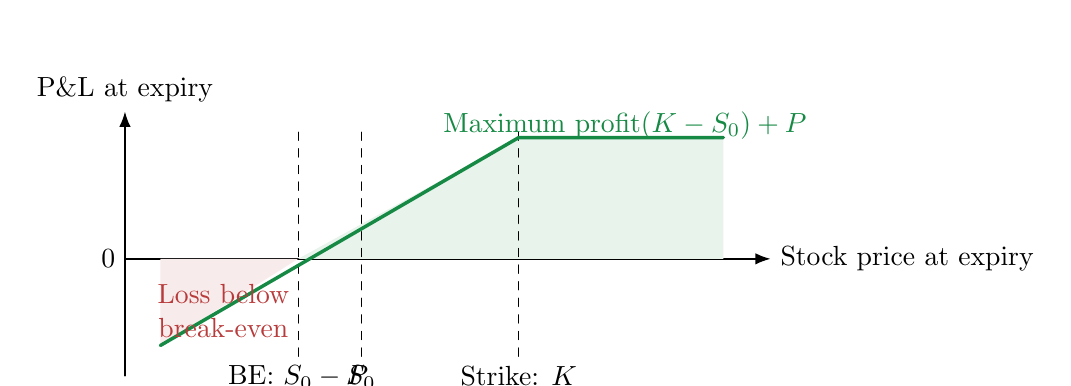
\begin{tikzpicture}[x=1cm,y=0.55cm,>=Latex,line cap=round]
    \draw[->,line width=0.55pt] (0,0) -- (8.2,0) node[right] {Stock price at expiry};
    \draw[->,line width=0.55pt] (0,-2.7) -- (0,3.4) node[above] {P\&L at expiry};
    \node[left] at (0,0) {0};
    \fill[bearc!10] (0.45,0) -- (0.45,-2) -- (2.2,0) -- cycle;
    \fill[bullc!10] (2.2,0) -- (5,2.8) -- (7.6,2.8) -- (7.6,0) -- cycle;
    \draw[dashed] (2.2,-2.25) -- (2.2,2.95);
    \draw[dashed] (3.0,-2.25) -- (3.0,2.95);
    \draw[dashed] (5.0,-2.25) -- (5.0,2.95);
    \draw[bullc,line width=1.25pt] (0.45,-2) -- (5,2.8) -- (7.6,2.8);
    \node[below,align=center] at (2.2,-2.25) {BE: \(S_0-P\)};
    \node[below,align=center] at (3.0,-2.25) {$S_0$};
    \node[below,align=center] at (5.0,-2.25) {Strike: \(K\)};
    \node[align=center,bullc] at (6.35,3.08) {Maximum profit\((K-S_0)+P\)};
    \node[align=center,bearc] at (1.25,-1.2) {Loss below\\break-even};
\end{tikzpicture}
\caption{Covered call payoff diagram.}
\end{figure}



\subsubsection{Key Levels and Formulas}

Let:
\begin{itemize}[leftmargin=*]
    \item \textbf{S₀} = Stock purchase price per share
    \item \textbf{K} = Strike price of the call sold
    \item \textbf{P} = Premium received per share
\end{itemize}

\begin{center}
\scriptsize
\setlength{\tabcolsep}{3pt}
\begin{tabular}{|L{4.42cm}|L{4.42cm}|L{4.42cm}|}
\hline
Metric & Formula & Intuition \\
\hline
\textbf{Maximum Profit} & (K − S₀) + P & Stock rises to K; you sell at K + you kept the premium \\
\hline
\textbf{Maximum Loss} & S₀ − P & Stock falls to zero; only the premium offsets the loss \\
\hline
\textbf{Break-even} & S₀ − P & The stock must fall below this before you have a net loss \\
\hline
\end{tabular}
\end{center}



\subsubsection{Worked Example (TSJ Stock)}

TSJ currently trades at \textbf{\$25.00}. You sell a 3-month call at strike \textbf{\$27} and collect \textbf{\$0.75/share} (\$75 per 100-share contract).

\textbf{Maximum Profit} = (\$27 − \$25) + \$0.75 = \textbf{\$2.75/share (\$275 per contract)}

\textbf{Break-even} = \$25 − \$0.75 = \textbf{\$24.25}

\textbf{Scenario 1 — Stock stays below \$27 at expiry:}
The call expires worthless. You keep all 100 shares plus the \$75 premium. Compared to just holding the stock alone, you have outperformed by \$75 for the period.

\textbf{Scenario 2 — Stock rises above \$27 at expiry:}
The call is exercised. You must sell your shares at \$27 regardless of how high the price is. If TSJ rises to \$35, you still only receive \$27. However, since you received \$0.75 premium, your effective sale price is \$27.75. \textbf{Only if the stock rises above \$27.75} would you have been better off not writing the call.



\subsubsection{Rolling Covered Calls}

When market conditions shift, a covered call position can be \textbf{"rolled"} — closing the current call and opening a new one with different terms — to tactically manage the position.

\textbf{Rolling Up:} Close the existing lower-strike call and open a new call at a higher strike. Used when the stock has risen significantly and the original call is deep in-the-money. By rolling up, you recapture some additional upside potential that was capped, while still collecting fresh premium.

\textbf{Rolling Down:} Close the existing call and open a new one at a lower strike price. A defensive move when the stock has fallen. The lower strike generates a higher premium relative to the current depressed stock price, partially compensating for the decline — but it lowers the upside cap further.

\textbf{Rolling Out:} Extend the expiry date by closing the near-term call and selling a new call with a later expiry date. Often done as the current call nears expiration and you want to maintain income generation. Rolling out can be combined with rolling up or rolling down to adjust both time and strike simultaneously.



\subsubsection{Advantages and Disadvantages}

\begin{center}
\scriptsize
\setlength{\tabcolsep}{3pt}
\begin{tabular}{|L{6.00cm}|L{6.00cm}|}
\hline
Pros & Cons \\
\hline
Generates reliable premium income from a held position & Caps all upside above the strike price \\
\hline
Reduces effective cost basis of the stock & Must be able to deliver 100 shares per contract if exercised \\
\hline
Provides partial downside protection equal to the premium & Does not meaningfully protect against a large price collapse \\
\hline
Suitable in IRA accounts (avoids triggering capital gains immediately) & If stock rallies far above the strike, the strategy significantly underperforms just holding shares \\
\hline
\end{tabular}
\end{center}



\subsubsection{When to Use / When to Avoid}

\begin{center}
\scriptsize
\setlength{\tabcolsep}{3pt}
\begin{tabular}{|L{6.00cm}|L{6.00cm}|}
\hline
Use When & Avoid When \\
\hline
Neutral to mildly bullish on the stock near-term & You expect a large price spike (you'd sacrifice the upside) \\
\hline
You're holding the stock long-term and want income & You are bearish (the premium only partially offsets a big decline) \\
\hline
You'd be comfortable selling the stock at the strike anyway & The stock faces high event risk (unexpected earnings, M\&A) \\
\hline
Implied volatility is elevated (premiums are rich) & You want full participation in a potential rally \\
\hline
\end{tabular}
\end{center}



\subsubsection{Related Strategies}

\textbf{Cash-Secured Put:} The mirror image of a covered call. Instead of owning the stock and selling a call, you sell a put while holding cash sufficient to buy the shares if assigned. Generates similar premium income, used when you're willing to acquire the stock at the put's strike price. (Covered in the previous chapter as "Short Put.")

\textbf{Collar Strategy:} Combines a covered call with a protective put. You own the stock, sell a call above the current price (generating income), and buy a put below it (providing downside protection). The call premium partially or fully offsets the cost of the put. The result: a defined range of outcomes — you cap upside at the call strike and cap downside at the put strike. More defensive than a plain covered call.

\begin{quote}
\emph{Collar formulas:}
\begin{itemize}[leftmargin=*]
    \item Maximum Gain = K\_call − S₀ + (Call Premium − Put Premium)
    \item Maximum Loss = S₀ − K\_put − (Call Premium − Put Premium)
\end{itemize}
\end{quote}

\textbf{Diagonal Spread:} Buy a longer-term call at one strike and sell a shorter-term call at a different (usually higher) strike. Benefits from time decay on the short leg and can be managed month-to-month as an ongoing income strategy with some directional flexibility.



\subsection{Protective Put (Married Put)}

\subsubsection{What It Is}

A \textbf{protective put} combines \textbf{owning shares of stock} with \textbf{buying a put option} on the same stock. The put option acts as insurance against a price decline — if the stock falls, the put gains in value, offsetting the losses. When the ratio of put options to shares is exactly 1:1 (one contract per 100 shares), the strategy is called a \textbf{married put}.

\textbf{Market Outlook:} Bullish on the stock long-term, but wanting a defined safety net against a near-term adverse event. The investor is unwilling to sell their shares (perhaps for tax reasons, long-term conviction, or restricted stock) but wants protection.



\subsubsection{Construction}

\begin{center}
\scriptsize
\setlength{\tabcolsep}{3pt}
\begin{tabular}{|L{6.00cm}|L{6.00cm}|}
\hline
Component & Action \\
\hline
Underlying Stock & \textbf{Own} (or simultaneously buy) 100 shares \\
\hline
Put Option & \textbf{Buy 1} put option at chosen strike K \\
\hline
\end{tabular}
\end{center}



\subsubsection{Intuition}

The protective put creates a \textbf{floor price} for your position. Think of it exactly like buying fire insurance on a house: you pay a premium every year (the put premium). If your house burns down (stock collapses), the insurance pays out (the put gains in value). If no fire occurs (stock rises), the premium is "wasted," but the peace of mind and capital protection were valuable.

The cost of protection is the premium paid, which permanently reduces net profit from the position — but without this cost, a large decline could cause irreversible capital damage.



\subsubsection{P\&L Diagram}

\begin{figure}[H]
\centering
\small
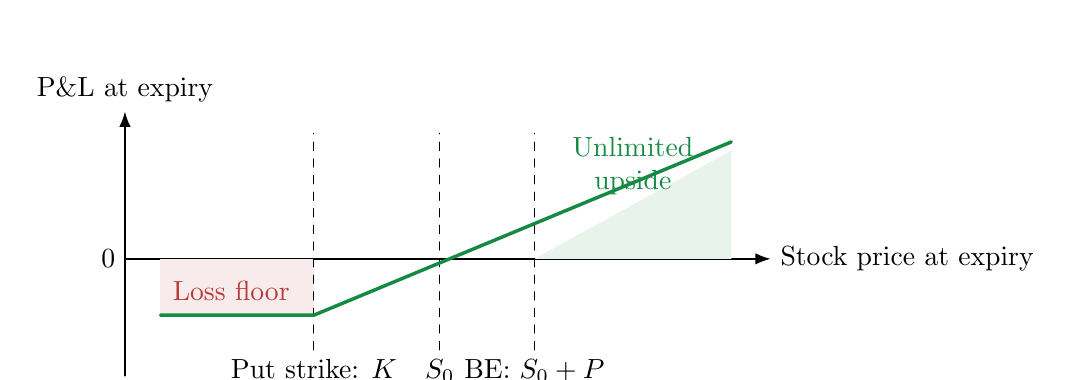
\begin{tikzpicture}[x=1cm,y=0.55cm,>=Latex,line cap=round]
    \draw[->,line width=0.55pt] (0,0) -- (8.2,0) node[right] {Stock price at expiry};
    \draw[->,line width=0.55pt] (0,-2.7) -- (0,3.4) node[above] {P\&L at expiry};
    \node[left] at (0,0) {0};
    \fill[bearc!10] (0.45,-1.3) -- (2.4,-1.3) -- (2.4,0) -- (0.45,0) -- cycle;
    \fill[bullc!10] (5.2,0) -- (7.7,2.5) -- (7.7,0) -- cycle;
    \draw[dashed] (2.4,-2.1) -- (2.4,2.9);
    \draw[dashed] (4.0,-2.1) -- (4.0,2.9);
    \draw[dashed] (5.2,-2.1) -- (5.2,2.9);
    \draw[bullc,line width=1.25pt] (0.45,-1.3) -- (2.4,-1.3) -- (7.7,2.7);
    \node[below,align=center] at (2.4,-2.1) {Put strike: \(K\)};
    \node[below,align=center] at (4.0,-2.1) {$S_0$};
    \node[below,align=center] at (5.2,-2.1) {BE: \(S_0+P\)};
    \node[align=center,bearc] at (1.35,-0.75) {Loss floor};
    \node[align=center,bullc] at (6.45,2.15) {Unlimited\\upside};
\end{tikzpicture}
\caption{Protective put payoff diagram.}
\end{figure}



\subsubsection{Key Levels and Formulas}

Let:
\begin{itemize}[leftmargin=*]
    \item \textbf{S₀} = Stock purchase price
    \item \textbf{K} = Put option strike price (the floor)
    \item \textbf{P} = Premium paid for the put
\end{itemize}

\begin{center}
\scriptsize
\setlength{\tabcolsep}{3pt}
\begin{tabular}{|L{4.42cm}|L{4.42cm}|L{4.42cm}|}
\hline
Metric & Formula & Intuition \\
\hline
\textbf{Maximum Loss} & (S₀ − K) + P & Unprotected gap from S₀ to K, plus the premium paid \\
\hline
\textbf{Maximum Profit} & Unlimited & Stock can rise infinitely; only the premium reduces the gain \\
\hline
\textbf{Break-even} & S₀ + P & Stock must rise by at least the premium paid to be net profitable \\
\hline
\end{tabular}
\end{center}



\subsubsection{Strike Price Choice: ATM vs. OTM Protective Puts}

The choice of strike determines how much protection you get versus how much you pay:

\textbf{At-the-Money (ATM) Protective Put} — strike K = S₀ (current stock price):
\begin{itemize}[leftmargin=*]
    \item Provides \textbf{100\% immediate protection} from the moment of purchase — any decline below S₀ is offset.
    \item Costs the most in premium (highest insurance cost).
    \item Typically used when buying the stock and the put simultaneously (classic married put).
\end{itemize}

\textbf{Out-of-the-Money (OTM) Protective Put} — strike K < S₀:
\begin{itemize}[leftmargin=*]
    \item Provides \textbf{partial protection} — the investor accepts losses between S₀ and K (the "deductible").
    \item Costs less (cheaper premium). The further OTM, the cheaper the put and the larger the accepted loss gap.
    \item Useful when the investor wants downside protection beyond a specific threshold.
\end{itemize}

\begin{quote}
\textbf{Example:} Investor owns stock at \$100, willing to accept up to a 5\% loss. They buy a put with strike \$95 (5\% OTM). If the stock falls to \$70, the put at \$95 limits total loss to roughly 5\% + premium paid, rather than 30\%.
\end{quote}



\subsubsection{Potential Outcomes}

\textbf{Stock rises:} The put expires worthless (or its value declines). You pay the premium as the cost of protection that was never needed. Net profit = price appreciation − premium paid. This is the "insurance premium" mentality — you don't regret paying for protection just because no disaster occurred.

\textbf{Stock falls below the strike:} The put is exercised (or sold for a gain). The put's gain offsets the stock's loss dollar-for-dollar below the strike. You have effectively locked in the strike price as your minimum exit value.

\textbf{Stock stays flat:} Small loss equal to the premium paid, as neither the stock appreciation nor the put payout compensates.



\subsubsection{Worked Example (GE Stock)}

\begin{itemize}[leftmargin=*]
    \item Investor bought \textbf{100 GE shares at \$10/share} (cost: \$1,000)
    \item GE has risen to \textbf{\$20/share} (unrealized gain: \$1,000)
    \item Investor is bullish but wants to protect the gains
    \item \textbf{Buys a put: Strike \$15, Premium \$0.75, Expiry 3 months}
\end{itemize}

Premium cost = \$0.75 × 100 = \textbf{\$75}

\textbf{Floor (worst-case scenario):}
If GE falls to \$10 or below, the put (strike \$15) generates a profit from \$15 down, offsetting losses. Net gain from \$10 baseline: (\$15 − \$10) − \$0.75 premium = \textbf{\$4.25/share (\$425 total) guaranteed minimum profit} above original purchase.

\textbf{Without the protective put:} If GE fell back to \$10, the investor's profit is \$0.

\textbf{Upside scenario (stock rises to \$30):}
\begin{itemize}[leftmargin=*]
    \item Put expires worthless (cost: \$75)
    \item Stock gain: (\$30 − \$10) × 100 = \$2,000
    \item Net: \$2,000 − \$75 = \textbf{\$1,925 net profit}
\end{itemize}

Without the put, the profit would be \$2,000. The \$75 was the cost of insurance.

\textbf{Interpretation:} The \$75 premium is the cost of peace of mind and capital protection. It guarantees a minimum profit of \$425 regardless of how low GE falls, while preserving full participation in any further upside.



\subsubsection{Pros and Cons}

\begin{center}
\scriptsize
\setlength{\tabcolsep}{3pt}
\begin{tabular}{|L{6.00cm}|L{6.00cm}|}
\hline
Pros & Cons \\
\hline
Preserves unlimited upside potential & Premium paid permanently reduces net returns \\
\hline
Creates a hard floor — losses cannot exceed the defined maximum & If the stock rises, the premium was an additional cost \\
\hline
Allows continued stock ownership during uncertainty & Must be renewed periodically (put options expire) \\
\hline
Works especially well when falling markets increase put values & OTM puts leave a gap of unprotected loss between S₀ and K \\
\hline
\end{tabular}
\end{center}



\subsection{Long Straddle}

\subsubsection{What It Is}

A \textbf{long straddle} involves simultaneously \textbf{buying one call and one put} on the same underlying asset, with \textbf{the same strike price (ATM) and the same expiry date}. You pay a net debit (premium for both options). The strategy profits from a \textbf{large price move in either direction} — you don't need to know which way the stock will go, only that it will move significantly.

\textbf{Market Outlook:} Highly uncertain direction but strong conviction that a large move is coming. Typically deployed before earnings releases, regulatory decisions, elections, or any major binary event.



\subsubsection{Construction}

\begin{center}
\scriptsize
\setlength{\tabcolsep}{3pt}
\begin{tabular}{|L{4.42cm}|L{4.42cm}|L{4.42cm}|}
\hline
Position & Action & Cost \\
\hline
ATM Call & \textbf{Buy 1} & Debit (call premium C) \\
\hline
ATM Put & \textbf{Buy 1} & Debit (put premium P\_p) \\
\hline
\textbf{Net} & Long Straddle & \textbf{Net Debit = C + P\_p} \\
\hline
\end{tabular}
\end{center}



\subsubsection{Intuition}

You are paying to own the right to profit from volatility in either direction. Think of it as placing two simultaneous directional bets — one up, one down — and needing only one to succeed by enough to cover the cost of both. The danger: if the stock barely moves (or the anticipated event produces no reaction), both options decay toward zero and the entire premium is lost.

The key driver of P\&L is not the direction of the move, but the \textbf{magnitude}. If you've paid \$10 in total premium, the stock must move more than \$10 from the strike for either option to generate net profit.



\subsubsection{P\&L Diagram}

The long straddle produces a distinctive \textbf{V-shape} (the inverse of the short straddle's pyramid):

\begin{figure}[H]
\centering
\small
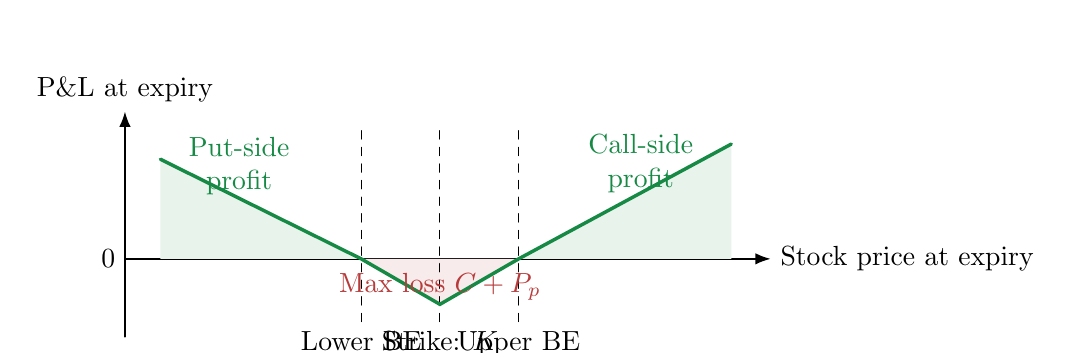
\begin{tikzpicture}[x=1cm,y=0.55cm,>=Latex,line cap=round]
    \draw[->,line width=0.55pt] (0,0) -- (8.2,0) node[right] {Stock price at expiry};
    \draw[->,line width=0.55pt] (0,-1.8) -- (0,3.4) node[above] {P\&L at expiry};
    \node[left] at (0,0) {0};
    \fill[bullc!10] (0.45,2.3) -- (3,0) -- (0.45,0) -- cycle;
    \fill[bearc!10] (3,0) -- (4,-1.05) -- (5,0) -- cycle;
    \fill[bullc!10] (5,0) -- (7.7,2.65) -- (7.7,0) -- cycle;
    \draw[dashed] (3,-1.45) -- (3,3.0);
    \draw[dashed] (4,-1.45) -- (4,3.0);
    \draw[dashed] (5,-1.45) -- (5,3.0);
    \draw[bullc,line width=1.25pt] (0.45,2.3) -- (3,0) -- (4,-1.05) -- (5,0) -- (7.7,2.65);
    \node[below,align=center] at (3,-1.45) {Lower BE};
    \node[below,align=center] at (4,-1.45) {Strike: \(K\)};
    \node[below,align=center] at (5,-1.45) {Upper BE};
    \node[align=center,bearc] at (4,-0.65) {Max loss \(C+P_p\)};
    \node[align=center,bullc] at (1.45,2.15) {Put-side\\profit};
    \node[align=center,bullc] at (6.55,2.2) {Call-side\\profit};
\end{tikzpicture}
\caption{Long straddle payoff diagram.}
\end{figure}

\begin{itemize}[leftmargin=*]
    \item \textbf{Left of BE₁:} Put is deep in-the-money. Strategy is profitable.
    \item \textbf{Between BE₁ and BE₂:} Both options partially or fully worthless. Net loss up to the total premium.
    \item \textbf{Right of BE₂:} Call is deep in-the-money. Strategy is profitable.
\end{itemize}



\subsubsection{Key Levels and Formulas}

Let:
\begin{itemize}[leftmargin=*]
    \item \textbf{K} = Strike price (same for both call and put)
    \item \textbf{C} = Call premium paid
    \item \textbf{P\_p} = Put premium paid
    \item \textbf{Total Premium} = C + P\_p
\end{itemize}

\begin{center}
\scriptsize
\setlength{\tabcolsep}{3pt}
\begin{tabular}{|L{6.00cm}|L{6.00cm}|}
\hline
Metric & Formula \\
\hline
\textbf{Maximum Loss} & C + P\_p (total premium paid) \\
\hline
\textbf{Maximum Profit (upside)} & Unlimited (stock → ∞) \\
\hline
\textbf{Maximum Profit (downside)} & K − Total Premium (if stock → 0) \\
\hline
\textbf{Upper Break-even (BE₂)} & K + Total Premium \\
\hline
\textbf{Lower Break-even (BE₁)} & K − Total Premium \\
\hline
\end{tabular}
\end{center}

\textbf{Profit when stock rises:} = Stock Price − K − Total Premium

\textbf{Profit when stock falls:} = K − Stock Price − Total Premium



\subsubsection{Risk to Be Aware Of}

The options market knows about upcoming events. When a significant event is anticipated, \textbf{implied volatility (IV) is already elevated} for those options, making the straddle more expensive. Option sellers price in the expected event. This means the straddle must profit from a move \emph{larger than what the market already expects} — simply having a large move is not enough if the market already priced in that large move through expensive premiums.



\subsubsection{Worked Example}

XYZ stock trades at \$50. Trader buys a straddle at the 100 strike:
\begin{itemize}[leftmargin=*]
    \item Call premium: \$22
    \item Put premium: \$20
    \item \textbf{Total Cost: \$42} (maximum loss)
\end{itemize}

On expiry, XYZ trades at \textbf{\$150}:
\begin{itemize}[leftmargin=*]
    \item The put expires worthless (stock above \$100 strike)
    \item Call payoff = \$150 − \$100 = \textbf{\$50 in-the-money}
    \item Net Profit = \$50 − \$42 = \textbf{\$8}
\end{itemize}

Upper break-even = \$100 + \$42 = \textbf{\$142}
Lower break-even = \$100 − \$42 = \textbf{\$58}

Simplified ATM example: Stock at \$120, straddle costs \$20 total (strike = \$120):
\begin{itemize}[leftmargin=*]
    \item Upper BE = \$120 + \$20 = \textbf{\$140}; Lower BE = \$120 − \$20 = \textbf{\$100}
    \item If stock rises to \$150 → Profit = (\$150 − \$120) − \$20 = \textbf{\$10}
    \item If stock falls to \$90 → Profit = (\$120 − \$90) − \$20 = \textbf{\$10}
    \item If stock stays at \$120 → \textbf{Loss = \$20} (maximum loss)
\end{itemize}



\subsection{Short Straddle}

\subsubsection{What It Is}

The exact inverse of the long straddle. You \textbf{sell one ATM call and one ATM put}, both at the same strike and expiry. You collect a net credit upfront and profit if the stock remains close to the strike through expiry.

\textbf{Market Outlook:} Very low volatility expected — the stock is range-bound and likely to expire near the strike.



\subsubsection{Construction}

\begin{center}
\scriptsize
\setlength{\tabcolsep}{3pt}
\begin{tabular}{|L{6.00cm}|L{6.00cm}|}
\hline
Position & Action \\
\hline
ATM Call & \textbf{Sell 1} \\
\hline
ATM Put & \textbf{Sell 1} \\
\hline
\textbf{Net} & Net Credit = C + P\_p \\
\hline
\end{tabular}
\end{center}



\subsubsection{P\&L Diagram}

The short straddle produces an \textbf{inverted V-shape (pyramid)}:

\begin{figure}[H]
\centering
\small
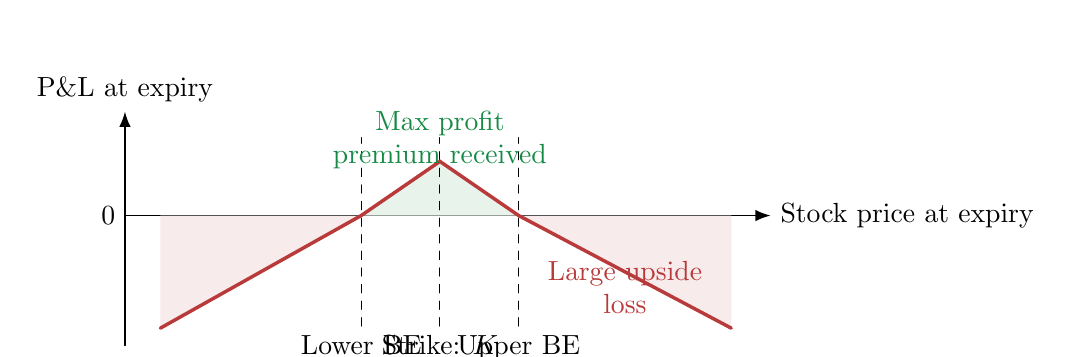
\begin{tikzpicture}[x=1cm,y=0.55cm,>=Latex,line cap=round]
    \draw[->,line width=0.55pt] (0,0) -- (8.2,0) node[right] {Stock price at expiry};
    \draw[->,line width=0.55pt] (0,-3.0) -- (0,2.4) node[above] {P\&L at expiry};
    \node[left] at (0,0) {0};
    \fill[bullc!10] (3,0) -- (4,1.25) -- (5,0) -- cycle;
    \fill[bearc!10] (0.45,-2.6) -- (3,0) -- (0.45,0) -- cycle;
    \fill[bearc!10] (5,0) -- (7.7,-2.6) -- (7.7,0) -- cycle;
    \draw[dashed] (3,-2.55) -- (3,1.8);
    \draw[dashed] (4,-2.55) -- (4,1.8);
    \draw[dashed] (5,-2.55) -- (5,1.8);
    \draw[bearc,line width=1.25pt] (0.45,-2.6) -- (3,0) -- (4,1.25) -- (5,0) -- (7.7,-2.6);
    \node[below,align=center] at (3,-2.55) {Lower BE};
    \node[below,align=center] at (4,-2.55) {Strike: \(K\)};
    \node[below,align=center] at (5,-2.55) {Upper BE};
    \node[align=center,bullc] at (4,1.75) {Max profit\\premium received};
    \node[align=center,bearc] at (6.35,-1.65) {Large upside\\loss};
\end{tikzpicture}
\caption{Short straddle payoff diagram.}
\end{figure}



\subsubsection{Key Levels}

\begin{center}
\scriptsize
\setlength{\tabcolsep}{3pt}
\begin{tabular}{|L{6.00cm}|L{6.00cm}|}
\hline
Metric & Formula \\
\hline
\textbf{Maximum Profit} & Total Premium Received (C + P\_p) \\
\hline
\textbf{Maximum Loss} & Unlimited (upside) / Stock → 0 (downside) \\
\hline
\textbf{Upper Break-even} & K + Total Premium \\
\hline
\textbf{Lower Break-even} & K − Total Premium \\
\hline
\end{tabular}
\end{center}



\subsubsection{Long Straddle vs. Short Straddle: Full Comparison}

\begin{center}
\scriptsize
\setlength{\tabcolsep}{3pt}
\begin{tabular}{|L{4.42cm}|L{4.42cm}|L{4.42cm}|}
\hline
Feature & Long Straddle & Short Straddle \\
\hline
\textbf{Entry} & Buy ATM call + Buy ATM put & Sell ATM call + Sell ATM put \\
\hline
\textbf{Net Cash Flow} & Net Debit (pay) & Net Credit (receive) \\
\hline
\textbf{Risk} & Limited (total premium paid) & Unlimited \\
\hline
\textbf{Reward} & Unlimited upside; large downside & Limited to premium received \\
\hline
\textbf{Bet on} & Large price move in any direction & Price stays near the strike \\
\hline
\textbf{Hurt by} & Lack of movement (time decay) & Large moves in either direction \\
\hline
\textbf{Helped by} & Rising implied volatility & Falling implied volatility \\
\hline
\textbf{P\&L Shape} & V-shape & Inverted V (pyramid) \\
\hline
\end{tabular}
\end{center}



\subsection{Long Strangle}

\subsubsection{What It Is}

A \textbf{long strangle} involves \textbf{buying an OTM call and an OTM put} on the same underlying asset, with \textbf{the same expiry but different strike prices} — the call strike is above the current price and the put strike is below it. Like the long straddle, it profits from a large move in either direction; unlike the straddle, it is \textbf{cheaper} (OTM options cost less) but requires a \textbf{larger move} to become profitable.

\textbf{Market Outlook:} Expects significant volatility but is uncertain of direction. Cheaper to set up than a straddle, making it attractive when ATM premiums are expensive.



\subsubsection{Construction}

\begin{center}
\scriptsize
\setlength{\tabcolsep}{3pt}
\begin{tabular}{|L{4.42cm}|L{4.42cm}|L{4.42cm}|}
\hline
Position & Action & Strike \\
\hline
OTM Call & \textbf{Buy 1} & K\_call > Current Price \\
\hline
OTM Put & \textbf{Buy 1} & K\_put < Current Price \\
\hline
\textbf{Net} & Net Debit & K\_put < Current Price < K\_call \\
\hline
\end{tabular}
\end{center}



\subsubsection{Intuition}

Think of the strangle as a straddle that has been "stretched outward." By purchasing options further from the money, you reduce the initial cost — but you create a wider dead zone between the two strikes where both options expire worthless. The stock must move even further than with a straddle before the trade becomes profitable. The trade-off: lower cost, larger required move, slightly better probability of profit on the short side.



\subsubsection{P\&L Diagram}

\begin{figure}[H]
\centering
\small
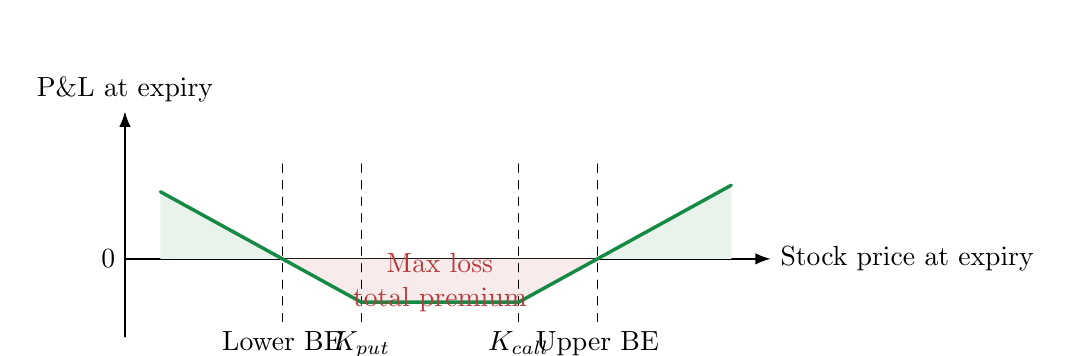
\begin{tikzpicture}[x=1cm,y=0.55cm,>=Latex,line cap=round]
    \draw[->,line width=0.55pt] (0,0) -- (8.2,0) node[right] {Stock price at expiry};
    \draw[->,line width=0.55pt] (0,-1.8) -- (0,3.4) node[above] {P\&L at expiry};
    \node[left] at (0,0) {0};
    \fill[bullc!10] (0.45,1.55) -- (2,0) -- (0.45,0) -- cycle;
    \fill[bearc!10] (2,0) -- (3,-1) -- (5,-1) -- (6,0) -- cycle;
    \fill[bullc!10] (6,0) -- (7.7,1.7) -- (7.7,0) -- cycle;
    \draw[dashed] (2,-1.45) -- (2,2.3);
    \draw[dashed] (3,-1.45) -- (3,2.3);
    \draw[dashed] (5,-1.45) -- (5,2.3);
    \draw[dashed] (6,-1.45) -- (6,2.3);
    \draw[bullc,line width=1.25pt] (0.45,1.55) -- (2,0) -- (3,-1) -- (5,-1) -- (6,0) -- (7.7,1.7);
    \node[below,align=center] at (2,-1.45) {Lower BE};
    \node[below,align=center] at (3,-1.45) {$K_{put}$};
    \node[below,align=center] at (5,-1.45) {$K_{call}$};
    \node[below,align=center] at (6,-1.45) {Upper BE};
    \node[align=center,bearc] at (4,-0.55) {Max loss\\total premium};
\end{tikzpicture}
\caption{Long strangle payoff diagram.}
\end{figure}



\subsubsection{Key Levels and Formulas}

Let:
\begin{itemize}[leftmargin=*]
    \item \textbf{K\_call} = Call strike (OTM, above current price)
    \item \textbf{K\_put} = Put strike (OTM, below current price)
    \item \textbf{C} = Call premium paid
    \item \textbf{P\_p} = Put premium paid
    \item \textbf{Total Premium} = C + P\_p
\end{itemize}

\begin{center}
\scriptsize
\setlength{\tabcolsep}{3pt}
\begin{tabular}{|L{6.00cm}|L{6.00cm}|}
\hline
Metric & Formula \\
\hline
\textbf{Maximum Loss} & Total Premium Paid (C + P\_p) \\
\hline
\textbf{Upper Break-even} & K\_call + Total Premium \\
\hline
\textbf{Lower Break-even} & K\_put − Total Premium \\
\hline
\textbf{Maximum Profit (upside)} & Unlimited \\
\hline
\textbf{Maximum Profit (downside)} & K\_put − Total Premium (if stock → 0) \\
\hline
\end{tabular}
\end{center}



\subsubsection{Worked Examples}

\textbf{Example 1 (Dave, March 2022):}
\begin{itemize}[leftmargin=*]
    \item Bought \$120 Put + \$130 Call
    \item Total premium = \textbf{\$10}
    \item Lower BE = \$120 − \$10 = \textbf{\$110}
    \item Upper BE = \$130 + \$10 = \textbf{\$140}
    \item Profitable if stock moves below \$110 or above \$140.
\end{itemize}

\textbf{Example 2 (Dan, ABC stock at \$200):}
\begin{itemize}[leftmargin=*]
    \item Call: Strike \$205, Premium \$5/share → \$500 total
    \item Put: Strike \$195, Premium \$3/share → \$300 total
    \item \textbf{Total Cost: \$800}
\end{itemize}

If stock falls to \$180 at expiry:
\begin{itemize}[leftmargin=*]
    \item Call expires worthless (lose \$500 premium)
    \item Put payoff: (\$195 − \$180) × 100 = \$1,500 gross; net put profit = \$1,500 − \$300 = \textbf{\$1,200}
    \item \textbf{Overall Profit = \$1,200 − \$500 = \$700}
\end{itemize}

If stock stays between \$195 and \$205:
\begin{itemize}[leftmargin=*]
    \item Both options expire OTM → \textbf{Maximum Loss = \$800}
\end{itemize}

Lower BE = \$195 − \$8 = \textbf{\$187}
Upper BE = \$205 + \$8 = \textbf{\$213}



\subsection{Short Strangle}

\subsubsection{What It Is}

A \textbf{short strangle} involves \textbf{selling an OTM call and an OTM put} on the same underlying, same expiry, but different strikes. You collect premium upfront and profit if the stock stays within a wide range. Compared to the short straddle, the profit zone is wider (less likely to breach a short strike) but the premium collected is lower (OTM options are cheaper).

\textbf{Market Outlook:} Range-bound, low-to-moderate volatility. You believe the stock will stay between the two short strikes.



\subsubsection{Construction}

\begin{center}
\scriptsize
\setlength{\tabcolsep}{3pt}
\begin{tabular}{|L{4.42cm}|L{4.42cm}|L{4.42cm}|}
\hline
Position & Action & Strike \\
\hline
OTM Call & \textbf{Sell 1} & K\_call above current price \\
\hline
OTM Put & \textbf{Sell 1} & K\_put below current price \\
\hline
\textbf{Net} & Net Credit & Premium collected \\
\hline
\end{tabular}
\end{center}



\subsubsection{P\&L Diagram}

\begin{figure}[H]
\centering
\small
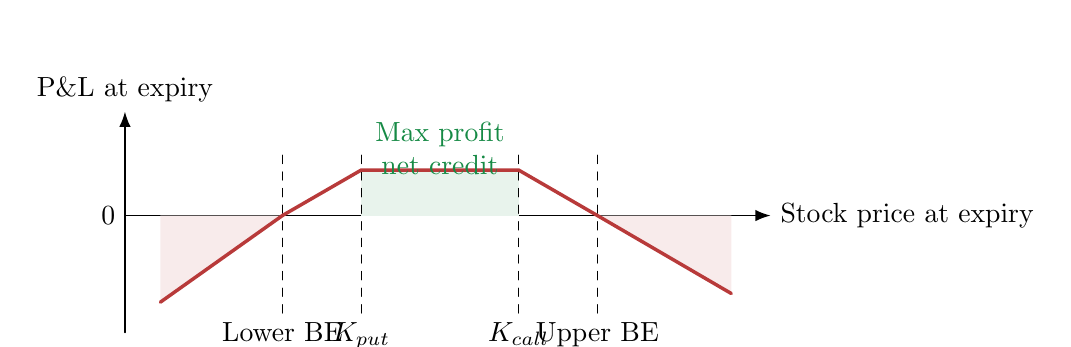
\begin{tikzpicture}[x=1cm,y=0.55cm,>=Latex,line cap=round]
    \draw[->,line width=0.55pt] (0,0) -- (8.2,0) node[right] {Stock price at expiry};
    \draw[->,line width=0.55pt] (0,-2.7) -- (0,2.4) node[above] {P\&L at expiry};
    \node[left] at (0,0) {0};
    \fill[bullc!10] (3,0) -- (3,1.05) -- (5,1.05) -- (5,0) -- cycle;
    \fill[bearc!10] (0.45,-2) -- (2,0) -- (0.45,0) -- cycle;
    \fill[bearc!10] (6,0) -- (7.7,-1.8) -- (7.7,0) -- cycle;
    \draw[dashed] (2,-2.25) -- (2,1.55);
    \draw[dashed] (3,-2.25) -- (3,1.55);
    \draw[dashed] (5,-2.25) -- (5,1.55);
    \draw[dashed] (6,-2.25) -- (6,1.55);
    \draw[bearc,line width=1.25pt] (0.45,-2) -- (2,0) -- (3,1.05) -- (5,1.05) -- (6,0) -- (7.7,-1.8);
    \node[below,align=center] at (2,-2.25) {Lower BE};
    \node[below,align=center] at (3,-2.25) {$K_{put}$};
    \node[below,align=center] at (5,-2.25) {$K_{call}$};
    \node[below,align=center] at (6,-2.25) {Upper BE};
    \node[align=center,bullc] at (4,1.55) {Max profit\\net credit};
\end{tikzpicture}
\caption{Short strangle payoff diagram.}
\end{figure}

\subsubsection{Key Levels}

\begin{center}
\scriptsize
\setlength{\tabcolsep}{3pt}
\begin{tabular}{|L{6.00cm}|L{6.00cm}|}
\hline
Metric & Formula \\
\hline
\textbf{Maximum Profit} & Net Premium Received (C + P\_p) \\
\hline
\textbf{Maximum Loss} & Unlimited (upside); large (downside) \\
\hline
\textbf{Upper Break-even} & K\_call + Net Premium \\
\hline
\textbf{Lower Break-even} & K\_put − Net Premium \\
\hline
\end{tabular}
\end{center}



\subsubsection{Short Straddle vs. Short Strangle}

\begin{center}
\scriptsize
\setlength{\tabcolsep}{3pt}
\begin{tabular}{|L{4.42cm}|L{4.42cm}|L{4.42cm}|}
\hline
Feature & Short Straddle & Short Strangle \\
\hline
\textbf{Strikes} & Both ATM (same strike) & Call OTM, Put OTM (different strikes) \\
\hline
\textbf{Premium Collected} & Higher (ATM options most expensive) & Lower (OTM options cheaper) \\
\hline
\textbf{Profit Zone} & Narrower — loss starts closer to strike & Wider — loss starts further from current price \\
\hline
\textbf{Risk of Breach} & Higher (any small move reduces profit) & Lower (stock must move further to cause a loss) \\
\hline
\textbf{Best For} & High IV environments where premium is rich & Normal-to-low IV environments; higher probability \\
\hline
\end{tabular}
\end{center}



\subsection{Straddle vs. Strangle: Choosing the Right Strategy}

\subsubsection{Premium and Probability Trade-off}

\begin{center}
\scriptsize
\setlength{\tabcolsep}{3pt}
\begin{tabular}{|L{4.42cm}|L{4.42cm}|L{4.42cm}|}
\hline
Factor & Straddle (ATM) & Strangle (OTM) \\
\hline
Premium paid (long) & Higher & Lower \\
\hline
Premium received (short) & Higher & Lower \\
\hline
Break-even distance & Narrower (smaller required move) & Wider (larger required move) \\
\hline
Probability of profit (short version) & Lower & Higher \\
\hline
Required move (long version) & Smaller & Larger \\
\hline
\end{tabular}
\end{center}

\subsubsection{The IVR (Implied Volatility Rank) Framework}

\textbf{Implied Volatility Rank (IVR)} measures where current IV sits relative to its 52-week range. IVR of 0\% means IV is at the annual low; IVR of 100\% means IV is at the annual high.

\textbf{When IVR is LOW → Prefer the SHORT STRANGLE}

In a low-IV environment, ATM options are relatively cheap — selling a straddle would not collect enough premium to justify the near-the-money risk. Going OTM with a strangle maximises the probability of success (wider profit range) while accepting the lower premium as appropriate for the subdued volatility environment. The focus is on \textbf{probability over premium}.

\textbf{When IVR is HIGH → Prefer the SHORT STRADDLE}

In a high-IV environment, ATM options are expensive — premiums are generous. Selling the straddle collects maximum premium at the peak of volatility. When IV subsequently contracts (as it typically does after a major event), the straddle's value collapses rapidly, allowing the seller to capture the profit much faster than usual. The aggressive ATM positioning is justified because the premium is large enough to provide wide enough break-even points. The focus is on \textbf{premium harvesting at IV peaks}.



\subsubsection{Converting to Defined-Risk Positions}

Accounts without margin approval (e.g., IRAs, basic brokerage accounts) cannot sell naked options. The solution is to \textbf{add wings} — buy additional far OTM options that cap the maximum loss:

\textbf{Short Straddle → Iron Butterfly}

Take the short straddle (sell ATM call + sell ATM put) and add wings:
\begin{itemize}[leftmargin=*]
    \item Buy a far OTM call above the short call strike (upper wing)
    \item Buy a far OTM put below the short put strike (lower wing)
\end{itemize}

The result is an \textbf{iron butterfly} — the same peaked profit shape but with a hard cap on maximum loss at the wing strikes. You sacrifice some premium for the wings, but your risk is fully defined.

\textbf{Short Strangle → Iron Condor}

Take the short strangle (sell OTM call + sell OTM put) and add wings:
\begin{itemize}[leftmargin=*]
    \item Buy a far OTM call above the short call (upper wing)
    \item Buy a far OTM put below the short put (lower wing)
\end{itemize}

The result is an \textbf{iron condor} — the same wide profit zone but with defined maximum losses at the wing strikes. In both cases, adding wings reduces the net premium collected but makes the position permissible in risk-defined accounts and removes unlimited risk.



\subsection{Butterfly Spread}

\subsubsection{What It Is}

A \textbf{butterfly spread} is a \textbf{neutral, range-bound, limited risk and limited profit strategy} that targets a specific stock price at expiry. It uses \textbf{three strike prices} (K₁ lower, K₂ middle, K₃ upper) and \textbf{four option contracts}. The outer strikes (K₁ and K₃) must be equidistant from the middle strike (K₂ − K₁ = K₃ − K₂).

\textbf{Market Outlook:} Neutral — the investor expects the stock to remain very close to the middle strike K₂ at expiry, with minimal price movement.

The name comes from the shape of the P\&L diagram: the two outer wings (buy positions) and the middle body (sold positions) resemble a butterfly when plotted.



\subsubsection{General Structure}

\begin{center}
\small
\begin{tabular}{|L{3cm}|L{3cm}|L{3cm}|L{4.5cm}|}
\hline
\textbf{Action} & \textbf{Quantity} & \textbf{Strike} & \textbf{Role} \\
\hline
Buy & 1 option & $K_1$ & Left wing \\
\hline
Sell & 2 options & $K_2$ & Body; maximum profit point \\
\hline
Buy & 1 option & $K_3$ & Right wing \\
\hline
\end{tabular}
\end{center}
where $K_1 < K_2 < K_3$ and $(K_2 - K_1) = (K_3 - K_2)$.



\subsubsection{P\&L Diagram (Long Call Butterfly — the template shape)}

\begin{figure}[H]
\centering
\small
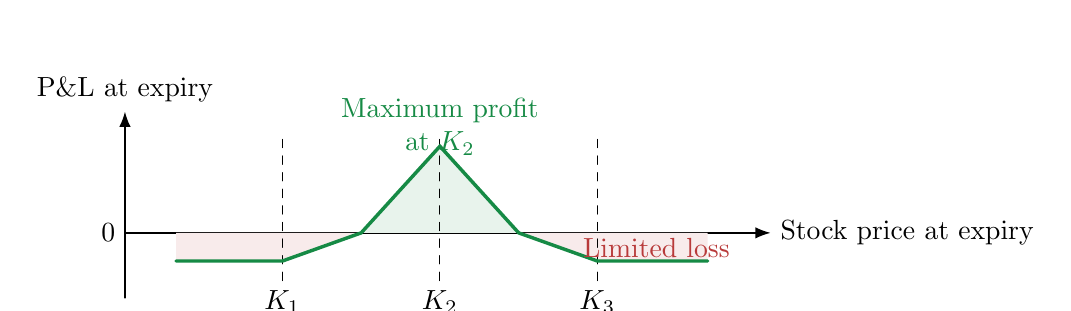
\begin{tikzpicture}[x=1cm,y=0.55cm,>=Latex,line cap=round]
    \draw[->,line width=0.55pt] (0,0) -- (8.2,0) node[right] {Stock price at expiry};
    \draw[->,line width=0.55pt] (0,-1.5) -- (0,2.8) node[above] {P\&L at expiry};
    \node[left] at (0,0) {0};
    \fill[bullc!10] (3,0) -- (4,2) -- (5,0) -- cycle;
    \fill[bearc!10] (0.65,-0.65) -- (2,-0.65) -- (3,0) -- (0.65,0) -- cycle;
    \fill[bearc!10] (5,0) -- (6,-0.65) -- (7.4,-0.65) -- (7.4,0) -- cycle;
    \draw[dashed] (2,-1.1) -- (2,2.35);
    \draw[dashed] (4,-1.1) -- (4,2.35);
    \draw[dashed] (6,-1.1) -- (6,2.35);
    \draw[bullc,line width=1.25pt] (0.65,-0.65) -- (2,-0.65) -- (3,0) -- (4,2) -- (5,0) -- (6,-0.65) -- (7.4,-0.65);
    \node[below,align=center] at (2,-1.1) {$K_1$};
    \node[below,align=center] at (4,-1.1) {$K_2$};
    \node[below,align=center] at (6,-1.1) {$K_3$};
    \node[align=center,bullc] at (4,2.45) {Maximum profit\\at $K_2$};
    \node[align=center,bearc] at (6.75,-0.35) {Limited loss};
\end{tikzpicture}
\caption{Long butterfly payoff diagram.}
\end{figure}



\subsubsection{Long Call Butterfly}

\textbf{Construction:}
\begin{itemize}[leftmargin=*]
    \item \textbf{Buy} 1 call at K₁ (lower strike)
    \item \textbf{Sell} 2 calls at K₂ (middle strike)
    \item \textbf{Buy} 1 call at K₃ (upper strike)
\end{itemize}

\textbf{Net:} Net Debit (you pay to enter)

\textbf{When to use:} When you believe the stock price will remain very close to K₂ at expiry — low volatility expectation.

\begin{center}
\scriptsize
\setlength{\tabcolsep}{3pt}
\begin{tabular}{|L{6.00cm}|L{6.00cm}|}
\hline
Metric & Formula \\
\hline
\textbf{Maximum Profit} & (K₂ − K₁) − Net Premium Paid \\
\hline
\textbf{Maximum Loss} & Net Premium Paid \\
\hline
\textbf{Lower BE} & K₁ + Net Premium Paid \\
\hline
\textbf{Upper BE} & K₃ − Net Premium Paid \\
\hline
\end{tabular}
\end{center}

Maximum profit is achieved when the stock closes \textbf{exactly at K₂} at expiry (both short calls expire at-the-money, the lower long call is in-the-money by the spread width, the upper long call expires worthless).



\subsubsection{Short Call Butterfly}

\textbf{Construction:}
\begin{itemize}[leftmargin=*]
    \item \textbf{Sell} 1 call at K₁
    \item \textbf{Buy} 2 calls at K₂
    \item \textbf{Sell} 1 call at K₃
\end{itemize}

\textbf{Net:} Net Credit

\textbf{When to use:} When you expect a significant move in either direction (the opposite of the long call butterfly). Acts like a cheaper straddle with limited, defined risk.

\begin{center}
\scriptsize
\setlength{\tabcolsep}{3pt}
\begin{tabular}{|L{6.00cm}|L{6.00cm}|}
\hline
Metric & Formula \\
\hline
\textbf{Maximum Profit} & Net Credit Received \\
\hline
\textbf{Maximum Loss} & (K₂ − K₁) − Net Credit Received \\
\hline
\textbf{Profit occurs} & When stock ≤ K₁ or ≥ K₃ at expiry \\
\hline
\textbf{Max Loss occurs} & When stock closes exactly at K₂ \\
\hline
\end{tabular}
\end{center}



\subsubsection{Long Put Butterfly}

\textbf{Construction:}
\begin{itemize}[leftmargin=*]
    \item \textbf{Buy} 1 put at K₁
    \item \textbf{Sell} 2 puts at K₂
    \item \textbf{Buy} 1 put at K₃
\end{itemize}

Functionally equivalent in profit/loss profile to the long call butterfly (by put-call parity). Maximum profit when stock closes at K₂; maximum loss at or beyond the wing strikes.



\subsubsection{Short Put Butterfly}

\textbf{Construction:}
\begin{itemize}[leftmargin=*]
    \item \textbf{Sell} 1 put at K₁
    \item \textbf{Buy} 2 puts at K₂
    \item \textbf{Sell} 1 put at K₃
\end{itemize}

Equivalent to the short call butterfly — profits from a large move in either direction; maximum loss at K₂.



\subsubsection{Iron Butterfly}

\textbf{What it is:} The \textbf{iron butterfly} is the defined-risk version of a short straddle. Instead of using only calls or only puts, it mixes both: selling an ATM straddle and buying OTM wings to cap losses. It is what you get when you convert a short straddle into a defined-risk position.

\textbf{Construction:}

\begin{center}
\scriptsize
\setlength{\tabcolsep}{3pt}
\begin{tabular}{|L{3.31cm}|L{3.31cm}|L{3.31cm}|L{3.31cm}|}
\hline
Position & Action & Strike & Role \\
\hline
OTM Put & \textbf{Buy 1} & K₁ (below K₂) & Lower wing \\
\hline
ATM Put & \textbf{Sell 1} & K₂ & Body \\
\hline
ATM Call & \textbf{Sell 1} & K₂ & Body \\
\hline
OTM Call & \textbf{Buy 1} & K₃ (above K₂) & Upper wing \\
\hline
\end{tabular}
\end{center}

\textbf{Net:} Net Credit

\textbf{P\&L shape:} Identical to the long call butterfly — peaked at K₂, losses capped at the wing strikes. The iron butterfly has the same shape as the long call butterfly but is constructed differently (using a mix of puts and calls).

\begin{center}
\scriptsize
\setlength{\tabcolsep}{3pt}
\begin{tabular}{|L{6.00cm}|L{6.00cm}|}
\hline
Metric & Formula \\
\hline
\textbf{Maximum Profit} & Net Credit Received \\
\hline
\textbf{Maximum Loss} & (K₂ − K₁) − Net Credit \\
\hline
\textbf{Lower BE} & K₂ − Net Credit \\
\hline
\textbf{Upper BE} & K₂ + Net Credit \\
\hline
\end{tabular}
\end{center}

\textbf{Key Insight:} The iron butterfly produces the same economics as the short straddle, but with defined maximum loss — making it suitable for risk-defined and IRA accounts.



\subsubsection{Reverse Iron Butterfly}

\textbf{What it is:} The reverse (short) iron butterfly is the \textbf{defined-risk version of a long straddle}. Used when expecting a significant move in either direction but wanting to define the maximum loss.

\textbf{Construction:}

\begin{center}
\scriptsize
\setlength{\tabcolsep}{3pt}
\begin{tabular}{|L{4.42cm}|L{4.42cm}|L{4.42cm}|}
\hline
Position & Action & Strike \\
\hline
OTM Put & \textbf{Sell 1} & K₁ \\
\hline
ATM Put & \textbf{Buy 1} & K₂ \\
\hline
ATM Call & \textbf{Buy 1} & K₂ \\
\hline
OTM Call & \textbf{Sell 1} & K₃ \\
\hline
\end{tabular}
\end{center}

\textbf{Net:} Net Debit

\textbf{Maximum Loss:} Net Debit Paid (defined and limited — unlike the unlimited risk of a naked long call and long put at expiry in theory this is already limited, but this structure is about controlling risk with the outer short legs providing credits)

\textbf{Maximum Profit:} Achieved when stock closes below K₁ or above K₃ at expiry.



\subsubsection{Butterfly Strategy Summary}

\begin{center}
\scriptsize
\setlength{\tabcolsep}{3pt}
\begin{tabular}{|L{2.65cm}|L{2.65cm}|L{2.65cm}|L{2.65cm}|L{2.65cm}|}
\hline
Type & Net & Max Profit Condition & Max Loss Condition & Outlook \\
\hline
Long Call Butterfly & Debit & Stock at K₂ at expiry & Stock ≤ K₁ or ≥ K₃ & Neutral/low volatility \\
\hline
Short Call Butterfly & Credit & Stock ≤ K₁ or ≥ K₃ & Stock at K₂ & Expects large move \\
\hline
Long Put Butterfly & Debit & Stock at K₂ at expiry & Stock ≤ K₁ or ≥ K₃ & Neutral/low volatility \\
\hline
Short Put Butterfly & Credit & Stock ≤ K₁ or ≥ K₃ & Stock at K₂ & Expects large move \\
\hline
Iron Butterfly & Credit & Stock at K₂ at expiry & Stock ≤ K₁ or ≥ K₃ & Neutral; defined-risk short straddle \\
\hline
Reverse Iron Butterfly & Debit & Stock ≤ K₁ or ≥ K₃ & Stock at K₂ & Volatile; defined-risk long straddle \\
\hline
\end{tabular}
\end{center}



\subsubsection{Worked Example 1: Short Call Butterfly (XYZ at \$50)}

Investor expects price to move significantly from \$50. Sets up a short call butterfly:
\begin{itemize}[leftmargin=*]
    \item \textbf{Sell} 1 call at K₁ = \$45 → receive \$7 premium
    \item \textbf{Buy} 2 calls at K₂ = \$50 → pay \$7 total for both
    \item \textbf{Sell} 1 call at K₃ = \$55 → receive \$1 premium
\end{itemize}

\textbf{Net Credit} = \$7 + \$1 − \$7 = \textbf{\$1 per share}

\textbf{Maximum Profit} = Net Credit = \textbf{\$1} (if stock ≤ \$45 or ≥ \$55 at expiry)

\textbf{Maximum Loss} = (K₂ − K₁) − Net Credit = (\$50 − \$45) − \$1 = \textbf{\$4}
(Occurs if stock closes at \$50 at expiry)

This strategy gives defined risk (\$4 max loss) and a small credit (\$1 max gain) for a bet on movement.



\subsubsection{Worked Example 2: Long Call Butterfly (Apple at \$180)}

Stephens expects Apple to remain near \$180. Sets up a long call butterfly:
\begin{itemize}[leftmargin=*]
    \item \textbf{Buy} 1 call at K₁ = \$170 → pays \$5 premium
    \item \textbf{Sell} 2 calls at K₂ = \$180 → receives \$6 total (\$3 each)
    \item \textbf{Buy} 1 call at K₃ = \$190 → pays \$2 premium
\end{itemize}

\textbf{Net Cost (Debit)} = \$6 − \$5 − \$2 = \textbf{\$1 per share}

\textbf{Maximum Profit} = (K₂ − K₁) − Net Debit = (\$180 − \$170) − \$1 = \textbf{\$9}
(Occurs when Apple closes exactly at \$180 at expiry)

\textbf{Maximum Loss} = Net Debit = \textbf{\$1}
(Occurs when stock ≤ \$170 or ≥ \$190 at expiry)

\textbf{Break-even Points:}
\begin{itemize}[leftmargin=*]
    \item Lower BE = \$170 + \$1 = \textbf{\$171}
    \item Upper BE = \$190 − \$1 = \textbf{\$189}
\end{itemize}

This is the butterfly's elegant risk/reward in practice: \textbf{risk \$1 to potentially earn \$9} — a 9:1 reward-to-risk ratio — but only if the stock closes precisely at \$180.



\subsubsection{Butterfly vs. Straddle: Key Differences}

\begin{center}
\scriptsize
\setlength{\tabcolsep}{3pt}
\begin{tabular}{|L{4.42cm}|L{4.42cm}|L{4.42cm}|}
\hline
Feature & Long Call Butterfly & Long Straddle \\
\hline
\textbf{Strikes used} & 3 (K₁, K₂, K₃) & 1 (same for both options) \\
\hline
\textbf{Number of legs} & 4 & 2 \\
\hline
\textbf{Risk} & Limited to net debit & Limited to total premium \\
\hline
\textbf{Reward} & Limited (capped at K₂ profit) & Unlimited (upside) \\
\hline
\textbf{Profit when} & Stock is near K₂ (low volatility) & Stock makes a large move (high volatility) \\
\hline
\textbf{P\&L shape} & Peaked tent & V-shape \\
\hline
\textbf{Break-even} & Add/subtract premium from outer strikes & Add/subtract premium from the single middle strike \\
\hline
\end{tabular}
\end{center}



\subsection{Iron Condor}

\subsubsection{What It Is}

The \textbf{iron condor} is a \textbf{four-legged, fully defined-risk, neutral strategy} that profits from \textbf{low volatility and a range-bound market}. It is constructed by combining a \textbf{bull put spread} below the market price and a \textbf{bear call spread} above the market price, collecting a net credit and profiting when the underlying stays within the two short strikes at expiry.

The iron condor is essentially the defined-risk version of the \textbf{short strangle} — adding wings (long options at outer strikes) converts an unlimited-risk short strangle into a defined-risk iron condor.

\textbf{Market Outlook:} Neutral to mildly directional (can be tilted). Best suited for range-bound markets, index options, or ETFs with predictable, low-volatility behaviour.



\subsubsection{Construction}

\begin{center}
\scriptsize
\setlength{\tabcolsep}{3pt}
\begin{tabular}{|L{2.65cm}|L{2.65cm}|L{2.65cm}|L{2.65cm}|L{2.65cm}|}
\hline
Leg & Position & Action & Strike & Role \\
\hline
1 & Long Put & \textbf{Buy} & K₁ (lowest) & Lower wing (limits downside loss) \\
\hline
2 & Short Put & \textbf{Sell} & K₂ (lower middle) & Bull put spread — earns credit below market \\
\hline
3 & Short Call & \textbf{Sell} & K₃ (upper middle) & Bear call spread — earns credit above market \\
\hline
4 & Long Call & \textbf{Buy} & K₄ (highest) & Upper wing (limits upside loss) \\
\hline
\end{tabular}
\end{center}

\textbf{Strike ordering:} K₁ < K₂ < Current Price < K₃ < K₄

\textbf{Legs 1 \& 2} form the \textbf{Bull Put Spread} (net credit; profits if stock stays above K₂)
\textbf{Legs 3 \& 4} form the \textbf{Bear Call Spread} (net credit; profits if stock stays below K₃)

\textbf{Net Position:} Net Credit collected (the combined short premiums exceed the combined wing costs)



\subsubsection{Intuition}

The iron condor places a fence around the current stock price — a lower fence (the put spread) and an upper fence (the call spread). As long as the stock stays inside the fences at expiry, both spreads expire worthless and you keep the full premium. Time decay works in your favour every single day. The long wings (bought at K₁ and K₄) define the maximum possible loss and make the strategy permissible in risk-defined accounts.



\subsubsection{P\&L Diagram}

\begin{figure}[H]
\centering
\small
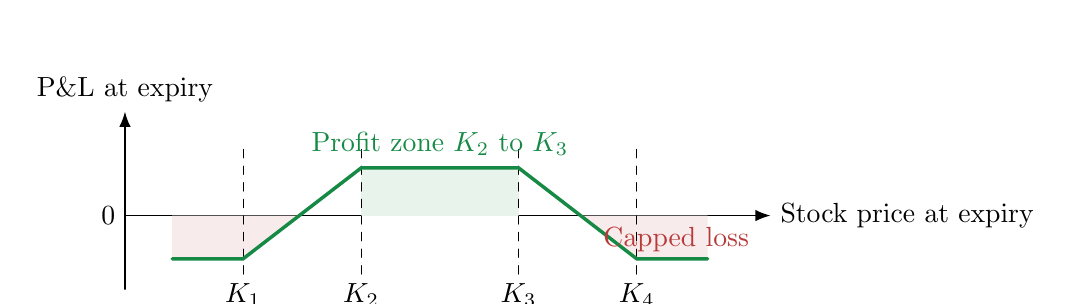
\begin{tikzpicture}[x=1cm,y=0.55cm,>=Latex,line cap=round]
    \draw[->,line width=0.55pt] (0,0) -- (8.2,0) node[right] {Stock price at expiry};
    \draw[->,line width=0.55pt] (0,-1.7) -- (0,2.4) node[above] {P\&L at expiry};
    \node[left] at (0,0) {0};
    \fill[bullc!10] (3,0) -- (3,1.1) -- (5,1.1) -- (5,0) -- cycle;
    \fill[bearc!10] (0.6,-1) -- (1.5,-1) -- (2.25,0) -- (0.6,0) -- cycle;
    \fill[bearc!10] (5.75,0) -- (6.5,-1) -- (7.4,-1) -- (7.4,0) -- cycle;
    \draw[dashed] (1.5,-1.35) -- (1.5,1.65);
    \draw[dashed] (3,-1.35) -- (3,1.65);
    \draw[dashed] (5,-1.35) -- (5,1.65);
    \draw[dashed] (6.5,-1.35) -- (6.5,1.65);
    \draw[bullc,line width=1.25pt] (0.6,-1) -- (1.5,-1) -- (3,1.1) -- (5,1.1) -- (6.5,-1) -- (7.4,-1);
    \node[below,align=center] at (1.5,-1.35) {$K_1$};
    \node[below,align=center] at (3,-1.35) {$K_2$};
    \node[below,align=center] at (5,-1.35) {$K_3$};
    \node[below,align=center] at (6.5,-1.35) {$K_4$};
    \node[align=center,bullc] at (4,1.65) {Profit zone \(K_2\) to \(K_3\)};
    \node[align=center,bearc] at (7.0,-0.55) {Capped loss};
\end{tikzpicture}
\caption{Iron condor payoff diagram.}
\end{figure}

\begin{itemize}[leftmargin=*]
    \item \textbf{Between K₂ and K₃ at expiry:} All four options expire OTM → Maximum Profit = Net Credit
    \item \textbf{Between K₁ and K₂ (or K₃ and K₄):} The closer short spread moves partially ITM → Partial loss
    \item \textbf{Below K₁ or Above K₄:} The closer spread is fully ITM → Maximum Loss
\end{itemize}



\subsubsection{Key Levels and Formulas}

Let:
\begin{itemize}[leftmargin=*]
    \item \textbf{Net Credit} = (K₂ premium + K₃ premium) − (K₁ premium + K₄ premium)
    \item \textbf{Spread Width} = K₂ − K₁ = K₄ − K₃ (common to use equal widths)
\end{itemize}

\begin{center}
\scriptsize
\setlength{\tabcolsep}{3pt}
\begin{tabular}{|L{6.00cm}|L{6.00cm}|}
\hline
Metric & Formula \\
\hline
\textbf{Maximum Profit} & Net Credit Received \\
\hline
\textbf{Maximum Loss} & Spread Width − Net Credit \\
\hline
\textbf{Lower Break-even (BE₁)} & K₂ − Net Credit \\
\hline
\textbf{Upper Break-even (BE₂)} & K₃ + Net Credit \\
\hline
\end{tabular}
\end{center}

\textbf{Note:} Maximum loss always exceeds maximum profit in an iron condor. This is by design — it is a \textbf{high-probability, lower-reward strategy}. You win more often than you lose, but when you do lose, the loss is larger than a single win.



\subsubsection{Step-by-Step Construction}

\textbf{Step 1 — Select the security:} Choose a stock, ETF, or index with \textbf{low expected volatility}. Prefer highly liquid underlyings with tight bid-ask spreads and deep open interest (e.g., Nifty 50 index, SPY, QQQ). Liquidity is critical for entering and exiting all four legs efficiently.

\textbf{Step 2 — Determine expiry:} Options with \textbf{30–60 days to expiry} are the most common for iron condors — they balance sufficient time-decay with manageable risk. Closer expirations (< 2 weeks) have faster theta but are more sensitive to sudden moves. Longer expirations (60+ days) have slower decay but greater exposure to volatility changes (vega risk).

\textbf{Step 3 — Select strike prices:} The short put (K₂) and short call (K₃) should have a \textbf{low probability of being breached at expiry} — typically a delta of 0.15 to 0.30, representing approximately 15–30\% probability of expiring ITM. The long wings (K₁ and K₄) are placed further OTM — typically the next available strike or a fixed number of points away — to define the maximum loss.

\textbf{Step 4 — Calculate net credit:} Net Credit = Premiums received (K₂ + K₃) − Premiums paid (K₁ + K₄). This is your maximum profit per contract. Multiply by lot size (e.g., × 100 shares) for total dollar value.

\textbf{Step 5 — Execute all four legs simultaneously:} Place as a single iron condor order. Avoid legging in individually — it creates unintended directional risk during the filling process.

\textbf{Step 6 — Manage the trade:} Watch for the stock approaching a short strike. If a short option is breached or close to being breached, consider closing the threatened spread, rolling it out or wider, or taking a defined partial loss rather than riding to maximum loss.



\subsubsection{Worked Example (VOO ETF at \$450)}

\textbf{Setup:} VOO ETF trades at \$450. Trader expects low volatility over 30 days. Sells an iron condor.

\begin{center}
\scriptsize
\setlength{\tabcolsep}{3pt}
\begin{tabular}{|L{3.31cm}|L{3.31cm}|L{3.31cm}|L{3.31cm}|}
\hline
Leg & Strike (\$) & Premium (\$) & Action \\
\hline
Long Put & 435 & −1.00 & Buy (debit) \\
\hline
Short Put & 440 & +2.00 & Sell (credit) \\
\hline
Short Call & 460 & +2.00 & Sell (credit) \\
\hline
Long Call & 465 & −1.00 & Buy (debit) \\
\hline
\end{tabular}
\end{center}

\textbf{Net Credit} = (\$2 + \$2) − (\$1 + \$1) = \textbf{\$2.00/share = \$200 per contract}

\textbf{Spread Width} = \$440 − \$435 = \$5 (each spread is \$5 wide)

\textbf{Maximum Profit} = \$200 per contract (stock stays between \$440 and \$460)

\textbf{Maximum Loss} = (\$5 − \$2) × 100 = \textbf{\$300 per contract} (stock below \$435 or above \$465)

\textbf{Break-even Points:}
\begin{itemize}[leftmargin=*]
    \item Lower BE = \$440 − \$2 = \textbf{\$438}
    \item Upper BE = \$460 + \$2 = \textbf{\$462}
\end{itemize}

\textbf{Risk-Reward Ratio} = \$200 / \$300 = 0.67 (risk \$3 to make \$2 — high probability compensates)

\textbf{Full P\&L Table:}

\begin{center}
\scriptsize
\setlength{\tabcolsep}{3pt}
\begin{tabular}{|L{4.42cm}|L{4.42cm}|L{4.42cm}|}
\hline
VOO Price at Expiry & Outcome & Profit/Loss \\
\hline
\$450 (inside range) & All options expire worthless & \textbf{+\$200} \\
\hline
\$445 (inside range) & All options expire worthless & \textbf{+\$200} \\
\hline
\$438 (lower break-even) & Short put partially ITM & \textbf{\$0} \\
\hline
\$462 (upper break-even) & Short call partially ITM & \textbf{\$0} \\
\hline
\$435 or below & Put spread fully ITM & \textbf{−\$300} \\
\hline
\$465 or above & Call spread fully ITM & \textbf{−\$300} \\
\hline
\end{tabular}
\end{center}

The trade is profitable as long as VOO stays between \$438 and \$462 — a ±5.3\% range from the current price of \$450. In a stable, low-volatility environment, this is a high-probability outcome.



\subsubsection{Adjusting the Iron Condor: Bullish and Bearish Bias}

The standard iron condor is symmetric. By adjusting where the spreads are placed, you can introduce a directional lean:

\textbf{Bullish Iron Condor:} Move K₂ (short put) \textbf{higher/closer} to the current price. The put spread is closer to the money, collecting more premium. Profits if the stock rises or stays flat; more vulnerable to a downward move.

\textbf{Bearish Iron Condor:} Move K₃ (short call) \textbf{lower/closer} to the current price. Profits if the stock falls or stays flat; more vulnerable to an upward move.

\begin{quote}
\textbf{Best practice:} Apply bullish adjustments in uptrends and bearish adjustments in downtrends. These tweaks maintain the time-decay and defined-risk structure while allowing the iron condor to align with a mild directional view.
\end{quote}



\subsubsection{Advantages and Disadvantages}

\begin{center}
\scriptsize
\setlength{\tabcolsep}{3pt}
\begin{tabular}{|L{6.00cm}|L{6.00cm}|}
\hline
Pros & Cons \\
\hline
\textbf{Defined risk} — maximum loss is fixed and known before entry & \textbf{Capped reward} — maximum profit is limited to the net credit \\
\hline
\textbf{High probability of profit} — wide profit zone appropriate for range-bound markets & \textbf{Assignment risk} — short options can be assigned early (though rare before expiry) \\
\hline
\textbf{Time decay is positive} — theta works in favour every day inside the profit range & \textbf{Volatility spike risk} — rising IV increases all option values, hurting the short spreads \\
\hline
\textbf{Capital efficient} — requires only margin for the spread width, not the full stock value & \textbf{4-leg commissions} reduce net profit, especially for small accounts \\
\hline
\textbf{Flexible} — can be adjusted (rolled, legged out of) as conditions change & \textbf{Active management required} if stock approaches a short strike \\
\hline
\textbf{Works in low-volatility markets} which are most common market conditions & Max profit/max loss ratio < 1 (you often make less than you risk per trade) \\
\hline
\end{tabular}
\end{center}



\subsection{Strategy Selector: Quick Reference}

\begin{center}
\scriptsize
\setlength{\tabcolsep}{3pt}
\begin{tabular}{|L{2.21cm}|L{2.21cm}|L{2.21cm}|L{2.21cm}|L{2.21cm}|L{2.21cm}|}
\hline
Strategy & Structure & Net Entry & Risk & Reward & Use When \\
\hline
\textbf{Covered Call} & Long stock + Short OTM call & Credit & Stock falls to zero (minus premium) & Limited (capped at strike) & Holding stock long-term; want income; neutral outlook \\
\hline
\textbf{Protective Put} & Long stock + Long put & Debit & Limited (premium paid + gap to strike) & Unlimited upside & Bullish but want downside hedge; protecting gains \\
\hline
\textbf{Collar} & Long stock + Short call + Long put & Low debit or zero & Limited (defined range) & Limited (defined range) & Want protection with minimal cost; neutral \\
\hline
\textbf{Long Straddle} & Long ATM call + Long ATM put & Debit & Limited (total premium) & Unlimited upside & Pre-event high uncertainty; large move expected \\
\hline
\textbf{Short Straddle} & Short ATM call + Short ATM put & Credit & Unlimited & Limited (total premium) & High IVR; expect very low volatility post-event \\
\hline
\textbf{Long Strangle} & Long OTM call + Long OTM put & Debit & Limited (total premium) & Unlimited upside & Similar to straddle but cheaper; larger move required \\
\hline
\textbf{Short Strangle} & Short OTM call + Short OTM put & Credit & Unlimited & Limited (total premium) & Low IVR; wide range-bound expectation \\
\hline
\textbf{Long Call Butterfly} & Buy K₁, sell 2×K₂, buy K₃ & Debit & Limited (net debit) & Limited (at K₂) & Stock pinned near K₂; very low volatility \\
\hline
\textbf{Short Call Butterfly} & Sell K₁, buy 2×K₂, sell K₃ & Credit & Limited (spread width − credit) & Limited (net credit) & Expects move but wants defined risk \\
\hline
\textbf{Iron Butterfly} & Sell ATM straddle + buy OTM wings & Credit & Limited (spread width − credit) & Limited (net credit) & High IV; short straddle with defined risk \\
\hline
\textbf{Iron Condor} & Bull put spread + Bear call spread & Credit & Limited (spread width − credit) & Limited (net credit) & Range-bound; low IV; steady income \\
\hline
\end{tabular}
\end{center}

\section{Basics of Greeks and How to Use Them}

\subsection{What Are the Greeks?}

Options are derivatives — their price (called the \textbf{premium}) is not solely driven by the underlying asset's price.
Several forces act on an option's value \emph{simultaneously}:

\begin{itemize}[leftmargin=*]
    \item Movement in the price of the underlying asset
    \item Time remaining until expiration
    \item Expected future volatility (implied volatility)
    \item Interest rates
\end{itemize}

To \textbf{measure and manage} how each force affects an option's price, traders use the \textbf{Greeks} — a set of mathematical risk measures named after Greek letters.
They work like \textbf{dashboard warning lights}: telling you exactly what is happening to your position and why.

\begin{center}
\scriptsize
\setlength{\tabcolsep}{3pt}
\begin{tabular}{|L{4.1cm}|L{4.1cm}|L{4.1cm}|}
\hline
\textbf{Greek} & \textbf{Symbol} & \textbf{Measures} \\
\hline
Delta & \(\Delta\) & Sensitivity to price of underlying \\
\hline
Gamma & \(\Gamma\) & Rate of change of Delta \\
\hline
Theta & \(\Theta\) & Sensitivity to time (time decay) \\
\hline
Vega & \(\nu\) & Sensitivity to implied volatility \\
\hline
Rho & \(\rho\) & Sensitivity to interest rates \\
\hline
\end{tabular}
\end{center}

\begin{quote}
\textbf{Key insight:} The Greeks don't act independently. They interact with each other — Gamma affects how Delta changes; Theta and Gamma are in a constant tug-of-war for option buyers and sellers. Understanding them together is more powerful than understanding each in isolation.
\end{quote}

\subsection{Options Contracts — Necessary Background}

\subsubsection{Types of Options}

\begin{itemize}[leftmargin=*]
    \item \textbf{Call option:} Gives the buyer the \emph{right, but not the obligation}, to \textbf{buy} an asset at a fixed price (strike price) before expiration.
    \item \textbf{Put option:} Gives the buyer the \emph{right, but not the obligation}, to \textbf{sell} an asset at a fixed price before expiration.
\end{itemize}

\textbf{Analogy:} An option is like putting a deposit on a house. You've agreed to buy it at a fixed price within a set time. If you change your mind, you walk away — but you lose the deposit (the premium).

\subsubsection{Key Terms}

\begin{center}
\scriptsize
\setlength{\tabcolsep}{3pt}
\begin{tabular}{|L{6.3cm}|L{6.3cm}|}
\hline
\textbf{Term} & \textbf{Definition} \\
\hline
\textbf{Strike Price (K)} & The price at which the option can be exercised (bought or sold) \\
\hline
\textbf{Expiration Date (T)} & The deadline after which the option expires worthless if unexercised \\
\hline
\textbf{Premium} & The upfront price paid to purchase the option contract \\
\hline
\textbf{Long position} & You \emph{bought} the option — you own the right \\
\hline
\textbf{Short position} & You \emph{sold/wrote} the option — you have the obligation \\
\hline
\end{tabular}
\end{center}

\subsubsection{Moneyness — ATM, ITM, OTM}

The relationship between the \textbf{current market price} of the underlying and the \textbf{strike price} determines the option's \emph{moneyness}:

\begin{center}
\scriptsize
\setlength{\tabcolsep}{3pt}
\begin{tabular}{|L{3.0cm}|L{3.0cm}|L{3.0cm}|L{3.0cm}|}
\hline
\textbf{Status} & \textbf{Call Option} & \textbf{Put Option} & \textbf{Has Intrinsic Value?} \\
\hline
\textbf{In-the-Money (ITM)} & Market price \(>\) Strike price & Market price \(<\) Strike price & \(\checkmark\) Yes \\
\hline
\textbf{At-the-Money (ATM)} & Market price \(\approx\) Strike price & Market price \(\approx\) Strike price & \(\approx\) Breakeven \\
\hline
\textbf{Out-of-the-Money (OTM)} & Market price \(<\) Strike price & Market price \(>\) Strike price & \(\times\) No \\
\hline
\end{tabular}
\end{center}

\begin{itemize}[leftmargin=*]
    \item \textbf{ITM options} have \textbf{intrinsic value} — exercising them right now would be profitable.
    \item \textbf{OTM options} have only \textbf{extrinsic (time) value} — they're worth something only if the underlying moves favorably before expiry.
\end{itemize}

\begin{quote}
\textbf{Pricing Model:} Options are priced using the \textbf{Black-Scholes model}, which takes as inputs: underlying price, strike price, time to expiry, implied volatility, and the risk-free rate. You don't compute this by hand — trading platforms do it automatically.
\end{quote}

\subsection{What Affects an Option's Price?}

Understanding the forces before understanding the Greeks that measure them:

\subsubsection{Underlying Asset Price}
The most direct influence. When the stock price rises:
\begin{itemize}[leftmargin=*]
    \item \textbf{Call premiums increase} (the right to buy at a fixed lower price becomes more valuable)
    \item \textbf{Put premiums decrease} (the right to sell at a fixed price becomes less attractive)
\end{itemize}

\subsubsection{Time Decay}
Options are \textbf{wasting assets} — like a melting ice cube, they lose value as time passes. With less time remaining, there is less opportunity for the underlying to move favorably.

\begin{itemize}[leftmargin=*]
    \item Time decay \textbf{accelerates} as expiration approaches, especially for ATM options.
    \item This erosion is \textbf{inevitable} and affects every option.
\end{itemize}

\subsubsection{Implied Volatility (IV)}
IV is the \textbf{market's expectation} of how much the underlying will move in the future. Just as home insurance costs more in hurricane-prone areas, \textbf{options cost more when markets expect large moves} — because there's a greater chance of hitting the strike price.

\begin{itemize}[leftmargin=*]
    \item Higher IV \(\rightarrow\) higher premiums for \textbf{both} calls and puts.
    \item IV can change even when the underlying price doesn't move.
\end{itemize}

\subsubsection{Interest Rates}
Usually the least significant factor. Higher rates generally:
\begin{itemize}[leftmargin=*]
    \item Increase call option prices
    \item Decrease put option prices
\end{itemize}

\subsection{How Factors Affect Long vs. Short Positions}

\begin{center}
\scriptsize
\setlength{\tabcolsep}{3pt}
\begin{tabular}{|L{2.25cm}|L{2.25cm}|L{2.25cm}|L{2.25cm}|L{2.25cm}|}
\hline
\textbf{Factor} & \textbf{Long Call} & \textbf{Short Call} & \textbf{Long Put} & \textbf{Short Put} \\
\hline
Underlying \(\uparrow\) & \(\checkmark\) Profit & \(\times\) Loss & \(\times\) Loss & \(\checkmark\) Profit \\
\hline
Underlying \(\downarrow\) & \(\times\) Loss & \(\checkmark\) Profit & \(\checkmark\) Profit & \(\times\) Loss \\
\hline
Time passing & \(\times\) Loss & \(\checkmark\) Profit & \(\times\) Loss & \(\checkmark\) Profit \\
\hline
Volatility \(\uparrow\) & \(\checkmark\) Profit & \(\times\) Loss & \(\checkmark\) Profit & \(\times\) Loss \\
\hline
Volatility \(\downarrow\) & \(\times\) Loss & \(\checkmark\) Profit & \(\times\) Loss & \(\checkmark\) Profit \\
\hline
\end{tabular}
\end{center}

\subsection{Delta (\texorpdfstring{\(\Delta\)}{Delta}) — Sensitivity to Underlying Price}

Delta is the \textbf{most important and most watched Greek}. It has three interconnected definitions, each giving a different perspective on the same quantity.

\subsubsection{Definition 1: Price Sensitivity}

\textbf{Delta measures how much an option's price changes for a \$1 (₹1) move in the underlying asset.}

\[
\Delta = \frac{\partial V}{\partial S}
\]

where \(V\) = option price, \(S\) = underlying price.

\textbf{Ranges:}
\begin{itemize}[leftmargin=*]
    \item Call options: \(\Delta \in [0,\ +1]\)
    \item Put options: \(\Delta \in [-1,\ 0]\)
\end{itemize}

Traders often express Delta scaled to 0–100 (so a "30 Delta call" means \(\Delta = 0.30\)).

\textbf{Example:}

\begin{center}
\scriptsize
\setlength{\tabcolsep}{3pt}
\begin{tabular}{|L{4.1cm}|L{4.1cm}|L{4.1cm}|}
\hline
\textbf{} & \textbf{Call Option} & \textbf{Put Option} \\
\hline
Underlying price & \(100 | \)100 &  \\
\hline
Option price & \(1.00 | \)3.00 &  \\
\hline
Delta & +0.30 & −0.70 \\
\hline
\end{tabular}
\end{center}

If the underlying rises by \$0.20:
\begin{itemize}[leftmargin=*]
    \item Call price change: \(0.30 \times 0.20 = +\$0.06\) \(\rightarrow\) new price: \textbf{\$1.06}
    \item Put price change: \(-0.70 \times 0.20 = -\$0.14\) \(\rightarrow\) new price: \textbf{\$2.86}
\end{itemize}

If the underlying \emph{falls} by \$0.50:
\begin{itemize}[leftmargin=*]
    \item Call: \(0.30 \times (-0.50) = -\$0.15\) \(\rightarrow\) new price: \textbf{\$0.85}
    \item Put: \(-0.70 \times (-0.50) = +\$0.35\) \(\rightarrow\) new price: \textbf{\$3.35}
\end{itemize}

\begin{quote}
\textbf{Important caveat:} Delta is an approximation valid only for \emph{small} moves. For larger moves, Delta itself changes — that's what \textbf{Gamma} measures.
\end{quote}

\subsubsection{Definition 2: Hedge Ratio}

\textbf{Delta tells you how many units of the underlying asset you need to trade to make your portfolio delta-neutral — that is, indifferent to small directional moves in the underlying.}

This is the foundation of \textbf{delta-hedging}, the standard risk management technique used by market makers.

\textbf{Worked Example — Long Calls:}
\begin{itemize}[leftmargin=*]
    \item Buy 10 call options, each with \(\Delta = 0.30\)
    \item Portfolio Delta = \(10 \times 0.30 = +3.0\)
    \item Interpretation: portfolio gains as if you owned 3 units of the underlying
    \item To hedge: \textbf{sell 3 units of the underlying} \(\rightarrow\) net portfolio Delta = 0
    \item Portfolio is now \textbf{delta-neutral}: small up or down moves don't affect P\&L
\end{itemize}

\textbf{Worked Example — Long Puts:}
\begin{itemize}[leftmargin=*]
    \item Buy 20 put options, each with \(\Delta = -0.70\)
    \item Portfolio Delta = \(20 \times (-0.70) = -14\)
    \item To hedge: \textbf{buy 14 units of the underlying} \(\rightarrow\) net portfolio Delta = 0
\end{itemize}

\begin{quote}
\textbf{Two usages of the word "Delta" — important distinction:}
\end{quote}
\begin{quote}
1. \textbf{Delta of an individual option} — e.g., "This call has a 0.20 Delta." Hedge amount = Delta \(\times\) quantity.
\end{quote}
\begin{quote}
2. \textbf{Delta of a position/portfolio} — e.g., "My position is long 20 Deltas." Means the entire book behaves like being long 20 units of the underlying; sell 20 to hedge.
\end{quote}

\subsubsection{Definition 3: Probability Proxy}

\textbf{Delta gives an approximate probability that the option will expire in-the-money (ITM).}

\begin{center}
\scriptsize
\setlength{\tabcolsep}{3pt}
\begin{tabular}{|L{6.3cm}|L{6.3cm}|}
\hline
\textbf{Delta (Call)} & \textbf{Approximate ITM Probability at Expiry} \\
\hline
0.10 & ~10\% \\
\hline
0.30 & ~30\% \\
\hline
0.50 (ATM) & ~50\% (coin flip) \\
\hline
0.70 & ~70\% \\
\hline
0.90 & ~90\% \\
\hline
\end{tabular}
\end{center}

\begin{quote}
\textbf{Note:} This is a useful rule of thumb, not a rigorous mathematical definition. Useful for quick intuition about risk.
\end{quote}

\textbf{An important relationship:} For any given strike, the call Delta and put Delta always sum to 1 in absolute value:

\[
|\Delta_{\text{call}}| + |\Delta_{\text{put}}| = 1
\]

\textbf{Why?} At expiry, the underlying price must finish either above or below the strike. One of the two options will be ITM — their probabilities must sum to 100\%.

Example: If a call has \(\Delta = 0.30\), then the put on the same strike has \(\Delta = -0.70\). Their probabilities sum to 100\%.

\subsubsection{How Delta Changes Dynamically}

Delta is not static — it shifts as market conditions change.

\paragraph{Effect of Implied Volatility on Delta}\par\noindent

\begin{center}
\scriptsize
\setlength{\tabcolsep}{3pt}
\begin{tabular}{|L{4.1cm}|L{4.1cm}|L{4.1cm}|}
\hline
\textbf{Position} & \textbf{IV Increases} & \textbf{IV Decreases} \\
\hline
OTM Call (\(\Delta < 0.5\)) & \(\Delta \rightarrow 0.50\) & \(\Delta \rightarrow 0\) \\
\hline
ITM Put (\(|\Delta| > 0.5\)) & \(|\Delta| \rightarrow 0.50\) & \(|\Delta| \rightarrow 1.0\) \\
\hline
\end{tabular}
\end{center}

\textbf{Intuition:} Higher IV means the underlying is expected to move more widely. This makes OTM options \emph{more likely} to reach their strike (Delta moves toward 0.50). It also makes ITM options \emph{less certain} to stay ITM (Delta moves away from \(\pm\)1 toward \(\pm\)0.50).

\paragraph{Effect of Time to Expiry on Delta}\par\noindent

\begin{center}
\scriptsize
\setlength{\tabcolsep}{3pt}
\begin{tabular}{|L{4.1cm}|L{4.1cm}|L{4.1cm}|}
\hline
\textbf{Position} & \textbf{More Time to Expiry} & \textbf{Less Time to Expiry} \\
\hline
OTM Call (\(\Delta < 0.5\)) & \(\Delta \rightarrow 0.50\) & \(\Delta \rightarrow 0\) \\
\hline
ITM Put (\(|\Delta| > 0.5\)) & \(|\Delta| \rightarrow 0.50\) & \(|\Delta| \rightarrow 1.0\) \\
\hline
\end{tabular}
\end{center}

\textbf{Intuition:} More time = more opportunity for random movement = outcomes more uncertain = Deltas converge to 0.50. Less time = outcome nearly locked in = OTM options approach 0, ITM options approach \(\pm\)1.

\begin{quote}
\textbf{Key observation:} Increasing time to expiry has a \emph{similar effect} on Delta as increasing implied volatility. Decreasing time has a similar effect as decreasing IV. These two factors act in tandem.
\end{quote}

\paragraph{Delta Across Strike Space (for calls)}\par\noindent


\begin{center}
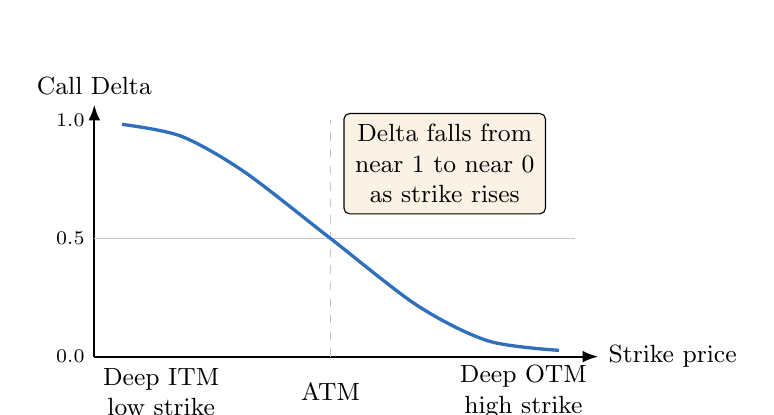
\begin{tikzpicture}[x=1cm,y=1cm,>=Latex]
  \draw[diagramAxis] (0,0) -- (6.4,0) node[right,font=\small]{Strike price};
  \draw[diagramAxis] (0,0) -- (0,3.2) node[above,font=\small]{Call Delta};
  \draw[gray!45] (0,1.5) -- (6.1,1.5);
  \draw[gray!45,dashed] (3,0) -- (3,3);
  \node[left,font=\scriptsize] at (0,3) {1.0};
  \node[left,font=\scriptsize] at (0,1.5) {0.5};
  \node[left,font=\scriptsize] at (0,0) {0.0};
  \draw[diagramBlue,very thick,smooth] plot coordinates {(0.35,2.95) (1.1,2.8) (1.9,2.35) (3,1.5) (4.1,0.65) (5,0.2) (5.9,0.08)};
  \node[font=\small,align=center] at (0.85,-0.45) {Deep ITM\\low strike};
  \node[font=\small,align=center] at (3,-0.45) {ATM};
  \node[font=\small,align=center] at (5.45,-0.45) {Deep OTM\\high strike};
  \node[diagramBox,fill=diagramOrange!10] at (4.45,2.45) {Delta falls from\\near 1 to near 0\\as strike rises};
\end{tikzpicture}
\end{center}


\begin{itemize}[leftmargin=*]
    \item \textbf{Deep ITM calls} \(\rightarrow\) \(\Delta \approx 1.0\) — move nearly dollar-for-dollar with the underlying
    \item \textbf{ATM calls} \(\rightarrow\) \(\Delta \approx 0.50\)
    \item \textbf{Deep OTM calls} \(\rightarrow\) \(\Delta \approx 0\) — barely respond to underlying moves
\end{itemize}

For puts, this is mirrored (deep ITM puts: \(\Delta \approx -1.0\); deep OTM puts: \(\Delta \approx 0\)).

\begin{quote}
Also note: Delta tends to increase in magnitude \emph{closer to expiration} for near/ATM options, because the probability of finishing ITM becomes more binary.
\end{quote}

\subsubsection{Delta in Practice}

\begin{center}
\scriptsize
\setlength{\tabcolsep}{3pt}
\begin{tabular}{|L{3.0cm}|L{3.0cm}|L{3.0cm}|L{3.0cm}|}
\hline
\textbf{Delta Range} & \textbf{Type} & \textbf{Cost} & \textbf{Suitable For} \\
\hline
0.70 – 1.0 & Deep ITM & Expensive & High-conviction directional bets \\
\hline
0.50 & ATM & Moderate & Balanced risk/reward \\
\hline
0.10 – 0.30 & OTM & Cheap & Speculative, high-leverage lottery plays \\
\hline
\end{tabular}
\end{center}

\begin{quote}
\textbf{Caution for new traders:} High-Delta options give bigger dollar moves, but cost more and carry higher risk. Don't chase Delta without understanding the cost.
\end{quote}

\subsection{Gamma (\texorpdfstring{\(\Gamma\)}{Gamma}) — Rate of Change of Delta}

\subsubsection{Definition}

\textbf{Gamma measures how quickly Delta changes for a \$1 move in the underlying asset.} It is the second derivative of the option price with respect to the underlying.

\[
\Gamma = \frac{\partial \Delta}{\partial S} = \frac{\partial^2 V}{\partial S^2}
\]

\textbf{Analogy:} If Delta is the \emph{speed} of an option's price change, Gamma is the \emph{acceleration}.

\textbf{Expressed as:} Change in Delta per \$1 (one-point) move in the underlying.

\textbf{Key properties:}
\begin{itemize}[leftmargin=*]
    \item Gamma is \textbf{always positive} for long options (both calls and puts)
    \item Gamma is \textbf{always negative} for short options
    \item Gamma is \textbf{highest for ATM options}
    \item Gamma \textbf{approaches zero} for deep ITM or deep OTM options
\end{itemize}

\subsubsection{Why Gamma Matters}

Two options with the same Delta but different Gammas will behave very differently when the underlying moves. The one with higher Gamma has a \textbf{more reactive Delta} — directional exposure shifts faster.

\textbf{High Gamma = Delta changes rapidly = larger acceleration of gains (or losses).}

Two options with the same Delta — one high-Gamma, one low-Gamma:
\begin{itemize}[leftmargin=*]
    \item The high-Gamma option has \textbf{higher risk}: an unfavorable move in the underlying will have an outsized impact.
    \item High Gamma values signal that the option tends to experience \textbf{volatile swings} in value.
\end{itemize}

\subsubsection{Gamma Example}

\begin{center}
\scriptsize
\setlength{\tabcolsep}{3pt}
\begin{tabular}{|L{4.1cm}|L{4.1cm}|L{4.1cm}|}
\hline
\textbf{} & \textbf{Before Move} & \textbf{After +\$1 Move} \\
\hline
Underlying price & \(30 | \)31 &  \\
\hline
Option price & \(0.91 | \)1.25 &  \\
\hline
Delta & 0.31 & 0.37 \\
\hline
Gamma & 0.06 & 0.065 \\
\hline
\end{tabular}
\end{center}

\textbf{How we get the new price:}
Since Delta changes over the move, we use the \emph{average} Delta:
\[
\text{Average } \Delta = \frac{0.31 + 0.37}{2} = 0.34
\]
\[
\text{Price change} = 0.34 \times 1 = \$0.34
\]
\[
\text{New price} = 0.91 + 0.34 = \$1.25 \checkmark
\]

\textbf{Delta changed by 0.06 (= Gamma \(\times\) \$1 move).} Notice Gamma itself also shifted from 0.06 to 0.065 — showing that both Delta and Gamma are dynamically changing. Approximations break down for large moves.

\subsubsection{How Gamma Changes with Volatility and Time}

\paragraph{Effect of Implied Volatility on Gamma (at constant time to expiry)}\par\noindent


\begin{center}
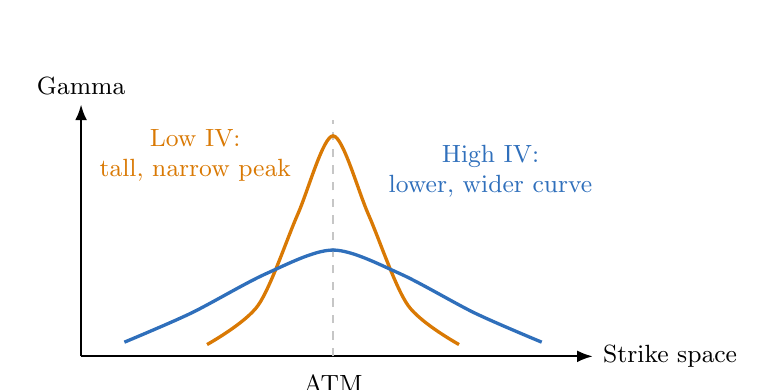
\begin{tikzpicture}[x=1cm,y=1cm,>=Latex]
  \draw[diagramAxis] (0,0) -- (6.5,0) node[right,font=\small]{Strike space};
  \draw[diagramAxis] (0,0) -- (0,3.2) node[above,font=\small]{Gamma};
  \draw[gray!45,dashed] (3.2,0) -- (3.2,3);
  \node[font=\small] at (3.2,-0.35) {ATM};
  \draw[diagramOrange,very thick,smooth] plot coordinates {(1.6,0.15) (2.25,0.65) (2.75,1.8) (3.2,2.8) (3.65,1.8) (4.15,0.65) (4.8,0.15)};
  \draw[diagramBlue,very thick,smooth] plot coordinates {(0.55,0.18) (1.4,0.55) (2.35,1.05) (3.2,1.35) (4.05,1.05) (5,0.55) (5.85,0.18)};
  \node[font=\small,diagramOrange,align=center] at (1.45,2.55) {Low IV:\\tall, narrow peak};
  \node[font=\small,diagramBlue,align=center] at (5.2,2.35) {High IV:\\lower, wider curve};
\end{tikzpicture}
\end{center}


\begin{itemize}[leftmargin=*]
    \item \textbf{Lower IV \(\rightarrow\) Higher Gamma at ATM:} With low IV, expected price movement is concentrated near the current price, making ATM options extremely sensitive.
    \item \textbf{Higher IV \(\rightarrow\) Lower but more spread-out Gamma:} The sensitivity is more distributed across strikes.
    \item This relationship does \emph{not} hold uniformly across all strikes — the curves can cross at strikes far from ATM.
\end{itemize}

\newpage

\paragraph{Effect of Time to Expiry on Gamma (near ATM)}\par\noindent


\begin{center}
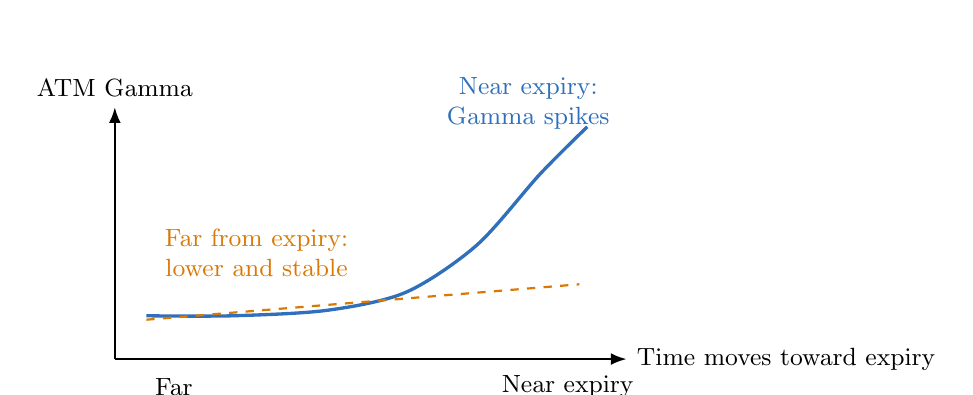
\begin{tikzpicture}[x=1cm,y=1cm,>=Latex]
  \draw[diagramAxis] (0,0) -- (6.5,0) node[right,font=\small]{Time moves toward expiry};
  \draw[diagramAxis] (0,0) -- (0,3.2) node[above,font=\small]{ATM Gamma};
  \draw[diagramBlue,very thick,smooth] plot coordinates {(0.4,0.55) (1.5,0.55) (2.7,0.62) (3.7,0.85) (4.6,1.45) (5.4,2.35) (6,2.95)};
  \draw[diagramOrange,thick,dashed] (0.4,0.5) -- (5.9,0.95);
  \node[font=\small,diagramOrange,align=center] at (1.8,1.35) {Far from expiry:\\lower and stable};
  \node[font=\small,diagramBlue,align=center] at (5.25,3.25) {Near expiry:\\Gamma spikes};
  \node[font=\small] at (0.75,-0.35) {Far};
  \node[font=\small] at (5.75,-0.35) {Near expiry};
\end{tikzpicture}
\end{center}


\begin{itemize}[leftmargin=*]
    \item \textbf{Near expiry:} Gamma is \emph{very high} for ATM options — Deltas can flip almost instantly.
    \item \textbf{Far from expiry:} Gamma is lower and more stable.
    \item \textbf{Intuition:} As expiry approaches, whether an option ends up ITM or OTM becomes increasingly binary — a small move can change everything. Delta is therefore extremely sensitive.
\end{itemize}

\subsubsection{Gamma Scalping — The Core Strategy of Long Gamma}

\textbf{Gamma scalping} is how being long options (long Gamma) generates profits from underlying price moves, independent of direction.

\textbf{Setup:}
\begin{itemize}[leftmargin=*]
    \item Buy 100 call options, each with \(\Delta = 0.31\), \(\Gamma = 0.06\)
    \item Portfolio Delta = \(100 \times 0.31 = +31\)
    \item Delta-hedge by \textbf{selling 31 futures} \(\rightarrow\) net portfolio Delta = 0 (delta-neutral)
\end{itemize}

\textbf{Step 1 — Underlying rises from \$30 \(\rightarrow\) \$31:}
\begin{itemize}[leftmargin=*]
    \item Gamma causes each option's Delta to increase from 0.31 to 0.37
    \item Portfolio Delta from options = \(100 \times 0.37 = +37\)
    \item Net Delta = \(+37 - 31 = +6\) (unhedged, long exposure)
    \item \textbf{Action:} Sell 6 more futures at \textbf{\$31} \(\rightarrow\) re-hedge to Delta = 0
\end{itemize}

\textbf{Step 2 — Underlying falls back \$31 \(\rightarrow\) \$30:}
\begin{itemize}[leftmargin=*]
    \item Delta reverts to 0.31 per option
    \item Portfolio Delta from options = \(+31\), but we now have \(-37\) futures outstanding
    \item Net Delta = \(31 - 37 = -6\) (unhedged, short exposure)
    \item \textbf{Action:} Buy 6 futures at \textbf{\$30} \(\rightarrow\) re-hedge to Delta = 0
\end{itemize}

\textbf{Net result from futures trades:}
\[
\begin{aligned}
&\text{Sold 6 futures at \$31, bought back at \$30} \\
&\implies \text{Profit} = \$1 \times 6 = \$6 \text{ (per multiplier unit)}
\end{aligned}
\]

\begin{quote}
\textbf{The principle:} Being long Gamma means you \emph{gain Deltas in the direction of the underlying's move}. You sell when the underlying rises (high) and buy when it falls (low), mechanically locking in profit on each oscillation.
\end{quote}

\textbf{If you are short options (short Gamma):} You're forced to do the opposite — buy high and sell low — locking in a \textbf{loss} on each oscillation.

\textbf{Why not always be long Gamma?}
Because long options decay in value with the passage of time (\textbf{Theta}). The profit from Gamma scalping must exceed the daily cost of time decay. This is the eternal struggle at the heart of options trading:

\[
\boxed{\text{P\&L (long option)} = \underbrace{\text{Gamma scalping profit}}_{\text{from underlying moves}} - \underbrace{\text{Theta cost}}_{\text{daily time decay}}}
\]

\subsubsection{Gamma: Friend or Enemy?}

\begin{center}
\scriptsize
\setlength{\tabcolsep}{3pt}
\begin{tabular}{|L{4.1cm}|L{4.1cm}|L{4.1cm}|}
\hline
\textbf{Scenario} & \textbf{Long Gamma (option buyer)} & \textbf{Short Gamma (option seller)} \\
\hline
Underlying moves in your favor & \(\checkmark\) Profits accelerate & \(\times\) Losses accelerate \\
\hline
Underlying moves against you & \(\checkmark\) Losses decelerate & \(\times\) Losses accelerate \\
\hline
Underlying barely moves & \(\times\) Lose Theta each day & \(\checkmark\) Collect Theta each day \\
\hline
\end{tabular}
\end{center}

\subsection{Theta (\texorpdfstring{\(\Theta\)}{Theta}) — Time Decay}

\subsubsection{Definition}

\textbf{Theta measures the rate of time decay of an option — how much the option's price decreases over one trading day, with all other inputs held constant (underlying price, IV, interest rates, etc.).}

\[
\Theta = \frac{\partial V}{\partial t}
\]

\begin{itemize}[leftmargin=*]
    \item Theta is \textbf{always negative} for long options — the option buyer's position loses value each day.
    \item Theta is \textbf{always positive} for short options — the option seller's position gains value as the option decays.
    \item Expressed in \textbf{dollars (or cents) per 24-hour period}.
\end{itemize}

\textbf{Traders' terminology:}
\begin{itemize}[leftmargin=*]
    \item \textbf{"Paying theta"} = you are long an option; you pay the decay cost every day you hold it.
    \item \textbf{"Collecting theta"} = you are short an option; you gain as the option price decays.
\end{itemize}

\begin{quote}
Theta is generally \textbf{good for sellers, bad for buyers.}
\end{quote}

\subsubsection{Example of Theta}

Consider a call option with a theta of \$-0.12 (i.e., 12 cents per day). This means:

\[
\text{New option price (next day)} = \text{Current price} - 0.12
\]

From an S\&P 500 Dec 930 ATM call option (all else equal):

\begin{center}
\scriptsize
\setlength{\tabcolsep}{3pt}
\begin{tabular}{|L{6.3cm}|L{6.3cm}|}
\hline
\textbf{Time} & \textbf{Daily Theta (\$/day lost)} \\
\hline
T+0 (position opened) & \$45.40 \\
\hline
T+6 & \$51.85 \\
\hline
T+13 & \$65.20 \\
\hline
T+19 (6 days to expiry) & \$93.30 \\
\hline
\end{tabular}
\end{center}

The option loses value faster and faster as expiration approaches.

\subsubsection{Time Decay Acceleration}

Theta does \textbf{not} decay linearly — it \textbf{accelerates}, particularly for ATM options:


\begin{center}
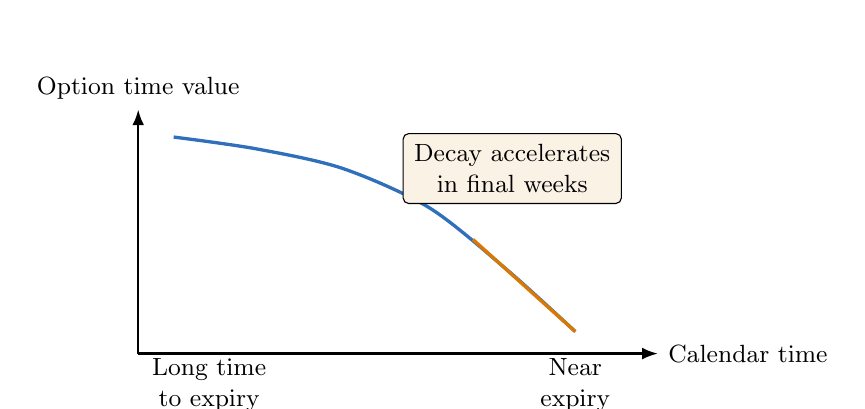
\begin{tikzpicture}[x=1cm,y=1cm,>=Latex]
  \draw[diagramAxis] (0,0) -- (6.6,0) node[right,font=\small]{Calendar time};
  \draw[diagramAxis] (0,0) -- (0,3.1) node[above,font=\small]{Option time value};
  \draw[diagramBlue,very thick,smooth] plot coordinates {(0.45,2.75) (1.5,2.6) (2.6,2.35) (3.7,1.85) (4.7,1.05) (5.55,0.28)};
  \draw[diagramOrange,very thick] (4.25,1.45) -- (5.55,0.28);
  \node[font=\small,align=center] at (0.9,-0.4) {Long time\\to expiry};
  \node[font=\small,align=center] at (5.55,-0.4) {Near\\expiry};
  \node[diagramBox,fill=diagramOrange!10] at (4.75,2.35) {Decay accelerates\\in final weeks};
\end{tikzpicture}
\end{center}


\begin{itemize}[leftmargin=*]
    \item \textbf{ATM options:} Retain the most time value until late, then Theta accelerates sharply in the final weeks.
    \item \textbf{Deep ITM and OTM options:} Their extrinsic value is already low near expiry, so the slope flattens — less dramatic acceleration.
\end{itemize}

\begin{quote}
For OTM options with high implied volatility, Theta can also be quite high — reflecting the significant time value embedded in their premiums.
\end{quote}

\subsubsection{Theta Across Strike Space}


\begin{center}
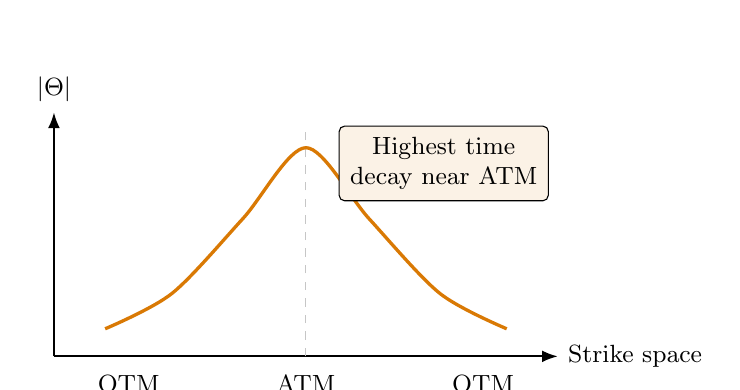
\begin{tikzpicture}[x=1cm,y=1cm,>=Latex]
  \draw[diagramAxis] (0,0) -- (6.4,0) node[right,font=\small]{Strike space};
  \draw[diagramAxis] (0,0) -- (0,3.1) node[above,font=\small]{\(|\Theta|\)};
  \draw[gray!45,dashed] (3.2,0) -- (3.2,2.9);
  \draw[diagramOrange,very thick,smooth] plot coordinates {(0.65,0.35) (1.5,0.8) (2.4,1.75) (3.2,2.65) (4,1.75) (4.9,0.8) (5.75,0.35)};
  \node[font=\small] at (3.2,-0.35) {ATM};
  \node[font=\small] at (0.95,-0.35) {OTM};
  \node[font=\small] at (5.45,-0.35) {OTM};
  \node[diagramBox,fill=diagramOrange!10] at (4.95,2.45) {Highest time\\decay near ATM};
\end{tikzpicture}
\end{center}


\begin{itemize}[leftmargin=*]
    \item \textbf{ATM options have the highest Theta} — they carry the most time value, so there's more to decay.
    \item OTM options have less time value; ITM options have more intrinsic value — both have less Theta than ATM.
\end{itemize}

\textbf{Theta through time for different strikes:}
\begin{itemize}[leftmargin=*]
    \item \textbf{OTM options:} Theta actually \emph{decreases} as we approach expiry (less extrinsic value remains)
    \item \textbf{ATM options:} Theta \emph{increases} as we approach expiry (the familiar acceleration)
\end{itemize}

This causes the Theta curves across strikes to \emph{cross over} at different points in time.

\subsubsection{Theta vs. Gamma: The Eternal Trade-Off}

This is the central tension in options trading for every buyer and seller:

\textbf{From the earlier example:}
\begin{center}
\scriptsize
\setlength{\tabcolsep}{3pt}
\begin{tabular}{|L{4.1cm}|L{4.1cm}|L{4.1cm}|}
\hline
\textbf{} & \textbf{Calculation} & \textbf{Result} \\
\hline
\textbf{Theta cost} & \(12 \text{ cents} \times 100 \text{ options} \times 100 \text{ (multiplier)}\) & \(-\$1,200/\text{day}\) \\
\hline
\textbf{Gamma scalping profit} & \(6 \text{ futures} \times \$1 \times 100 \text{ (multiplier)}\) & \(+\$600\) \\
\hline
\textbf{Net P\&L} &  & \(-\$600\) (loss) \\
\hline
\end{tabular}
\end{center}

Here, the underlying didn't move \emph{enough} to overcome the time decay. The fundamental question every option buyer must answer:

\begin{quote}
\textbf{Does the P\&L from the underlying's movements exceed the daily cost of time decay (Theta)?}
\end{quote}

If the underlying moves a lot \(\rightarrow\) Gamma scalping profit may dominate \(\rightarrow\) long option is profitable.
If the underlying barely moves \(\rightarrow\) Theta cost dominates \(\rightarrow\) long option loses money.

The market prices options such that, \emph{in expectation}, these two forces balance out at fair value.

\subsection{Vega (\texorpdfstring{\(\nu\)}{nu}) — Sensitivity to Implied Volatility}

\subsubsection{Definition}

\textbf{Vega measures the sensitivity of an option's price to a 1-point change in implied volatility (IV).}

\[
\nu = \frac{\partial V}{\partial \sigma}
\]

where \(\sigma\) = implied volatility.

\begin{quote}
\textbf{Note:} Vega is not actually a Greek letter — it's a word adopted by convention. Despite this, it is one of the most closely watched measures, especially by market makers, since they are essentially \emph{traders of volatility}.
\end{quote}

\textbf{Key properties:}
\begin{itemize}[leftmargin=*]
    \item \textbf{All options have positive Vega} — whether call or put, owning an option means you benefit when IV rises.
    \item \textbf{Vega is identical for a call and put on the same strike} (follows from put-call parity).
    \item Option buyers (long) have \textbf{positive Vega} — they profit when IV rises.
    \item Option sellers (short) have \textbf{negative Vega} — they lose when IV rises.
    \item Vega \textbf{falls as options approach expiration}.
    \item Higher volatility raises option prices regardless of direction — both calls and puts become more expensive.
\end{itemize}

\subsubsection{Vega Example}

A call option with:
\begin{itemize}[leftmargin=*]
    \item Price: \(\$1.00\)
    \item Delta: \$0.30\$
    \item Vega: \$0.04\$
    \item Current implied volatility: \(15\%\)
\end{itemize}

\textbf{If IV increases from 15\% to 16\% (+1 point):}
\[
\text{New option price} = \$1.00 + 0.04 \times 1 = \$1.04
\]

\textbf{If IV increases from 15\% to 16.1\% (+1.1 points):}
\[
\text{New option price} = \$1.00 + 0.04 \times 1.1 = \$1.044
\]

This is a \textbf{linear relationship}: option price changes proportionally with IV changes.

\textbf{Portfolio-level Vega:}
Holding 100 call options (multiplier = 1,000):

\[
\text{P\&L change per 1-pt IV move} = 0.04 \times 100 \times 1000 = \$4{,}000
\]

Traders express this as: \textbf{"I'm long 4 Vegas"} or \textbf{"long \$4,000 Vega"} — meaning a 1-point rise in IV earns \$4,000, and a 1-point fall costs \$4,000.

A seller of the same 100 options would lose \$4,000 for every 1-point rise in IV (short Vega = negative exposure).

\subsubsection{Vega Across Strike Space}


\begin{center}
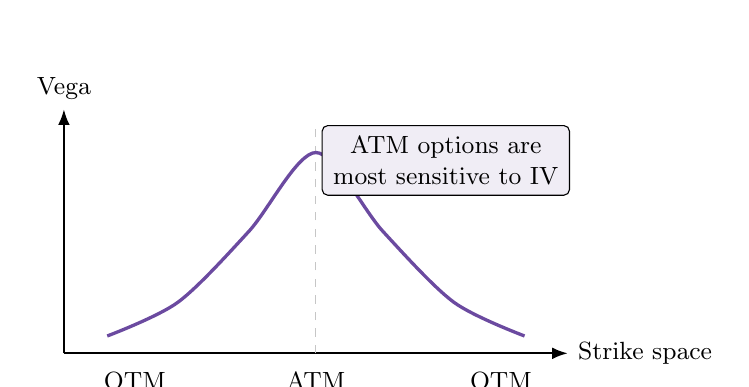
\begin{tikzpicture}[x=1cm,y=1cm,>=Latex]
  \draw[diagramAxis] (0,0) -- (6.4,0) node[right,font=\small]{Strike space};
  \draw[diagramAxis] (0,0) -- (0,3.1) node[above,font=\small]{Vega};
  \draw[gray!45,dashed] (3.2,0) -- (3.2,2.9);
  \draw[diagramPurple,very thick,smooth] plot coordinates {(0.55,0.22) (1.45,0.65) (2.35,1.55) (3.2,2.55) (4.05,1.55) (4.95,0.65) (5.85,0.22)};
  \node[font=\small] at (3.2,-0.35) {ATM};
  \node[font=\small] at (0.9,-0.35) {OTM};
  \node[font=\small] at (5.55,-0.35) {OTM};
  \node[diagramBox,fill=diagramPurple!10] at (4.85,2.45) {ATM options are\\most sensitive to IV};
\end{tikzpicture}
\end{center}


\begin{itemize}[leftmargin=*]
    \item \textbf{ATM options have the highest Vega} — their prices are most sensitive to changes in IV.
    \item Moving away from ATM in either direction reduces Vega.
    \item In practice, the curve may be slightly \textbf{asymmetric} due to \textbf{volatility skew} (different IV levels priced into different strikes — OTM puts typically have higher IV than OTM calls).
\end{itemize}

\subsubsection{Effect of Time to Expiry on Vega}


\begin{center}
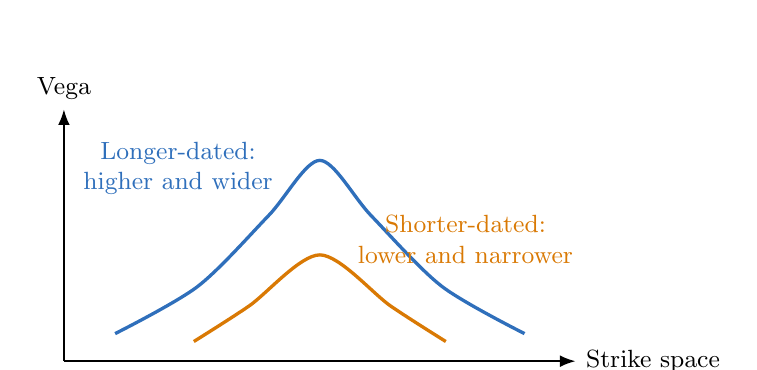
\begin{tikzpicture}[x=1cm,y=1cm,>=Latex]
  \draw[diagramAxis] (0,0) -- (6.5,0) node[right,font=\small]{Strike space};
  \draw[diagramAxis] (0,0) -- (0,3.2) node[above,font=\small]{Vega};
  \draw[diagramBlue,very thick,smooth] plot coordinates {(0.65,0.35) (1.7,0.95) (2.6,1.85) (3.25,2.55) (3.9,1.85) (4.8,0.95) (5.85,0.35)};
  \draw[diagramOrange,very thick,smooth] plot coordinates {(1.65,0.25) (2.35,0.7) (3.25,1.35) (4.15,0.7) (4.85,0.25)};
  \node[font=\small,diagramBlue,align=center] at (1.45,2.45) {Longer-dated:\\higher and wider};
  \node[font=\small,diagramOrange,align=center] at (5.1,1.55) {Shorter-dated:\\lower and narrower};
\end{tikzpicture}
\end{center}


\textbf{Longer-dated options have higher Vega} — a change in expected volatility has a larger impact when there's more time for that volatility to affect the final outcome.

\textbf{As options approach expiry, Vega decreases} — there's less time for IV changes to matter.

This is why options traders say: \textbf{"Longer-dated options are more expensive to volatility moves."}

\subsubsection{Effect of IV Level on Vega}

When the overall level of implied volatility decreases:
\begin{itemize}[leftmargin=*]
    \item The Vega of all options \textbf{decreases} (options become less sensitive to further IV changes).
    \item Intuitively: when IV is already low, a 1-point change is a larger \emph{relative} change, but the absolute dollar sensitivity of the option is lower.
\end{itemize}

\subsubsection{Long vs. Short Vega: Practical Implications}

\begin{center}
\scriptsize
\setlength{\tabcolsep}{3pt}
\begin{tabular}{|L{4.1cm}|L{4.1cm}|L{4.1cm}|}
\hline
\textbf{Position} & \textbf{IV Rises} & \textbf{IV Falls} \\
\hline
Long call / long put (long Vega) & \(\checkmark\) Profit & \(\times\) Loss \\
\hline
Short call / short put (short Vega) & \(\times\) Loss & \(\checkmark\) Profit \\
\hline
\end{tabular}
\end{center}

\textbf{When is Vega most important?}
\begin{itemize}[leftmargin=*]
    \item \textbf{Earnings seasons and major news events} — IV typically spikes before the event ("volatility bid up") and then collapses immediately after ("IV crush" or "volatility crush").
    \item Option buyers benefit from rising IV \emph{before} the event; option sellers benefit from the collapse \emph{after}.
\end{itemize}

\textbf{Vega-neutral positions:} Traders can combine options to make their portfolio insensitive to IV changes (vega-neutral), isolating other risks.

\subsection{Rho (\texorpdfstring{\(\rho\)}{rho}) — Sensitivity to Interest Rates}

\textbf{Rho measures how much an option's price changes with a 1\% change in the risk-free interest rate.}

\[
\rho = \frac{\partial V}{\partial r}
\]

\begin{itemize}[leftmargin=*]
    \item \textbf{Call options have positive Rho} — they gain value when interest rates rise.
    \item \textbf{Put options have negative Rho} — they lose value when interest rates rise.
    \item Rho is generally the \textbf{least impactful Greek} in normal conditions.
    \item Becomes \textbf{more significant for long-term options (LEAPS)} and during periods of significant monetary policy changes (e.g., rapid rate hike or cut cycles).
\end{itemize}

\textbf{Intuition:} Higher interest rates increase the opportunity cost of holding the underlying stock. Call options become relatively more attractive than holding the stock outright (since you can invest the cash instead and use the cheaper call as a proxy), increasing their value. Conversely, the benefit of holding puts to hedge is reduced.

\subsection{Key Relationships to Remember}

\textbf{1. Delta and Gamma:}
Gamma tells you how Delta will change. High Gamma means Delta can shift rapidly — critical for risk management, especially near expiry.

\textbf{2. Gamma and Theta (The Central Trade-off):}
Long options = long Gamma + short Theta. Short options = short Gamma + long Theta.
The market prices options so that, \emph{in expectation}, the Gamma profit from underlying moves equals the Theta cost over time.

\textbf{3. Vega and Time:}
Longer-dated options have higher Vega — more sensitive to IV changes. As expiry nears, Vega falls.

\textbf{4. Delta, Volatility, and Time:}
Increasing IV \emph{or} increasing time to expiry both push all option Deltas toward 0.50.
Decreasing IV \emph{or} decreasing time push OTM Deltas toward 0 and ITM Deltas toward \(\pm\)1.

\textbf{5. Put-Call Relationships (from Put-Call Parity):}
For the same strike and expiry:
\[
|\Delta_{\text{call}}| + |\Delta_{\text{put}}| = 1
\]
\[
\nu_{\text{call}} = \nu_{\text{put}} \quad (\text{Vega is equal})
\]
\[
|\Theta_{\text{call}}| \approx |\Theta_{\text{put}}| \quad (\text{Theta is equal in magnitude})
\]
\[
\Gamma_{\text{call}} = \Gamma_{\text{put}} \quad (\text{Gamma is equal})
\]

\section{Volatility and its Effect on Option Prices}

\subsection{What Is Volatility?}

\textbf{Volatility} is a measure of the rate of fluctuation in the price of a security over time. It captures how much and how rapidly prices change — the higher the volatility, the more uncertain and risky the security.

Two common ways to measure it:

\begin{itemize}[leftmargin=*]
    \item \textbf{Standard Deviation:} Measures the dispersion of a security's historical prices around its mean price. This is the most common approach.
    \item \textbf{Beta (\(\beta\)):} Measures a security's volatility \emph{relative to the overall market} (typically the S\&P 500). Calculated via regression analysis. A \(\beta\) of 1.5 means the stock is theoretically 50\% more volatile than the market.
\end{itemize}

\begin{quote}
\textbf{Why it matters for options:} Volatility is one of the primary inputs to option pricing models (e.g., Black-Scholes). The higher the volatility, the greater the probability that the underlying price will move enough to reach (or exceed) the strike price — making options more valuable.
\end{quote}

\subsection{Types of Volatility}

\subsubsection{Historical Volatility (HV) — also called Statistical Volatility}

\textbf{Historical volatility measures fluctuations in a security's price over a past time period.}

\begin{itemize}[leftmargin=*]
    \item Computed from past price data using statistical methods (standard deviation).
    \item Often calculated annually, but can be computed daily or for shorter windows.
    \item Useful for understanding how volatile a security \emph{has been}.
    \item \textbf{Key limitation:} It tells you nothing about the \emph{direction} of future price movement — only the magnitude of past moves.
\end{itemize}

\begin{quote}
Generally, a higher historical volatility percentage translates to a higher option value.
HV is also thought to be \textbf{mean-reverting} over the long run: if observed HV is far above the security's fundamental average level, it tends to fall back; if far below, it tends to rise.
\end{quote}

\subsubsection{Implied Volatility (IV)}

\textbf{Implied volatility is the market's forward-looking expectation of how much the underlying asset will move over the option's remaining life.}

\begin{itemize}[leftmargin=*]
    \item Rather than computed from historical prices, IV is \textbf{inferred from the market price of the option itself} — by back-solving the Black-Scholes model for the volatility input that produces the observed option premium.
    \item Since option prices are publicly observable, IV gives a real-time, consensus view of expected future price movement.
    \item It is \textbf{forward-looking}, not backward-looking like HV.
    \item Every option (call or put, every strike, every expiry) has its own IV — and these can differ across strikes (\(\rightarrow\) \textbf{skew}) and across expiries (\(\rightarrow\) \textbf{term structure}).
\end{itemize}

\textbf{Relationship between IV and market direction:}
\begin{itemize}[leftmargin=*]
    \item When options markets experience a \textbf{downtrend} (market fear rises), IV generally \textbf{increases} — investors demand more protection (puts), bidding up premiums.
    \item When markets are in an \textbf{uptrend} (calm), IV generally \textbf{falls} — less demand for protection.
\end{itemize}

\textbf{Mathematically:}

The option price from Black-Scholes can be written as:

\[
C = f(S,\ K,\ T,\ r,\ \sigma)
\]

where \(\sigma\) is volatility. Implied volatility \(\sigma_{IV}\) is found by solving:

\[
C_{\text{market}} = f(S,\ K,\ T,\ r,\ \sigma_{IV})
\]

This must be solved numerically (no closed form). Trading platforms do this automatically.

\subsection{Calculating Historical Volatility}

\subsubsection{Step-by-Step (Standard Deviation Method)}

\begin{enumerate}[leftmargin=*]
    \item Gather the security's past prices over the chosen period.
    \item Calculate the \textbf{mean price} \(\bar{P}\).
    \item Find the \textbf{difference} between each price and the mean: \((P_i - \bar{P})\).
    \item \textbf{Square} each difference: \((P_i - \bar{P})^2\).
    \item \textbf{Sum} the squared differences.
    \item Divide by the number of observations to get the \textbf{variance}: \(\sigma^2 = \frac{\sum(P_i - \bar{P})^2}{N}\).
    \item Take the \textbf{square root} to get the \textbf{standard deviation (volatility)}: \(\sigma = \sqrt{\sigma^2}\).
\end{enumerate}

\[
\boxed{\sigma = \sqrt{\frac{\sum_{i=1}^{N}(P_i - \bar{P})^2}{N}}}
\]

\subsubsection{Worked Example}

Stock prices of ABC Corp. over 4 days: \$10, \$12, \$9, \$14.

\begin{center}
\scriptsize
\setlength{\tabcolsep}{3pt}
\begin{tabular}{|L{4.1cm}|L{4.1cm}|L{4.1cm}|}
\hline
\textbf{Step} & \textbf{Calculation} & \textbf{Result} \\
\hline
Mean price & \((10 + 12 + 9 + 14) / 4\) & \(\bar{P} = \$11.25\) \\
\hline
Deviations & \(10-11.25,\ 12-11.25,\ 9-11.25,\ 14-11.25\) & \(-1.25,\ 0.75,\ -2.25,\ 2.75\) \\
\hline
Squared deviations & \(\begin{gathered}(-1.25)^2,\ (0.75)^2,\\(-2.25)^2,\ (2.75)^2\end{gathered}\) & \(\begin{gathered}1.5625,\ 0.5625,\\5.0625,\ 7.5625\end{gathered}\) \\
\hline
Sum of squared deviations & \(1.56 + 0.56 + 5.06 + 7.56\) & \(14.75\) \\
\hline
Variance & \(14.75 / 4\) & \(\sigma^2 = 3.6875\) \\
\hline
\textbf{Standard deviation} & \(\sqrt{3.69}\) & \(\sigma \approx \mathbf{\$1.92}\) \\
\hline
\end{tabular}
\end{center}

\textbf{Interpretation:} The stock price of ABC Corp. typically deviates from its mean by about \$1.92 per day.

\subsubsection{Annualizing Volatility}

Daily volatility must be annualized for use in options pricing. The standard approach:

\[
\sigma_{\text{annual}} = \sigma_{\text{daily}} \times \sqrt{T}
\]

where \(T\) = number of trading days per year.

\begin{itemize}[leftmargin=*]
    \item Convention: \textbf{252 trading days/year} \(\rightarrow\) \(\sqrt{252} \approx 15.87\)
    \item Some traders use \textbf{256 trading days} because \(\sqrt{256} = 16\) exactly — a convenient multiplier.
\end{itemize}

\[
\boxed{\sigma_{\text{annual}} = \sigma_{\text{daily}} \times 16}
\]

\subsection{Implied Volatility and Option Pricing}

\subsubsection{IV and Option Premiums}

The relationship is direct and applies universally:

\begin{quote}
\textbf{As IV rises, the prices of ALL options on that underlying — both calls and puts, at ALL strike prices — increase.}
\end{quote}

This is because higher expected volatility means greater probability of any given strike being reached before expiry, increasing the option's chance of being ITM.

\begin{itemize}[leftmargin=*]
    \item Higher IV \(\rightarrow\) higher option premiums \(\rightarrow\) \textbf{benefits option buyers} (long Vega)
    \item Lower IV \(\rightarrow\) cheaper premiums \(\rightarrow\) \textbf{benefits option sellers} (short Vega)
\end{itemize}

\textbf{How to use this practically:}
\begin{itemize}[leftmargin=*]
    \item Buy options when IV is \textbf{low} (premiums are cheap) — you expect volatility to rise.
    \item Sell options when IV is \textbf{high} (premiums are expensive) — you expect volatility to collapse.
\end{itemize}

\begin{quote}
\textbf{Smart hedging principle:} Astute investors buy put options (for portfolio protection) when the VIX (and thus IV) is relatively \textbf{low} and put premiums are cheap — like buying insurance before a storm rather than during one.
\end{quote}

\subsubsection{IV and Delta}

Increasing IV doesn't just raise option prices — it also affects Delta:

\begin{quote}
\textbf{As IV increases, the Deltas of all options — calls and puts, at all strikes — move toward 0.50.}
\end{quote}

\begin{itemize}[leftmargin=*]
    \item OTM option Deltas rise (approaching 0.50) — more chance of reaching the strike.
    \item ITM option Deltas fall toward 0.50 — less certainty they'll stay ITM.
\end{itemize}

This makes sense: higher expected volatility means outcomes are more uncertain, so the probability of finishing ITM or OTM becomes closer to 50/50 for all strikes.

\subsubsection{IV and Option Price Decomposition}

Recall that an option's premium has two components:

\[
\text{Option Premium} = \underbrace{\text{Intrinsic Value}}_{\text{max}(S-K, 0) \text{ for call}} + \underbrace{\text{Time/Extrinsic Value}}_{\text{depends on IV, time, etc.}}
\]

IV affects the \textbf{extrinsic (time) value} directly. A higher IV inflates the time value of both calls and puts at every strike.

\subsection{The VIX — CBOE Volatility Index}

\subsubsection{What Is the VIX?}

The \textbf{CBOE Volatility Index (VIX)} — also called the \textbf{"Fear Index"} — is a real-time index measuring the market's expectation of \textbf{30-day forward volatility of the S\&P 500}, derived from live S\&P 500 index option (SPX) prices.

\begin{quote}
The VIX represents implied volatility (IV) for the broad U.S. equity market. It does not measure the S\&P 500's actual past movements — it represents \emph{what options markets imply} about future movements.
\end{quote}

\textbf{Key facts:}
\begin{itemize}[leftmargin=*]
    \item Created by the \textbf{CBOE Global Markets}, introduced in \textbf{1993}.
    \item In \textbf{2003}, methodology was updated in collaboration with \textbf{Goldman Sachs} to use the broader S\&P 500 (instead of the original S\&P 100), increasing accuracy.
    \item Calculated in \textbf{real-time} during market hours (3:00 AM – 4:15 PM EST), and since April 2016, also outside U.S. trading hours.
\end{itemize}

\subsubsection{How Is the VIX Calculated?}

The VIX uses a portfolio of \textbf{SPX options} (both puts and calls, across many strike prices) that expire between \textbf{23 and 37 days from today}. Specifically:
\begin{itemize}[leftmargin=*]
    \item \textbf{Standard SPX options} (expire 3rd Friday of each month)
    \item \textbf{Weekly SPX options} (expire all other Fridays)
\end{itemize}

The formula averages the \textbf{weighted prices} of qualifying SPX puts and calls across a wide range of strikes, theoretically estimating the expected 30-day volatility of the S\&P 500.

\[
\text{VIX} \approx \sqrt{\frac{2}{T} \sum_i \frac{\Delta K_i}{K_i^2} e^{rT} Q(K_i) - \frac{1}{T}\left(\frac{F}{K_0} - 1\right)^2} \times 100
\]

where \(Q(K_i)\) is the midpoint of the bid-ask spread for an option at strike \(K_i\), \(F\) is the forward price, \(T\) is time to expiration, and \(r\) is the risk-free rate. (The detailed derivation is in the CBOE VIX white paper.)

\begin{quote}
\textbf{In plain terms:} VIX is the expected annualized move (in \%) of the S\&P 500 over the next 30 days, implied by option prices. A VIX of 20 means options are pricing in roughly a \(\pm\)20\% annualized move.
\end{quote}

\subsubsection{Interpreting VIX Levels}

\begin{center}
\scriptsize
\setlength{\tabcolsep}{3pt}
\begin{tabular}{|L{6.3cm}|L{6.3cm}|}
\hline
\textbf{VIX Level} & \textbf{Market Interpretation} \\
\hline
\textbf{\(<\) 20} & Calm, stable market — low fear, low uncertainty \\
\hline
\textbf{20 – 30} & Moderate concern — some tension or uncertainty \\
\hline
\textbf{\(>\) 30} & High fear — significant volatility, uncertainty, or crisis \\
\hline
\textbf{Long-run average} & ~21 (historical baseline) \\
\hline
\end{tabular}
\end{center}

\subsubsection{VIX and the S\&P 500 — The Inverse Relationship}

The S\&P 500 and VIX typically move in \textbf{opposite directions}:


\begin{center}
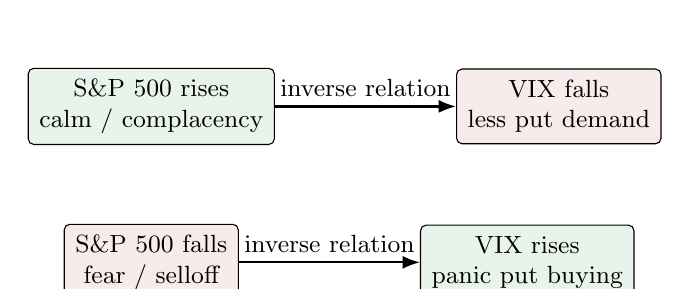
\begin{tikzpicture}[node distance=1.5cm,>=Latex]
  \node[diagramBox,fill=diagramGreen!10] (spup) {S\&P 500 rises\\calm / complacency};
  \node[diagramBox,fill=bearc!10,right=2.3cm of spup] (vixdown) {VIX falls\\less put demand};
  \draw[diagramArrow] (spup) -- node[above,font=\small]{inverse relation} (vixdown);
  \node[diagramBox,fill=bearc!10,below=1.0cm of spup] (spdown) {S\&P 500 falls\\fear / selloff};
  \node[diagramBox,fill=diagramGreen!10,right=2.3cm of spdown] (vixup) {VIX rises\\panic put buying};
  \draw[diagramArrow] (spdown) -- node[above,font=\small]{inverse relation} (vixup);
\end{tikzpicture}
\end{center}


\textbf{Why?} When markets fall, investors rush to buy put options for protection. This surge in demand bids up option premiums, inflating IV — and therefore the VIX. Markets also tend to \textbf{fall fast and rise slowly}: sharp, rapid selloffs create more volatility than gradual gains.

This negative correlation makes VIX-linked instruments useful for \textbf{portfolio hedging} and \textbf{diversification} — they tend to gain when your equity portfolio loses.

\subsubsection{Trading the VIX}

The VIX \textbf{cannot be bought or sold directly} — it is a calculated index, not a tradable asset. However, exposure can be obtained through:

\begin{center}
\scriptsize
\setlength{\tabcolsep}{3pt}
\begin{tabular}{|L{6.3cm}|L{6.3cm}|}
\hline
\textbf{Instrument} & \textbf{Examples} \\
\hline
\textbf{Futures} & CBOE VIX futures (launched March 2004) \\
\hline
\textbf{Options} & VIX options (launched February 2006) \\
\hline
\textbf{ETFs/ETNs} & ProShares VIX Short-Term Futures ETF (VIXY), iPath S\&P 500 VIX STF ETN (VXX) \\
\hline
\end{tabular}
\end{center}

These products allow "pure volatility exposure" — a new, distinct asset class. Hedge funds and institutional investors use them to hedge equity downside and diversify portfolios.

\begin{quote}
\textbf{Beta and VIX in trading:} Traders pricing options on high-beta stocks use VIX values proportionally. For a stock with \(\beta\) = 1.5, the implied volatility would be approximately 1.5\(\times\) the market-wide volatility implied by VIX.
\end{quote}

\subsubsection{VIX Variants}

\begin{center}
\scriptsize
\setlength{\tabcolsep}{3pt}
\begin{tabular}{|L{6.3cm}|L{6.3cm}|}
\hline
\textbf{Index} & \textbf{Measures} \\
\hline
\textbf{VXST} (CBOE Short-Term VI) & 9-day expected volatility of S\&P 500 \\
\hline
\textbf{VXV} (CBOE S\&P 500 3-Month VI) & 3-month expected volatility \\
\hline
\textbf{VXMT} (CBOE S\&P 500 6-Month VI) & 6-month expected volatility \\
\hline
\textbf{VXN} & Nasdaq-100 volatility \\
\hline
\textbf{VXD} & DJIA volatility \\
\hline
\textbf{RVX} & Russell 2000 volatility \\
\hline
\end{tabular}
\end{center}

\subsection{Fear and Greed Index}

\subsubsection{What Is It?}

The \textbf{Fear and Greed Index}, developed by \textbf{CNNMoney}, gauges overall investor sentiment on the stock market using a composite of seven market indicators. It ranges from \textbf{0 (extreme fear)} to \textbf{100 (extreme greed)}.

\[
\text{Index} = \text{Equal-weighted average of 7 sub-indicators, each scored 0–100}
\]

It functions as a \textbf{contrarian indicator}:
\begin{itemize}[leftmargin=*]
    \item When investors are fearful, they sell stocks — possibly below intrinsic value \(\rightarrow\) \textbf{Fear = buy signal}
    \item When investors are greedy, they buy stocks — possibly above intrinsic value \(\rightarrow\) \textbf{Greed = sell signal}
\end{itemize}

\textbf{Scale:}

\begin{center}
\scriptsize
\setlength{\tabcolsep}{3pt}
\begin{tabular}{|L{6.3cm}|L{6.3cm}|}
\hline
\textbf{Value} & \textbf{Sentiment} \\
\hline
0 – 49 & Fear \\
\hline
50 & Neutral \\
\hline
51 – 100 & Greed \\
\hline
\end{tabular}
\end{center}

\begin{quote}
\textbf{Warren Buffett's wisdom:} \emph{"Be fearful when others are greedy, and greedy when others are fearful."}
\end{quote}

\subsubsection{The Seven Factors}

Each factor is independently scored 0–100 and equally weighted:

\begin{center}
\scriptsize
\setlength{\tabcolsep}{3pt}
\begin{tabular}{|L{2.25cm}|L{2.25cm}|L{2.25cm}|L{2.25cm}|L{2.25cm}|}
\hline
\textbf{\#} & \textbf{Factor} & \textbf{Measures} & \textbf{Greed signal} & \textbf{Fear signal} \\
\hline
1 & \textbf{Stock Price Strength} & NYSE stocks at 52-week highs vs. 52-week lows & More highs & More lows \\
\hline
2 & \textbf{Stock Price Breadth} & Trading volume of rising vs. declining NYSE stocks & Rising volume \(>\) declining & Declining volume \(>\) rising \\
\hline
3 & \textbf{Market Momentum} & S\&P 500 vs. its 125-day moving average & S\&P above average & S\&P below average \\
\hline
4 & \textbf{Put/Call Ratio} & CBOE put-to-call ratio & Low P/C ratio & High P/C ratio \\
\hline
5 & \textbf{Safe Haven Demand} & Stocks vs. bonds performance & Stocks outperforming bonds & Bonds outperforming stocks \\
\hline
6 & \textbf{Junk Bond Demand} & Yield spread: investment-grade vs. junk bonds & Narrow spread (high demand for junk) & Wide spread (flight to quality) \\
\hline
7 & \textbf{Market Volatility} & VIX level & Low VIX & High VIX \\
\hline
\end{tabular}
\end{center}

\subsubsection{How to Use It}

The index is primarily a \textbf{market-timing tool}, not a fundamental research tool.

\begin{itemize}[leftmargin=*]
    \item \textbf{Index near 90–100 (extreme greed):} Stocks may be overvalued \(\rightarrow\) consider selling.
    \item \textbf{Index near 0–10 (extreme fear):} Stocks may be undervalued \(\rightarrow\) consider buying.
\end{itemize}

\textbf{Practical example:} On September 29, 2008 (Dow down 778 points / 7\%), the index likely read ~20 (extreme fear). A value of 95 signals extreme greed — not an entry point for a contrarian investor.

\begin{quote}
\textbf{Caveat:} The index is best used as a \emph{secondary} signal alongside fundamental analysis, not as a standalone trading system. Even Buffett's maxim requires knowing \emph{what} you're greedy or fearful about.
\end{quote}

\subsection{Volatility Skew}

\subsubsection{What Is Skew?}

In a world of \textbf{constant IV} — where every option on the same underlying, at every strike price and expiry, had the same implied volatility — the option price distribution across strikes would be \textbf{perfectly symmetric}. An OTM call and an OTM put equidistant from the current price would cost the same.

In reality, this is never the case. \textbf{Volatility skew} refers to the fact that options at different strike prices on the same underlying trade at \textbf{different implied volatilities}.

\begin{quote}
The essential observation: IV is not uniform across all options on the same underlying.
\end{quote}

\subsubsection{Why Does Skew Exist? — Supply and Demand Imbalances}

Skew is entirely a market phenomenon driven by \textbf{supply and demand imbalances} for options at different strikes.

\textbf{For the S\&P 500 (and most equity indices), the dominant pattern is \emph{negative skew}:}

\textbf{Reason 1 — Asymmetric market behavior:}
Markets fall \textbf{fast} (crashes, panics) but rise \textbf{slowly} (gradual bull runs). This means put options (which protect against large rapid falls) are in much higher demand than call options.

\textbf{Reason 2 — Portfolio hedging:}
Investors with diversified equity portfolios routinely buy OTM puts to hedge against downside. This structural demand bids up put premiums.

\textbf{Reason 3 — Covered call selling:}
Investors also sell OTM calls (covered calls) to generate income, increasing the supply of calls and depressing call premiums.

\textbf{Net result:}
\begin{itemize}[leftmargin=*]
    \item Put premiums get \textbf{pushed up} (excess demand)
    \item Call premiums get \textbf{pushed down} (excess supply)
\end{itemize}

Since the underlying's price dynamics are fixed, the only free variable that can adjust to reflect this imbalance is \textbf{implied volatility}. Therefore, puts end up with higher IV than calls — especially OTM puts.

\subsubsection{Visualizing Skew: The Symmetric vs. Skewed Distribution}

\textbf{Image 1} from the video captures this clearly:


\begin{center}
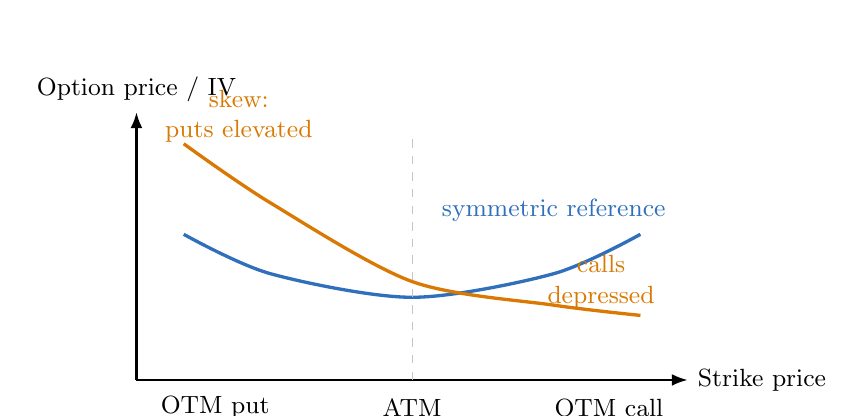
\begin{tikzpicture}[x=1cm,y=1cm,>=Latex]
  \draw[diagramAxis] (0,0) -- (7.0,0) node[right,font=\small]{Strike price};
  \draw[diagramAxis] (0,0) -- (0,3.4) node[above,font=\small]{Option price / IV};
  \draw[diagramBlue,very thick,smooth] plot coordinates {(0.6,1.85) (1.7,1.35) (3.5,1.05) (5.3,1.35) (6.4,1.85)};
  \draw[diagramOrange,very thick,smooth] plot coordinates {(0.6,3.0) (1.7,2.25) (3.5,1.25) (5.3,0.95) (6.4,0.82)};
  \draw[gray!45,dashed] (3.5,0) -- (3.5,3.1);
  \node[font=\small] at (1.0,-0.35) {OTM put};
  \node[font=\small] at (3.5,-0.35) {ATM};
  \node[font=\small] at (6.0,-0.35) {OTM call};
  \node[font=\small,diagramBlue] at (5.3,2.15) {symmetric reference};
  \node[font=\small,diagramOrange,align=center] at (1.3,3.35) {skew:\\puts elevated};
  \node[font=\small,diagramOrange,align=center] at (5.9,1.25) {calls\\depressed};
\end{tikzpicture}
\end{center}


\begin{itemize}[leftmargin=*]
    \item \textbf{Blue curve (symmetric):} Constant IV across all strikes. ATM put = ATM call price. OTM put equidistant from ATM = OTM call equidistant from ATM.
    \item \textbf{Orange curve (with skew):} The entire left side (puts) is elevated above the blue curve. The right side (calls) is depressed below it. This asymmetry \emph{is} the skew.
\end{itemize}

\textbf{Note:} The IV itself tells you the magnitude of the skew. Traders plot \textbf{IV against strike price} to measure and visualize skew — they don't plot price directly.

\subsubsection{The Real Skew Chart — SPY IV Viewer (Image 2)}

\textbf{Image 2} shows the actual volatility surface for SPY (S\&P 500 ETF) with:
\begin{itemize}[leftmargin=*]
    \item \textbf{X-axis:} Strike price (from 300 to 575)
    \item \textbf{Y-axis:} Implied Volatility (annualized \%, from ~10\% to ~37.5\%)
    \item \textbf{Multiple lines:} Sep (lightest), Oct, Nov, Dec, Jan 2022 (darkest blue) — each is one expiry date
    \item \textbf{Today (darker) vs. Yesterday (lighter):} Comparing changes over a month
\end{itemize}

\textbf{What you can observe:}
\begin{enumerate}[leftmargin=*]
    \item \textbf{Negative skew is visible:} Each curve slopes \textbf{downward from left to right} — IV is much higher for low strike prices (OTM puts) than for high strike prices (OTM calls). This is the classic SPY "smirk" (not a full symmetric smile).
    \item \textbf{At ATM (~446):} IV converges to a relatively low value. Below ATM, IV rises steeply; above ATM, IV rises only slightly.
    \item \textbf{OTM puts (left side, ~375–425 strikes):} IV is very elevated, reaching 27.5–37.5\% — significantly above ATM IV.
    \item \textbf{OTM calls (right side, ~475–550 strikes):} IV is only slightly elevated, in the 12.5–17.5\% range — near ATM levels.
    \item \textbf{All months' IVs were higher} on the observation day vs. a month ago — reflecting a general market anxiety increase even as the S\&P ground higher.
\end{enumerate}

\begin{quote}
The "smirk" (not a full "smile") is typical for equity indices: the left tail (crash risk) commands a much larger premium than the right tail (melt-up risk).
\end{quote}

\subsection{Term Structure of Volatility}

\subsubsection{What Is Term Structure?}

The \textbf{term structure of volatility} describes how implied volatility varies across \textbf{different expiration dates} for the same underlying (at, say, the ATM strike). It answers: "Is near-term IV higher or lower than longer-term IV?"

\subsubsection{Contango (Normal Condition)}

In normal, calm markets, the term structure is \textbf{upward-sloping} — called \textbf{contango}:


\begin{center}
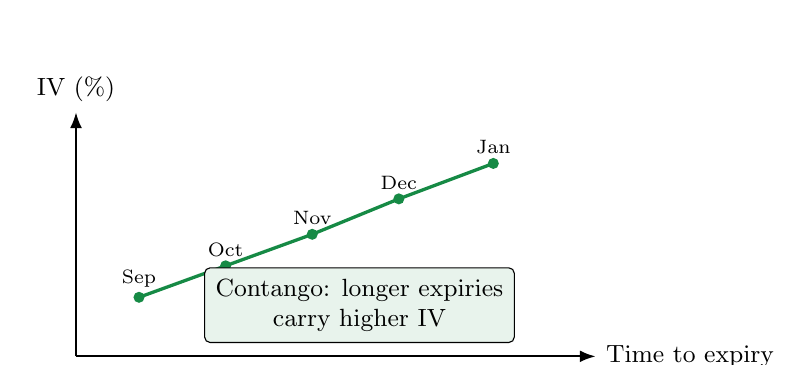
\begin{tikzpicture}[x=1cm,y=1cm,>=Latex]
  \draw[diagramAxis] (0,0) -- (6.6,0) node[right,font=\small]{Time to expiry};
  \draw[diagramAxis] (0,0) -- (0,3.1) node[above,font=\small]{IV (\%)};
  \draw[diagramGreen,very thick] (0.8,0.75) -- (1.9,1.15) -- (3.0,1.55) -- (4.1,2.0) -- (5.3,2.45);
  \foreach \x/\y/\m in {0.8/0.75/Sep,1.9/1.15/Oct,3.0/1.55/Nov,4.1/2.0/Dec,5.3/2.45/Jan}{
    \fill[diagramGreen] (\x,\y) circle (2pt); \node[font=\scriptsize,above] at (\x,\y) {\m};}
  \node[diagramBox,fill=diagramGreen!10] at (3.6,0.65) {Contango: longer expiries\\carry higher IV};
\end{tikzpicture}
\end{center}


\begin{itemize}[leftmargin=*]
    \item Short-term IV \(<\) Long-term IV
    \item Intuition: Over a longer period, there's more time for unknown events to cause volatility. Long-term uncertainty is priced higher.
    \item This is the \textbf{steady-state, non-fear condition}.
\end{itemize}

\subsubsection{Inverted Term Structure (Fear / Backwardation)}

When fear rises sharply (market selloffs, crises), the \textbf{short end of the term structure spikes} while the long end moves less:


\begin{center}
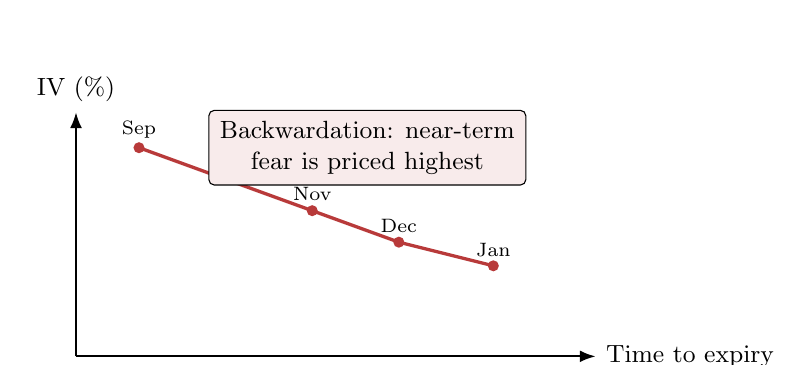
\begin{tikzpicture}[x=1cm,y=1cm,>=Latex]
  \draw[diagramAxis] (0,0) -- (6.6,0) node[right,font=\small]{Time to expiry};
  \draw[diagramAxis] (0,0) -- (0,3.1) node[above,font=\small]{IV (\%)};
  \draw[bearc,very thick] (0.8,2.65) -- (1.9,2.25) -- (3.0,1.85) -- (4.1,1.45) -- (5.3,1.15);
  \foreach \x/\y/\m in {0.8/2.65/Sep,1.9/2.25/Oct,3.0/1.85/Nov,4.1/1.45/Dec,5.3/1.15/Jan}{
    \fill[bearc] (\x,\y) circle (2pt); \node[font=\scriptsize,above] at (\x,\y) {\m};}
  \node[diagramBox,fill=bearc!10] at (3.7,2.65) {Backwardation: near-term\\fear is priced highest};
\end{tikzpicture}
\end{center}


\begin{itemize}[leftmargin=*]
    \item The curve \textbf{flattens or inverts}: near-term IV \(>\) long-term IV.
    \item Investors are pricing in immediate turmoil but expect things to calm down eventually.
\end{itemize}

\begin{quote}
\textbf{The VIX is essentially the front end of the term structure.} When the VIX spikes, the near-term portion of the curve moves dramatically while the far end moves much less.
\end{quote}

\subsubsection{At Different Strikes: Term Structure Can Reverse}

From \textbf{Image 2}, an important observation:

\begin{itemize}[leftmargin=*]
    \item \textbf{At ATM (~446 strike):} Moving from Oct \(\rightarrow\) Jan, IV increases (contango). This is expected.
    \item \textbf{At deep OTM puts (~400 strike):} The relationship \textbf{reverses} — near-term options (Oct) have \emph{higher} IV than longer-dated options (Jan) at that strike.
\end{itemize}

\textbf{Why?} OTM put options protect against near-term crashes. If a crash happens imminently, near-term OTM puts benefit most. This makes near-term OTM puts disproportionately demanded \(\rightarrow\) their IV is elevated above far-term equivalents.

\begin{quote}
\textbf{The full volatility "surface"} has skew across strikes AND term structure across expiries. Together they define a 3D landscape: strike \(\times\) expiry \(\times\) implied volatility.
\end{quote}

\subsection{How Skew Affects Option Spreads — The Key Counterintuitive Insight}

\subsubsection{Put Spreads Become CHEAPER with Elevated Skew}

This is the most important practical takeaway from skew, and it is \textbf{counterintuitive}:

\begin{quote}
\emph{When skew is elevated (puts have higher IV), put spreads paradoxically become }\emph{cheaper}\emph{ than call spreads — even though individual puts are more expensive.}
\end{quote}

\textbf{Here's why (refer to Image 3):}

Consider a put spread: \textbf{Buy an ATM put (P1), Sell an OTM put (P2)}.

With elevated skew, OTM puts have \textbf{disproportionately high IV} — their IV is even higher than the ATM put's IV. This means P2 (the put you \emph{sell}) is elevated more than P1 (the put you \emph{buy}).

\[
\text{Put Spread Cost} = \text{Price of P1} - \text{Price of P2}
\]

Since P2 is very expensive (high IV due to skew), you receive a large premium from selling it. This compresses the net cost of the spread:


\begin{center}
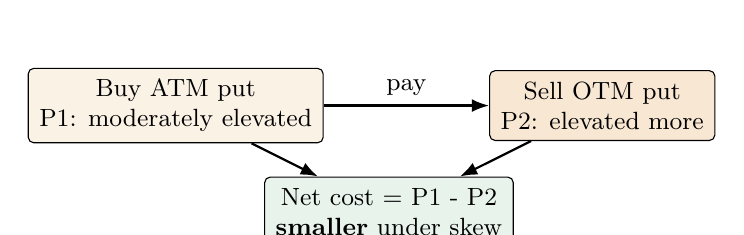
\begin{tikzpicture}[node distance=1.2cm,>=Latex]
  \node[diagramBox,fill=diagramOrange!10] (p1) {Buy ATM put\\P1: moderately elevated};
  \node[diagramBox,fill=diagramOrange!18,right=2.1cm of p1] (p2) {Sell OTM put\\P2: elevated more};
  \node[diagramBox,fill=diagramGreen!10] (net) at ($(p1)!0.5!(p2)+(0,-1.35)$) {Net cost = P1 - P2\\\textbf{smaller} under skew};
  \draw[diagramArrow] (p1) -- node[above,font=\small]{pay} (p2);
  \draw[diagramArrow] (p1) -- (net);
  \draw[diagramArrow] (p2) -- (net);
\end{tikzpicture}
\end{center}


For a call spread: \textbf{Buy an ATM call (C1), Sell an OTM call (C2)}.

With skew, calls are \textbf{depressed} in value. Specifically, C2 (the far OTM call you \emph{sell}) is even more depressed than C1.

\[
\text{Call Spread Cost} = \text{Price of C1} - \text{Price of C2}
\]

Since C2 brings in less premium (low IV), the net cost of the call spread is HIGHER than in the symmetric case.


\begin{center}
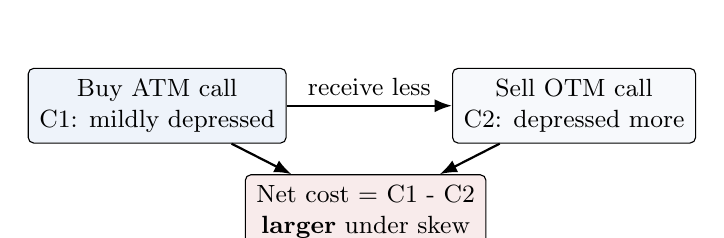
\begin{tikzpicture}[node distance=1.2cm,>=Latex]
  \node[diagramBox,fill=diagramBlue!8] (c1) {Buy ATM call\\C1: mildly depressed};
  \node[diagramBox,fill=diagramBlue!4,right=2.1cm of c1] (c2) {Sell OTM call\\C2: depressed more};
  \node[diagramBox,fill=bearc!10] (net) at ($(c1)!0.5!(c2)+(0,-1.35)$) {Net cost = C1 - C2\\\textbf{larger} under skew};
  \draw[diagramArrow] (c1) -- node[above,font=\small]{receive less} (c2);
  \draw[diagramArrow] (c1) -- (net);
  \draw[diagramArrow] (c2) -- (net);
\end{tikzpicture}
\end{center}


\subsubsection{Real Example: SPY December Spreads (ATM = \$446)}

From the video (Image 3, bottom-left annotations):

\begin{center}
\scriptsize
\setlength{\tabcolsep}{3pt}
\begin{tabular}{|L{3.0cm}|L{3.0cm}|L{3.0cm}|L{3.0cm}|}
\hline
\textbf{Spread} & \textbf{Structure} & \textbf{Width} & \textbf{Cost} \\
\hline
\textbf{Call spread} & Buy 446 call, Sell 476 call & 30 points up & \textbf{\$12.40} \\
\hline
\textbf{Put spread} & Buy 446 put, Sell 416 put & 30 points down & \textbf{\$7.56} \\
\hline
\end{tabular}
\end{center}

Both spreads are equal width (30 points), symmetric around ATM. Yet the put spread costs \textbf{\$4.84 less} than the call spread — entirely due to skew.

Maximum payoff for either spread: \textbf{30 points \(\times\) \$100 multiplier = \$3,000}.

\begin{center}
\scriptsize
\setlength{\tabcolsep}{3pt}
\begin{tabular}{|L{3.0cm}|L{3.0cm}|L{3.0cm}|L{3.0cm}|}
\hline
\textbf{Spread} & \textbf{Cost} & \textbf{Max Payoff} & \textbf{Risk:Reward} \\
\hline
Call spread & \$1,240 & \$3,000 & 1 : 2.4 \\
\hline
\textbf{Put spread} & \textbf{\$756} & \textbf{\$3,000} & \textbf{1 : 3.97} \\
\hline
\end{tabular}
\end{center}

\subsubsection{Real Example: SPY October Spreads (ATM = \$446)}

From the video (Image 3, bottom-right annotations):

\begin{center}
\scriptsize
\setlength{\tabcolsep}{3pt}
\begin{tabular}{|L{4.1cm}|L{4.1cm}|L{4.1cm}|}
\hline
\textbf{Spread} & \textbf{Key prices} & \textbf{Cost} \\
\hline
\textbf{Call spread} (446\(\rightarrow\)476) & 446 call = \$6.98; 476 call \(\approx\) \$0.05 (negligible) & \textbf{\$6.93} \\
\hline
\textbf{Put spread} (416\(\rightarrow\)446) & 446 put = \$8.25; 416 put = ? & \textbf{\$5.54} \\
\hline
\end{tabular}
\end{center}

Note: The 476 call (30 points OTM) costs virtually nothing (\$0.05) — the market assigns almost zero probability that SPY reaches 476 in a month. This further illustrates how depressed call IV is versus put IV in the skewed world.

\subsubsection{Risk Reversal — Zero-Cost Asymmetric Trade}

A \textbf{risk reversal} exploits skew by combining:
\begin{itemize}[leftmargin=*]
    \item \textbf{Sell an OTM put} (at elevated IV — receive a large premium)
    \item \textbf{Buy an OTM call} (at depressed IV — pay a small premium)
\end{itemize}

With sufficient skew, these can be structured to be \textbf{zero-cost} (the put premium received exactly funds the call purchase).

\textbf{December SPY example (from the video / Image 3 top-right):}

\[
\underbrace{\text{Sell 403 put}}_{\text{10\% below ATM}} + \underbrace{\text{Buy 460 call}}_{\text{3\% above ATM}} = \text{Zero net cost}
\]

\begin{itemize}[leftmargin=*]
    \item Downside risk: obligated to buy SPY at \$403 (10\% below current price of \$446) — but this is where the investor would want to buy anyway.
    \item Upside potential: unlimited participation above \$460.
    \item Net premium paid: \textbf{\$0}.
\end{itemize}

\begin{quote}
\textbf{In a symmetric world}, you would need symmetric strikes to achieve zero cost: e.g., sell the 416 put and buy the 476 call. Skew allows the put strike to be \textbf{much further OTM} while still generating enough premium to fund the call — creating highly asymmetric risk/reward.
\end{quote}

\subsection{VXX and Opposite Skew}

\subsubsection{What Is VXX?}

\textbf{VXX} (iPath S\&P 500 VIX Short-Term Futures ETN) is an ETF/ETN that attempts to track the VIX index by holding the \textbf{front two month VIX futures contracts}.

VXX tends to \textbf{rise when the market falls} (VIX spikes) and \textbf{fall when the market rises} (VIX falls). It is essentially a leveraged, short-duration bet on implied volatility.

\subsubsection{VXX Skew Is the Opposite of SPY}

Because VXX moves \emph{with} volatility and against stocks, investor behavior is reversed:
\begin{itemize}[leftmargin=*]
    \item When markets fall, VXX rises dramatically \(\rightarrow\) investors want \textbf{call} exposure on VXX
    \item Crash protection via VXX = buying calls (not puts)
\end{itemize}

\textbf{As a result:}
\begin{itemize}[leftmargin=*]
    \item VXX \textbf{calls} are in excess demand \(\rightarrow\) \textbf{call premiums elevated}
    \item VXX \textbf{puts} have less demand \(\rightarrow\) \textbf{put premiums depressed}
\end{itemize}


\begin{center}
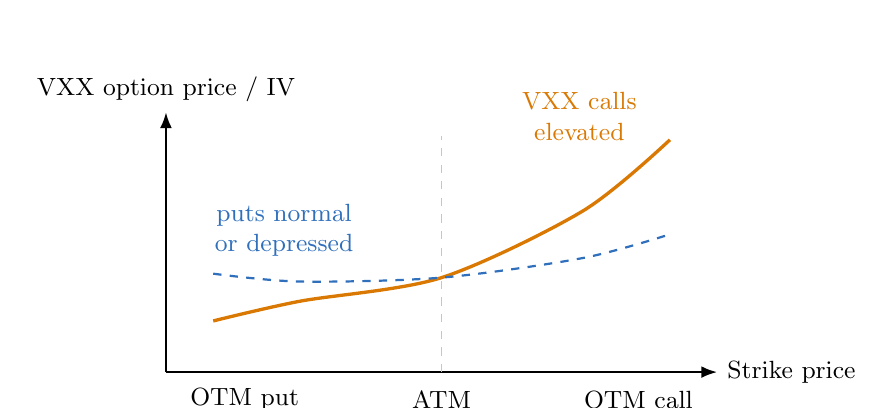
\begin{tikzpicture}[x=1cm,y=1cm,>=Latex]
  \draw[diagramAxis] (0,0) -- (7.0,0) node[right,font=\small]{Strike price};
  \draw[diagramAxis] (0,0) -- (0,3.3) node[above,font=\small]{VXX option price / IV};
  \draw[diagramOrange,very thick,smooth] plot coordinates {(0.6,0.65) (1.7,0.9) (3.5,1.2) (5.3,2.05) (6.4,2.95)};
  \draw[diagramBlue,thick,dashed,smooth] plot coordinates {(0.6,1.25) (1.7,1.15) (3.5,1.2) (5.3,1.45) (6.4,1.75)};
  \draw[gray!45,dashed] (3.5,0) -- (3.5,3.0);
  \node[font=\small] at (1.0,-0.35) {OTM put};
  \node[font=\small] at (3.5,-0.35) {ATM};
  \node[font=\small] at (6.0,-0.35) {OTM call};
  \node[font=\small,diagramOrange,align=center] at (5.25,3.25) {VXX calls\\elevated};
  \node[font=\small,diagramBlue,align=center] at (1.5,1.8) {puts normal\\or depressed};
\end{tikzpicture}
\end{center}


\begin{quote}
VXX has the \textbf{mirror image skew} of SPY. This means on VXX: \textbf{call spreads are cheap}, \textbf{put spreads are expensive} — the exact opposite of SPY.
\end{quote}

\subsubsection{Real VXX Trade Example (Image 4)}

From the video (ATM VXX = \$26, October expiry):

\textbf{VXX Symmetric Distribution (no skew context):}


\begin{center}
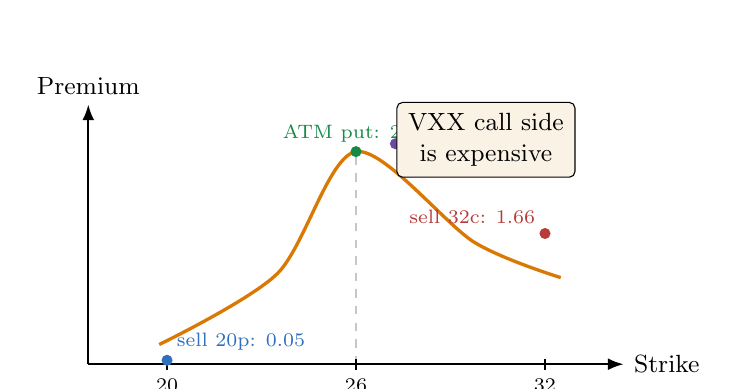
\begin{tikzpicture}[x=1cm,y=1cm,>=Latex]
  \draw[diagramAxis] (0,0) -- (6.8,0) node[right,font=\small]{Strike};
  \draw[diagramAxis] (0,0) -- (0,3.3) node[above,font=\small]{Premium};
  \draw[diagramOrange,very thick,smooth] plot coordinates {(0.9,0.25) (2.4,1.15) (3.4,2.7) (4.9,1.55) (6.0,1.1)};
  \draw[gray!45,dashed] (3.4,0) -- (3.4,2.75);
  \foreach \x/\lab in {1.0/20,3.4/26,5.8/32}{\draw (\x,0.07)--(\x,-0.07) node[below,font=\scriptsize]{\lab};}
  \fill[diagramBlue] (1.0,0.05) circle (2pt) node[above right,font=\scriptsize]{sell 20p: 0.05};
  \fill[diagramGreen] (3.4,2.70) circle (2pt) node[above,font=\scriptsize]{ATM put: 2.70};
  \fill[bearc] (5.8,1.66) circle (2pt) node[above left,font=\scriptsize]{sell 32c: 1.66};
  \fill[diagramPurple] (3.9,2.80) circle (2pt) node[right,font=\scriptsize]{buy call: 2.80};
  \node[diagramBox,fill=diagramOrange!10] at (5.05,2.85) {VXX call side\\is expensive};
\end{tikzpicture}
\end{center}


\begin{center}
\scriptsize
\setlength{\tabcolsep}{3pt}
\begin{tabular}{|L{3.0cm}|L{3.0cm}|L{3.0cm}|L{3.0cm}|}
\hline
\textbf{Spread} & \textbf{Structure} & \textbf{Cost} & \textbf{Max Payoff} \\
\hline
\textbf{Call spread} & Buy 26c @ \$2.80, Sell 32c @ \$1.66 & \textbf{\$1.14} & \$600 \\
\hline
\textbf{Put spread} & Buy 26p @ \$2.70, Sell 20p @ \$0.05 & \textbf{\$2.65} & \$600 \\
\hline
\end{tabular}
\end{center}

\[
\text{Call spread cost: \$1.14 for a \$600 payoff} \quad (1:5.26 \text{ risk:reward})
\]
\[
\text{Put spread cost: \$2.65 for a \$600 payoff} \quad (1:2.26 \text{ risk:reward})
\]

The call spread on VXX is \textbf{2.3\(\times\) cheaper} than the put spread for the same payoff — because VXX calls are cheap relative to puts (opposite of SPY).

\textbf{VXX trade thesis:} If you expect the market to sell off (e.g., VXX goes from \$26 to \$35, as it did in late July), the VXX call spread provides:
\begin{itemize}[leftmargin=*]
    \item \$1.14 cost \(\rightarrow\) \$600 potential payoff
    \item You can exit early at a profit even if VXX doesn't reach \$32 fully
    \item Cheap downside protection/speculative play for bearish traders who prefer VXX over SPY puts
\end{itemize}

\begin{quote}
\textbf{Practical insight:} If you're bearish on the market but nervous about SPY put margins or costs, the VXX call spread achieves the same economic exposure at potentially lower cost and with more intuitive position sizing.
\end{quote}

\subsection{Practical Summary: Skew-Informed Trading Decisions}

\begin{center}
\scriptsize
\setlength{\tabcolsep}{3pt}
\begin{tabular}{|L{3.0cm}|L{3.0cm}|L{3.0cm}|L{3.0cm}|}
\hline
\textbf{Instrument} & \textbf{Direction} & \textbf{Spread Type} & \textbf{Relative Cost (due to skew)} \\
\hline
\textbf{SPY} & Bearish & Put spread & \(\checkmark\) \textbf{Cheap} \\
\hline
\textbf{SPY} & Bullish & Call spread & \(\times\) Expensive \\
\hline
\textbf{SPY} & Neutral/Risk Reversal & Sell put + Buy call & \(\checkmark\) Zero or near-zero cost possible \\
\hline
\textbf{VXX} & Bullish (fear spike) & Call spread & \(\checkmark\) \textbf{Cheap} \\
\hline
\textbf{VXX} & Bearish (market rally) & Put spread & \(\times\) Expensive \\
\hline
\end{tabular}
\end{center}

\subsection{Volume vs. Liquidity}

\subsubsection{Definitions}

\textbf{Volume:}
The total number of shares, contracts, or units of a financial instrument traded during a given time period. Applies across stocks, bonds, options, futures, etc.

\textbf{Liquidity:}
The ease and speed with which an asset can be bought or sold in the market \textbf{at its current market price}, without causing a significant price impact.

\subsubsection{The Relationship}

Volume and liquidity are \textbf{positively correlated but not the same thing}:

\begin{itemize}[leftmargin=*]
    \item \textbf{High volume \(\rightarrow\) High liquidity} (generally): Active trading means market participants can enter/exit positions quickly near the current price. Bid-ask spreads are typically narrower.
    \item \textbf{Low volume \(\rightarrow\) Low liquidity}: The asset trades infrequently. Buying or selling large quantities may move the price significantly. Bid-ask spreads are wider.
\end{itemize}

\begin{quote}
Volume is an \textbf{indicator} of liquidity — not liquidity itself.
\end{quote}

\subsubsection{Why Liquidity Matters More to Investors}

\begin{center}
\scriptsize
\setlength{\tabcolsep}{3pt}
\begin{tabular}{|L{4.1cm}|L{4.1cm}|L{4.1cm}|}
\hline
\textbf{Factor} & \textbf{Volume} & \textbf{Liquidity} \\
\hline
What it measures & Quantity traded & Ease of trading at fair price \\
\hline
Ease of interpretation & Harder — requires context & More straightforward \\
\hline
Decision relevance & Secondary & Primary \\
\hline
\end{tabular}
\end{center}

Investors prefer analyzing liquidity because it \textbf{directly answers}: "Can I get in and out of this position quickly and at a fair price?" Volume requires more context to be meaningful (e.g., average volume, relative volume on news days, dark pool activity).

\begin{quote}
\textbf{For options specifically:} Liquidity in options is critical. Illiquid options have wide bid-ask spreads, meaning the cost of entering and exiting is significant even before any market movement — directly impacting profitability. Always check \textbf{open interest} and \textbf{bid-ask spread} before trading options.
\end{quote}

% -------------------- Introduction to Machine Learning for Finance --------------------
\chapter{Introduction to Machine Learning for Finance}

\section{Machine Learning and Stock Market}


\subsection{What Is Machine Learning?}
\index{Machine Learning}

\textbf{Machine Learning (ML)} is a subfield of artificial intelligence in which the core mechanism lies in a system's ability to:

\begin{enumerate}[leftmargin=*]
    \item \textbf{Understand the structure of data}
    \item \textbf{Align that data into models}
    \item \textbf{Use those models to make predictions or decisions}
\end{enumerate}

Unlike traditional programming, where a human explicitly writes all the rules, ML systems \textit{learn} those rules from data.

\subsubsection{Why ML in Finance?}

Finance is:
\begin{itemize}[leftmargin=*]
    \item \textbf{Highly nonlinear}: relationships between variables do not follow simple straight-line patterns.
    \item \textbf{High-dimensional}: prices are influenced by dozens or hundreds of factors simultaneously.
    \item \textbf{Non-stationary}: the data distribution changes over time through new market regimes, crises, and policy changes.
    \item \textbf{Sequential}: past prices and events influence future ones.
\end{itemize}

Traditional rule-based models struggle with these properties. ML, particularly neural networks, is designed to handle them.

\begin{quote}
\textbf{Historical shift:} Thirty years ago, investment required a human money manager. Today, robo-advisors and automated systems handle entire portfolios, often asking the user only for their risk profile. Machine learning has made this possible, and it is increasingly dominating institutional finance.
\end{quote}

\subsection{Types of Machine Learning}

\subsubsection{Supervised Learning}
\index{Supervised Learning}

In \textbf{supervised learning}, the algorithm is trained on a \textbf{labeled dataset}: data where the correct output, or label, is already known. The model learns a mapping from inputs to outputs by minimizing prediction error on the training data.

The rules or patterns are guided by human-labeled examples.

\textbf{Chess analogy:} IBM's \textbf{Deep Blue} (1997) was programmed using rules written by human chess players. The machine played in a human style, but faster and without fatigue. The knowledge structure was human-defined; the machine executed it better.

\textbf{Finance analogy:} A supervised model can be trained on historical stock data where observations are labeled as ``bull run'' or ``crash.'' The model then learns to recognize the features that precede each outcome.

\subsubsection{Unsupervised Learning}
\index{Unsupervised Learning}

In \textbf{unsupervised learning}, the algorithm receives \textbf{unlabeled data} and must find structure, patterns, or groupings on its own, without being told what the correct output is.

The algorithm discovers hidden patterns autonomously.

\textbf{Chess analogy:} Google's \textbf{AlphaZero} (2017) was given only the rules of chess and taught itself how to play through self-play. It needed just four hours of training to beat \textbf{Stockfish}, the world's best human-programmed chess engine. It discovered strategies humans had never conceived of.

\textbf{Finance analogy:} An unsupervised model can cluster stocks into groups based on return patterns without pre-labeling them as ``growth stocks'' or ``value stocks.'' The algorithm finds natural groupings in the data.

\begin{center}
\scriptsize
\setlength{\tabcolsep}{3pt}
\begin{tabular}{|L{3.0cm}|L{4.6cm}|L{4.6cm}|}
\hline
\textbf{Aspect} & \textbf{Supervised Learning} & \textbf{Unsupervised Learning} \\
\hline
Training data & Labeled & Unlabeled \\
\hline
Goal & Predict known categories or values & Discover hidden structure \\
\hline
Human role & Provides labels or rules & Provides only data \\
\hline
Example & Price prediction, classification & Clustering, dimensionality reduction \\
\hline
Chess analogy & Deep Blue & AlphaZero \\
\hline
\end{tabular}
\end{center}

\begin{quote}
In investment, the evolution mirrors chess: from systems with human-encoded strategies to systems that \textbf{create their own strategies} from raw market data.
\end{quote}

\subsection{Machine Learning in the Stock Market}

\subsubsection{The Old vs. New Approach}

\begin{center}
\scriptsize
\setlength{\tabcolsep}{3pt}
\begin{tabular}{|L{5.8cm}|L{5.8cm}|}
\hline
\textbf{Old Approach} & \textbf{New ML Approach} \\
\hline
Build a model based on a hypothesis, such as ``momentum predicts returns.'' & \textbf{Start with the data} and let the algorithm find patterns. \\
\hline
Test against historical data to validate or reject the hypothesis. & The model surfaces its own relationships and hypotheses. \\
\hline
Use human-defined features and rules. & The algorithm discovers features automatically. \\
\hline
\end{tabular}
\end{center}

\subsubsection{Quant Funds}
\index{Quantitative Funds}

A \textbf{quantitative (quant) fund} is an investment fund that selects securities using advanced quantitative analysis. Portfolio managers build customized mathematical and statistical models to determine optimal investments.

\textbf{Two broad types of quant funds:}
\begin{enumerate}[leftmargin=*]
    \item \textbf{Human-strategy quant funds:} Use ML to implement and optimize strategies that humans have designed. The model tests and refines human ideas at scale.
    \item \textbf{Self-strategy quant funds:} The algorithm itself generates the trading strategies by finding patterns in data, with no predetermined human hypothesis. The model decides what to look for.
\end{enumerate}

\begin{quote}
\textbf{Market share growth:} Quant funds now hold approximately 40\% of institutional trading shares, up from less than 20\% less than a decade ago. This trend is expected to accelerate as models become more powerful.
\end{quote}

\subsubsection{Correlation vs. Regression: An Important Distinction}
\index{Correlation}
\index{Regression}

Two concepts are often confused in market analysis.

\textbf{Correlation} measures the \textit{degree of association} between two or more independent variables that affect the market. It tells us that two variables move together, but not which one drives the other.

\begin{equation*}
    r = \frac{\sum (x_i - \bar{x})(y_i - \bar{y})}
    {\sqrt{\sum (x_i - \bar{x})^2 \cdot \sum (y_i - \bar{y})^2}} \in [-1, 1]
\end{equation*}

For example: ``Trading volume and price volatility are positively correlated.''

\textbf{Regression} quantifies the relationship between a \textbf{dependent variable}, such as stock price or return, and one or more \textbf{independent variables}, such as interest rates, earnings, or volume. It tells us how much a change in an independent variable predicts a change in the dependent variable.

For example: ``A 1\% increase in earnings growth predicts a 0.8\% increase in stock price.''

\begin{quote}
\textbf{Key distinction:} Correlation is symmetric and direction-agnostic. Regression has a clear dependent variable and enables prediction. Both are foundational to ML in finance.
\end{quote}

\subsection{Linear Regression for Price Prediction}
\index{Linear Regression}

\subsubsection{What It Does}

\textbf{Linear regression} estimates future price movements by fitting a \textbf{best-fit line}, or hyperplane in multiple dimensions, to historical market data. It models the relationship between one or more input features, called independent variables, and a continuous output such as a stock's future price or return.

\subsubsection{Mathematical Form}

\textbf{Simple linear regression} with one feature is written as:
\begin{equation*}
    \hat{y} = \beta_0 + \beta_1 x
\end{equation*}

\textbf{Multiple linear regression} with several features is written as:
\begin{equation*}
    \hat{y} = \beta_0 + \beta_1 x_1 + \beta_2 x_2 + \cdots + \beta_n x_n
\end{equation*}

where:
\begin{itemize}[leftmargin=*]
    \item \(\hat{y}\) is the predicted price or return.
    \item \(x_1, x_2, \ldots, x_n\) are input features such as trading volume, moving averages, or interest rates.
    \item \(\beta_0\) is the intercept, or baseline prediction when all features are zero.
    \item \(\beta_1, \ldots, \beta_n\) are coefficients that measure how much each feature contributes to the prediction.
\end{itemize}

\subsubsection{Fitting the Model: Ordinary Least Squares (OLS)}
\index{Ordinary Least Squares}

The coefficients are chosen to \textbf{minimize the sum of squared residuals}, where each residual is the difference between an actual value and its predicted value:
\begin{equation*}
    \min_{\beta} \sum_{i=1}^{N} \left( y_i - \hat{y}_i \right)^2
\end{equation*}

This finds the line, or hyperplane, that is closest to all data points in aggregate.

\subsubsection{Key Input Features in Finance}

\begin{center}
\scriptsize
\setlength{\tabcolsep}{3pt}
\begin{tabular}{|L{4.1cm}|L{8.1cm}|}
\hline
\textbf{Feature} & \textbf{What It Captures} \\
\hline
\textbf{Trading volume} & Market interest and conviction; high volume often confirms price moves. \\
\hline
\textbf{Moving averages} & Trend direction and mean-reversion signals, such as 50-day and 200-day moving averages. \\
\hline
\textbf{Macroeconomic variables} & GDP growth, inflation, interest rates, and other systemic drivers of asset prices. \\
\hline
\textbf{Earnings/fundamentals} & Company-specific value drivers. \\
\hline
\textbf{Past returns} & Lagged prices that may capture momentum or mean-reversion signals. \\
\hline
\end{tabular}
\end{center}

\subsubsection{Limitations of Linear Regression in Finance}

\begin{itemize}[leftmargin=*]
    \item Assumes a \textbf{linear relationship}, while financial markets are highly nonlinear.
    \item Is sensitive to \textbf{outliers}; market crashes can distort the fit dramatically.
    \item Does not capture \textbf{sequential dependencies} well, even though today's price often depends on yesterday's price.
    \item Cannot model \textbf{regime changes}; a bull-market model may fail in a bear market.
\end{itemize}

\subsection{Logistic Regression for Binary Classification}
\index{Logistic Regression}

\subsubsection{What It Does}

While linear regression predicts a \textit{continuous} value, such as price, \textbf{logistic regression} predicts a \textbf{binary outcome}. In finance, the most natural framing is:
\begin{equation*}
    \text{Output} =
    \begin{cases}
        1 & \text{if the stock price will rise} \\
        0 & \text{if the stock price will fall}
    \end{cases}
\end{equation*}

This turns price prediction into a \textbf{classification problem} and is one of the most common ML approaches for generating trading signals.

\subsubsection{Mathematical Form}

Logistic regression uses the \textbf{sigmoid}, or logistic, function to map any linear combination of features to a probability between 0 and 1:
\begin{equation*}
    P(\text{price rises}) = \sigma(z) = \frac{1}{1 + e^{-z}}
\end{equation*}
where:
\begin{equation*}
    z = \beta_0 + \beta_1 x_1 + \beta_2 x_2 + \cdots + \beta_n x_n
\end{equation*}

The sigmoid function \(\sigma(z)\) maps very negative inputs close to 0, very positive inputs close to 1, and \(z = 0\) to 0.5:

\begin{center}
\begin{tikzpicture}[x=1.0cm,y=3.0cm,>=Stealth]
    \draw[->] (-3.4,0) -- (3.6,0) node[right] {\(z\)};
    \draw[->] (-3.2,-0.05) -- (-3.2,1.1) node[above] {\(P(\text{rise})\)};
    \draw[dashed] (-3.2,0.5) -- (3.4,0.5);
    \node[left] at (-3.2,0) {0};
    \node[left] at (-3.2,0.5) {0.5};
    \node[left] at (-3.2,1) {1};
    \draw[domain=-3.1:3.1,smooth,variable=\x,blue,thick]
        plot ({\x},{1/(1+exp(-1.6*\x))});
    \node[below] at (0,0) {0};
    \node[below] at (-2.3,0) {\(z \ll 0\)};
    \node[below] at (2.3,0) {\(z \gg 0\)};
\end{tikzpicture}
\end{center}

\begin{itemize}[leftmargin=*]
    \item When \(z \rightarrow +\infty\), \(P \rightarrow 1\), giving a strong prediction of a rise.
    \item When \(z \rightarrow -\infty\), \(P \rightarrow 0\), giving a strong prediction of a fall.
    \item When \(z = 0\), \(P = 0.5\), giving an uncertain or neutral signal.
\end{itemize}

\subsubsection{Decision Rule}

\begin{equation*}
    \hat{y} =
    \begin{cases}
        1\ (\text{predict rise}) & \text{if } P(\text{rise}) > 0.5 \\
        0\ (\text{predict fall}) & \text{if } P(\text{rise}) \leq 0.5
    \end{cases}
\end{equation*}

The threshold of 0.5 can be adjusted based on the desired tradeoff between false positives, where the model predicts a rise but the price falls, and false negatives, where the model predicts a fall but the price rises.

\subsubsection{Same Input Features}

The same features used in linear regression apply here: trading volume, moving averages, macroeconomic indicators, sentiment scores, and other predictive variables. The difference is in the output: logistic regression produces a probability of moving up or down rather than a predicted price level.

\subsubsection{Linear vs. Logistic Regression}

\begin{center}
\scriptsize
\setlength{\tabcolsep}{3pt}
\begin{tabular}{|L{3.2cm}|L{4.5cm}|L{4.5cm}|}
\hline
\textbf{Aspect} & \textbf{Linear Regression} & \textbf{Logistic Regression} \\
\hline
Output type & Continuous price level or return & Binary up/down outcome \\
\hline
Output range & \(( -\infty, +\infty )\) & \((0, 1)\), interpreted as a probability \\
\hline
Loss function & Mean Squared Error (MSE) & Binary Cross-Entropy \\
\hline
Use case & Price or return forecasting & Trading signal generation, such as buy/sell decisions \\
\hline
\end{tabular}
\end{center}

\subsection{Deep Learning}
\index{Deep Learning}

\subsubsection{What Is Deep Learning?}

\textbf{Deep learning} is a subset of machine learning that uses \textbf{multi-layered neural networks} to learn hierarchical representations from raw data. It attempts to imitate how the human brain processes sensory information, such as light and sound, by progressively extracting higher-level features from lower-level inputs.

The key mechanism is non-linear processing of data, \textbf{layer by layer}. The output of each layer becomes the input to the next. Each successive layer learns increasingly abstract representations of the data.

\begin{center}
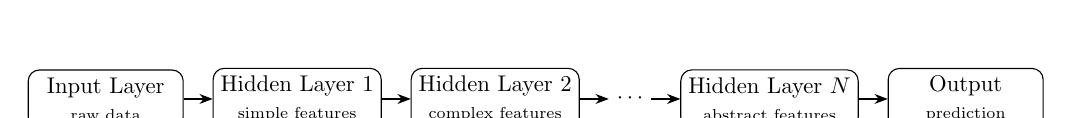
\begin{tikzpicture}[node distance=0.45cm,>=Stealth,scale=0.82,transform shape]
    \tikzstyle{layer}=[draw,rounded corners,align=center,minimum width=2.4cm,minimum height=0.8cm]
    \node[layer] (input) {Input Layer\\{\scriptsize raw data}};
    \node[layer,right=of input] (h1) {Hidden Layer 1\\{\scriptsize simple features}};
    \node[layer,right=of h1] (h2) {Hidden Layer 2\\{\scriptsize complex features}};
    \node[right=0.45cm of h2] (dots) {\(\cdots\)};
    \node[layer,right=0.45cm of dots] (hn) {Hidden Layer \(N\)\\{\scriptsize abstract features}};
    \node[layer,right=of hn] (output) {Output\\{\scriptsize prediction}};
    \draw[->] (input) -- (h1);
    \draw[->] (h1) -- (h2);
    \draw[->] (h2) -- (dots);
    \draw[->] (dots) -- (hn);
    \draw[->] (hn) -- (output);
\end{tikzpicture}
\end{center}

As the number of layers increases, the network's ability to learn complex, nonlinear relationships grows, compounding the learning rate and reducing the gradient of anomalies.

\subsubsection{Why Deep Learning Is Particularly Powerful for Finance}

Deep learning can \textbf{absorb massive amounts of historical market data}, including:
\begin{itemize}[leftmargin=*]
    \item Past price series across bull and bear markets.
    \item Historical crashes and crises, such as the 2008 crisis, the 2020 COVID crash, and the dot-com bust.
    \item Macroeconomic regime changes.
    \item Cross-asset correlations.
\end{itemize}

It then aggregates this data into successive categories of variables, which are interpreted in the context of an algorithmic model, without requiring a human to specify which variables matter.

\begin{quote}
\textbf{Key advantage:} Deep learning has historically beaten humans in cognitive tasks requiring financial analysis and decision-making, particularly because it can identify patterns that are \textbf{imperceptible to human analysis}.
\end{quote}

\subsubsection{The Risk}

The concern is that algorithms may converge on patterns that \textit{appear} predictive but do not reflect any real economic mechanism. These are \textbf{spurious correlations} in high-dimensional data. Human oversight remains important to validate that the discovered patterns are economically meaningful and not artifacts of overfitting.

\subsection{Neural Network Workflow for Stock Market Analysis}
\index{Neural Networks}

A neural network-based stock market model follows five stages.

\subsubsection{Stage 1: Data Acquisition}

Collect raw financial data:
\begin{itemize}[leftmargin=*]
    \item Historical price and volume data: open, high, low, close, and volume (OHLCV).
    \item Macroeconomic indicators, such as GDP, inflation, interest rates, and unemployment.
    \item Corporate fundamentals, such as earnings, revenue, and debt levels.
    \item Alternative data, such as news sentiment, social media, and satellite data.
    \item Options market data, such as implied volatility and put/call ratios.
\end{itemize}

\subsubsection{Stage 2: Data Preprocessing}

Raw financial data is messy. This stage involves:
\begin{itemize}[leftmargin=*]
    \item \textbf{Cleaning:} Removing outliers, handling missing values, and correcting data errors.
    \item \textbf{Normalization/Standardization:} Scaling features to comparable ranges so no single variable dominates.
    \item \textbf{Feature engineering:} Creating informative derived features such as moving averages, RSI, and Bollinger Bands.
    \item \textbf{Train/validation/test split:} Dividing data temporally by training on past data, validating during model development, and testing on unseen future data. The split must be time-aware to avoid \textbf{look-ahead bias}.
\end{itemize}

\subsubsection{Stage 3: Development and Implementation of a Model}

Design and build the neural network architecture. Key choices include:
\begin{itemize}[leftmargin=*]
    \item Type of network: MLP, RNN, LSTM, CNN, or Transformer.
    \item Number of layers and neurons.
    \item Activation functions.
    \item Optimizer and learning rate.
    \item Loss function.
\end{itemize}

\subsubsection{Stage 4: Backtest the Model}

Evaluate the model's performance on \textbf{historical data it has never seen during training}, usually the test set. Key metrics include:
\begin{itemize}[leftmargin=*]
    \item Prediction accuracy for classification or RMSE for regression.
    \item Sharpe ratio of the resulting strategy.
    \item Maximum drawdown.
    \item Hit rate, or the percentage of correct directional calls.
\end{itemize}

\begin{quote}
\textbf{Warning: Overfitting.} A model that memorizes the training data rather than learning generalizable patterns may backtest beautifully but fail in live trading. Proper validation, cross-validation, and regularization are critical.
\end{quote}

\subsubsection{Stage 5: Optimization}

Refine the model iteratively:
\begin{itemize}[leftmargin=*]
    \item \textbf{Hyperparameter tuning:} Adjust learning rate, layer sizes, and dropout rates.
    \item \textbf{Feature selection:} Remove irrelevant or noisy inputs.
    \item \textbf{Ensemble methods:} Combine predictions from multiple models.
    \item \textbf{Walk-forward optimization:} Continuously retrain as new market data arrives to prevent model staleness.
\end{itemize}

\subsection{Types of Neural Networks Used in Finance}

\subsubsection{Multilayer Perceptron (MLP)}
\index{Multilayer Perceptron}

The simplest and most common neural network architecture is the \textbf{multilayer perceptron (MLP)}.

\begin{center}
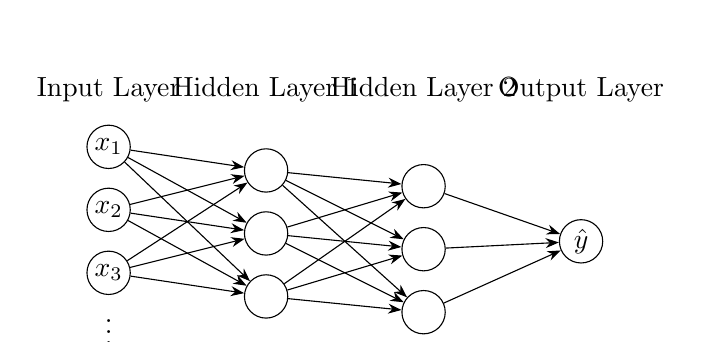
\begin{tikzpicture}[node distance=0.9cm,>=Stealth]
    \tikzstyle{node}=[circle,draw,minimum size=0.55cm,inner sep=0pt]
    \node[node] (x1) at (0,1.2) {\(x_1\)};
    \node[node] (x2) at (0,0.4) {\(x_2\)};
    \node[node] (x3) at (0,-0.4) {\(x_3\)};
    \node at (0,-1.05) {\(\vdots\)};
    \node[node] (h11) at (2,0.9) {};
    \node[node] (h12) at (2,0.1) {};
    \node[node] (h13) at (2,-0.7) {};
    \node[node] (h21) at (4,0.7) {};
    \node[node] (h22) at (4,-0.1) {};
    \node[node] (h23) at (4,-0.9) {};
    \node[node] (out) at (6,0) {\(\hat{y}\)};
    \foreach \from in {x1,x2,x3} {
        \foreach \to in {h11,h12,h13} {
            \draw[->,thin] (\from) -- (\to);
        }
    }
    \foreach \from in {h11,h12,h13} {
        \foreach \to in {h21,h22,h23} {
            \draw[->,thin] (\from) -- (\to);
        }
    }
    \foreach \from in {h21,h22,h23} {
        \draw[->,thin] (\from) -- (out);
    }
    \node[above] at (0,1.65) {Input Layer};
    \node[above] at (2,1.65) {Hidden Layer 1};
    \node[above] at (4,1.65) {Hidden Layer 2};
    \node[above] at (6,1.65) {Output Layer};
\end{tikzpicture}
\end{center}

\begin{itemize}[leftmargin=*]
    \item \textbf{Input:} Simple numerical features such as price, volume, and indicators.
    \item \textbf{Weights \(w_i\):} Learned importance of each input feature.
    \item \textbf{Hidden layers:} Non-linear transformations that capture complex relationships.
    \item \textbf{Output:} Predicted price or probability for classification.
\end{itemize}

\textbf{Limitation for sequential data:} MLPs process each input independently. They have no built-in mechanism to account for the \textit{sequence} or temporal order of observations. This is a significant drawback for time-series data like stock prices.

\subsubsection{Recurrent Neural Networks (RNN) and LSTM}
\index{Recurrent Neural Networks}
\index{Long Short-Term Memory}

\textbf{Recurrent Neural Networks (RNNs)} address the sequential limitation of MLPs by maintaining a \textbf{hidden state} that carries information from previous time steps:

\begin{center}
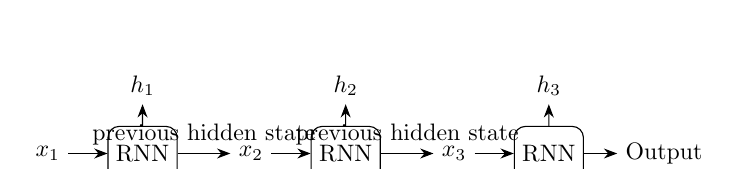
\begin{tikzpicture}[node distance=1.0cm,>=Stealth,scale=0.86,transform shape]
    \tikzstyle{rnn}=[draw,rounded corners,minimum width=1.0cm,minimum height=0.8cm]
    \node (x1) at (0,0) {\(x_1\)};
    \node[rnn] (r1) at (1.4,0) {RNN};
    \node (h1) at (1.4,1.0) {\(h_1\)};
    \node (x2) at (3.0,0) {\(x_2\)};
    \node[rnn] (r2) at (4.4,0) {RNN};
    \node (h2) at (4.4,1.0) {\(h_2\)};
    \node (x3) at (6.0,0) {\(x_3\)};
    \node[rnn] (r3) at (7.4,0) {RNN};
    \node (h3) at (7.4,1.0) {\(h_3\)};
    \node (out) at (9.1,0) {Output};
    \draw[->] (x1) -- (r1);
    \draw[->] (r1) -- (x2) node[midway,above] {previous hidden state};
    \draw[->] (x2) -- (r2);
    \draw[->] (r2) -- (x3) node[midway,above] {previous hidden state};
    \draw[->] (x3) -- (r3);
    \draw[->] (r3) -- (out);
    \draw[->] (r1) -- (h1);
    \draw[->] (r2) -- (h2);
    \draw[->] (r3) -- (h3);
\end{tikzpicture}
\end{center}

Each time step receives both the \textbf{new input} and the \textbf{previous hidden state}, allowing the network to ``remember'' earlier observations when making current predictions.

\textbf{Long Short-Term Memory (LSTM)} is a specialized, more powerful form of RNN designed to overcome the \textbf{vanishing gradient problem}, where the network forgets information from many steps back. LSTMs contain:
\begin{itemize}[leftmargin=*]
    \item A \textbf{cell state}, or long-term memory.
    \item An \textbf{input gate}, which controls what new information to store.
    \item A \textbf{forget gate}, which controls what old information to discard.
    \item An \textbf{output gate}, which controls what information to output.
\end{itemize}

\textbf{Why LSTMs are ideal for stock market prediction:}
\begin{itemize}[leftmargin=*]
    \item Stock prices are \textbf{sequential}; yesterday's price is relevant to today's.
    \item LSTMs can model \textbf{long-range dependencies}, detecting patterns across days, weeks, or months of data.
    \item They can capture the interplay between current price data and historical price data.
    \item As the number of LSTM layers increases, the ability to model complex nonlinear temporal relationships grows.
    \item They help \textbf{decrease the gradient of anomalies}, smoothing out single-day outliers that could otherwise distort predictions.
\end{itemize}

\subsubsection{Implementation: Keras}
\index{Keras}

\textbf{Keras} is a standard open-source Python library for building neural networks for this type of financial modeling. Key advantages include:
\begin{itemize}[leftmargin=*]
    \item Builds networks by \textbf{successively adding layers}, rather than defining the entire architecture at once.
    \item Supports MLP, RNN, LSTM, and more complex architectures.
    \item Is tightly integrated with TensorFlow.
    \item Is well-suited to adapting models quickly when \textbf{market conditions shift}; the market can ``flip'' rapidly, and Keras's modular layer-based approach allows fast iteration.
\end{itemize}

\begin{Verbatim}[fontsize=\small,breaklines=true]
# Simplified example of a Keras LSTM for stock prediction
from keras.models import Sequential
from keras.layers import LSTM, Dense, Dropout

model = Sequential()
model.add(LSTM(units=64, return_sequences=True,
               input_shape=(time_steps, features)))
model.add(Dropout(0.2))
model.add(LSTM(units=32))
model.add(Dense(units=1))  # Output: predicted price or probability
model.compile(optimizer='adam', loss='mean_squared_error')
\end{Verbatim}

\subsection{Risks, Concerns, and Limitations}

\subsubsection{Flash Crises}

One major risk of algorithm-dominated markets is the potential for \textbf{``flash crises''}: sudden, severe market dislocations caused by algorithms acting in concert without human override. For example, in 2014, bond prices rallied sharply by more than 5\% in minutes, a move that no fundamental news justified and that was driven by high-frequency algorithmic trading.

\textbf{Why algorithms exacerbate volatility:}
\begin{itemize}[leftmargin=*]
    \item They react to the same signals simultaneously, creating herding behavior.
    \item High-volume automated traders provide liquidity \textit{in normal times} but may withdraw simultaneously during stress, creating a sudden liquidity vacuum.
\end{itemize}

\subsubsection{Emotion-Free Trading: An Advantage}

A significant benefit of algorithmic trading is the \textbf{absence of human emotion}:
\begin{itemize}[leftmargin=*]
    \item No panic selling during market drops.
    \item No greed-driven overconcentration in ``hot'' stocks.
    \item No anchoring, confirmation bias, or loss aversion.
    \item Consistent, rule-based execution around the clock.
\end{itemize}

The argument is that algorithms applied with discipline may produce better risk-adjusted outcomes than human fund managers subject to behavioral biases.

\subsubsection{The Edge Problem: Normalization Over Time}

If a fund develops a sufficiently powerful ML model, it gains an \textbf{imperceptible informational edge} over competitors. However, the historical pattern suggests:
\begin{itemize}[leftmargin=*]
    \item Alpha discovered by quant funds gets competed away as more firms adopt similar models.
    \item The edge eventually \textbf{normalizes}; once everyone has the same technology, it no longer confers an advantage.
    \item The arms race then moves to data quality, compute power, and model architecture improvements.
\end{itemize}

\subsubsection{Interpretability: The Black Box Problem}

Deep learning models, despite their predictive power, are often \textbf{opaque}: it is difficult to explain \textit{why} a model made a particular prediction. In finance, this is problematic because:
\begin{itemize}[leftmargin=*]
    \item Regulatory requirements may demand explainability.
    \item Risk management requires understanding \textit{what} the model has learned.
    \item Models may exploit spurious correlations that break down in new market regimes.
\end{itemize}

\begin{quote}
``Sometimes in the indexes of the stock market, human leverage or control is required to understand the complexities of what actually drives the market, rather than arbitrary variables contrived by computers.'' This is the core argument for keeping humans in the loop.
\end{quote}


\section{Regression}

\subsection{What is Regression Analysis?}


\subsubsection{Definition}


Regression analysis is a statistical method that allows you to \textbf{infer or predict the value of one variable based on one or more other variables}. It models the relationship between a dependent variable (what you want to predict) and one or more independent variables (what you use to predict).

\textbf{Two core goals:}

\begin{center}
\small
\renewcommand{\arraystretch}{1.15}
\begin{tabular}{|L{0.22\textwidth}|L{0.30\textwidth}|L{0.36\textwidth}|}
\hline
    Goal & Description & Example \\
\hline
    \textbf{Measure Influence} & Determine whether and how much certain variables affect another & Does education level influence salary? \\
\hline
    \textbf{Predict} & Use known variable values to forecast an unknown value & Predict hospital stay length from patient age \\
\hline
\end{tabular}
\end{center}
\normalsize


\subsubsection{Terminology}


\begin{center}
\small
\renewcommand{\arraystretch}{1.15}
\begin{tabular}{|L{0.22\textwidth}|L{0.30\textwidth}|L{0.36\textwidth}|}
\hline
    Term & Alternative Name & Meaning \\
\hline
    \textbf{Dependent Variable} & Criterion, Response Variable, Y & The variable you want to predict/explain \\
\hline
    \textbf{Independent Variable} & Predictor, Explanatory Variable, X & The variable(s) used for prediction \\
\hline
\end{tabular}
\end{center}
\normalsize


\textbf{Examples of dependent variables:} Salary, body height, shoe size, electricity consumption, hospital stay length, probability of burnout.

\medskip


\subsection{Types of Regression}



\begin{center}
\resizebox{0.92\textwidth}{!}{%
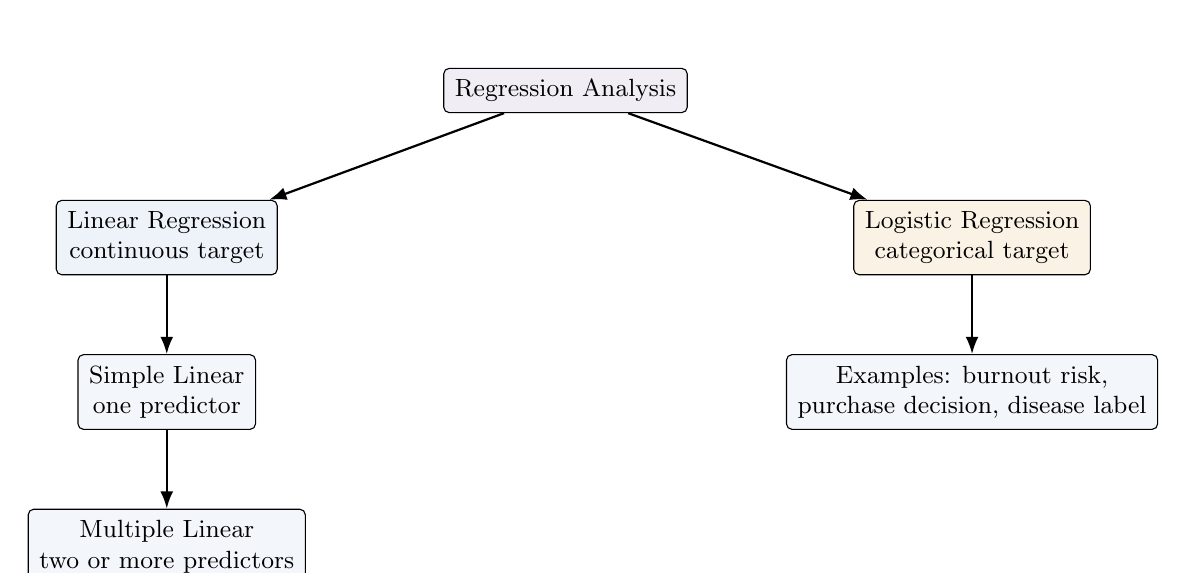
\begin{tikzpicture}[node distance=1.0cm and 1.5cm,>=Latex]
  \node[diagramBox,fill=diagramPurple!10] (root) {Regression Analysis};
  \node[diagramBox,fill=diagramBlue!8,below left=1.1cm and 2.1cm of root] (linear) {Linear Regression\\continuous target};
  \node[diagramBox,fill=diagramOrange!10,below right=1.1cm and 2.1cm of root] (logistic) {Logistic Regression\\categorical target};
  \node[diagramBox,below=1.0cm of linear] (simple) {Simple Linear\\one predictor};
  \node[diagramBox,below=1.0cm of simple] (multiple) {Multiple Linear\\two or more predictors};
  \node[diagramBox,below=1.0cm of logistic] (binary) {Examples: burnout risk,\\purchase decision, disease label};
  \draw[diagramArrow] (root) -- (linear);
  \draw[diagramArrow] (root) -- (logistic);
  \draw[diagramArrow] (linear) -- (simple);
  \draw[diagramArrow] (simple) -- (multiple);
  \draw[diagramArrow] (logistic) -- (binary);
\end{tikzpicture}%
}
\end{center}



\textbf{Key distinction:}
\begin{itemize}[leftmargin=*]
    \item In \textbf{linear regression}, the dependent variable is metric (continuous, measurable): salary, height, consumption, stay duration.
    \item In \textbf{logistic regression}, the dependent variable is categorical (binary or ordered): Yes/No, sick/healthy, buy/don't buy.

\end{itemize}

\textbf{Note:} Independent variables can have any scale (nominal, ordinal, metric) in all regression types. If categorical independent variables have more than 2 categories, they must be converted to dummy variables.

\medskip


\subsection{Simple Linear Regression}


\subsubsection{The Core Idea: Predicting with One Variable}


\textbf{Problem setup (Tips for Service):}
A restaurant owner collects tip amounts for 6 meals: \$5, \$17, \$11, \$8, \$14, \$5.

\textbf{With only one variable (tip amount), the best prediction for any future tip is the mean:}

\[
\bar{Y} = \frac{5 + 17 + 11 + 8 + 14 + 5}{6} = \$10
\]


The mean is the best estimate when you have no other information. If you graph this, the best-fit line is a \textbf{flat horizontal line at \$10} --- a line with slope = 0.

\begin{quote}
\textbf{This is the baseline model.} Simple linear regression always compares its performance against this baseline --- the situation where the independent variable doesn't exist and we use only the mean of Y.
\end{quote}


\medskip


\subsubsection{Residuals and the Sum of Squared Errors (SSE)}


A \textbf{residual} (also called the \textbf{error}) is the difference between the actual observed value and the value predicted by the model:

\[
\text{Residual}_i = y_i - \hat{y}_i
\]


\textbf{Key properties of residuals:}
\begin{enumerate}[leftmargin=*]
    \item Residuals always \textbf{sum to zero} (they balance above and below the line).
    \item They measure \textbf{how far off} the model's predictions are.

\end{enumerate}

\textbf{Why square the residuals?}
\begin{itemize}[leftmargin=*]
    \item Makes all values positive (a deviation of -5 and +5 are equally "wrong").
    \item Emphasizes larger errors more than small ones (a deviation of 5 squares to 25; a deviation of 2 only squares to 4).

\end{itemize}

\textbf{Sum of Squared Errors (SSE):}

\[
\text{SSE} = \sum_{i=1}^{n} (y_i - \hat{y}_i)^2
\]


\textbf{Tip example --- calculating SSE with the baseline model (mean = \$10):}

\begin{center}
\scriptsize
\renewcommand{\arraystretch}{1.15}
\begin{tabular}{|L{0.07\textwidth}|L{0.14\textwidth}|L{0.23\textwidth}|L{0.12\textwidth}|L{0.13\textwidth}|}
\hline
    Meal & Actual Tip (\(y_i\)) & Predicted (\(\hat{y}_i = \bar{Y}\)) & Residual & Residual\textsuperscript{2} \\
\hline
    1 & \$5 & \$10 & -5 & 25 \\
\hline
    2 & \$17 & \$10 & +7 & 49 \\
\hline
    3 & \$11 & \$10 & +1 & 1 \\
\hline
    4 & \$8 & \$10 & -2 & 4 \\
\hline
    5 & \$14 & \$10 & +4 & 16 \\
\hline
    6 & \$5 & \$10 & -5 & 25 \\
\hline
     &  &  & \textbf{Sum = 0} & \textbf{SSE = 120} \\
\hline
\end{tabular}
\end{center}
\normalsize


\begin{quote}
\textbf{The goal of simple linear regression is to find a line that minimizes the SSE} --- specifically, to reduce it below the baseline SSE of 120 by introducing the independent variable (meal amount).
\end{quote}


\medskip


\subsubsection{The Algebra of Regression Lines}


Regression lines follow the \textbf{slope-intercept form}:

\[
y = mx + b
\]


Or in the regression context for a \textbf{population model:}

\[
y = \beta_0 + \beta_1 x + \varepsilon
\]


And for \textbf{sample estimation:}

\[
\hat{y} = b_0 + b_1 x
\]


\begin{center}
\small
\renewcommand{\arraystretch}{1.15}
\begin{tabular}{|L{0.28\textwidth}|L{0.60\textwidth}|}
\hline
    Symbol & Meaning \\
\hline
    \(\beta_0\) (population) / \(b_0\) (sample) & \textbf{Y-intercept} --- the value of Y when X = 0 \\
\hline
    \(\beta_1\) (population) / \(b_1\) (sample) & \textbf{Slope} --- how much Y changes for a 1-unit increase in X \\
\hline
    \(\varepsilon\) & \textbf{Error term} --- unexplained variation (absent in sample equation as it's assumed = 0 in expectation) \\
\hline
    \(\hat{y}\) ("y-hat") & \textbf{Predicted value} of Y --- the point estimator \\
\hline
\end{tabular}
\end{center}
\normalsize


\textbf{Three general shapes based on slope:}


\begin{center}
\resizebox{\textwidth}{!}{%
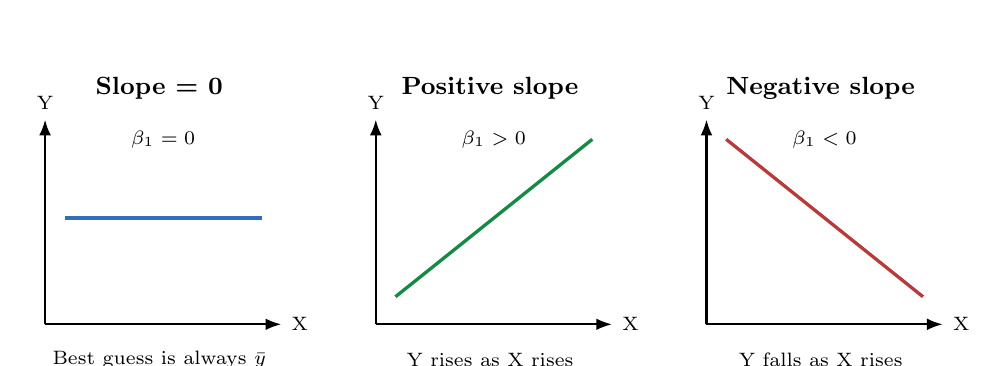
\begin{tikzpicture}[x=1cm,y=1cm,>=Latex]
  \foreach \x/\title/\desc in {0/{Slope = 0}/{Best guess is always \(\bar y\)},4.2/{Positive slope}/{Y rises as X rises},8.4/{Negative slope}/{Y falls as X rises}}{
    \draw[diagramAxis] (\x,0) -- +(3.0,0) node[right,font=\scriptsize]{X};
    \draw[diagramAxis] (\x,0) -- +(0,2.6) node[above,font=\scriptsize]{Y};
    \node[font=\small\bfseries] at (\x+1.45,3.0) {\title};
    \node[font=\scriptsize,align=center] at (\x+1.45,-0.45) {\desc};
  }
  \draw[diagramBlue,very thick] (0.25,1.35) -- (2.75,1.35);
  \draw[diagramGreen,very thick] (4.45,0.35) -- (6.95,2.35);
  \draw[bearc,very thick] (8.65,2.35) -- (11.15,0.35);
  \node[font=\scriptsize] at (1.5,2.35) {\(\beta_1=0\)};
  \node[font=\scriptsize] at (5.7,2.35) {\(\beta_1>0\)};
  \node[font=\scriptsize] at (9.9,2.35) {\(\beta_1<0\)};
\end{tikzpicture}%
}
\end{center}



\begin{quote}
\textbf{If the regression line is flat (slope = 0)}, the independent variable adds nothing --- the model is no better than using the mean alone. The goal of regression is to find a slope that meaningfully differs from zero.
\end{quote}


\medskip


\subsubsection{The Regression Line: Coefficients and Their Calculation}


For simple linear regression, the slope and intercept can be calculated:

\[
b_1 = r \times \frac{s_y}{s_x}
\]


\[
b_0 = \bar{y} - b_1 \bar{x}
\]


Where:
\begin{itemize}[leftmargin=*]
    \item \(r\) = Pearson correlation coefficient between X and Y
    \item \(s_y\) = standard deviation of Y
    \item \(s_x\) = standard deviation of X
    \item \(\bar{y}\) = mean of Y
    \item \(\bar{x}\) = mean of X

\end{itemize}

\begin{quote}
In practice, a statistics software package (Python, R, SPSS, Excel) calculates these using the \textbf{method of least squares} --- an algorithm that finds the unique line minimizing the SSE. This optimal solution is derived from calculus (setting derivatives of SSE to zero), but you generally rely on software for computation.
\end{quote}


\textbf{The regression line always passes through the point \((\bar{x}, \bar{y})\).}

\medskip


\subsubsection{Worked Example: Hospital Stay Prediction}


\textbf{Setup:}
\begin{itemize}[leftmargin=*]
    \item Dependent variable (Y): Length of hospital stay after surgery (days)
    \item Independent variable (X): Patient age (years)
    \item Fitted model: \(\hat{y} = 1.22 + 0.14x\)

\end{itemize}

\textbf{Interpretation:}
\begin{itemize}[leftmargin=*]
    \item \(b_0 = 1.22\): If a patient were 0 years old (theoretical baseline), the model predicts 1.22 days of stay.
    \item \(b_1 = 0.14\): Each additional year of age adds 0.14 days to the predicted stay.

\end{itemize}

\textbf{Prediction for a 33-year-old patient:}

\[
\hat{y} = 1.22 + 0.14 \times 33 = 1.22 + 4.62 = 5.82 \text{ days}
\]


\textbf{Error (residual):} If the patient actually stayed 7 days:
\[
\varepsilon = 7 - 5.82 = 1.18 \text{ days}
\]


\medskip


\subsubsection{Interpreting Regression Results}


A regression output typically shows:

\textbf{1. Model Summary}

\begin{center}
\small
\renewcommand{\arraystretch}{1.15}
\begin{tabular}{|L{0.22\textwidth}|L{0.30\textwidth}|L{0.36\textwidth}|}
\hline
    Metric & Symbol & Meaning \\
\hline
    \textbf{Multiple Correlation Coefficient} & R & Correlation between actual Y and predicted \(\hat{y}\). Higher = better model. \\
\hline
    \textbf{Coefficient of Determination} & R\textsuperscript{2} & Proportion of variance in Y explained by the model. Ranges 0--1. R\textsuperscript{2} = 1 means perfect prediction. \\
\hline
    \textbf{Adjusted R\textsuperscript{2}} & Adj. R\textsuperscript{2} & R\textsuperscript{2} corrected for the number of predictors (prevents overfitting inflation). Use this for multiple regression. \\
\hline
    \textbf{Standard Error of Estimation} & SEE & Average deviation of predictions from actual values. Lower = more precise predictions. \\
\hline
\end{tabular}
\end{center}
\normalsize


\begin{quote}
\textbf{Example interpretation:} R\textsuperscript{2} = 0.49 means the predictors explain \textbf{49\% of the variance} in salary. The other 51\% is unexplained (random variation, missing variables, etc.).
\end{quote}


\textbf{2. F-Test (ANOVA Table)}

Tests the null hypothesis: \textit{All slope coefficients in the population are zero} (i.e., the model is no better than the baseline).

\[
H_0: \beta_1 = \beta_2 = \dots = \beta_k = 0
\]


\begin{itemize}[leftmargin=*]
    \item \textbf{p \(<\) 0.05:} Reject \(H_0\) --- the model is statistically significant overall.
    \item \textbf{p \(\geq\) 0.05:} Fail to reject \(H_0\) --- cannot conclude the model is useful.

\end{itemize}

\textbf{3. Individual Coefficient Table}

\begin{center}
\small
\renewcommand{\arraystretch}{1.15}
\begin{tabular}{|L{0.28\textwidth}|L{0.60\textwidth}|}
\hline
    Column & Meaning \\
\hline
    \textbf{B (Unstandardized)} & Raw coefficients to plug into the regression equation \\
\hline
    \textbf{Beta (Standardized)} & Coefficients scaled to standard deviations --- shows which predictor has the \textbf{largest relative effect} \\
\hline
    \textbf{Significance (p-value)} & Tests if each coefficient = 0 in the population. p \(<\) 0.05 \(\rightarrow\) coefficient is significant \\
\hline
\end{tabular}
\end{center}
\normalsize


\begin{quote}
\textbf{Example:} If Beta for Age = 0.45 and Beta for Weight = 0.12, age has a stronger influence on salary than weight in relative terms.
\end{quote}


\medskip




\subsubsection{Statistical Foundation of Simple Linear Regression}

The sample equation \(\hat{y}=b_0+b_1x\) is an estimate of a population relationship. A rigorous statistical model writes each observation as
\[
Y_i=\beta_0+\beta_1x_i+\varepsilon_i, \qquad i=1,2,\dots,n.
\]
Here \(x_i\) is treated as known or fixed by design, while \(Y_i\) is random because it contains the error term \(\varepsilon_i\). The key population assumptions are:
\begin{enumerate}[leftmargin=*]
    \item \textbf{Zero conditional mean:} \(E[\varepsilon_i\mid x_i]=0\). This says the regression line is centered correctly; no systematic information about \(Y\) remains in the error once \(x\) is known.
    \item \textbf{Constant variance:} \(\operatorname{Var}(\varepsilon_i\mid x_i)=\sigma^2\). This is homoscedasticity.
    \item \textbf{No error correlation:} \(\operatorname{Cov}(\varepsilon_i,\varepsilon_j)=0\) for \(i\neq j\). This is especially important in time series.
    \item \textbf{Optional normality for exact small-sample inference:} \(\varepsilon_i\sim N(0,\sigma^2)\). Normality is not required for the OLS line to be unbiased, but it gives exact \(t\)-tests and \(F\)-tests in small samples.
\end{enumerate}

\begin{quote}
\textbf{Interpretation:} Simple linear regression does not claim that every point lies on one deterministic line. It claims that the \textit{conditional mean} of \(Y\) is linear in \(X\):
\[
E[Y\mid X=x]=\beta_0+\beta_1x.
\]
The error term captures all influences on \(Y\) that are not represented by \(x\).
\end{quote}

\subsubsection{Least-Squares Derivation from First Principles}

Ordinary least squares chooses \(b_0\) and \(b_1\) to minimize the residual sum of squares:
\[
S(b_0,b_1)=\sum_{i=1}^{n}(y_i-b_0-b_1x_i)^2.
\]
The first-order conditions are obtained by differentiating with respect to both unknown coefficients:
\begin{align*}
\frac{\partial S}{\partial b_0} &=-2\sum_{i=1}^{n}(y_i-b_0-b_1x_i)=0,\\
\frac{\partial S}{\partial b_1} &=-2\sum_{i=1}^{n}x_i(y_i-b_0-b_1x_i)=0.
\end{align*}
These are called the \textbf{normal equations}. They imply two important orthogonality conditions:
\[
\sum_{i=1}^{n}e_i=0, \qquad \sum_{i=1}^{n}x_ie_i=0,
\]
where \(e_i=y_i-\hat{y}_i\). Thus residuals sum to zero and are uncorrelated with the regressor used to fit the line.

Solving the normal equations gives the closed-form OLS estimates:
\begin{align*}
b_1 &= \frac{\sum_{i=1}^{n}(x_i-\bar{x})(y_i-\bar{y})}{\sum_{i=1}^{n}(x_i-\bar{x})^2}=\frac{S_{xy}}{S_{xx}},\\
b_0 &= \bar{y}-b_1\bar{x}.
\end{align*}
This derivation also proves why the fitted line must pass through \((\bar{x},\bar{y})\): substituting \(x=\bar{x}\) gives \(\hat{y}=b_0+b_1\bar{x}=\bar{y}\).

\paragraph{Geometric intuition.}
Think of the observed vector \(y\) as a point in \(n\)-dimensional space. The fitted values \(\hat{y}\) are the orthogonal projection of \(y\) onto the two-dimensional plane spanned by a constant column and the regressor column \(x\). The residual vector \(e=y-\hat{y}\) is perpendicular to that plane:
\[
\mathbf{1}'e=0, \qquad x'e=0.
\]
This is why OLS is often described as finding the ``closest'' line to the data in Euclidean distance.


\begin{center}
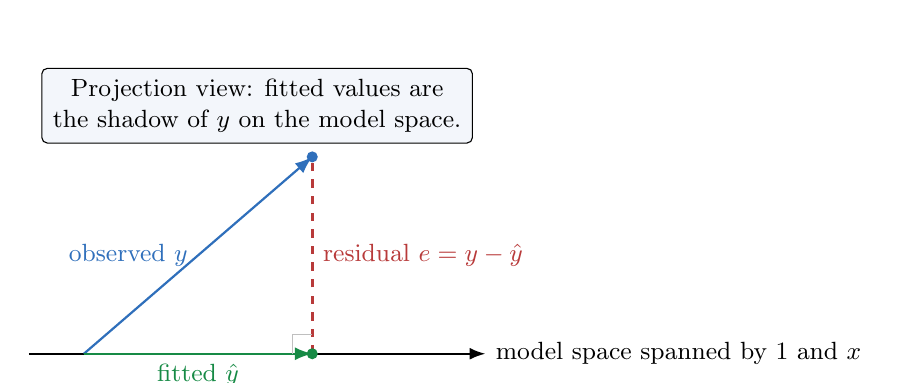
\begin{tikzpicture}[x=1cm,y=1cm,>=Latex]
  \draw[diagramAxis] (0,0) -- (5.8,0) node[right,font=\small]{model space spanned by \(1\) and \(x\)};
  \coordinate (origin) at (0.7,0);
  \coordinate (yhat) at (3.6,0);
  \coordinate (y) at (3.6,2.5);
  \draw[diagramArrow,diagramBlue] (origin) -- (y) node[midway,left,font=\small]{observed \(y\)};
  \draw[diagramArrow,diagramGreen] (origin) -- (yhat) node[midway,below,font=\small]{fitted \(\hat y\)};
  \draw[bearc,very thick,dashed] (yhat) -- (y) node[midway,right,font=\small]{residual \(e=y-\hat y\)};
  \fill[diagramBlue] (y) circle (2pt);
  \fill[diagramGreen] (yhat) circle (2pt);
  \draw[gray!50] (3.35,0) -- (3.35,0.25) -- (3.6,0.25);
  \node[diagramBox,fill=diagramBlue!6] at (2.9,3.15) {Projection view: fitted values are\\the shadow of \(y\) on the model space.};
\end{tikzpicture}
\end{center}


\subsubsection{Variance Decomposition, Goodness of Fit, and \texorpdfstring{\(R^2\)}{R-squared}}

Regression decomposes total variation around the mean into explained and unexplained parts:
\begin{align*}
\text{SST} &= \sum_{i=1}^{n}(y_i-\bar{y})^2 &&\text{total sum of squares},\\
\text{SSR} &= \sum_{i=1}^{n}(\hat{y}_i-\bar{y})^2 &&\text{regression sum of squares},\\
\text{SSE} &= \sum_{i=1}^{n}(y_i-\hat{y}_i)^2 &&\text{error sum of squares}.
\end{align*}
For OLS with an intercept,
\[
\text{SST}=\text{SSR}+\text{SSE}.
\]
The coefficient of determination is
\[
R^2=\frac{\text{SSR}}{\text{SST}}=1-\frac{\text{SSE}}{\text{SST}}.
\]
In simple linear regression, \(R^2=r^2\), the square of the Pearson correlation between \(X\) and \(Y\). A high \(R^2\) means the line explains a large fraction of the sample variation in \(Y\), but it does \textbf{not} prove causality.

\subsubsection{Inference for the Slope and Intercept}

After fitting the line, we estimate the noise variance by
\[
s^2=\frac{\text{SSE}}{n-2},
\]
because two parameters, \(b_0\) and \(b_1\), were estimated. The standard errors are
\begin{align*}
\operatorname{SE}(b_1)&=\sqrt{\frac{s^2}{S_{xx}}},\\
\operatorname{SE}(b_0)&=\sqrt{s^2\left(\frac{1}{n}+\frac{\bar{x}^2}{S_{xx}}\right)}.
\end{align*}
To test whether the independent variable has a statistically significant linear effect, use
\[
t=\frac{b_1-0}{\operatorname{SE}(b_1)}.
\]
Under the normal-error model and the null hypothesis \(H_0:\beta_1=0\), this statistic follows a \(t\)-distribution with \(n-2\) degrees of freedom.

A \((1-\alpha)\) confidence interval for the slope is
\[
b_1\pm t_{\alpha/2,n-2}\operatorname{SE}(b_1).
\]
If this interval excludes zero, the slope is statistically significant at level \(\alpha\).

\paragraph{Confidence interval versus prediction interval.}
For a new value \(x_0\), the estimated mean response is \(\hat{y}_0=b_0+b_1x_0\). A confidence interval estimates the mean \(E[Y\mid X=x_0]\):
\[
\hat{y}_0\pm t_{\alpha/2,n-2}s\sqrt{\frac{1}{n}+\frac{(x_0-\bar{x})^2}{S_{xx}}}.
\]
A prediction interval for one future observation is wider because it includes both mean-estimation uncertainty and the new observation's random error:
\[
\hat{y}_0\pm t_{\alpha/2,n-2}s\sqrt{1+\frac{1}{n}+\frac{(x_0-\bar{x})^2}{S_{xx}}}.
\]

\subsubsection{Gauss--Markov Result and What It Means}

\paragraph{Theorem (Gauss--Markov, informal statement).}
If the model is linear in parameters, the regressors are not all identical, the error has zero conditional mean, the error variance is constant, and errors are uncorrelated, then OLS is the \textbf{Best Linear Unbiased Estimator} (BLUE) of \(\beta_0\) and \(\beta_1\).

\begin{itemize}[leftmargin=*]
    \item \textbf{Linear:} the estimator is a linear weighted average of the observed \(y_i\)'s.
    \item \textbf{Unbiased:} on repeated samples, the average estimate equals the true parameter.
    \item \textbf{Best:} among all linear unbiased estimators, OLS has the smallest variance.
\end{itemize}

This theorem explains why least squares is central in statistics: under clean assumptions, no other linear unbiased method is more precise. If assumptions fail, OLS may still be useful for prediction, but standard errors and causal interpretations require extra care.

\subsubsection{Extended Worked Example: Tips and Meal Amounts}

Suppose the six tips above came from meals with bill amounts
\[
x=(20,35,30,25,40,22), \qquad y=(5,17,11,8,14,5).
\]
The sample means are \(\bar{x}=28.67\) and \(\bar{y}=10\). The cross-deviation and \(x\)-variation are
\[
S_{xy}=175, \qquad S_{xx}=303.33.
\]
Therefore,
\begin{align*}
b_1&=\frac{175}{303.33}\approx 0.577,\\
b_0&=10-0.577(28.67)\approx -6.538.
\end{align*}
The fitted line is
\[
\hat{y}=-6.538+0.577x.
\]
Interpretation: each extra dollar of meal bill is associated with about \(0.577\) dollars of additional tip in this small sample. The fitted values are approximately
\[
(5.00,13.65,10.77,7.88,16.54,6.15).
\]
The resulting \(\text{SSE}\approx 19.04\), much smaller than the baseline \(\text{SSE}=120\). Thus
\[
R^2=1-\frac{19.04}{120}\approx 0.841.
\]
So, in this illustrative sample, meal amount explains about \(84.1\%\) of the variation in tip size. This is a strong sample association, but because the dataset is tiny, inference should be treated cautiously.


\begin{center}
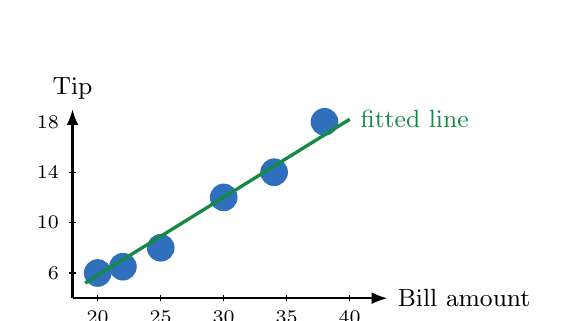
\begin{tikzpicture}[x=0.16cm,y=0.16cm,>=Latex]
  \draw[diagramAxis] (18,4) -- (43,4) node[right,font=\small]{Bill amount};
  \draw[diagramAxis] (18,4) -- (18,19) node[above,font=\small]{Tip};
  \foreach \x/\y in {20/6,22/6.5,25/8,30/12,34/14,38/18}{\fill[diagramBlue] (\x,\y) circle (5pt);}
  \draw[diagramGreen,very thick] (19,5.2) -- (40,18.2) node[right,font=\small]{fitted line};
  \foreach \x in {20,25,30,35,40}{\draw (\x,4.25)--(\x,3.75) node[below,font=\scriptsize]{\x};}
  \foreach \y in {6,10,14,18}{\draw (18.3,\y)--(17.7,\y) node[left,font=\scriptsize]{\y};}
\end{tikzpicture}
\end{center}


\subsection{Multiple Linear Regression}


\subsubsection{What is it?}


Multiple linear regression extends simple linear regression to include \textbf{two or more independent variables} simultaneously.

\textbf{Model equation:}

\[
\hat{y} = b_0 + b_1 x_1 + b_2 x_2 + \dots + b_k x_k
\]


Where \(k\) is the number of independent variables.

\textbf{Same intercept interpretation:} When all \(x_i = 0\), \(\hat{y} = b_0\).

\textbf{Slope interpretation (critical difference from simple regression):}

\begin{quote}
Each coefficient \(b_i\) represents the estimated change in Y for a \textbf{one-unit increase in \(x_i\)} when \textbf{all other independent variables are held constant}.
\end{quote}


\medskip


\subsubsection{Worked Example: Salary Prediction}


\textbf{Model:} \(\hat{y} = 27 + 9x_1 + 12x_2\) (all values in thousands of dollars)

\begin{itemize}[leftmargin=*]
    \item \(x_1\) = Capital investment (thousands)
    \item \(x_2\) = Marketing expenditure (thousands)
    \item \(\hat{y}\) = Predicted sales (thousands)

\end{itemize}

\textbf{Interpretation:}
\begin{itemize}[leftmargin=*]
    \item \textbf{\(b_0 = 27\):} When both capital investment and marketing spend are zero, expected sales = \$27,000.
    \item \textbf{\(b_1 = 9\):} For every \$1,000 increase in capital investment, sales increase by \textbf{\$9,000} --- \textit{holding marketing expenditure constant}.
    \item \textbf{\(b_2 = 12\):} For every \$1,000 increase in marketing spend, sales increase by \textbf{\$12,000} --- \textit{holding capital investment constant}.

\end{itemize}

\begin{quote}
The "holding all other variables constant" clause is essential. It allows us to isolate the unique contribution of each predictor.
\end{quote}


\medskip


\subsubsection{Worked Example: Regional Delivery Service}


\textbf{Problem:} Predict delivery trip duration (hours) using:
\begin{itemize}[leftmargin=*]
    \item \(X_1\) = Total miles traveled
    \item \(X_2\) = Number of deliveries during the trip

\end{itemize}

Sample of 10 trips (first 3 shown):

\begin{center}
\small
\renewcommand{\arraystretch}{1.15}
\begin{tabular}{|L{0.22\textwidth}|L{0.30\textwidth}|L{0.36\textwidth}|}
\hline
    Miles (\(X_1\)) & Deliveries (\(X_2\)) & Travel Time (\(Y\)) hours \\
\hline
    89 & 4 & 7.0 \\
\hline
    66 & 1 & 5.4 \\
\hline
    ... & ... & ... \\
\hline
\end{tabular}
\end{center}
\normalsize


\textbf{Why multiple regression?}
\begin{itemize}[leftmargin=*]
    \item Using only miles traveled captures some variation in trip duration.
    \item Adding number of deliveries may explain additional variation miles alone cannot account for.
    \item If both predictors help, the combined model reduces SSE more than either alone.

\end{itemize}

\medskip


\subsubsection{Two Critical Problems in Multiple Regression}


\paragraph{Problem 1: Overfitting}


Adding more independent variables always increases R\textsuperscript{2} (explains more variance) --- but can do so under \textbf{false pretenses}. Too many variables can cause a model to:
\begin{itemize}[leftmargin=*]
    \item Fit the training data perfectly (captures noise, not signal).
    \item Perform poorly on new, unseen data.

\end{itemize}

\begin{quote}
\textbf{The cure:} Select variables carefully. Include only those that are theoretically justified and statistically significant. More variables \(\neq\) better model.
\end{quote}


\paragraph{Problem 2: Multicollinearity}


Occurs when two or more independent variables are \textbf{strongly correlated with each other} --- they're measuring nearly the same thing.

\textbf{Why it's a problem:} If \(X_1\) and \(X_2\) are nearly identical, the model cannot separately determine \(b_1\) and \(b_2\). The regression equation becomes \textbf{unstable} --- small changes in data lead to drastically different coefficients.

\textbf{Analogy:} Adding sea salt and table salt to a recipe. You can taste "salty," but you can't tell which salt caused it.

\begin{quote}
\textbf{The ideal:} Independent variables are correlated with Y but \textbf{not} with each other.
\end{quote}


\textbf{Diagnosing multicollinearity --- the VIF approach:}

For each independent variable \(X_j\), run a regression where \(X_j\) is the dependent variable and all other \(X_i\) are the predictors. This gives a new \(R^2_j\).

\[
\text{Tolerance}_j = 1 - R^2_j
\]

\[
\text{VIF}_j = \frac{1}{\text{Tolerance}_j}
\]


\begin{center}
\small
\renewcommand{\arraystretch}{1.15}
\begin{tabular}{|L{0.28\textwidth}|L{0.60\textwidth}|}
\hline
    Value & Interpretation \\
\hline
    Tolerance \(<\) 0.1 & Potential multicollinearity problem \\
\hline
    VIF \(>\) 10 & Definite multicollinearity problem \\
\hline
\end{tabular}
\end{center}
\normalsize


\begin{quote}
If multicollinearity exists, coefficients cannot be meaningfully interpreted. However, if you only need predictions (not coefficient interpretation), multicollinearity does not affect predictive accuracy.
\end{quote}


\medskip




\subsubsection{Matrix Formulation of Multiple Regression}

Multiple regression is most clearly written in matrix notation. Let
\[
y=\begin{bmatrix}y_1\\y_2\\\vdots\\y_n\end{bmatrix},\qquad
X=\begin{bmatrix}
1&x_{11}&x_{12}&\cdots&x_{1k}\\
1&x_{21}&x_{22}&\cdots&x_{2k}\\
\vdots&\vdots&\vdots&\ddots&\vdots\\
1&x_{n1}&x_{n2}&\cdots&x_{nk}
\end{bmatrix},\qquad
\beta=\begin{bmatrix}\beta_0\\\beta_1\\\vdots\\\beta_k\end{bmatrix}.
\]
The population model is
\[
y=X\beta+\varepsilon.
\]
OLS chooses \(\hat{\beta}\) to minimize
\[
S(\beta)=(y-X\beta)'(y-X\beta).
\]
Differentiating and setting the gradient to zero gives the matrix normal equations:
\[
X'X\hat{\beta}=X'y.
\]
If \(X'X\) is invertible, meaning the columns of \(X\) are linearly independent, then
\[
\hat{\beta}=(X'X)^{-1}X'y.
\]
This is the exact multiple-regression analogue of the simple-regression formula \(b_1=S_{xy}/S_{xx}\).

\paragraph{Full rank condition.}
The matrix \(X'X\) fails to be invertible when one predictor is an exact linear combination of the others. This is the mathematical form of perfect multicollinearity. For example, including all dummy variables for every category plus an intercept creates a redundant column and makes \(X'X\) singular.

\subsubsection{Partial Regression and the Meaning of ``Holding Constant''}

The most important conceptual result in multiple regression is the \textbf{Frisch--Waugh--Lovell theorem}. It says that the coefficient on \(x_j\) can be obtained in three steps:
\begin{enumerate}[leftmargin=*]
    \item Regress \(x_j\) on all the other predictors and keep the residuals \(r_{x_j}\). These residuals are the part of \(x_j\) not explained by the other predictors.
    \item Regress \(y\) on all the other predictors and keep the residuals \(r_y\). These residuals are the part of \(y\) not explained by the other predictors.
    \item Regress \(r_y\) on \(r_{x_j}\). The slope from this regression is exactly the multiple-regression coefficient \(b_j\).
\end{enumerate}

\begin{quote}
\textbf{Meaning:} A multiple-regression coefficient is not the raw association between \(x_j\) and \(y\). It is the association between the leftover part of \(x_j\) and the leftover part of \(y\) after all other included variables have been removed.
\end{quote}


\begin{center}
\resizebox{0.95\textwidth}{!}{%
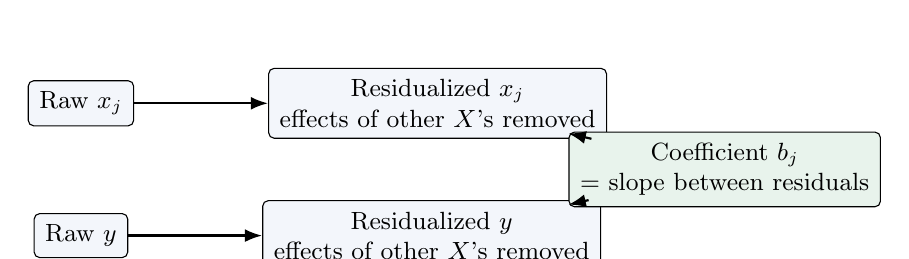
\begin{tikzpicture}[node distance=1.2cm and 1.7cm,>=Latex]
  \node[diagramBox] (xraw) {Raw \(x_j\)};
  \node[diagramBox,right=of xraw] (xres) {Residualized \(x_j\)\\effects of other \(X\)'s removed};
  \node[diagramBox,below=1.1cm of xraw] (yraw) {Raw \(y\)};
  \node[diagramBox,right=of yraw] (yres) {Residualized \(y\)\\effects of other \(X\)'s removed};
  \node[diagramBox,fill=diagramGreen!10,right=1.7cm of $(xres)!0.5!(yres)$] (slope) {Coefficient \(b_j\)\\= slope between residuals};
  \draw[diagramArrow] (xraw) -- (xres);
  \draw[diagramArrow] (yraw) -- (yres);
  \draw[diagramArrow] (xres) -- (slope);
  \draw[diagramArrow] (yres) -- (slope);
\end{tikzpicture}%
}
\end{center}


\subsubsection{Example: Interpreting Partial Effects}

For the salary-prediction model
\[
\hat{y}=27+9x_1+12x_2,
\]
where \(x_1\) is capital investment and \(x_2\) is marketing expenditure, both in thousands of dollars:
\begin{itemize}[leftmargin=*]
    \item Comparing two firms with the \textbf{same marketing spend}, increasing capital investment by \(1\) unit increases predicted sales by \(9\) units.
    \item Comparing two firms with the \textbf{same capital investment}, increasing marketing expenditure by \(1\) unit increases predicted sales by \(12\) units.
    \item If high-capital firms also tend to spend more on marketing, simple regression may confuse the two effects. Multiple regression separates them by residualizing each predictor against the other.
\end{itemize}

\paragraph{Interaction terms.}
Sometimes the effect of one variable depends on another. A model with interaction is
\[
\hat{y}=b_0+b_1x_1+b_2x_2+b_3x_1x_2.
\]
Then the marginal effect of \(x_1\) is not simply \(b_1\); it is
\[
\frac{\partial \hat{y}}{\partial x_1}=b_1+b_3x_2.
\]
In finance, this matters when the effect of volume on volatility changes during high-VIX regimes, or when the effect of leverage depends on interest rates.

\subsubsection{Inference in Multiple Regression}

With \(k\) predictors plus an intercept, the residual variance estimate is
\[
s^2=\frac{\text{SSE}}{n-k-1}.
\]
The covariance matrix of the OLS estimator is estimated by
\[
\widehat{\operatorname{Var}}(\hat{\beta})=s^2(X'X)^{-1}.
\]
The standard error of \(b_j\) is the square root of the \(j\)-th diagonal element of this matrix. Individual coefficient tests use
\[
t_j=\frac{b_j-0}{\operatorname{SE}(b_j)},
\]
with \(n-k-1\) degrees of freedom under the classical normal-error model.

\paragraph{Joint tests.}
To test several restrictions at once, such as
\[
H_0:\beta_2=\beta_3=\beta_4=0,
\]
use an \(F\)-test comparing a restricted model and an unrestricted model:
\[
F=\frac{(\text{SSE}_R-\text{SSE}_U)/q}{\text{SSE}_U/(n-k-1)},
\]
where \(q\) is the number of restrictions. This asks whether the added variables reduce SSE enough to justify their complexity.

\subsubsection{Adjusted \texorpdfstring{\(R^2\)}{R-squared}, AIC, and BIC}

Because ordinary \(R^2\) never decreases when a predictor is added, it can reward unnecessary complexity. Adjusted \(R^2\) penalizes the number of predictors:
\[
\bar{R}^2=1-\frac{\text{SSE}/(n-k-1)}{\text{SST}/(n-1)}.
\]
A variable improves adjusted \(R^2\) only if it reduces SSE enough to compensate for the lost degree of freedom.

Two common information criteria are
\begin{align*}
\text{AIC} &= n\ln\left(\frac{\text{SSE}}{n}\right)+2p,\\
\text{BIC} &= n\ln\left(\frac{\text{SSE}}{n}\right)+p\ln(n),
\end{align*}
where \(p=k+1\) is the number of estimated regression coefficients including the intercept. Lower AIC or BIC indicates a better trade-off between fit and complexity. BIC penalizes complexity more strongly than AIC when \(n\) is large.

\subsubsection{Diagnostics: Leverage, Influence, and Robust Standard Errors}

The fitted values can be written as
\[
\hat{y}=Hy, \qquad H=X(X'X)^{-1}X',
\]
where \(H\) is the \textbf{hat matrix}. Its diagonal entries \(h_{ii}\) are leverage scores.
\begin{itemize}[leftmargin=*]
    \item \textbf{High leverage:} an observation has unusual predictor values.
    \item \textbf{Large residual:} an observation is poorly predicted.
    \item \textbf{Influential point:} an observation has enough leverage and residual size to materially change the fitted coefficients.
\end{itemize}

A commonly used influence measure is Cook's distance:
\[
D_i=\frac{e_i^2}{(k+1)s^2}\cdot\frac{h_{ii}}{(1-h_{ii})^2}.
\]
Large values of \(D_i\) indicate observations that should be investigated, not automatically deleted.

If heteroscedasticity is present, OLS coefficients may remain unbiased under exogeneity, but the usual standard errors can be wrong. A common remedy is to keep the OLS coefficients and replace the covariance matrix with a heteroscedasticity-robust estimator:
\[
\widehat{\operatorname{Var}}_{\text{robust}}(\hat{\beta})=(X'X)^{-1}X'\widehat{\Omega}X(X'X)^{-1},
\]
where \(\widehat{\Omega}\) contains squared residual information on its diagonal.

\subsubsection{Practical Multiple-Regression Workflow}

\begin{enumerate}[leftmargin=*]
    \item \textbf{Define the target and predictors:} decide whether the goal is prediction, explanation, or causal inference.
    \item \textbf{Inspect data:} check missing values, outliers, units, and whether variables need transformations.
    \item \textbf{Fit a baseline model:} begin with theoretically justified variables rather than every available column.
    \item \textbf{Check diagnostics:} inspect residual plots, leverage, influence, multicollinearity, and heteroscedasticity.
    \item \textbf{Compare models:} use adjusted \(R^2\), cross-validation, AIC/BIC, or nested \(F\)-tests depending on the purpose.
    \item \textbf{Interpret carefully:} coefficients are conditional associations unless identification assumptions justify causal language.
\end{enumerate}

\subsection{Assumptions of Linear Regression}


If these assumptions are violated, regression results cannot be meaningfully interpreted.

\subsubsection{Assumption 1: Linearity}


\textbf{What it requires:} A linear relationship exists between each independent variable and the dependent variable.

\textbf{Why it matters:} Linear regression fits a straight line through data. If the true relationship is curved (non-linear), the straight line cannot represent the data well, leading to systematic errors in prediction.

\textbf{How to check:} Plot each independent variable against the dependent variable in a scatter plot. If the cloud of points curves, a straight line is not appropriate.


\begin{center}
\resizebox{0.92\textwidth}{!}{%
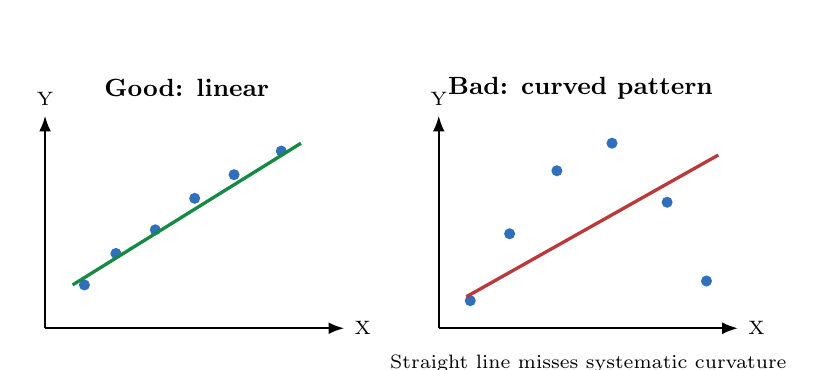
\begin{tikzpicture}[x=1cm,y=1cm,>=Latex]
  \foreach \x/\title in {0/{Good: linear},5/{Bad: curved pattern}}{
    \draw[diagramAxis] (\x,0) -- +(3.8,0) node[right,font=\scriptsize]{X};
    \draw[diagramAxis] (\x,0) -- +(0,2.7) node[above,font=\scriptsize]{Y};
    \node[font=\small\bfseries] at (\x+1.8,3.05) {\title};
  }
  \foreach \x/\y in {0.5/0.55,0.9/0.95,1.4/1.25,1.9/1.65,2.4/1.95,3.0/2.25}{\fill[diagramBlue] (\x,\y) circle (2pt);}
  \draw[diagramGreen,very thick] (0.35,0.55) -- (3.25,2.35);
  \foreach \x/\y in {5.4/0.35,5.9/1.2,6.5/2.0,7.2/2.35,7.9/1.6,8.4/0.6}{\fill[diagramBlue] (\x,\y) circle (2pt);}
  \draw[bearc,very thick] (5.35,0.4) -- (8.55,2.2);
  \node[font=\scriptsize,align=center] at (6.9,-0.45) {Straight line misses systematic curvature};
\end{tikzpicture}%
}
\end{center}



\textbf{Solutions if violated:} Transform variables (e.g., log transformation), use polynomial regression, or use a non-linear model.

\medskip


\subsubsection{Assumption 2: Normality of Errors}


\textbf{What it requires:} The residuals (\(\varepsilon\)) are normally distributed.

\textbf{Why it matters:} Many statistical tests (t-tests, F-tests) for regression coefficients assume normally distributed errors. Violations can make p-values unreliable.

\textbf{How to check:}

\textit{Analytical tests:}
\begin{itemize}[leftmargin=*]
    \item \textbf{Kolmogorov-Smirnov test} or \textbf{Shapiro-Wilk test}: If p \(>\) 0.05, normality is not rejected.
    \item Caveat: Analytical tests flag normality in small samples and reject it in large samples even for minor deviations. Use with caution.

\end{itemize}

\textit{Graphical tests (preferred):}
\begin{itemize}[leftmargin=*]
    \item \textbf{Histogram of residuals:} Should be bell-shaped.
    \item \textbf{QQ Plot (Quantile-Quantile Plot):} Plots residual quantiles against theoretical normal quantiles. If points lie on the diagonal line \(\rightarrow\) normally distributed. Deviations from the line indicate non-normality.

\end{itemize}

\medskip


\subsubsection{Assumption 3: Homoscedasticity}


\textbf{What it requires:} The variance of residuals is \textbf{constant} across all predicted values (homoscedasticity). The opposite problem is \textbf{heteroscedasticity}.

\textbf{Intuition:} The spread of residuals around the regression line should be the same regardless of where you are on the X-axis.


\begin{center}
\resizebox{0.95\textwidth}{!}{%
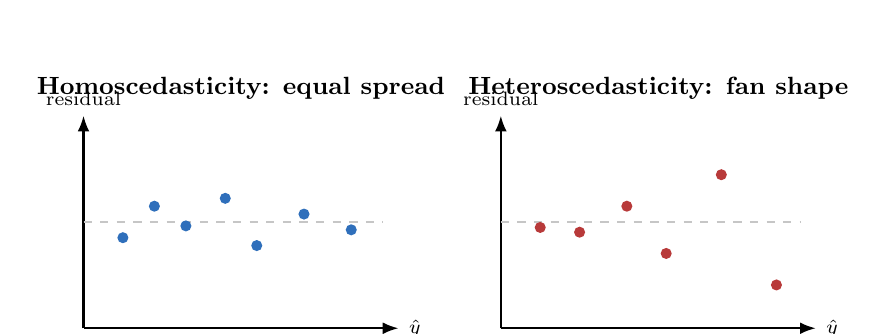
\begin{tikzpicture}[x=1cm,y=1cm,>=Latex]
  \foreach \x/\title in {0/{Homoscedasticity: equal spread},5.3/{Heteroscedasticity: fan shape}}{
    \draw[diagramAxis] (\x,0) -- +(4.0,0) node[right,font=\scriptsize]{\(\hat y\)};
    \draw[diagramAxis] (\x,0) -- +(0,2.7) node[above,font=\scriptsize]{residual};
    \draw[gray!45,dashed] (\x,1.35) -- +(3.8,0);
    \node[font=\small\bfseries] at (\x+2,3.05) {\title};
  }
  \foreach \x/\y in {0.5/1.15,0.9/1.55,1.3/1.3,1.8/1.65,2.2/1.05,2.8/1.45,3.4/1.25}{\fill[diagramBlue] (\x,\y) circle (2pt);}
  \foreach \x/\y in {5.8/1.28,6.3/1.22,6.9/1.55,7.4/0.95,8.1/1.95,8.8/0.55}{\fill[bearc] (\x,\y) circle (2pt);}
\end{tikzpicture}%
}
\end{center}



\textbf{How to check:} Plot predicted values (\(\hat{y}\)) on X-axis vs residuals on Y-axis. Residuals should scatter evenly (no fan shape, no funnel pattern).

\textbf{Solutions if violated:} Transform the dependent variable (log, square root), use weighted least squares, or use heteroscedasticity-robust standard errors.

\medskip


\subsubsection{Assumption 4: No Multicollinearity}


Already covered in Part 4. Use VIF \(<\) 10 and Tolerance \(>\) 0.1 as guidelines.

\textbf{When it matters most:} Only when using regression to \textit{measure} the influence of individual variables. For pure \textit{prediction}, multicollinearity doesn't affect predictive performance.

\medskip


\subsection{Dummy Variables}


\subsubsection{What and When}


Dummy variables are needed when you want to include a \textbf{categorical variable with more than 2 categories} as an independent variable in regression. Linear regression requires numeric inputs; dummy coding converts categories to 0/1 binary columns.

\subsubsection{Dichotomous Variables (2 categories)}


If a categorical variable already has exactly 2 values (e.g., gender: male/female), code one as 0 (reference category) and one as 1. The coefficient then represents the \textbf{difference between the two groups.}

\textbf{Example:}
\begin{itemize}[leftmargin=*]
    \item Gender coded: Female = 0, Male = 1
    \item Coefficient \(b_1 = 400\) \(\rightarrow\) men earn EUR 400 more than women (on average, per this model)
    \item For a female: \$1 \textbackslash{}times 0 = 0\$ (contributes nothing --- she is the reference)
    \item For a male: \$1 \textbackslash{}times 400 = 400\$ (add EUR 400 to salary prediction)

\end{itemize}

\subsubsection{More Than 2 Categories: Creating Dummy Variables}


\textbf{Rule: Create (n - 1) dummy variables for n categories.} One category is always dropped as the \textbf{reference category} (its values are implied when all other dummies = 0).

\textbf{Why n - 1?} If you know it's not a sedan AND not a sports car, it must be a family van --- that information is redundant. Including all n dummies would cause perfect multicollinearity.

\textbf{Example: Vehicle type with 3 categories}

\begin{center}
\scriptsize
\renewcommand{\arraystretch}{1.15}
\begin{tabular}{|L{0.14\textwidth}|L{0.06\textwidth}|L{0.13\textwidth}|L{0.15\textwidth}|L{0.20\textwidth}|}
\hline
    Original Variable & \(\rightarrow\) & Is it a Sedan? & Is it a Sports Car? & \textit{(Family Van dropped)} \\
\hline
    Sedan &  & 1 & 0 &  \\
\hline
    Sedan &  & 1 & 0 &  \\
\hline
    Sports Car &  & 0 & 1 &  \\
\hline
    Family Van &  & 0 & 0 & \(\leftarrow\) implied by both = 0 \\
\hline
\end{tabular}
\end{center}
\normalsize


The 2 dummy variables (Is\_Sedan, Is\_Sports\_Car) enter the regression model. Family Van is the reference category.

\textbf{Data preparation process:}

Starting with one column "Vehicle Type" \(\rightarrow\) create 2 new binary columns. For each observation, put 1 in the matching column and 0 in others.

\medskip


\subsection{Polynomial Regression}


\subsubsection{Why Not Always Use Linear Regression?}


Linear regression draws a \textbf{straight line} through data. But real-world relationships are not always linear. Consider:


\begin{center}
\resizebox{\textwidth}{!}{%
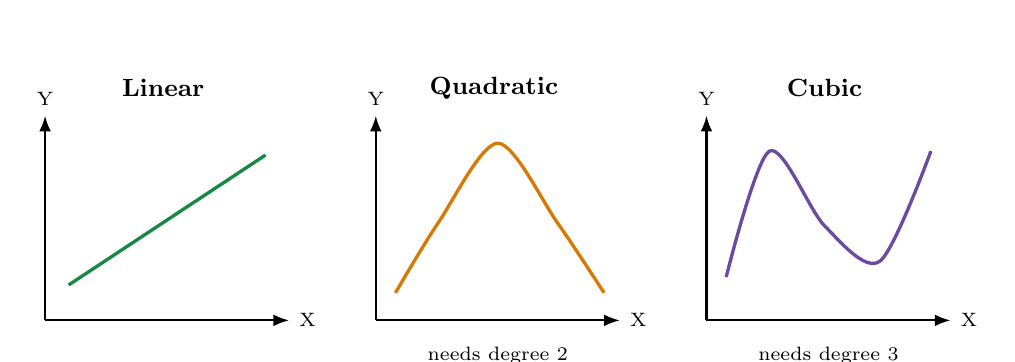
\begin{tikzpicture}[x=1cm,y=1cm,>=Latex]
  \foreach \x/\title in {0/{Linear},4.2/{Quadratic},8.4/{Cubic}}{
    \draw[diagramAxis] (\x,0) -- +(3.1,0) node[right,font=\scriptsize]{X};
    \draw[diagramAxis] (\x,0) -- +(0,2.6) node[above,font=\scriptsize]{Y};
    \node[font=\small\bfseries] at (\x+1.5,2.95) {\title};
  }
  \draw[diagramGreen,very thick] (0.3,0.45) -- (2.8,2.1);
  \draw[diagramOrange,very thick,smooth] plot coordinates {(4.45,0.35) (5.0,1.25) (5.75,2.25) (6.5,1.25) (7.1,0.35)};
  \draw[diagramPurple,very thick,smooth] plot coordinates {(8.65,0.55) (9.2,2.15) (9.9,1.2) (10.6,0.75) (11.25,2.15)};
  \node[font=\scriptsize,align=center] at (5.75,-0.45) {needs degree 2};
  \node[font=\scriptsize,align=center] at (9.95,-0.45) {needs degree 3};
\end{tikzpicture}%
}
\end{center}



\subsubsection{What is a Polynomial?}


A polynomial is an expression combining a variable raised to increasing powers with corresponding coefficients:

\[
P(x) = a_0 + a_1 x + a_2 x^2 + a_3 x^3 + \dots + a_n x^n
\]


The \textbf{order} (degree) of a polynomial is the \textbf{highest exponent present}, regardless of how many terms are included.

\subsubsection{Polynomial Regression Model}


\textbf{Degree 1 (Linear --- special case):}
\[
\hat{y} = \beta_0 + \beta_1 x + \varepsilon
\]


\textbf{Degree 2 (Quadratic):}
\[
\hat{y} = \beta_0 + \beta_1 x + \beta_2 x^2 + \varepsilon
\]


\textbf{Degree k (General):}
\[
\hat{y} = \beta_0 + \beta_1 x + \beta_2 x^2 + \dots + \beta_k x^k + \varepsilon
\]


\subsubsection{Why is Polynomial Regression Still "Linear"?}


Despite \(x^2\), \(x^3\) etc., polynomial regression is still a \textbf{General Linear Model}. The "linear" in linear regression refers to \textbf{linearity in the coefficients} (\(\beta_0, \beta_1, \beta_2, \dots\)), not in the variables. The coefficients are still being multiplied in a simple linear way --- only the \textit{data} (X values) get raised to powers, not the \textit{parameters}.

\textbf{In practice:} You create new variables \(X_2 = X^2\), \(X_3 = X^3\), etc., and run a standard multiple linear regression with these as additional predictors.

\subsubsection{Choosing the Right Degree: Bayes Information Criterion (BIC)}


Too low a degree \(\rightarrow\) underfitting (model too simple, misses the pattern).
Too high a degree \(\rightarrow\) overfitting (model captures noise, won't generalize).

\textbf{Bayes Information Criterion (BIC):}

\[
\text{BIC} = n \cdot \ln(\text{SSE}) + K \cdot \ln(n)
\]


Where:
\begin{itemize}[leftmargin=*]
    \item \(n\) = number of data points
    \item SSE = Sum of Squared Errors for the polynomial of degree K
    \item \(K\) = number of parameters (degree + 1)

\end{itemize}

\textbf{Method:}
\begin{enumerate}[leftmargin=*]
    \item Fit polynomial models for degrees 1, 2, 3, ..., up to some maximum.
    \item Calculate BIC for each.
    \item Choose the degree with the \textbf{lowest BIC} --- it balances fit quality and model complexity.

\end{enumerate}


\begin{center}
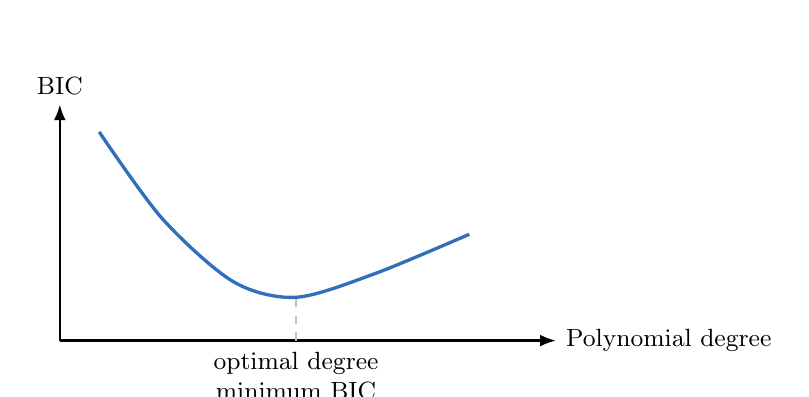
\begin{tikzpicture}[x=1cm,y=1cm,>=Latex]
  \draw[diagramAxis] (0,0) -- (6.3,0) node[right,font=\small]{Polynomial degree};
  \draw[diagramAxis] (0,0) -- (0,3.0) node[above,font=\small]{BIC};
  \draw[diagramBlue,very thick,smooth] plot coordinates {(0.5,2.65) (1.3,1.55) (2.2,0.75) (3.0,0.55) (4.0,0.85) (5.2,1.35)};
  \draw[gray!50,dashed] (3.0,0) -- (3.0,0.55);
  \node[font=\small,align=center] at (3.0,-0.45) {optimal degree\\minimum BIC};
\end{tikzpicture}
\end{center}



\subsubsection{Python Implementation (Overview)}


Using STEM salaries data with features: years of experience, years at company, base salary \(\rightarrow\) predicting total yearly compensation.

\begin{Verbatim}[breaklines=true,fontsize=\small]
# Key steps:
# 1. For each degree i (1 to 5):
#    a. Create polynomial feature matrix:
#       X_1, X_2, X_3 -> X_1, X_1^2, X_2, X_2^2, X_3, X_3^2 (for degree 2)
#    b. Use linear algebra (least squares) to find weights W
#       W = (X^TX)^-^1 X^Ty
#    c. Predict: yhat = X . W
#    d. Calculate RMSE for training and testing sets
#    e. Store in dictionary

# 2. Plot training error vs testing error across degrees
\end{Verbatim}


\textbf{Key observation:} As polynomial degree increases:
\begin{itemize}[leftmargin=*]
    \item \textbf{Training error} consistently increases (more parameters = harder to fit training data).
    \item \textbf{Testing error} may decrease slightly then increase (overfitting risk).

\end{itemize}

\textbf{Root Mean Squared Error (RMSE):}

\[
\text{RMSE} = \sqrt{\frac{1}{n}\sum_{i=1}^{n}(y_i - \hat{y}_i)^2}
\]


The polynomial degree with the \textbf{lowest testing RMSE} (or BIC) is the optimal choice.

\medskip


\subsection{Ridge Regression}


\subsubsection{The Problem: Overfitting with Steep Slopes}


Consider a training dataset with only 2 points. A linear regression model will fit a line passing through both points perfectly --- zero training error. But this line may have a very steep slope.

When tested on new data:
\begin{itemize}[leftmargin=*]
    \item The steep slope causes large errors for data points not on the original line.
    \item This is \textbf{overfitting}: Low bias on training data, high variance on test data.

\end{itemize}

\textbf{Overfitting = Low training error + High test error}

The problem is fundamentally that overfitted models have \textbf{large slope coefficients} --- with one unit of X, Y changes dramatically. This makes the model extremely sensitive to small variations in input.

\subsubsection{Ridge Regression Cost Function}


Standard linear regression minimizes:

\[
\text{Cost} = \sum_{i=1}^{n}(y_i - \hat{y}_i)^2 \quad (\text{Sum of Squared Errors})
\]


\textbf{Ridge regression} adds a \textbf{penalty term} (L2 regularization):

\[
\text{Cost}_{\text{Ridge}} = \underbrace{\sum_{i=1}^{n}(y_i - \hat{y}_i)^2}_{\text{Sum of Squared Errors}} + \underbrace{\lambda \sum_{j=1}^{k} m_j^2}_{\text{L2 Penalty (Ridge Penalty)}}
\]


Where:
\begin{itemize}[leftmargin=*]
    \item \(\lambda\) (lambda) = regularization hyperparameter (always \(\geq\) 0)
    \item \(m_j\) = slope coefficient for predictor \(j\)
    \item \(m_j^2\) = squared slope

\end{itemize}

\textbf{With multiple features (\(k\) predictors):}

\[
\text{Cost}_{\text{Ridge}} = \sum(y - \hat{y})^2 + \lambda(m_1^2 + m_2^2 + \dots + m_k^2)
\]


\subsubsection{How Ridge Regression Reduces Overfitting}


\textbf{Intuition:} If a coefficient \(m_j\) is very large (steep slope \(\rightarrow\) overfitting), the penalty \(\lambda m_j^2\) becomes large, making the total cost large. The optimization then seeks a \textit{less steep line} that produces a slightly higher SSE but a much lower penalty, resulting in a lower total cost.

\textbf{Step-by-step logic:}
\begin{enumerate}[leftmargin=*]
    \item Steep line: SSE = 0 (perfect fit on training data), Penalty = \(\lambda\) \(\times\) (1.3)\textsuperscript{2} = 1.69 \(\rightarrow\) Total = 1.69.
    \item Less steep line: SSE = small value, Penalty = \(\lambda\) \(\times\) (1.0)\textsuperscript{2} = 1.0 \(\rightarrow\) Total = 1 + small \(<\) 1.69.
    \item Algorithm chooses the less steep line because total cost is lower.
    \item Result: A more \textbf{generalized} model with slight training bias but much better test performance.

\end{enumerate}

\subsubsection{Effect of Lambda (\(\lambda\)) --- Visual Intuition}


Ridge regression modifies the parabola of squared residuals:


\begin{center}
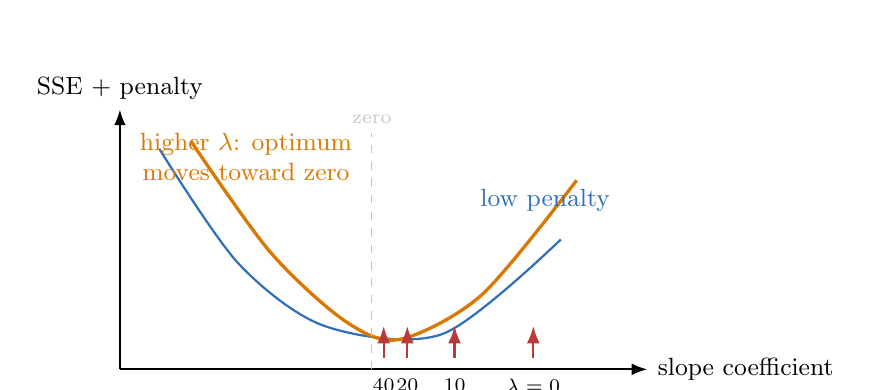
\begin{tikzpicture}[x=1cm,y=1cm,>=Latex]
  \draw[diagramAxis] (-3.2,0) -- (3.5,0) node[right,font=\small]{slope coefficient};
  \draw[diagramAxis] (-3.2,0) -- (-3.2,3.3) node[above,font=\small]{SSE + penalty};
  \draw[diagramBlue,thick,smooth] plot coordinates {(-2.7,2.8) (-1.7,1.35) (-0.6,0.55) (0.9,0.45) (2.4,1.65)};
  \draw[diagramOrange,very thick,smooth] plot coordinates {(-2.3,2.9) (-1.3,1.5) (-0.35,0.62) (0.35,0.38) (1.4,0.95) (2.6,2.4)};
  \draw[gray!45,dashed] (0,0) -- (0,3.0) node[above,font=\scriptsize]{zero};
  \foreach \x/\lab in {2.05/\(\lambda=0\),1.05/10,0.45/20,0.15/40}{\draw[diagramArrow,bearc] (\x,0.15) -- (\x,0.55); \node[font=\scriptsize,below] at (\x,0) {\lab};}
  \node[font=\small,diagramBlue] at (2.2,2.15) {low penalty};
  \node[font=\small,diagramOrange,align=center] at (-1.6,2.7) {higher \(\lambda\): optimum\\moves toward zero};
\end{tikzpicture}
\end{center}



\begin{quote}
\textbf{Key property of Ridge:} Coefficients are \textbf{shrunk toward zero} but \textbf{never reach exactly zero}. All features are retained; they just have smaller influence.
\end{quote}


\subsubsection{\(\lambda\) Selection}


\begin{itemize}[leftmargin=*]
    \item \textbf{\(\lambda\) = 0:} No penalty \(\rightarrow\) same as ordinary least squares (OLS). May overfit.
    \item \textbf{\(\lambda\) \(\rightarrow\) \(\infty\):} All coefficients approach zero \(\rightarrow\) underfitting (a flat horizontal line).
    \item \textbf{Optimal \(\lambda\):} Found via cross-validation. The best \(\lambda\) balances bias and variance.

\end{itemize}

\medskip


\subsection{Lasso Regression}


\subsubsection{What is it?}


Lasso (Least Absolute Shrinkage and Selection Operator) is similar to Ridge but uses an \textbf{L1 penalty} (absolute value instead of squared):

\[
\text{Cost}_{\text{Lasso}} = \underbrace{\sum_{i=1}^{n}(y_i - \hat{y}_i)^2}_{\text{Sum of Squared Errors}} + \underbrace{\lambda \sum_{j=1}^{k} |m_j|}_{\text{L1 Penalty (Lasso Penalty)}}
\]


\textbf{With multiple features:}

\[
\text{Cost}_{\text{Lasso}} = \sum(y - \hat{y})^2 + \lambda(|m_1| + |m_2| + \dots + |m_k|)
\]


\subsubsection{Key Difference: Lasso Can Set Coefficients Exactly to Zero}


The critical distinction between Ridge (L2) and Lasso (L1) is their behavior as \(\lambda\) increases:


\begin{center}
\resizebox{0.9\textwidth}{!}{%
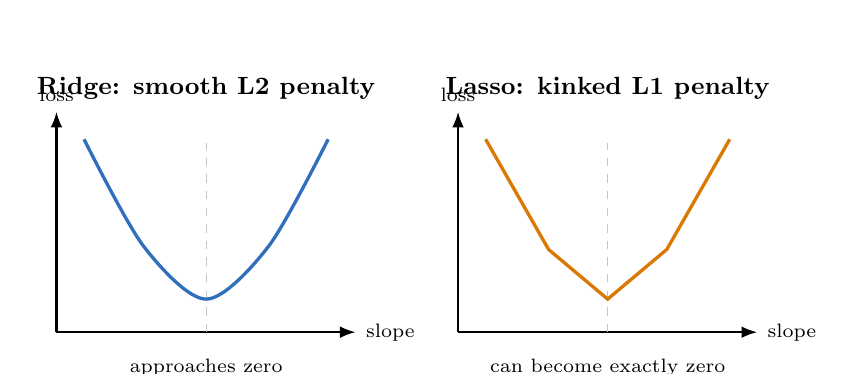
\begin{tikzpicture}[x=1cm,y=1cm,>=Latex]
  \foreach \x/\title in {0/{Ridge: smooth L2 penalty},5.1/{Lasso: kinked L1 penalty}}{
    \draw[diagramAxis] (\x,0) -- +(3.8,0) node[right,font=\scriptsize]{slope};
    \draw[diagramAxis] (\x,0) -- +(0,2.8) node[above,font=\scriptsize]{loss};
    \draw[gray!45,dashed] (\x+1.9,0) -- +(0,2.4);
    \node[font=\small\bfseries] at (\x+1.9,3.1) {\title};
  }
  \draw[diagramBlue,very thick,smooth] plot coordinates {(0.35,2.45) (1.1,1.1) (1.9,0.42) (2.7,1.1) (3.45,2.45)};
  \draw[diagramOrange,very thick] (5.45,2.45) -- (6.25,1.05) -- (7.0,0.42) -- (7.75,1.05) -- (8.55,2.45);
  \node[font=\scriptsize,align=center] at (1.9,-0.45) {approaches zero};
  \node[font=\scriptsize,align=center] at (7.0,-0.45) {can become exactly zero};
\end{tikzpicture}%
}
\end{center}



The absolute value function creates a \textbf{kink at zero}. When \(\lambda\) is large enough, the minimum of the total cost function sits exactly at slope = 0, which means that feature is \textbf{completely removed} from the model.

\subsubsection{Lasso as Feature Selection}


When some slope coefficients become exactly zero, those features are effectively \textbf{removed from the model}. Lasso automatically performs \textbf{feature selection} --- it identifies which predictors are irrelevant and excludes them.

\textbf{Example with 4 features:}

\[
\hat{y} = m_1 x_1 + m_2 x_2 + m_3 x_3 + m_4 x_4 + c
\]


After Lasso with sufficient \(\lambda\):

\[
\hat{y} = m_1 x_1 + 0 \cdot x_2 + m_3 x_3 + 0 \cdot x_4 + c = m_1 x_1 + m_3 x_3 + c
\]


Features \(x_2\) and \(x_4\) are eliminated because their slopes became zero --- they were not important for prediction.

\subsubsection{Ridge vs. Lasso: Summary Comparison}


\begin{center}
\small
\renewcommand{\arraystretch}{1.15}
\begin{tabular}{|L{0.22\textwidth}|L{0.30\textwidth}|L{0.36\textwidth}|}
\hline
    Feature & Ridge (L2) & Lasso (L1) \\
\hline
    \textbf{Penalty type} & \(\lambda \sum m_j^2\) (squared) & \(\lambda \sum |m_j|\) (absolute value) \\
\hline
    \textbf{Shape at zero} & Smooth parabola, no kink & Kink at zero \\
\hline
    \textbf{Coefficients reach exactly zero?} & Never --- only approach zero & Yes --- some become exactly zero \\
\hline
    \textbf{Feature selection?} & No --- all features retained (shrunk) & Yes --- can eliminate features \\
\hline
    \textbf{Best use case} & When all features are relevant, reduce their influence & When some features are irrelevant, eliminate them \\
\hline
    \textbf{Multicollinearity} & Handles better than OLS & Can arbitrarily select one from correlated features \\
\hline
    \textbf{As \(\lambda\) \(\rightarrow\) \(\infty\)} & Coefficients \(\rightarrow\) 0 (but never = 0) & Coefficients = 0 (explicitly) \\
\hline
\end{tabular}
\end{center}
\normalsize


\subsubsection{Both Reduce Overfitting By:}


\begin{enumerate}[leftmargin=*]
    \item \textbf{Penalizing steep slopes} --- preventing any single coefficient from becoming too large.
    \item \textbf{Introducing a trade-off} --- sacrificing some training accuracy (more bias) for better generalization (less variance).
    \item \textbf{Converting high-variance models into more generalized models} --- the goal is a model with both low bias AND low variance.

\end{enumerate}

\medskip


\subsection{Logistic Regression}


\subsubsection{Why Not Linear Regression for Binary Outcomes?}


Consider predicting whether a bank will approve a mortgage (1 = approved, 0 = not approved) based on credit score.

\textbf{Problem with linear regression:}
\begin{enumerate}[leftmargin=*]
    \item Linear regression can produce predicted values outside [0, 1] (e.g., predicting -0.3 or 1.7 probability --- meaningless).
    \item Binary data (0/1) does not have a normal distribution --- violates the normality assumption.
    \item The relationship between credit score and approval probability is S-shaped, not linear.

\end{enumerate}


\begin{center}
\resizebox{\textwidth}{!}{%
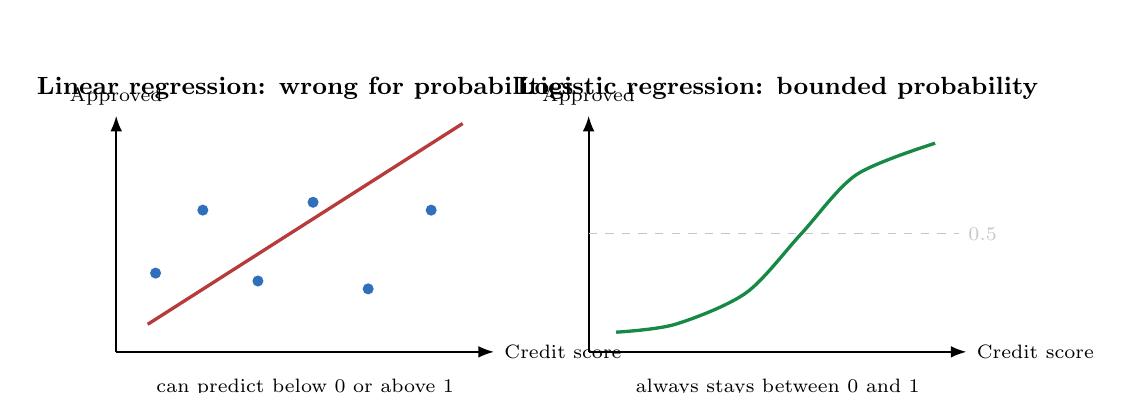
\begin{tikzpicture}[x=1cm,y=1cm,>=Latex]
  \foreach \x/\title in {0/{Linear regression: wrong for probabilities},6/{Logistic regression: bounded probability}}{
    \draw[diagramAxis] (\x,0) -- +(4.8,0) node[right,font=\scriptsize]{Credit score};
    \draw[diagramAxis] (\x,0) -- +(0,3.0) node[above,font=\scriptsize]{Approved};
    \node[font=\small\bfseries,align=center] at (\x+2.4,3.35) {\title};
  }
  \foreach \x/\y in {0.5/0.2,1.1/1.0,1.8/0.1,2.5/1.1,3.2/0.0,4.0/1.0}{\fill[diagramBlue] (\x,\y+0.8) circle (2pt);}
  \draw[bearc,very thick] (0.4,0.35) -- (4.4,2.9);
  \draw[diagramGreen,very thick,smooth] plot coordinates {(6.35,0.25) (7.1,0.35) (8.0,0.75) (8.7,1.5) (9.4,2.25) (10.4,2.65)};
  \draw[gray!45,dashed] (6,1.5)--(10.7,1.5) node[right,font=\scriptsize]{0.5};
  \node[font=\scriptsize,align=center] at (2.4,-0.45) {can predict below 0 or above 1};
  \node[font=\scriptsize,align=center] at (8.4,-0.45) {always stays between 0 and 1};
\end{tikzpicture}%
}
\end{center}



\subsubsection{The Logistic (Sigmoid) Function}


Logistic regression uses the \textbf{sigmoid function} to map any real number to a probability between 0 and 1:

\[
P(y=1|x) = \frac{1}{1 + e^{-z}}
\]


Where:

\[
z = \beta_0 + \beta_1 x_1 + \beta_2 x_2 + \dots + \beta_k x_k
\]


\textbf{Properties of the sigmoid:}
\begin{itemize}[leftmargin=*]
    \item When \(z \to +\infty\): \(P \to 1\)
    \item When \(z \to -\infty\): \(P \to 0\)
    \item When \(z = 0\): \(P = 0.5\)
    \item Always between 0 and 1

\end{itemize}


\begin{center}
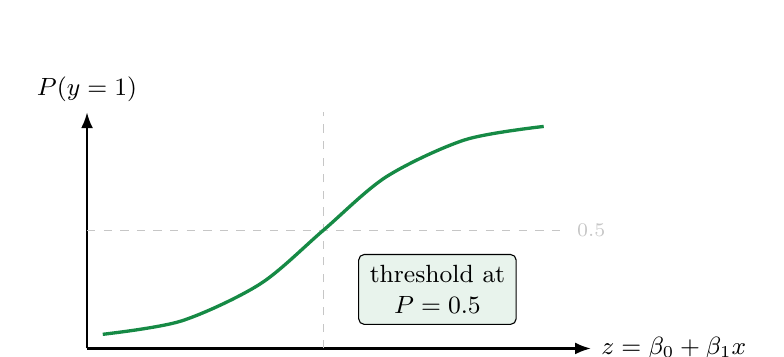
\begin{tikzpicture}[x=1cm,y=1cm,>=Latex]
  \draw[diagramAxis] (-3,0) -- (3.4,0) node[right,font=\small]{\(z=\beta_0+\beta_1x\)};
  \draw[diagramAxis] (-3,0) -- (-3,3.0) node[above,font=\small]{\(P(y=1)\)};
  \draw[gray!45,dashed] (-3,1.5)--(3.1,1.5) node[right,font=\scriptsize]{0.5};
  \draw[gray!45,dashed] (0,0)--(0,3);
  \draw[diagramGreen,very thick,smooth] plot coordinates {(-2.8,0.18) (-1.8,0.35) (-0.8,0.82) (0,1.5) (0.8,2.18) (1.8,2.65) (2.8,2.82)};
  \node[diagramBox,fill=diagramGreen!10] at (1.45,0.75) {threshold at\\\(P=0.5\)};
\end{tikzpicture}
\end{center}



\subsubsection{From Logit to Sigmoid: The Math}


The logistic regression model is built on \textbf{log-odds (logit)}:

\[
\ln\left(\frac{P}{1-P}\right) = \beta_0 + \beta_1 x_1 + \dots + \beta_k x_k
\]


Where:
\begin{itemize}[leftmargin=*]
    \item \(\frac{P}{1-P}\) = odds (probability of event / probability of no event)
    \item \(\ln\left(\frac{P}{1-P}\right)\) = log-odds (logit)

\end{itemize}

\textbf{Solving for P (inverting the logit):}

\[
\frac{P}{1-P} = e^z \implies P = \frac{e^z}{1 + e^z} = \frac{1}{1 + e^{-z}} \quad \text{(Sigmoid function)}
\]


\subsubsection{Classification Using Logistic Regression}


After computing the probability P, classify using a \textbf{decision boundary (threshold)}:

\begin{itemize}[leftmargin=*]
    \item If \(P \geq 0.5\) \(\rightarrow\) classify as class 1 (e.g., approved)
    \item If \(P < 0.5\) \(\rightarrow\) classify as class 0 (e.g., not approved)

\end{itemize}

The threshold of 0.5 can be adjusted based on the problem's requirements (e.g., for medical screening, you might use 0.3 to reduce false negatives).

\subsubsection{Maximum Likelihood Estimation (MLE)}


Logistic regression cannot use least squares (since there are no residuals in the traditional sense). Instead, it uses \textbf{Maximum Likelihood Estimation}:

\textbf{Process:}
\begin{enumerate}[leftmargin=*]
    \item Choose a sigmoid curve (a set of \(\beta\) values).
    \item Calculate the probability of observing each actual data point given that curve.
    \item Multiply all probabilities together \(\rightarrow\) this is the \textbf{Likelihood} of the data given those \(\beta\) values.
    \item Shift the curve and recalculate likelihood.
    \item Repeat until the curve with the \textbf{maximum likelihood} is found.

\end{enumerate}

\begin{Verbatim}[breaklines=true,fontsize=\small]
Likelihood = P(observe data | model parameters beta)

Goal: Find beta values that MAXIMIZE this likelihood
-> The resulting sigmoid curve best explains the observed data
\end{Verbatim}


\subsubsection{Types of Logistic Regression}


\begin{center}
\small
\renewcommand{\arraystretch}{1.15}
\begin{tabular}{|L{0.22\textwidth}|L{0.30\textwidth}|L{0.36\textwidth}|}
\hline
    Type & Dependent Variable & Example \\
\hline
    \textbf{Binary} & 2 outcomes (0/1) & Approved/Not approved, Spam/Not spam \\
\hline
    \textbf{Multinomial} & 3+ unordered outcomes & Buy Product A / B / C \\
\hline
    \textbf{Ordinal} & 3+ ordered outcomes & Customer rating: 1, 2, 3, 4, 5 (ordered) \\
\hline
\end{tabular}
\end{center}
\normalsize


\subsubsection{Applications}


\begin{itemize}[leftmargin=*]
    \item \textbf{Finance:} Fraud detection, mortgage approval, credit default prediction
    \item \textbf{Healthcare:} Disease diagnosis, cancer prediction, drug response
    \item \textbf{Marketing:} Customer churn prediction, product purchase likelihood
    \item \textbf{Politics:} Voter behavior prediction
    \item \textbf{Tech:} Email spam classification, image classification

\end{itemize}

\subsubsection{Assumptions for Logistic Regression}


\begin{enumerate}[leftmargin=*]
    \item Dependent variable must be binary (for binary logistic regression).
    \item Only relevant independent variables should be included.
    \item \textbf{No multicollinearity} among independent variables.
    \item \textbf{Large sample sizes} required (rule of thumb: \(\geq\) 10 events per predictor).
    \item \textbf{Linearity in log-odds}: The log-odds should be linearly related to continuous predictors.

\end{enumerate}

\subsubsection{Decision Boundary (Linear and Non-linear)}


The decision boundary is the set of points where P = 0.5 (i.e., the threshold). With one predictor, it's a point. With two predictors, it's a line. Polynomial features can create non-linear decision boundaries.


\begin{center}
\resizebox{\textwidth}{!}{%
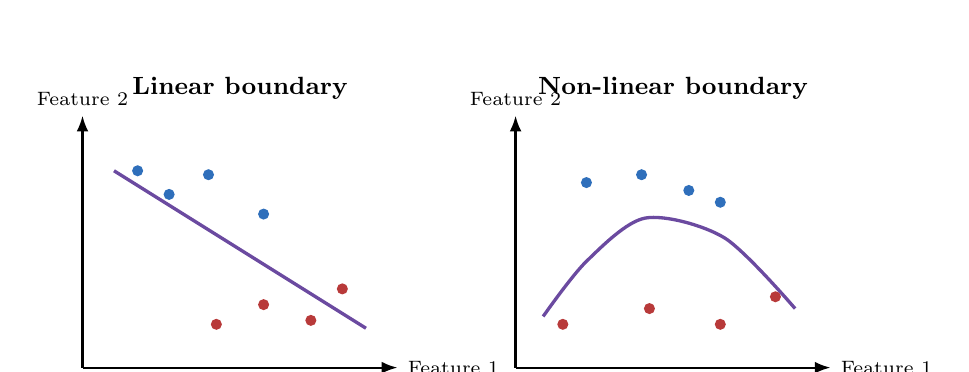
\begin{tikzpicture}[x=1cm,y=1cm,>=Latex]
  \foreach \x/\title in {0/{Linear boundary},5.5/{Non-linear boundary}}{
    \draw[diagramAxis] (\x,0) -- +(4,0) node[right,font=\scriptsize]{Feature 1};
    \draw[diagramAxis] (\x,0) -- +(0,3.2) node[above,font=\scriptsize]{Feature 2};
    \node[font=\small\bfseries] at (\x+2,3.55) {\title};
  }
  \draw[diagramPurple,very thick] (0.4,2.5) -- (3.6,0.5);
  \foreach \x/\y in {0.7/2.5,1.1/2.2,1.6/2.45,2.3/1.95}{\fill[diagramBlue] (\x,\y) circle (2pt);}
  \foreach \x/\y in {1.7/0.55,2.3/0.8,2.9/0.6,3.3/1.0}{\fill[bearc] (\x,\y) circle (2pt);}
  \draw[diagramPurple,very thick,smooth] plot coordinates {(5.85,0.65) (6.4,1.35) (7.15,1.9) (8.15,1.65) (9.05,0.75)};
  \foreach \x/\y in {6.4/2.35,7.1/2.45,7.7/2.25,8.1/2.1}{\fill[diagramBlue] (\x,\y) circle (2pt);}
  \foreach \x/\y in {6.1/0.55,7.2/0.75,8.1/0.55,8.8/0.9}{\fill[bearc] (\x,\y) circle (2pt);}
\end{tikzpicture}%
}
\end{center}



\subsubsection{Cost Function: Log-Loss (Cross-Entropy)}


Because MSE would create a non-convex surface for logistic regression (multiple local minima), a different cost function is used:

\textbf{For a single observation:}
\begin{itemize}[leftmargin=*]
    \item If actual \(y = 1\): Cost = \(-\ln(P)\) --- large cost when P is close to 0 (incorrectly confident)
    \item If actual \(y = 0\): Cost = \(-\ln(1 - P)\) --- large cost when P is close to 1

\end{itemize}

\textbf{Combined formula:}

\[
\text{Cost} = -\frac{1}{n}\sum_{i=1}^{n}\left[y_i \ln(\hat{P}_i) + (1-y_i)\ln(1-\hat{P}_i)\right]
\]


This is convex \(\rightarrow\) gradient descent can reliably find the global minimum.

\subsubsection{Regularization in Logistic Regression}


Just like in linear regression, logistic regression can overfit with many features:

\begin{itemize}[leftmargin=*]
    \item \textbf{L1 (Lasso):} \(\text{Cost} + \lambda\sum|\beta_j|\) \(\rightarrow\) can set coefficients to zero (feature selection)
    \item \textbf{L2 (Ridge):} \(\text{Cost} + \lambda\sum\beta_j^2\) \(\rightarrow\) shrinks coefficients (reduces multicollinearity)

\end{itemize}

In sklearn, controlled by the \texttt{C} parameter: C = 1/\(\lambda\) (higher C = less regularization).

\subsubsection{Connection to Neural Networks}


A single neuron in a neural network performs: dot product of inputs and weights \(\rightarrow\) non-linear activation function. This is \textbf{exactly} logistic regression. A multi-layer neural network is essentially many stacked logistic regression models:


\begin{center}
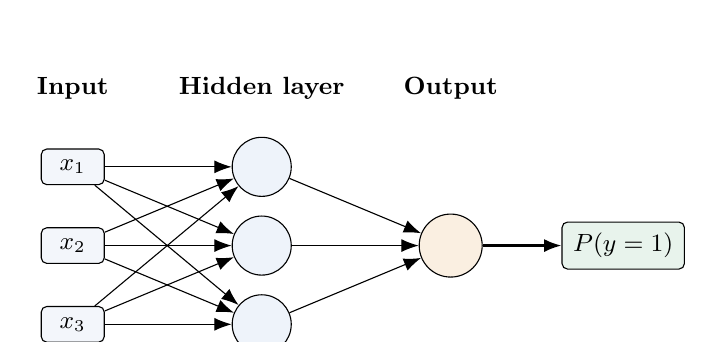
\begin{tikzpicture}[node distance=1.1cm and 1.5cm,>=Latex]
  \foreach \i/\lab in {1/\(x_1\),2/\(x_2\),3/\(x_3\)}{\node[diagramBox,minimum width=0.8cm] (x\i) at (0,-\i) {\lab};}
  \foreach \i in {1,2,3}{\node[circle,draw,fill=diagramBlue!8,minimum size=0.75cm] (h\i) at (2.4,-\i) {};}
  \node[circle,draw,fill=diagramOrange!12,minimum size=0.8cm] (o) at (4.8,-2) {};
  \node[diagramBox,fill=diagramGreen!10,right=1.0cm of o] (p) {\(P(y=1)\)};
  \foreach \i in {1,2,3}{\foreach \j in {1,2,3}{\draw[diagramArrow,thin] (x\i) -- (h\j);}}
  \foreach \j in {1,2,3}{\draw[diagramArrow,thin] (h\j) -- (o);}
  \draw[diagramArrow] (o) -- (p);
  \node[font=\small\bfseries] at (0,0) {Input};
  \node[font=\small\bfseries] at (2.4,0) {Hidden layer};
  \node[font=\small\bfseries] at (4.8,0) {Output};
\end{tikzpicture}
\end{center}



The last layer is a logistic regression. The hidden layers learn rich data representations. This is why logistic regression is the foundational building block of deep learning.

\subsubsection{Advantages of Logistic Regression}


\begin{itemize}[leftmargin=*]
    \item Simple, interpretable, fast to train
    \item Naturally outputs probabilities
    \item Less prone to overfitting on low-dimensional data
    \item Works well when features are roughly linearly separable
    \item Easy to extend to multi-class problems

\end{itemize}

\subsubsection{Disadvantages}


\begin{itemize}[leftmargin=*]
    \item Cannot model complex non-linear relationships (needs feature engineering)
    \item Sensitive to outliers
    \item Assumes linearity in log-odds
    \item Requires large samples for reliable estimates
    \item Poor performance when categories are not linearly separable

\end{itemize}

\medskip




\subsubsection{Logistic Regression as a Bernoulli Generalized Linear Model}

For binary outcomes, each observation is modeled as
\[
Y_i\mid x_i \sim \operatorname{Bernoulli}(p_i), \qquad p_i=P(Y_i=1\mid x_i).
\]
Logistic regression connects the probability \(p_i\) to a linear index \(z_i=x_i'\beta\) through the logit link:
\[
\log\left(\frac{p_i}{1-p_i}\right)=x_i'\beta.
\]
Equivalently,
\[
p_i=\frac{1}{1+e^{-x_i'\beta}}.
\]
This is a \textbf{generalized linear model} because:
\begin{itemize}[leftmargin=*]
    \item the conditional distribution is Bernoulli rather than normal;
    \item the conditional mean is \(E[Y_i\mid x_i]=p_i\);
    \item a link function, the logit, transforms the mean into a linear expression.
\end{itemize}

\begin{Verbatim}[breaklines=true,fontsize=\small]
Linear score z = beta_0 + beta_1 x_1 + ... + beta_k x_k
          |
          v
Sigmoid converts score to probability in [0,1]
          |
          v
Decision rule converts probability to class label
\end{Verbatim}

\subsubsection{Likelihood, Log-Likelihood, Gradient, and Hessian}

For one observation, the Bernoulli probability mass function can be written compactly as
\[
P(Y_i=y_i\mid x_i)=p_i^{y_i}(1-p_i)^{1-y_i}.
\]
Assuming independent observations, the likelihood is
\[
L(\beta)=\prod_{i=1}^{n}p_i^{y_i}(1-p_i)^{1-y_i}.
\]
The log-likelihood is easier to optimize:
\[
\ell(\beta)=\sum_{i=1}^{n}\left[y_i\log(p_i)+(1-y_i)\log(1-p_i)\right].
\]
The negative average log-likelihood is exactly the log-loss already shown:
\[
J(\beta)=-\frac{1}{n}\ell(\beta).
\]

Let \(X\) be the design matrix, \(p\) the vector of predicted probabilities, and \(y\) the vector of observed outcomes. The gradient of the log-likelihood is
\[
\nabla \ell(\beta)=X'(y-p).
\]
At the maximum likelihood estimate, the score equations satisfy
\[
X'(y-\hat{p})=0.
\]
This resembles the OLS normal equations: fitted errors are orthogonal to the predictors, but here the residuals are probability residuals \(y_i-\hat{p}_i\).

The Hessian is
\[
\nabla^2\ell(\beta)=-X'WX,
\]
where \(W\) is diagonal with entries \(w_i=p_i(1-p_i)\). Since \(W\) is nonnegative, \(-\ell(\beta)\) is convex. This is why logistic regression has a well-behaved optimization problem when the data are not perfectly separated.

\subsubsection{Optimization: Newton--Raphson and IRLS}

Logistic regression has no closed-form solution like OLS. A standard algorithm is Newton--Raphson:
\[
\beta^{(t+1)}=\beta^{(t)}-\left[\nabla^2\ell(\beta^{(t)})\right]^{-1}\nabla\ell(\beta^{(t)}).
\]
Using the logistic gradient and Hessian, this becomes an iteratively reweighted least squares (IRLS) procedure:
\[
\beta^{(t+1)}=(X'W^{(t)}X)^{-1}X'W^{(t)}z^{(t)},
\]
where \(W^{(t)}\) contains \(p_i^{(t)}(1-p_i^{(t)})\) and \(z^{(t)}\) is a working response. The intuition is that each iteration solves a weighted least-squares problem that approximates the curved log-likelihood near the current coefficient values.


\begin{center}
\resizebox{0.72\textwidth}{!}{%
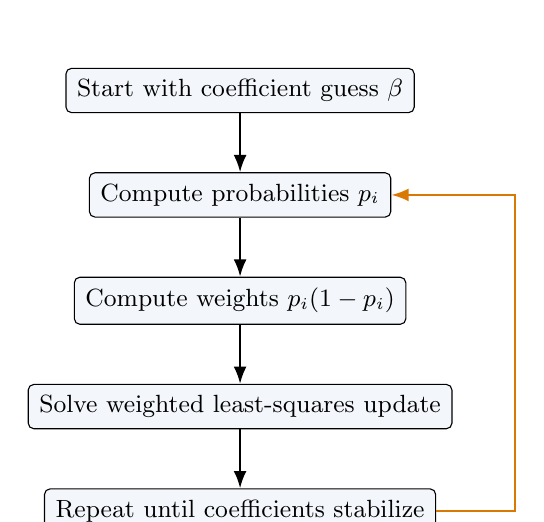
\begin{tikzpicture}[node distance=0.75cm,>=Latex]
  \node[diagramBox] (a) {Start with coefficient guess \(\beta\)};
  \node[diagramBox,below=of a] (b) {Compute probabilities \(p_i\)};
  \node[diagramBox,below=of b] (c) {Compute weights \(p_i(1-p_i)\)};
  \node[diagramBox,below=of c] (d) {Solve weighted least-squares update};
  \node[diagramBox,below=of d] (e) {Repeat until coefficients stabilize};
  \draw[diagramArrow] (a)--(b); \draw[diagramArrow] (b)--(c); \draw[diagramArrow] (c)--(d); \draw[diagramArrow] (d)--(e);
  \draw[diagramArrow,diagramOrange] (e.east) -- ++(1.0,0) |- (b.east);
\end{tikzpicture}%
}
\end{center}


\subsubsection{Odds Ratios, Log-Odds, and Marginal Effects}

A logistic coefficient is linear in log-odds, not in probability. If \(x_j\) increases by one unit while other predictors are held fixed, then
\[
\log\left(\frac{p}{1-p}\right) \text{ changes by } \beta_j.
\]
Exponentiating gives the odds-ratio interpretation:
\[
\frac{\text{new odds}}{\text{old odds}}=e^{\beta_j}.
\]
For example, if \(\beta_j=0.8\), then \(e^{0.8}\approx 2.23\). A one-unit increase in \(x_j\) multiplies the odds of class 1 by about \(2.23\), holding other predictors fixed.

The probability effect is not constant. For a continuous predictor,
\[
\frac{\partial p}{\partial x_j}=\beta_jp(1-p).
\]
This effect is largest near \(p=0.5\) and smallest when \(p\) is already close to 0 or 1. This is why the sigmoid curve is steep in the middle and flat in the tails.

\begin{center}
\small
\renewcommand{\arraystretch}{1.15}
\begin{tabular}{|L{0.22\textwidth}|L{0.30\textwidth}|L{0.36\textwidth}|}
\hline
    Quantity & Formula & Interpretation \\
\hline
    Log-odds & \(\log(p/(1-p))\) & Linear scale modeled by \(x'\beta\) \\
\hline
    Odds & \(p/(1-p)\) & Event probability relative to non-event probability \\
\hline
    Odds ratio & \(e^{\beta_j}\) & Multiplicative change in odds for one-unit increase in \(x_j\) \\
\hline
    Marginal effect & \(\beta_jp(1-p)\) & Local change in probability \\
\hline
\end{tabular}
\end{center}
\normalsize

\subsubsection{Worked Example: Credit Default Probability}

Suppose a simple logistic model for default is
\[
z=-4+0.08D,
\]
where \(D\) is debt-to-income ratio measured in percentage points. If \(D=30\), then
\[
z=-4+0.08(30)=-1.6,
\]
and
\[
p=\frac{1}{1+e^{1.6}}\approx 0.168.
\]
The predicted default probability is about \(16.8\%\). If \(D=50\), then
\[
z=-4+0.08(50)=0,
\qquad
p=0.5.
\]
Thus the model's default probability crosses the usual 0.5 decision threshold at \(D=50\). The coefficient \(0.08\) means each additional percentage point of debt-to-income multiplies default odds by
\[
e^{0.08}\approx 1.083,
\]
about an \(8.3\%\) increase in odds.

\subsubsection{Classification Metrics and Threshold Selection}

A probability model becomes a classifier only after choosing a threshold \(c\):
\[
\hat{y}=\begin{cases}
1, & \hat{p}\geq c,\\
0, & \hat{p}<c.
\end{cases}
\]
The threshold should reflect the business or scientific cost of mistakes. In fraud detection, missing fraud may be much more expensive than flagging a legitimate transaction, so \(c\) may be lower than 0.5.

\begin{center}
\small
\renewcommand{\arraystretch}{1.15}
\begin{tabular}{|L{0.22\textwidth}|L{0.30\textwidth}|L{0.36\textwidth}|}
\hline
    Metric & Formula & Best used when \\
\hline
    Accuracy & \((TP+TN)/(TP+FP+TN+FN)\) & Classes are balanced and errors have similar costs \\
\hline
    Precision & \(TP/(TP+FP)\) & False positives are costly \\
\hline
    Recall / Sensitivity & \(TP/(TP+FN)\) & False negatives are costly \\
\hline
    Specificity & \(TN/(TN+FP)\) & Correctly identifying negatives matters \\
\hline
    F1 score & \(2PR/(P+R)\) & Need one number balancing precision and recall \\
\hline
\end{tabular}
\end{center}
\normalsize

\paragraph{ROC curve and AUC.}
The ROC curve plots true positive rate against false positive rate over all possible thresholds. The area under the curve (AUC) measures ranking quality: the probability that a randomly chosen positive example receives a higher predicted score than a randomly chosen negative example.

\paragraph{Calibration.}
A model can rank cases well but still produce poorly calibrated probabilities. Calibration asks whether events predicted at probability \(0.20\) occur about \(20\%\) of the time. Log-loss and the Brier score evaluate probability quality, not just class labels:
\[
\text{Brier score}=\frac{1}{n}\sum_{i=1}^{n}(y_i-\hat{p}_i)^2.
\]

\subsubsection{Inference, Likelihood-Ratio Tests, and Separation}

Under regularity conditions, the maximum likelihood estimator is approximately normal in large samples:
\[
\hat{\beta}\approx N\left(\beta,(X'\hat{W}X)^{-1}\right).
\]
This gives Wald tests of individual coefficients:
\[
z_j=\frac{\hat{\beta}_j}{\operatorname{SE}(\hat{\beta}_j)}.
\]
For comparing nested logistic models, likelihood-ratio tests are often preferred. If \(\ell_U\) is the unrestricted log-likelihood and \(\ell_R\) is the restricted log-likelihood, then
\[
LR=2(\ell_U-\ell_R),
\]
which is approximately \(\chi^2_q\) with \(q\) restrictions under the null hypothesis.

\paragraph{Complete separation.}
If a predictor perfectly separates the classes, the likelihood is maximized by sending some coefficients toward infinity. In practice this causes huge estimates, huge standard errors, or convergence warnings. Remedies include collecting more data, simplifying predictors, or using regularization.

\paragraph{Class imbalance.}
When one class is rare, accuracy can be misleading. A fraud model that predicts ``not fraud'' for every transaction may be highly accurate but useless. Use precision, recall, AUC, calibration, class weights, resampling, or threshold tuning depending on the objective.

\subsection{Non-Linear Regression Models}


\subsubsection{Quantile Regression}


\textbf{Problem with OLS:} Linear regression models the \textbf{conditional mean} of Y. But the mean is sensitive to outliers and gives no information about the extremes of the distribution.

\textbf{Quantile regression} (Koenker \& Bassett, 1978) models the relationship between X and Y at \textbf{specific quantiles} (percentiles) of the Y distribution.

\textbf{Instead of:} "What is the average effect of X on Y?"
\textbf{It asks:} "What is the effect of X on the 10th / 50th / 90th percentile of Y?"

\textbf{Quantile regression minimizes:} Sum of \textbf{absolute} weighted errors (not squared errors):

\[
\min_\beta \sum_{i: y_i \geq \hat{y}_i} q|y_i - \hat{y}_i| + \sum_{i: y_i < \hat{y}_i} (1-q)|y_i - \hat{y}_i|
\]


Where \(q \in (0,1)\) is the quantile.

\textbf{Key advantages:}
\begin{itemize}[leftmargin=*]
    \item \textbf{Robust to outliers:} Absolute errors reduce the influence of extreme values.
    \item \textbf{Handles heteroscedasticity:} Different quantiles can have different relationships to X.
    \item \textbf{Captures extremes:} Especially useful for financial risk analysis.

\end{itemize}

\textbf{Finance example:}
\begin{itemize}[leftmargin=*]
    \item Market sentiment \(\rightarrow\) stock returns at 10th percentile (worst losses)
    \item Market sentiment \(\rightarrow\) stock returns at 90th percentile (best gains)
    \item A complete picture of risk across the return distribution, not just the average.

\end{itemize}

\medskip


\subsubsection{Decision Tree Regression}


\textbf{Concept:} Like a flowchart --- makes a series of yes/no decisions based on features to arrive at a prediction.

\textbf{Structure:}
\begin{itemize}[leftmargin=*]
    \item \textbf{Internal/Split nodes:} Where the data is divided based on a condition (e.g., "Is square footage \(>\) 1,500?")
    \item \textbf{Leaf nodes:} Terminal nodes with a prediction = average of training samples that fell into that leaf

\end{itemize}

\textbf{How it works for regression:}
\begin{enumerate}[leftmargin=*]
    \item The tree splits data into subsets based on feature thresholds.
    \item Each subset gets progressively more homogeneous.
    \item At a leaf, the prediction = mean (or median) of Y values of all training points in that leaf.
    \item This creates a step-function prediction surface (not a smooth line).

\end{enumerate}

\textbf{Example --- predicting quarterly sales revenue:}

\begin{center}
\resizebox{0.95\textwidth}{!}{%
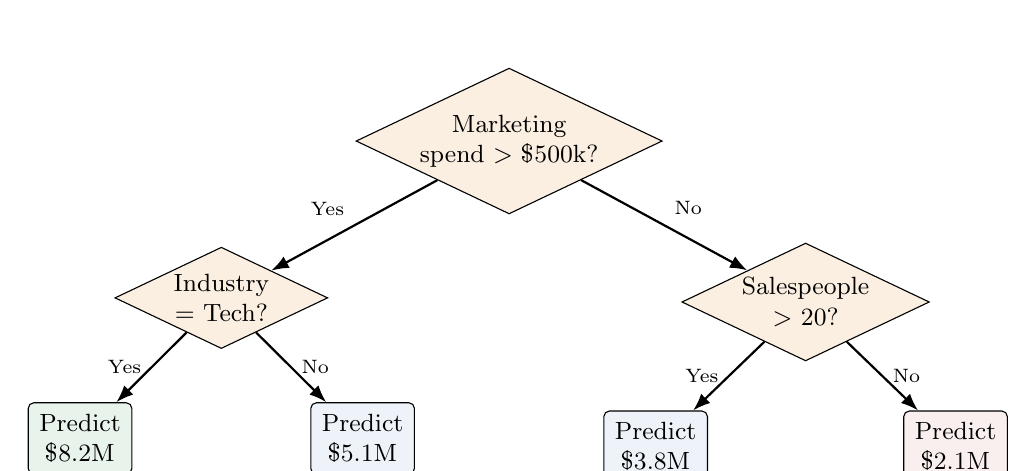
\begin{tikzpicture}[node distance=1.0cm and 1.1cm,>=Latex]
  \node[diagramDecision] (root) {Marketing\\spend \(>\) \$500k?};
  \node[diagramDecision,below left=1.2cm and 2.0cm of root] (tech) {Industry\\= Tech?};
  \node[diagramDecision,below right=1.2cm and 2.0cm of root] (sales) {Salespeople\\\(>\) 20?};
  \node[diagramBox,fill=diagramGreen!10,below left=1.0cm and 0.45cm of tech] (a) {Predict\\\$8.2M};
  \node[diagramBox,fill=diagramBlue!8,below right=1.0cm and 0.45cm of tech] (b) {Predict\\\$5.1M};
  \node[diagramBox,fill=diagramBlue!8,below left=1.0cm and 0.45cm of sales] (c) {Predict\\\$3.8M};
  \node[diagramBox,fill=bearc!8,below right=1.0cm and 0.45cm of sales] (d) {Predict\\\$2.1M};
  \draw[diagramArrow] (root) -- node[above left,font=\scriptsize]{Yes} (tech);
  \draw[diagramArrow] (root) -- node[above right,font=\scriptsize]{No} (sales);
  \draw[diagramArrow] (tech) -- node[left,font=\scriptsize]{Yes} (a);
  \draw[diagramArrow] (tech) -- node[right,font=\scriptsize]{No} (b);
  \draw[diagramArrow] (sales) -- node[left,font=\scriptsize]{Yes} (c);
  \draw[diagramArrow] (sales) -- node[right,font=\scriptsize]{No} (d);
\end{tikzpicture}%
}
\end{center}



\textbf{Caution:}
\begin{itemize}[leftmargin=*]
    \item \textbf{Overfitting:} Trees can grow very deep, memorizing training data.
    \item \textbf{Instability:} Small changes in data \(\rightarrow\) very different tree structures.

\end{itemize}

\medskip


\subsubsection{Random Forest Regression}


\textbf{Core idea:} Instead of one decision tree, build \textbf{hundreds of trees} and average their predictions. The "wisdom of the crowd" principle.

\textbf{Two sources of "randomness":}

\begin{enumerate}[leftmargin=*]
    \item \textbf{Random data subsets (Bootstrapping):} Each tree is trained on a random sample of the training data (with replacement). Some data points may be selected multiple times; others may be left out for that specific tree.

    \item \textbf{Random feature subsets:} At each split, only a random subset of features is considered (not all features). This forces trees to be different from each other.

\end{enumerate}

\textbf{Making predictions:}
\[
\hat{y} = \frac{1}{T}\sum_{t=1}^{T}\hat{y}_t
\]


The final prediction is the \textbf{average} of all T individual tree predictions.

\textbf{Advantages over single decision trees:}
\begin{itemize}[leftmargin=*]
    \item Much lower variance (averaging smooths out individual tree instability)
    \item Less prone to overfitting
    \item Naturally handles non-linear relationships
    \item Provides \textbf{feature importance scores} (how much each feature contributes)

\end{itemize}

\textbf{Trade-offs:}
\begin{itemize}[leftmargin=*]
    \item \textbf{Black box:} Hard to interpret why a specific prediction was made
    \item \textbf{Computationally intensive:} Training hundreds of trees requires more time and memory

\end{itemize}

\textbf{Finance example --- predicting stock volatility:}
\begin{itemize}[leftmargin=*]
    \item Features: recent volatility, trading volume, VIX index
    \item Single tree: unstable, overfits historical patterns
    \item Random forest: builds 500 trees, each on different data samples \(\rightarrow\) final prediction = average of 500 estimates \(\rightarrow\) more stable, reliable volatility forecast

\end{itemize}

\medskip


\subsubsection{Support Vector Regression (SVR)}


\textbf{Core concept:} Find a function that fits within an \(\varepsilon\)-wide "tube" around the regression line. Points inside the tube are considered "good enough" --- no penalty. Only points outside the tube incur loss.

\textbf{The \(\varepsilon\)-Insensitive Tube:}


\begin{center}
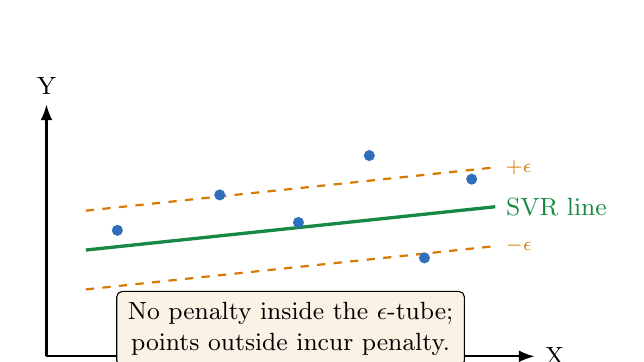
\begin{tikzpicture}[x=1cm,y=1cm,>=Latex]
  \draw[diagramAxis] (0,0) -- (6.2,0) node[right,font=\small]{X};
  \draw[diagramAxis] (0,0) -- (0,3.2) node[above,font=\small]{Y};
  \draw[diagramGreen,very thick] (0.5,1.35) -- (5.7,1.9) node[right,font=\small]{SVR line};
  \draw[diagramOrange,thick,dashed] (0.5,1.85) -- (5.7,2.4) node[right,font=\scriptsize]{\(+\epsilon\)};
  \draw[diagramOrange,thick,dashed] (0.5,0.85) -- (5.7,1.4) node[right,font=\scriptsize]{\(-\epsilon\)};
  \foreach \x/\y in {0.9/1.6,1.6/0.7,2.2/2.05,3.2/1.7,4.1/2.55,4.8/1.25,5.4/2.25}{\fill[diagramBlue] (\x,\y) circle (2pt);}
  \node[diagramBox,fill=diagramOrange!10] at (3.1,0.35) {No penalty inside the \(\epsilon\)-tube;\\points outside incur penalty.};
\end{tikzpicture}
\end{center}



\textbf{SVR formulation:}
\[
\min \frac{1}{2}\|w\|^2 + C\sum_{i}(\xi_i + \xi_i^*)
\]


Subject to:
\begin{itemize}[leftmargin=*]
    \item \(y_i - (w \cdot x_i + b) \leq \varepsilon + \xi_i\)
    \item \((w \cdot x_i + b) - y_i \leq \varepsilon + \xi_i^*\)

\end{itemize}

Where \(\xi, \xi^*\) are slack variables for points outside the tube, and \(C\) controls the penalty for those points.

\textbf{The Kernel Trick:} For non-linear relationships, SVR maps data to a higher-dimensional space where it may be linearly separable:

\begin{center}
\small
\renewcommand{\arraystretch}{1.15}
\begin{tabular}{|L{0.28\textwidth}|L{0.60\textwidth}|}
\hline
    Kernel & Use Case \\
\hline
    \textbf{Linear} & Linearly separable data \\
\hline
    \textbf{Polynomial} & Moderate non-linearity \\
\hline
    \textbf{RBF (Radial Basis Function)} & Complex, highly non-linear patterns \\
\hline
\end{tabular}
\end{center}
\normalsize


\textbf{Finance example --- option pricing:}
\begin{itemize}[leftmargin=*]
    \item Input features: underlying stock price, time to expiry, implied volatility, interest rates
    \item These have complex, non-linear interactions
    \item SVR with RBF kernel can capture these relationships
    \item The \(\varepsilon\)-tube tolerates small pricing errors (e.g., within \(\pm\)\$0.05) without penalty

\end{itemize}

\medskip


\subsection{Comprehensive Summary}


\subsubsection{Choosing the Right Regression Model}



\begin{center}
\resizebox{\textwidth}{!}{%
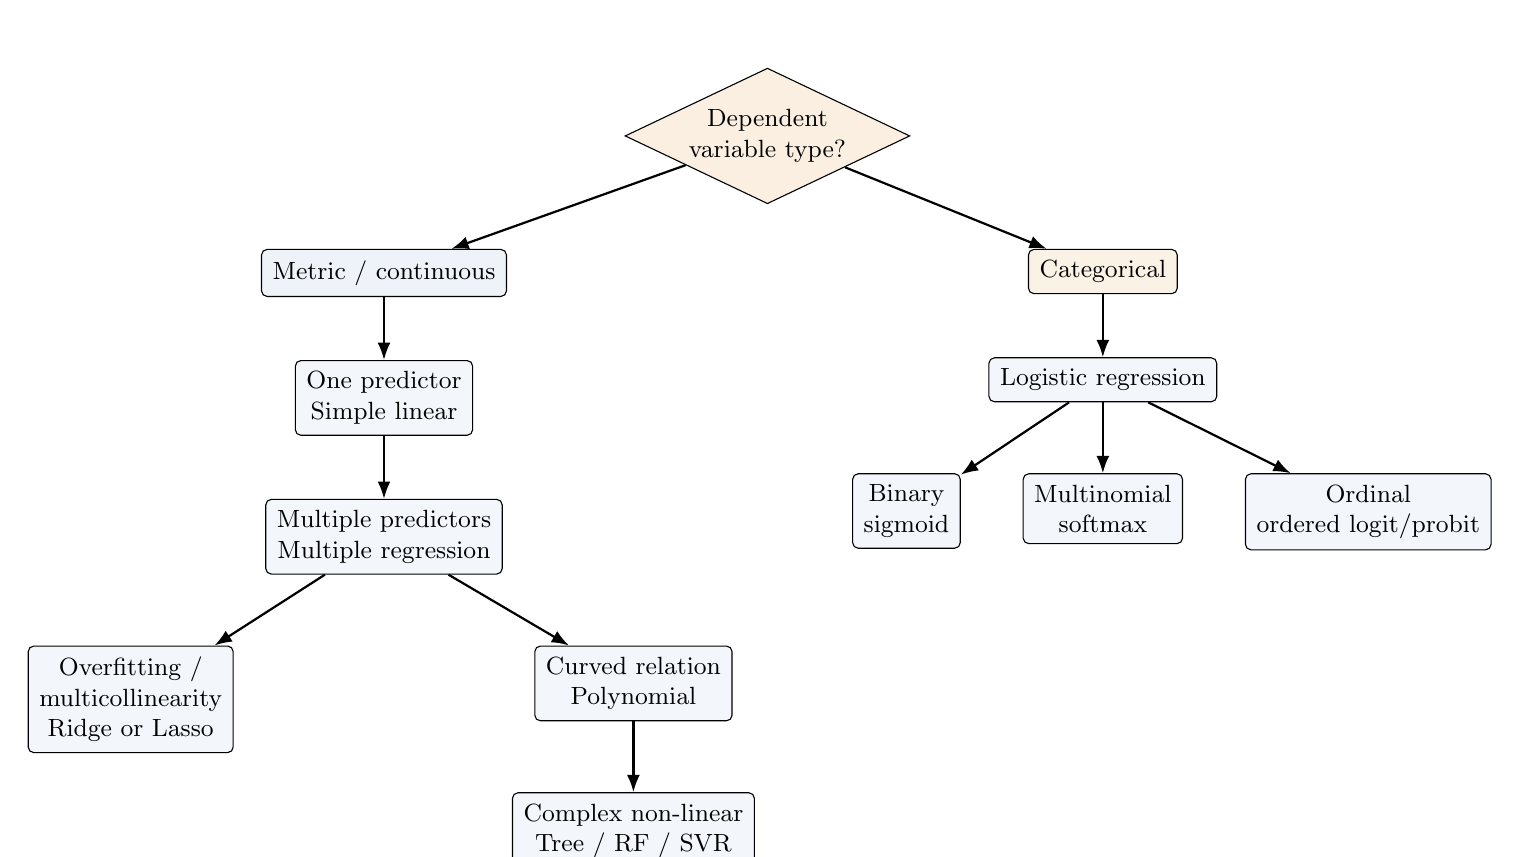
\begin{tikzpicture}[node distance=0.8cm and 0.85cm,>=Latex]
  \node[diagramDecision] (root) {Dependent\\variable type?};
  \node[diagramBox,fill=diagramBlue!8,below left=1.0cm and 2.4cm of root] (metric) {Metric / continuous};
  \node[diagramBox,fill=diagramOrange!10,below right=1.0cm and 2.4cm of root] (cat) {Categorical};
  \node[diagramBox,below=of metric] (one) {One predictor\\Simple linear};
  \node[diagramBox,below=of one] (many) {Multiple predictors\\Multiple regression};
  \node[diagramBox,below left=0.9cm and 0.4cm of many] (ridge) {Overfitting /\\multicollinearity\\Ridge or Lasso};
  \node[diagramBox,below right=0.9cm and 0.4cm of many] (poly) {Curved relation\\Polynomial};
  \node[diagramBox,below=0.9cm of poly] (tree) {Complex non-linear\\Tree / RF / SVR};
  \node[diagramBox,below=of cat] (logit) {Logistic regression};
  \node[diagramBox,below left=0.9cm and 0.35cm of logit] (binary) {Binary\\sigmoid};
  \node[diagramBox,below=0.9cm of logit] (multi) {Multinomial\\softmax};
  \node[diagramBox,below right=0.9cm and 0.35cm of logit] (ordinal) {Ordinal\\ordered logit/probit};
  \draw[diagramArrow] (root)--(metric); \draw[diagramArrow] (root)--(cat);
  \draw[diagramArrow] (metric)--(one); \draw[diagramArrow] (one)--(many); \draw[diagramArrow] (many)--(ridge); \draw[diagramArrow] (many)--(poly); \draw[diagramArrow] (poly)--(tree);
  \draw[diagramArrow] (cat)--(logit); \draw[diagramArrow] (logit)--(binary); \draw[diagramArrow] (logit)--(multi); \draw[diagramArrow] (logit)--(ordinal);
\end{tikzpicture}%
}
\end{center}


\section{Decision Trees}

Decision trees are a type of \textbf{supervised learning algorithm} used for both \textbf{classification} and \textbf{regression} tasks. They work by recursively splitting a dataset into subsets based on feature values, producing a tree-like structure where:

\begin{itemize}[leftmargin=*]
    \item Each \textbf{internal (decision) node} represents a decision rule (a test/condition) on one attribute.
    \item Each \textbf{leaf (terminal) node} corresponds to a final class label (classification) or a numerical prediction (regression).

\end{itemize}

In finance and trading, decision trees help model complex, non-linear relationships between market indicators (moving averages, volume, technical ratios, etc.) and target outcomes ("buy" vs. "sell", future price direction, expected returns, etc.). Their hierarchical, rule-based structure makes them \textbf{highly interpretable} --- a trader or analyst can trace the exact path of conditions that led to a prediction --- while still capturing patterns that simple linear models cannot.

\begin{quote}
\textbf{Note:} Decision trees are among the most interpretable ML models and form the foundation of advanced ensemble techniques such as \textbf{Random Forests} and \textbf{Gradient Boosting}, which are widely used in quantitative finance and algorithmic trading.
\end{quote}


\medskip


\subsection{Core Concepts and Terminology}


\subsubsection{Classification Trees vs. Regression Trees}

Decision trees (collectively called \textbf{CART} --- Classification And Regression Trees) come in two flavors, which share the same tree structure but differ in their objective:

\begin{center}
\small
\renewcommand{\arraystretch}{1.15}
\begin{tabular}{|L{0.24\textwidth}|L{0.26\textwidth}|L{0.38\textwidth}|}
\hline
    Type & Output & Example \\
\hline
    \textbf{Classification Tree} & Categorical variable & Will the market go \textbf{up or down} tomorrow? Yes/No, Red/Blue/Yellow \\
\hline
    \textbf{Regression Tree} & Continuous numeric variable & What will \textbf{tomorrow's return} be? \\
\hline
\end{tabular}
\end{center}
\normalsize


\begin{quote}
\textbf{Warning:} A regression \textit{tree} should not be confused with \textbf{linear regression}. Linear regression studies the relationship between variables using a single equation; a regression tree partitions the data into regions and predicts a constant (usually the average) value within each region.
\end{quote}


\subsubsection{Tree Structure}

Every decision tree --- classification or regression --- has the same anatomy:

\begin{itemize}[leftmargin=*]
    \item \textbf{Root Node}: The very top of the tree. It contains the entire dataset and has \textbf{no incoming pathway}, only outgoing ones.
    \item \textbf{Internal Nodes} (a.k.a. \textbf{decision nodes}, \textbf{branches}, or \textbf{test nodes}): Located in the middle levels. They contain a splitting condition and have \textbf{both incoming and outgoing pathways}.
    \item \textbf{Leaf Nodes} (a.k.a. \textbf{decision nodes/terminal nodes}): At the bottom of the tree. They have an \textbf{incoming pathway but no outgoing pathway}, and they hold the final output (a class label or a numeric prediction).
\end{itemize}


\subsubsection{How a Tree Is Used to Classify/Predict}

A decision tree makes a statement (a condition) at each node and moves down a branch depending on whether that statement is \textbf{true or false}:

\begin{itemize}[leftmargin=*]
    \item By convention, if a node's statement is \textbf{true}, you move to the \textbf{left} child; if \textbf{false}, you move to the \textbf{right} child (though trees are sometimes drawn with explicit True/False labels on the edges instead).
    \item You start at the root and keep testing conditions, moving down the tree until you reach a leaf --- at which point that leaf's value is the prediction.
    \item Because trees are drawn as a series of nested conditions, at a glance a decision tree is really just a structured set of \textbf{nested if-else statements}. What makes it "machine learning" is that the algorithm \textit{learns} which features and which threshold values to use at each split, rather than a human hard-coding them.
    \item A tree can \textbf{mix data types} freely (numeric thresholds and yes/no conditions in the same tree), and the same feature can be tested \textbf{more than once} at different nodes, potentially with different thresholds each time.
    \item Multiple leaves can end up with the \textbf{same output class} --- there's no requirement that every leaf be unique.
\end{itemize}


\subsubsection{Pure vs. Impure Nodes}

\begin{itemize}[leftmargin=*]
    \item A node/leaf is \textbf{pure} if it contains observations from only \textbf{one class} (e.g., a leaf where every single data point loves popcorn belongs to the same "cool as ice" outcome).
    \item A node/leaf is \textbf{impure} if it contains a \textbf{mixture} of classes.
    \item The entire tree-building process is about choosing splits that make the resulting child nodes as pure as possible.
\end{itemize}


\medskip


\subsection{Building a Decision Tree: Splitting Criteria}


To build a tree "from scratch," the algorithm must decide, at every node, \textbf{which feature to split on} and \textbf{at what threshold}. This is done by testing candidate splits and picking the one that produces the \textbf{least impurity} (equivalently, the \textbf{most information gain}) in the resulting child nodes. This is done recursively until a stopping condition is reached (e.g., nodes become pure, or a limit like max depth/min samples is hit).

There are two dominant impurity measures: \textbf{Gini Impurity} and \textbf{Entropy / Information Gain}. Numerically they behave very similarly, but their formulas differ.

\subsubsection{Gini Impurity}


\textbf{Formula (per node):}

\[
\text{Gini} = 1 - \sum_i p_i^2
\]


For a binary classification leaf with classes "Yes" and "No":

\[
\text{Gini} = 1 - (p_{\text{yes}})^2 - (p_{\text{no}})^2
\]


where \(p_{\text{yes}}\) and \(p_{\text{no}}\) are the proportions of "Yes" and "No" observations that land in that leaf.

\textbf{Worked example} (from the "loves popcorn / loves soda / age \(\rightarrow\) loves \textit{Cool as Ice}" dataset):

\begin{itemize}[leftmargin=*]
    \item \textbf{Leaf on the left of the "Loves Popcorn" split} has 4 people, of whom 1 loves \textit{Cool as Ice} and 3 do not:
\end{itemize}

\[
\text{Gini}_{\text{left}} = 1 - \left(\frac{1}{4}\right)^2 - \left(\frac{3}{4}\right)^2 = 0.375
\]

\begin{itemize}[leftmargin=*]
    \item \textbf{Leaf on the right} (3 people) works out to:
\end{itemize}

\[
\text{Gini}_{\text{right}} = 0.444
\]


\textbf{Weighted (total) Gini Impurity for a split:} Because the two leaves usually don't contain the same number of observations, the overall impurity of a split is the \textbf{weighted average} of the leaf impurities, weighted by the number of samples in each leaf:

\[
\text{Gini}_{\text{split}} = \frac{n_{\text{left}}}{N}\cdot \text{Gini}_{\text{left}} + \frac{n_{\text{right}}}{N}\cdot \text{Gini}_{\text{right}}
\]


For the popcorn example (4 people left, 3 people right, 7 total):

\[
\text{Gini}_{\text{popcorn}} = \frac{4}{7}(0.375) + \frac{3}{7}(0.444) = 0.405
\]


Doing the same calculation for "Loves Soda" gives \textbf{Gini = 0.214} --- lower than popcorn's 0.405, meaning a split on "loves soda" produces purer children than a split on "loves popcorn."

\textbf{Handling numeric features (e.g., Age):}

Numeric predictors need an extra step because there's no natural "category" to split on. The procedure is:

\begin{enumerate}[leftmargin=*]
    \item \textbf{Sort} all observations by the numeric feature (ascending).
    \item Compute the \textbf{average of every pair of adjacent values} --- these averages become the \textbf{candidate thresholds} (e.g., if two adjacent ages are 9 and 10, the candidate threshold is 9.5).
    \item For each candidate threshold, build a simple split ("age \(<\) threshold" vs. "age \(\geq\) threshold") and compute the weighted Gini impurity exactly as above.
    \item Pick the threshold that gives the \textbf{lowest} Gini impurity.

\end{enumerate}

In the worked example, thresholds of \textbf{15} and \textbf{44} were tied for the lowest impurity (0.343), and 15 was arbitrarily chosen.

\textbf{Choosing the root (and every subsequent split):}
Compare the best Gini score achievable from each candidate feature (popcorn = 0.405, soda = 0.214, age = 0.343). The feature with the \textbf{lowest impurity} wins that node. In this example, "Loves Soda" had the lowest score, so it became the \textbf{root node}.

\textbf{Recursive splitting:} After the root split, look at each resulting child node. If a child is impure, repeat the entire process (comparing candidate splits on the \textit{remaining} features, using only the subset of data that reached that node) to decide whether and how to split it further. If a split doesn't reduce impurity below what's already there, or if there's no reason to split further (e.g., you've isolated a small group), that node becomes a \textbf{leaf}.

\textit{Example continuation:} Among people who love soda, splitting further on "loves popcorn" gave a weighted Gini of 0.25, while splitting on "age \(<\) 12.5" gave a weighted Gini of 0.0 (both children pure). Since 0 \(<\) 0.25, the age split was chosen for that branch.

\textbf{Assigning leaf outputs:} Once a leaf is finalized (pure or not), its predicted output is simply \textbf{whichever class is the majority} among the samples that landed there (majority voting). Even an impure leaf must output a single class --- it uses the majority class, and the leaf's purity level (e.g., "75\% of samples here love Cool as Ice") gives a sense of the confidence/accuracy of that prediction.

\textbf{Making a prediction for new data:} Run the new observation down the tree, testing each condition until it reaches a leaf, and output that leaf's majority class.

\subsubsection{Entropy and Information Gain}


An alternative (and very popular) impurity measure is \textbf{entropy}, borrowed from information theory. It measures the amount of "uncertainty" or "disorder" in a state.

\textbf{Formula:}

\[
H = -\sum_i p_i \log_2(p_i)
\]


\begin{itemize}[leftmargin=*]
    \item If a node has a \textbf{50/50} split between two classes, entropy is at its \textbf{maximum value of 1} --- maximum uncertainty, since a randomly picked point is a coin flip.
    \item If a node is \textbf{pure} (all one class), entropy is \textbf{0} --- no uncertainty at all.

\end{itemize}

\textbf{Information Gain} for a candidate split is the \textit{reduction} in entropy achieved by splitting the parent node into children:

\[
\text{Information Gain} = H_{\text{parent}} - \sum_{\text{children}} \left(\frac{n_{\text{child}}}{N_{\text{parent}}}\right) H_{\text{child}}
\]


Just like with Gini, the child entropies are weighted by the relative size (proportion of samples) of each child node relative to the parent.

\textbf{Decision rule:} At every node, the algorithm evaluates \textit{every possible feature and every possible threshold value}, computes the information gain for each candidate split, and selects the split that \textbf{maximizes information gain} (equivalently, minimizes weighted child entropy). This is repeated recursively at each new node until the tree is fully grown.

\textbf{Example intuition (2D feature space, x0 and x1):}
Given two candidate splits --- (a) "x1 \(\leq\) 4" and (b) "x0 \(\leq\) -12" --- you compute the information gain for both. The split that produces a \textbf{purer child} (e.g., one child containing only "red" points) yields \textbf{higher information gain} and is chosen. In practice the model doesn't just compare two candidates; it exhaustively searches over all features and all thresholds.

\subsubsection{The Greedy Nature of Decision Trees}


A crucial property: \textbf{decision trees are greedy algorithms}. At each node, the algorithm picks the split that is locally optimal (maximizes information gain / minimizes impurity \textit{at that step}) --- it does \textbf{not} look ahead or backtrack to reconsider earlier splits based on how later splits turn out.

\begin{itemize}[leftmargin=*]
    \item \textbf{Consequence:} greedy search does not guarantee the globally optimal tree structure overall.
    \item \textbf{Benefit:} it makes training dramatically faster and, despite the theoretical suboptimality, works very well in practice.
\end{itemize}


\subsubsection{Visualizing a Trained Tree (General Principles)}


When a tree is visualized (e.g., via \texttt{graphviz}), each node typically displays:

\begin{itemize}[leftmargin=*]
    \item The \textbf{predictor variable and threshold} used to split the data at that node.
    \item The node's \textbf{impurity value}: Gini for classification or MSE for regression.
    \item The \textbf{number of samples} that reached that node.
    \item The \textbf{class counts} (for classification) belonging to each output category.

\end{itemize}

By reading pure (or near-pure) leaves, you can often "read off" \textbf{human-interpretable rules}, e.g., \textit{"if ADX \(\leq\) 19.24 and RSI is between 62.55 and 62.95, the market tends to go up."} This interpretability is one of the biggest advantages of decision trees over black-box models.

\medskip


\subsection{Overfitting and Pruning}


\subsubsection{The Overfitting Problem}

If a tree is allowed to grow without limit, it will keep splitting until leaves are perfectly pure --- sometimes down to a \textbf{single observation} per leaf. A leaf built from just one data point gives no real statistical confidence that it will generalize to new, unseen data. This is a classic case of \textbf{overfitting}: the tree has essentially memorized the training data's noise rather than learning a generalizable pattern.

\subsubsection{Solutions}

\begin{enumerate}[leftmargin=*]
    \item \textbf{Constrain tree growth (pre-pruning / early stopping):} Set limits \textit{during} the tree-building process, such as:
\end{enumerate}

\begin{itemize}[leftmargin=*]
    \item \textbf{Maximum depth} the tree is allowed to reach.
    \item \textbf{Minimum number of samples required per leaf} (e.g., require at least 3, 6, or 200 samples per leaf, depending on dataset size).

This trades off perfect purity for leaves that are statistically more reliable (even if impure), while also giving a built-in sense of prediction confidence (e.g., "75\% of the samples in this leaf belong to the majority class").

\end{itemize}

\begin{enumerate}[leftmargin=*]
    \item \textbf{Pruning (post-pruning):} Grow the tree fully first, and then \textbf{remove branches} that don't meaningfully improve predictive performance, typically evaluated against a separate \textbf{validation dataset}.

\end{enumerate}

Since the "right" value for a constraint like minimum samples per leaf isn't known in advance, it is common to test several candidate values using \textbf{cross-validation} and pick whichever performs best on held-out data.

\subsubsection{Pruning in a Financial Context}

\begin{itemize}[leftmargin=*]
    \item \textbf{Pre-pruning (early stopping):} Set constraints such as maximum tree depth or a minimum number of data points required to make a split, preventing the model from growing excessively large in the first place.
    \item \textbf{Post-pruning:} Grow the tree fully, then systematically remove branches that don't add substantial predictive value, using validation data to decide what to cut. Growing the tree out fully (before this pruning is applied) is the stage where the model is at greatest risk of having overfit the training data --- pruning afterward is what corrects for that.

\end{itemize}

Pruning generally makes the resulting tree \textbf{more streamlined} and better at generalizing to real-world, out-of-sample scenarios --- which is especially important in finance, where overfit models can look excellent on historical (backtested) data yet fail live.

\medskip


\subsection{Decision Trees in Finance}


Decision trees are a major tool in corporate finance, economics, and decision analysis --- used to visualize financial choices, the risks attached to them, and their possible outcomes.

\subsubsection{Basic Structure in a Financial Decision Tree}

\begin{itemize}[leftmargin=*]
    \item \textbf{Decision nodes:} Represent a big decision point, such as choosing to undertake a capital project or choosing between competing ventures.
    \item \textbf{End/outcome nodes:} Represent a speculative projected outcome of a course of action (e.g., "earnings are expected to increase by \$5 million").
    \item \textbf{Chance nodes:} Attach a \textbf{probability} to a specific projected outcome actually occurring, since outcomes are inherently uncertain/speculative.

\end{itemize}

As decisions become more complex (many contingent, cascading outcomes), simple historical-frequency probability estimates aren't enough, and \textbf{Bayesian probability models} are used to derive the necessary \textit{priori} (prior) probabilities.

\subsubsection{Binomial Option Pricing}


Decision tree analysis is commonly applied to \textbf{option pricing} via the \textbf{binomial option pricing model}, which uses discrete probabilities to determine an option's value at expiration.

\begin{itemize}[leftmargin=*]
    \item \textbf{Basic (European) case:} The simplest binomial models assume the underlying asset's value will either \textbf{rise or fall}, each with some calculated probability, by the option's maturity date.
    \item \textbf{American options (more complex):} Because American options can be exercised \textbf{at any point up to maturity} (not just at expiration), the binomial tree must factor in \textbf{multiple possible price paths} the underlying asset can take over time --- not just a single up/down step.
    \item \textbf{Convergence to Black-Scholes:} As the number of nodes (time steps) in the binomial tree increases toward infinity, the binomial model's output \textbf{converges to the Black-Scholes formula}.
    \item \textbf{Why still use binomial trees if Black-Scholes exists?} Black-Scholes is computationally simpler, but computer software can build binomial trees with effectively "infinite" nodes, which can produce \textbf{more accurate pricing}, especially for:
    \item \textbf{Bermuda options} (exercisable only at specific pre-set dates, a middle ground between European and American style).
    \item \textbf{Dividend-paying stocks} (where cash payouts complicate the closed-form Black-Scholes assumptions).
\end{itemize}


\subsubsection{Real Option Analysis}


\textbf{Real options} are actual strategic decisions a company can make partway through a project --- such as an \textbf{expansion option} or an \textbf{abandonment option}. Unlike financial options, their value \textbf{cannot} be determined using the Black-Scholes formula, and must instead be valued using decision trees.

\textbf{Example (oil \& gas company):}
\begin{enumerate}[leftmargin=*]
    \item The company purchases a piece of land today (this is like buying the "option").
    \item It drills exploratory wells.
    \item \textbf{If drilling is successful}, the company can then cheaply purchase \textit{additional} adjacent lots of land (exercising the real option to expand).
    \item \textbf{If drilling is unsuccessful}, the company simply does not exercise the option --- it expires worthless, and the company's loss is capped at the cost of the original land/drilling.

\end{enumerate}

Because this optionality has real value, real options are an important part of \textbf{capital budgeting}. In fact, once the probabilities of success/failure are properly incorporated via a decision tree, a project's expected value can shift: companies often initially reject projects that look like they have a \textbf{negative Net Present Value (NPV)} under a naive analysis, but once the value of the embedded real option is accounted for, the \textbf{true NPV becomes positive}.

\subsubsection{Corporate / Project Decision Analysis}


Companies constantly face decisions around product development, staffing, operations, and mergers \& acquisitions (M\&A). Decision trees let a company \textbf{systematically and simultaneously evaluate multiple alternatives} side-by-side.

\begin{itemize}[leftmargin=*]
    \item \textbf{Example:} A decision tree can estimate the expected financial impact of hiring an employee who ultimately fails to meet expectations and must be terminated --- weighing the probability-adjusted costs against the probability-adjusted benefits of hiring.
    \item \textbf{Example (marketing):} Before airing a multimillion-dollar Super Bowl commercial, a firm can map out the different possible outcomes of the campaign, factoring in variables such as: the appeal of the commercial itself, the broader economic outlook, product quality, and competitors' advertising. Once each variable's impact and probability are estimated, the decision tree formally supports the "run the ad or not" decision.

\end{itemize}

\begin{quote}
Decision trees aren't meant for \textit{every} small/micro decision a business makes --- but they provide a useful general framework for major decisions and for managing the downstream consequences of those decisions.
\end{quote}


\subsubsection{Pricing Interest Rate Instruments with Binomial Trees}


Although technically distinct from a "decision tree" (there's no explicit choice being made --- it models an \textit{uncertain variable}, not a decision), a \textbf{binomial tree} is built the same way and serves a similar purpose: modeling the impact of a fluctuating/uncertain variable over time.

\begin{itemize}[leftmargin=*]
    \item Interest rate movements (up/down) significantly affect the prices of \textbf{fixed income securities} and \textbf{interest rate derivatives}.
    \item Binomial trees let investors accurately value bonds that have \textbf{embedded call and put provisions}, by modeling uncertain future interest-rate paths.
    \item \textbf{Why not Black-Scholes here?} The Black-Scholes model is not applicable to valuing bonds or interest-rate-based options, making the binomial model the standard alternative.
    \item Corporate projects, as well as \textbf{interest rate floors, caps, swaps}, and other rate-sensitive instruments, are commonly valued this way --- by analyzing outcomes across different possible interest-rate environments.
\end{itemize}


\subsubsection{Limitations of Decision Trees in Finance}


\begin{enumerate}[leftmargin=*]
    \item \textbf{Curse of dimensionality:} As the number of variables and possible outcomes grows, the tree can become extremely complex --- too much branching information can make the decision harder to parse rather than easier (illustrated by the multi-factor "Corporate Analysis"/Super Bowl ad example).

    \item \textbf{Reliance on subjective probability estimates:} Many financial scenarios (predicting market direction, estimating default risk) require assigning probabilities from historical data or expert judgment. These estimates may not be reliable --- for instance, the historical causes of past recessions don't necessarily tell you the true probability of a \textit{future} recession.

    \item \textbf{Struggles with correlated variables:} Financial variables are frequently interdependent (e.g., interest rates, inflation, and stock prices all influence one another). Standard decision trees do \textbf{not} inherently model these interdependencies, which can lead to \textbf{oversimplified conclusions}.

    \item \textbf{Poor fit for continuous/non-linear data:} Financial markets often show complex, continuous, non-linear patterns that are better captured by more advanced statistical or machine learning methods, such as \textbf{neural networks}. Example: credit risk assessment often involves too many interrelated variables for a simple tree structure to model well.

\end{enumerate}

\begin{quote}
\textbf{Fast Fact:} Decision trees work well for \textbf{structured} financial decisions; neural networks tend to be better suited for \textbf{pattern recognition and forecasting} in noisier, more continuous domains.
\end{quote}


\subsubsection{Popular Software for Decision Tree Analysis in Finance}


\begin{center}
\small
\renewcommand{\arraystretch}{1.15}
\begin{tabular}{|L{0.30\textwidth}|L{0.58\textwidth}|}
\hline
    Tool & Notes \\
\hline
    \textbf{Microsoft Excel} & Most widely used for \textit{basic} decision tree modeling; can be built manually with built-in functions, or with add-ins like \textbf{XLMiner} for more advanced analysis. \\
\hline
    \textbf{R} & The \textbf{\texttt{rpart}} package supports building, pruning, and optimizing decision trees using ML techniques; R generally handles larger datasets and more complex calculations well. \\
\hline
    \textbf{Python (Scikit-learn)} & Implements decision tree classifiers and regressors; integrates easily with other financial modeling tools/pipelines. \\
\hline
    \textbf{Specialized platforms} (Palantir, SAS, MATLAB) & Suited for institutions that need robust analysis where decision-tree-style modeling is core to the business (e.g., underwriting, corporate analytics). \\
\hline
\end{tabular}
\end{center}
\normalsize


\subsubsection{Quick-Reference Q\&A (Finance Context)}


\begin{itemize}[leftmargin=*]
    \item \textbf{What is a decision tree in finance?} A graphical representation of the possible choices, outcomes, and risks involved in a financial decision --- combining decision nodes, chance events, and outcome nodes to help analysts visualize scenarios and optimize decisions.
    \item \textbf{How are decision trees used in investment analysis?} They help investors map the risks and rewards of different investment opportunities; by assigning probabilities and expected values to outcomes, investors can compare options by expected return \textbf{and} by downside/potential-loss exposure.
    \item \textbf{How are probabilities assigned?} From historical data, expert judgment, or statistical models. Since probabilities drive the entire tree's output, analysts typically spend most of their effort estimating these chances accurately (e.g., "a 40\% chance of recession").
    \item \textbf{What is Expected Value (EV) in a decision tree?} The \textbf{weighted average of all possible outcomes}, weighted by their respective probabilities. It lets decision-makers compare alternative choices and select the one with the highest EV.
\end{itemize}


\medskip


\subsection{Building a Decision Tree for Trading in Python}


This section walks through a practical, end-to-end example: building both a \textbf{classification tree} (predict up/down) and a \textbf{regression tree} (predict the actual next-day return) on market data.

\subsubsection{Environment / Libraries Needed}

\begin{itemize}[leftmargin=*]
    \item \textbf{Python 3.6}
    \item \textbf{Pandas} --- data structures/handling
    \item \textbf{NumPy} --- numerical/scientific functions
    \item \textbf{Quandl} --- market data retrieval
    \item \textbf{TA-Lib} --- technical indicator calculations
    \item \textbf{Scikit-learn (\texttt{sklearn})} --- building and evaluating the trees
    \item \textbf{Graphviz} --- visualizing the trained tree
\end{itemize}


\subsubsection{The Six-Step Workflow}

\begin{enumerate}[leftmargin=*]
    \item Retrieve market data for a financial instrument.
    \item Define \textbf{predictor variables} (technical indicators, sentiment indicators, breadth indicators, etc.).
    \item Define the \textbf{target variable} (the desired output).
    \item Split the data into \textbf{training} and \textbf{test} sets.
    \item \textbf{Train} (fit) the decision tree model.
    \item \textbf{Test and analyze} the model's performance.

\end{enumerate}

Steps 1--4 are standard data-processing/backtesting steps common to \textit{any} ML or rule-based strategy (you always need a held-out test set to avoid evaluating a model on data it has already seen). Steps 5--6 are specific to the tree algorithm itself.

\subsubsection{Getting the Data}


Financial time series typically include Open, High, Low, Close (Settle), and Volume, recorded at some frequency (minute/hour/day/week). Common free data sources include the Quandl API, Yahoo Finance, and Google Finance.

Example --- retrieving \textasciitilde{}21 years of daily Emini S\&P 500 futures data via Quandl:

\begin{Verbatim}[breaklines=true,fontsize=\small]
import quandl
df = quandl.get("CHRIS/CME_ES2")
df.head()
df.tail()
df.shape   # (5391, 8) -> just over 21 years of data
\end{Verbatim}


The \textbf{Settle price} is used as the closing price reference for this instrument.

\subsubsection{Creating the Predictor Variables}


Predictors are any data believed to relate to future market behavior: technical indicators, market/sentiment/breadth data, fundamental data, government data, etc. Here, classic \textbf{trend-following} and \textbf{range-trading} indicators are used:

\begin{itemize}[leftmargin=*]
    \item \textbf{EMA} (Exponential Moving Average) --- 10-period and 30-period
    \item \textbf{ATR} (Average True Range, 14-period)
    \item \textbf{ADX} (Average Directional Index, 14-period)
    \item \textbf{RSI} (Relative Strength Index, 14-period)
    \item \textbf{MACD} (Moving Average Convergence Divergence)
\end{itemize}


\begin{Verbatim}[breaklines=true,fontsize=\small]
import talib as ta

df['EMA10'] = ta.EMA(df['Settle'].values, timeperiod=10)
df['EMA30'] = ta.EMA(df['Settle'].values, timeperiod=30)
df['ATR']   = ta.ATR(df['High'].values, df['Low'].values, df['Settle'].values, timeperiod=14)
df['ADX']   = ta.ADX(df['High'].values, df['Low'].values, df['Settle'].values, timeperiod=14)
df['RSI']   = ta.RSI(df['Settle'].values, timeperiod=14)

macd, macdsignal, macdhist = ta.MACD(
    df['Settle'].values, fastperiod=12, slowperiod=26, signalperiod=9
)
df['MACD'] = macd
df['MACDsignal'] = macdsignal
\end{Verbatim}


\textbf{Important note:} these indicators are calculated with their \textit{standard/default} parameters here, but in practice these parameters can (and should) be optimized --- the decision tree only works with whatever pre-calculated indicator values you feed it.

\textbf{Converting raw indicators into usable signals:} Raw EMA and MACD \textit{levels} aren't directly useful as predictors --- what matters is the \textbf{relationship} between price and the average (or between one average/line and another). So these are converted into binary (+1/-1) relational signals:

\begin{Verbatim}[breaklines=true,fontsize=\small]
import numpy as np

df['ClgtEMA10']     = np.where(df['Settle'] > df['EMA10'], 1, -1)      # Close > EMA10?
df['EMA10gtEMA30']  = np.where(df['EMA10'] > df['EMA30'], 1, -1)       # Fast EMA > Slow EMA?
df['MACDSIGgtMACD'] = np.where(df['MACDsignal'] > df['MACD'], 1, -1)   # MACD signal > MACD?
\end{Verbatim}


Interpretation of each predictor's "interesting" behavior:

\begin{itemize}[leftmargin=*]
    \item \textbf{EMA relationships} --- is price above its average, and is the fast average above the slow average (trend signals)?
    \item \textbf{ATR(14)} --- what threshold value triggers a meaningful signal (volatility)?
    \item \textbf{ADX(14)} --- what threshold triggers a signal (trend strength)?
    \item \textbf{RSI(14)} --- what threshold triggers a signal (momentum/overbought-oversold)?
    \item \textbf{MACD} --- is the MACD signal line above the MACD line (momentum crossover)?

\end{itemize}

These become the candidate \textbf{trading rules} that the decision tree will search over and combine.

\begin{quote}
Note: The \textbf{same set of predictor variables} is used for both the classification tree and the regression tree in this example --- only the \textbf{target variable} differs between the two.
\end{quote}


\subsubsection{Creating the Target Variables}


The classification and regression trees have different objectives, so each needs its own target column, though both are derived from the same next-day return:

\begin{Verbatim}[breaklines=true,fontsize=\small]
df['Return'] = df['Settle'].pct_change(1).shift(-1)   # next-day % return
df['target_cls'] = np.where(df.Return > 0, 1, 0)       # categorical: up (1) / down (0)
df['target_rgs'] = df['Return']                        # continuous: exact next-day return
\end{Verbatim}


\begin{itemize}[leftmargin=*]
    \item \textbf{\texttt{target\_rgs}} uses the \textit{lagged} (shifted forward by one) return --- because we want the model to learn "given today's information, what happens tomorrow," it must use the \textit{next} day's actual return as the label attached to today's row.
    \item \textbf{\texttt{target\_cls}} is derived from the same lagged return but converted to a categorical label: \textbf{1} if the return was positive, \textbf{0} if negative.
\end{itemize}


\subsubsection{Assembling and Splitting the Dataset}


\textbf{Clean the data:} Drop rows with \texttt{NaN} values (a natural byproduct of computing rolling indicators like moving averages) --- this is essential for the trees to compute cleanly.

\textbf{Assemble the predictor matrix} (shared by both the classification and regression trees):

\begin{Verbatim}[breaklines=true,fontsize=\small]
predictors_list = ['ATR', 'ADX', 'RSI', 'ClgtEMA10', 'EMA10gtEMA30', 'MACDSIGgtMACD']
X = df[predictors_list]
\end{Verbatim}


\textbf{Target datasets:}
\begin{Verbatim}[breaklines=true,fontsize=\small]
y_cls = df.target_cls   # for the classification tree
y_rgs = df.target_rgs   # for the regression tree
\end{Verbatim}


\textbf{Splitting into train/test sets:} This step guards against \textbf{overfitting} --- the model must be validated on data it has never seen. A common split is 70\% train / 30\% test.

\textbf{For the classification tree:} The code uses scikit-learn's \texttt{train\_test\_split} from \texttt{model\_selection}. With \textbf{stratification}, the class proportions (up-days vs. down-days) are preserved in both the train and test sets:

\begin{Verbatim}[breaklines=true,fontsize=\small]
from sklearn.model_selection import train_test_split

y = y_cls
X_cls_train, X_cls_test, y_cls_train, y_cls_test = train_test_split(
    X, y, test_size=0.3, random_state=432, stratify=y
)
\end{Verbatim}


\begin{itemize}[leftmargin=*]
    \item \texttt{test\_size} --- fraction reserved for testing (0.3 \(\rightarrow\) 30\% test, 70\% train).
    \item \texttt{random\_state} --- fixes the random seed so the split is reproducible across runs.
    \item \texttt{stratify} --- ensures the train/test split preserves the original class proportions (important since financial "up" vs. "down" days are rarely perfectly balanced).

\end{itemize}

\textbf{For the regression tree} --- since the target is continuous, proportionality doesn't matter, but because this is \textbf{time-series data}, the split is done \textbf{sequentially} (not randomly shuffled) --- the earlier 70\% of rows become the training set, and the later 30\% become the test set:

\begin{Verbatim}[breaklines=true,fontsize=\small]
train_length = int(len(df) * 0.70)
X_rgs_train = X[:train_length]
X_rgs_test  = X[train_length:]
y_rgs_train = y_rgs[:train_length]
y_rgs_test  = y_rgs[train_length:]
\end{Verbatim}


\subsubsection{Building a Classification Decision Tree}


Use \texttt{DecisionTreeClassifier} from \texttt{sklearn.tree}. Key parameters:

\begin{itemize}[leftmargin=*]
    \item \textbf{\texttt{criterion}} --- the impurity/loss function used to evaluate split quality. For classification: \textbf{\texttt{'gini'}} (Gini impurity) or \textbf{\texttt{'entropy'}} (entropy / information gain). The tree-growing algorithm stops expanding a branch once no further improvement is possible according to this criterion.
    \item \textbf{\texttt{max\_depth}} --- the maximum number of levels the tree is allowed to have.
    \item \textbf{\texttt{min\_samples\_leaf}} --- the minimum number of samples required to form a leaf (a tunable/optimizable hyperparameter --- helps control overfitting, as discussed in Section 3).
\end{itemize}


\begin{Verbatim}[breaklines=true,fontsize=\small]
from sklearn.tree import DecisionTreeClassifier

clf = DecisionTreeClassifier(criterion='gini', max_depth=3, min_samples_leaf=6)
clf = clf.fit(X_cls_train, y_cls_train)
\end{Verbatim}


\textbf{Visualizing the tree:}

\begin{Verbatim}[breaklines=true,fontsize=\small]
from sklearn import tree
import graphviz

dot_data = tree.export_graphviz(
    clf, out_file=None, filled=True, feature_names=predictors_list
)
graphviz.Source(dot_data)
\end{Verbatim}


Each node in the resulting diagram shows: the splitting predictor/threshold, the Gini impurity value, the number of samples at that node, and how those samples are distributed across the two target classes (1 = up, 0 = down).

\textbf{Reading trading rules off the tree} --- pure/near-pure leaves can be translated directly into human-readable rules, e.g.:
\begin{itemize}[leftmargin=*]
    \item \textit{If Close \(<\) EMA10, AND ATR \(>\) 51.814, AND RSI \(\leq\) 62.547 \(\rightarrow\) the market tends to decrease.}
    \item \textit{If ADX \(\leq\) 19.243, AND RSI \(\leq\) 62.952, AND RSI \(>\) 62.547 \(\rightarrow\) the market tends to go up.}

\end{itemize}

\textbf{Generating predictions on the unseen test set:}

\begin{Verbatim}[breaklines=true,fontsize=\small]
y_cls_pred = clf.predict(X_cls_test)
\end{Verbatim}


\textbf{Evaluating performance} using \texttt{classification\_report} from \texttt{sklearn.metrics}:

\begin{Verbatim}[breaklines=true,fontsize=\small]
from sklearn.metrics import classification_report

report = classification_report(y_cls_test, y_cls_pred)
print(report)
\end{Verbatim}


The report includes:
\begin{itemize}[leftmargin=*]
    \item \textbf{Precision} --- quality of the model's positive predictions (of all days predicted "up," how many actually were up).
    \item \textbf{Recall} --- how many of the actual positive cases the model successfully caught.
    \item \textbf{F1-score} --- the harmonic mean of precision and recall (balances both).
    \item \textbf{Support} --- the number of true samples in each class, used as weights when computing averaged metrics.

\end{itemize}

\begin{quote}
\textbf{Rule of thumb:} scores \textbf{above 0.5} are generally considered decent for these metrics.
\end{quote}


\subsubsection{Building a Regression Decision Tree}


Use \texttt{DecisionTreeRegressor} from \texttt{sklearn.tree}. Key parameters:

\begin{itemize}[leftmargin=*]
    \item \textbf{\texttt{criterion}} --- for regression trees, typically \textbf{MAE} (Mean Absolute Error) or \textbf{MSE} (Mean Squared Error); default is MSE.
    \item \textbf{\texttt{max\_depth}} --- default is \texttt{None} (unlimited, unless otherwise constrained).
    \item \textbf{\texttt{min\_samples\_leaf}} --- again a tunable hyperparameter controlling the minimum number of samples allowed per leaf.
\end{itemize}


\begin{Verbatim}[breaklines=true,fontsize=\small]
from sklearn.tree import DecisionTreeRegressor

dtr = DecisionTreeRegressor(min_samples_leaf=200)
dtr.fit(X_rgs_train, y_rgs_train)
\end{Verbatim}


\textbf{Visualizing the regression tree} (same approach as classification):

\begin{Verbatim}[breaklines=true,fontsize=\small]
from sklearn import tree
import graphviz

dot_data = tree.export_graphviz(
    dtr, out_file=None, filled=True, feature_names=predictors_list
)
graphviz.Source(dot_data)
\end{Verbatim}


Each node shows: the splitting predictor/threshold, the \textbf{MSE} value at that node (instead of Gini), and the number of samples that reached it. The predicted output at each leaf is the average target value (return) of the samples in that leaf.


\section{Random Forest}

Random forests are an \textbf{ensemble learning method} that builds multiple decision trees during training and combines their outputs --- via \textbf{averaging} (regression) or \textbf{majority vote} (classification) --- to produce a single final prediction.

By combining the outputs of many \textbf{uncorrelated} trees, each trained on a random subset of features and data samples, random forests \textbf{reduce overfitting} and \textbf{improve generalization} compared to a single decision tree. This robustness makes them well-suited for handling noisy financial data, modeling complex non-linear relationships between market indicators, and providing reliable \textbf{feature importance} rankings.

In trading applications, random forests can be used to predict price movements, classify market regimes, or identify the most informative technical indicators.

\medskip


\subsection{Why Do We Need Random Forests? (The Problem With a Single Decision Tree)}


As a quick refresher: a decision tree performs classification or regression by \textbf{recursively} asking simple true/false (or threshold) questions that split the data into the \textbf{purest possible subgroups}, continuing until pure leaf nodes are reached (or a stopping condition is hit). The best split at each node is found by \textbf{maximizing entropy/information gain} (equivalently, minimizing impurity).

\textbf{The core weakness:} decision trees are \textbf{highly sensitive to the training data}.

\textbf{Illustrative example:} Take a small dataset (6 rows, 5 features, binary target \(y \in \{0,1\}\)) and train a decision tree on it --- you get some tree structure. Now change just \textbf{one row's} feature values slightly (e.g., row id 1's x0 and x1) and retrain: you get a \textbf{completely different tree}.

\begin{itemize}[leftmargin=*]
    \item This sensitivity means a single decision tree tends to have \textbf{high variance} --- small changes in the input data can produce large changes in the learned model.
    \item A high-variance model tends to \textbf{overfit} the specific training data it saw, and consequently \textbf{fails to generalize} well to new, unseen data.

\end{itemize}

This is exactly the problem that motivates the \textbf{random forest}.

\medskip


\subsection{What Is a Random Forest?}


A random forest is a \textbf{collection of multiple, randomly-trained decision trees} --- hence "forest." Because it aggregates many different trees rather than relying on one, it is \textbf{much less sensitive} to fluctuations in the training data than a single tree.

\begin{quote}
It's called "\textbf{random}" because of \textbf{two random processes} used to build it:
1. \textbf{Bootstrapping} --- random sampling of the training \textit{rows}.
2. \textbf{Random feature selection} --- random sampling of the training \textit{features} for each tree.
\end{quote}


Both of these are explained in detail below.

\medskip


\subsection{Building a Random Forest: Step-by-Step}


\subsubsection{Bootstrapping (Building New Datasets from the Original Data)}


Instead of training every tree on the exact same full dataset, we first create several \textbf{new datasets} by \textbf{randomly sampling rows from the original data, with replacement}.

\begin{itemize}[leftmargin=*]
    \item \textbf{"With replacement"} means that after a row is randomly selected, it is put \textit{back} into the pool before the next draw --- so the \textbf{same row can be selected more than once}, and some rows may not be selected at all for a given bootstrapped dataset.
    \item Each bootstrapped dataset contains the \textbf{same total number of rows} as the original dataset (some duplicated, some possibly omitted).
    \item \textbf{Worked example:} From a 6-row original dataset, 4 separate bootstrapped datasets might be created (to build a 4-tree forest). In the first bootstrapped dataset, rows 2 and 5 might appear more than once purely due to random sampling with replacement.

\end{itemize}

This entire row-resampling process is called \textbf{Bootstrapping}.

\textbf{Why bootstrap?} It ensures that \textbf{not every tree sees the exact same data}. This is what makes the overall ensemble less sensitive to the quirks of the original training set --- since no two trees are trained on identical data, they will naturally learn somewhat different patterns/splits.

\textit{(In the wildfire example: with 1.88 million wildfire records, rather than feeding the entire dataset to every tree, each tree might only be shown a random subset --- e.g., a random 25\% sample, with replacement --- resulting in very different training sets across trees.)}

\subsubsection{Random Feature Selection (Feature Randomness)}


For each bootstrapped dataset, instead of allowing the tree to consider \textbf{every} feature when deciding on a split (as a normal decision tree would), we \textbf{randomly restrict} each tree to a \textbf{random subset of the available features}.

\begin{itemize}[leftmargin=*]
    \item \textbf{Example:} With 5 total features (x0--x4), one tree might be restricted to only \{x0, x1\}, another to a different pair, and so on --- each tree gets its own randomly chosen feature subset.
    \item \textbf{Wildfire example:} One tree might only be allowed to see "location" and "size," while another only sees "size" and "date" --- since they can't consider the same information, they end up learning very different splits.

\end{itemize}

Because each tree only "sees" a limited, randomly-chosen slice of the available features, the resulting trees end up looking \textbf{very different from one another}.

\textbf{Why does this matter?}
\begin{enumerate}[leftmargin=*]
    \item \textbf{Reduces correlation between trees.} If every tree had access to every feature, most trees would likely find and split on the same few "obviously best" features/decision nodes, and end up behaving very similarly to one another. Highly similar/correlated trees provide little diversity benefit --- the ensemble's variance would still be high (not much better than using a single tree).
    \item \textbf{Balancing effect.} Some trees end up trained on relatively unimportant features and therefore make comparatively weak/bad predictions --- but there will also be other trees that make bad predictions in the "opposite direction." When aggregated, these opposing errors tend to \textbf{cancel out}, improving overall ensemble accuracy.

\end{enumerate}

\textbf{Choosing the size of the feature subset:} There's no single fixed rule, but a commonly used and empirically effective heuristic is to select a subset size close to the \textbf{square root} of the total number of features (or, alternatively, close to \textbf{log} of the total number of features). Example: with 5 total features, a subset size of 2 is close to \(\sqrt{5} \approx 2.24\), which works well in practice.

\subsubsection{Train Trees Independently}


Once we have (a) the bootstrapped datasets and (b) the randomly chosen feature subsets, we \textbf{train one decision tree per bootstrapped dataset}, using only its assigned feature subset. Each tree is trained completely \textbf{independently} of the others.

The result is a set of trees that all look structurally quite different from each other, despite originating from the same underlying data --- this is the \textbf{random forest}.

\subsubsection{Aggregation (Making a Prediction)}


To make a prediction for a new data point:

\begin{enumerate}[leftmargin=*]
    \item \textbf{Pass the data point through every tree} in the forest individually, and record each tree's prediction.
    \item \textbf{Combine} all the individual predictions into one final output:
\end{enumerate}

\begin{itemize}[leftmargin=*]
    \item \textbf{Classification:} Take a \textbf{majority vote} across all trees --- whichever class receives the most "votes" from the individual trees becomes the forest's final predicted class.
    \item \textit{Worked example:} If a new data point is passed through 4 trees and, say, 3 trees predict class "1" while 1 tree predicts class "0," then class "1" wins by majority vote and becomes the random forest's prediction.
    \item \textbf{Regression:} Take the \textbf{simple average} of all the individual trees' numeric predictions as the final output.

\end{itemize}

This process of combining the results from multiple models is called \textbf{aggregation}.

\medskip


\subsection{Putting It All Together: "Bagging"}


The overall pipeline --- \textbf{Boot}strapping the data, training independent trees, then \textbf{Agg}regating their predictions --- is why this technique is called \textbf{Bagging} (\textbf{B}ootstrap \textbf{Agg}regat\textbf{ing}). Random forest is the specific, most widely-used application of bagging to decision trees (with the added twist of random feature selection on top of row bootstrapping).

\medskip


\subsection{Why Ensembling Works: The "Wisdom of Crowds" and Uncorrelatedness}


The broader machine learning question random forests answer is: \textit{"Are more models better than fewer models?"} This general area of study is called \textbf{model ensembling} --- constructing aggregations of models that \textbf{improve test accuracy} while managing the cost of storing, training, and running inference across multiple models.

\textbf{Core intuition --- Wisdom of Crowds:} Insight drawn from a large group of models is generally more accurate than the prediction of any single model alone. Random forests apply this by training many decision trees and letting them "vote" (classification) or be averaged (regression) --- \textbf{one tree, one vote}.

\textbf{The critical caveat --- Uncorrelatedness:} Simply training many trees isn't enough. If every tree in the forest learned essentially the \textbf{same thing} and made the \textbf{same predictions}, the "ensemble" would behave no differently than a single tree --- there'd be no real benefit.

\begin{itemize}[leftmargin=*]
    \item What actually matters is that the individual trees are \textbf{uncorrelated} --- i.e., they should meaningfully \textbf{disagree} with each other on splits and predictions, rather than converging on identical structures.
    \item \textbf{Key result:} A large group of \textbf{uncorrelated} trees working together as an ensemble will \textbf{outperform} any of its individual constituent trees. In effect, the forest as a whole becomes \textbf{shielded from the errors of individual trees} --- since different trees tend to make different mistakes, those mistakes get "averaged out" or "outvoted" in aggregation, rather than reinforcing each other.

\end{itemize}

This is precisely \textit{why} bootstrapping (Step 1) and random feature selection (Step 2) are so important --- they are the two specific mechanisms used to \textbf{manufacture uncorrelatedness} among the trees in the forest.

\medskip


\subsection{Practical Notes}


\begin{itemize}[leftmargin=*]
    \item \textbf{Training efficiency:} Because each individual tree in the forest is relatively simple, and each is trained only on a subset of the data and a subset of the features, \textbf{training time per tree is very low}. This means it's computationally feasible to train \textbf{thousands of trees} in a single random forest.
    \item \textbf{Regression vs. classification:} The entire random forest construction process (bootstrapping + feature randomness + training independent trees) is identical for both tasks --- the only difference is in the \textbf{aggregation step}: majority vote for classification, simple average for regression.
    \item \textbf{Widespread use:} Random forests are widely used in both academia and industry, precisely because they are simple to build, fast to train (relative to their accuracy gains), and robust against overfitting compared to single decision trees.
    \item Random forests are also the conceptual stepping stone toward other ensembling methods, such as \textbf{Gradient Boosted Trees}, which build trees \textit{sequentially} (each new tree correcting the errors of the previous ones) rather than independently in parallel.
\end{itemize}


\medskip


\subsection{Random Forests in Finance / Trading}


Building on the general ensembling concepts above, in a trading/finance context, random forests are particularly valuable because financial data tends to be:

\begin{itemize}[leftmargin=*]
    \item \textbf{Noisy} --- a single decision tree's high sensitivity to training data (Section 1) makes it prone to fitting noise rather than a genuine underlying signal; the random forest's variance-reduction directly addresses this.
    \item \textbf{Non-linear} --- relationships between technical/market indicators and future price movements are rarely simple straight-line relationships; tree-based ensembles naturally capture non-linear interactions between features.

\end{itemize}

\textbf{Common applications:}
\begin{itemize}[leftmargin=*]
    \item \textbf{Predicting price movements} --- e.g., classifying whether the market will move up or down (analogous to the classification-tree use case, but with the variance-reduction benefits of the forest).
    \item \textbf{Classifying market regimes} --- e.g., categorizing current conditions as trending, mean-reverting, high/low volatility, etc.
    \item \textbf{Feature importance ranking} --- because each tree in the forest is trained on a different random subset of features, random forests can provide a robust, aggregated measure of \textbf{which technical indicators are most informative/predictive} across the ensemble, which is valuable for feature selection and building simpler, more interpretable downstream strategies.
\end{itemize}


\section{Overfitting, Underfitting, Bias--Variance, and Metrics}

\subsection{The Core Problem: Underfitting vs. Overfitting}

In machine learning, the basic premise is simple: a model is given training data, learns a relationship between input features and a target variable, and should then make accurate predictions on \textit{new, unseen data}. Two of the most common failure modes on the way to a useful model are \textbf{underfitting} and \textbf{overfitting}.

\subsubsection{Underfitting}

\textbf{Underfitting} occurs when a model has not learned the important structure in the data. It may be too simple, trained for too little time, given too little data, or supplied with weak features. In this case the model performs poorly not only on unseen data, but also on the training data itself.

\begin{itemize}[leftmargin=*]
    \item \textbf{Causes:}
    \begin{itemize}[leftmargin=*]
        \item Not enough training time or optimization iterations.
        \item Not enough training data.
        \item Too few, too noisy, or insufficiently informative features.
        \item A \textbf{mismatched model class}; for example, trying to fit a straight line to data that follows a quadratic or otherwise curved relationship.
    \end{itemize}
    \item \textbf{How to resolve it:}
    \begin{itemize}[leftmargin=*]
        \item Choose a more expressive or more appropriate model family.
        \item Increase training time or improve optimization.
        \item Use more training data when the model is capable of using it.
        \item Add more relevant features, as in the ``ball'' example below.
    \end{itemize}
\end{itemize}

Mathematically, underfitting is often associated with \textbf{high approximation error}: even the best possible model inside the chosen model family cannot represent the true relationship well. If \(f^{\star}\) denotes the true signal and \(\mathcal{H}\) denotes the chosen hypothesis class, then a too-small \(\mathcal{H}\) makes
\begin{equation*}
    \inf_{h \in \mathcal{H}} R(h)
\end{equation*}
large, where \(R(h)\) is the expected prediction risk. In plain words, the correct pattern may exist in the data, but the model class is too restricted to express it.

\subsubsection{Overfitting}

\textbf{Overfitting} happens when a model becomes \textit{too specialized} to the training set. It learns not only the real signal, but also random noise, accidental quirks, and sample-specific patterns present only in the data used for training.

\begin{itemize}[leftmargin=*]
    \item \textbf{Why it is a problem:} New data will almost certainly not contain exactly the same noise or quirks that appeared in the training set. Hence the model's training accuracy can be excellent while its real-world accuracy is poor.
    \item \textbf{How to detect it:} Compare training error with validation or test error. A very low training error combined with much higher validation error is the classic empirical signature of overfitting.
    \item \textbf{How to resolve it:} Tune hyperparameters using validation data, reduce model complexity, add regularization, use cross-validation, collect more data, or use variance-reduction methods such as bagging.
\end{itemize}

Mathematically, overfitting is often associated with \textbf{high estimation error}: the model class may be flexible enough to represent the true pattern, but the fitted model depends too strongly on the particular random training sample. Thus two different training samples drawn from the same population may produce noticeably different fitted models and noticeably different predictions.

\subsection{Building Intuition: The ``Teaching a Baby to Recognize a Ball'' Example}

This analogy shows how the number and quality of features used to train a model can create underfitting or overfitting.

\subsubsection{Underfitting: Too Few or Too Generic Features}

Imagine teaching a baby, or a model, to recognize a ball only by showing it round, head-sized objects at home: a baseball, basketball, and soccer ball. The learned rule is: \textit{``a rounded object is a ball.''}

\begin{itemize}[leftmargin=*]
    \item \textbf{Test result:} The model identifies balls, but it also incorrectly says that an apple or the full moon is a ball because both are round.
    \item \textbf{Diagnosis:} This is underfitting. The model uses a single overly broad feature, roundness, and has not learned enough distinguishing information.
\end{itemize}

\subsubsection{The Fix: General but Discriminating Features}

Add more descriptive and genuinely useful features: \textit{round shape}, \textit{cannot be eaten}, and \textit{can be played with}.

\begin{itemize}[leftmargin=*]
    \item With these three features, the model correctly identifies baseballs, soccer balls, and basketballs as balls.
    \item It also correctly rejects the apple, because it can be eaten, and the moon, because it cannot be played with.
    \item This is a well-fitted model: it captures the general concept without memorizing accidental details.
\end{itemize}

\subsubsection{Overfitting: Too Many or Overly Specific Features}

Now suppose we add very specific features learned only from the original training examples, such as \textit{has stitches} and \textit{diameter is greater than \(70\) mm}.

\begin{itemize}[leftmargin=*]
    \item \textbf{Test result:} The model still labels the original training balls correctly, but when shown new valid balls, such as a golf ball or ping-pong ball, it incorrectly predicts ``not a ball.''
    \item \textbf{Diagnosis:} This is overfitting. The model has latched onto accidental properties of the training examples rather than the underlying concept of a ball.
\end{itemize}

\textbf{Key takeaway:} underfitting means the model relies on too few or too generic features, producing \textbf{high bias}; overfitting means the model relies on too many overly specific features that do not generalize, producing \textbf{high variance}.

\subsection{Bias--Variance Tradeoff}

Bias and variance make the underfitting--overfitting discussion precise. They explain \textit{why} a model fails: either it is systematically wrong because it is too simple, or it is unstable because it changes too much with the particular training sample.

\subsubsection{General Learning Setup}

Let the training set be
\begin{equation*}
    \mathcal{S} = \{(x_i,y_i)\}_{i=1}^{n}, \qquad (x_i,y_i) \sim \mathcal{D},
\end{equation*}
where \(\mathcal{D}\) is the unknown data-generating distribution. A learning algorithm \(A\) takes \(\mathcal{S}\) and returns a fitted predictor
\begin{equation*}
    \hat{f}_{\mathcal{S}} = A(\mathcal{S}).
\end{equation*}
The quantity we truly care about is the \textbf{expected generalization risk}
\begin{equation*}
    R(\hat{f}_{\mathcal{S}})
    = \mathbb{E}_{(X,Y) \sim \mathcal{D}}\!\left[\ell\left(Y,\hat{f}_{\mathcal{S}}(X)\right)\right],
\end{equation*}
where \(\ell\) is a loss function, such as squared error for regression or cross-entropy for classification. The training loss is only an estimate of this risk; it can be misleadingly small when the model overfits.

\subsubsection{Bias and Variance for Squared-Error Regression}

For the cleanest mathematical definition, consider regression under squared loss. Suppose
\begin{equation*}
    Y = f^{\star}(X) + \varepsilon,
    \qquad
    \mathbb{E}[\varepsilon \mid X=x] = 0,
    \qquad
    \operatorname{Var}(\varepsilon \mid X=x) = \sigma^{2},
\end{equation*}
where \(f^{\star}(x)=\mathbb{E}[Y\mid X=x]\) is the true signal and \(\varepsilon\) is irreducible noise. At a fixed input \(x\), the \textbf{bias} of the learning algorithm is
\begin{equation*}
    \operatorname{Bias}(x)
    = \mathbb{E}_{\mathcal{S}}\!\left[\hat{f}_{\mathcal{S}}(x)\right] - f^{\star}(x),
\end{equation*}
and the \textbf{variance} is
\begin{equation*}
    \operatorname{Var}(x)
    = \mathbb{E}_{\mathcal{S}}\!\left[
        \left(\hat{f}_{\mathcal{S}}(x)
        - \mathbb{E}_{\mathcal{S}}[\hat{f}_{\mathcal{S}}(x)]\right)^2
    \right].
\end{equation*}
The expectation \(\mathbb{E}_{\mathcal{S}}\) is over possible training datasets drawn from the same population. This is important: variance is not about the randomness of one prediction alone, but about how much the fitted model would change if we retrained it on a different sample.

For squared error, the expected prediction error at \(x\) decomposes as
\begin{equation*}
\begin{aligned}
    \mathbb{E}_{\mathcal{S},Y\mid x}\!\left[
        \left(Y-\hat{f}_{\mathcal{S}}(x)\right)^2
    \right]
    &=
    \underbrace{\operatorname{Bias}(x)^2}_{\text{systematic error}}
    +
    \underbrace{\operatorname{Var}(x)}_{\text{sensitivity to training sample}}
    +
    \underbrace{\sigma^2}_{\text{irreducible noise}}.
\end{aligned}
\end{equation*}
Averaging over all possible inputs gives the integrated form
\begin{equation*}
    \mathbb{E}_{X}\!\left[\operatorname{Bias}(X)^2\right]
    + \mathbb{E}_{X}\!\left[\operatorname{Var}(X)\right]
    + \sigma^2.
\end{equation*}
Thus test error has three components:
\begin{itemize}[leftmargin=*]
    \item \textbf{Bias squared:} systematic error from using a model that is too restrictive or has the wrong functional form.
    \item \textbf{Variance:} instability caused by fitting random fluctuations in the training sample.
    \item \textbf{Irreducible noise:} randomness in the data-generating process that no model can eliminate.
\end{itemize}

\subsubsection{Intuition Behind the Definitions}

\begin{itemize}[leftmargin=*]
    \item \textbf{Bias asks:} If we repeatedly trained the model on many different datasets and averaged all its predictions, would that average prediction be close to the truth?
    \item \textbf{Variance asks:} Across those repeated training datasets, how widely would the model's predictions fluctuate?
    \item \textbf{Irreducible noise asks:} Even if we knew the true relationship perfectly, how much unpredictability would remain because the world itself is noisy?
\end{itemize}

High bias corresponds to a model that is wrong in a consistent direction. High variance corresponds to a model that may be excellent on one sample but unreliable across samples. A good model keeps both terms small, while recognizing that \(\sigma^2\) is a lower bound on achievable error.

\subsubsection{The Bias--Variance Tradeoff}

Let \(c\) denote a model-complexity parameter, such as polynomial degree, tree depth, number of nearest neighbors, or inverse regularization strength. A useful approximation for expected test error is
\begin{equation*}
    \operatorname{TestError}(c)
    \approx
    \operatorname{Bias}(c)^2
    + \operatorname{Variance}(c)
    + \sigma^2.
\end{equation*}
As \(c\) increases, the model becomes more flexible:
\begin{itemize}[leftmargin=*]
    \item \textbf{Bias usually decreases} because the model can represent more complicated patterns.
    \item \textbf{Variance usually increases} because the model becomes more sensitive to the exact training sample.
    \item \textbf{Irreducible noise remains unchanged} because it is a property of the data, not the model.
\end{itemize}

The optimal complexity is therefore not the largest possible model, but the model that minimizes the sum of bias squared and variance:
\begin{equation*}
    c^{\star}
    = \operatorname*{arg\,min}_{c}
    \left\{\operatorname{Bias}(c)^2 + \operatorname{Variance}(c)\right\}.
\end{equation*}
This is the \textbf{bias--variance tradeoff}. A model that is too simple has high bias; a model that is too complex has high variance. The goal is the sweet spot where the total expected test error is minimized.

\subsubsection{The Four Bias--Variance Combinations}

\begin{center}
\begin{tabular}{|L{0.18\textwidth}|L{0.14\textwidth}|L{0.14\textwidth}|L{0.34\textwidth}|}
\hline
\textbf{Scenario} & \textbf{Bias} & \textbf{Variance} & \textbf{What is happening} \\
\hline
Underfitting & High & Often low to high & Model is too simple and performs poorly even on training data. \\
\hline
Overfitting & Low & High & Model fits training data extremely well but fails to generalize. \\
\hline
Ideal balanced fit & Low & Low & Model captures the true pattern and remains stable on new data. \\
\hline
Consistently wrong model & High & Low & Model is stably wrong: predictions are similar across samples but far from correct. \\
\hline
\end{tabular}
\end{center}

\textbf{Goal:} find a model with \textbf{low bias and low variance}; this is the practical meaning of good generalization.

\subsubsection{Worked Regression Example: Polynomial Degree}

Consider fitting polynomial regression to data generated by a curved relationship.

\begin{itemize}[leftmargin=*]
    \item \textbf{Degree \(=1\):} A straight line cannot capture the curved pattern, so training error itself is high. This is underfitting and high bias.
    \item \textbf{Degree \(=2\):} A moderate curve fits the real structure well without chasing every data point. This is a balanced, generalizable fit.
    \item \textbf{Degree \(=4\) or higher:} A highly flexible curve may pass almost exactly through every training point, producing near-zero training error, but it can oscillate badly between points and miss new test observations. This is overfitting and high variance.
\end{itemize}

The degree-\(2\) model is preferred because it achieves a better balance between approximation power and stability.

\subsubsection{Worked Classification Example: Training Error vs. Test Error}

For classification, the exact squared-error decomposition above does not apply directly to zero-one loss, but the diagnostic logic is the same: compare training error and validation or test error.

\begin{center}
\begin{tabular}{|L{0.16\textwidth}|L{0.17\textwidth}|L{0.16\textwidth}|L{0.31\textwidth}|}
\hline
\textbf{Model} & \textbf{Training Error} & \textbf{Test Error} & \textbf{Diagnosis} \\
\hline
Model 1 & \(1\%\) & \(20\%\) & Low bias, high variance; overfitting. \\
\hline
Model 2 & \(25\%\) & \(26\%\) & High bias, poor fit; underfitting. \\
\hline
Model 3 & \(<10\%\) & \(<10\%\) & Low bias, low variance; best generalization. \\
\hline
\end{tabular}
\end{center}

\subsubsection{General Bias--Variance Graph vs. Model Complexity}

Plot error rate on the \(y\)-axis and model complexity on the \(x\)-axis, with one curve for training error and another for cross-validation or test error.

\begin{itemize}[leftmargin=*]
    \item At very low complexity, both training error and test error are high: the model underfits.
    \item As complexity increases, both errors initially fall because the model starts capturing real structure.
    \item Test error eventually reaches a minimum; this is the best bias--variance balance.
    \item Beyond this point, training error keeps falling, but test error rises because the model starts fitting noise.
\end{itemize}

This produces the classic \textbf{U-shaped test error curve}. The bottom of the U is the preferred complexity level.

\subsubsection{Bias--Variance in Decision Trees and Random Forests}

\begin{itemize}[leftmargin=*]
    \item \textbf{Single fully-grown decision tree:} A deep tree can split until it fits the training data extremely well. This usually gives low bias but high variance, because small changes in the training sample can produce a very different tree.
    \item \textbf{Pruning and depth limits:} Restricting maximum depth, minimum samples per leaf, or minimum impurity decrease deliberately increases bias slightly but can reduce variance substantially, improving test performance.
    \item \textbf{Random forests:} Each tree is high-variance on its own, but bagging and random feature selection make the trees different from each other. Averaging or majority voting then reduces variance because independent errors cancel out. If individual tree errors are weakly correlated, the ensemble variance can be much smaller than the variance of a single tree.
\end{itemize}

For intuition, if \(M\) trees have identical variance \(\tau^2\) and pairwise correlation \(\rho\), the variance of their average is approximately
\begin{equation*}
    \operatorname{Var}\!\left(\frac{1}{M}\sum_{m=1}^{M} T_m\right)
    = \rho\tau^2 + \frac{1-\rho}{M}\tau^2.
\end{equation*}
As \(M\) grows, the second term shrinks, but the correlated part \(\rho\tau^2\) remains. This is why random forests do not merely need many trees; they need trees whose errors are not too correlated.

\subsection{The T-Shirt Analogy and Train/Test Error Deep Dive}

A simple everyday analogy is a t-shirt. A shirt that is \textbf{too tight} is like an overfit model: it fits one exact body shape, but any small change ruins the fit. A shirt that is \textbf{too loose} is like an underfit model: it does not fit anyone well. A \textbf{comfortably fitted} shirt is like a balanced model: it still works under small variations.

\subsubsection{Housing Price Example: Single Feature, Square Footage}

Using a scatter plot of home price versus square footage, split the points into training data and held-out test data.

\paragraph{Overfit model.}
A complex curve is forced through almost every training point, so training error is approximately zero. But when evaluated on held-out test points, the error can be very large.

\begin{itemize}[leftmargin=*]
    \item \textbf{Variance experiment:} If a different random train/test split is used, the model may still obtain near-zero training error, but the test error can change dramatically.
    \item \textbf{Rule of thumb:} Variance is about how much test performance fluctuates depending on the training sample.
\end{itemize}

\paragraph{Underfit model.}
A very simple model, such as a straight line, cannot capture the curved relationship. Training error is already substantial, and test error is similarly high.

\begin{itemize}[leftmargin=*]
    \item \textbf{Low variance but high bias:} Different train/test splits may produce similarly poor errors. The result is stable, but stably wrong.
    \item \textbf{Rule of thumb:} Bias is about how well the model captures the pattern even on the training data.
\end{itemize}

\paragraph{Balanced model.}
Training error and test error are both low, and the result remains stable across different random training samples. This is the desired low-bias, low-variance outcome.

\subsubsection{The Bullseye Diagram}

A commonly used visualization for bias and variance is a dartboard.

\begin{itemize}[leftmargin=*]
    \item The \textbf{center} represents the true value.
    \item Each dart represents one model prediction from a different training run or sample.
    \item \textbf{Low bias} means the darts are centered near the bullseye on average.
    \item \textbf{High bias} means the darts are centered far from the bullseye.
    \item \textbf{Low variance} means the darts are tightly clustered.
    \item \textbf{High variance} means the darts are widely scattered.
\end{itemize}

The four classic quadrants are:
\begin{enumerate}[leftmargin=*]
    \item \textbf{Low bias, low variance:} tightly clustered darts on the bullseye; ideal.
    \item \textbf{Low bias, high variance:} darts scattered around the bullseye; correct on average but unstable.
    \item \textbf{High bias, low variance:} darts tightly clustered away from the bullseye; consistently wrong.
    \item \textbf{High bias, high variance:} darts scattered and far from the bullseye; worst case.
\end{enumerate}

\subsection{Techniques to Overcome Underfitting and Overfitting}

\subsubsection{Fixing Underfitting: High Bias}

\begin{itemize}[leftmargin=*]
    \item \textbf{Add more or better features:} Move from overly generic inputs to informative variables that actually separate the cases of interest.
    \item \textbf{Increase model complexity:} Replace a too-simple linear model with a model capable of capturing nonlinear structure, such as decision trees, k-nearest neighbors, support vector machines, or neural networks.
    \item \textbf{Improve optimization:} Train for more iterations, tune learning-rate schedules, or fix optimization problems that prevent the model from reaching a good solution.
    \item \textbf{Use a better-suited architecture:} Choose a model class whose assumptions match the structure of the data.
\end{itemize}

\subsubsection{Fixing Overfitting: High Variance}

\paragraph{Detect overfitting through validation.}
Reserve a portion of the data for validation and never use it for parameter fitting. If validation accuracy is meaningfully lower than training accuracy, or validation loss is meaningfully higher than training loss, the model is overfitting.

\paragraph{K-fold cross-validation.}
Split the full dataset into \(K\) roughly equal folds \(V_1,\dots,V_K\). For each fold \(k\), train on the other \(K-1\) folds and validate on \(V_k\). A standard cross-validation estimate is
\begin{equation*}
    \widehat{R}_{\mathrm{CV}}
    = \frac{1}{K}\sum_{k=1}^{K}
      \frac{1}{|V_k|}\sum_{i\in V_k}
      \ell\!\left(y_i, \hat{f}^{(-k)}(x_i)\right),
\end{equation*}
where \(\hat{f}^{(-k)}\) is the model trained without fold \(k\). This gives a more robust estimate of generalization than a single train/test split.

\paragraph{Apply regularization.}
Regularization penalizes model complexity directly inside the training objective. Instead of minimizing only training error, we minimize
\begin{equation*}
    J_{\lambda}(\theta)
    = \frac{1}{n}\sum_{i=1}^{n}\ell\!\left(y_i,h_{\theta}(x_i)\right)
    + \lambda\Omega(\theta),
\end{equation*}
where \(\Omega(\theta)\) is a complexity penalty and \(\lambda\geq 0\) controls the strength of regularization. Common choices include
\begin{equation*}
    \Omega(\theta)=\|\theta\|_2^2
    \qquad \text{or} \qquad
    \Omega(\theta)=\|\theta\|_1.
\end{equation*}
Here \(\lambda\) is \textbf{not} a learning rate; it is a regularization-strength hyperparameter.

\begin{itemize}[leftmargin=*]
    \item \textbf{\(\lambda=0\):} no regularization; the model may remain highly flexible and overfit.
    \item \textbf{Moderate \(\lambda\):} coefficients shrink, the fitted function becomes smoother, and variance is reduced.
    \item \textbf{Very large \(\lambda\):} coefficients are pushed too aggressively toward zero, so the model becomes too simple and may underfit.
\end{itemize}

The intuition is that smaller coefficients usually make predictions less sensitive to any single training point. This reduces variance, but excessive shrinkage increases bias.

\paragraph{Use model-specific techniques.}
\begin{itemize}[leftmargin=*]
    \item \textbf{Tree-based models:} Use pruning, maximum-depth limits, minimum leaf sizes, feature subsampling, bagging, or random forests.
    \item \textbf{Early stopping:} In iterative models such as neural networks, monitor validation performance during training and stop when validation loss is minimized or validation accuracy peaks.
    \item \textbf{Dropout:} During each training iteration, randomly disable a subset of neurons. This prevents individual neurons from over-specializing and acts like a variance-reduction technique.
    \item \textbf{More data or data augmentation:} Increasing the effective sample size can reduce variance by making it harder for the model to memorize accidental quirks.
\end{itemize}

\subsection{Classification Performance Metrics}

Once a model is trained, we need standardized metrics to evaluate how good its predictions are and to compare it fairly with other models. A useful metric should be comparable across models and should reflect the actual objective of the problem.

\subsubsection{Positive vs. Negative Classes}

Before computing many classification metrics, we must define which label is the \textbf{positive} class: the case we are specifically interested in detecting. Everything else is treated as the \textbf{negative} class.

\begin{itemize}[leftmargin=*]
    \item Detecting errors in a dataset: ``error'' is positive and ``normal'' is negative.
    \item In a four-class problem with labels A, B, C, and D, if class B is the focus, then B is positive and \(\{\text{A},\text{C},\text{D}\}\) is negative.
    \item Metrics such as precision and recall depend on this choice, so the positive class must always be stated clearly.
\end{itemize}

\subsubsection{The Confusion Matrix --- Four Outcome Categories}

Every prediction made by a binary classifier falls into exactly one of four buckets.

\begin{center}
\begin{tabular}{|L{0.22\textwidth}|L{0.32\textwidth}|L{0.32\textwidth}|}
\hline
 & \textbf{Actual Positive} & \textbf{Actual Negative} \\
\hline
\textbf{Predicted Positive} & \textbf{True Positive (TP)} & \textbf{False Positive (FP)}; Type I error or false alarm \\
\hline
\textbf{Predicted Negative} & \textbf{False Negative (FN)}; Type II error & \textbf{True Negative (TN)} \\
\hline
\end{tabular}
\end{center}

\begin{itemize}[leftmargin=*]
    \item Anything labeled \textbf{True} is a correct prediction.
    \item Anything labeled \textbf{False} is an incorrect prediction.
    \item The second word, positive or negative, tells us what the model predicted.
    \item Some sources swap the actual and predicted axes, so always check the convention being used.
    \item Counts can be reported as raw numbers or as percentages of all predictions.
\end{itemize}

\paragraph{Two mental models for the confusion matrix.}
\begin{enumerate}[leftmargin=*]
    \item \textbf{Distribution-overlap view:} Two overlapping distributions are plotted against a numeric score. A threshold separates predicted positives from predicted negatives, creating TP, FP, TN, and FN regions.
    \item \textbf{Decision-boundary view:} Points from two classes are scattered in feature space. The model's decision region determines which points are predicted positive and which are predicted negative.
\end{enumerate}

\subsubsection{Accuracy}

\begin{equation*}
    \text{Accuracy}
    = \frac{TP+TN}{TP+TN+FP+FN}
    = \frac{\text{All correct predictions}}{\text{All predictions}}.
\end{equation*}

Accuracy answers: \textit{out of everything predicted, how many predictions were correct?}

\paragraph{Critical flaw: imbalanced datasets.}
Accuracy can be highly misleading when classes are imbalanced. If \(99\%\) of true labels are negative and only \(1\%\) are positive, a model that always predicts negative obtains \(99\%\) accuracy while completely failing to detect the positive class. This occurs in many real applications, including rare disease detection, fraud detection, and fault detection.

\subsubsection{Precision}

\begin{equation*}
    \text{Precision} = \frac{TP}{TP+FP}.
\end{equation*}

Precision answers: \textit{of everything predicted as positive, how many were actually positive?} It measures the trustworthiness of positive predictions.

\begin{itemize}[leftmargin=*]
    \item \textbf{Goal when optimizing precision:} minimize false positives.
    \item \textbf{Weakness:} Precision ignores negative labels and can be gamed by making very few positive predictions.
    \item In the always-predict-negative example, precision is effectively zero or undefined depending on convention because the model makes no useful positive predictions.
\end{itemize}

\subsubsection{Recall: Sensitivity or True Positive Rate}

\begin{equation*}
    \text{Recall} = \frac{TP}{TP+FN}.
\end{equation*}

Recall answers: \textit{of all actual positive cases, how many did the model successfully find?} It measures completeness on the positive class.

\begin{itemize}[leftmargin=*]
    \item \textbf{Goal when optimizing recall:} catch as many actual positives as possible.
    \item \textbf{Weakness:} Recall can be gamed by labeling everything positive, which eliminates false negatives but creates many false positives.
    \item Precision and recall constrain each other: extreme recall often destroys precision, and extreme precision often destroys recall.
\end{itemize}

\subsubsection{F1 Score: Harmonic Mean of Precision and Recall}

\begin{equation*}
    F_1
    = 2\cdot\frac{\text{Precision}\cdot\text{Recall}}
    {\text{Precision}+\text{Recall}}.
\end{equation*}

The \(F_1\) score combines the quality of positive predictions, precision, and the completeness of positive detection, recall, into one number.

\begin{itemize}[leftmargin=*]
    \item \textbf{Why harmonic mean?} The harmonic mean is pulled toward the smaller value. If either precision or recall is near zero, \(F_1\) is also near zero.
    \item \textbf{Practical use:} \(F_1\) is useful for imbalanced classification problems where accuracy can be misleading.
    \item \textbf{Limitation:} \(F_1\) does not include true negatives, so it may be insufficient when negative-class performance is equally important.
    \item The \(F_1\) score is also called the \textbf{F-score} or \textbf{F-measure}.
\end{itemize}

\subsubsection{Specificity: True Negative Rate}

\begin{equation*}
    \text{Specificity} = \frac{TN}{TN+FP}.
\end{equation*}

Specificity answers: \textit{of all actual negative cases, how many did the model correctly identify as negative?} It is the negative-class counterpart to recall.

\subsubsection{ROC Curve and AUC}

\textbf{ROC} stands for \textbf{Receiver Operating Characteristic}. It evaluates a classifier across many possible decision thresholds.

\paragraph{Construction.}
For a trained model, vary the classification threshold and compute two quantities at each threshold:
\begin{enumerate}[leftmargin=*]
    \item \textbf{True Positive Rate (TPR):}
    \begin{equation*}
        \mathrm{TPR} = \frac{TP}{TP+FN},
    \end{equation*}
    which is the same as recall or sensitivity.
    \item \textbf{False Positive Rate (FPR):}
    \begin{equation*}
        \mathrm{FPR} = \frac{FP}{FP+TN},
    \end{equation*}
    which measures the fraction of actual negatives incorrectly called positive.
\end{enumerate}

\paragraph{Plotting the curve.}
The ROC curve plots \(\mathrm{FPR}\) on the \(x\)-axis and \(\mathrm{TPR}\) on the \(y\)-axis. Each point on the curve corresponds to a different threshold. The ideal top-left point is
\begin{equation*}
    \mathrm{TPR}=1, \qquad \mathrm{FPR}=0,
\end{equation*}
meaning every positive is caught and no negative is falsely flagged.

\paragraph{AUC: Area Under the ROC Curve.}
AUC summarizes the ROC curve into a single number. A larger AUC indicates that the model generally achieves a better tradeoff between true positives and false positives across thresholds. ROC curves are also useful for choosing a threshold that matches the practical cost of false positives versus false negatives.

\section{Ensemble Methods}

Ensemble methods combine multiple \textbf{base models} to produce a more robust and accurate predictor than any individual model alone. By aggregating diverse learners, ensembles can \textbf{reduce variance}, \textbf{mitigate overfitting}, and capture complex patterns that a single model might miss.

In finance, ensemble techniques are especially useful for \textbf{noisy, high-dimensional market data}. They can blend technical indicators, fundamental features, and macroeconomic variables to improve forecasts of stock returns, credit risk, volatility, or trading signals.

\begin{quote}
\textbf{Note.} After building an ensemble model for trading, the critical next step is testing its performance through \textbf{backtesting}, including \textbf{out-of-sample testing}, to guard against \textbf{data snooping}; that is, unintentionally allowing information from the test period to influence model selection or training decisions.
\end{quote}

\subsection{Why Ensembles? Revisiting the Problems With a Single Decision Tree}

A single decision tree, built with a \textbf{greedy} splitting algorithm, does not always produce the best possible output, and its forecasts are usually not as stable or robust as desired. The three classic problems with decision trees are:

\begin{enumerate}[leftmargin=*]
    \item \textbf{Noise:} sensitivity to random fluctuations or measurement errors in the data.
    \item \textbf{Underfitting (bias):} a tree that is too shallow or too simple fails to capture the real pattern.
    \item \textbf{Overfitting (variance):} a tree that is too deep or too complex memorizes training data and fails to generalize.
\end{enumerate}

Ensemble methods address these weaknesses by combining many trees, or many other models, either in \textbf{parallel}, as in bagging, or in \textbf{sequence}, as in boosting.

\subsubsection{The Bias--Variance Root of the Ensemble Philosophy}

Every predictive model's performance can be framed in terms of \textbf{variance} and \textbf{bias}:

\begin{itemize}[leftmargin=*]
    \item \textbf{Variance:} the model's sensitivity to the specific dataset it was trained on; equivalently, how much its predictions fluctuate when trained on different samples from the same population. High variance produces widely different predictions from small data changes.
    \item \textbf{Bias:} how far the model's predictions are from the true relationship on average. Bias represents \textbf{systematic error}, often caused by overly simplistic modeling assumptions.
\end{itemize}

\textbf{The central idea of ensembling} is that combining outputs from multiple models can tame high variance because erratic individual predictions get averaged or voted out. Ensembles can also reduce the dominance of any one model's flawed assumptions, producing more consistent and accurate final predictions.

\subsubsection{The Shield Against Overfitting}

An overly complex single model can capture minor details, noise, and anomalies in the training data. It may perform extremely well on that training set but lose the ability to generalize to new data. Because ensembles aggregate predictions from \textbf{multiple, diverse models}, each with its own quirks, no single model's idiosyncrasies dominate the final output. This dilutes over-specific behavior and produces a final prediction that is more \textbf{resilient, adaptable, and reliable} on unseen data.

\subsection{Bagging: Bootstrap Aggregating}

\textbf{Bagging}, or \textbf{Bootstrap Aggregating}, is a \textbf{parallel} ensemble method whose primary purpose is to \textbf{reduce variance}. It creates diversity by drawing multiple random samples from the original data \textit{with replacement}, training separate models on those varied snippets of data, and then combining their outputs.

\subsubsection{The Bagging Algorithm --- Step by Step}

\begin{enumerate}[leftmargin=*]
    \item \textbf{Generate \(N\) random datasets} by sampling \textbf{with replacement} from the original training set. This is bootstrapping, as covered in the Random Forest notes.
    \item \textbf{Fit \(N\) predictors in parallel}; for example, train one decision tree independently on each bootstrapped dataset.
    \item \textbf{Aggregate the results:}
    \begin{itemize}[leftmargin=*]
        \item \textbf{Regression:} take the average of all \(N\) models' predictions.
        \item \textbf{Classification:} take the majority-vote class across all \(N\) models.
    \end{itemize}
\end{enumerate}

\textbf{When to use it.} Bagging is not the optimal fix for every decision tree. It specifically helps when the base learner is complex and exhibits \textbf{high variance}. If the base tree's main problem is high bias or underfitting, bagging alone will not fix that.

\textbf{Random forests in focus.} A random forest can be pictured as a parliament of decision trees. Each tree analyzes a different random subset of the data, makes an individual decision, and then the forest reaches a collective verdict. Random forests are essentially bagging applied to decision trees with the additional mechanism of random feature selection.

\subsubsection{Implementation in Python}

\begin{itemize}[leftmargin=*]
    \item \texttt{BaggingRegressor} and \texttt{BaggingClassifier} from \texttt{sklearn.ensemble} implement general bagging and can be used with many base estimators, not just trees.
    \item \texttt{RandomForestRegressor} and \texttt{RandomForestClassifier} are specialized, widely used bagging-based tree ensembles.
\end{itemize}

\textbf{Fitting bagging into the decision-tree workflow.} Recall the standard decision-tree workflow: retrieve and sanitize data, define predictors, define the target, train/test split, train the model, and evaluate the model. To enhance a decision tree with bagging, reuse all of these steps unchanged except the model-training step, which is replaced by fitting \(N\) trees on \(N\) bootstrapped datasets and aggregating their predictions.

\subsection{Boosting}

Unlike bagging, which trains models independently in parallel, \textbf{boosting works sequentially}. Its goal is to convert \textbf{weak learners} into a strong learner by making each new model focus on errors made by the previous models. Conceptually, boosting reduces \textbf{bias error} as the chain of models progresses, while careful tuning controls variance.

\subsubsection{How Boosting Works --- General Mechanism}

\begin{enumerate}[leftmargin=*]
    \item Boosting begins by choosing an initial subset of data from the training set.
    \item It builds a model using this data and tests that model against the full training set.
    \item Some points are classified or predicted correctly; others are not.
    \item For the next training round, the examples that the previous model handled poorly are given higher priority or higher probability of selection.
    \item This process repeats sequentially, building \(N\) models where each model inherits information about the mistakes of earlier models.
\end{enumerate}

The key conceptual shift is:
\begin{itemize}[leftmargin=*]
    \item \textbf{Bagging} trains independent models to reduce variance.
    \item \textbf{Boosting} trains a dependent chain of models, each correcting previous errors, primarily to reduce bias while also controlling variance through shrinkage and regularization.
\end{itemize}

\subsubsection{Types of Boosting Algorithms}

\paragraph{AdaBoost: Adaptive Boosting.}
AdaBoost works iteratively and typically uses a \textbf{decision stump} as its base learner.

\begin{itemize}[leftmargin=*]
    \item \textbf{Decision stump:} a one-level decision tree that makes a classification decision based on a single feature; it has one root node and two leaves.
    \item \textbf{How AdaBoost builds and combines stumps:}
    \begin{enumerate}[leftmargin=*]
        \item Build an initial stump from the training data.
        \item Determine the stump's amount of ``say,'' or weight, based on how well it performs.
        \item Build the next stump based on the errors made by the previous stump; misclassified points receive increased priority or weight.
        \item Give weaker corrective stumps a smaller say and stronger corrective stumps a larger say.
        \item Repeat until the requested number of stumps is reached or the model achieves a perfect fit.
    \end{enumerate}
    \item \textbf{Combining stumps:} individual stumps are combined into a more accurate composite classifier.
    \item \textbf{Python implementation:} \texttt{AdaBoostRegressor} and \texttt{AdaBoostClassifier} from \texttt{sklearn.ensemble}.
\end{itemize}

\paragraph{Gradient Boosting.}
AdaBoost focuses on misclassified points, whereas \textbf{Gradient Boosting} focuses on directly minimizing a chosen \textbf{loss function}.

\begin{itemize}[leftmargin=*]
    \item After defining a loss function, gradient boosting constructs each subsequent tree to correct the errors of the ensemble so far.
    \item These corrections are guided by the gradient of the loss function with respect to the model's current predictions.
    \item \textbf{Python implementation:} In \texttt{sklearn.ensemble}, use the gradient-boosting regressor for regression tasks and the gradient-boosting classifier for classification tasks.
    \item Gradient Boosting is covered in more mathematical detail in Section 5.
\end{itemize}

\paragraph{XGBoost: Extreme Gradient Boosting.}
\textbf{XGBoost} is a highly optimized implementation of gradient boosting. It is often described as a powerful boosting algorithm because it offers:

\begin{itemize}[leftmargin=*]
    \item rapid computation and strong engineering efficiency;
    \item efficient handling of sparse data;
    \item built-in mechanisms to control overfitting;
    \item a Python implementation through the \texttt{xgboost} library, such as \texttt{xgb.XGBRegressor} and \texttt{xgb.XGBClassifier}.
\end{itemize}

\subsection{Gradient Boosting --- Detailed Mechanics for Regression}

This section explains how gradient boosting builds a sequence of trees for a regression task, such as predicting a person's weight from height, color, and gender features. Gradient boosting for \textbf{regression} should not be confused with \textbf{linear regression}, even though they can share the same squared-error loss function.

\subsubsection{Gradient Boost vs. AdaBoost --- Key Similarities and Differences}

\begin{center}
\begin{tabular}{|L{0.20\textwidth}|L{0.34\textwidth}|L{0.34\textwidth}|}
\hline
\textbf{Aspect} & \textbf{AdaBoost} & \textbf{Gradient Boost} \\
\hline
Starting point & Builds a single stump from the raw training data. & Builds a single leaf representing an initial constant guess, such as the mean of a continuous target. \\
\hline
Subsequent models & Each new stump is built based on the errors of the previous stump. & Each new tree is built based on the residuals of the previous prediction. \\
\hline
Tree size & Always a stump in the basic version. & Usually larger than a stump, but still restricted in size; for example, by limiting the number of leaves. \\
\hline
Scaling or weighting & Each stump gets its own amount of say based on performance. & All trees are scaled by the same fixed learning rate. \\
\hline
Stopping condition & Requested number of stumps is reached, or perfect fit is achieved. & Requested number of trees is reached, or additional trees no longer meaningfully improve the fit. \\
\hline
\end{tabular}
\end{center}

\subsubsection{Step-by-Step Walkthrough: Conceptual Numeric Example}

\paragraph{Initial prediction.}
Compute the average of the observed target values across all training samples. This average, for example \(71.2\) kg in the worked example, becomes the model's first prediction for every sample. In tree language, this is a single leaf with output \(71.2\).

\paragraph{Compute pseudo residuals.}
For each sample, compute the difference between the observed value and the current predicted value:
\begin{equation*}
    \text{pseudo residual} = \text{Observed} - \text{Predicted}.
\end{equation*}
These are called pseudo residuals to emphasize that gradient boosting is using a gradient-based correction step. Under the usual squared-error loss, they are numerically identical to ordinary residuals.

\paragraph{Build a tree to predict residuals.}
Fit a tree using the features, such as height, favorite color, and gender, to predict the residuals rather than the original target values. Because the tree's number of leaves is restricted, multiple residuals may fall into the same leaf. In that case, the leaf output is the average of the residuals in that leaf.

\paragraph{Combine the new tree with the running prediction.}
The new prediction is the initial leaf value plus the new tree's output for that sample. For example, \(71.2+16.8=88\), which may exactly match an observed weight. However, matching the training data this perfectly so early can indicate low bias but very high variance, a classic overfitting symptom.

\paragraph{Scale the new tree's contribution using a learning rate.}
Gradient boosting applies a \textbf{learning rate}, often between \(0\) and \(1\), to shrink each new tree's contribution:
\begin{equation*}
    \text{New Prediction}
    = \text{Previous Prediction}
    + (\text{learning rate})\times(\text{new tree output}).
\end{equation*}
For example,
\begin{equation*}
    71.2 + 0.1\times 16.8 = 72.9.
\end{equation*}
This is a smaller and more conservative step toward the true value than adding the full \(16.8\).

\textbf{Why use a small learning rate?} Empirically, taking many small steps in the right direction often produces better test-set generalization than taking a few large steps, even though the model fits the training data less aggressively at each individual stage.

\paragraph{Repeat.}
Compute new pseudo residuals from the latest scaled prediction, build another tree to predict these new residuals, scale the tree's output by the same learning rate, and add it to the running prediction. The residuals usually become progressively smaller as the ensemble improves.

For one sample, the progression may look like:
\begin{itemize}[leftmargin=*]
    \item after the initial leaf: prediction \(=71.2\);
    \item after tree 1: \(71.2+0.1\times16.8=72.9\);
    \item after tree 2: \(71.2+0.1\times16.8+0.1\times15.1=74.4\);
    \item continue until the maximum number of trees \(M\) is reached or additional trees stop meaningfully reducing residuals.
\end{itemize}

\paragraph{Final prediction.}
For a new unseen sample, pass it through the initial leaf and every tree in the sequence, scale each tree by the learning rate, and sum everything to obtain the final predicted value.

\subsubsection{Summary of the Conceptual Algorithm for Regression}

\begin{enumerate}[leftmargin=*]
    \item Start with a leaf that predicts the average value of the target variable.
    \item Build a tree based on the residuals, observed minus predicted, of the current model.
    \item Scale that tree's contribution by a learning rate and add it to the running prediction.
    \item Repeat, building tree after tree, each correcting residual errors left by the ensemble so far.
\end{enumerate}

\subsection{Gradient Boosting --- Full Mathematical Derivation for Regression}

This section formalizes the intuition from Section 4 into the original general gradient boosting algorithm.

\subsubsection{Setup: Data and Loss Function}

Training data consists of pairs \((x_i,y_i)\) for \(i=1,\dots,N\), where \(x_i\) is the vector of features for sample \(i\), and \(y_i\) is the observed target value. We need a differentiable loss function. The most common loss for gradient boosting regression is
\begin{equation*}
    L\left(y_i,F(x_i)\right)
    = \frac{1}{2}\left(y_i-F(x_i)\right)^2.
\end{equation*}
This is the same squared-error loss used in ordinary least squares, with an extra factor of \(1/2\).

\textbf{Why the \(1/2\) factor?} It does not change the minimizer of the loss, but it makes the derivative cleaner:
\begin{equation*}
\begin{aligned}
    \frac{\partial L}{\partial F(x_i)}
    &= \frac{\partial}{\partial F(x_i)}
       \left[\frac{1}{2}\left(y_i-F(x_i)\right)^2\right] \\
    &= 2\cdot\frac{1}{2}\left(y_i-F(x_i)\right)(-1) \\
    &= -\left(y_i-F(x_i)\right).
\end{aligned}
\end{equation*}
The derivative is the negative residual, which is exactly the quantity gradient boosting uses to decide how to correct the current model.

\subsubsection{Initialize the Model With a Constant}

The algorithm initializes with a single constant prediction chosen to minimize total loss:
\begin{equation*}
    F_0(x)=\operatorname*{arg\,min}_{\gamma}
    \sum_{i=1}^{N} L(y_i,\gamma).
\end{equation*}
For squared-error loss, differentiating with respect to \(\gamma\), setting the derivative to zero, and solving gives
\begin{equation*}
    F_0(x)=\bar{y}=\frac{1}{N}\sum_{i=1}^{N}y_i.
\end{equation*}
Thus the first prediction is the average of all observed target values. In the worked toy example, this average was \(73.3\) kg.

\subsubsection{The Main Boosting Loop: Build \(M\) Trees}

For \(m=1\) to \(M\), repeat Parts A through D.

\paragraph{Compute the pseudo residuals: the negative gradient.}
\begin{equation*}
    r_{i,m}
    = -\left[\frac{\partial L(y_i,F(x_i))}{\partial F(x_i)}\right]_{F(x)=F_{m-1}(x)}.
\end{equation*}
For squared-error loss, this becomes
\begin{equation*}
    r_{i,m}=y_i-F_{m-1}(x_i),
\end{equation*}
which is the ordinary residual. This derivative-based residual is the gradient term that gives Gradient Boosting its name.

\begin{quote}
\textbf{Terminology note.} These \(r_{i,m}\) values are called \textbf{pseudo residuals} because for other loss functions, the negative-gradient correction may not equal the ordinary residual exactly. With \(\frac{1}{2}\)-scaled squared-error loss, the pseudo residual and ordinary residual coincide.
\end{quote}

\paragraph{Fit a regression tree to the residuals.}
Fit a new regression tree using the input features \(x_i\) to predict the pseudo residuals \(r_{i,m}\), not the original target \(y_i\). The leaves of this tree are terminal regions denoted
\begin{equation*}
    R_{j,m}, \qquad j=1,\dots,J_m,
\end{equation*}
where \(m\) indexes the current tree, \(j\) indexes a leaf in that tree, and \(J_m\) is the total number of leaves in tree \(m\).

\paragraph{Compute the output value for each leaf.}
For each terminal region \(R_{j,m}\), compute an output value \(\gamma_{j,m}\) that minimizes the loss for the samples in that leaf, taking the previous prediction into account:
\begin{equation*}
    \gamma_{j,m}
    = \operatorname*{arg\,min}_{\gamma}
      \sum_{x_i\in R_{j,m}}
      L\big(y_i, F_{m-1}(x_i)+\gamma\big).
\end{equation*}
For squared-error loss, this optimal leaf value is the average residual among the samples that fall into that leaf. In the toy example, a leaf containing one sample's residual could have \(\gamma_{1,1}=-17.3\), while another leaf containing two residuals could have \(\gamma_{2,1}=8.7\), the average of those two residuals.

\paragraph{Update the model's predictions.}
Combine the previous prediction with the newly built tree's scaled output:
\begin{equation*}
    F_m(x)
    = F_{m-1}(x)
    + \nu\sum_{j=1}^{J_m}\gamma_{j,m}\,\mathbb{1}(x\in R_{j,m}).
\end{equation*}
Here \(\nu\) is the \textbf{learning rate}, usually between \(0\) and \(1\). The indicator \(\mathbb{1}(x\in R_{j,m})\) simply selects the leaf that contains sample \(x\).

For example, if \(x_1\) falls into leaf \(R_{2,1}\), with \(\gamma_{2,1}=8.7\) and \(\nu=0.1\), then
\begin{equation*}
    F_1(x_1)=F_0(x_1)+\nu\gamma_{2,1}
    =73.3+0.1\times8.7=74.2.
\end{equation*}
This is a small step closer to \(x_1\)'s true observed weight than the initial flat prediction of \(73.3\).

\subsubsection{Output the Final Model}

After the loop completes \(M\) times, the final model is \(F_M(x)\): the initial constant prediction plus every subsequent tree's scaled contribution. This final model is used for predictions on new data.

For a new person, using \(M=2\) trees, a simplified final prediction could be
\begin{equation*}
    F_2(x)
    = F_0(x)+\nu\gamma^{(1)}+\nu\gamma^{(2)}
    = 73.3 + 0.1\times(-17.3) + 0.1\times(-15.6)
    = 70\text{ kg}.
\end{equation*}

\subsubsection{Connecting Back to the Algorithm's Name}

The term \textbf{pseudo residual} is computed as the \textbf{negative gradient of the loss function} with respect to the current prediction. This is why the technique is called \textbf{Gradient Boosting}: at every iteration, the algorithm takes a step in a direction that approximately reduces the loss, much like gradient descent.

\subsection{Stacking: Stacked Generalization}

Stacking is a higher-level ensemble technique that combines the predictions of several different \textbf{base models} using a \textbf{meta-model}. The base models may be entirely different algorithms, such as a Random Forest, an AdaBoost model, and an XGBoost model.

\subsubsection{The Architecture}

\begin{itemize}[leftmargin=*]
    \item \textbf{Base models, or the pillars:} several different models are trained to make their own individual predictions.
    \item \textbf{Meta-model, or the keystone:} a separate model takes the predictions of the base models as input features and learns how to combine them into a final prediction.
\end{itemize}

\subsubsection{Implementation Process}

\begin{enumerate}[leftmargin=*]
    \item Divide the training data into at least two chunks.
    \item Use the first chunk to train the base models independently.
    \item Have each trained base model generate predictions on the second chunk; these predictions become a new dataset where each base model's prediction is an input feature.
    \item Train the meta-model on this prediction-based dataset, using the true target values from the second chunk as labels.
\end{enumerate}

\subsubsection{Python Implementation}

In \texttt{sklearn.ensemble}, \texttt{StackingRegressor} and \texttt{StackingClassifier} implement stacking by combining base estimators with a final estimator, such as \textbf{Ridge Regression} with \(L^2\) regularization. The base models can include tuned Random Forest, AdaBoost, and XGBoost models.

\subsection{Voting}

Voting ensembles combine predictions from several \textbf{independently trained} models through a simple voting or averaging mechanism rather than a learned meta-model.

\subsubsection{Hard Voting}

Every model gets an equal vote, much like a democratic election. Each model proposes a class prediction, and the most popular class becomes the ensemble's final output. This is the classification analogue of simple averaging in regression.

\subsubsection{Soft Voting}

Instead of outputting a single hard class label, each model provides probabilities for each class. The ensemble's final decision is based on the average probability across all models, producing a more nuanced final decision than plain majority voting.

\subsubsection{Python Implementation}

\texttt{VotingRegressor} and \texttt{VotingClassifier} from \texttt{sklearn.ensemble} combine multiple named estimators. For regression, \texttt{VotingRegressor} simply averages the individual predictions to produce the final ensemble prediction.

\subsection{Benefits and Challenges of Ensemble Methods}

\subsubsection{Benefits}

\begin{enumerate}[leftmargin=*]
    \item \textbf{Amplified accuracy:} by leveraging multiple models rather than one viewpoint, ensembles often produce more accurate predictions. This is why ensemble methods frequently perform well in machine learning competitions.
    \item \textbf{Robustness:} an ensemble's collective judgment can compensate when one or a few constituent models make poor predictions due to noise, outliers, or individual biases.
    \item \textbf{Combining a spectrum of strengths:} different algorithms have different strengths and weaknesses. Combining them can create a more balanced final predictor.
\end{enumerate}

\subsubsection{Challenges}

\begin{enumerate}[leftmargin=*]
    \item \textbf{Complexity:} every additional base model increases system complexity. Deployment, monitoring, and debugging become harder, especially when one component's failure can affect the entire ensemble.
    \item \textbf{Time and computational cost:} training one model already takes resources, and ensembling multiplies this effort. Sequential methods such as boosting and stacking can be especially demanding because they cannot exploit parallel processing as easily as bagging.
\end{enumerate}

\subsection{Applied Example: Ensembling in Python for Bitcoin Price Prediction}

This section walks through a practical pipeline that implements \textbf{Bagging}, \textbf{Boosting}, \textbf{Stacking}, and \textbf{Voting} on Bitcoin/USDT market data and compares their performance.

\subsubsection{Loading the Data}

The example uses the \texttt{openbb} package to pull cryptocurrency trading data:

\begin{Verbatim}[breaklines=true,breakanywhere=true,fontsize=\small]
!pip install openbb
from openbb_terminal.sdk import openbb

btc_usdt = openbb.crypto.load(
    symbol='BTC', to_symbol='USDT', source='CCXT',
    exchange='bitcoincom', start_date='2022-01-01'
)
\end{Verbatim}

\begin{itemize}[leftmargin=*]
    \item \texttt{symbol='BTC'} and \texttt{to\_symbol='USDT'} mean Bitcoin priced in Tether, a USD-pegged stablecoin.
    \item \texttt{source='CCXT'} uses a unified cryptocurrency trading library that provides access to many exchanges.
    \item \texttt{exchange='bitcoincom'} specifies the exchange from which data is pulled.
    \item \texttt{start\_date='2022-01-01'} sets the first date in the dataset.
\end{itemize}

\subsubsection{Preparing the Data}

The goal is to predict Bitcoin's \texttt{Close} price. Use all columns except \texttt{Close} as features \(X\), and use \texttt{Close} itself as the target \(y\):

\begin{Verbatim}[breaklines=true,breakanywhere=true,fontsize=\small]
from sklearn.model_selection import train_test_split

X = btc_usdt.drop('Close', axis=1)
y = btc_usdt['Close']

X_train, X_test, y_train, y_test = train_test_split(X, y, test_size=0.2, shuffle=False)
\end{Verbatim}

\texttt{shuffle=False} is critical because the data is a time series. Random shuffling would break chronological order and leak future information into the training set, creating look-ahead bias.

\subsubsection{Bagging --- Random Forest Regressor With Hyperparameter Tuning}

\texttt{GridSearchCV} performs an exhaustive search over a grid of hyperparameter combinations, using cross-validation to evaluate each combination.

\begin{Verbatim}[breaklines=true,breakanywhere=true,fontsize=\small]
from sklearn.model_selection import GridSearchCV
from sklearn.ensemble import RandomForestRegressor

param_grid_rf = {
    'n_estimators': [50, 100, 150],       # number of trees in the forest
    'max_features': ['auto', 'sqrt'],      # number of features considered per split
    'max_depth': [10, 20, 30, None],       # maximum tree depth
    'min_samples_split': [2, 5, 10],       # min samples required to split an internal node
    'min_samples_leaf': [1, 2, 4]          # min samples required at a leaf node
}

grid_search_rf = GridSearchCV(
    RandomForestRegressor(), param_grid_rf,
    cv=3, n_jobs=-1, verbose=2, scoring='neg_mean_squared_error'
)
grid_search_rf.fit(X_train, y_train)
best_rf = grid_search_rf.best_estimator_
\end{Verbatim}

\begin{itemize}[leftmargin=*]
    \item \texttt{cv=3} uses 3-fold cross-validation for each hyperparameter combination.
    \item \texttt{n\_jobs=-1} uses all available CPU cores.
    \item \texttt{scoring='neg\_mean\_squared\_error'} is used because \texttt{GridSearchCV} maximizes the score; MSE is negated so that a higher, less negative score is better.
    \item \texttt{best\_rf} stores the fitted model with the best hyperparameters found.
\end{itemize}

\subsubsection{Boosting --- AdaBoost Regressor With Hyperparameter Tuning}

\begin{Verbatim}[breaklines=true,breakanywhere=true,fontsize=\small]
from sklearn.ensemble import AdaBoostRegressor

param_grid_ada = {
    'n_estimators': [50, 100, 150],              # number of boosting stages / weak learners
    'learning_rate': [0.01, 0.05, 0.1, 0.5, 1]   # shrinks each weak learner's contribution
}

grid_search_ada = GridSearchCV(
    AdaBoostRegressor(), param_grid_ada,
    cv=3, n_jobs=-1, verbose=2, scoring='neg_mean_squared_error'
)
grid_search_ada.fit(X_train, y_train)
best_ada = grid_search_ada.best_estimator_
\end{Verbatim}

\begin{itemize}[leftmargin=*]
    \item \texttt{n\_estimators} is the number of boosting stages or weak learners.
    \item \texttt{learning\_rate} shrinks each weak learner's contribution; smaller values often require more stages but may generalize better.
\end{itemize}

\subsubsection{Boosting --- XGBoost Regressor With Hyperparameter Tuning}

\begin{Verbatim}[breaklines=true,breakanywhere=true,fontsize=\small]
import xgboost as xgb

param_grid_xgb = {
    'learning_rate': [0.01, 0.05, 0.1],   # eta: contribution of each tree
    'n_estimators': [100, 150, 200],      # number of boosted trees
    'max_depth': [3, 5, 7, 10],           # max tree depth
    'subsample': [0.8, 0.9, 1],           # fraction of samples used per tree
    'colsample_bytree': [0.8, 0.9, 1]     # fraction of features considered per tree
}

grid_search_xgb = GridSearchCV(
    xgb.XGBRegressor(objective='reg:squarederror'), param_grid_xgb,
    cv=3, n_jobs=-1, verbose=2, scoring='neg_mean_squared_error'
)
grid_search_xgb.fit(X_train, y_train)
best_xgb = grid_search_xgb.best_estimator_
\end{Verbatim}

\subsubsection{Stacking --- Combining Base Models With a Meta-Model}

\begin{Verbatim}[breaklines=true,breakanywhere=true,fontsize=\small]
from sklearn.ensemble import StackingRegressor
from sklearn.linear_model import Ridge

base_learners = [
    ('rf', best_rf),
    ('ada', best_ada),
    ('xgb', best_xgb)
]

param_grid_stack = {
    'final_estimator__alpha': [0.001, 0.01, 0.1, 1, 10, 100]   # Ridge regularization strength
}

stack_reg = StackingRegressor(estimators=base_learners, final_estimator=Ridge())

grid_search_stack = GridSearchCV(
    stack_reg, param_grid_stack,
    cv=3, n_jobs=-1, verbose=2, scoring='neg_mean_squared_error'
)
grid_search_stack.fit(X_train, y_train)
best_stack = grid_search_stack.best_estimator_
\end{Verbatim}

The optimized base models \texttt{best\_rf}, \texttt{best\_ada}, and \texttt{best\_xgb} are reused as the stacking ensemble's base learners. Ridge Regression is used as the meta-model; its regularization strength, \texttt{alpha}, is itself tuned through grid search.

\subsubsection{Voting --- Simple Averaging Ensemble}

\begin{Verbatim}[breaklines=true,breakanywhere=true,fontsize=\small]
from sklearn.ensemble import VotingRegressor

voting_reg = VotingRegressor(estimators=[
    ('rf', RandomForestRegressor(n_estimators=100)),
    ('ada', AdaBoostRegressor(n_estimators=100)),
    ('xgb', xgb.XGBRegressor(objective='reg:squarederror', n_estimators=100))
])

voting_reg.fit(X_train, y_train)
vote_pred = voting_reg.predict(X_test)
\end{Verbatim}

For regression, \texttt{VotingRegressor} trains each specified model internally, then averages their predictions on the test set to produce the final ensemble prediction.

\subsubsection{Generating Predictions From All Optimized Models}

\begin{Verbatim}[breaklines=true,breakanywhere=true,fontsize=\small]
rf_pred_tuned    = best_rf.predict(X_test)
ada_pred_tuned   = best_ada.predict(X_test)
xgb_pred_tuned   = best_xgb.predict(X_test)
stack_pred_tuned = best_stack.predict(X_test)
# vote_pred was already computed above
\end{Verbatim}

\subsubsection{Visualizing Predictions vs. Actual Values}

A reusable plotting function overlays each model's predicted BTC prices against the true observed prices over time:

\begin{Verbatim}[breaklines=true,breakanywhere=true,fontsize=\small]
import matplotlib.pyplot as plt

def plot_predictions(model_name, predictions):
    plt.figure(figsize=(14, 6))
    plt.plot(X_test.index, y_test, label="True Values", color="blue")
    plt.plot(X_test.index, predictions, label=f"{model_name} Predictions", linestyle="--")
    plt.title(f"{model_name} - True vs. Predicted BTC Prices Over Time")
    plt.xlabel("Date")
    plt.ylabel("BTC Price (USDT)")
    plt.legend()
    plt.show()

plot_predictions("Random Forest", rf_pred_tuned)
plot_predictions("AdaBoost", ada_pred_tuned)
plot_predictions("XGBoost", xgb_pred_tuned)
plot_predictions("Stacking", stack_pred_tuned)
plot_predictions("Voting Regressor", vote_pred)
\end{Verbatim}

\subsubsection{Visualizing Feature Importance}

Some models, including Random Forest and XGBoost, expose a \texttt{.feature\_importances\_} attribute, which estimates the relative influence of each input feature on the model's predictions.

\begin{Verbatim}[breaklines=true,breakanywhere=true,fontsize=\small]
def plot_feature_importance(importance, names, model_name):
    feature_importance = list(zip(names, importance))
    sorted_feature_importance = sorted(feature_importance, key=lambda x: x[1], reverse=True)
    names, vals = zip(*sorted_feature_importance)

    plt.figure(figsize=(12, 6))
    plt.barh(names, vals, align='center')
    plt.title(model_name + ' - Feature Importance')
    plt.xlabel('Importance Value')
    plt.ylabel('Features')
    plt.gca().invert_yaxis()   # most important feature shown at the top
    plt.show()

plot_feature_importance(best_rf.feature_importances_, X_train.columns, "Random Forest")
plot_feature_importance(best_xgb.feature_importances_, X_train.columns, "XGBoost")
\end{Verbatim}

This visualization helps identify which technical or market indicators are most influential in the prediction process. It is directly useful for feature selection and for building simpler downstream strategies.

\subsubsection{Evaluating Model Performance With MAPE}

\textbf{MAPE}, or \textbf{Mean Absolute Percentage Error}, measures prediction accuracy as a relative percentage error:
\begin{equation*}
    \text{MAPE}
    = 100\times\frac{1}{n}\sum_{i=1}^{n}
      \left|\frac{y_{\text{true},i}-y_{\text{pred},i}}{y_{\text{true},i}}\right|.
\end{equation*}

\begin{Verbatim}[breaklines=true,breakanywhere=true,fontsize=\small]
import numpy as np
import matplotlib.pyplot as plt

def compute_mape(y_true, y_pred):
    y_true, y_pred = np.array(y_true), np.array(y_pred)
    valid_indices = y_true != 0        # guard against division by zero
    y_true = y_true[valid_indices]
    y_pred = y_pred[valid_indices]
    mape = 100 * np.mean(np.abs((y_true - y_pred) / y_true))
    return mape

mape_rf    = compute_mape(y_test, rf_pred_tuned)
mape_ada   = compute_mape(y_test, ada_pred_tuned)
mape_xgb   = compute_mape(y_test, xgb_pred_tuned)
mape_stack = compute_mape(y_test, stack_pred_tuned)
mape_vote  = compute_mape(y_test, vote_pred)

models = ['Random Forest', 'AdaBoost', 'XGBoost', 'Stacking', 'Voting Regressor']
mape_values = [mape_rf, mape_ada, mape_xgb, mape_stack, mape_vote]

plt.figure(figsize=(10, 6))
plt.bar(models, mape_values, color=['blue', 'green', 'red', 'purple', 'orange'])
plt.ylabel('MAPE (%)')
plt.title('Mean Absolute Percentage Error (MAPE) for Different Models')
plt.xticks(rotation=45)
plt.tight_layout()
plt.show()

print(f'Random Forest MAPE: {mape_rf:.2f}%')
print(f'AdaBoost MAPE: {mape_ada:.2f}%')
print(f'XGBoost MAPE: {mape_xgb:.2f}%')
print(f'Stacking MAPE: {mape_stack:.2f}%')
print(f'Voting Regressor MAPE: {mape_vote:.2f}%')
\end{Verbatim}

Guarding against zero division by filtering out entries where \texttt{y\_true == 0} is a necessary practical safeguard before computing the percentage-error ratio.

\subsubsection{Predicting the Next Day's Closing Price}

Using the best-performing tuned Random Forest model to forecast the next day's BTC closing price:

\begin{Verbatim}[breaklines=true,breakanywhere=true,fontsize=\small]
next_day_row  = btc_usdt.iloc[-1:]                     # most recent data entry
next_day_data = next_day_row.drop(columns=['Close'])   # isolate the feature columns
next_day_date = next_day_row.index[0].strftime('%Y-%m-%d')

next_day_pred_rf = best_rf.predict(next_day_data)

print(f"Predictions for {next_day_date}:")
print(f"Random Forest BTC-USD Closing: {next_day_pred_rf[0]} USDT")
\end{Verbatim}

This pattern generalizes directly to live or production forecasting: take the latest available row of features, drop the target column, and feed it to the trained model.

\section{Time Series Analysis}


\subsection{Introduction to Time Series}

\subsubsection{What Is a Time Series?}

A \textbf{time series} is a sequence of numerical data points, fixed at certain chronological time order --- typically observed at \textbf{fixed, uniform intervals} (daily, monthly, quarterly, annually). This regular spacing allows us to model and forecast future values based on historical patterns.

Time series data uses \textbf{line charts} to reveal seasonal patterns, trends, and relationships to external factors. Using past values to forecast future values is called \textbf{extrapolation}.

\subsubsection{Applications of Time Series}

Time series analysis is used across nearly every field of applied science, engineering, and business:

\begin{center}
\begin{tabular}{|L{0.28\textwidth}|L{0.62\textwidth}|}
\hline
Domain & Application \\
\hline
\textbf{Finance} & Stock price forecasting, portfolio risk, profit prediction \\
\hline
\textbf{Weather} & Daily/weekly weather reports and forecasting \\
\hline
\textbf{Geophysics} & Earthquake prediction \\
\hline
\textbf{Astronomy} & Celestial event patterns \\
\hline
\textbf{Government} & Unemployment rates, interest rates, tax revenue forecasting \\
\hline
\textbf{Education} & College enrollment forecasting for facilities/faculty planning \\
\hline
\textbf{Industry} & Demand forecasting for inventory control, hiring, training \\
\hline
\textbf{Healthcare} & Birth/death rate forecasting, EEG-based heart attack detection \\
\hline
\textbf{Retail} & Daily product sales forecasting \\
\hline
\textbf{Travel} & Flight ticket booking forecasts \\
\hline
\textbf{Ecology} & Wildlife population forecasting (e.g., tiger population by breeding season) \\
\hline
\end{tabular}
\end{center}

\begin{quote}
\textbf{Core insight:} Time series gives deeper insight into a field of work; forecasting helps increase efficiency by anticipating future needs before they arise.\par

\end{quote}

\subsection{Time Series Forecasting}

\subsubsection{Definition}

\textbf{Time series forecasting} is a method of using a model to predict future values based on previously observed time series values. It figures out seasonal patterns or trends in historical data and projects them forward.

\begin{quote}
\textbf{Critical distinction:} Forecasting does \textbf{not} exactly predict the future. It gives a \textbf{calculated estimation} based on what has already happened, providing an informed idea of what \textit{could} happen --- not a guarantee.\par

\end{quote}

\subsubsection{Two Approaches to Forecasting}

\begin{center}
\begin{tabular}{|L{0.22\textwidth}|L{0.32\textwidth}|L{0.32\textwidth}|}
\hline
Type & When Used & Characteristics \\
\hline
\textbf{Qualitative forecasting} & Historical data is unavailable & Highly subjective and judgmental; relies on expert opinion \\
\hline
\textbf{Quantitative forecasting} & Large amounts of past data exist & Highly efficient, as long as no strong external "shock" factors are in play \\
\hline
\end{tabular}
\end{center}

\subsubsection{The Forecasting Trade-off}

The \textbf{skill} of a forecasting model is determined by how well it predicts the future --- but this often comes at a cost:

\begin{itemize}[leftmargin=*]
    \item \textbf{Explainability:} Why was a specific prediction made?
    \item \textbf{Confidence intervals:} How certain are we?
    \item \textbf{Understanding underlying factors:} What is actually driving the series?
\end{itemize}

A highly accurate "black-box" model (like deep learning) may sacrifice interpretability, while a simpler statistical model (like ARIMA) is more interpretable but may be less accurate on complex data.

\subsubsection{Two Main Uses of Time Series Models}

\begin{enumerate}[leftmargin=*]
    \item \textbf{Understanding} the underlying forces and structure that produced the observed data
    \item \textbf{Fitting a model} and using it to forecast future values
\end{enumerate}

\subsection{Components of a Time Series}

Time series decomposition splits a series into \textbf{four fundamental components}:

\begin{center}
\begin{tabular}{|L{0.28\textwidth}|L{0.62\textwidth}|}
\hline
Component & Definition \\
\hline
\textbf{Level} & The baseline/average value of the series if it were a straight horizontal line \\
\hline
\textbf{Trend} & The linear increasing or decreasing behavior of the series over time \\
\hline
\textbf{Seasonality} & Repeating patterns or cycles of behavior at fixed, known periods (e.g., annual, weekly) \\
\hline
\textbf{Noise (Residual)} & The random variability in observations that cannot be explained by the model \\
\hline
\end{tabular}
\end{center}

\begin{quote}
\textbf{Important:} Every time series has \textbf{Level} and \textbf{Noise}. \textbf{Trend} and \textbf{Seasonality} are \textit{optional} --- not all series exhibit them.\par

\end{quote}

\subsubsection{The Additive Decomposition Model}

The simplest way these components combine:

\begin{equation*}
    \boxed{Y_t = \text{Level} + \text{Trend} + \text{Seasonality} + \text{Noise}}
\end{equation*}


\begin{center}
\begin{tikzpicture}[x=1cm,y=1cm,>=Latex]
  \draw[diagramAxis] (0,0) -- (7.0,0) node[right,font=\small]{Time};
  \draw[diagramAxis] (0,0) -- (0,3.6) node[above,font=\small]{\(Y_t\)};
  \draw[diagramGreen,thick,dashed] (0.4,0.75) -- (6.5,2.35) node[right,font=\scriptsize]{trend};
  \draw[diagramBlue,very thick,smooth] plot coordinates {(0.4,0.95) (0.9,1.35) (1.4,1.05) (1.9,1.6) (2.4,1.25) (2.9,1.85) (3.4,1.55) (3.9,2.15) (4.4,1.85) (4.9,2.45) (5.4,2.15) (5.9,2.7) (6.4,2.45)};
  \draw[diagramOrange,thick,<->] (2.9,1.85) -- (2.9,1.35) node[midway,right,font=\scriptsize]{seasonality};
  \draw[bearc,thick] (5.4,2.15) -- (5.7,2.55) node[right,font=\scriptsize]{noise};
  \node[diagramBox,fill=diagramBlue!6] at (3.4,3.25) {Original series = level + trend + seasonality + noise};
  \node[font=\small] at (0.75,0.48) {level};
\end{tikzpicture}
\end{center}


\begin{quote}
\textbf{Note:} Another common form is the \textbf{multiplicative model}, where components multiply rather than add: \(Y_t = \text{Level} \times \text{Trend} \times \text{Seasonality} \times \text{Noise}\). This is used when the amplitude of seasonal fluctuations grows proportionally with the level of the series.\par

\end{quote}

These components are the most effective way to make predictions, but effectiveness depends heavily on how much historical data is available.

\subsection{Analyzing Trend}

\textbf{Trend analysis} means checking data for a \textbf{repeated, generally continuous} increasing or decreasing pattern in its graphical representation. If the trend is consistently monotonic, identifying it is usually straightforward.

\subsubsection{Smoothing --- Removing Noise to Reveal Trend}

If a time series contains considerable random error, the \textbf{first step} in trend identification is \textbf{smoothing}. Smoothing involves \textbf{local averaging} of data such that individual observation noise cancels out.

\paragraph{Moving Average Smoothing}

The most widely used smoothing technique. Each element of the series is replaced with a \textbf{simple or weighted average of surrounding elements}.

\begin{equation*}
    MA_t = \frac{1}{k}\sum_{i=0}^{k-1} Y_{t-i}
\end{equation*}

where \(k\) = window size.

\textbf{Example --- window of 24 (used in the finance case study later):}
For each time \(t\), average the current value with the previous 23 values. This creates a smoother, less noisy line that reveals the underlying trend.

\paragraph{Median Smoothing}

Instead of the mean, use the \textbf{median} of surrounding values.

\begin{center}
\begin{tabular}{|L{0.28\textwidth}|L{0.62\textwidth}|}
\hline
Advantage & Disadvantage \\
\hline
Less biased by \textbf{outliers} within the smoothing window & May produce \textbf{more disturbed (jagged) curves} than moving average when there are no clear outliers \\
\hline
\end{tabular}
\end{center}

\paragraph{Distance-Weighted / Negative Exponentially Weighted Smoothing}

Used when measurement error is quite large. These methods tend to \textbf{ignore outliers} and produce a smooth fitting curve by weighting nearby points more heavily than distant ones.

\paragraph{Function Fitting}

If there is a clear \textbf{monotonic nonlinear} trend component, the data may first need to be \textbf{transformed} to remove the nonlinearity before further analysis. Common transformations:

\begin{itemize}[leftmargin=*]
    \item \textbf{Logarithmic transformation} --- for trends that grow at a decreasing relative rate, or to stabilize a trend that penalizes large values (used in the case study to tame the growing profit trend)
    \item \textbf{Exponential transformation} --- for trends that accelerate
    \item \textbf{Polynomial function} --- for curved but non-exponential trends
\end{itemize}

\textbf{Example from the source dataset (Gym searches):} Plotting the series over multiple years reveals a \textbf{clear upward trend} --- search interest for "Gym" as a resolution increases year over year.

\subsection{Analyzing Seasonality}

\textbf{Seasonality} is the repetition of data at a certain, fixed period of time interval --- a fundamental and important characteristic of time series.

\textbf{Real-world example:} Every December--January, people go on vacation \(\rightarrow\) predictable annual travel spike.

\textbf{Measurement technique:} Seasonality is generally measured by \textbf{autocorrelation} after first \textbf{subtracting the trend} from the data (i.e., analyzing the detrended residual series for repeating patterns).

\textbf{Example from the source dataset:} A clear spike occurs at the \textbf{start of every year} --- specifically for "Diet" as a New Year's resolution search term, indicating people are far more likely to search for diet-related content in January than any other month --- a textbook seasonality pattern.

\begin{quote}
\textbf{Business relevance --- Seasonality in finance and economics:}\par
\begin{itemize}[leftmargin=*]
    \item Retailers see \textasciitilde{}\(2/3\) of GDP driven by consumer spending, itself highly seasonal --- Q4 holiday spending spikes globally, and in India, festive seasons (Diwali, Dussehra) drive electronics/apparel sales, while Akshaya Tritiya drives gold purchases.
    \item Investors must account for seasonality when evaluating stocks fundamentally --- a company with strong Q4 sales might look like it's making huge gains in peak season and losses off-peak. Ignoring this can lead to poor buy/sell decisions based on point-in-time snapshots rather than the seasonal cycle.
    \item \textbf{Seasonally Adjusted Annual Rate (SAAR):} A technique to remove seasonal variation from data so that true underlying trends can be compared fairly across periods (e.g., comparing summer home sale prices to winter prices would be misleading without seasonal adjustment).
    \item \textbf{Workforce planning:} Retailers like Amazon and Target hire huge numbers of temporary workers (100,000+) for holiday season based on historical seasonal demand patterns, then release them once the season ends.
\end{itemize}

\end{quote}

\subsection{Stationarity --- The Foundation of Time Series Modeling}

\subsubsection{What Is a Stationary Time Series?}

A \textbf{stationary series} is one whose statistical properties --- \textbf{mean, variance, covariance, and standard deviation} --- do \textbf{not vary with time}. In other words, these properties are \textbf{not a function of time} \(t\).

\begin{quote}
\textbf{Equivalently:} A stationary series has \textbf{no trend and no seasonal component} --- those are the two factors that inherently make statistical properties time-dependent.\par

\end{quote}

\subsubsection{Why Must a Time Series Be Stationary?}

\textbf{Stationary series are easier for statistical models to predict effectively and precisely.} Models like ARIMA are built on the mathematical assumption that the underlying statistical relationships (autocorrelations) are stable over time. If the mean or variance is drifting, any model fit to one part of the series will not generalize to another part.

\subsubsection{Types of Stationary Series}

\begin{center}
\begin{tabular}{|L{0.28\textwidth}|L{0.62\textwidth}|}
\hline
Type & Definition \\
\hline
\textbf{Strict Stationary} & Satisfies the full mathematical definition --- mean, variance, and covariance are not functions of time \\
\hline
\textbf{Seasonal Stationary} & A series that exhibits seasonality (needs seasonal-specific handling) \\
\hline
\textbf{Trend Stationary} & A series that exhibits a trend (needs detrending) \\
\hline
\end{tabular}
\end{center}

\begin{quote}
Once seasonality and trend are \textbf{removed}, the series becomes \textbf{strictly stationary}.\par

\end{quote}

\subsubsection{How to Check Stationarity}

\paragraph{Visual Inspection}

The most basic method --- plot the data and look for visible trend or seasonal components.

\textbf{Reference examples (from Hyndman \& Athanasopoulos, 2018):}

\begin{center}
\begin{tabular}{|L{0.22\textwidth}|L{0.32\textwidth}|L{0.32\textwidth}|}
\hline
Series & Stationary? & Reason \\
\hline
Google stock price (200 days) & No No & Trend present \\
\hline
\textbf{Daily change} in Google stock price & Yes Yes & Differencing removes the trend \\
\hline
Annual US strikes & No No & Trend present \\
\hline
Monthly new house sales & No No & Seasonality present \\
\hline
Annual egg prices (constant \$) & No No & Trend present \\
\hline
Monthly pig slaughter (Victoria, AU) & No No & Trend present \\
\hline
\textbf{Annual lynx trapped} (McKenzie River) & Yes Yes & No clear trend/seasonality \\
\hline
Monthly Australian beer production & No No & Seasonality present \\
\hline
Monthly Australian electricity production & No No & Trend + seasonality present \\
\hline
\end{tabular}
\end{center}

\begin{quote}
\textbf{Key insight:} Visually determining stationarity just by looking at a plot is a "dubious task" for borderline cases --- this is why \textbf{formal statistical tests} are essential.\par

\end{quote}

\paragraph{Statistical Tests}

Two primary tests are used:
\begin{enumerate}[leftmargin=*]
    \item \textbf{Augmented Dickey-Fuller (ADF) Test}
    \item \textbf{Kwiatkowski-Phillips-Schmidt-Shin (KPSS) Test}
\end{enumerate}

\subsubsection{Unit Roots --- The Mathematical Root Cause of Non-Stationarity}

\paragraph{What Is a Unit Root?}

A \textbf{unit root} is a characteristic of a time series that makes it \textbf{non-stationary}. Mathematically, a unit root exists in a time series when \(\alpha = 1\) in the equation:

\begin{equation*}
    Y_t = \alpha Y_{t-1} + X_e + \varepsilon_t
\end{equation*}

where:
\begin{itemize}[leftmargin=*]
    \item \(Y_t\) = value of the time series at time \(t\)
    \item \(X_e\) = an exogenous variable (a separate explanatory time series)
    \item \(\alpha\) = the coefficient on the first lag
\end{itemize}

\textbf{What this means:} The presence of a unit root means the time series is \textbf{non-stationary}. Furthermore, the \textbf{number of unit roots} contained in a series equals the \textbf{number of differencing operations} required to make the series stationary.

\subsubsection{The Dickey-Fuller Test}

Before understanding the "Augmented" version, we start with the base \textbf{Dickey-Fuller (DF) Test} --- a unit root test.

\textbf{Hypotheses:}

\begin{equation*}
    H_0: \alpha = 1 \quad \text{(unit root exists → series is non-stationary)}
\end{equation*}

\textbf{Model equation:}

\begin{equation*}
    \Delta Y_{t-1} = \alpha Y_{t-1} + \beta_1 \Delta Y_{t-1} + \varepsilon_t
\end{equation*}

where:
\begin{itemize}[leftmargin=*]
    \item \(Y_{t-1}\) = lag-1 of the time series
    \item \(\Delta Y_{t-1}\) = first difference of the series at time \((t-1)\)
\end{itemize}

Fundamentally, if \(\alpha = 1\) (not rejected), the coefficient on \(Y_{t-1}\) implies the presence of a unit root, and the series is taken to be \textbf{non-stationary}.

\subsubsection{The Augmented Dickey-Fuller (ADF) Test}

\paragraph{Why "Augmented"?}

The ADF test \textbf{expands} the Dickey-Fuller equation to include \textbf{higher-order autoregressive terms} --- additional lagged difference terms --- adding more thoroughness/robustness to the test while keeping the same null hypothesis.

\textbf{Extended equation:}

\begin{equation*}
    Y_t = c + \beta t + \alpha Y_{t-1} + \phi_1 \Delta Y_{t-1} + \varepsilon_t \tag{1}
\end{equation*}

where:
\begin{itemize}[leftmargin=*]
    \item \(c\) = constant/drift term
    \item \(\beta t\) = deterministic trend term
    \item \(\alpha\) = coefficient on the lagged level \(Y_{t-1}\) (the key parameter tested)
    \item \(\phi_1 \Delta Y_{t-1}\) = additional lagged difference terms (the "augmentation")
    \item \(\varepsilon_t\) = white noise error
\end{itemize}

\paragraph{ADF Test Hypotheses}

\begin{equation*}
    H_0: \text{Series is non-stationary (has a unit root)}, \quad \alpha = 1
\end{equation*}

\begin{equation*}
    H_A: \text{Series is stationary (no unit root)}, \quad \alpha < 1
\end{equation*}

\paragraph{Interpretation Rules}

\begin{center}
\begin{tabular}{|L{0.28\textwidth}|L{0.62\textwidth}|}
\hline
Condition & Conclusion \\
\hline
\textbf{p-value \(\leq\) 0.05} AND test statistic < critical value & \textbf{Reject \(H_0\)} \(\rightarrow\) series is \textbf{stationary} \\
\hline
\textbf{p-value > 0.05} or test statistic > critical value & \textbf{Fail to reject \(H_0\)} \(\rightarrow\) series is \textbf{non-stationary} \\
\hline
\end{tabular}
\end{center}

\begin{quote}
\textbf{Warning: Common mistake to avoid:} Since the null hypothesis assumes the presence of a unit root, obtaining a p-value \textbf{less than} the significance level means we \textbf{reject} \(H_0\) \(\rightarrow\) the series \textbf{IS stationary}. Many analysts mistakenly interpret a low p-value as evidence of \textit{non}-stationarity --- this is backwards.\par

\end{quote}

\textbf{More detail on interpretation:}
\begin{itemize}[leftmargin=*]
    \item \textbf{Test statistic} is negative; the \textbf{more negative} it is, the \textbf{stronger} the evidence against \(H_0\) (i.e., stronger evidence for stationarity)
\end{itemize}

\paragraph{ADF Test in Python}

\begin{Verbatim}[breaklines=true,breakanywhere=true,fontsize=\small]
from statsmodels.tsa.stattools import adfuller
import pandas as pd

# Load data
df = pd.read_csv('data.csv', parse_dates=['date'], index_col='date')
series = df['value'].values

# Run ADF test -- autolag='AIC' automatically selects optimal lag count
result = adfuller(series, autolag='AIC')

print(f'ADF Statistic: {result[0]}')
print(f'p-value: {result[1]}')
for key, value in result[4].items():
    print(f'Critical Value ({key}): {value}')
\end{Verbatim}

\textbf{Worked example --- Non-stationary series (drug sales data, a10 dataset):}

\begin{Verbatim}[breaklines=true,breakanywhere=true,fontsize=\small]
ADF Statistic: 3.145
p-value: 1.0 (>> 0.05)
Critical Value (1%): -3.4656
Critical Value (5%): -2.8770
Critical Value (10%): -2.5750
\end{Verbatim}

\textbf{Conclusion:} p-value (1.0) >> 0.05 AND ADF statistic (3.145) is higher than all critical values \(\rightarrow\) \textbf{fail to reject \(H_0\)} \(\rightarrow\) the series is \textbf{non-stationary}.

\textbf{Worked example --- Stationary series (random numbers):}

\begin{Verbatim}[breaklines=true,breakanywhere=true,fontsize=\small]
series = np.random.randn(100)
result = adfuller(series, autolag='AIC')
\end{Verbatim}

\begin{Verbatim}[breaklines=true,breakanywhere=true,fontsize=\small]
ADF Statistic: -7.47
p-value: 5.04e-11 (<< 0.05)
\end{Verbatim}

\textbf{Conclusion:} p-value << 0.05 \(\rightarrow\) \textbf{reject \(H_0\)} \(\rightarrow\) the series \textbf{is stationary}. This makes sense since purely random numbers have no trend or memory.

\textbf{Worked example --- Sunspot activity dataset (1700--2008):}

\begin{Verbatim}[breaklines=true,breakanywhere=true,fontsize=\small]
Test Statistic: 2.838
p-value: 0.0531
Critical Value (1%): -3.452
Critical Value (5%): -2.871
Critical Value (10%): -2.572
\end{Verbatim}

Test statistic (2.838) > all critical values, and p-value (0.053) > 0.05 (marginally) \(\rightarrow\) \textbf{fail to reject \(H_0\)} \(\rightarrow\) series is \textbf{non-stationary}.

\subsubsection{The KPSS Test}

\paragraph{What Is the KPSS Test?}\par\noindent
The \textbf{KPSS} test (Kwiatkowski--Phillips--Schmidt--Shin) is another \textbf{unit root test} --- but with a \textbf{critically important twist}: its null hypothesis is \textbf{exactly the opposite} of the ADF test's.

\paragraph{KPSS Hypotheses}

\begin{equation*}
    H_0: \text{Series is trend-stationary (no unit root)}
\end{equation*}

\begin{equation*}
    H_A: \text{Series is non-stationary (has a unit root)}
\end{equation*}

\begin{quote}
\textbf{This is the reverse of ADF!} In ADF, \(H_0\) = non-stationary. In KPSS, \(H_0\) = stationary.\par

\end{quote}

\paragraph{Interpretation Rules}

\begin{center}
\begin{tabular}{|L{0.28\textwidth}|L{0.62\textwidth}|}
\hline
Condition & Conclusion \\
\hline
\textbf{p-value < 0.05} & Reject \(H_0\) \(\rightarrow\) series is \textbf{non-stationary} \\
\hline
\textbf{p-value \(\geq\) 0.05} & Fail to reject \(H_0\) \(\rightarrow\) series is \textbf{(trend) stationary} \\
\hline
Test statistic > critical value & Supports rejecting \(H_0\) (non-stationary) \\
\hline
\end{tabular}
\end{center}

\paragraph{KPSS Test in Python}

\begin{Verbatim}[breaklines=true,breakanywhere=true,fontsize=\small]
from statsmodels.tsa.stattools import kpss

def kpss_test(timeseries):
    kpsstest = kpss(timeseries, regression='c', nlags="auto")
    kpss_output = pd.Series(kpsstest[0:3], index=['Test Statistic', 'p-value', '#Lags Used'])
    for key, value in kpsstest[3].items():
        kpss_output[f'Critical Value ({key})'] = value
    print(kpss_output)

kpss_test(df['SUNACTIVITY'])
\end{Verbatim}

\textbf{Worked example --- Sunspots dataset:}

\begin{Verbatim}[breaklines=true,breakanywhere=true,fontsize=\small]
Test Statistic: 0.6699
p-value: 0.0163
Critical Value (5%): 0.4630
\end{Verbatim}

Test statistic (0.6699) > critical value (0.4630) AND p-value (0.0163) < 0.05 \(\rightarrow\) \textbf{reject \(H_0\)} \(\rightarrow\) series is \textbf{non-stationary} (per KPSS).

\begin{quote}
Note: By default, statsmodels' KPSS test uses approximately \(\lfloor 12(n/100)^{1/4}\rfloor\) lags in its "legacy" method, where \(n\) = series length.\par

\end{quote}

\subsubsection{Combining ADF and KPSS --- The Four-Case Decision Matrix}

Since both tests can sometimes disagree, best practice is to \textbf{run both} and interpret jointly:

\begin{center}
\small
\begin{tabular}{|L{0.16\textwidth}|L{0.22\textwidth}|L{0.22\textwidth}|L{0.28\textwidth}|}
\hline
Case & ADF Result & KPSS Result & Conclusion \\
\hline
\textbf{1} & Stationary & Stationary & Yes \textbf{Series is stationary} \\
\hline
\textbf{2} & Non-stationary & Non-stationary & No \textbf{Series is non-stationary} \\
\hline
\textbf{3} & Non-stationary & Stationary & \textbf{Trend-stationary} --- remove the trend (detrend), then re-check \\
\hline
\textbf{4} & Stationary & Non-stationary & \textbf{Difference-stationary} --- apply differencing, then re-check \\
\hline
\end{tabular}
\normalsize
\end{center}


\begin{center}
\scriptsize
\setlength{\tabcolsep}{5pt}
\renewcommand{\arraystretch}{1.25}
\begin{tabular}{|L{2.6cm}|L{5.0cm}|L{5.0cm}|}
\hline
 & \textbf{KPSS: stationary} & \textbf{KPSS: non-stationary} \\
\hline
\textbf{ADF: stationary} & \textbf{Case 1: true stationary} \(\checkmark\) & \textbf{Case 4: difference-stationary} --- use \texttt{diff()} \\
\hline
\textbf{ADF: non-stationary} & \textbf{Case 3: trend-stationary} --- detrend first & \textbf{Case 2: true non-stationary} --- not ready \(\times\) \\
\hline
\end{tabular}
\end{center}


\subsection{Building Blocks --- AR, MA, ARMA, and ARIMA Models}

\subsubsection{Autoregressive Model (AR)}

\paragraph{Concept}

\textbf{AR} stands for \textbf{Autoregressive}. It's a time series model that uses observations from \textbf{previous time steps} as inputs to a regression equation, to predict the value at the next time step.

Recall a standard linear regression:

\begin{equation*}
    \hat{y} = b_0 + b_1 x_1
\end{equation*}

In AR, the "input variables" are the \textbf{series' own past values} (called \textbf{lag variables}):

\begin{equation*}
    X_{t+1} = b_0 + b_1 X_t + b_2 X_{t-1} + \cdots
\end{equation*}

Because the regression uses data from \textbf{the same variable} at earlier time points, this is called \textbf{auto}-regression.

\paragraph{General AR(p) Formula}

\begin{equation*}
    X_t = c + \sum_{i=1}^{p} \alpha_i X_{t-i} + \varepsilon_t
\end{equation*}

where \(p\) = the number of lagged terms (the "order" of the model).

\paragraph{Understanding AR by Order}

\textbf{AR(0) --- White Noise:}

If \(p = 0\), there are \textbf{no autoregressive terms}:

\begin{equation*}
    X_t = \varepsilon_t, \quad \varepsilon_t \sim \mathcal{N}(0, \sigma^2)
\end{equation*}

Each data point is sampled independently from a distribution with \textbf{mean 0 and variance \(\sigma^2\)}. This produces a sequence of random, unpredictable numbers.

\begin{quote}
\textbf{Why is this useful?} It serves as a \textbf{null hypothesis / baseline}. If your model can't beat white noise, it has no predictive power. This protects analyses from accepting false-positive patterns.\par

\end{quote}

\textbf{AR(1) --- Random Walks and Oscillations:}

With \(p=1\):

\begin{equation*}
    X_t = \alpha_1 X_{t-1} + \varepsilon_t
\end{equation*}

The behavior depends critically on the multiplier \(\alpha_1\):

\begin{center}
\begin{tabular}{|L{0.28\textwidth}|L{0.62\textwidth}|}
\hline
\(\alpha_1\) value & Behavior \\
\hline
\(\alpha_1 = 0\) & Reduces to white noise \\
\hline
\(\alpha_1 = 1\) & \textbf{Random walk} (non-stationary; this is the unit root case!) \\
\hline
\(0 < \alpha_1 < 1\) & \textbf{Mean reversion} --- the series hovers around 0 and reverts back after deviating \\
\hline
\end{tabular}
\end{center}

\begin{quote}
This connects directly back to the unit root discussion: \(\alpha = 1\) in AR(1) is precisely the unit-root, non-stationary case.\par

\end{quote}

\textbf{AR(p) --- Higher-Order Terms:}

Increasing \(p\) means going further back in time, incorporating more lagged terms, each with its own multiplier. As you go further back, it becomes more beneficial to also incorporate a \textbf{moving average (MA)} component to account for shock/error persistence.

\subsubsection{Moving Average Model (MA)}

\paragraph{Concept --- NOT a Rolling Average!}

\begin{quote}
\textbf{Critical clarification:} "This component is not a rolling average, but rather the lags in the white noise." --- a common point of confusion.\par

\end{quote}

The \textbf{residual errors} from a time series forecast form their own time series. This "error time series" can itself be modeled. An autoregression applied to this \textbf{residual error structure} is the \textbf{Moving Average Model}.

\textbf{Intuition:} If a model's forecast errors have structure (trend, bias, seasonality), that structure can itself be modeled and used to correct future forecasts --- subtracting the predicted error from the model's raw prediction improves performance.

\paragraph{General MA(q) Formula}

\begin{equation*}
    X_t = \mu + \varepsilon_t + \sum_{i=1}^{q} \theta_i \varepsilon_{t-i}
\end{equation*}

where \(q\) = number of lagged forecast-error terms.

\textbf{MA(1) example:}

\begin{equation*}
    X_t = \mu + \theta_1 \varepsilon_{t-1} + \varepsilon_t
\end{equation*}

The forecast is a constant term \textbf{plus} the previous white noise term (scaled by a multiplier) \textbf{plus} the current white noise term. This is simply adjusting the forecast based on the recent history of prediction errors.

\subsubsection{ARMA Model --- Combining AR and MA}

\textbf{ARMA} = \textbf{AR} + \textbf{MA}, put together.

\begin{equation*}
    X_t = c + \sum_{i=1}^{p}\alpha_i X_{t-i} + \sum_{j=1}^{q}\theta_j \varepsilon_{t-j} + \varepsilon_t
\end{equation*}

In words: a constant, \textbf{plus} the sum of AR lags and their multipliers, \textbf{plus} the sum of MA lags and their multipliers, \textbf{plus} current white noise.

\begin{quote}
This equation is the \textbf{framework} underlying many forecasting models across domains --- it's the foundation for everything that follows.\par

\end{quote}

\subsubsection{ARIMA Model --- Adding Integration (Differencing)}

\paragraph{What Does the "I" Add?}

\textbf{ARIMA = Autoregressive Integrated Moving Average.}

ARIMA is an \textbf{ARMA model applied to a differenced time series}. The \textbf{I(d)} component represents a \textbf{preprocessing step}: \(d\) = the \textbf{difference order} --- the number of transformations (differencing operations) needed to make the raw data stationary.

\begin{equation*}
    \text{ARIMA}(p, d, q) = \text{ARMA}(p, q) \text{ applied to } \Delta^d X_t
\end{equation*}

\textbf{First-order differencing:}

\begin{equation*}
    \Delta X_t = X_t - X_{t-1}
\end{equation*}

\textbf{Second-order differencing (differencing the differenced series):}

\begin{equation*}
    \Delta^2 X_t = \Delta X_t - \Delta X_{t-1}
\end{equation*}

\paragraph{The Three ARIMA Parameters \((p, d, q)\)}

\begin{center}
\begin{tabular}{|L{0.22\textwidth}|L{0.32\textwidth}|L{0.32\textwidth}|}
\hline
Parameter & Meaning & Determined From \\
\hline
\textbf{p} & Order of the AR term (number of lagged values used) & \textbf{PACF plot} \\
\hline
\textbf{d} & Order of differencing needed for stationarity & \textbf{ADF/KPSS tests} \\
\hline
\textbf{q} & Order of the MA term (number of lagged forecast errors used) & \textbf{ACF plot} \\
\hline
\end{tabular}
\end{center}

\textbf{Key requirement:} ARIMA models are \textbf{defined only for stationary time series}. If you start with a non-stationary series, you must first \textbf{difference} it repeatedly until it achieves stationarity --- this is exactly what the \(d\) parameter captures.

\begin{quote}
Linear regression / AR models give the \textbf{finest results} when there is \textbf{no correlation between predictors} and they are \textbf{not dependent} on each other. This is one reason stationarity (removing trend, which creates spurious correlation across time) is so important before fitting.\par

\end{quote}

\paragraph{Building an ARIMA Model in statsmodels}

\begin{Verbatim}[breaklines=true,breakanywhere=true,fontsize=\small]
from statsmodels.tsa.arima.model import ARIMA

# 1. Define the model with (p, d, q) parameters
model = ARIMA(train_data, order=(p, d, q))

# 2. Fit the model on training data
model_fit = model.fit()

# 3. Predict -- specify the index/date range to forecast
predictions = model_fit.predict(start=start_date, end=end_date)
\end{Verbatim}

\subsection{ACF and PACF --- Identifying Model Order}

\subsubsection{Autocorrelation (Serial Correlation)}

We can calculate the \textbf{correlation} for time-series observations with observations from \textbf{previous time steps}, called \textbf{lags}. Since this correlation is calculated between the same series at different points in time, it is called \textbf{serial correlation} or \textbf{autocorrelation}.

\subsubsection{The Autocorrelation Function (ACF)}

A plot of the autocorrelation of a dataset by lag is called the \textbf{AutoCorrelation Function (ACF)} --- also called a \textbf{correlogram} or \textbf{autocorrelation plot}.

\textbf{Key property:} The ACF captures correlation depending on \textbf{all four components} of a time series --- trend, seasonality, cyclic, and residual --- combined. This means the ACF at a given lag reflects both direct and \textit{indirect} relationships (through intermediate lags).


\begin{center}
\begin{tikzpicture}[x=0.85cm,y=1.15cm,>=Latex]
  \draw[diagramAxis] (0,0) -- (8.0,0) node[right,font=\small]{Lag};
  \draw[diagramAxis] (0,-1.0) -- (0,1.2) node[above,font=\small]{ACF};
  \draw[gray!45,dashed] (0,0.32) -- (7.5,0.32) node[right,font=\scriptsize]{95\% band};
  \draw[gray!45,dashed] (0,-0.32) -- (7.5,-0.32);
  \foreach \x/\y in {0/1.0,1/0.72,2/0.48,3/0.22,4/0.05,5/-0.03,6/0.02,7/0.01}{\draw[diagramBlue,very thick] (\x,0) -- (\x,\y); \fill[diagramBlue] (\x,\y) circle (2pt); \node[below,font=\scriptsize] at (\x,0) {\x};}
\end{tikzpicture}
\end{center}


\begin{itemize}[leftmargin=*]
    \item \textbf{Lag 0} is always ignored --- it always shows perfect correlation (a series is perfectly correlated with itself) by default.
    \item Bars/lollipops \textbf{outside the confidence band} (shaded region) are considered \textbf{statistically significant} correlations.
\end{itemize}

\subsubsection{The Partial Autocorrelation Function (PACF)}

A \textbf{partial autocorrelation (PACF)} is a summary of the relationship between an observation in a time series and observations at \textbf{prior time steps}, but with the relationships of the \textbf{intervening observations removed}.

\textbf{Key difference from ACF:} PACF fetches the correlation of the \textbf{residuals} with the next lagged value, isolating the \textit{direct} effect of that specific lag --- stripping out the indirect effects passed through intermediate lags.


\begin{center}
\begin{tikzpicture}[x=0.85cm,y=1.15cm,>=Latex]
  \draw[diagramAxis] (0,0) -- (8.0,0) node[right,font=\small]{Lag};
  \draw[diagramAxis] (0,-1.0) -- (0,1.2) node[above,font=\small]{PACF};
  \draw[gray!45,dashed] (0,0.32) -- (7.5,0.32) node[right,font=\scriptsize]{95\% band};
  \draw[gray!45,dashed] (0,-0.32) -- (7.5,-0.32);
  \foreach \x/\y in {0/1.0,1/0.62,2/0.42,3/0.08,4/-0.12,5/0.05,6/-0.04,7/0.02}{\draw[diagramOrange,very thick] (\x,0) -- (\x,\y); \fill[diagramOrange] (\x,\y) circle (2pt); \node[below,font=\scriptsize] at (\x,0) {\x};}
  \node[font=\small,align=center] at (5.2,0.8) {Only early lags\\stand out};
\end{tikzpicture}
\end{center}


\subsubsection{Using ACF/PACF to Choose ARIMA Parameters}

\begin{center}
\begin{tabular}{|L{0.22\textwidth}|L{0.32\textwidth}|L{0.32\textwidth}|}
\hline
Plot & Determines & Rule of Thumb \\
\hline
\textbf{PACF} & AR order (\(p\)) & Count significant lollipops above the confidence band before it drops inside (ignoring lag 0) \\
\hline
\textbf{ACF} & MA order (\(q\)) & Count significant lollipops above the confidence band before it drops inside (ignoring lag 0) \\
\hline
\end{tabular}
\end{center}

\textbf{Worked example from the case study (AR model):}
\begin{itemize}[leftmargin=*]
    \item PACF plot shows only \textbf{1 lollipop} above the confidence interval at lag=1 before the next one (lag=2) falls inside the band \(\rightarrow\) \textbf{p = 1}
\end{itemize}

\textbf{Worked example (MA model):}
\begin{itemize}[leftmargin=*]
    \item ACF plot shows \textbf{2 values} above the confidence interval at lags 1 and 2, before the next falls inside the band \(\rightarrow\) \textbf{q = 2}
\end{itemize}

\textbf{Worked example (SARIMA model --- non-seasonal terms):}
\begin{itemize}[leftmargin=*]
    \item PACF: 2 lollipops significant at lags 3 and 4 (lag 2 fell inside the band) \(\rightarrow\) \textbf{p = 2}
    \item ACF: 4 values significant at lags 1, 2, 3, 4 \(\rightarrow\) \textbf{q = 4}
\end{itemize}

\subsection{SARIMA --- Seasonal ARIMA}

\subsubsection{Why SARIMA?}

Standard ARIMA assumes the series (after differencing) is purely non-seasonal. When a series has a \textbf{clear seasonal pattern}, we need \textbf{SARIMA (Seasonal ARIMA)} --- an improved version of ARIMA that explicitly incorporates seasonal effects.

\subsubsection{SARIMA Notation}

SARIMA models take \textbf{two kinds of orders}:

\begin{equation*}
    \text{SARIMA}(p, d, q) \times (P, D, Q, s)
\end{equation*}

\begin{center}
\begin{tabular}{|L{0.22\textwidth}|L{0.32\textwidth}|L{0.32\textwidth}|}
\hline
Parameter Group & Symbols & Meaning \\
\hline
\textbf{Non-seasonal order} & \((p, d, q)\) & Same as ARIMA --- number of AR terms, differencing, MA terms \\
\hline
\textbf{Seasonal order} & \((P, D, Q, s)\) & Seasonal AR terms, seasonal differencing, seasonal MA terms, and periodicity \\
\hline
\end{tabular}
\end{center}

\begin{itemize}[leftmargin=*]
    \item \textbf{\(s\)} = the length of the seasonal cycle (e.g., 12 for monthly data with annual seasonality, 24 for hourly data with daily seasonality, 7 for daily data with weekly seasonality)
    \item \textbf{\(D\)} = order of \textbf{seasonal differencing} --- an integer describing the order of integration for the seasonal component
    \item \textbf{\(P, Q\)} = the orders of the seasonal AR and MA units --- these can either include \textbf{all lags up to that point}, or specific iterating lag values that need to be included at the seasonal frequency
\end{itemize}

\subsubsection{SARIMA Formula (Conceptual)}

The additional seasonal lags are \textbf{offset by the frequency of seasonality}. If \(s = 12\) (monthly data), the seasonal AR/MA terms look back at lags 12, 24, 36, etc. --- capturing "what happened this same month last year," "two years ago," etc. --- in addition to the standard short-lag AR/MA terms.

\subsubsection{Determining SARIMA Parameters}

Same general approach as ARIMA (via ACF/PACF for the non-seasonal terms), but for the \textbf{seasonal terms}, the ACF/PACF plots need to be examined at the \textbf{seasonal lags} (multiples of \(s\)).

\textbf{Worked example from the case study:}
\begin{itemize}[leftmargin=*]
    \item Non-seasonal: \(p=2, d=1, q=4\) (via PACF/ACF as above)
    \item Seasonal component showed expected behavior with unexpected spikes at certain lags. Hypothesized \(P=0\) and \(Q=1\), owing to the tapering autocorrelation function --- these were checked when applied to the model
    \item Final order used: \textbf{(2,1,4)(0,1,1,7)} --- a weekly seasonality (\(s=7\)) SARIMAX model
\end{itemize}

\begin{quote}
Finding the optimal \((P, D, Q, s)\) can be automated using packages like \texttt{pmdarima}'s \texttt{auto\_arima()} function, which performs an automatic parameter search.\par

\end{quote}

\subsection{ARIMAX and SARIMAX --- Adding Exogenous Variables}

\subsubsection{What Is an Exogenous Variable?}

An \textbf{exogenous variable} is a separate, external explanatory time series --- data from \textit{outside} the series being forecast --- that is added to the model as an additional predictor.

\textbf{Real-world examples:} Gold price, oil price, outdoor temperature, exchange rate --- anything with plausible predictive power over the target series.

\subsubsection{ARIMAX and SARIMAX Models}

\begin{equation*}
    \text{ARIMAX} = \text{ARIMA} + \text{exogenous variable(s)}
\end{equation*}

\begin{equation*}
    \text{SARIMAX} = \text{SARIMA} + \text{exogenous variable(s)}
\end{equation*}

\textbf{Critical requirement:} To use an exogenous variable for forecasting, you must \textbf{know the variable's value during the forecast period too} --- not just historically. (E.g., you can't use "next month's oil price" as a predictor for next month's sales unless you already know next month's oil price, or have your own forecast for it.)

\subsubsection{Why Use Exogenous Variables?}

All exogenous factors are, in principle, still \textit{indirectly} captured by a purely historical model --- since if oil price movements affect sales, and oil price changes gradually, the effect will show up eventually in the lagged terms of the target series itself.

\textbf{However:} if you explicitly include external data, the model responds \textbf{much more quickly} to that factor's effect, rather than relying on the slower indirect influence via lagged historical terms.

\subsubsection{Interesting Case --- Month Number as an Exogenous Variable}

A trivial but illustrative example: adding \textbf{month number} as an exogenous variable to a SARIMAX model. This isn't very useful in practice, because month number's predictive information is \textbf{already conveyed through the seasonal component} (\(s=12\) in the model) --- a good illustration of the risk of adding \textbf{redundant} exogenous variables.

\textbf{Effect of good exogenous variables:} Reduces the \textbf{width of the forecasted confidence interval}, meaning the model becomes \textbf{more certain} of its predictions.

\subsection{Vector Autoregressive (VAR) Models}

\subsubsection{What Is a VAR Model?}

The \textbf{Vector Autoregressive (VAR) model} is a "workhorse" \textbf{multivariate} time series model. It relates the current observations of a variable with:
\begin{enumerate}[leftmargin=*]
    \item \textbf{Past observations of itself}
    \item \textbf{Past observations of OTHER variables} in the system
\end{enumerate}

\subsubsection{Key Difference from Univariate AR Models}

VAR models allow \textbf{feedback} to occur between variables. Standard univariate AR models only look at a variable's own past. VAR captures \textbf{bidirectional relationships}.

\textbf{Example:} Real GDP can be modeled as a function of the policy interest rate, \textbf{and simultaneously} the policy rate can be modeled as a function of real GDP --- a genuine feedback loop, not a one-way relationship.

\subsubsection{Advantages of VAR Models}

\begin{center}
\begin{tabular}{|L{0.28\textwidth}|L{0.62\textwidth}|}
\hline
Advantage & Description \\
\hline
\textbf{Flexibility} & Systematically captures complex real-world behavior \\
\hline
\textbf{Better forecasting} & Often outperforms univariate models when variables are genuinely interdependent \\
\hline
\textbf{Captures intertwined dynamics} & Models how multiple time series influence each other simultaneously \\
\hline
\end{tabular}
\end{center}

\subsubsection{The VAR Modeling Process}

A complete VAR analysis involves:

\begin{enumerate}[leftmargin=*]
    \item \textbf{Specifying and estimating} a VAR model
    \item \textbf{Using inferences} to check and revise the model as needed
    \item \textbf{Forecasting}
    \item \textbf{Structural analysis}
\end{enumerate}

\subsubsection{Who Uses VAR Models?}

Traditionally widely used in \textbf{finance and econometrics} for:
\begin{itemize}[leftmargin=*]
    \item Data description
    \item Forecasting
    \item Structural inference
    \item Policy analysis
\end{itemize}

More recently, VAR has gained traction in other fields:

\begin{center}
\begin{tabular}{|L{0.28\textwidth}|L{0.62\textwidth}|}
\hline
Field & Example Question \\
\hline
\textbf{Medicine} & How are vital signs (heart rate, respiratory rate, blood pressure, SpO2) in cardiorespiratory patients dynamically related? \\
\hline
\textbf{Epidemiology} & How do COVID-19 infection risks interact across age groups? \\
\hline
\textbf{Economics} & Is there a bi-directional relationship between personal income and consumption spending? \\
\hline
\textbf{Biology} & How can we model gene expression networks? \\
\hline
\textbf{Macroeconomics} & What's driving inflation more --- monetary policy shocks or external shocks? (via structural VAR variance decomposition) \\
\hline
\end{tabular}
\end{center}

\subsubsection{Three Types of VAR Models}

\paragraph{Reduced Form VAR}

Each variable is modeled as a function of:
\begin{itemize}[leftmargin=*]
    \item Its \textbf{own} past values
    \item The past values of \textbf{other variables} in the model
\end{itemize}

\textbf{Disadvantages:}
\begin{itemize}[leftmargin=*]
    \item \textbf{Contemporaneous variables are not related to one another} (only lagged relationships are captured)
    \item \textbf{Error terms are correlated across equations} --- meaning we \textbf{cannot} isolate what impact individual shocks have on the system
\end{itemize}

\paragraph{Recursive VAR}

Contains all components of the reduced form, but \textbf{additionally allows some variables to be functions of other CONCURRENT (contemporaneous) variables}. By imposing these short-run relationships, recursive VAR allows modeling of \textbf{structural shocks}.

\paragraph{Structural VAR}

Includes \textbf{restrictions} that allow identification of \textbf{causal relationships} beyond what reduced-form or recursive models can capture. These causal relationships enable modeling and forecasting the impacts of \textbf{individual shocks}, such as specific policy decisions.

\textbf{Example:} To estimate a structural VAR, we impose restrictions --- e.g., assuming the Federal Reserve follows an \textbf{inflation-targeting rule} when setting interest rates. This assumption becomes the equation for interest rates in the system.

\subsubsection{A Simple 3-Variable Example}

Consider a VAR system with three \textbf{endogenous} variables: unemployment rate, inflation rate, and interest rates.

\begin{itemize}[leftmargin=*]
    \item A \textbf{reduced form VAR(2)} model includes each variable regressed on 2 lags of itself and 2 lags of the other two variables (6 predictors + constant per equation, 3 equations total).
    \item A \textbf{recursive form VAR(2)} model additionally allows some variables to depend on the \textbf{current-period} value of other variables (imposing an ordering).
\end{itemize}

\subsubsection{Specifying a VAR Model}

\textbf{Naming convention:} A VAR model is specified by:
\begin{enumerate}[leftmargin=*]
    \item \textbf{How many endogenous variables} are included
    \item \textbf{How many autoregressive lag terms (p)} are included
\end{enumerate}

\begin{center}
\begin{tabular}{|L{0.28\textwidth}|L{0.62\textwidth}|}
\hline
Example & Name \\
\hline
2 variables, 2 lags & \textbf{Bivariate VAR(2)} \\
\hline
3 variables, 4 lags & \textbf{Trivariate VAR(4)} \\
\hline
\end{tabular}
\end{center}

In general: a VAR model is composed of \textbf{\(n\) equations} (one per endogenous variable) and includes \textbf{\(p\) lags} of the variables.

\subsubsection{Choosing the Number of Lags (p)}

Lag selection is a critical VAR specification step. The typical approach:
\begin{enumerate}[leftmargin=*]
    \item Choose a \textbf{maximum lag length} \(p_{max}\)
    \item Estimate VAR(\(p\)) for every \(p\) from 1 to \(p_{max}\)
    \item Select the model that \textbf{minimizes} a lag selection criterion
\end{enumerate}

\textbf{Most commonly used criteria:}

\begin{center}
\begin{tabular}{|L{0.28\textwidth}|L{0.62\textwidth}|}
\hline
Criterion & Full Name \\
\hline
\textbf{AIC} & Akaike Information Criterion \\
\hline
\textbf{BIC} & Schwarz-Bayesian Information Criterion \\
\hline
\textbf{HQ} & Hannan-Quinn Information Criterion \\
\hline
\end{tabular}
\end{center}

\begin{quote}
These methods are typically built into software, so lag selection is almost entirely automated in practice.\par

\end{quote}

\subsubsection{Choosing Which Variables to Include}

\textbf{More variables \(\neq\) better model.} Adding additional variables:
\begin{itemize}[leftmargin=*]
    \item \textbf{Increases the number of coefficients} to be estimated per equation, per lag
    \item \textbf{Introduces additional estimation error}
\end{itemize}

\textbf{Best practice:} Variable selection should be \textbf{founded in theory} as much as possible, supplemented by statistical tools like \textbf{Granger causality}.

\subsubsection{Granger Causality}

\textbf{Granger causality} tests whether a variable is "\textbf{helpful}" for forecasting the behavior of another variable.

\begin{quote}
\textbf{Critical caveat:} Granger causality only allows inferences about \textbf{forecasting capability} --- NOT about \textbf{true causality} in the philosophical/scientific sense. A variable can Granger-cause another purely through correlation with a lurking third factor.\par

\end{quote}

\textbf{Interpretation via F-statistics:}

\begin{equation*}
    H_0: \text{All lag coefficients of variable X are jointly zero in the equation for variable Y}
\end{equation*}

\begin{itemize}[leftmargin=*]
    \item \textbf{p-value = 0.02} (< 0.05) \(\rightarrow\) X \textbf{does} help predict Y at the 5\% significance level (Granger-causes Y)
    \item \textbf{p-value = 0.3} (\(\geq\) 0.05) \(\rightarrow\) \textbf{no evidence} that X helps predict Y
\end{itemize}

\subsubsection{Estimating VAR Models}

Despite their apparent complexity, VAR models are relatively \textbf{easy to estimate} --- each equation can be estimated using \textbf{Ordinary Least Squares (OLS)}, given the following assumptions:

\begin{enumerate}[leftmargin=*]
    \item The error term has a \textbf{conditional mean of zero}
    \item The variables in the model are \textbf{stationary}
    \item \textbf{Large outliers are unlikely}
    \item \textbf{No perfect multicollinearity}
\end{enumerate}

Under these assumptions, OLS estimates:
\begin{itemize}[leftmargin=*]
    \item Are \textbf{consistent}
    \item Can be evaluated using \textbf{traditional t-statistics and p-values}
    \item Can be used to \textbf{jointly test restrictions} across multiple equations
\end{itemize}

\subsubsection{Forecasting with VAR --- The Iterative Algorithm}

VAR forecasts are generated iteratively:

\begin{enumerate}[leftmargin=*]
    \item \textbf{Estimate} the VAR model using OLS for each equation
    \item Compute the \textbf{one-period-ahead} forecast for \textbf{all} variables simultaneously
    \item Compute the \textbf{two-period-ahead} forecast, using the \textbf{one-period-ahead forecast} as an input
    \item \textbf{Iterate} until the desired \(h\)-step-ahead forecast horizon is reached
\end{enumerate}


\begin{center}
\begin{tikzpicture}[node distance=1.1cm,>=Latex]
  \node[diagramBox,fill=diagramGreen!10] (t) {Known data\\time \(t\)};
  \node[diagramBox,right=of t] (t1) {Forecast\\\(t+1\)};
  \node[diagramBox,right=of t1] (t2) {Use forecast\\to predict \(t+2\)};
  \node[diagramBox,right=of t2] (t3) {Continue\\iteratively};
  \draw[diagramArrow] (t)--(t1); \draw[diagramArrow] (t1)--(t2); \draw[diagramArrow] (t2)--(t3);
\end{tikzpicture}
\end{center}


This is a \textbf{recursive} forecasting procedure --- each step's forecast feeds into the next step's forecast.

\subsubsection{Reporting and Evaluating VAR Models}

VAR studies typically focus more on the \textbf{dynamics} predicted by the model than the raw estimated coefficients. Common reporting elements:

\begin{enumerate}[leftmargin=*]
    \item \textbf{Granger-causality statistics}
    \item \textbf{Impulse response functions}
    \item \textbf{Forecast error variance decomposition}
\end{enumerate}

\paragraph{Granger-Causality Statistics (Reporting)}

As discussed above --- F-statistics testing whether the coefficients of all lags of one variable are jointly zero in another variable's equation.

\paragraph{Impulse Response Functions (IRF)}

The \textbf{impulse response function} traces the \textbf{dynamic path} of variables in the system in response to a \textbf{shock} to one variable in the system.

\textbf{Construction process:}
\begin{enumerate}[leftmargin=*]
    \item Estimate the VAR model
    \item Implement a \textbf{one-unit increase} in the error term of \textbf{one} variable, while holding all other errors equal to zero
    \item Predict the impacts \textbf{h-periods ahead} of this error shock
    \item Plot the forecasted impacts, along with \textbf{one-standard-deviation confidence intervals}
\end{enumerate}


\begin{center}
\begin{tikzpicture}[x=1cm,y=1cm,>=Latex]
  \draw[diagramAxis] (0,0) -- (6.8,0) node[right,font=\small]{Periods after shock};
  \draw[diagramAxis] (0,-0.2) -- (0,3.0) node[above,font=\small]{Response};
  \draw[gray!45,dashed] (0,0.5) -- (6.5,0.5) node[right,font=\scriptsize]{baseline};
  \draw[diagramBlue,very thick,smooth] plot coordinates {(0,0.5) (0.8,1.45) (1.5,2.25) (2.4,1.85) (3.5,1.1) (4.8,0.72) (6.2,0.52)};
  \node[diagramBox,fill=diagramBlue!6] at (4.1,2.35) {Impulse response rises, peaks,\\then decays back to baseline};
\end{tikzpicture}
\end{center}


\textbf{Interpretation:} IRFs answer questions like "If interest rates unexpectedly rise by 1\%, how does GDP respond over the following 12 months?"

\paragraph{Forecast Error Variance Decomposition (FEVD)}

\textbf{Forecast error variance decomposition} separates the total forecast error variance of a variable into the \textbf{proportions attributable to each variable} in the system (including itself).

\textbf{Interpretation example:}
\begin{itemize}[leftmargin=*]
    \item If variable \textbf{X} is responsible for \textbf{85\%} of the forecast error variance of variable \textbf{Y} \(\rightarrow\) X explains a \textbf{large} amount of Y's forecast variation
    \item If variable \textbf{X} is responsible for only \textbf{20\%} of Y's forecast error variance \(\rightarrow\) \textbf{much of Y's variation is left unexplained by X}, meaning other factors (or Y itself) dominate
\end{itemize}

This measure helps judge \textbf{how intertwined} the dynamics of the system's variables truly are.

\subsection{Applied Case Study --- Profit Prediction Using ARIMA, SARIMA, and LSTM}

This section walks through a real published comparative study (Sirisha, Belavagi, \& Attigeri, 2022, \textit{IEEE Access}) applying everything covered above to a real financial forecasting problem: \textbf{predicting gross profit from a \textasciitilde{}1 million-row, 46-year sales dataset (1972--2017)}.

\subsubsection{Motivation}

Sales forecasting is essential for business decision-making: efficient resource allocation, cash flow management, early identification of failure/loss risk, and cost/revenue estimation. This paper compares three approaches:

\begin{center}
\begin{tabular}{|L{0.28\textwidth}|L{0.62\textwidth}|}
\hline
Model & Type \\
\hline
\textbf{ARIMA} & Classical statistical (non-seasonal) \\
\hline
\textbf{SARIMA} & Classical statistical (seasonal) \\
\hline
\textbf{LSTM} & Deep learning (Recurrent Neural Network variant) \\
\hline
\end{tabular}
\end{center}

\subsubsection{The Dataset}

\begin{itemize}[leftmargin=*]
    \item \textbf{Source:} ExcelBIAnalytics sample sales dataset
    \item \textbf{Size:} \textasciitilde{}1 million records over \textbf{46 years} (1972--2017)
    \item \textbf{Variables:} item type, order date, shipment date, order ID, order priority, region, country, sales channel (online/offline), unit price, unit cost, units sold, total revenue, total cost, \textbf{gross profit} (target variable)
\end{itemize}

\subsubsection{General Time Series Forecasting Workflow}


\begin{center}
\resizebox{\textwidth}{!}{%
\begin{tikzpicture}[node distance=0.85cm and 0.9cm,>=Latex]
  \node[diagramBox] (reality) {Reality};
  \node[diagramBox,right=of reality] (frame) {Frame\\problem};
  \node[diagramBox,right=of frame] (collect) {Collect\\data};
  \node[diagramBox,right=of collect] (process) {Process\\data};
  \node[diagramDecision,below=0.95cm of process] (ready) {Data\\ready?};
  \node[diagramBox,fill=bearc!8,below left=0.95cm and 0.65cm of ready] (more) {Need more\\information};
  \node[diagramBox,fill=diagramGreen!10,below right=0.95cm and 0.65cm of ready] (clean) {Clean\\data};
  \node[diagramBox,below=0.95cm of clean] (analysis) {Data\\analysis};
  \node[diagramBox,below=of analysis] (model) {Data\\modeling};
  \node[diagramBox,below=of model] (viz) {Data\\visualizing};
  \node[diagramBox,below=of viz] (apps) {Use in\\applications};
  \draw[diagramArrow] (reality)--(frame); \draw[diagramArrow] (frame)--(collect); \draw[diagramArrow] (collect)--(process); \draw[diagramArrow] (process)--(ready);
  \draw[diagramArrow] (ready)--node[left,font=\scriptsize]{No}(more);
  \draw[diagramArrow] (ready)--node[right,font=\scriptsize]{Yes}(clean);
  \draw[diagramArrow] (more.west) -- ++(-0.7,0) |- (collect.south);
  \draw[diagramArrow] (clean)--(analysis); \draw[diagramArrow] (analysis)--(model); \draw[diagramArrow] (model)--(viz); \draw[diagramArrow] (viz)--(apps);
\end{tikzpicture}%
}
\end{center}


\textbf{Steps:} Data collection \(\rightarrow\) Preprocessing (handle missing/erroneous/repeated data) \(\rightarrow\) Exploratory Data Analysis (EDA) \(\rightarrow\) Model building (ARIMA/SARIMA/LSTM) \(\rightarrow\) Model evaluation and visualization.

\subsubsection{Data Preprocessing}

\begin{enumerate}[leftmargin=*]
    \item \textbf{Grouping:} Order dates from different regional branches were grouped together, and profits on the same order dates were \textbf{summed} using an aggregate function.
    \item \textbf{Feature extraction:} "OrderDate" was converted to a \textbf{datetime object}, extracting year, month, and day for exploratory analysis.
\end{enumerate}

\subsubsection{Exploratory Data Analysis (EDA) Findings}

\textbf{Yearly profit trend (scatter plot, Year vs. Profit):}
\begin{itemize}[leftmargin=*]
    \item Steady \textbf{increase} in profit from 1972 to 2000
    \item Profit remained \textbf{roughly flat} from 2000 to 2005
    \item \textbf{Sudden fall} from 2005 to 2010
    \item \textbf{Gradual increase} again from 2010 to 2017
\end{itemize}

\textbf{Mean yearly profit (bar graph):}
\begin{itemize}[leftmargin=*]
    \item Considerable \textbf{dips} in profit occurred in specific years: \textbf{1975, 1980, 1983, 1992, 1999, and 2009}
    \item Overall trend: gradual increase, reaching a \textbf{maximum between 2000--2005}, then falling until \textbf{2009}, after which the increasing trend resumed
\end{itemize}

\textbf{Monthly profit pattern:}
\begin{itemize}[leftmargin=*]
    \item Clear cyclical/seasonal pattern visible when profit is plotted month-by-month across years --- supporting the case for a SARIMA model with seasonal terms
\end{itemize}

\subsubsection{Model Building --- ARIMA}

\textbf{ARIMA workflow used:}


\begin{center}
\resizebox{0.88\textwidth}{!}{%
\begin{tikzpicture}[node distance=0.75cm,>=Latex]
  \node[diagramBox] (a) {Data input};
  \node[diagramBox,below=of a] (b) {Preprocess and visualize series};
  \node[diagramBox,below=of b] (c) {Make series stationary if required};
  \node[diagramBox,below=of c] (d) {Use ACF/PACF to choose \(p\) and \(q\)};
  \node[diagramBox,below=of d] (e) {Construct ARIMA model};
  \node[diagramBox,below=of e] (f) {Predict and check accuracy};
  \node[diagramDecision,below=of f] (g) {Accuracy\\high?};
  \node[diagramBox,fill=bearc!8,right=1.6cm of g] (h) {Improve model\\and loop back};
  \node[diagramBox,fill=diagramGreen!10,below=of g] (i) {Forecast the future};
  \foreach \u/\v in {a/b,b/c,c/d,d/e,e/f,f/g,g/i}{\draw[diagramArrow] (\u)--(\v);}
  \draw[diagramArrow] (g)--node[above,font=\scriptsize]{No}(h);
  \draw[diagramArrow] (h.north) |- (d.east);
  \node[font=\scriptsize,right=0.15cm of i] {Yes};
\end{tikzpicture}%
}
\end{center}


\paragraph{Train-Validation Split}

Data split \textbf{4:1} (80\% train, 20\% validation).

\paragraph{Rolling Window Statistics}

\textbf{Window functions} compute a rolling statistic (mean, std. deviation) over a subset of rows ("window") for every row in the DataFrame.

\textbf{Window size selection experiment (Table 1 from the paper):}

\begin{center}
\small
\begin{tabular}{|L{0.16\textwidth}|L{0.22\textwidth}|L{0.22\textwidth}|L{0.28\textwidth}|}
\hline
Rolling Window Size (RWS) & RMSE & MAPE & MAPA (Accuracy \%) \\
\hline
5 & 14.437 & 0.1075 & 89.25\% \\
\hline
12 & 11.848 & 0.0865 & 91.35\% \\
\hline
\textbf{24} & \textbf{11.405} & \textbf{0.0833} & \textbf{91.67\%} (best) \\
\hline
50 & 12.276 & 0.0899 & 91.01\% \\
\hline
\end{tabular}
\normalsize
\end{center}

\textbf{Window = 24} was selected as it gave the \textbf{best accuracy (91.671\%)} and lowest RMSE/MAPE.

\begin{quote}
\textbf{MAPA formula used:} \(\text{MAPA \%} = (1 - \text{MAPE}) \times 100\) --- this percentage metric was preferred for its easier interpretability compared to raw RMSE.\par

\end{quote}

\paragraph{Testing for Stationarity --- ADF and KPSS on Raw Preprocessed Data}

\textbf{ADF Test (first run, pre-transformation):}
\begin{itemize}[leftmargin=*]
    \item p-value \(\approx\) \textbf{0.338} (> 0.05) \(\rightarrow\) \textbf{fail to reject} \(H_0\) \(\rightarrow\) series has a unit root \(\rightarrow\) \textbf{non-stationary}
\end{itemize}

\textbf{KPSS Test (first run, pre-transformation):}
\begin{itemize}[leftmargin=*]
    \item p-value = \textbf{0.010} (< 0.05) \(\rightarrow\) \textbf{reject} \(H_0\) (stationary) \(\rightarrow\) series is \textbf{non-stationary}
\end{itemize}

\textbf{Both tests agree: the raw series is non-stationary} --- Case 2 from our decision matrix (Section 6.9).

\paragraph{Transformations to Achieve Stationarity}

Since there is a \textbf{general increasing trend} in the series (except 2005--2010), a transformation that \textbf{penalizes higher values more than smaller ones} was chosen:

\textbf{Step 1 --- Logarithmic Transformation:}
Take the natural log of Gross Profit (in thousands) from the training data. This \textbf{reduces the trend} --- specifically, it lowers the \textit{rate} at which the rolling mean increases and \textbf{stabilizes the variance} (a classic use of log transforms for series where variance grows with the level --- "multiplicative" heteroscedasticity).

\textbf{Step 2 --- Differencing (subtract the Moving Average):}
Subtract the rolling moving average (window=24) from the log-transformed series. This is \textbf{differencing}. Since the rolling mean requires 24 prior values, the \textbf{first 23 values are undefined (null)} and must be \textbf{dropped}.

After this step: the rolling mean and standard deviation become \textbf{approximately horizontal} --- confirming the remaining trend has been removed.

\textbf{Step 3 --- Re-test for stationarity:}
ADF test \textbf{p-value = 0.05} \(\rightarrow\) series is now (borderline) \textbf{stationary}.

\textbf{Alternative --- Shift Transformation:}
Subtracting the previous value from the current value (i.e., simple first-order differencing, \(\Delta X_t = X_t - X_{t-1}\)) was also tried as an alternative approach. Both \textbf{log} and \textbf{time-shift} transformations were tested; \textbf{log} was ultimately used for simplicity, since reverting to the original scale during forecasting is easier with logs (via exponentiation) than with cumulative differencing alone.

\paragraph{The Residual Series}

\textbf{Residual} = the variability left in the series after removing trend and seasonality --- the part the model \textbf{cannot explain}. This residual series is what's actually used to \textbf{build} the ARIMA model, so its stationarity was carefully verified (confirmed via ADF and KPSS on the residuals: strongly stationary).

\paragraph{Seasonal Decomposition}

The \texttt{seasonal\_decompose} function was used to break the series into its \textbf{four components}: trend, seasonality, level, and residual --- directly applying the decomposition framework from Section 3.

\paragraph{Determining ARIMA Parameters via ACF/PACF}

\textbf{PACF plot (for "p"):}
Only \textbf{1 lollipop} above the confidence interval at \textbf{lag=1}; lag=2 falls within the band \(\rightarrow\) \textbf{p = 1}

\textbf{ACF plot (for "q"):}
\textbf{2 values} above the confidence interval, at lags 1 and 2, before dropping within the band \(\rightarrow\) \textbf{q = 2}

\textbf{"d" (differencing order):}
Only the \textbf{log difference} was performed (one differencing operation) \(\rightarrow\) \textbf{d = 1}

\paragraph{Fitting the AR, MA, and Combined ARIMA Models}

\textbf{AR Model:} Order chosen as \textbf{(2,1,0)} --- i.e., \(q=0\) since it's purely AR. Interestingly, although the PACF suggested \(p=1\) (giving RMSE = 13.04), testing showed that \(p=2\) gave a \textbf{better (lower) RMSE of 12.58} for the combined model --- illustrating that ACF/PACF suggestions are a \textbf{starting point}, not an absolute rule; empirical tuning matters.

\textbf{MA Model:} Order chosen as \textbf{(0,1,2)} --- \(p=0\) since it's purely MA, with \(q=2\) from the ACF plot.

\textbf{Combined ARIMA Model:} Order \textbf{(2,1,2)} --- combining the insights from both the AR and MA sub-models.

All models were fitted using \textbf{Maximum Likelihood Estimation} via \texttt{ARIMA.fit()} from \texttt{statsmodels}.

\paragraph{Reverting Transformations (Scaling Back)}

To interpret predictions in original units, three inverse transformations were applied in sequence:

\begin{enumerate}[leftmargin=*]
    \item \textbf{Undo differencing:} cumulative sum (\texttt{cumsum()}) on the predicted (differenced) data
    \item \textbf{Undo the moving average removal:} add back using \texttt{numpy.add()}
    \item \textbf{Undo the log transform:} exponentiate the series, reversing the earlier log scaling for the relevant indices
\end{enumerate}

\subsubsection{Model Building --- SARIMA}

The SARIMA workflow mirrors ARIMA's but includes explicit modeling of the \textbf{non-stationary seasonal structure} (SARIMA is designed to work directly with data that retains seasonal non-stationarity, unlike plain ARIMA which requires full stationarity first).

\textbf{Order determination:}
\begin{itemize}[leftmargin=*]
    \item \textbf{Non-seasonal PACF:} 2 significant lollipops at lags 3, 4 (lag 2 fell inside band) \(\rightarrow\) \textbf{p = 2}
    \item \textbf{Non-seasonal ACF:} 4 significant values at lags 1--4 \(\rightarrow\) \textbf{q = 4}
    \item \textbf{d = 1} (order of integration)
    \item \textbf{Seasonal terms:} Expected behavior with unexpected spikes at certain lags \(\rightarrow\) hypothesized \(P=0\), \(Q=1\) owing to the tapering autocorrelation structure
\end{itemize}

\textbf{Final SARIMA order: (2,1,4)(0,1,1,7)} --- implemented via \texttt{SARIMAX.fit()} on the training dataset, and \texttt{predict()} for validation forecasts.

\paragraph{SARIMA Model Diagnostics (Plot Diagnostics)}

Four diagnostic plots were examined to validate model fit:

\begin{center}
\begin{tabular}{|L{0.22\textwidth}|L{0.32\textwidth}|L{0.32\textwidth}|}
\hline
Plot & What to Check & Result \\
\hline
\textbf{Standardized Residual} & Should have mean \(\approx\) 0, constant variance, no obvious pattern & Yes Residuals varied around zero mean with uniform variance --- unbiased forecast \\
\hline
\textbf{Histogram + KDE estimate} & KDE curve should resemble N(0,1) & Yes Suggested a normal distribution with mean zero \\
\hline
\textbf{Normal Q-Q plot} & Points should lie on the diagonal line & Yes Nearly all points fell on the line --- not skewed \\
\hline
\textbf{Correlogram (ACF of residuals)} & 95\% of correlations beyond lag 0 should be within the confidence band & Yes All points fell within the 95\% confidence interval (unlike the plain ARIMA case, where a few values fell outside --- suggesting ARIMA needed more predictors) \\
\hline
\end{tabular}
\end{center}

\textbf{Conclusion:} All four diagnostics indicated a \textbf{good fit} for SARIMA --- better than plain ARIMA, whose correlogram showed some values still outside the confidence band (unexplained structure remaining in the residuals).

\paragraph{SARIMAX Model Summary Output}

The \texttt{summary()} function displayed:
\begin{itemize}[leftmargin=*]
    \item \textbf{AIC} value and \textbf{p-values} for each coefficient --- all looked statistically \textbf{significant}
    \item Coefficients included: \texttt{ar.L1, ar.L2} (autoregressive lags 1--2), \texttt{ma.L1--L4} (moving average lags 1--4), \texttt{ma.S.L7} (seasonal MA at lag 7), and \texttt{sigma2} (residual variance)
\end{itemize}

\subsubsection{Model Building --- LSTM}

\paragraph{LSTM Workflow (Swimlane Structure)}


\begin{center}
\resizebox{\textwidth}{!}{%
\begin{tikzpicture}[node distance=0.75cm and 0.75cm,>=Latex]
  \node[font=\small\bfseries,diagramGreen] at (-1.2,0) {Lane 1};
  \node[diagramBox] (a1) at (0,0) {Data\\extraction};
  \node[diagramBox,right=of a1] (a2) {Preprocess};
  \node[diagramBox,right=of a2] (a3) {Visualize};
  \node[diagramBox,right=of a3] (a4) {MinMax\\scaling};
  \node[font=\small\bfseries,diagramBlue] at (-1.2,-1.6) {Lane 2};
  \node[diagramBox,fill=diagramBlue!8] (b1) at (0,-1.6) {Define LSTM\\layer};
  \node[diagramBox,fill=diagramBlue!8,right=of b1] (b2) {Dense\\layer};
  \node[diagramBox,fill=diagramBlue!8,right=of b2] (b3) {Fit\\model};
  \node[font=\small\bfseries,diagramOrange] at (-1.2,-3.2) {Lane 3};
  \node[diagramBox,fill=diagramOrange!10] (c1) at (0,-3.2) {Predict};
  \node[diagramBox,fill=diagramOrange!10,right=of c1] (c2) {Accuracy\\metrics};
  \node[diagramBox,fill=diagramOrange!10,right=of c2] (c3) {Forecast\\future};
  \foreach \u/\v in {a1/a2,a2/a3,a3/a4,b1/b2,b2/b3,c1/c2,c2/c3}{\draw[diagramArrow] (\u)--(\v);}
  \draw[diagramArrow] (a4.south) |- (b1.east);
  \draw[diagramArrow] (b3.south) |- (c1.east);
\end{tikzpicture}%
}
\end{center}


\paragraph{Data Preprocessing for LSTM (Different from ARIMA/SARIMA!)}

LSTM requires \textbf{additional} preprocessing compared to the stochastic models:

\begin{enumerate}[leftmargin=*]
    \item \textbf{Splicing:} Reduce the dataset to only the necessary columns --- Order Date and Gross Profit (in thousands). Total: \textbf{548 rows} (after aggregation to monthly granularity).
\end{enumerate}

\begin{enumerate}[leftmargin=*]
    \item \textbf{MinMax Scaling:} Both features (order date-derived and gross profit) are normalized using a \textbf{MinMax scaler} --- transforming values into the range \textbf{[0, 1]}. This is used \textbf{instead of} the mean/variance stabilization transformations (log, differencing) used for ARIMA/SARIMA, because neural networks train more effectively and stably when inputs are bounded in a small numeric range.
\end{enumerate}

\begin{equation*}
    x_{scaled} = \frac{x - x_{min}}{x_{max} - x_{min}}
\end{equation*}

\begin{enumerate}[leftmargin=*]
    \item \textbf{Fitting the scaler on training data only:} The scaler is fit to the \textbf{training set}, then applied to transform both training and testing sets --- ensuring the model can generalize to genuinely \textbf{unknown} future data without "leaking" test-set information into the scaling parameters.
\end{enumerate}

\begin{enumerate}[leftmargin=*]
    \item \textbf{Reorganizing into supervised-learning samples:} LSTM (like all supervised neural networks) needs data organized into \textbf{input-output pairs}, not a raw sequential list. The \texttt{TimeseriesGenerator()} class handles this --- it takes the dataset and produces a \textbf{generator object}.
\end{enumerate}

\textbf{Key parameter --- \texttt{length}:} Set to \textbf{12}, meaning the generator uses the \textbf{previous 12 months'} values to predict the \textbf{next 1 month's} profit. With batch size = 1, each training sample is: \textit{[12 lagged monthly values] \(\rightarrow\) [1 target value]}.

\paragraph{LSTM Architecture --- Why LSTM for Time Series?}

\textbf{LSTM (Long Short-Term Memory)} is a type of \textbf{Recurrent Neural Network (RNN)}, specifically designed to overcome the \textbf{long-term dependency problem} --- standard RNNs struggle to "remember" information from many time steps back, but LSTM's gating mechanism (input/forget/output gates plus a cell state) allows it to \textbf{retain relevant information over long periods} and discard irrelevant information dynamically as context requires.

\textbf{Model structure used in this study:}
\begin{itemize}[leftmargin=*]
    \item \textbf{Sequential model} (layers stacked on top of each other; doesn't require pre-specifying exact tensor shapes between layers)
    \item \textbf{One LSTM layer} with \textbf{100 LSTM neurons} (the hidden layer)
    \item \textbf{One Dense (output) layer} to produce the final future profit prediction
\end{itemize}

\textbf{Training hyperparameters:}

\begin{center}
\begin{tabular}{|L{0.22\textwidth}|L{0.32\textwidth}|L{0.32\textwidth}|}
\hline
Hyperparameter & Value & Purpose \\
\hline
\textbf{Batch size} & 1 & Number of training samples used per gradient update iteration \\
\hline
\textbf{Epochs} & 20 & Number of complete passes through the training dataset \\
\hline
\textbf{Verbose} & 1 & Displays an animated progress bar during training \\
\hline
\textbf{Activation (LSTM)} & Sigmoid & Required activation for LSTM gate computations \\
\hline
\textbf{Activation (auxiliary)} & ReLU & Used for its training ease and strong empirical performance; activates the node directly if output is positive, outputs 0 otherwise --- helps avoid neuron saturation and permits complex, nonlinear relationships between neurons \\
\hline
\textbf{Loss function} & Mean Squared Error (MSE) & Regression loss; measures squared differences between actual and predicted profit \\
\hline
\textbf{Optimizer} & Adam & Fast computation; adaptively optimizes weights at every layer \\
\hline
\textbf{Evaluation metric} & Accuracy & Computes how often predictions exactly/closely match actual values \\
\hline
\end{tabular}
\end{center}

\textbf{Why MSE loss specifically:} The lower the MSE, the more accurate the model --- predicted values are closer to actual/training values. Gradient descent uses this loss (via \textbf{backpropagation through time}, the RNN analog of standard backprop) to iteratively adjust weights.

\paragraph{LSTM Training and Testing}

After defining and fitting the model, predictions were made on the \textbf{test set}, then all \textbf{inverse transformations} were applied (undoing MinMax scaling) to interpret results in the original profit units.

\subsubsection{Result Analysis --- Comparing ARIMA, SARIMA, and LSTM}

\paragraph{ARIMA --- AR vs. MA Component Accuracy (Table 2)}

\begin{center}
\resizebox{\textwidth}{!}{%
\begin{tabular}{|l|r|r|r|r|r|r|r|r|}
\hline
Model & RMSE & ME & MPE & MAE & MAPE & Corr & MinMax Error & \textbf{MAPA (Accuracy \%)} \\
\hline
\textbf{AR} & 29.66 & -27.61 & -0.273 & 27.61 & 0.206 & 0.102 & 0.378 & \textbf{79.37\%} \\
\hline
\textbf{MA} & 33.27 & -31.38 & -0.309 & 31.38 & 0.060 & 0.060 & 0.395 & \textbf{77.21\%} \\
\hline
\end{tabular}%
}
\end{center}

\textbf{Combined ARIMA (AR + MA):} produces an accuracy of \textbf{93.840\%} --- substantially better than either sub-model alone, demonstrating the value of combining both autoregressive and moving-average error-correction structure.

\paragraph{Full Model Comparison (Table 3)}

\begin{center}
\small
\begin{tabular}{|L{0.16\textwidth}|L{0.22\textwidth}|L{0.22\textwidth}|L{0.28\textwidth}|}
\hline
Metric & \textbf{ARIMA} & \textbf{SARIMA} & \textbf{LSTM} \\
\hline
RMSE & 8.681 & 7.274 & \textbf{3.917} \\
\hline
ME & 2.136 & 3.932 & 0.470 \\
\hline
MPE & 0.0305 & 0.0362 & 0.00456 \\
\hline
MAE & 6.481 & 6.011 & \textbf{3.257} \\
\hline
MAPE & 0.0616 & 0.0562 & \textbf{0.0299} \\
\hline
Corr & 0.622 & 0.843 & \textbf{0.840} \\
\hline
MinMax Error & 0.339 & 0.360 & \textbf{0.178} \\
\hline
\textbf{Accuracy \% (MAPA)} & \textbf{93.84\%} & \textbf{94.38\%} & \textbf{97.01\%} (best) \\
\hline
\end{tabular}
\normalsize
\end{center}

\paragraph{Key Observations and Their Significance}

\begin{enumerate}[leftmargin=*]
    \item \textbf{SARIMA > ARIMA:} SARIMA achieved higher accuracy than ARIMA because the \textbf{seasonal constituents} (trend and seasonality) --- which had to be explicitly \textit{removed} for ARIMA via differencing/log transforms --- were instead \textbf{directly incorporated} into the SARIMA model, producing a \textbf{more realistic prediction} on validation data.
\end{enumerate}

\begin{enumerate}[leftmargin=*]
    \item \textbf{LSTM > both statistical models:} As expected, the deep learning approach surpassed both stochastic (statistical) models --- LSTM achieved \textbf{97.01\% accuracy}, a \textasciitilde{}3\% improvement over SARIMA's 94.38\%.
\end{enumerate}

\begin{enumerate}[leftmargin=*]
    \item \textbf{Positive correlation across all models:} A correlation value \textbf{above 0.6} was observed in all three cases, indicating a \textbf{good positive relationship between profit and time} --- explaining the overall increasing trend of the dataset as time progresses.
\end{enumerate}

\begin{enumerate}[leftmargin=*]
    \item \textbf{Why MAPA over RMSE:} MAPA (derived from MAPE as \((1-\text{MAPE}) \times 100\)) is a \textbf{percentage metric}, making it far easier to interpret and compare across models than raw RMSE (which is in absolute profit units and not directly comparable across differently-scaled series).
\end{enumerate}

\subsubsection{Forecasting --- Next 5 Years}

Using the fitted models, forecasts were generated for the next 5 years:

\begin{center}
\begin{tabular}{|L{0.28\textwidth}|L{0.62\textwidth}|}
\hline
Model & Forecast Pattern Observed \\
\hline
\textbf{ARIMA} & Gradual \textbf{decreasing} trend over time \\
\hline
\textbf{SARIMA} & Gradual \textbf{decreasing} trend over time \\
\hline
\textbf{LSTM} & \textbf{Sudden but gradual} decreasing trend over time \\
\hline
\end{tabular}
\end{center}

\begin{quote}
\textbf{Important caveat mentioned in the paper:} The \textbf{accuracy of the future forecasts decreases as more time elapses} from the last known data point --- a universal limitation of all time series forecasting: uncertainty compounds the further out you project.\par

\end{quote}

\subsubsection{Conclusions and Practical Trade-offs}

\textbf{Final ranking:} LSTM > SARIMA > ARIMA in terms of pure accuracy.

\textbf{But accuracy isn't everything --- practical trade-offs matter:}

\begin{itemize}[leftmargin=*]
    \item \textbf{LSTM is computationally expensive:} Higher runtime and computational resource requirements, especially with huge datasets or many training iterations.
    \item \textbf{LSTM's edge is marginal for some use cases:} It provides only \textasciitilde{}\textbf{3\% accuracy improvement} over SARIMA. For datasets that are \textbf{larger} but \textbf{not overly complex} and \textbf{contain clear seasonality}, \textbf{SARIMA can be a more practical, cheaper substitute}.
    \item \textbf{Epoch count doesn't reliably improve LSTM accuracy:} The paper found that the number of training epochs did \textbf{not} systematically influence LSTM's accuracy --- it varied somewhat randomly as epochs increased or decreased. \textbf{Practical implication:} it's best to \textbf{stop training at the minimum number of epochs} needed to achieve decent accuracy, rather than over-training.
\end{itemize}

\textbf{Future directions suggested by the paper:}
\begin{itemize}[leftmargin=*]
    \item Try newer deep learning architectures
    \item Combine \textbf{stochastic and DL models} (hybrid approaches) for potentially greater benefit
    \item Build a full web/mobile application for sales forecasting to directly support business decision-making
\end{itemize}

\subsection{Complete Model Selection Framework --- Summary}

\subsubsection{Which Model to Choose?}


\begin{center}
\resizebox{\textwidth}{!}{%
\begin{tikzpicture}[node distance=0.85cm and 0.9cm,>=Latex]
  \node[diagramBox,fill=diagramPurple!10] (root) {Time Series Data};
  \node[diagramBox,below left=1.0cm and 2.0cm of root] (uni) {Univariate\\one variable};
  \node[diagramBox,below right=1.0cm and 2.0cm of root] (multi) {Multivariate\\interdependent variables};
  \node[diagramBox,below left=1.0cm and 0.75cm of uni] (nonseason) {Non-seasonal};
  \node[diagramBox,below right=1.0cm and 0.75cm of uni] (season) {Seasonal};
  \node[diagramBox,fill=diagramGreen!10,below left=1.0cm and 0.1cm of nonseason] (arima) {ARIMA};
  \node[diagramBox,fill=diagramGreen!10,below right=1.0cm and 0.1cm of nonseason] (arimax) {ARIMAX};
  \node[diagramBox,fill=diagramOrange!10,below left=1.0cm and 0.1cm of season] (sarima) {SARIMA};
  \node[diagramBox,fill=diagramOrange!10,below right=1.0cm and 0.1cm of season] (sarimax) {SARIMAX};
  \node[diagramBox,fill=diagramBlue!8,below=1.0cm of multi] (var) {VAR model};
  \node[diagramBox,fill=diagramPurple!8,below=2.8cm of root] (lstm) {LSTM for non-linear / complex patterns\\and large datasets};
  \draw[diagramArrow] (root)--(uni); \draw[diagramArrow] (root)--(multi);
  \draw[diagramArrow] (uni)--(nonseason); \draw[diagramArrow] (uni)--(season); \draw[diagramArrow] (multi)--(var);
  \draw[diagramArrow] (nonseason)--node[left,font=\scriptsize]{no external}(arima); \draw[diagramArrow] (nonseason)--node[right,font=\scriptsize]{external}(arimax);
  \draw[diagramArrow] (season)--node[left,font=\scriptsize]{no external}(sarima); \draw[diagramArrow] (season)--node[right,font=\scriptsize]{external}(sarimax);
  \draw[diagramArrow,dashed] (root)--(lstm);
\end{tikzpicture}%
}
\end{center}


\subsubsection{Master Summary Table}

\begin{center}
\resizebox{\textwidth}{!}{%
\begin{tabular}{|l|c|c|c|c|l|c|}
\hline
Model & Handles Trend & Handles Seasonality & Handles External Vars & Multivariate & Interpretability & Typical Accuracy (case study) \\
\hline
\textbf{AR} & Via differencing & No & No & No & High & 79.37\% \\
\hline
\textbf{MA} & Via differencing & No & No & No & High & 77.21\% \\
\hline
\textbf{ARMA} & Via differencing & No & No & No & High & --- \\
\hline
\textbf{ARIMA} & Yes (via I(d)) & No & No & No & High & 93.84\% \\
\hline
\textbf{SARIMA} & Yes & Yes & No & No & High & 94.38\% \\
\hline
\textbf{ARIMAX} & Yes & No & Yes & No & Medium-High & --- \\
\hline
\textbf{SARIMAX} & Yes & Yes & Yes & No & Medium-High & --- \\
\hline
\textbf{VAR} & Yes (per equation) & Can be extended & Yes (as endogenous) & Yes & Medium & --- \\
\hline
\textbf{LSTM} & Yes (learned) & Yes (learned) & Yes (as features) & Yes (multivariate LSTM) & Low (black box) & 97.01\% \\
\hline
\end{tabular}%
}
\end{center}

\subsubsection{Key Formula Reference Sheet}

\begin{center}
\begin{tabular}{|L{0.28\textwidth}|L{0.62\textwidth}|}
\hline
Model & Formula \\
\hline
AR(p) & \(X_t = c + \sum_{i=1}^p \alpha_i X_{t-i} + \varepsilon_t\) \\
\hline
MA(q) & \(X_t = \mu + \varepsilon_t + \sum_{i=1}^q \theta_i \varepsilon_{t-i}\) \\
\hline
ARMA(p,q) & \(X_t = c + \sum \alpha_i X_{t-i} + \sum \theta_j \varepsilon_{t-j} + \varepsilon_t\) \\
\hline
ARIMA(p,d,q) & ARMA(p,q) applied to \(\Delta^d X_t\) \\
\hline
First differencing & \(\Delta X_t = X_t - X_{t-1}\) \\
\hline
ADF null hypothesis & \(H_0: \alpha = 1\) (unit root, non-stationary) \\
\hline
KPSS null hypothesis & \(H_0:\) series is (trend) stationary \\
\hline
MinMax Scaling & \(x_{scaled} = \dfrac{x - x_{min}}{x_{max}-x_{min}}\) \\
\hline
MAPA (accuracy) & \(\text{MAPA \%} = (1-\text{MAPE}) \times 100\) \\
\hline
\end{tabular}
\end{center}

\subsubsection{Practical Decision Checklist}

\begin{enumerate}[leftmargin=*]
    \item \textbf{Plot the raw series.} Look for visible trend and/or seasonality.
    \item \textbf{Run ADF and KPSS tests.} Determine which of the 4 cases applies (Section 6.9).
    \item \textbf{Difference/detrend as needed} until both tests agree the series is stationary.
    \item \textbf{Plot ACF and PACF} on the stationary (residual) series to estimate \(p\) and \(q\).
    \item \textbf{If seasonality is present}, identify the seasonal period \(s\) and consider SARIMA over plain ARIMA.
    \item \textbf{If external, predictive data is available} (and its future values are knowable), consider ARIMAX/SARIMAX.
    \item \textbf{If multiple variables interact bidirectionally}, consider a VAR model.
    \item \textbf{If the dataset is large, complex, and computational resources allow}, consider LSTM --- but weigh the accuracy gain against the loss of interpretability and higher computational cost.
    \item \textbf{Always run diagnostics} (standardized residuals, Q-Q plot, correlogram) to validate the final model before trusting its forecasts.
    \item \textbf{Remember:} forecast accuracy \textbf{degrades} the further into the future you project --- report confidence intervals, not just point forecasts.
\end{enumerate}

\section{Sentiment Analysis}


\subsection{What is Sentiment Analysis?}

Sentiment analysis (also called \textbf{opinion mining} or \textbf{emotion AI}) is the process of using text analytics and AI to determine the emotional tone behind a piece of text --- classifying it as \textbf{positive, negative, or neutral}. The core objective is to analyze people's opinions and emotions so that businesses can make informed decisions and improve their products and services.

Sentiment analysis focuses on two dimensions:
\begin{itemize}[leftmargin=*]
    \item \textbf{Polarity} --- positive, negative, or neutral sentiment
    \item \textbf{Emotions} --- happy, sad, angry, excited, etc.
\end{itemize}

\textbf{How it has evolved:}
\begin{itemize}[leftmargin=*]
    \item Traditionally performed using \textbf{Natural Language Processing (NLP)} and \textbf{Machine Learning}, which classified text into sentiment categories based on trained models.
    \item More recently, \textbf{Large Language Models (LLMs)} / generative AI (e.g., ChatGPT) have taken over, offering more nuanced and accurate sentiment detection by understanding context, intent, and tone at a much deeper level --- without needing a custom-trained model.
\end{itemize}

It leverages several NLP technique families:
\begin{enumerate}[leftmargin=*]
    \item \textbf{Rule-Based Approaches} --- manually created linguistic rules and word lists (lexicons)
    \item \textbf{Automatic (Machine Learning-Based) Approaches} --- models trained on labeled data
    \item \textbf{Hybrid Approaches} --- combine rules and ML
\end{enumerate}

\subsubsection{Practical Example}

A company wants to know whether a product satisfies customer requirements or whether there's market demand for it. Sentiment analysis can monitor reviews and feedback at scale to reveal satisfaction levels and improvement areas. This is especially valuable for large volumes of \textbf{unstructured data}, such as:
\begin{itemize}[leftmargin=*]
    \item Product reviews
    \item Social media posts
    \item Survey responses (e.g., NPS surveys)
    \item Emails
    \item Articles
    \item Customer support tickets
\end{itemize}

\subsection{Why is Sentiment Analysis Important?}

\begin{itemize}[leftmargin=*]
    \item Roughly \textbf{80\% of the world's data is unstructured} (emails, texts, documents, articles, social content). Sentiment analysis helps organize and analyze this efficiently and cost-effectively.
    \item It reveals the \textbf{contextual meaning of words} and public perception of a brand, product, or service.
    \item Enables businesses to respond \textbf{proactively} to customer concerns and make \textbf{data-driven decisions} in real time.
\end{itemize}

\subsection{Sentiment Scoring (Polarity Classification)}

\textbf{Polarity} is the overall sentiment conveyed by a text, phrase, or word. It is often expressed as a numerical \textbf{sentiment score}:
\begin{itemize}[leftmargin=*]
    \item Commonly scaled from \textbf{-100 to 100}, where \textbf{0 = neutral}, negative numbers = negative sentiment, positive numbers = positive sentiment.
    \item Can also be expressed as a \textbf{percentage} (0\% = negative, 100\% = positive).
    \item Can be calculated for an \textbf{entire text} or for an \textbf{individual phrase/aspect} within it.
\end{itemize}

\subsection{Types of Sentiment Analysis}

\subsubsection{Fine-Grained Sentiment Analysis}

Focuses on the \textbf{intensity} of sentiment rather than a simple 3-way split. Common categories:
\begin{itemize}[leftmargin=*]
    \item Very Positive
    \item Positive
    \item Neutral
    \item Negative
    \item Very Negative
\end{itemize}

Ratings are often mapped to a numerical scale (e.g., 1--5), where higher values = more positive sentiment. Rule of thumb: dislikes mentioned in 1-star reviews \(\rightarrow\) "very negative"; praises in 5-star reviews \(\rightarrow\) "very positive."

\subsubsection{Emotion Detection}

Identifies \textbf{specific emotions} in text rather than just polarity, e.g.:
\begin{itemize}[leftmargin=*]
    \item Happy, Sad, Angry, Upset, Excited, Pleasant
\end{itemize}

Typically relies on \textbf{emotion lexicons} and emotion-based language models. Positive sentiment can be refined further into sub-emotions like happy, excited, impressed, trusting, etc.

\subsubsection{Aspect-Based Sentiment Analysis (ABSA)}

Sentiment is most useful when tied to a \textbf{specific attribute/feature} described in the text, rather than the text as a whole. ABSA is the process of discovering these attributes ("aspects" or "themes") and their associated sentiment.

\textbf{Example:} For smartphone reviews, sentiment can be evaluated separately for:
\begin{itemize}[leftmargin=*]
    \item Battery life
    \item Camera quality
    \item Display quality
    \item Performance
\end{itemize}

\textbf{Granularity matters for actionability.} Instead of just tagging "processor speed" as negative, a more granular system might discover specific themes like \textit{"processor speed is slow"} or \textit{"processor speed is below competitors."} Both are negative, but the second set is far more specific and therefore more \textbf{actionable} for a product team.

\begin{quote}
Note: ABSA was traditionally built using dedicated Machine Learning pipelines. Today the term is used less often because \textbf{LLMs} have largely replaced the need for specialized ABSA models --- a well-designed prompt can extract aspect + sentiment pairs directly.\par

\end{quote}

\subsubsection{Multilingual Sentiment Analysis}

This performs sentiment classification across multiple languages. The target label still remains positive, negative, or neutral, but the task is harder because languages differ in grammar, cultural context, and sentiment cues.

\subsection{Implementing Sentiment Analysis \& Real-Time ABSA}

\begin{itemize}[leftmargin=*]
    \item \textbf{Traditional route:} Create labeled training data \(\rightarrow\) train an ML model. Generating quality labeled data was difficult, but more data generally meant a more accurate model.
    \item \textbf{LLM route:} Design a clear, specific \textbf{prompt}. The more specific and well-crafted the prompt, the more accurate the analysis --- no training data required.
    \item Effective solutions must: handle \textbf{complex negation}, capture sentiment expressed in varied phrasings (e.g., "slow to load" and "speed issues" both signal negative sentiment for a "processor speed" aspect), and produce \textbf{consistent} results.
    \item \textbf{Speed} is also a requirement --- sentiment analysis is often needed in \textbf{real time}.
\end{itemize}

\textbf{Real-time use in practice:} Companies apply ABSA across social media, review sites, communities, and internal support channels, then explore results via dashboards (overall sentiment, sentiment over time, sentiment by rating). This allows businesses to catch and resolve issues \textbf{before they escalate into PR disasters}.

\subsection{Benefits of Sentiment Analysis}

\subsubsection{More Trustworthy --- Removes Human Bias}

Sentiment is highly subjective; humans rely on tone, context, and personal experience/bias to interpret meaning. Two human annotators can disagree on the same text.

\textbf{Example:} \textit{"Gets the job done, but it's not cheap!"}
\begin{itemize}[leftmargin=*]
    \item Negative sentiment \(\rightarrow\) linked to price
    \item Positive sentiment \(\rightarrow\) linked to functionality
    \item A human might tag this purely positive (focusing on functionality) or purely negative (focusing on price) depending on their own bias.
    \item A well-built sentiment model instead recognizes \textbf{two aspects with two different sentiments}, and can average the overall sentiment as \textbf{neutral} while still preserving the aspect-level detail underneath.
\end{itemize}

\subsubsection{More Powerful --- Processes Data at Speed}

Even 50 pieces of text can feel like "Big Data" when working with unstructured opinions. A company launching a new product can feed all incoming reviews into a sentiment model rather than manually reading them --- instantly seeing what features are liked and which need improvement, and understanding \textbf{how many} customers feel a certain way (helping prioritize what to fix, e.g., improving documentation to reduce churn).

\subsubsection{Saves Time via Automation}

Algorithms can process hundreds of megabytes of text in minutes, freeing human time for higher-value work: validating whether an insight is worth acting on, adding business context (e.g., "Is this seasonal? Has this happened elsewhere in the business?"). Sentiment analysis provides the \textbf{signal}, fast --- that speed buys time to build the right response strategy. Models also keep improving as they're fed better/more varied training data.

\subsubsection{Act Faster with Real-Time Insights}

Because it's automated via ML, insights can be near-instant. Example: if one customer complains about an account issue, others may share it --- instant alerts let teams fix it before it spreads. A negative story trending on social media can be caught and addressed quickly.

\subsection{Key Applications of Sentiment Analysis}

\begin{center}
\begin{tabular}{|L{0.30\textwidth}|L{0.60\textwidth}|}
\hline
Application & What It Does \\
\hline
\textbf{Customer Feedback Analysis} & Analyze reviews/comments to gauge satisfaction, spot issues, and guide improvements \\
\hline
\textbf{Brand Reputation Management} & Monitor public brand perception in real time across social media, review sites, and communities; respond quickly to feedback \\
\hline
\textbf{Product Development \& Innovation} & Identify liked vs. weak features to guide the product roadmap \\
\hline
\textbf{Competitor Analysis} & Compare public opinion on competing products to find relative strengths/weaknesses \\
\hline
\textbf{Marketing Campaign Effectiveness} & Gauge whether campaigns resonate (positive sentiment) or need adjustment (negative sentiment) via online discussion analysis \\
\hline
\end{tabular}
\end{center}

\subsection{Business Applications (Detailed)}

\subsubsection{Voice of Customer (VoC) Programs}

VoC = data collected from customers about their experiences and expectations. A common VoC tool is the \textbf{Net Promoter Score (NPS)} survey:
\begin{itemize}[leftmargin=*]
    \item Core question: \textit{"How likely are you to recommend us to a friend?"}
    \item Scored \textbf{1--10}; a score of \textbf{10 = "promoter"} --- most likely to recommend the business.
    \item \textbf{Higher NPS \(\rightarrow\) better retention, more word-of-mouth, lower paid acquisition costs.}
    \item \textbf{Drawback:} NPS alone doesn't explain \textit{why} customers feel a certain way --- this is why open-ended follow-up questions are added. Sentiment analysis turns that free-text feedback into the actual \textbf{drivers} behind the NPS number.
    \item The same logic applies to other VoC metrics (Customer Effort Score, Customer Satisfaction, etc.) --- the specific metric matters less than understanding \textit{what's driving its ups and downs.}
    \item A robust VoC program listens across \textbf{all} feedback channels, which can generate thousands of feedback items even for a mid-size B2B company --- sentiment analysis is essential to make sense of this volume and flag strongly negative experiences early.
\end{itemize}

\subsubsection{Customer Service Experience}

Sentiment/text analysis applied to support conversations lets ML algorithms \textbf{rank conversations by urgency and topic automatically}. Example: in a technical support community, the algorithm can detect posts where users are especially frustrated and route those to a specialist first, while routine questions go to the community. Result: reduced processing time, better efficiency, better customer experience, and reduced churn.

\subsubsection{Product Experience}

Mining reviews across a product category (including competitors) and applying sentiment analysis reveals \textbf{topics customers feel negatively about}, exposing opportunities or common pain points.

\textbf{Example:} Analysis of US banking app reviews found \textbf{mobile check deposit} was the most important feature --- and most apps had issues with it. Companies with fewer complaints on this feature could use that as a \textbf{marketing differentiator}; product managers elsewhere can prioritize fixing it and use sentiment tracking to confirm improvement over time.

\subsubsection{Brand Sentiment Analysis}

How customers feel about a brand affects sales, churn, and referrals.

\textbf{Historical example:} The 2004 documentary \textit{"Super Size Me"} (following a 30-day McDonald's-only diet) triggered a media storm that drove McDonald's UK profits to a 30-year low, prompting a PR campaign to repair public image.

Sentiment analysis helps brands \textbf{monitor reputation} continuously across communities, forums, and social platforms (or via surveys), and track brand/product/competitor mentions over time --- helping assess the impact of a PR campaign or product launch on overall sentiment.

\subsubsection{Social Media Sentiment Analysis}

Positive social content drives new customers; negative content can be very costly.
\begin{itemize}[leftmargin=*]
    \item Research by \textbf{Convergys Corp.} found a single negative review on YouTube, Twitter, or Facebook can cost a company \textbf{about 30 customers}.
    \item \textbf{Example --- Elon Musk's 2020 Tesla tweet:} claimed Tesla's stock price was too high; the viral tweet wiped \textbf{\$14 billion} off Tesla's valuation within hours.
    \item Real-time sentiment monitoring allows businesses to catch and respond to such issues before they escalate, limiting reputational and financial damage.
\end{itemize}

\subsubsection{Market Research}

Sentiment analysis can be applied to competitor reviews to identify likes/dislikes and reveal a competitive edge.

\textbf{Example:} If sentiment reveals competitors' customers are unhappy about poor laptop battery life, a company can highlight \textit{its own} superior battery life in marketing.

It can also be applied to market reports/business journals --- e.g., detecting that a real estate area is increasingly discussed positively could signal a good investment opportunity, letting a company invest ahead of the broader market.

\subsection{Case Study: Atom Bank}

Atom Bank, a challenger bank aiming to disrupt traditional banking, built a Voice of Customer program combining \textbf{surveys, focus groups, and online community engagement} --- generating large volumes of structured and unstructured feedback.

Working with \textbf{Thematic}, Atom Bank used transparent, auditable sentiment analysis, giving their research team full control over theme classification:
\begin{itemize}[leftmargin=*]
    \item Theme \textbf{"authentication"} \(\rightarrow\) associated with \textbf{negative} sentiment
    \item Theme \textbf{"ease of use"} \(\rightarrow\) associated with \textbf{positive} sentiment
    \item Specific granular issues like \textbf{"face recognition not working"} were identified with defensible accuracy the team could confidently report to executives.
    \item A \textbf{human-in-the-loop} approach let the insights team validate AI-generated scores and maintain governance over classification.
\end{itemize}

\textbf{Results:}
\begin{itemize}[leftmargin=*]
    \item Became the \textbf{highest-rated bank on Trustpilot}
    \item Achieved a \textbf{4.7/5 App Store rating}
    \item \textbf{Reduced contact centre failure demand by 30\%}
\end{itemize}

\subsection{How Does Sentiment Analysis Work? (Methods)}

\subsubsection{Rule-Based Sentiment Analysis}

The traditional approach, built on manually created rules and NLP preprocessing techniques.

\textbf{Process:}
\begin{enumerate}[leftmargin=*]
    \item \textbf{Build lexicons} --- curated word lists tagged as positive or negative (e.g., positive: "fast," "affordable," "user-friendly"; negative: "slow," "pricey," "complicated").
    \item \textbf{Preprocess the text} so a machine can work with it:
    \begin{itemize}[leftmargin=*]
        \item \textbf{Tokenization} --- breaking text into smaller units ("tokens"). \textit{Sentence tokenization} splits text into sentences; \textit{word tokenization} splits sentences into words. E.g., "the best customer service" \(\rightarrow\) "the", "best", "customer service."
        \item \textbf{Lemmatization} --- reduces words to their root form (\textbf{lemma}). E.g., "is, are, am, were, been" \(\rightarrow\) root "be."
        \item \textbf{Stopword removal} --- strips common low-information words ("for," "at," "a," "to") that carry little/no semantic sentiment value.
    \end{itemize}
    \item \textbf{Count} positive vs. negative words in the text. A special rule flips sentiment for \textbf{negated} phrases (e.g., "not easy" is treated as the opposite of "easy").
    \item \textbf{Calculate an overall sentiment score}, e.g., on a \textbf{-100 to 100} scale (100 = most positive, 0 = neutral) or as a \textbf{0--100\%} scale.
\end{enumerate}

\textbf{Disadvantages:}
\begin{itemize}[leftmargin=*]
    \item Doesn't consider the sentence as a \textbf{whole} --- easy to miss complex negation and metaphors because it evaluates word-by-word rather than holistically.
    \item Requires \textbf{regular manual updates} to stay effective as language evolves.
\end{itemize}

\subsubsection{Machine Learning-Based Sentiment Analysis (Supervised Learning)}

Requires training a model on \textbf{labeled data}. Accuracy depends heavily on the quality of the training data and the chosen algorithm.

\textbf{Step 1 --- Feature Extraction}
\begin{itemize}[leftmargin=*]
    \item Text is preprocessed (tokenization, lemmatization, stopword removal), similar to rule-based methods.
    \item Text is then converted into numbers via \textbf{vectorization}, producing numeric "features."
    \begin{itemize}[leftmargin=*]
        \item \textbf{Bag-of-words / bag-of-n-grams} --- vectorizes text by counting word occurrences.
        \item \textbf{Deep learning word embeddings} --- a neural network learns word associations from large text corpora, representing each word as a vector such that words with similar meaning get similar vectors --- improving sentiment accuracy over simple counting methods.
    \end{itemize}
\end{itemize}

\textbf{Step 2 --- Training}
\begin{itemize}[leftmargin=*]
    \item The algorithm is fed a \textbf{sentiment-labeled training set}: pairs of (numeric features, correct label --- positive/negative/neutral).
    \item Training data can be created manually or derived from existing labeled reviews (e.g., star ratings).
    \item The model learns to associate input patterns with the correct label.
\end{itemize}

\textbf{Step 3 --- Prediction}
\begin{itemize}[leftmargin=*]
    \item New, \textbf{unseen text} is fed into the trained model, which predicts a label (class/tag) for it.
    \item This is the key advantage of ML over rule-based methods: \textbf{no lexicon needed} at inference time --- the model generalizes from what it learned.
\end{itemize}

\textbf{Common Classification Algorithms:}

\begin{center}
\begin{tabular}{|L{0.30\textwidth}|L{0.60\textwidth}|}
\hline
Algorithm & Core Idea \\
\hline
\textbf{Naive Bayes} & Probabilistic, based on \textbf{Bayes' Theorem} --- calculates the probability of each label and picks the highest. "Naive" = assumes each feature (word) is independent, contributing equally to the outcome. This simplifying assumption lets it perform reasonably well even with limited or somewhat mislabeled data. \\
\hline
\textbf{Logistic Regression} & Predicts a \textbf{binary outcome} from independent variables using the \textbf{sigmoid function}, which outputs a probability between 0 and 1. E.g., "super slow processing speed" \(\rightarrow\) classified as 0 (negative). \\
\hline
\textbf{Linear Regression} & Predicts a continuous polarity value (Y) from word/phrase inputs (X) by fitting a line/linear model; accuracy improves by minimizing prediction error. \\
\hline
\textbf{Support Vector Machines (SVM)} & Plots labeled data points in multi-dimensional space and finds the best \textbf{hyperplane} (decision boundary) separating classes (e.g., left of hyperplane = negative, right = positive). The best hyperplane \textbf{maximizes the distance} to the nearest data points of each class. \textbf{Support vectors} are the closest data points to the hyperplane --- they determine its position/orientation. \\
\hline
\textbf{Deep Learning} & Uses artificial neural networks with multiple processing layers, loosely inspired by the human brain, to learn via associations and abstractions. Major advantage: can understand \textbf{context} and even the \textbf{mood} of the writer, not just isolated words. \\
\hline
\end{tabular}
\end{center}

\subsubsection{Deep Learning \& Sentiment Analysis (Detailed)}

Traditional ML requires manually engineered features and often ignores \textbf{word order}. Deep learning changes this:
\begin{itemize}[leftmargin=*]
    \item Neural networks can \textbf{self-correct} as they learn from errors (traditional ML typically needs human intervention to fix errors).
\end{itemize}

\textbf{Long Short-Term Memory (LSTM)}
An LSTM reads text \textbf{sequentially}, retaining information relevant to the task via three internal "gates":
\begin{enumerate}[leftmargin=*]
    \item \textbf{Forget Gate} --- decides whether previously seen data should be remembered or discarded if irrelevant.
    \item \textbf{Input Gate} --- learns new information from the current input.
    \item \textbf{Output Gate} --- passes the updated information forward to the next time step.
\end{enumerate}

Because LSTMs can selectively remember/forget, they're well suited to \textbf{negation} --- e.g., correctly learning that "great" and "not great" mean very different things, and can infer grammar rules simply by reading large volumes of text.

\textbf{Transformer Models}
LSTMs struggle with \textbf{long sentences} --- they can "forget" distant words and must process text word-by-word sequentially.

Transformers solve this using an \textbf{attention mechanism}:
\begin{itemize}[leftmargin=*]
    \item Differentially \textbf{weights the significance} of each part of the input.
    \item Does \textbf{not} need to process the sentence from beginning to end sequentially --- it identifies the context that gives each word its meaning directly.
    \item As a result, transformers have \textbf{largely replaced LSTMs}, especially for longer sentences.
\end{itemize}

\subsubsection{Large Language Models (LLMs) and Sentiment Analysis}

Earlier ML approaches built a \textbf{single pre-trained model} dedicated to the sentiment task. LLMs changed this by offering a \textbf{universal, general-purpose model} applicable to many language understanding/generation tasks --- including sentiment --- via \textbf{prompting} rather than custom training.

\textbf{Example prompts:}
\begin{itemize}[leftmargin=*]
    \item \textit{"What's the theme and sentiment of the sentence below explained in simple terms?"}
    \item \textit{"What's the sentiment of each sentence below? Say Positive, Neutral, or Negative."}
\end{itemize}

\textbf{Trade-offs:}
\begin{itemize}[leftmargin=*]
    \item Advantage: Can achieve near-100\% accuracy with well-crafted prompts, without training a custom model.
    \item Caution: Requires careful \textbf{prompt engineering}.
    \item Caution: Generally \textbf{slower} and \textbf{costlier} than dedicated models.
    \item Caution: Vague prompts or feeding too much data at once \(\rightarrow\) \textbf{inconsistent results}.
\end{itemize}

Specialized platforms (like Thematic) mitigate this by using \textbf{pre-defined, optimized prompts} tuned for accuracy, speed, and consistency. If using a generic LLM (ChatGPT, Gemini, Copilot) directly, results should always be reviewed.

\subsection{Current Challenges for Sentiment Analysis}


\begin{itemize}[leftmargin=*]
    \item \textbf{Subjectivity:} Objective statements ("This laptop is small") are neutral; subjective ones ("This laptop is good") carry sentiment, but machines struggle to separate the two in mixed sentences. \textit{Example:} "The software works great, but no way that justifies the massive price-tag" starts positive, then becomes overall \textbf{negative}. Large, subjectivity-rich training data or explicit prompt instructions helps.
    \item \textbf{Context:} The same words can flip meaning depending on the surrounding question. \textit{Example:} an answer like \textit{"Versatility"} is positive for "What did you like?" but reverses polarity if the question is "What did you not like?" Ratings can also supply context, but capturing this requires pre/post-processing.
    \item \textbf{Irony \& Sarcasm:} Positive words can describe negative experiences. A complaint letter to LIAT Caribbean Airlines used words like "considerate" and "magnificent" sarcastically, so a simple lexicon can misread the sentiment. Fortunately, sarcasm appears in only a small \% of business reviews.
    \item \textbf{Comparisons:} Sentiment depends on the unstated reference point. \textit{"The best product on the market"} is clearly positive, while \textit{"Much better than alternatives"} is ambiguous unless the alternatives and baseline expectations are known.
    \item \textbf{Competitors:} A generic model cannot distinguish "positive about a competitor" from "positive about us." \textit{"I love the service from Company X"} and \textit{"I love the service from Company Y"} both score positive unless a custom-trained model flags competitor praise as negative for your brand.
    \item \textbf{Emojis:} Social-media text needs preprocessing. Western emojis use few characters (e.g., \texttt{:)}), while Eastern emojis can use longer vertical character combinations such as \texttt{[shrug emoticon]}.
    \item \textbf{Idioms:} Figurative phrases confuse literal word-based models. \textit{"Not my cup of tea"} may be misread or ignored unless idioms are explicitly included in training data.
    \item \textbf{Neutrality:} Defining "neutral" consistently is tricky. Objective statements such as "This laptop is black" are neutral, irrelevant data may be tagged neutral or filtered, and words like \textbf{"wish"} can be reflective or can express a complaint depending on context.
    \item \textbf{Negation:} Double negatives and complex negation are historically hard to parse. \textit{"I can't not buy another Apple Mac"} expresses a \textbf{positive} intention. LLMs handle this well today; if an LLM is not an option, \textbf{LSTMs} are a strong alternative.
    \item \textbf{Audiovisual Content:} Non-text data needs conversion before standard sentiment analysis applies. Audio/video can be transcribed via \textbf{Speech-to-Text}; separately, some approaches analyze \textbf{voice intonation} directly, such as detecting anger or frustration from tone.
\end{itemize}

\subsection{Limitations of Human Annotator Accuracy}

Even \textbf{humans} don't always agree on sentiment labels. This is measured via \textbf{inter-annotator agreement} (a.k.a. consistency) --- how well two or more human annotators make the same labeling decision on the same text.

Since ML models learn from human-labeled training data, any inconsistency among human annotators can propagate into model errors.

\textbf{Benchmark:} Thematic's sentiment analysis correctly predicts sentiment \textbf{96\% of the time} in recent testing (though "accuracy" claims should always be interpreted with some caution/context).

\textbf{ABSA comparison study:} Thematic compared aspects discovered by 4 human annotators vs. aspects discovered by its own system, and found that \textbf{Thematic agreed with the humans more than the humans agreed with each other} --- underscoring just how subjective and inconsistent manual sentiment/aspect labeling can be.

\subsection{Practical Implementation: YouTube Comment Sentiment Analysis (Notebook Walkthrough)}

This section documents a hands-on Python notebook (\textit{Youtube Comment Analysis.ipynb}) that fetches comments from a YouTube video and runs sentiment analysis on them using a \textbf{rule-based/lexicon approach (VADER)} --- a real-world application of the concepts above.

\subsubsection{Libraries Used}

\begin{center}
\begin{tabular}{|L{0.30\textwidth}|L{0.60\textwidth}|}
\hline
Library & Purpose \\
\hline
\texttt{google-api-}\allowbreak\texttt{python-client} & Connects to the \textbf{YouTube Data API v3} to fetch video metadata and comments \\
\hline
\texttt{vaderSentiment} & Provides \textbf{VADER} (Valence Aware Dictionary and sEntiment Reasoner) --- a lexicon/rule-based sentiment scoring tool \\
\hline
\texttt{emoji} & Detects and counts emojis within text \\
\hline
\texttt{re} (built-in) & Regex --- used to detect and filter out hyperlinks in comments \\
\hline
\texttt{matplotlib.pyplot} & Visualizes the final sentiment distribution (bar chart, pie chart) \\
\hline
\end{tabular}
\end{center}

\begin{quote}
\textbf{What is VADER?} It is a rule-based sentiment analysis tool (an implementation of the lexicon approach described in Section 10-A), but specifically tuned for \textbf{social-media-style text} --- it accounts for slang, punctuation emphasis (e.g., "!!!"), capitalization, and emoticons when scoring sentiment. This makes it well-suited to YouTube comments.\par

\end{quote}

\subsubsection{Step-by-Step Workflow}

\textbf{1. Setup}
\begin{itemize}[leftmargin=*]
    \item Install the three required packages via \texttt{pip}.
    \item Import the required modules:
    \begin{itemize}[leftmargin=*,topsep=2pt,itemsep=1pt]
        \item \texttt{build} from \texttt{googleapiclient.discovery}
        \item \texttt{re}, \texttt{emoji}, and \texttt{matplotlib.pyplot}
        \item \texttt{SentimentIntensityAnalyzer} from \texttt{vaderSentiment.vaderSentiment}
    \end{itemize}
    \item Set a YouTube Data API key (\texttt{API\_KEY}) and initialize the API client:
\end{itemize}
\begin{Verbatim}[breaklines=true,breakanywhere=true,fontsize=\small]
  youtube = build('youtube', 'v3', developerKey=API_KEY)
\end{Verbatim}

\textbf{2. Get the Video ID and Uploader's Channel ID}
\begin{itemize}[leftmargin=*]
    \item The user pastes a full YouTube URL; the \textbf{video ID} is extracted by taking the \textbf{last 11 characters} of the URL string (\texttt{video\_id = input(...)[-11:]}) --- YouTube video IDs are always 11 characters long.
    \item The uploader's \textbf{channel ID} is fetched via \texttt{youtube.videos().list(...)}, then pulled out of the response (\texttt{video\_response[...]['channelId']}).
    \item \textbf{Why fetch the channel ID?} So the uploader's own comments/replies can later be excluded from sentiment analysis --- you generally want the \textit{audience's} opinion, not the creator's own comments.
\end{itemize}

\textbf{3. Fetch Comments}
\begin{itemize}[leftmargin=*]
    \item Uses \texttt{youtube.commentThreads().list(...)}.
    \item YouTube's API returns a \textbf{maximum of 100 comments per request}, so the code loops using \textbf{pagination} (\texttt{nextPageToken}) to keep fetching until it collects \textbf{up to 600 comments} or runs out of pages.
    \item For each comment, it checks \texttt{authorChannelId != uploader\_channel\_id} --- i.e., it \textbf{skips comments made by the video uploader themselves}, keeping only audience comments.
\end{itemize}

\textbf{4. Clean \& Filter Comments}
This step removes noise before sentiment scoring --- a very important preprocessing stage (conceptually similar to the "text preprocessing" discussed in Section 10):

\begin{itemize}[leftmargin=*]
    \item Convert each comment to lowercase and strip whitespace with Python's \texttt{lower()} and \texttt{strip()} methods.
    \item \textbf{Hyperlink filter:} a regex pattern detects URLs; any comment matching it is treated as low-value spam/link content.
    \item \textbf{Emoji-to-text ratio filter:}
    \begin{itemize}[leftmargin=*]
        \item Count emojis in the comment (\texttt{emoji.emoji\_count}).
        \item Count actual text characters, excluding spaces.
        \item Set a \texttt{threshold\_ratio = 0.65}.
        \item \textbf{Keep the comment only if:}
        \begin{itemize}[leftmargin=*]
            \item it contains at least one alphanumeric character, \textbf{and}
            \item it is \textbf{not} just a hyperlink, \textbf{and}
            \item either it has \textbf{zero emojis}, \textbf{or} the ratio \texttt{text\_characters / (text\_characters + emojis)} is \textbf{greater than 0.65} (i.e., the comment is meaningfully text-based, not emoji spam).
        \end{itemize}
        \item \textbf{Intuition:} A comment made mostly of repeated emojis carries little analyzable textual sentiment and could distort results, so this ratio check filters it out while still allowing a \textit{few} emojis alongside real text.
    \end{itemize}
    \item Surviving comments are stored in a list called \texttt{relevant\_comments}.
\end{itemize}

\textbf{5. Persist Comments}
\begin{itemize}[leftmargin=*]
    \item Filtered comments are written line-by-line to a local text file \texttt{ytcomments.txt} (so the raw fetch/filter step doesn't need to be repeated for re-analysis).
\end{itemize}

\textbf{6. Score Sentiment with VADER}
\begin{Verbatim}[breaklines=true,breakanywhere=true,fontsize=\small]
def sentiment_scores(comment, polarity):
    sentiment_object = SentimentIntensityAnalyzer()
    sentiment_dict = sentiment_object.polarity_scores(comment)
    polarity.append(sentiment_dict['compound'])
    return polarity
\end{Verbatim}
\begin{itemize}[leftmargin=*]
    \item \texttt{polarity\_scores()} returns a dictionary with \textbf{four} values: \texttt{neg}, \texttt{neu}, \texttt{pos}, and \textbf{\texttt{compound}}.
    \item The \textbf{compound score} is the one used here --- it's a single normalized score (roughly \textbf{-1 to +1}) summarizing overall sentiment intensity, computed from the valence scores of all the words in the lexicon that appear in the text (this is VADER's version of the "-100 to 100 polarity score" concept from Section 3, just on a -1 to 1 scale).
    \item Each comment from \texttt{ytcomments.txt} is read and scored individually, and its compound score is appended to a running \texttt{polarity} list.
\end{itemize}

\textbf{7. Classify Each Comment}
Using the standard VADER thresholds:
\begin{itemize}[leftmargin=*]
    \item \textbf{compound > 0.05} \(\rightarrow\) \textbf{Positive} \(\rightarrow\) added to \texttt{positive\_comments}
    \item \textbf{compound < -0.05} \(\rightarrow\) \textbf{Negative} \(\rightarrow\) added to \texttt{negative\_comments}
    \item \textbf{otherwise} \(\rightarrow\) \textbf{Neutral} \(\rightarrow\) added to \texttt{neutral\_comments}
\end{itemize}

\textbf{8. Aggregate Overall Video Sentiment}
\begin{itemize}[leftmargin=*]
    \item \texttt{avg\_polarity = sum(polarity) / len(polarity)} --- the mean compound score across \textbf{all} analyzed comments.
    \item The same thresholds (>0.05 / <-0.05) are applied to this average to label the \textbf{video overall} as having gotten a Positive, Negative, or Neutral response.
    \item The script also surfaces the \textbf{single most positive} and \textbf{single most negative} comment by finding the max/min value in the \texttt{polarity} list and mapping its index back to the original \texttt{comments} list.
\end{itemize}

\textbf{Example output observed in the notebook:}
\begin{itemize}[leftmargin=*]
    \item Average Polarity \(\approx\) \textbf{0.268} \(\rightarrow\) classified as an overall \textbf{Positive} response.
    \item Most positive comment scored \textbf{0.9968}.
    \item Most negative comment scored \textbf{-0.9923}.
\end{itemize}

\textbf{9. Visualize Results}
Two charts summarize the classification counts: positive, negative, and neutral.
\begin{itemize}[leftmargin=*]
    \item \textbf{Bar chart} --- sentiment category (x-axis) vs. comment count (y-axis), colored Positive = blue, Negative = red, Neutral = grey.
    \item \textbf{Pie chart} --- same three categories shown as proportions of the whole, giving an at-a-glance sense of the overall sentiment split (in the example run: a majority-positive skew, roughly 360 positive vs. \textasciitilde{}110 negative vs. \textasciitilde{}185 neutral out of \textasciitilde{}650 filtered comments).
\end{itemize}

\subsubsection{Key Takeaways from the Notebook}

\begin{itemize}[leftmargin=*]
    \item This is a practical, end-to-end example of the \textbf{rule-based / lexicon approach} (Section 10-A) applied via the \textbf{VADER} library, rather than training a custom ML model.
    \item Good \textbf{preprocessing} (removing uploader comments, links, and emoji-spam) meaningfully improves the quality of sentiment results --- garbage in, garbage out.
    \item The \textbf{compound score + threshold} method (>0.05 / <-0.05) is a simple, reusable pattern for turning a continuous polarity score into a 3-class (positive/negative/neutral) label.
    \item Aggregating per-comment scores into an \textbf{average} gives a quick, interpretable "overall sentiment" verdict for an entire video's comment section --- directly mirroring the business use case of aggregating customer feedback (Sections 6--8).
\end{itemize}

\end{document}